\documentclass[10pt]{article}
\usepackage[utf8]{inputenc}
\usepackage[T1]{fontenc}
\usepackage{amsmath}
\usepackage{amsfonts}
\usepackage{amssymb}
\usepackage[version=4]{mhchem}
\usepackage{stmaryrd}
\usepackage{graphicx}
\usepackage[export]{adjustbox}
\graphicspath{ {./images/} }
\usepackage{hyperref}
\hypersetup{colorlinks=true, linkcolor=blue, filecolor=magenta, urlcolor=cyan,}
\urlstyle{same}
\usepackage{multirow}
\usepackage{fvextra, csquotes}

\title{GOSIA USER MANUAL FOR SIMULATION AND ANALYSIS OF COULOMB EXCITATION EXPERIMENTS }

\author{N. Warr ${ }^{a}$, A.B. Hayes ${ }^{b}$, D. Cline ${ }^{b}$\\
${ }^{a}$ Universität zu Köln, ${ }^{b}$ University of Rochester}
\date{}


%New command to display footnote whose markers will always be hidden
\let\svthefootnote\thefootnote
\newcommand\blfootnotetext[1]{%
  \let\thefootnote\relax\footnote{#1}%
  \addtocounter{footnote}{-1}%
  \let\thefootnote\svthefootnote%
}

%Overriding the \footnotetext command to hide the marker if its value is `0`
\let\svfootnotetext\footnotetext
\renewcommand\footnotetext[2][?]{%
  \if\relax#1\relax%
    \ifnum\value{footnote}=0\blfootnotetext{#2}\else\svfootnotetext{#2}\fi%
  \else%
    \if?#1\ifnum\value{footnote}=0\blfootnotetext{#2}\else\svfootnotetext{#2}\fi%
    \else\svfootnotetext[#1]{#2}\fi%
  \fi
}

\begin{document}
\maketitle
May 10, 2012

\footnotetext{${ }^{1}$ Deceased
}\begin{abstract}
The wealth of Coulomb excitation data collected using present day experimental techniques makes feasible a model independent determination of almost all E1, E2, E3, M1, and M2 matrix elements connecting low-lying collective nuclear levels populated by electromagnetic excitation. A semiclassical coupled-channel Coulomb excitation least-squares search code, GOSIA, has been developed to simulate experiments or analyze the large sets of experimental data required to unambiguously determine the many electromagnetic matrix elements involved in heavy-ion induced Coulomb excitation. Up to 999 electromagnetic matrix elements, coupling up to 100 levels, can be fitted to reproduce simultaneously several thousand $\gamma$-ray intensity measurements from up to 50 independent experiments. Fast semi-analytic approximation of the coupled-channels system of differential equations describing electromagnetic excitation is used to achieve computational speed required for such a task. This manual describes the theory underlying the model-independent determination of electromagnetic matrix elements from Coulomb excitation data, plus detailed input instructions for operation of GOSIA. A new graphical user interface, RACHEL, has been implemented to greatly facilitate and simplify preparation of the input plus executing GOSIA calculations and fitting of matrix elements. In addition to the primary search code GOSIA, specialized versions of GOSIA, and an associated rotational invariant code SIGMA are described. These include GOSIA2 which allows simultaneous normalization of projectile and target Coulomb excitation, useful for Coulomb excitation of weak radioactive beams. PAWEL is designed for cases where the initial state is isomeric. SIGMA evaluates the rotational invariants derived using the complete set of measured E2 matrix elements; these determine the intrinsic frame quadrupole shape parameters for low-lying states. The completeness and extent of information on electromagnetic structure adds a new dimension to the study of collectivity in nuclei.\\
This Gosia User Manual describes the Gosia suite of Coulomb excitation codes that were developed at Rochester in 1980 by T. Czosnyka, D. Cline and C.Y. Wu. The GUI RACHEL was developed by A.Hayes. The manual, upgraded on 1 May 2012, applies to Gosia\_20110524.2, Gosia2\_20081208.14, and Rachel 1.1.5 versions of these codes. It is recommended that users upgrade to the latest version of the Gosia codes since they include significant upgrades both in capability and coding that have been implemented by the Gosia Users Steering Committee.
\end{abstract}


\includegraphics[max width=\textwidth]{2025_02_07_204a351db2d7f48b61ebg-002} ROCHESTER\\

\includegraphics[max width=\textwidth, center]{2025_02_07_204a351db2d7f48b61ebg-002(1)}

\section*{Contents}
Contents ..... 3\\
1 Introduction to GOSIA ..... 9\\
1.1 GOSIA suite of Coulomb excitation codes ..... 9\\
1.2 A brief history of Gosia ..... 11\\
1.3 GOSIA User support ..... 13\\
1.3.1 Gosia Users Wiki ..... 13\\
1.3.2 Gosia Users Forum ..... 13\\
1.3.3 Gosia Users Manual ..... 13\\
2 Design and planning of experiments ..... 15\\
2.1 Theoretical limitations: ..... 15\\
2.1.1 Safe bombarding energy: ..... 15\\
2.1.2 Semiclassical approximation: ..... 17\\
2.1.3 Adiabaticity constraints: ..... 18\\
2.1.4 Hyperfine interaction: ..... 19\\
2.2 Technical requirements ..... 20\\
2.2.1 Optimal data requirements: ..... 20\\
2.2.2 Experimental detection techniques: ..... 20\\
2.2.3 Projectile Coulomb excitation ..... 22\\
2.2.4 Inverse kinematics ..... 23\\
2.3 Sensitivity to observables ..... 24\\
2.3.1 Transition strengths ..... 24\\
2.3.2 Static $E 2$ moments of excited states ..... 25\\
2.3.3 Static M1 moments ..... 27\\
2.3.4 Rotational invariants ..... 27\\
2.4 Extraction of $E \lambda$ matrix elements from Coulomb excitation data ..... 28\\
2.4.1 Model independent analysis ..... 28\\
2.4.2 Model dependent analyses ..... 28\\
2.4.3 Axially-symmetric rotational-band relations for $E \lambda$ matrix elements ..... 29\\
2.4.4 Model-dependent fits using more general Hamiltonians ..... 31\\
2.5 Test of Coulomb excitation theory ..... 31\\
2.6 Simulation of planned experiments ..... 31\\
3 Semiclassical theory ..... 33\\
3.1 Semiclassical approach ..... 33\\
3.2 Electromagnetic interaction ..... 33\\
3.3 Coordinate frame ..... 34\\
3.4 Symmetrized Coulomb orbit ..... 36\\
3.5 Coupled differential equations ..... 36\\
3.6 Orbital integrals ..... 38\\
4 Gamma-ray Decay Following Electromagnetic Excitation ..... 41\\
4.1 Statistical tensors ..... 41\\
$4.2 \gamma$-ray angular correlations ..... 41\\
4.3 Cascade deexcitation feeding ..... 44\\
4.4 Nuclear deorientation for recoil in vacuum ..... 44\\
4.5 Relativistic Angular Distribution Correction ..... 47\\
4.6 Gamma detection efficiency tensor ..... 49\\
4.6.1 General theory for the efficiency tensor ..... 49\\
4.6.2 Cylindrically-symmetric $\gamma$-ray detectors ..... 51\\
4.6.3 Axially-asymmetric $\gamma$-ray detection ..... 52\\
4.7 Internal Conversion ..... 52\\
4.8 Symmetry properties of the $p-\gamma$ angular correlation ..... 53\\
5 Kinematics, Coulomb trajectory, and energy loss ..... 57\\
5.1 Kinematics for inelastic scattering ..... 57\\
5.1.1 Velocities ..... 57\\
5.1.2 Angles ..... 58\\
5.1.3 Kinetic energies ..... 60\\
5.1.4 Kinematic coincidence ..... 61\\
5.1.5 Solid angles ..... 62\\
5.2 Semiclassical Coulomb trajectory ..... 62\\
5.3 The "Rutherford" cross section ..... 65\\
5.4 Energy loss ..... 66\\
6 Numerical methods ..... 69\\
6.1 Coulomb Excitation Amplitudes and Statistical Tensors ..... 70\\
6.2 Approximate evaluation of the Coulomb excitation amplitudes ..... 73\\
6.3 Adiabaticity limitations ..... 79\\
6.4 Calculation of $\gamma$-ray Yields ..... 83\\
6.5 Integration over scattering angle and the energy loss ..... 86\\
6.5.1 Correction of experimental $p-\gamma$-ray yields ..... 86\\
6.5.2 Inverse kinematics ..... 87\\
6.6 Calculation of observables ..... 92\\
6.6.1 Absolute coincident particle- $\gamma$ yields ..... 93\\
6.6.2 $p-\gamma$ yields normalized to the scattered "Singles" particle yields ..... 95\\
6.6.3 Relative target and projectile $p-\gamma$ yields observed in a single experiment ..... 97\\
6.7 Minimization ..... 97\\
6.7.1 Definition of the Least-squares Statistic ..... 97\\
6.7.2 Normalization Constants ..... 98\\
6.7.3 Internal Correction Coefficients ..... 99\\
6.7.4 Steepest Descent Minimization ..... 100\\
6.7.5 Gradient + Derivative Minimization ..... 102\\
6.7.6 Quadratization of the S Statistic by Redefinition of the Variables ..... 104\\
6.7.7 Selection of the Parameters for Minimization ..... 105\\
6.7.8 Sensitivity Maps ..... 105\\
6.8 Estimation of Errors of the Fitted matrix Elements ..... 106\\
6.8.1 Sources of Systematic Error ..... 106\\
6.8.2 Statistical error estimation ..... 108\\
6.8.3 Derivation of the error estimation method ..... 109\\
6.8.4 Numerical Estimation of Errors ..... 111\\
6.8.5 Identification of Erroneous Data Points ..... 113\\
7 Input instructions for GOSIA ..... 115\\
7.1 Organization ..... 115\\
7.1.1 Input formats ..... 115\\
7.1.2 Summary of available options ..... 116\\
7.2 OP,BRIC (BRICC) ..... 120\\
7.3 CONT (CONTROL) ..... 121\\
7.4 OP,CORR (CORRECT ) ..... 127\\
7.5 OP,COUL (COULEX ) ..... 128\\
7.6 OP,ERRO (ERRORS) ..... 129\\
7.7 OP,EXIT (EXIT) ..... 131\\
7.8 EXPT (Mandatory suboption of OP,COUL and OP,GOSI) ..... 132\\
7.9 OP,FILE (FILES) ..... 134\\
7.10 OP,GDET (GE DETECTORS) ..... 135\\
7.11 OP,GOSI (GOSIA) ..... 136\\
7.12 OP,INTG (INTEGRATE-1980) ..... 137\\
7.12.1 Calculation of observables: ..... 142\\
7.13 OP,INTI (INTEGRATE-2008) ..... 145\\
7.13.1 Calculation of observables: ..... 150\\
7.14 LEVE (LEVELS) ..... 152\\
7.15 OP,MAP (MAP) ..... 153\\
7.16 ME (OP,COUL) ..... 154\\
7.17 ME (OP,GOSI) ..... 157\\
7.18 OP,MINI (MINIMIZE) ..... 161\\
7.19 OP,POIN (POINT CALCULATION) ..... 163\\
7.20 OP,RAND (RANDOM ME) ..... 164\\
7.21 OP,RAW (RAW UNCORRECTED $\gamma$ YIELDS) ..... 165\\
7.21.1 Input of raw uncorrected $\gamma$-ray yields ..... 165\\
7.21.2 Input of efficiency-corrected $\gamma$-ray yields for clustered detectors ..... 166\\
7.22 OP,RE,A (RELEASE,A) ..... 167\\
7.23 OP,RE,C (RELEASE,C) ..... 167\\
7.24 OP,RE,F (RELEASE,F) ..... 167\\
7.25 OP,REST (RESTART) ..... 168\\
7.26 OP,SELE (SELECT) ..... 169\\
7.27 OP,SIXJ (SIXJ SYMBOL) ..... 170\\
7.28 OP,STAR (START) ..... 171\\
7.29 OP,THEO (COLLECTIVE MODEL ME) ..... 172\\
7.30 OP,TITL (TITLE) ..... 175\\
7.31 OP,TROU (TROUBLE) ..... 176\\
7.32 OP,YIEL (YIELDS) ..... 177\\
7.33 Input of experimental $\gamma$-ray yields from Coulomb excitation ..... 184\\
7.33.1 Direct input of $\gamma$-ray yield data using the original Gosia format: ..... 184\\
7.33.2 Rachel format for input $\gamma$-ray yield data: ..... 185\\
8 RACHEL: A graphical user interface ..... 187\\
8.1 Introduction ..... 187\\
8.2 What is new in Rachel 1.0 ..... 191\\
8.3 Summary of general features of Rachel ..... 192\\
8.4 The code ..... 192\\
8.5 Installation ..... 192\\
8.5.1 Compiling elast and gosia using the \href{http://compile-all.sh}{compile-all.sh} script ..... 193\\
8.5.2 Compiling elast and gosia without the \href{http://compile-all.sh}{compile-all.sh} script ..... 193\\
8.6 Getting started ..... 194\\
8.6.1 Level scheme ..... 194\\
8.6.2 The .rachel\_setup file ..... 195\\
8.6.3 Add the matrix elements ..... 195\\
8.6.4 Experiments ..... 196\\
8.6.5 Yield data ..... 196\\
8.6.6 Nuclear data ..... 198\\
8.7 Recommended order of operations ..... 198\\
8.7.1 Set up the level scheme ..... 198\\
8.7.2 Add matrix elements ..... 200\\
8.7.3 Select fit parameters ..... 201\\
8.7.4 Define the germanium crystal types ..... 202\\
8.7.5 Define the "logical" experiments ..... 202\\
8.7.6 Attach Ge detectors ..... 203\\
8.7.7 Load experimental yield data ..... 205\\
8.7.8 Generate the GOSIA detector file ..... 206\\
8.7.9 Fitting chosen parameters to the data ..... 206\\
8.8 Experiment planning and testing the ability to measure matrix elements ..... 211\\
8.8.1 Experiment planning ..... 211\\
8.8.2 Testing GUI fits ..... 212\\
8.9 Plotting ..... 212\\
8.10 Other tools and functions ..... 212\\
8.10.1 Session recovery after a crash ..... 212\\
8.10.2 Undo and Redo buttons ..... 213\\
8.10.3 Interpreter functions ..... 213\\
8.10.4 User scripts ..... 214\\
8.10.5 The deorientation tensor ..... 214\\
8.10.6 Gosia controls ..... 214\\
8.10.7 Testing the accuracy of GOSIA calculations for your experiment ..... 214\\
8.10.8 Export/Import a level scheme ..... 215\\
8.10.9 Export/Import a matrix ..... 215\\
8.10.10 Trapping of errors ..... 215\\
8.10.11 "Expansion failures" reported by GOSIA ..... 215\\
8.11 Installation tips for specific systems ..... 216\\
8.11.1 matplotlib back-end settings ..... 216\\
8.11.2 Fedora12, Python 2.6 ..... 216\\
8.11.3 Linux opensuse 11.2 and 11.3 ..... 216\\
8.11.4 OS X ..... 216\\
8.11.5 Linux, general ..... 216\\
8.12 Troubleshooting ..... 217\\
8.13 Acknowledgments ..... 217\\
9 E2 rotational invariants: SIGMA ..... 219\\
9.1 Formulation of the E2 rotational invariant method ..... 219\\
9.2 Program SIGMA ..... 223\\
9.2.1 Computation of the invariants ..... 223\\
9.2.2 Estimation of errors in SIGMA ..... 224\\
9.2.3 Sources of systematic errors in SIGMA ..... 226\\
9.3 Input instructions ..... 226\\
10 File assignments ..... 229\\
10.1 File assignments in GOSIA ..... 229\\
10.2 File assignments in SIGMA ..... 231\\
10.3 File assignments in SELECT ..... 231\\
10.4 Examples of input files and file assignments for typical jobs ..... 232\\
10.4.1 Coulomb excitation amplitudes ..... 232\\
10.4.2 Creation of the Ge detectors file ..... 233\\
10.4.3 Calculation of the integrated $\gamma$-ray yields and generation of a "corrected" experiments yields file ..... 234\\
10.4.4 Calculation of the q parameter map ..... 234\\
10.4.5 Minimization run - initial stage ..... 235\\
10.4.6 Minimization - final stage ..... 236\\
10.4.7 SELECT - correlation matrix generation ..... 237\\
10.4.8 Diagonal error calculation ..... 237\\
10.4.9 Calculation of the correlated errors ..... 238\\
10.4.10 6 -j symbols table ..... 238\\
11 Simultaneous Coulomb excitation: GOSIA2 ..... 239\\
11.1 Input instructions ..... 240\\
12 Coulomb excitation of isomeric states: PAWEL ..... 247\\
13 Minimization by simulated annealing, Option ANNL ..... 249\\
13.1 The Development of Simulated Annealing ..... 249\\
13.2 Implementation of SA in GOSIA ..... 251\\
13.3 Input parameters for OP,ANNL ..... 253\\
14 Learning GOSIA ..... 255\\
14.1 Compiling GOSIA ..... 255\\
14.2 Basic components of a Gosia input ..... 257\\
14.3 Tutorial: Simulation, fitting and error analysis ..... 258\\
14.3.1 Simulation ..... 258\\
14.3.2 Fitting Matrix Elements to Gamma-Ray Yield Data ..... 267\\
14.4 Accuracy and speed of calculations ..... 273\\
14.5 Troubleshooting GOSIA inputs ..... 275\\
$15 \gamma$-ray detection efficiency: GREMLIN ..... 279\\
15.1 Option 1: Efficiency calibration ..... 279\\
15.2 Option 2: Intensity calculation ..... 282\\
16 Release notes ..... 285\\
16.1 General ..... 285\\
16.2 References and Credits ..... 285\\
16.3 Compiling GOSIA ..... 285\\
16.4 Recent upgrades ..... 286\\
16.5 GOSIA development history ..... 287\\
16.5.1 Chronology of major changes to GOSIA: 2007-2012 ..... 288\\
16.5.2 Change log for GOSIA: 2007-2012 ..... 288\\
16.6 Chronology and change log for GOSIA: 1980-2006 ..... 291\\
16.7 GOSIA2 development history ..... 292\\
16.7.1 Chronology of Major Changes to GOSIA2 ..... 292\\
16.7.2 Change log for GOSIA2 ..... 292\\
16.8 Chronology of Major Changes to RACHEL ..... 294\\
16.8.1 Version 1 ..... 294\\
16.8.2 Version 2.0.6.beta ..... 295\\
16.8.3 Version 2.0.5.beta ..... 295\\
16.8.4 Version 2.0.4.beta ..... 296\\
16.8.5 Version 2.0.0.beta ..... 296\\
16.9 Chronology of Major Changes to the GOSIA Manual ..... 297\\
Bibliography ..... 301\\
Index ..... 305

\section*{DEDICATION}
\begin{center}
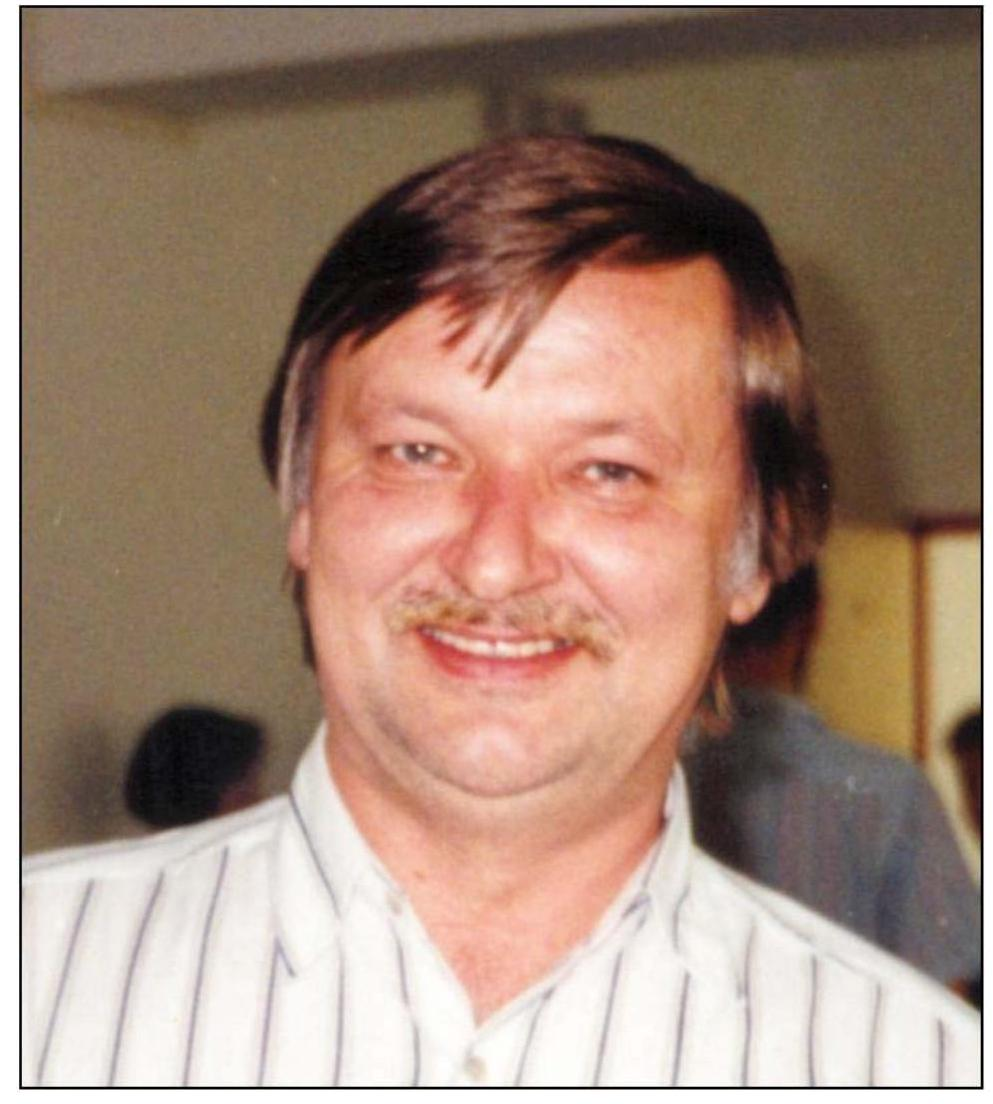
\includegraphics[max width=\textwidth]{2025_02_07_204a351db2d7f48b61ebg-008}
\end{center}

\section*{Tomasz Czosnyka 1952-2006}
This GOSIA manual is dedicated to Tomasz Czosnyka who played a pivotal role in the development of the GOSIA code. Tomasz was a brilliant scientist with tremendous drive, dedication and effectiveness. His work led to pioneering advances in the field of Coulomb excitation. His Ph.D. thesis developed sophisticated techniques that solved a problem that many in the field claimed was impossible when started in 1979. This important development now forms the foundation of modern multiple Coulomb excitation analysis that will continue to play a major role in nuclear physics research at the new radioactive beam facilities now in operation or under construction. Tomasz was a generous, thoughtful friend and colleague with a warm, casual style, and a great sense of humor. Even though Tomasz is no longer with us in person, he is with us in spirit and we continue to hold him in much esteem and affection. The legacy of his achievements in nuclear science will endure for a long time. \{Douglas Cline\}

\section*{Chapter 1}
\section*{Introduction to GOSIA}


\subsection*{1.1 GOSIA suite of Coulomb excitation codes}
Coulomb excitation, which is excitation of nuclear states caused solely by the electromagnetic field acting between the colliding nuclei, is a powerful probe of collective nuclear structure [ALD56, ALD66, ALD75]. The main advantage of Coulomb excitation lies in the fact that, unlike nuclear reactions, the interaction can be described by the well-established theory of the electromagnetic interaction allowing nuclear structure to be studied in a model-independent way. Excitation via the short-ranged nuclear interaction is negligible for bombarding energies well below the Coulomb barrier, whereas the long-ranged electromagnetic interaction still gives rise to a considerable Coulomb excitation. Coulomb excitation is the preeminent probe of collective degrees of freedom in nuclear structure in that it selectively populates collective states with cross sections that are a direct measure of the electromagnetic matrix elements.

The recognition of Coulomb excitation as a method of studying collective motion in nuclei dates back to the early 1950's [ALD56]. Coulomb excitation with light-ion beams was exploited extensively to measure the reduced excitation probabilities and quadrupole moments of the lowest excited states. Experiments performed using light-ion beams can be interpreted relatively easily because first- and second order perturbation theory are applicable since only one and two step excitation processes need to be taken into account (see e.g. the extensive discussion of the perturbation approach in [ALD75] ). The situation changes dramatically for multiple Coulomb excitation that occurs when heavy-ion beams are employed. Multiple Coulomb excitation populates many excited states (up to spin, $40 \hbar$ in strongly deformed nuclei) providing sensitivity to a large body of electromagnetic matrix elements. However, an unfortunate consequence is that perturbation methods are no longer viable. Review papers by Cline [CLI86] and de Boer[BOE84] contain short summaries of the early multiple Coulomb excitation work, complete with extensive lists of references.

A semiclassical theory of multiple Coulomb excitation was developed[ALD56] which led to the first semiclassical multiple Coulomb excitation computer program COULEX developed by Winther and de Boer in 1965[WIN65]. The code COULEX provided the first opportunity to calculate quantitatively multiple Coulomb excitation amplitudes using an assumed set of the reduced electromagnetic matrix elements. This code was a major advance in the field that greatly expanded the exploitation of the powerful Coulomb excitation technique to determine electromagnetic matrix elements in nuclear structure. However, the ultimate goal of a model-independent extraction of the electromagnetic structure parameters (reduced matrix elements) from the heavy-ion experiments was not viable until development, in 1980, of the code GOSIA described in this manual. The main difficulty for making a model-independent analysis lies in the large number of reduced matrix elements influencing heavy-ion excitation. More than a thousand matrix elements can contribute significantly to Coulomb excitation when using heavy beams to excite strongly-deformed nuclei. There are two major tasks to making a model-independent analysis of multiple Coulomb excitation data. The first task is to overdetermine the problem by designing experiments that provide experimental data covering a wide dynamic range of Coulomb excitation strength. The second task is to extract the many unknown matrix elements from this overdetermined data set.

The need to collect Coulomb excitation data for a wide dynamic range of Coulomb excitation interaction strength has led to development of experimental methods to record deexcitation $\gamma$-rays in coincidence with scattered ions over a wide range of particle scattering angle. The efficiency of data collection has been very much enhanced by the development of $4 \pi$ arrays of Compton-suppressed Ge detectors, such as Gammasphere, and large solid-angle, position-sensitive, parallel-plate avalanche detectors that provide mass and scattering angle resolution for detection of both scattered ions in kinematic coincidence. The particle detector allows event-by-event kinematic reconstruction to correct the considerable Doppler shifts of observed $\gamma$-ray energies, dramatically improving the quality of the $\gamma$-ray spectra. Ref. [SIM97] gives technical details of the Rochesterdesigned charged particle detection CHICO, that has been used extensively with Gammasphere for Coulomb excitation studies since 1995.

GOSIA is a powerful suite of semiclassical Coulomb excitation codes developed to both design and analyze multiple Coulomb excitation experiments. These codes were originally developed at the Nuclear Structure Research Laboratory of the University of Rochester in 1980 by Tomasz Czosnyka, Douglas Cline, and ChingYen Wu [CZO83] and development has continued at Rochester, Warsaw, and Köln. The scientific goals are to measure complete sets of $E \lambda$ electromagnetic transition strengths and static moments which provide a sensitive probe of nuclear structure for low-lying nuclear states. GOSIA is specifically designed to handle heavy-ion induced Coulomb excitation where population of many excited states is measured using coincident detection of the scattered ions and the deexcitation $\gamma$-ray decay. This is the only viable technique for such measurements. The GOSIA suite of codes comprises the following computer programes:

\begin{center}
\begin{tabular}{ll}
GOSIA & Designed for simulation and analysis of $p-\gamma$ and $\gamma$ yields due to Coulomb excitation. \\
RACHEL & A GUI for GOSIA to facilitate and simplify the extensive input and output. \\
SIGMA & Quadrupole rotational-invariants fit code \\
GOSIA2 & GOSIA variant designed for measurement of the ratio of target and projectile excitation. \\
PAWEL & GOSIA variant designed to handle an excited isomeric initial state. \\
ANNL & GOSIA variant that uses simulated annealing for the least squares fit. \\
GREMLIN & A code to fit $\gamma$-ray detection efficiency data. \\
\end{tabular}
\end{center}

GOSIA is an experiment-oriented program. Although providing the possibility of running theoretical calculations (i.e. evaluation of excitation amplitudes and $\gamma$-decay yields for a given set of the matrix elements) the primary purpose is to design and analyze experiments that fit matrix elements to best reproduce large experimental data sets. These data not only include the deexcitation $\gamma$-yields observed in a number of independent Coulomb excitation experiments, but also available spectroscopic information, such as branching ratios, $E 2 / M 1$ mixing ratios, nuclear level lifetimes and previously measured $E 1-E 6$, and $M 1$ matrix elements. This combined information allows determination of the full set of matrix elements for an investigated nucleus together with a realistic estimate of the errors of the fitted matrix elements. Finally, using the associated quadrupole rotational invariants code, SIGMA, it is possible, on a basis of the results obtained with GOSIA, to evaluate, in a model-independent way[CLI72, CLI86] the expectation values and the statistical distribution of the $E 2$ moments in the intrinsic frame, providing a clear insight into the collective properties of the nuclear states. Advances in heavy-ion accelerator facilities coupled with significantly more powerful $\gamma$-ray and heavy-ion detector systems has led to a significant increase in the size and complexity of the nuclear systems being studied. Fortunately, this growth in difficulty has been partially matched by a comparable advance in computer technology allowing the code GOSIA to handle the increasingly more complicated systems being analyzed since its inception in 1980.

The code GOSIA is available free for users. However, all users must reference GOSIA[CZO83] in publications based on use of this code. The code has been used extensively since 1980 and appears to contain no significant bugs. Since the code GOSIA is complicated, with extensively overlaid coding, users are strongly advised to seek advice before attempting to make modifications. The goal of the Gosia Steering Committee is to maintain freely available current versions of the GOSIA suite of codes for all users in order to minimize fragmentation of effort and to ensure robust, accurate codes.

\subsection*{1.2 A brief history of Gosia}
The genesis of Gosia dates back to 1965 when multiple Coulomb excitation blossomed due to the advent of heavy-ion accelerators plus the high-resolution Ge $\gamma$-ray detector, coupled with development of the Winther-de Boer semiclassical Coulomb excitation code COULEX [WIN65]. Between 1966 and 1978, Cline and coworkers used heavy-ion beams from the newly commissioned Rochester MP tandem accelerator facility plus the code COULEX to measure static quadrupole moments of the first excited $2^{+}$states via Coulomb excitation [CLI69a, LES70, GER70a, GER70b, LES72, TOW72, CLI73, TOW73, TOW75]. This work initially used a high-resolution magnetic spectrometer. Limitations of this experimental technique led to development of the more powerful particle $\gamma$-ray coincidence technique which necessitated the development at Rochester of the $\gamma$-ray deexcitation code CEGRY[CLI74] that used the statistical tensors calculated by COULEX to predict the subsequent $\gamma$-ray decay properties.

High-Z beams became available with the commissioning of the SuperHILAC at Berkeley in 1975, and the UNILAC at GSI in 1976 which greatly advanced the field of multiple Coulomb excitation. Starting in 1975 Cline, plus coworkers at Rochester, became heavily involved in studies of multiple Coulomb excitation using heavy-ion beams from the SuperHILAC and the Rochester MP tandem. This work involved close collaboration with the Diamond-Stephens group at Berkeley plus Rochester graduate students Ching-Yen Wu and Tomasz Czosnyka. In addition, Julian Srebrny from Warsaw and Lennart Hasselgren from Uppsala each spent a year in Rochester working on this research program. This group, plus other collaborators, were involved in multiple Coulomb excitation studies of ${ }^{104} \mathrm{Ru},{ }^{110} \mathrm{Pd},{ }^{165} \mathrm{Ho},{ }^{166} \mathrm{Er},{ }^{186-192} \mathrm{Os}$, and ${ }^{194} \mathrm{Pt}$.

Population of each state via heavy-ion induced multiple Coulomb excitation results from excitation via many paths involving many $E \lambda$ matrix elements. This strong coupling prevents the use of higherorder perturbation expansion analyses commonly used for light-ion induced Coulomb excitation work. An important question in 1979 was whether it was feasible to unambiguously extract electromagnetic matrix elements from a model-independent analysis of multiple Coulomb excitation data. At that time, many in the field argued that achieving a model independent analysis of multiple Coulomb excitation data was not feasible. The first real breakthrough resulted from use of the codes COULEX plus CEGRY in a modelindependent analysis of the Coulomb excitation data for ${ }^{110} \mathrm{Pd}$ made at Rochester by Lennart Hasselgren [HAS80]. This tour-de-force analysis produced a solution with scientifically interesting implications and provided the proof of principle. Unfortunately there was no practical way to prove the uniqueness of his solution, and the time and effort required to replicate such a manual analysis was impractical. This stimulated the PhD thesis project of Tomasz Czosnyka to develop a Coulomb excitation least-squares search code based on COULEX plus CEGRY in order to provide a practical way of analysing multiple Coulomb excitation data. The development of GOSIA at Rochester proved to be a highly successful project.

The first success of GOSIA was that it proved that the matrix element set found by the manual analysis for ${ }^{110} \mathrm{Pd}$ was the correct solution. Dr Bodan Kotlinski [KOT84] made recoil-distance lifetime measurements in ${ }^{110} \mathrm{Pd}$ which also confirmed the correctness of the solution found using the manual analysis and using GOSIA. In parallel to the ${ }^{110} \mathrm{Pd}$ work, the thesis work of Ching-Yen Wu[WU83, WU89, WU91, WU96] involved an exhaustive analysis of the W-Os-Pt nuclei that was used extensively to develop and test the GOSIA code.

In 1971, based on a suggestion of Kumar[KUM71], Cline and Flaum[CLI72] developed the theory of rotational invariants that directly and model-independently relate observed $E 2$ properties to the intrinsic frame $E 2$ properties. The full potential of this technique was not achieved until development of GOSIA which provided the first viable way to determine a sufficiently complete $E 2$ data set needed to exploit this rotational invariant technique. The success of the Coulomb excitation program achieved two long-sought goals of this group. 1) It proved that multiple Coulomb excitation can be used to model-independently determine signs and magnitudes of fairly complete sets of E2 matrix elements. 2) This set of matrix elements was sufficient for an analysis using the model-independent Rotational Invariant technique[CLI72, CLI86] to extract the expectation values of the centroids and widths in the intrinsic frame for the E2 properties of low-lying states. 3) The E2 rotational invariants provided a powerful probe of collective motion in nuclei in shape-transitional nuclei.

The successful development and exploitation of GOSIA stimulated a rapid growth in multiple Coulomb excitation studies led by the Rochester, Uppsala, Warsaw groups and subsequently the Liverpool group. The GSI based groups were doing similar Coulomb excitation work at the UNILAC in parallel with our collaboration leading to development of a separate analysis code [GRE84], but they eventually switched to\\
the use of GOSIA.\\[0pt]
GOSIA is modelled on the 1978 version[LEL78, BOE84] of the Winther-de Boer code COULEX which extended the code to include multipolarities, $E \lambda$ with $\lambda=1,2,3,4,5,6$ as well as incorporating time-saving updates. The $\gamma$-ray deexcitation part of the code is based on the Coulomb excitation $\gamma$-ray deexcitation code code CEGRY which was developed at Rochester during 1965-75 by Cline, Lesser and Towsley[CLI74]. Significant contributions to the development and testing of GOSIA have been made by additional collaborators. Dr Alexander Kavka [KAV90] tested and elucidated the validity and impact of the deorientation effect, plus he developed the $\gamma$-ray efficiency calibration code GREMLIN.

GOSIA, plus the associated quadrupole rotational-invariants program SIGMA, were developed in 1980. Subsequently three special versions of GOSIA were developed. The first code called GOSIA2 was developed by Czosnyka to handle simultaneous excitation of both target and projectile with common normalization coefficients. The second special code, called PAWEL, is an offspring of GOSIA designed by Czosnyka to handle cases where a fraction of the nuclei have an excited isomeric state as the initial state. The third code ANNL was developed by Richard Ibbotson[IBB95] and exploits simulated annealing techniques to locate least-squares minima.

Tomasz Czosnyka maintained and updated the coding of the GOSIA suite of codes from their inception until his untimely death in October 2006. Under his direction the Warsaw group played a leading role in Coulomb excitation studies is Europe and Japan while Rochester served the same role in the USA.

The GOSIA program was written in Fortran 77 and was originally developed to run on a CDC Cyber 175. The available memory limited the the program size to 130,000 ( 60 -bit) words which complicated the code and required extensive overlaying. From inception in 1980, GOSIA ran with high reliability on many powerful computers. However, by the start of the $21^{\text {st }}$ century the Fortran compilers became less forgiving of archaic Fortran 77 commands and the mixed 32 bit and 64 bit variables in GOSIA resulting in unreliable executables.

Starting in 2007 Dr Nigel Warr, in collaboration with Adam Hayes and Doug Cline, made improvements to the coding of both Gosia and Gosia 2. These programming improvements produced more reliable executables and eliminated bugs. The Warsaw group also started work on upgrades to Gosia including development of a new genetic algorithm procedure to search for multiple minima.

Coordination of future development of Gosia by the user community was recognized as being necessary to forestall splintering of the development effort, to maintain quality assurance, and to handle the growing use of Gosia for Coulomb excitation work at new radioactive plus stable beam facilities. At the Gosia Workshop, held in Warsaw, 8-10 April 2008, it was recommended that a Gosia Users Group be formed to assume responsibility to manage maintanance, standards, and quality assurance testing as well as to promote, prioritize, facilitate, and coordinate development of the Gosia suite of codes. Establishment of a Gosia Users Steering Committee was proposed to implement the goals of the User Group. The participants at the Workshop endorsed establishment of the Gosia Users Group and supported appointment of Douglas Cline (Rochester), Adam Hayes (Rochester), Pawel Napiorkowski (Warsaw) and Nigel Warr (Cologne) to the Gosia Steering Committee.

Starting in April 2008 the Gosia Steering Committee embarked on an ambitious program to upgrade the Gosia suite of codes. The complex intertwined coding of Gosia makes upgrading of the original version of Gosia impractical until partitioning is accomplished thus the long-term upgrade goal involves partitioning the Gosia coding into its separate subroutines to simplify the structure and facilitate future development. Initial coding modifications of GOSIA 2008 have been made made to address the immediate needs of users. These include increasing the dimensions of some arrays and replacing the unreliable Lagrange interpolation procedure with a spline interpolation procedure, incorporating the automatic calculation of internal conversion coefficients, and improving the method for handling of inverse kinematic reactions. Bug fixes include correction of a discontinuity in the TRINT routine and correction of the relativistic correction for projectile excitation. An arsenal of test inputs have been generated to use for quality assurance testing of the upgraded versions of Gosia.

An intuitive graphical user interface shell RACHEL, was developed by Dr Adam Hayes to automate, check, and simplify generation of GOSIA input files as well as to facilitate execution of GOSIA. RACHEL allows fits to user-defined model parameters from several standard collective models of nuclear structure as well as quickly generating simulated data with optional scatter for use in planning experiments.

\subsection*{1.3 GOSIA User support}
\subsection*{1.3.1 Gosia Users Wiki}
The Gosia Wiki (\href{http://www-user.pas.rochester.edu/~gosia/mediawiki/}{http://www-user.pas.rochester.edu/\~{}gosia/mediawiki/}) contains links to download the Gosia programs, the Gosia User Manual, and training videos to support use of RACHEL. The Wiki content is duplicated by the Rochester Gosia website link: \href{http://www.pas.rochester.edu/~}{http://www.pas.rochester.edu/\~{}} cline/Gosia/index.html

\subsection*{1.3.2 Gosia Users Forum}
The Gosia User's Forum ( \href{http://www-user.pas.rochester.edu/~gosia/phpBB3/}{http://www-user.pas.rochester.edu/\~{}gosia/phpBB3/}) provides a conduit to facilitate communication between Gosia users. Adam Hayes manages this site.

\subsection*{1.3.3 Gosia Users Manual}
The Gosia Manual is based on input instructions written by Tomasz Czosnyka, Doug Cline and Ching-Yen Wu. Since 1980 Cline, has expanded, upgraded and maintained the Gosia Manual with major contributions by Adam Hayes, Richard Ibbotson, Alexander Kavka, and Nigel Warr. The present April 2012 version of the User Manual incorporates the major rewrite and expansion performed in 2011.

A comprehensive summary of the Coulomb excitation analysis methods requires knowledge of the algorithms used for this purpose. The effectiveness of data analysis is very much dependent on the ability to select the best ways of using the computer codes, such as GOSIA. Therefore this User Manual is extended beyond the typical program manual to make possible the most efficient utilization of the codes. Chapter 2 was added to aid the user to optimize the design and analysis of Coulomb excitation experiments. A short overview of the semiclassical Coulomb excitation formalism, the theory for subsequent decay of the excited nucleus, the kinematics for inelastic scattering, the Coulomb trajectory, and energy loss, are presented in Chapters 3-5. Chapter 6 describes numerical methods used including the fast Coulomb excitation approximation, which is a basis of GOSIA, GOSIA2, and PAWEL. Chapters 7-13 give detailed input instructions for use of the GOSIA suite of codes plus the RACHEL graphical user interface. Chapter 14 provides a tutorial to introduce the new user on how to compile and use the GOSIA suite of codes. Chapter 15 describes the $\gamma$-ray detector efficiency code GREMLIN thay can be used to calibrate the $\gamma$-ray detection efficiency and correct the measured $\gamma$-ray yields for detection efficiency. Chapter 16 lists the chronology of major changes to the Gosia suite of codes.

\section*{Chapter 2}
\section*{Design and planning of experiments }
The GOSIA suite of codes are ideally suited to the design and planning of heavy-ion induced Coulomb excitation experiments as well as the subsequent analysis. Coulomb excitation experiments can seem deceptively simple, especially for few-state problems, leading some experimenters to fall into analysis traps or collecting data that have less than optimal sensitivity to the goals of the experiment. This chapter identifies a few potential pitfalls in the design and analysis of Coulomb excitation experiments. Additional insight can be obtained from study of prior publications and review articles on heavy-ion induced Coulomb excitation. [ALD75, BOE84, CLI86]

\subsection*{2.1 Theoretical limitations:}
\subsection*{2.1.1 Safe bombarding energy:}
The basic assumption of Coulomb excitation is that the interaction between the scattering ions is purely electromagnetic in origin. This situation applies when the range of nuclear forces for both interacting nuclei are completely separated in space. Coulomb excitation cross sections are maximized by using the highest safe bombarding energy for which the interaction is purely electromagnetic resulting in a sensitive balance between maximizing the cross sections and minimizing the influence of nuclear excitation. The optimal value depends on the goals of the planned experiment. Experimental data on the influence of Coulomb-nuclear interference on the second-order reorientation effect in Coulomb excitation[CLI69a, LES72] was used to estimate the maximum bombarding energy at which the influence of nuclear excitation can be neglected for second-order processes. Near the barrier the Coulomb-nuclear interference is destructive which reduces the inelastic scattering cross sections at large scattering angles in a manner that mimics the reorientation effect corresponding to a negative static quadrupole moment. Figure 2.1 shows the effective static quadrupole moment for the first excited $2^{+}$states of ${ }^{48} \mathrm{Ti},{ }^{56} \mathrm{Fe}$, and ${ }^{60} \mathrm{Ni}$ obtained by Coulomb excitation analyses of inelastic scattering data versus scattering angle for ${ }^{16} \mathrm{O},{ }^{32} \mathrm{~S}$, and ${ }^{35} \mathrm{Cl}$ projectiles. The abscissa corresponds to the classical separation distance for head-on collisions, that is, the distance of closest approach between the nuclear surfaces minus the sum of the nuclear radii. The dashed curves assume an exponential dependence on separation distance fitted to the ${ }^{56} \mathrm{Fe}$ data[LES72, LES74]. Note that the Coulomb-nuclear contribution results in a spurious static quadrupole moment that falls exponentially with separation distance. A safeenergy criterion was selected that corresponds to a minimum separation between the nuclear surfaces of 5 fm required to ensure that the influence of nuclear excitation on the excitation cross sections are $<0.1 \%$. That is, these studies suggest a simple classical safe-energy criterion for reorientation effect studies that the maximum safe bombarding energy for head-on collisions is


\begin{equation*}
E_{\max }(\mathrm{MeV})=1.44 \frac{A_{1}+A_{2}}{A_{2}} \cdot \frac{Z_{1} Z_{2}}{1.25\left(A_{1}^{1 / 3}+A_{2}^{1 / 3}\right)+5} \tag{2.1}
\end{equation*}


\begin{center}
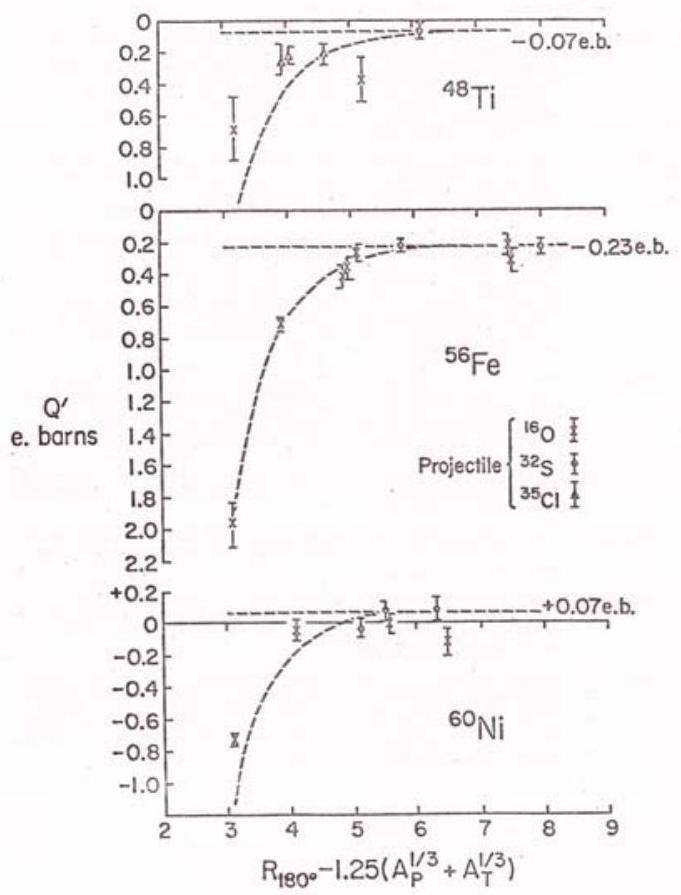
\includegraphics[max width=\textwidth]{2025_02_07_204a351db2d7f48b61ebg-016}
\end{center}

Figure 2.1: Effective values of the static quadrupole moment of the $2_{1}^{+}$states of ${ }^{48} \mathrm{Ti},{ }^{56} \mathrm{Fe}$, and ${ }^{60} \mathrm{Ni}$ extracted from Coulomb excitation reorientation effect data plotted as a function of the classical separation distance between the nuclear surfaces for a head-on collision. [LES72]\\
where index ' 1 ' denotes projectile, ' 2 ' is used for target (this convention will be used repeatedly in this manual). This crude classical safe-energy criterion is applicable only to heavy-ion collisions when the semiclassical approximation is valid, that is, the wavelength is small compared to the distance of closest approach. This naive classical safe-energy criterion is not applicable to light-mass ions, where the semiclassical approximation is not well obeyed, nor is it applicable at above-barrier bombarding energies. Figure 2.2 shows the maximum safe bombarding energy per nucleon corresponding to equation 2.1. The criterion is not meaningful for cases with $Z<6$.

A fully quantal code, such as Ptolemy [MA78, RH80, TOL87], is required to estimate reliably the importance of both Coulomb-nuclear interference effects and quantal effects on Coulomb excitation at near-barrier bombarding energies. Such a calculation was performed by Tolsma[TOL87] for multiple Coulomb excitation of the ground band of ${ }^{238} \mathrm{U}$ by a ${ }^{84} \mathrm{Kr}$ beam at a bombarding energy of 718 MeV . This bombarding energy is twice the safe energy criterion $E_{\max }$ given by equation 2.1. The scattering angle $\theta_{C M}=38^{\circ}$ corresponds to a classical trajectory with $L=520 \hbar$ and distance of closest approach $D_{\text {closest-approach }}=18.2 \mathrm{fm}$ which is the classical safe distance used in equation 2.1. For $\theta_{C M}>38^{\circ}$ the Tolsma calculation predicts increasingly large differences between the excitation probabilities when both the Coulomb and nuclear interaction are included compared with those obtained assuming a pure Coulomb interaction, and these differences are largest for higher-order excitation processes. Figure 2 in the Tolsma [TOL87] paper shows that the phase shift due to the nuclear interaction in the $S$-matrix elements becomes noticable for $L \leq 648 \hbar$ which corresponds to a classical trajectory having a distance of closest approach of 21.58 fm , that is 3.5 fm larger than the 5 fm criterion used in equation 2.1.

Inelastic scattering measurements using above-barrier bombarding energies at scattering angles forward of the grazing angle, corresponding to a distance of closest approach equal to the sum of the nuclear radii, have been exploited to provide reliable qualitative measures of transition strengths for one-step excitation processes[GL98, GL01, CO06]. However, Coulomb-nuclear interference effects on the amplitude and phase of the scattering amplitudes can have a significant impact on cross sections for higher-order excitation processes due to interference of the competing excitation channels. As shown in fig. 2.1, interference can erroneously mimic second-order effects such as the reorientation effect.[CLI69a] Thus higher-order Coulomb\\
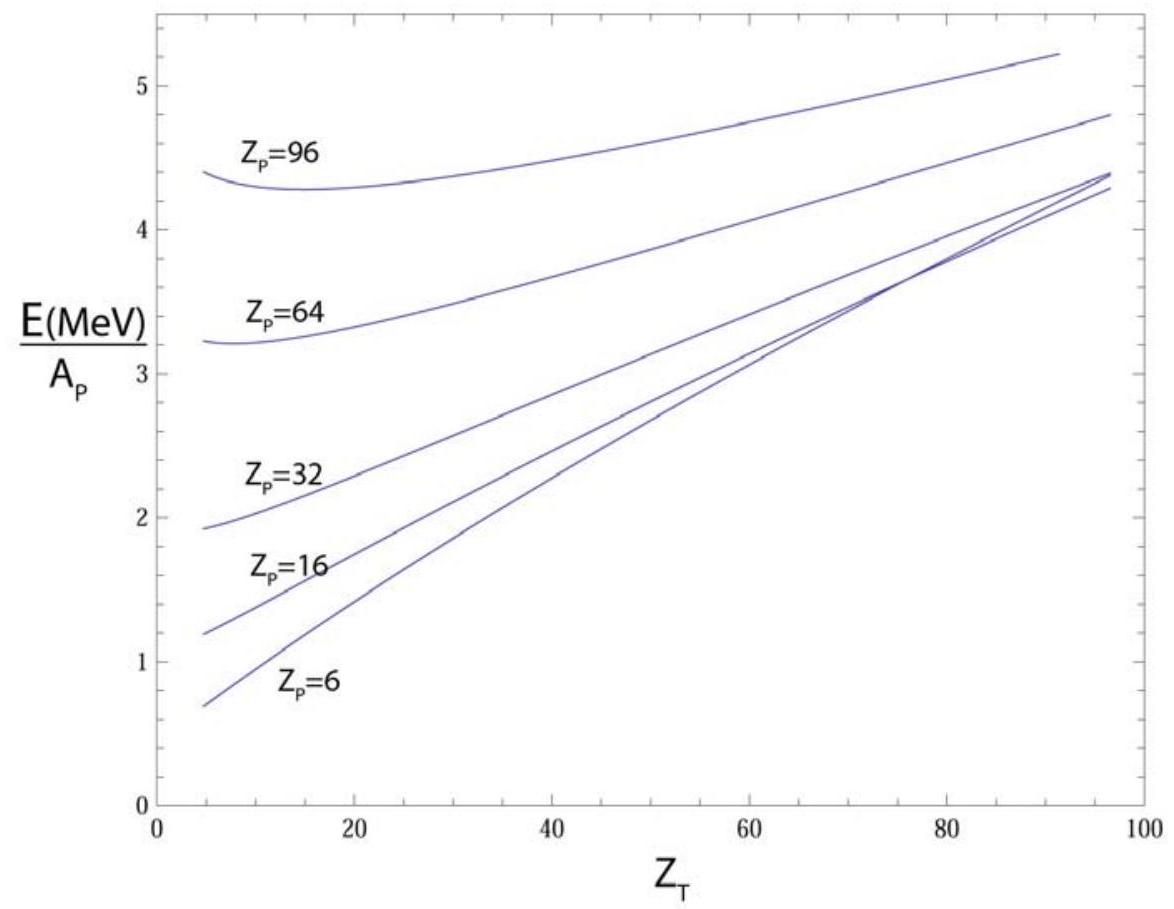
\includegraphics[max width=\textwidth, center]{2025_02_07_204a351db2d7f48b61ebg-017}

Figure 2.2: Maximum safe bombarding energy per nucleon according to equation 2.1 as a function of target $Z_{T}$ value for selected projectile $Z_{P}$. The relation $Z=0.487 \frac{A}{1+0.00602 A^{2 / 3}}$ was used to derive the corresponding A. [ALD75]\\
excitation requires a more stringent safe-energy criterion than single-step excitation in order to extract reliable quantitative measurements of electromagnetic matrix elements.

\subsection*{2.1.2 Semiclassical approximation:}
The long range of the Coulomb interaction, coupled with the small integration step size necessitated by the short wavelength, and the large number of partial waves that make significant contributions, conspire to make it impractical to use full quantal codes on current computers that are capable of handling the large number of coupled channels important to heavy-ion induced Coulomb excitation. Fortunately a considerable simplification can be achieved by assuming a semiclassical treatment of two-body kinematics as pioneered by Alder and Winther[ALD60]. The semiclassical picture exploits the fact that the monopole-monopole Coulomb interaction $Z_{1} Z_{2} e^{2} / r$ dominates and determines the relative motion of the two colliding nuclei. The semiclassical picture assumes that the size of the incoming projectile wavepacket is small compared to the dimensions of the classical hyperbolic trajectory which is expressed in terms of the Sommerfeld parameter:


\begin{equation*}
\eta=\frac{2 \pi a}{\lambda}=\frac{Z_{1} Z_{2} e^{2}}{\hbar v_{I}} \gg 1 \tag{2.2}
\end{equation*}


Here $a$ denotes half the classical distance of closest approach for a head-on collision, $\lambda$ is the wavelength of the incoming projectile with initial velocity $v_{I}$, while $Z_{1} e$ and $Z_{2} e$ are the charges of the projectile and target respectively. The second requirement of the semiclassical picture is that the energy loss is much smaller than the incident energy, i.e.


\begin{equation*}
\frac{\Delta E}{E} \ll 1 \tag{2.3}
\end{equation*}


For typical heavy-ion induced Coulomb excitation, equations 2.1 and 2.2 yield values of $\eta$ ranging from 10 to 500 for $Z_{p r o j} \geq 6$ and $Z_{T}>10$ as illustrated in figure 2.3 . Note that the validity of a classical description of the scattering kinematics is closely connected to the assumption of non-intervention of the nuclear forces.\\
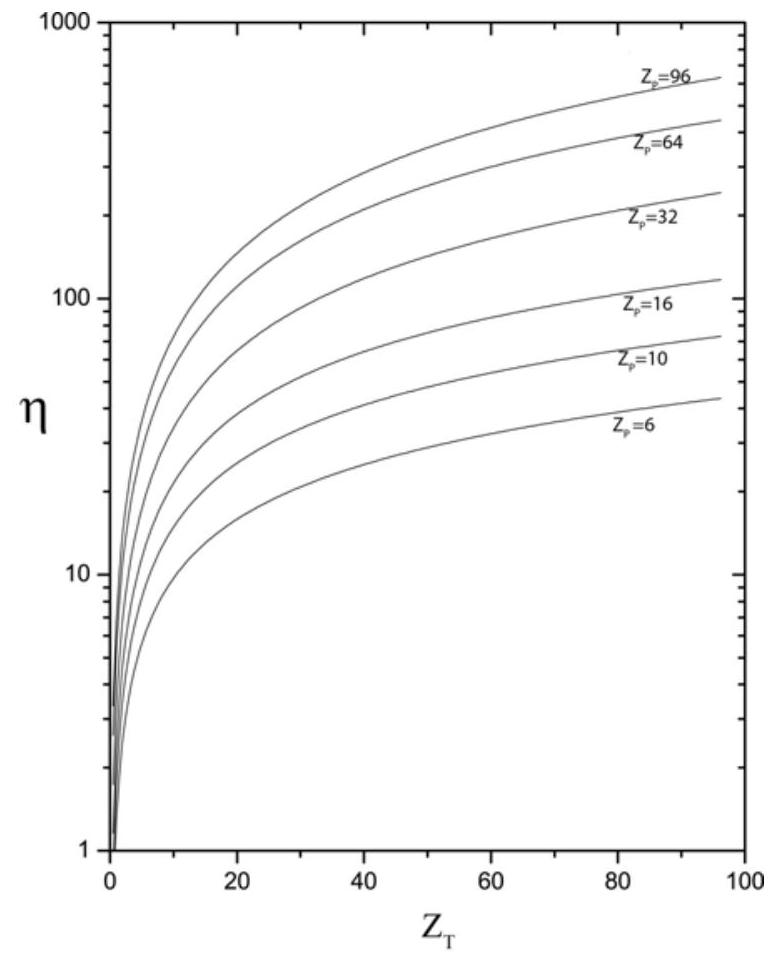
\includegraphics[max width=\textwidth, center]{2025_02_07_204a351db2d7f48b61ebg-018}

Figure 2.3: The Sommerfeld parameter $\eta$ at the safe bombarding energy as a function of target $Z_{T}$ for various projectile $Z_{P}$.

The semiclassical approach is applicable par excellence for all heavy-ion processes when the interaction is purely electromagnetic. The semiclassical approximation is not useful for Coulomb excitation of light nuclei with $Z<6$ because of the decrease in accuracy for the higher excitation energies of typical states in light nuclei. Fortunately the few states excited in light nuclei make it feasible to perform fully-quantal Coulomb excitation calculations for such cases.

The accuracy of the semiclassical approximation improves with increase of the Sommerfeld parameter $\eta$. The use of energy-symmetrized orbits in the semiclassical calculations partially corrects for the $Q$ value dependence which is the largest deficiency in the semiclassical approximation. The remaining quantal corrections to the calculated cross sections are of the order of $1 / \eta$ for large $\eta$. Full quantal calculations by Kavka[KAV90] show that semiclassical calculations differ from full quantal predictions by typically $3 \%$, with some values as much as $10 \%$ off. These agree with the predictions of Tolsma [TOL79] for the case of ${ }^{238} \mathrm{U}$ excited by $385 \mathrm{MeV}{ }^{84} \mathrm{Kr}$ ions. Note that heavy-ion induced Coulomb excitation data typically involves a comparison of the relative deexcitation $\gamma$-ray yields which tends to cancel part of this systematic error[KAV90, STA82].

The semiclassical approach elucidates the time evolution of the excitation of the excited states as the projectile moves along the classical hyperbolic trajectory. Figure 2.4 shows an example of the time evolution of excitation probabilities for the ground rotational band of ${ }^{238} \mathrm{U}$ excited by backscattered $140 \mathrm{MeV}{ }^{40} \mathrm{Ar}$ ions. The zero of time corresponds to the classical turning point and most of the excitation occurs within $\pm 15 \mathrm{fm}$ of the turning point. The final population distribution is shown on the right hand side. Note that the time scale of the excitation is the order of $3 \times 10^{-21} s$ which is $10^{8}$ times shorter than typical lifetimes for $\gamma$-ray decay which are $10^{-13}-10^{-12} s$. Thus the assumption that the excitation and decay processes are separate and sequential processes is valid.

\subsection*{2.1.3 Adiabaticity constraints:}
Advances in detector technology have resulted in a tremendous increase in experimental detection sensitivity that has led to the need to calculate Coulomb excitation cross sections for high-energy transitions that can\\
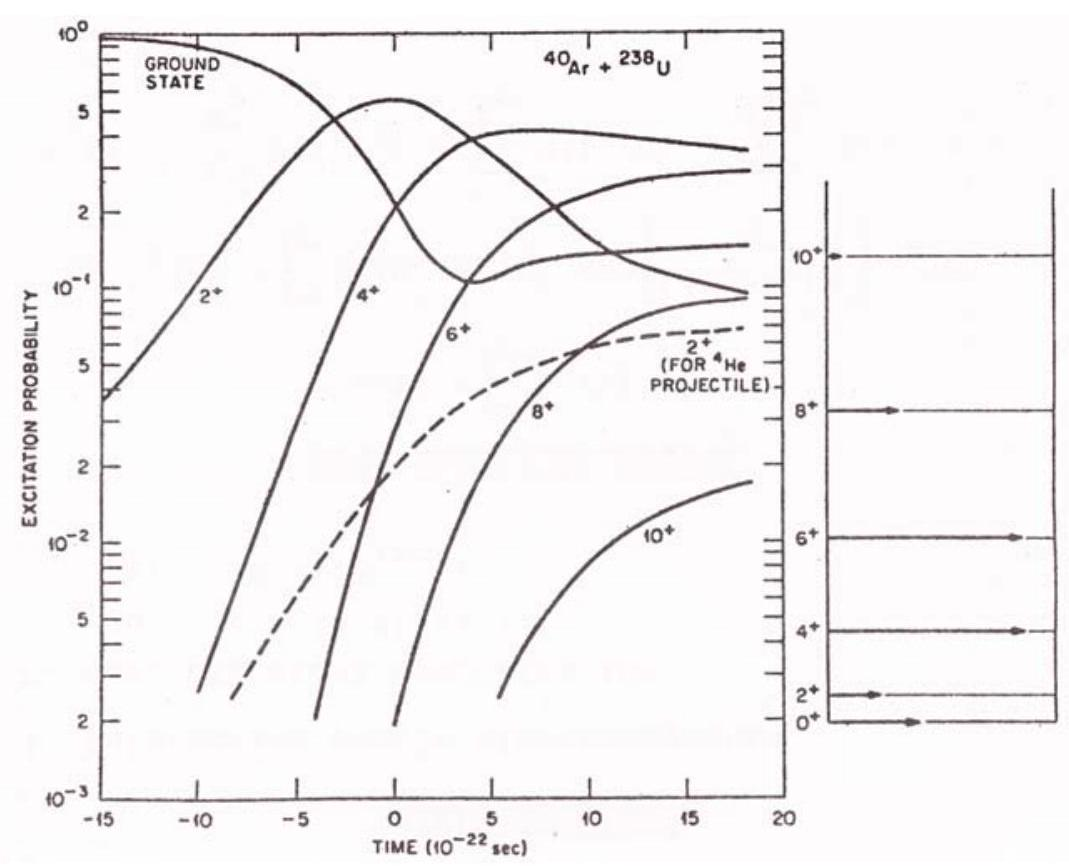
\includegraphics[max width=\textwidth, center]{2025_02_07_204a351db2d7f48b61ebg-019}

Figure 2.4: Semiclassical Coulomb excitation predictions of the time evolution for excitation of the groundband in ${ }^{238} \mathrm{U}$ by backscattered $140 \mathrm{MeV}{ }^{40} \mathrm{Ar}$ ions. [MCG69]\\[0pt]
challenge the adiabaticity limitations built into the 1980 version of GOSIA [CLI08]. As discussed in section 6.3, numerical integration of the semiclassical Coulomb excitation amplitudes for Coulomb excitation can be problematic in the asymptotic regions of the classical hyperbolic trajectory because of the exponential increase in the oscillatory frequency of the integrand when the product of the adiabaticity and orbit eccentricity is large. In the far asymptotic region the period of the oscillatory exponent of the integrand becomes comparable to the step size used during numerical integration which can lead to pathological behaviour. This is primarily a problem at the the longest ranges that are required to evaluate $E 1$ excitation of high-lying states. For $E 1$ or $E 2$ Coulomb excitation of high-lying states it behoves the user to ensure that the numerical integrations are free of pathological behaviour due to high adiabaticity transitions with high eccentricity trajectories. Note that the GUI Rachel provides optional tests for violation of the adiabaticity limits.

\subsection*{2.1.4 Hyperfine interaction:}
In typical Coulomb excitation experiments, both the scattered projectile and target nuclei recoil into vacuum in highly-excited, highly-ionized, atomic states which subsequently decay to a ground state. The strong fluctuating hyperfine fields of the deexciting atom depolarize the nuclear state alignment; this effect is known as the nuclear deorientation effect. This attenuates the angular distribution of the de-excitation $\gamma$-rays which can be taken into account by introducing the spin and lifetime dependent attenuation coefficients $G_{k}$ that multiply the decay statistical tensors. The lack of a viable way to accurately predict the time-dependent hyperfine atomic fields is the major theoretical uncertainty in Coulomb excitation experimental studies. Unfortunately the atomic hyperfine fields involve complicated stochastic processes that currently cannot be predicted. When the nucleus recoils out of the target the highly-ionized and highly-excited atomic structure decays rapidly by a cascade of photons, as well as Auger electrons, with time constants as short as a picosecond. This rapid atomic decay produces a rapidly fluctuating hyperfine atomic field. Eventually the atomic structure deexcites to the equilibrium atomic ground-state configuration which depends on the charge state of the ion. The deorientation effect has a complicated dependence on the recoil velocity, the lifetimes of the excited states, the atomic and nuclear spins, and dephasing effects. Since these complicated and stochastic atomic processes cannot be predicted accurately at the present time it is necessary to resort to simple models with parameters fitted to available deorientation effect data. Fortunately the Two-state\\[0pt]
model[BOS77, BRE77], currently built into GOSIA, correlates well with experimental data on the deorientation effect[KAV90]. Also the use of $4 \pi \gamma$-ray detector arrays washes out sensitivity to the angular correlation effects for $\gamma$-ray deexcitation.

\subsection*{2.2 Technical requirements}
\subsection*{2.2.1 Optimal data requirements:}
Coulomb excitation is the preeminent technique for making precise measurements of electromagnetic matrix elements which provide a sensitive probe of nuclear structure. Extraction of the many $E \lambda$ matrix elements involved in heavy-ion induced Coulomb excitation requires collection of data over a wide dynamic range of Coulomb interaction strength in order to significantly overdetermine the system of many strongly-coupled excitation channels and avoid spurious correlations. The following experimental methods can be used to collect data over a sufficiently wide range of Coulomb interaction strength to enhance sensitivity.

\begin{enumerate}
  \item Record data over a wide range of scattering angles, that is, impact parameters, for a given beam species to excite the nucleus of interest.
  \item Record data over a wide range of bombarding energies.
  \item Record data using a wide range of $Z$ values for the nucleus used to excite the nucleus of interest.
  \item Combine Coulomb excitation yields with precise measurements performed using other techniques such as recoil-distance lifetime measurements.
  \item Record $\gamma-\gamma$-ray coincidence data to determine $\gamma$-ray decay schemes, branching ratios, mixing ratios etc.
\end{enumerate}

Measurements using methods 1 , and 5 can be performed simultaneously using $4 \pi$ arrays of particle and $\gamma$ ray detectors which minimizes use of beam time. Methods 2,3 , and 4 require several experiments involving use of more beam time which is of consequence when using expensive and oversubscribed accelerator facilities. The beam-time requirements are more stringent when recording data sufficient to exploit the rotationalinvariant method. For example, methods $1,3,4$, and 5 were used for measuring rotational invariants. Precise measurements of excited state lifetimes via other techniques reduces the number of coupled channels sensitive to the data which simplifies the Coulomb excitation analysis.

\subsection*{2.2.2 Experimental detection techniques:}
The following are the main experimental detection techniques used for Coulomb excitation studies.

\section*{High-resolution particle spectroscopy:}
High-resolution particle spectroscopy is a precise and direct method for measuring Coulomb excitation cross sections[CLI69a]. The simultaneous measurement of the elastic and inelastic channels eliminates many sources of systematic errors. The disadvantages of this method are that adequate energy resolution is achieved only when using light ions in conjunction with very thin targets. The experimental sensitivity is very poor due to a background resulting from elastic scattering by target contaminants. This method is of most value for one-step Coulomb excitation measurements using high-intensity beams of stable light nuclei; it is not viable for use with weak rare-ion beams.

\section*{High-resolution $\gamma$-ray spectroscopy:}
Gamma-ray spectroscopy using high-resolution Ge $\gamma$-ray detector arrays is the only viable experimental technique for resolving the many states Coulomb excited when heavy ions and thicker targets are utilized. Unfortunately, the recoil velocities of the excited target nuclei typically are large, $v / c \leq 0.1$, which leads to considerable Doppler shift and Doppler broadening of detected $\gamma$-rays for in-flight decay of ions recoiling in vacuum. Consequently, detection of deexcitation $\gamma$-rays, without simultaneous measurement of the recoil\\
direction and velocity of the recoiling emitter, is of limited value for Coulomb excitation work due to the low energy resolution. Use of a target thick enough to stop the recoiling excited nuclei produces Doppler broadened $\gamma$-ray line shapes for states that decay during the slowing-down time of the recoiling ion in the target, and sharp lines for transitions decaying after the recoiling ions have stopped. Observation of $\gamma-\gamma$ or higher-fold $\gamma$-ray coincidences, using high-resolution $\gamma$-ray detector arrays, without gating on recoil angle and energy, is sensitive and ideally suited to elucidation of level and $\gamma$ decay schemes for states having lifetimes $\tau>10^{-13} s$, but the intensities of shorter-lived states are poorly measured. Moreover, only one intensity per $\gamma$-ray transition is measured which is insufficient to overdetermine the system of coupled channels. In addition, extensive computation is required for integrating the Coulomb excitation cross sections over scattering angle and recoil energy. As a consequence, recording of coincident $\gamma-\gamma$ data, without recoil-ion detection, is of limited use for measurement of electromagnetic matrix elements by Coulomb excitation. This type of data has to be normalized to a known transition strength in either the target or projectile in order to extract electromagnetic matrix elements and error estimation is difficult.

\section*{High-resolution coincident $p-\gamma$-ray spectroscopy:}
Currently high-resolution coincident $p-\gamma$-ray spectroscopy, using $4 \pi$ arrays of recoil-ion and $\gamma$-ray detectors, is the most viable experimental technique for study of heavy-ion induced Coulomb excitation which stimulated development of the code GOSIA in 1980. Detection of the deexcitation $\gamma$-ray, in coincidence with the recoiling deexciting nucleus, can specify the recoil direction and recoil velocity allowing the individual $\gamma$-ray signals to be corrected for the Doppler shift on an event-by-event basis. Detection of the recoiling ion velocity and direction can be performed with sufficient accuracy using targets up to several $\mathrm{mg} / \mathrm{cm}^{2}$ in thickness. Use of $4 \pi$ heavy-ion and $\gamma$-ray detector arrays for Coulomb excitation measurements provides simultaneous measurement over a wide range of scattering angles, identification of the scattered ion species, optimal energy resolution of the deexcitation $\gamma$-rays, and allows use of $p-\gamma-\gamma$, plus higher fold coincidences, to greatly improve the experimental sensitivity. The absolute cross sections can be derived either by normalizing to the scattered particle singles or to transitions for which the transition strength has been measured previously. For Coulomb excitation of strongly-deformed nuclei, the $\gamma$-ray deexcitation yields of low-lying ground-band transitions provide a precise normalization for determination of absolute $B(E \lambda)$ transition strengths as discussed in section 2.3.1.

The Rochester collaboration has employed $4 \pi$ arrays of position-sensitive parallel-plate avalanche gas detectors for Coulomb excitation studies with considerable success for more than three decades. The current heavy-ion detector $\mathrm{CHICO}[\mathrm{SIM} 97]$ covers $67 \%$ of $4 \pi$, detects scattered ions in kinematic coincidence over a scattering angle range of $12^{\circ} \leq \theta \leq 168^{\circ}$ with angle resolution of $\Delta \theta=1^{\circ}$ and $\Delta \phi=4.6^{\circ}$, and with a time resolution $\Delta \tau=0.7 n s$.[SIM97] CHICO provides a mass resolution of $\Delta m / m=5 \%$ and $Q$-value resolution of $\Delta Q \leq 20 \mathrm{MeV}$ assuming two-body kinematics. CHICO is rugged to radiation damage, can handle high count rates, and has low mass that minimizes degradation of the $\gamma$-ray detector performance. The current upgrade of CHICO to CHICO-2 will improve the $\phi$-angle resolution to $\Delta \phi=1^{\circ}$ needed to fully exploit the performance of the $\gamma$-ray tracking array, GRETINA. The Warsaw group has used large solid-angle arrays of PIN diodes for heavy-ion detection[WUE03]. Large annular double-sided position-sensitive silicon detectors have been used extensively for Coulomb excitation of rare-ion beams since their susceptibility to radiation damage is less of a problem when using weak beam intensities.

The $4 \pi$ solid-angle, high-resolution Ge detector arrays, such as Gammasphere[GS98], TIGRESS, and MiniBall, currently are the premier $\gamma$-ray detectors for use in Coulomb excitation measurements since their high detection efficiency allows use of $p-\gamma-\gamma$ and higher-fold coincidence resulting in a tremendous increase in resolving power and sensitivity. Coincident $\gamma$-ray spectra in typical heavy-ion Coulomb excitation studies using CHICO plus Gammasphere achieve an overall average Doppler-corrected $\gamma$-ray energy resolution of $0.9 \%$ FWHM. This resolution is limited by the finite size of the individual Ge detectors. The improved angle resolution of the $\gamma$-ray tracking array GRETINA plus the improved $\phi$ resolution of CHICO2 should reduce this energy resolution to about $0.3 \%$ providing a 9 -fold improvement in sensitivity and resolving power for $p-\gamma-\gamma$ events.

Figure 2.5 shows Coulomb excitation $\gamma$-ray spectra for a $1358 \mathrm{MeV}^{238} \mathrm{U}$ beam bombarding a $500 \mu \mathrm{~g} / \mathrm{cm}^{2}{ }^{170} \mathrm{Er}$ target. Note that the raw Doppler-broadened spectrum shows only one sharp line at 934 keV due to a 42.8 ns isomeric decay of a $1268.6 \mathrm{keV} 4^{-}$state in ${ }^{170} \mathrm{Er}$ that stops in the detectors prior to decay. Doppler correction clearly resolves transitions for either target or projectile excitation. That is, the correct Doppler shift gives\\
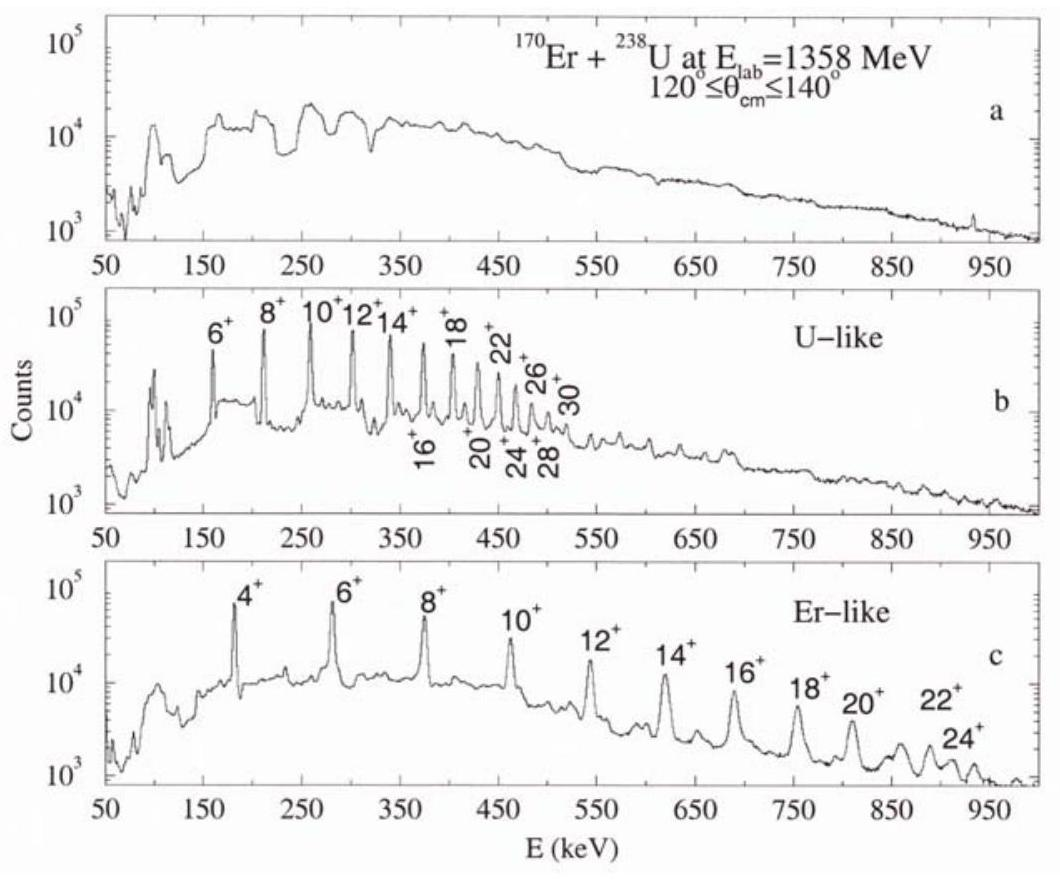
\includegraphics[max width=\textwidth, center]{2025_02_07_204a351db2d7f48b61ebg-022}

Figure 2.5: Typical $\gamma$-ray spectra for $1358 \mathrm{MeV}{ }^{238} \mathrm{U}$ beam on a $0.5 \mathrm{mg} / \mathrm{cm}^{2}{ }^{170} \mathrm{Er}$ target detected using Gammasphere in coincidence recoil ions detected by CHICO. (a) shows the raw coincident $\gamma$ ray spectrum, (b) shows the coincident $\gamma$ ray spectrum Doppler-corrected for $U$ recoils, (c) shows the coincident $\gamma$ ray spectrum Doppler-corrected for Er recoils. [WU00]\\
sharp lines on a broad background of incorrectly shifted $\gamma$-transitions from the partner nucleus. The high recoil velocities of the ${ }^{170} \mathrm{Er}$ recoils is the reason for the poorer energy resolution in spectrum $2.5 c$.

Figure 2.6 illustrates the cleanliness and sensitivity of $p-\gamma$ Doppler-corrected spectra for a typical spectrum for Coulomb excitation of a $985 \mathrm{MeV}{ }^{178} \mathrm{Hf}$ beam by a $0.5 \mathrm{mg} / \mathrm{cm}^{2}{ }^{208} \mathrm{~Pb}$ target and recorded using CHICO plus Gammasphere. Note that the peak to background ratio for ground-band transitions is $\approx 70 / 1$ even for detection of only one $\gamma$-ray. The $p-\gamma-\gamma$ spectra are much cleaner and provide a much higher sensitivity [HAY10b]. Gating on delayed deexcitation $\gamma$-rays from isomeric states with lifetimes in the $n s$ to $\mu s$ range provides higher sensitivity $p-\gamma-\gamma$ spectra both for prompt transitions feeding the isomer, and for decay of the isomer.

A useful variant of the $p-\gamma-\gamma$ technique uses a thick target to stop the excited recoils in the target. The deexcitation $\gamma$-rays are detected in coincidence with backscattered heavy-ions which provides $\gamma$-ray spectra with the intrinsic energy resolution of a Ge detector and the cleanliness of the $p-\gamma$ technique. An example is a study of the Coulomb excitation of a ${ }^{235} \mathrm{U}$ target by a $184 \mathrm{MeV}{ }^{40} \mathrm{Ca}$ beam which resulted in observation of $\approx 300$ resolvable $\gamma$-ray transitions between $150-1700 \mathrm{keV}$ which greatly expanded the known spectroscopy for this nucleus[WAR05, WAR12]. Another example is Coulomb excitation of the odd-odd isomeric nucleus ${ }^{242} \mathrm{Am}$ by a $170.5 \mathrm{MeV}{ }^{40} \mathrm{Ar}$ beam[HAY10]. Unfortunately the Doppler-broadened line shapes limit the usefulness of such thick-target data for extraction of electromagnetic matrix elements.

The calculation of $p-\gamma-\gamma$ angular correlations has not been implemented in GOSIA. However, high sensitivity $p-\gamma-\gamma$ data, collected using a $4 \pi$ detector, such as Gammasphere, can be analysed by using $4 \pi$ detection of the gating $\gamma$-ray transitions to eliminate the need to know the $p-\gamma-\gamma$ angular correlation and by correcting the yields of interest using the measured $\gamma$-ray branching ratios. Summing over many gates can improve the statistics for the gated $\gamma$-ray spectra.

\subsection*{2.2.3 Projectile Coulomb excitation}
The experimental sensitivity for Coulomb excitation of target nuclei usually is limited by the isotopic purity of the target. That is, the weakly-populated states of interest are swamped by Coulomb excitation of strongly-\\
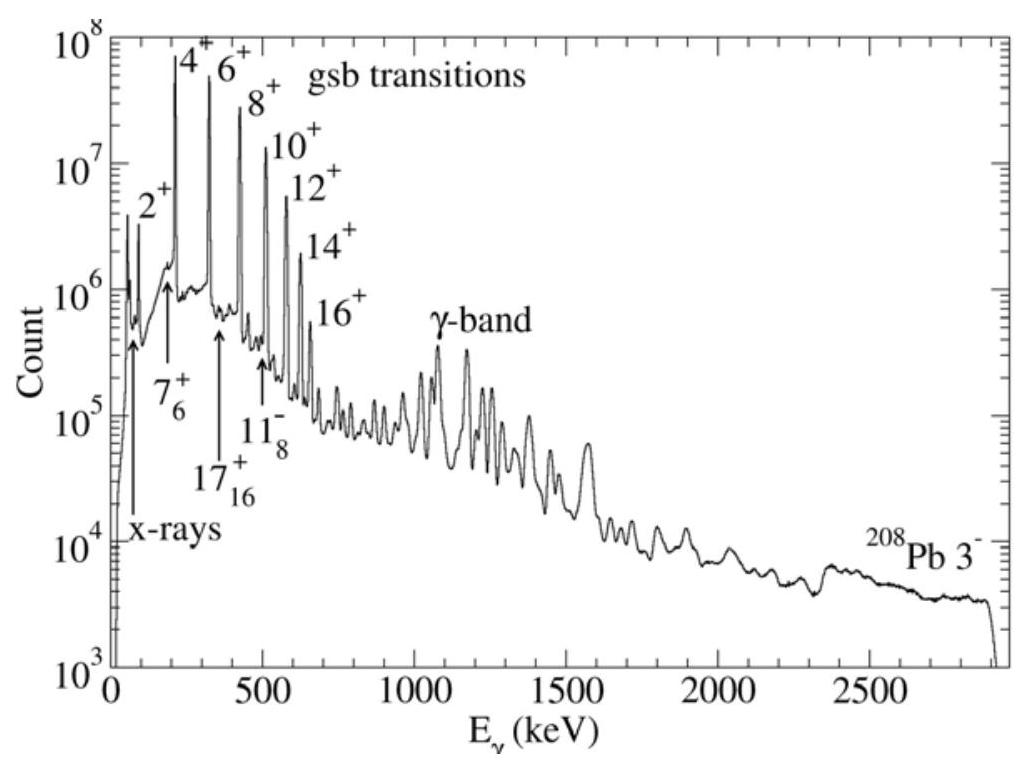
\includegraphics[max width=\textwidth, center]{2025_02_07_204a351db2d7f48b61ebg-023}

Figure 2.6: A recoil- $\gamma$-ray coincidence spectrum for projectile scattering angle range $35^{\circ} \leq \theta \leq 50^{\circ}$ obtained using a $985 \mathrm{MeV}{ }^{178} \mathrm{Hf}$ beam bombarding a $0.5 \mathrm{mg} / \mathrm{cm}^{2}{ }^{208} \mathrm{~Pb}$ target. The $\gamma$-ray spectrum is Doppler corrected for ${ }^{178} \mathrm{Hf}$. In-band transitions in the ground band, and $\gamma$-band to ground band transitions are cleanly resolved. The $3^{-} \rightarrow 0_{g s b}$ in ${ }^{208} \mathrm{~Pb}$ has been broadened due to use of the wrong Doppler correction. [HAY10b]\\
populated transitions in adjacent isotopic contaminants in the target that have similar transition energies to those of interest. The isotopic purity of accelerated beams usually is considerably higher than that available using isotopically-enriched targets. As a consequence projectile Coulomb excitation can provide significantly higher sensitivity than target excitation for Coulomb excitation studies. Targets used for projectile Coulomb excitation work can be selected to have high isotopic purity, to be closed-shell nuclei minimizing target excitation, and the Doppler shift can be used to discriminate target deexcitation from projectile deexcitation. Another advantage of projectile Coulomb excitation is that the hyperbolic trajectories leading to the strongest Coulomb excitation usually result in $\gamma$-ray deexcitation at lower recoil velocities than for target excitation which reduces the resultant Doppler broadening. Projectile Coulomb excitation is the only viable approach for studies of rare-ion beams.

\subsection*{2.2.4 Inverse kinematics}
The use of inverse kinematics, that is, $\frac{m_{T}}{m_{P}}<1$, has technical advantages in that recoil ion detectors are required only in the forward hemisphere which simplifies recoil-ion detection, and the recoil-ion velocities are higher which enhances recoil-ion detection. As shown in figure 5.2, inverse kinematics leads to two-valued center-of-mass scattering angles for each projectile or target recoil angle.

As discussed in section 5.2, for inverse kinematics the scattered projectile has a maximum scattering angle given by

$$
\sin \theta_{\max }=\frac{m_{T}}{m_{P}} \sqrt{1-\frac{\Delta E}{E_{P}}\left(1+\frac{m_{P}}{m_{T}}\right)}
$$

where $m_{P}, m_{T}$ are the projectile and target masses, $E_{P}$ is the bombarding energy, and $\Delta E$ is the excitation energy. Note that for elastic scattering the maximum angle is independent of the bombarding energy which is not true for inelastic scattering. Only recoil target nuclei are detected for target recoil angles $\theta_{T}>\theta_{\max }$ which eliminates the need to discriminate between recoiling target and projectile nuclei. This trick has been employed frequently for studies of projectile Coulomb excitation by thin ${ }^{12} \mathrm{C}$ targets which minimizes multiple Coulomb excitation. Such small $\frac{m_{T}}{m_{P}}$ ratios have the advantage that the maximum angle of the scattered projectiles is small, e.g. $\theta_{\max }=8.6^{\circ}$ for $m_{P}=80$, allowing unambiguous detection of the ${ }^{12} \mathrm{C}$ target recoils at larger angles. Note that for a given target recoil angle there is a second kinematic solution\\
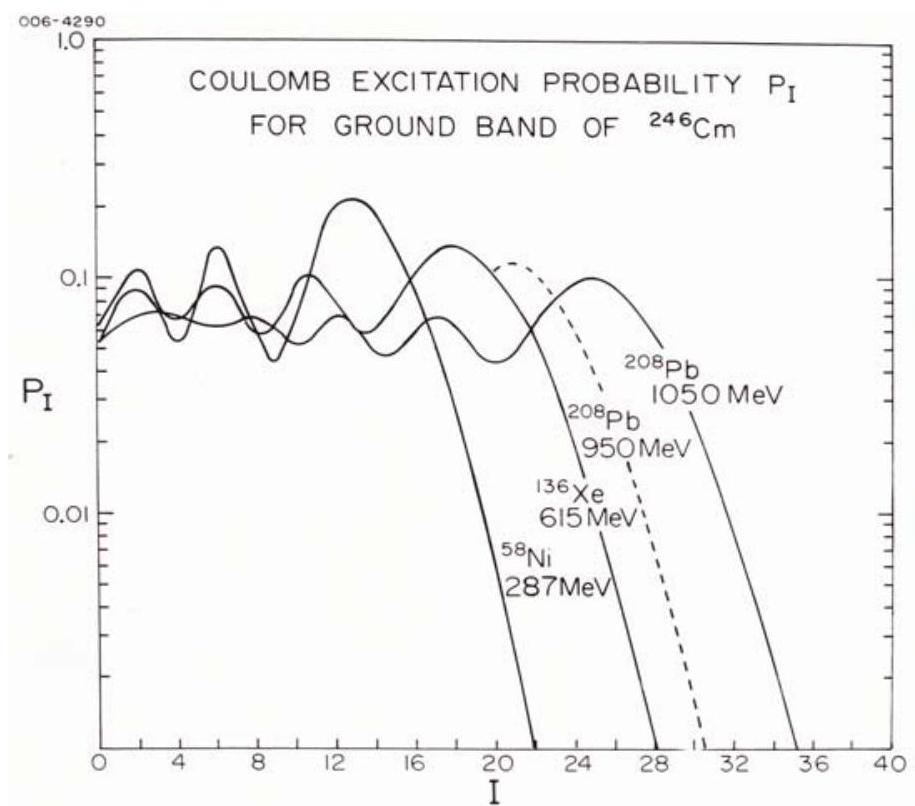
\includegraphics[max width=\textwidth, center]{2025_02_07_204a351db2d7f48b61ebg-024}

Figure 2.7: The calculated probability for Coulomb excitation of the ground band of ${ }^{246} \mathrm{Cm}$ by backscattered ions. The E2 matrix elements were assumed to be related by the spheroidal rotor relation. [CLI86]\\
for inelastic scattering that corresponds to centre-of-mass scattering angle close to zero. This second solution is of no practical consequence since target-recoil energies for this second solution typically are the order of 100 keV leading to these recoils being either stopped in the target or being below the recoil detect threshold. Gosia/Rachel are designed to automatically calculate recoil-target detection for inverse kinematics. Care must be taken to ensure that recoil-ion detection thresholds do not further restrict the angular range of detected particles.

Note that it is not sensible to only detect recoils at angles $\theta<\theta_{\max }$ since then both projectile and target recoils will be observed with comparable detection energies, and for each projectile detection angle there are two centre-of-mass scattering angles which lead to different Coulomb excitation cross sections. Gosia/Rachel are not designed to automatically handle the double-valued solution for recoiling projectiles. Experiments using such a geometry would require separate calculations of each of the solutions and manually summing them.

Note that detection of both projectile and target recoils in kinematic coincidence completely and unambiguously identifies the sections of the kinematic curve involved in Coulomb excitation measurements.

\subsection*{2.3 Sensitivity to observables}
\subsection*{2.3.1 Transition strengths}
A primary goal of Coulomb excitation work is the measurement of $B(E \lambda)$ transition strengths. In the perturbation limit the excitation probability of an excited state $J_{2}$ is directly proportional to the $B\left(E \lambda ; J_{1} \rightarrow\right.$ $J_{2}$ ). However, multistep processes, which dominate for heavy-ion induced multiple Coulomb excitation of strongly-deformed nuclei, can lead to a wide range in sensitivities of multiple Coulomb excitation data to individual electromagnetic matrix elements. Figure 2.7 shows the calculated excitation probability for target excitation of the ground band of ${ }^{246} \mathrm{Cm}$ for backscattered heavy-ions. The population probability is roughly uniform up to a spin value that depends on the strength of the Coulomb interaction, followed by a rapid drop in excitation probability at higher spin. For example, for $1050 \mathrm{MeV}{ }^{208} \mathrm{~Pb}$, the excitation probability oscillates about an average value of $\approx 8 \%$ up to spin 24 , and the ground-state population is more weakly populated than some higher ground-spin states. Note that the deexcitation $\gamma$-rays feed down the ground band resulting in $\approx 90 \%$ of the $\gamma$-ray strength feeding through the lowest $2_{g s b}^{+} \rightarrow 0_{g s b}^{+}$. As a consequence\\
the yield of the lowest $\gamma$-ray transitions in the ground-band of a strongly deformed nucleus are relatively insensitive to the $B(E \lambda)$. Although this insensitivity may appear to be a disadvantage, it actually is useful since the coincident deexcitation $p-\gamma$-ray yields for the low-lying ground-band states provide a precise normalization for accurate measurement of absolute $B(E \lambda)$ values of higher-lying and weakly populated states.

The calculated excitation probability sensitivity parameters $\alpha_{k i}^{P}$ for state population is defined by the relation

$$
\alpha_{k i}^{p} \equiv \frac{\Delta M_{i}}{M_{i}} \frac{P_{k}}{\Delta P_{k}}
$$

where $M_{i}$ is a matrix element and $P_{k}$ the excitation probability for state $k$. In the perturbation limit $\alpha_{k i}^{p} \approx 2$ but can be much smaller due to multistep processes and $\gamma$-ray feeding. The difference in sensitivity with scattering angle, $Z$, and bombarding energy is exploited to determine individual matrix elements from the system of strongly-coupled channels. Higher-fold $p-\gamma-\gamma$ coincidence data are desirable for measurement of $B(E \lambda)$ values connecting to the side bands which are a sensitive probe of nuclear structure.

Coulomb excitation cross sections are sensitive to both the magnitude and relative signs of the coupled channels contributing to population of excited states, and these signs are related to the relative signs of the individual matrix elements. Although the phase of a wavefunction is arbitrary, it is best to fix the phases of states to conform to a logical convention, rather than allowing a random selection, to facilitate comparison with nuclear structure models. Choosing one matrix element between two states to be positive couples the relative phases of the wavefunctions of these two states to be the same. Then the phases of any other matrix elements coupling these two states, relative to the phase of the positive one, are observables. Consequently for typical collective bands it is convenient to choose the primary $\Delta I=2, E 2$ transitions in the band to have a positive phase, which locks the signs of the wavefunctions of the states in a band to have the same phase. In addition the phase of one strong matrix element connecting two separate collective bands locks the relative phase between the states in these two collective bands. For convenience the phases usually are locked to correspond to the phase convention used by rotational collective models.

Coulomb excitation is most sensitive to the $E 1, E 2$, and $E 3$ multipole excitation but in nuclei the $E 1$ excitation is negligible because the $E 1$ strength is exhausted by the high-lying giant dipole resonance. This giant dipole resonance is not populated due to the high excitation energy. Thus $E 2$ and $E 3$ are the multipoles studied since typically the $E 4$ excitation mode can be neglected. Magnetic excitation is negligible for subbarrier Coulomb excitation. However, $B(M 1)$ strengths can be fit parameters to a large set of $p-\gamma$ yield data plus $\gamma$-ray branching ratios and mixing ratios determined from measurements of the angular correlation of the deexcitation $\gamma$-rays.

\subsection*{2.3.2 Static $E 2$ moments of excited states}
Second-order processes in multiple Coulomb excitation provide sensitivity to the sign and magnitude of static E2 moments of excited states.[CLI69a]

The sensitivity results from the interaction of the static $E 2$ moment with the strong electric field gradient existing during Coulomb excitation. This is commonly called the reorientation effect[BRI55, BOE68].

For Coulomb excitation of an excited $2^{+}$state in an even-even target nucleus, the excitation probability can be written as


\begin{equation*}
P_{0 \rightarrow 2}=F(\theta, \xi) B(E 2)\left[1+1.32 \frac{A_{\text {proj }}}{Z_{t \arg \text { et }}} \frac{\Delta E}{\left(1+\frac{A_{p}}{A_{t}}\right)} Q_{2^{+}} K(\theta, \xi)\right] \tag{2.4}
\end{equation*}


Note that the reorientation term in the bracket is proportional to the product $A_{\text {proj }} \Delta E Q_{2+} K(\theta, \xi)$, that is, the projectile mass, excitation energy, and static quadrupole moment of the $2^{+}$state where the function $K(\theta, \xi)$ peaks for backscattering. Figure 2.8 upper shows the fractional change in excitation probability due to the reorientation term as a function of scattering angle ranges from $1 \%$ at forward angles to $10 \%$ for backscattering of ${ }^{16} \mathrm{O}$ by ${ }^{114} \mathrm{Cd}$. Figure 2.8 lower shows that the size of the reorientation effect is a function of projectile $Z_{p}$ for backsattering and the reorientation term is $36 \%$ for a ${ }^{58} \mathrm{Ni}$ beam. The next largest correction is due to virtual excitation of the second $2^{+}$quasi-gamma band head which results in the dominant uncertainty for higher $Z_{p}$. The sign of the $2_{2}^{+}$virtual excitation term depends on the sign of the product of the $E 2$ matrix elements $<0_{1}^{+}\|E 2\| 2_{1}^{+}><2_{1}^{+}\|E 2\| 2_{2}^{+}><0_{1}^{+}\|E 2\| 2_{2}^{+}><2_{1}^{+}\|E 2\| 2_{1}^{+}>$which usually is negative. Corrections due to other effects shown in figure 2.8 are about a factor of 10 smaller\\
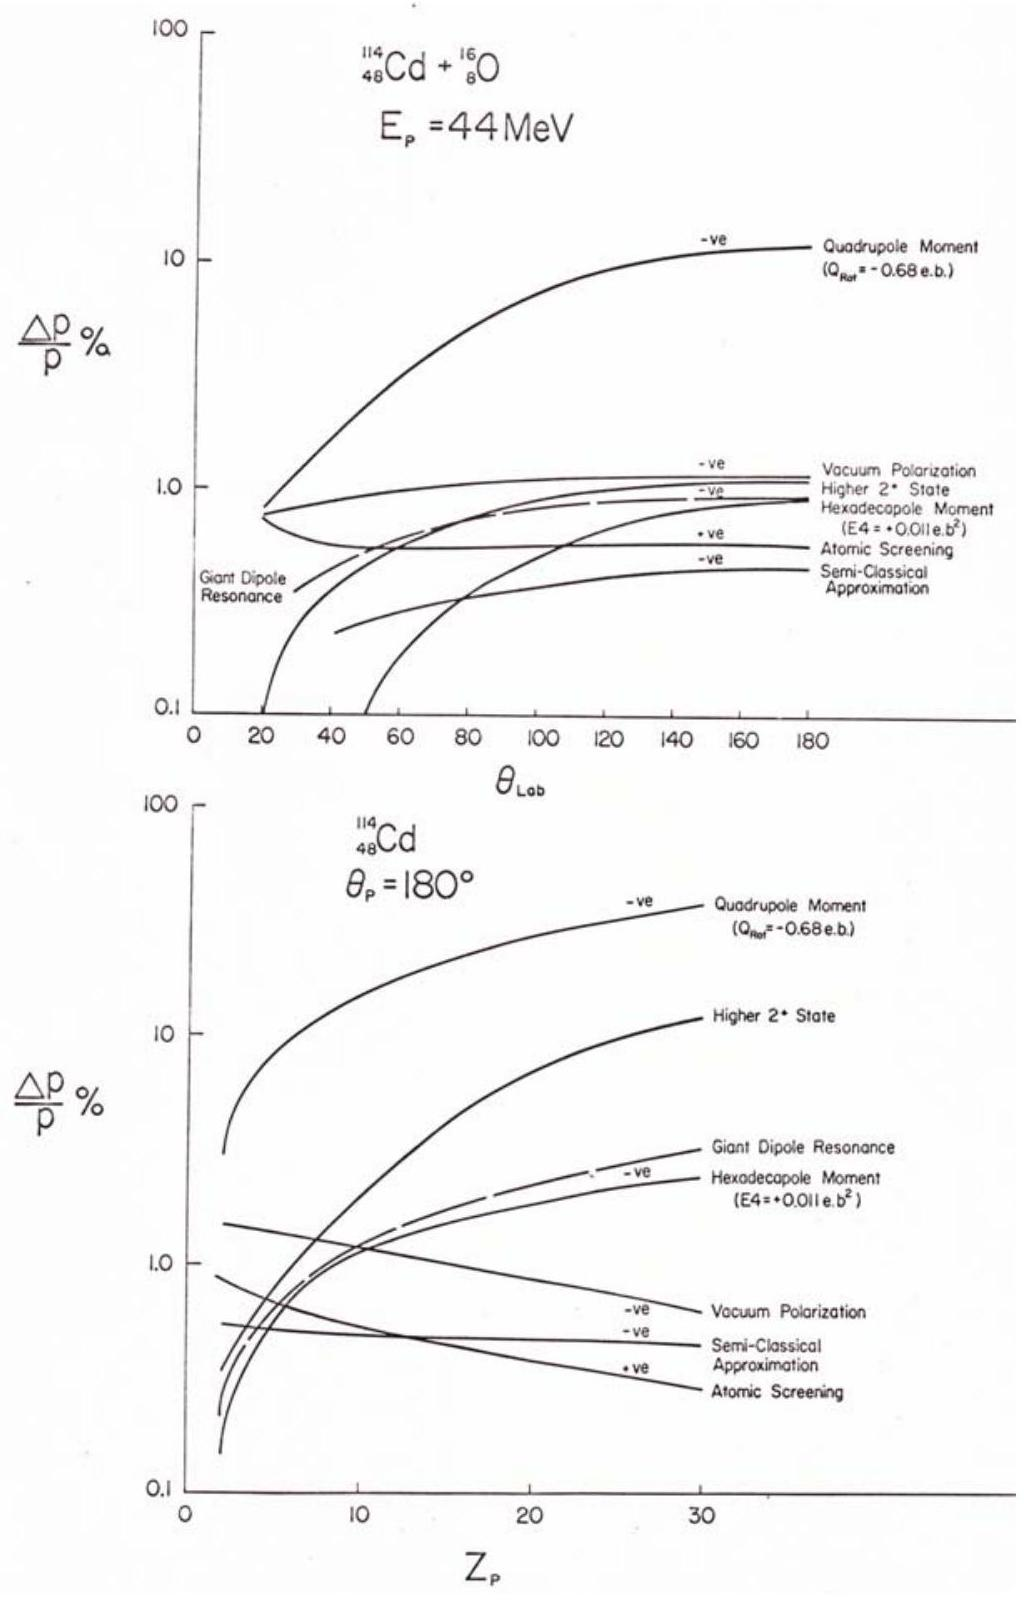
\includegraphics[max width=\textwidth, center]{2025_02_07_204a351db2d7f48b61ebg-026}

Figure 2.8: The importance of several effects on Coulomb excitation of the first excited $2_{1}^{+}$state in ${ }^{114} C d$. The ordinate gives the $\%$ change in excited state excitation probability as a function of scattering angle (upper) and projectile $Z_{p}$ (lower).\\
than the reorientation effect. Note that virtual excitation plus deexcitation $\gamma$-ray feeding involving higherlying states, which are not included in Figure 2.8, will be large for heavy-ion induced Coulomb excitation at bombarding energies near the safe energy. The large uncertainty due to virtual excitation of higher-lying states can be suppressed by using bombarding energies well below the safe energy to minimize multistep excitation processes. Note that measurement of the scattering-angle dependence of the Coulomb excitation probability is a more reliable and efficient way to study the reorientation effect since the scattering angle can be measured simultaneously eliminating problems associated with knowledge of the exact beam flux and bombarding energy.

For a prolate deformed rotor the intrinsic quadrupole moment is positive, whereas for states built on the band head rotation of the prolate rotor results in an oblate average shape having a negative static quadrupole moment leading to a negative contribution of the reorientation effect. In contrast the band-head of a $K^{\pi}=2^{+}$band of a prolately-deformed nucleus has a positive static quadrupole moment leading to a positive contribution to the excitation probability. As illustrated in figure 2.1, reorientation measurements are sensitive to destructive Coulomb-nuclear interference which mimics the reorientation effect and led to the safe bombarding energy given by equation 2.1 [CLI69,LES72].

\subsection*{2.3.3 Static $M 1$ moments}
Nuclear magnetic moments are a precise probe of the single-particle composition of nuclear states. Unfortunately Coulomb excitation process using bombarding energies below the Coulomb barrier is not sensitive to M1 static moments. However, the magnetic interaction between the magnetic dipole moments of the excited nuclear states and the $\sim 10^{4} T$ atomic hyperfine magnetic fields produce the dominant hyperfine interaction responsible for the deorientation effect that greatly perturbs the $p-\gamma$ angular correlations. If this atomic hyperfine magnetic field could be predicted accurately then the deorientation effect would provide a powerful probe for measuring the magnitude of the magnetic dipole moments of excited nuclear states. Unfortunately the atomic hyperfine fields involve complicated stochastic processes that currently cannot be predicted. Recent work has revived interest in use of the deorientation effect to measure magnetic moments of excited states in exotic nuclei[STO05]. The current version of GOSIA uses the two-state model with a common $g$-factor for all states. When a computer code becomes available that can accurately predict hyperfine fields, then it will be incorporated into GOSIA in order to directly fit static magnetic moments to measured $p-\gamma$ angular correlations following Coulomb excitation. This will provide the capability to simultaneously measure the $E \lambda$ modes, which determine the collective degrees of freedom, and the $M 1$ static moments that probe the shell structure.

\subsection*{2.3.4 Rotational invariants}
The rotational invariant method provides a powerful and elegant way to project the collective degrees of freedom from Coulomb excitation data. It is especially useful when both vibrational and rotational degrees of freedom are applicable. However, the lack of completeness in evaluation of the rotational invariants results in them not having the precision available from a detailed comparison of measured with theoretical matrix elements. Thus, for strongly-deformed nuclei, it usually is more profitable to make a detailed comparison of measured electromagnetic matrix elements directly with model predictions.

As discussed in chapter 9, evaluation of higher moments of the rotational invariants, such as the vibrational widths, requires data recorded over both scattering angle and a wide range of $Z$ values for the exciting nucleus. Note that the many coupled-channels in heavy-ion induced Coulomb excitation involve the same products of matrix elements as occur in evaluating the rotational invariants. The difference is that for Coulomb excitation the products are multiplied by kinematic factors due to the Coulomb excitation process. As a consequence, the errors assigned to the rotational invariants by GOSIA will be less than those obtained by combination of the errors of individual matrix elements assigned matrix elements without including the strong cross correlations. The sum-rule identities, plus common sense should be used in selecting which rotational invariants calculated by the rotational-invariants code SIGMA are meaningful.

\subsection*{2.4 Extraction of $E \lambda$ matrix elements from Coulomb excitation data}
\subsection*{2.4.1 Model independent analysis}
As discussed in chapter 1, the motivation for development of Gosia was to implement the capability to extract measured $E \lambda$ matrix elements model-independently from Coulomb excitation data. The first major task required to achieve this goal was to design experiments covering a wide dynamic range of Coulomb excitation strength that provide sufficient experimental data to overdetermine the many unknown matrix elements. Experimental techniques were developed to achieve this requirement in the 1980's and primarily involved Coulomb excitation measurements over a wide range of both scattering angle and $Z$ value of the unexcited nucleus. The second major task was the development of Gosia to model-independently extract the matrix elements via a least-squares search of the data. During the 1980's and early 1990's the ready availability of beam time at heavy-ion accelerator facilities, the availability of high-efficiency $p-\gamma$ detector facilities, and access to fast computer systems needed for the Gosia least-squares searches, enabled the first model-independent extraction of $E \lambda$ matrix elements from multiple Coulomb excitation data. These fairly complete sets of $E 2$ matrix elements made it possible to exploit the rotational invariants technique to extract the underlying quadrupole collective degrees of freedom directly from the Coulomb excitation data. Note that it is not viable to perform a completely model-independent analysis in that models are required to extrapolate from the set of measured $E \lambda$ matrix elements to estimate other matrix elements that are insensitive to the data set but play a weak role in the Coulomb excitation process. For example, the influence of virtual excitation of the highest spin states or of excited-state static electric quadrupole moments.

\subsection*{2.4.2 Model dependent analyses}
The much improved sensitivity provided by modern $4 \pi$ high-resolution $\gamma$-ray detector facilities, such as Gammasphere when coupled to $4 \pi$ recoil-ion detectors like CHICO, has greatly expanded the number of collective bands and levels observed in heavy-ion induced Coulomb excitation measurements. Since the late 1990 ' $s$ this improved sensitivity has led to an explosive increase in the number of $E \lambda$ matrix elements involved in least-squares fits to Coulomb excitation data. For example, current heavy-ion induced Coulomb excitation measurements of an odd-A actinide, strongly-deformed, nucleus can populate $\approx 300$ levels in $\approx 12$ collective bands coupled by $\approx 3000 E \lambda$ matrix elements [WAR12, WAR12]. This rapid increase in the number of unknowns, and concomitant increase in the dimension of the least-squares search problem, coupled with a reduction in available beam time due to closure of a substantial fraction of the arsenal of heavy-ion accelerator facilities, has made it no longer viable to obtain sufficiently complete sets of Coulomb excitation data for a full model-independent Gosia analysis. Fortunately the collective correlations are strong for low-lying spectra of most nuclei making it viable to exploit these collective correlations to greatly reduce the number of fitted parameters to accommodate the smaller data sets. For example, for the axially-symmetric rigid rotor the fit to the diagonal and transition $E 2$ matrix elements can be reduced to fitting the one intrinsic quadrupole moment of the band, which, in principle, only requires measurement of one $E 2$ matrix element. Thus model-dependent analyses of Coulomb excitation data can be used to extract the relevant physics even when the data set is insufficient to overdetermine the many unknown matrix elements model independently.

A model-dependent approach that has been highly successfully involves factoring the system into subgroups of levels that have similar collective correlations, and assuming that a model can adequately relate the $E \lambda$ matrix elements for each of these localized subgroups of levels. That is, the model is used to relate the $E \lambda$ matrix elements in a localized region by coupling all of the "dependents" to one "master" member of the subgroup. The least-squares fit then is made to find the best values of the master matrix elements with the dependents varying in proportion to the masters. This approach can reduce the number of parameters being fit more than an order of magnitude. The best-fit values for these master matrix elements then can be used iteratively to refine the model-dependent coupling employed for correlating the matrix elements in the localized subgroups. As an example, in strongly-deformed nuclei the ground rotational band levels below the first band crossing can be broken into one or two subgroups each of which are coupled to common intrinsic $E 2$ moments, the levels above the band crossing also can be broken into similar subgroups, while the individual matrix elements around the band crossing can be treated as independent parameters. An iterative\\
procedure then can be employed where models are assumed to be sufficient accurate locally to extrapolate the measured sensitive matrix elements to model-dependently predict the less sensitive matrix elements.

The model-dependent approach must be treated with considerable care because the strong cross correlations can lead to erroneous conclusions. The fact that one model fits the experimental Coulomb excitation data is not a proof that this solution is unique. For example, the Davydov-Chaban rigid-triaxial rotor model reproduced well the measured Coulomb excitation yields for an early multiple Coulomb excitation studies of ${ }^{192,194,196} \mathrm{Pt}$ [LEE77] implying the existence of rigid triaxial deformation. A subsequent more extensive Coulomb excitation study,[WU83, WU96] that was analysed using Gosia, determined that these nuclei are very soft to $\beta$ and $\gamma$ vibrational degrees of freedom. The earlier erroneous conclusion that this nucleus behaved like a rigid triaxial rotor was fortuitous because the early measurements were sensitive only to the centroids of the $\beta$ and $\gamma$ shape degrees of freedom. Another example is that the axially-symmetric model often can give an almost equally acceptable fits to Coulomb excitation data of triaxially-deformed nuclei where erroneous $B(E 2)$ strengths compensate for incorrectly assumed static electric quadrupole moments. Thus it is important to compare the quality of model-dependent fits using various competing collective models to derive reliable conclusions as to the relative efficacy of different collective models.

\subsection*{2.4.3 Axially-symmetric rotational-band relations for $E \lambda$ matrix elements}
As mentioned above, Gosia and the GUI Rachel both incorporate the ability to couple the ratio of any $E \lambda$ matrix elements in order to reduce the number of fitted parameters which can be exploited to make model-dependent fits by setting the ratio of matrix elements to conform to any collective model. Gosia and Rachel both incorporate the ability to calculate the relative $E \lambda$ matrix elements using three simple collective models that assume axially-symmetric rotation to facilitate preparing initial inputs to Gosia and to use for calculating the coupling often used to fit localized subsets of collective variables to the Coulomb excitation data set. Currently Gosia and Rachel incorporate the ability to generate $E 2$ matrix elements using the Alaga rules (equations 2.6, 2.8), Mikhailov $K$-band mixing (equation 2.13 ), and $K$-forbidden transitions (equation 2.11) for axially-symmetric rotational nuclei. Note that Gosia is not necessarily restricted to these simple models.

\section*{Spin-independent intrinsic moments}
$K$-allowed transitions; If the intrinsic frame electric matrix elements are spin independent, then the reduced matrix elements between states of spin $I$ with component $K$ along the symmetry axis for axiallysymmetric rotational-band structure are related by the following relations [BOH69]


\begin{equation*}
\left\langle K_{2} I_{2}\|M(\lambda)\| K_{1} I_{1}\right\rangle=\sqrt{\left(2 I_{1}+1\right)}\binom{\left\langle I_{1} K_{1} \lambda K_{2}-K_{1} \mid I_{2} K_{2}\right\rangle\left\langle K_{2}\right| M\left(\lambda, \nu=K_{2}-K_{1}\right)\left|K_{1}\right\rangle}{+(-1)^{I_{1}+K_{1}}\left\langle I_{1}-K_{1} \lambda K_{2}+K_{1} \mid I_{2} K_{2}\right\rangle\left\langle K_{2}\right| M\left(\lambda, \nu=K_{2}+K_{1}\right)\left|\bar{K}_{1}\right\rangle} \tag{2.5}
\end{equation*}


for $K_{1} \neq 0, K_{2} \neq 0$.\\
If either one of the bands has $K=0$, then the first term in equation 2.5 is equal to the second "signaturedependent" term and thus equation 2.5 reduces to


\begin{equation*}
\left\langle K_{2} I_{2}\|M(\lambda)\| K_{1}=0, I_{1}\right\rangle=\sqrt{\left(2 I_{1}+1\right)}\left\langle I_{1} 0 \lambda K_{2} \mid I_{2} K_{2}\right\rangle\left\langle K_{2}\right| M\left(\lambda, \nu=K_{2}\right)|0\rangle \xi \tag{2.6}
\end{equation*}


where $\xi=\sqrt{2}$ if $K_{2} \neq 0$ and $\xi=1$ if $K_{2}=0$. Note that the intrinsic matrix element within a $K=0$ band $\left\langle K_{2}\right| M(\lambda, \nu=0)|0\rangle=0$ if $M(\lambda, \nu=0)$ is odd under time reversal combined with Hermitian conjugation.

For the special case of the $E 2$ operator the intrinsic matrix element of an axially-symmetric rotor can be defined in terms of an intrinsic quadrupole moment $e Q_{0}$ where


\begin{equation*}
e Q_{0} \equiv \sqrt{\frac{16 \pi}{5}}\langle K| M(\lambda, \nu=0)|K\rangle \tag{2.7}
\end{equation*}


Then for a single collective band, with a component of the angular momentum along the symmetry axis $K$, the reduced $E 2$ matrix element can be written in terms of the intrinsic quadrupole moment $Q_{0}$ as


\begin{equation*}
\left\langle K I_{2}\|M(E 2)\| K I_{1}\right\rangle=\sqrt{\left(2 I_{1}+1\right)}\left\langle I_{1} K, 2,0 \mid I_{2} K\right\rangle \sqrt{\frac{5}{16 \pi}} e Q_{0} \tag{2.8}
\end{equation*}


The $E 2$ transition strength is related by


\begin{equation*}
B\left(E 2 ; K I_{1} \rightarrow K I_{2}\right)=\frac{5}{16 \pi} e^{2} Q_{0}^{2}\left\langle I_{1} K, 2,0 \mid I_{2} K\right\rangle^{2} \tag{2.9}
\end{equation*}


while the static $E 2$ moment $Q$ is related by


\begin{align*}
Q & =\langle I K 20 \mid I K\rangle\langle I I 20 \mid I I\rangle Q_{0}  \tag{2.10}\\
& =\frac{3 K^{2}-I(I+1)}{(I+1)(2 I+3)} Q_{0}
\end{align*}


The $I$ dependence of matrix elements $2.5,2.6$ are of a simple geometric nature reflecting the differing orientation angles for the different members of the rotational band. These geometric relations are frequently referred to as the Alaga rules.\\
$K$-forbidden transitions Transitions for which $\left|K_{2}-K_{1}\right|>\lambda$ are $K$-forbidden as given by equations $2.5,2.6$ which are zero due to the Clebsch-Gordan triangle rule not being obeyed. The order of the $K$ forbiddenness, $n$, is defined by

$$
n \equiv\left|K_{2}-K_{1}\right|-\lambda
$$

Equation 4.95 in [BOH69] gives that the $K$ forbidden matrix element is given by\\
$\left\langle K_{2} I_{2}\|M(\lambda)\| K_{1}, I_{1}\right\rangle=\sqrt{\left(2 I_{1}+1\right)}\left\langle I_{1}, K_{2}-\lambda, \lambda, \lambda \mid I_{2} K_{2}\right\rangle \sqrt{\frac{\left(I_{1}-K_{1}\right)!\left(I_{1}+K_{1}+n\right)!}{\left(I_{1}-K_{1}-n\right)!\left(I_{1}+K_{1}\right)!}}\left\langle K_{2}\right| m_{\Delta K=\lambda+n, \nu=\lambda}\left|K_{1}\right\rangle \xi$\\
where $K_{2}=K_{1}+\lambda+n$ and assuming that $K_{2}>K_{1}$. The parameter $\xi=\sqrt{2}$ if $K_{1}=0$ and $\xi=1$ if $K_{1} \neq 0$.

\section*{Spin-dependent intrinsic moments}
The assumption that the intrinsic matrix elements are spin independent is approximately valid only under limited conditions. At high angular momentum the Coriolis and centrifugal effects distort both the nuclear shape and microscopic structure leading to band mixing. The microscopic structure underlying rotational band behaviour in nuclei implies limits to the maximum angular moment for any set of valence nucleons. When the angular momentum approaches the maximum possible from full alignment of the valence nucleons this leads to band termination and a dramatic reduction in the collectivity near the terminating angular momentum. The functional form of the spin dependence of the intrinsic frame matrix elements can be incorporated as additional parameters in model-dependent analysis of Coulomb excitation data to take into account the underlying microscopic structure or the impact of rotationally-induced stress.

\section*{$K$-band mixing}
In the rotating frame the Coriolis force leads to particle-rotation coupling term in the Hamiltonian of the form

$$
H_{c o r}=\frac{\hbar^{2}}{2 \Im_{0}}\left(j_{+} I_{-}+j_{-} I_{+}\right)
$$

This term is non-diagonal in $K$ coupling of the intrinsic and rotational motion with $\Delta K= \pm 1$. Second-order Coriolis coupling leads to $\Delta K=2$ coupling which is an important contributor to $K$-band mixing. The interband $E 2$ matrix elements provide a sensitive probe of $K$-band mixing. Equation $4-210$ in reference [BOH69] gives that the interband $\Delta K=2 E 2$ matrix element equals


\begin{equation*}
\left\langle K_{2}=K_{1}+2, I_{2}\|M(E 2)\| K_{1} I_{1}\right\rangle=\sqrt{\left(2 I_{1}+1\right)}\left\langle I_{1} K_{1}, 2,2 \mid I_{2} K_{2}\right\rangle\left(M_{1}+M_{2}\left(I_{2}\left(I_{2}+1\right)-I_{1}\left(I_{1}+1\right)\right)\right) \xi \tag{2.12}
\end{equation*}


where $\xi=\sqrt{2}$ if $K_{1}=0$ and $\xi=1$ if $K_{1} \neq 0$ and


\begin{align*}
& M_{1}=\left\langle K_{2}\right| M(\lambda, \nu=2)\left|K_{1}\right\rangle-4\left(K_{1}+1\right) M_{2}  \tag{2.13}\\
& M_{2}=\sqrt{\left(\frac{15}{8 \pi}\right)} e Q_{0}\left\langle K_{2}\right| \varepsilon_{+2}\left|K_{1}\right\rangle=\sqrt{\left(\frac{15}{8 \pi}\right)} e Q_{0} \frac{\left\langle K_{2}\right| h_{+2}\left|K_{1}\right\rangle}{E\left(K_{2}\right)-E\left(K_{1}\right)}
\end{align*}


$M_{1}$ and $M_{2}$ are the Mikhailov intrinsic matrix elements that can be fit to the data. This Mikhailov expansion of the $\Delta K=2$ mixing is a useful model for correlating weak $K$-mixing in strongly-deformed nuclei.

\subsection*{2.4.4 Model-dependent fits using more general Hamiltonians}
Any phenomenological macroscopic or microscopic models of nuclear structure can be employed to relate $E \lambda$ or $M \lambda$ matrix elements for use in model-dependent fits to Coulomb excitation data as described above. The axially-symmetric rotor model has only limited validity to the yrast domain of strongly-deformed heavy nuclei. General collective Hamiltonians, that include both triaxial and vibrational degrees of freedom, are required to usefully describe collective correlations in most nuclei. Triaxial quadrupole collective degrees of freedom lead to large $K$-mixing that is best represented by use of a non-axial deformed collective model, where the large $K$-mixing is built into the basis states, while vibrational degrees of freedom lead to strong spin dependence of the intrinsic frame collective-model parameters. The complete Bohr collective-model Hamiltonian for quadrupole collectivity can be used to describe collective correlations in such nuclei. Note that Coulomb excitation work has shown that the quasi-rotational features of the Bohr Hamiltonian are a more useful representation of quadrupole rotation-vibration collective motion in shape transitional nuclei than the use of harmonic phonon bases.

\subsection*{2.5 Test of Coulomb excitation theory}
It is important to verify experimentally the accuracy of the Coulomb excitation methods used. One accurate test of Coulomb excitation is the $B\left(E 2 ; 0^{+} \rightarrow 2_{1}^{+}\right)$in ${ }^{60} \mathrm{Ni}$ where the Coulomb excitation [LES74] and resonance fluorescence [MET70] results agree to $1 \pm 2 \%$. The recoil distance technique was used to measure the lifetimes[KOT89] of eight low-lying states in ${ }^{110} \mathrm{Pd}$ to check, in an unambiguous way, the results of earlier Coulomb excitation results [HAS80] analyzed using the GOSIA code. The recoil distance lifetimes are in excellent agreement with the lifetimes calculated from the Coulomb excitation work, i.e. a weighted mean difference of $2.2 \pm 3.5 \%$. This confirms that the Coulomb excitation analysis procedure introduces no major systematic errors even for the very complicated case of ${ }^{110} \mathrm{Pd}$. Agreement at the $5-10 \%$ level has been found from comparisons of Coulomb excitation and recoil distance or Doppler-shift attenuation measurements of the $B(E 2)$ values for the ground bands of many nuclei [GUI76, WAR76]. Coulomb excitation[VER74] of ${ }^{7} \mathrm{Li}$ by ${ }^{208} \mathrm{~Pb}$ and ${ }^{138} \mathrm{Ba}$ gave a value of the static moment for the ${ }^{7} \mathrm{Li}$ ground state of $Q_{3 / 2}=-4.0 \pm 1.1 e \cdot f m^{2}$ to be compared with the molecular beam spectroscopy value[GRE72] of $3.66 \pm 0.03 e \cdot \mathrm{fm}^{2}$. These tests support the validity of the techniques used to analyze Coulomb excitation data.

\subsection*{2.6 Simulation of planned experiments}
The time, effort and cost involved in performing and analyzing a multiple-Coulomb excitation experiment warrants thorough prior planning. GOSIA is ideally suited to performing simulations of planned experiments to identify sensitivity and potential problems. GOSIA, coupled to the GUI RACHEL, can use collective models to generate complete sets of matrix elements that can be used in simulation calculations of Coulomb excitation $p-\gamma$ yields. RACHEL can modify these calculated yields to include random statistical error to provide a good input data set for a least-squares search using GOSIA. The test data set also can include simulated lifetimes, branching ratios, etc. The results of such fits to simulated data give the most reliable measure of the sensitivity and the correlated errors that can be expected from planned experiments. These can be of considerable value for optimizing the planned experiment to achieve the scientific goals with the highest overall efficiency. Unanticipated problems encountered during the experiment or data analysis can be minimized by careful simulations and planning. The following are questions and issues that need to be considered when planning an experiment:

\begin{itemize}
  \item Bombarding energy: Is it low enough to ensure that complicated and time-consuming Coulombnuclear calculations are unnecessary, and yet high enough to ensure that the cross sections are sufficient to provide adequate statistical accurate data? What will be the systematic error in the measured energy of the incident beam?
  \item Sensitivity: Does the adiabaticity and eccentricity approach the limits of the numerical accuracy of GOSIA?
  \item Target thickness: Is the target thickness sufficient for obtain good statistics data and yet thin enough to provide for adequate recoil-ion detection and resolution? What will be the accuracy and non-uniformity of the target thickness, including the impact of target sputtering etc, on the experiment?
  \item Heavy-ion detection: Are the angle, time, and energy resolution of the particle detectors sufficient to separate the kinematic solutions? Are the thresholds for recoil detection adequate for the ions of interest? Are the predicted count rates within the detector and data acquisition system limitations?
  \item Gamma-ray detection: Are the angular resolution and segmentation of both the recoil-ion detector and the gamma-detector arrays sufficient to obtain adequate $\gamma$-ray energy resolution, after Dopplercorrection? Is the detector efficiency sufficient to exploit the much higher sensitivity provided by good statistics high-fold $\gamma$-ray coincident data? What will be the sensitivity of the data to $p-\gamma$ angular correlations and the deorientation effect? Is the time resolution adequate? Are absorbers required to suppress x-ray background from the target? Is radiation shielding adequate? What is the $\gamma$-ray detection efficiency for delayed $\gamma$-ray decay by recoils that are displaced from the target position or stopped in the recoil-ion detector?
  \item Absolute cross sections: What reference will be used to provide absolute normalization of the data (e.g. particle singles, known reference $B(E \lambda)$ values in either of the interacting nuclei, the yield for low-lying transitions in the ground band)? What is the accuracy for knowing the exact geometry, angles and energy thresholds of the recoil-ion detectors? What is the accuracy of the measured peak detection efficiency of the gamma-detector array? Typically the error in the absolute detection efficiency is the order of $5 \%$.
  \item Data acquisition: Can the data acquisition system handle the count rate? What are the dead-times due to pile-up, count rate, etc? What is the time resolution, time range and time calibration for recording delayed $\gamma$-ray deexcitation? An on-line data analysis program that displays coincident $\gamma$-ray spectra, Doppler-corrected for deexcitation by either reaction product, is important for monitoring during data acquisition.
  \item Data analysis: The Coulomb excitation calculations must include sufficient higher-spin states beyond those observed to account for virtual excitation effects. Generate a starting set of matrix elements that has a logical phase convention to facilitate comparison with collective models. Accurate branching ratio data can trap the least-squares search in one relative phase difference between matrix elements of the branch. For such cases it is necessary to either switch off the branching ratio data or manually change one of the phases. The uniqueness of the measured matrix elements can be tested by using different sets of starting matrix elements. Estimation of the correlated errors for the strongly-coupled equations in multiple Coulomb excitation is a non-trivial procedure. Typically the correlated errors are more than twice the diagonal errors.
\end{itemize}

\section*{Chapter 3}
\section*{Semiclassical theory}


\subsection*{3.1 Semiclassical approach}
The semiclassical theory of Coulomb excitation is discussed in the Alder-Winther monograph on the subject [ALD75]. This reference presents alternative approaches to the formal description of electromagnetic excitation which are valuable for better understanding the nature of the processes in question, but they are not viable practically. Therefore, the following outline of Coulomb excitation theory is limited to the formalism actually used in the code. Particularly, the differences between the semiclassical and the fully quantal descriptions will not be discussed. Perturbation approaches are not useful for multiple Coulomb excitation and thus less attention will be given to such perturbation methods.

As illustrated in figure 2.4, the effective collision time is of the order of $3 \times 10^{-21} \mathrm{sec}$, which is $10^{8}$ times shorter than the typical lifetimes for $\gamma$-ray deexcitation of the nuclear states involved in Coulomb excitation. This allows the excitation and subsequent $\gamma$ decay to be treated as separate and sequential processes. Finally, using the expansion of the electromagnetic interaction potential in a multipole series [BOH69] allows a representation of this potential in terms of a sum of three factors: a monopole-monopole interaction, defining the kinematics only; a mutual monopole-multipole interaction and a mutual multipolemultipole interaction. The third term is weak compared to the monopole-multipole term and, within the desired accuracy, can be neglected since it does not interfere with the monopole-multipole terms. This treatment yields a convenient separation of the Schrödinger equation, i.e., the excitation of both projectile and target can be independently expressed as:


\begin{equation*}
i h \frac{\delta}{\delta t}\left|\psi_{1,2}>=\left(H_{1,2}^{o}+V_{1,2}(\bar{r}(t))\right)\right| \psi_{1,2}> \tag{3.1}
\end{equation*}


where $V_{1,2}(\bar{r}(t))$ stands for monopole-multipole interaction between unexcited nucleus (monopole) and excited nucleus (multipole) - indexed by 1 - or vice versa, indexed by 2 . The monopole-monopole interaction $H_{1,2}^{0}$ determines the time-dependence of the potential by the classical trajectory $\bar{r}(t)$. As can be seen, target and projectile nuclei can be interchanged, therefore the indices 1 and 2 are used only where the distinction is necessary.

\subsection*{3.2 Electromagnetic interaction}
To solve the time-dependent Schrödinger equation 3.1 we represent $\mid \psi(\bar{r}, t)>$ as a linear combination of the free-nucleus wave functions $\phi(\bar{r})$, taken with time-dependent coefficients of the form:


\begin{equation*}
\left|\psi(\bar{r}, t)>=\sum_{n} a_{n}(t)\right| \Phi_{n}(\bar{r})>\exp \left(-i E_{n} t / \hbar\right) \tag{3.2}
\end{equation*}


with

$$
H^{o}\left|\Phi_{n}>=E_{n}\right| \Phi_{n}>
$$

Substituting 3.2 in 3.1 gives:


\begin{equation*}
i \hbar \sum_{n} \frac{d a_{n}(t)}{d t}\left|\Phi_{n}(\bar{r})>\exp \left(-i E_{n} t / \hbar\right)=\sum_{n} a_{n}(t) V(t)\right| \Phi_{n}(\bar{r})>\exp \left(-i E_{n} t / \hbar\right) \tag{3.3}
\end{equation*}


Taking into account orthonormality of the free nucleus wavefunctions $\left|\Phi_{n}\right\rangle,\left(\left\langle\Phi_{k} \mid \Phi_{n}\right\rangle=\delta_{k n}\right)$ gives:


\begin{equation*}
\frac{d a_{k}(t)}{d t}=-\frac{i}{\hbar} \sum_{n} a_{n}(t)<\Phi_{k}|V(t)| \Phi_{n}>\exp \frac{i t}{\hbar}\left(E_{k}-E_{n}\right) \tag{3.4}
\end{equation*}


The system of differential equations 3.4 defines the complex expansion coefficients $a_{k}(t)$. Before the collision, the nucleus is assumed to be in the initial state which usually is the ground state, thus the initial condition (corresponding to $t=-\infty$ ) can be expressed as $a_{k}=\delta_{k, 0}$, where index $O$ stands for ground state. The nucleus after the collision is then described by the set of excitation amplitudes $a_{k}(t=\infty)$ defining excitation probabilities where $P_{k}=a_{k} a_{k}^{*}$, as follows from 3.2. As mentioned above, the interaction potential $V(t)$ can be expanded into a multipole series:


\begin{equation*}
V_{1,2}(t)=\sum_{\lambda=1}^{\infty} \sum_{\mu=-\lambda}^{\lambda} \frac{4 \pi Z_{2,1} e}{2 \lambda+1}(-1)^{\mu} S_{\lambda \mu}(t) M_{1,2}(\lambda,-\mu) \tag{3.5}
\end{equation*}


where


\begin{equation*}
S_{\lambda \mu}(t)=\frac{Y_{\lambda \mu}(\theta(t), \phi(t))}{[r(t)]^{\lambda+1}} \tag{3.6}
\end{equation*}


for electric excitation and


\begin{equation*}
S_{\lambda \mu}(t)=\frac{1}{c \cdot \lambda} \frac{\frac{d \bar{r}}{d t} \cdot(\bar{r} \times \bar{\nabla})}{[r(t)]^{\lambda+1}} Y_{\lambda \mu}(\theta(t), \phi(t)) \tag{3.7}
\end{equation*}


for magnetic excitation. Note that $Y_{\lambda \mu}$ denotes standard normalized spherical harmonics. The symbol $M(\lambda, \mu)$ stands for electric and magnetic multipole moments, as defined in [BOH69] :


\begin{gather*}
M(E \lambda, \mu)=\int \rho(\bar{r}) r^{\lambda} Y_{\lambda \mu}(\theta, \phi) d^{3} \bar{r}  \tag{3.8}\\
M(M \lambda, \mu)=\frac{1}{c(\lambda+1)} \int r^{\lambda} \bar{j}(\bar{r})(\bar{r} \times \bar{\nabla}) Y_{\lambda \mu}(\theta, \phi) d^{3} \bar{r} \tag{3.9}
\end{gather*}


$\rho(\bar{r})$ and $\bar{j}(\bar{r})$ being spatial charge and current distributions of a free nucleus respectively. Inserting 3.5-3.9 into 3.4 one obtains the parametrization of electromagnetic excitation by the matrix elements of multipole moment operators:


\begin{equation*}
\left.\frac{d a_{k}(t)}{d t}=-i \frac{4 \pi Z_{1,2} e}{\hbar} \sum_{n} a_{n}(t) \exp \frac{i t}{\hbar}\left(E_{k}-E_{n}\right) \sum_{\lambda \mu}(-1)^{\mu} \cdot S_{\lambda \mu}(t)<\Phi_{k}|M(\lambda,-\mu)| \Phi_{n}\right\rangle \tag{3.10}
\end{equation*}


\subsection*{3.3 Coordinate frame}
To express the time-dependent functions $S_{\lambda \mu}(t)$ it is convenient to introduce a frame of coordinates with the $z$-axis along the symmetry axis of the incoming particle trajectory and $y$-axis in the trajectory plane defined in such a way that the incoming particle velocity component $v_{y}$ is positive. The $x$-axis then is defined to form a right-handed cartesian system of coordinates (Fig. 3.1).

In this system of coordinates, one can describe the relative two-body motion, treated as the classical hyperbolic Kepler solution, introducing two parameters $\epsilon$ and $\omega$. The parameter $\epsilon$, called the orbit eccentricity, is expressed by the center-of-mass scattering angle $\theta_{c m}$ :\\
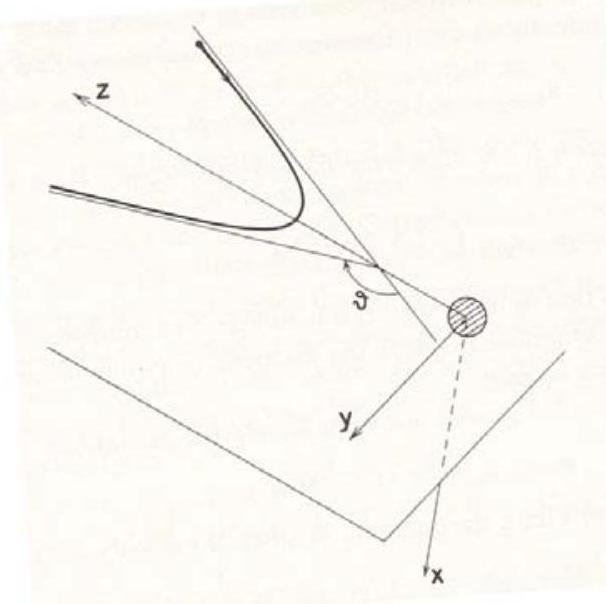
\includegraphics[max width=\textwidth, center]{2025_02_07_204a351db2d7f48b61ebg-035}

Figure 3.1: Coordinate system used to evaluate the Coulomb excitation amplitudes. The origin is chosen in the center of mass of the target nucleus. The $x$-axis is perpendicular to the plane of the orbit, the $z$-axis is along the symmetry axis of the incoming projectile orbit pointing towards the projectile, while the $y$-axis is chosen such that the $y$-component of the projectile velocity is positive. The scattering angle $\theta$ of the projectile is shown. Note that Alder and Winther [ALD75] call this coordinate system B.


\begin{equation*}
\epsilon=\frac{1}{\sin \frac{\theta_{c m}}{2}} \tag{3.11}
\end{equation*}


The dimensionless orbit parameter $\omega$, which replaces time, is given by:


\begin{equation*}
t=\frac{a}{v_{I}}(\epsilon \sinh \omega+\omega) \tag{3.12}
\end{equation*}


where $a=\frac{b}{2}$ is half the distance of closest approach for a head-on collision. This parametrization yields the following expression for the length of the radius-vector $\bar{r}$ :


\begin{equation*}
r=a(\epsilon \cosh \omega+1) \tag{3.13}
\end{equation*}


Explicitly, the Cartesian coordinates are expressed in terms of $\epsilon$ and $\omega$ as:


\begin{align*}
x & =0  \tag{3.14}\\
y & =a\left(\epsilon^{2}-1\right)^{1 / 2} \sinh \omega \\
z & =a(\cosh \omega+\epsilon)
\end{align*}


Note that the closest approach corresponds to $\omega=0$.\\
The functions $S(t)$ are replaced by dimensionless "collision functions" $Q(\epsilon, \omega)$ :


\begin{equation*}
Q_{\lambda, \mu}^{E}(\epsilon, \omega)=a^{\lambda} \frac{(2 \lambda-1)!!}{(\lambda-1)!}\left(\frac{\pi}{2 \lambda+1}\right)^{1 / 2} r(\omega) S_{\lambda, \mu}^{E}(t(\omega)) \tag{3.15}
\end{equation*}


for electric excitations, and


\begin{equation*}
Q_{\lambda, \mu}^{M}(\epsilon, \omega)=\frac{c}{v} a^{\lambda} \frac{(2 \lambda-1)!!}{(\lambda-1)!}\left(\frac{\pi}{2 \lambda+1}\right)^{1 / 2} r(\omega) S_{\lambda, \mu}^{M}(t(\omega)) \tag{3.16}
\end{equation*}


for magnetic excitations. The explicit expressions for the collision functions $Q(\varepsilon, \omega)$ for $E 1$ to $E 6$ and $M 1$, $M 2$ are compiled in Table 3.1.

It is convenient to replace the multipole operator matrix elements $<I_{s} M_{s}|M(\lambda, \mu)| I_{f} M_{f}>$ by reduced matrix elements $<I_{s} \| M(\lambda)| | I_{f}>$ using the Wigner-Eckart theorem:

\[
<I_{s} M_{s}|M(\lambda, \mu)| I_{f} M_{f}>=(-1)^{I_{s}-M_{s}}\left(\begin{array}{ccc}
I_{s} & \lambda & I_{f}  \tag{3.17}\\
-M_{s} & \mu & M_{f}
\end{array}\right)<I_{s}\|M(\lambda)\| I_{f}>
\]

where $\left(\begin{array}{ccc}I_{s} & \lambda & I_{f} \\ -M_{s} & \mu & M_{f}\end{array}\right)$ is the $3 j$ symbol. It is presumed that the phase convention for the wavefunctions $\mid I>$ is such that the reduced matrix elements are real.

\subsection*{3.4 Symmetrized Coulomb orbit}
The naive semiclassical description of Coulomb excitation neglects the energy loss of the recoiling ions for each final state due to inelastic excitation and the resultant modification of the trajectory. To first order, the effect of energy transfer can be approximated by symmetrization of relevant excitation parameters, i.e. taking an average of these parameters corresponding to perturbed and unperturbed orbits (see below). More accurate determination of energy transfer effects is not possible, since in the classical kinematics picture it is not known at which point of the trajectory that this transfer actually took place. Fortunately, in most cases the excitation energy for pure electromagnetic processes is a small fraction of the total bombarding energy, so the symmetrization procedure used is sufficiently accurate.

In first-order perturbation theory a systematic improvement to the semiclassical theory is obtained by a WKB treatment which suggests the use of the following symmetrized relations. The symmetrized orbit is characterized by a symmetrized half distance of closest approach defined by


\begin{equation*}
a_{k n}=\frac{Z_{1} Z_{2} e^{2}}{\mu v_{k} v_{n}} \tag{3.18}
\end{equation*}


where $\mu$ is the reduced mass. This is symmetric in the initial and final velocities. The main dependence of the cross section on the velocity enters through the symmetrized adiabaticity parameter $\xi_{k n}$ which is the difference in wavenumber between the initial and final states. This can be expressed as


\begin{equation*}
\xi_{k n}=\eta_{k}-\eta_{n}=\frac{Z_{1} Z_{2} e^{2}}{\hbar}\left(\frac{1}{v_{k}}-\frac{1}{v_{n}}\right) \tag{3.19}
\end{equation*}


The adiabaticity parameters have been symmetrized with respect to initial and final velocities in equation 3.19, that is, in a manner that does not violate unitarity and time reversal invariance.

\subsection*{3.5 Coupled differential equations}
Insertion of equations 3.11 through 3.19 into 3.10 yields the final system of differential equations for the excitation amplitudes $a_{k}$. The following formulae are given already in a numerical representation of physical constants, corresponding to energies in MeV , reduced electric multipole matrix elements in $e b^{\lambda / 2}$ and reduced magnetic multipole matrix elements in $\mu_{n} \cdot b^{(\lambda-1) / 2}, \mu_{n}$ being the nuclear magneton.


\begin{equation*}
\frac{d a_{k}}{d \omega}=-i \sum_{\lambda \mu n} Q_{\lambda \mu}(\epsilon, \omega) \zeta_{k n}^{(\lambda \mu)} \cdot<I_{k}\|M(\lambda)\| I_{n}>\cdot \exp \left(i \xi_{k n}(\epsilon \sinh \omega+\omega)\right) \cdot a_{n}(\omega) \tag{3.20}
\end{equation*}


The one-dimensional indexing of excitation amplitudes $a_{k}$ involves all magnetic substates of states $|I\rangle$, which from a point of view of a theory of electromagnetic excitation are treated as independent states. The symmetrized adiabaticity parameters $\xi_{k n}$, which represent the ratio of a measure of the collision time and the natural nuclear period for a transition, are given by:


\begin{gather*}
\xi_{k n}=\frac{Z_{1} Z_{2} \sqrt{A_{1}}}{6.34977}\left(\left(E_{p}-s E_{k}\right)^{-1 / 2}-\left(E_{p}-s E_{n}\right)^{-1 / 2}\right)  \tag{3.21}\\
s=\left(1+A_{1} / A_{2}\right) \tag{3.22}
\end{gather*}


$E_{p}$ being the bombarding energy. The above is valid for target excitation, while for projectile excitation indices 1 and 2 are to be interchanged.

The same symmetrization convention is equally valid for the coupling parameters $\zeta_{k n}^{(\lambda \mu)}$ given by:

\[
\zeta_{k n}^{(\lambda \mu)}=(2 \lambda+1)^{1 / 2}(-1)^{I_{n}-M_{n}}\left(\begin{array}{ccc}
I_{n} & \lambda & I_{k}  \tag{3.23}\\
-M_{n} & \mu & M_{k}
\end{array}\right) \psi_{k n}
\]

with


\begin{equation*}
\psi_{k n}=C_{\lambda}^{E(M)} \frac{Z_{1} \sqrt{A_{1}}}{\left(s Z_{1} Z_{2}\right)^{\lambda}}\left\{\left(E_{p}-s E_{k}\right)\left(E_{p}-s E_{n}\right)\right\}^{(2 \lambda-1) / 4} \tag{3.24}
\end{equation*}


where the numerical coefficients $C_{\lambda}^{E}(M)$ are different for electric and magnetic excitation and are given explicitly as:


\begin{gather*}
C_{\lambda}^{E}=1.116547 \cdot(13.889122)^{\lambda} \cdot \frac{(\lambda-1)!}{(2 \lambda+1)!!}  \tag{3.25}\\
C_{\lambda}^{M}=(v / c) C_{\lambda}^{E} / 95.0981942 \tag{3.26}
\end{gather*}


As pointed out in [ALD75], Appendix J, the electric dipole polarization effect can be approximately accounted for by modifying the collision functions corresponding to $E 2$ excitation:


\begin{equation*}
Q_{2 \mu}(\epsilon, \omega) \longrightarrow Q_{2 \mu}(\epsilon, \omega) \cdot\left(1-z \frac{a}{r}\right) \tag{3.27}
\end{equation*}


where


\begin{equation*}
z=d \cdot \frac{E_{p} A_{2}}{Z_{2}^{2}\left(1+A_{1} / A_{2}\right)} \tag{3.28}
\end{equation*}


$d$ being an adjustable empirical $E 1$ polarization strength. A widely accepted value is $d=0.005$ if the bombarding energy $E_{p}$ is in MeV . Equation 3.13 gives that $\frac{a}{r}$ can be written as:


\begin{equation*}
\frac{a}{r}=\frac{1}{\epsilon \cosh \omega+1} \tag{3.29}
\end{equation*}


The useful symmetry properties of $Q_{\lambda \mu}$ are the following:


\begin{equation*}
Q_{\lambda \mu}(\epsilon,-\omega)=Q_{\lambda \mu}^{*}(\epsilon, \omega) \tag{3.30}
\end{equation*}


and, for electric excitation:


\begin{align*}
Q_{\lambda \mu}(\epsilon, \omega) & =Q_{\lambda-\mu}(\epsilon, \omega)  \tag{3.31}\\
Q_{\lambda \mu}(\epsilon,-\omega) & =(-1)^{\mu} Q_{\lambda \mu}(\epsilon, \omega) \tag{3.32}
\end{align*}


while for magnetic excitation:


\begin{align*}
Q_{\lambda \mu}(\epsilon, \omega) & =-Q_{\lambda-\mu}(\epsilon, \omega)  \tag{3.33}\\
Q_{\lambda \mu}(\epsilon,-\omega) & =(-1)^{\mu+1} Q_{\lambda \mu}(\epsilon, \omega) \tag{3.34}
\end{align*}


It should be noted that, in the coordinate system used here (Fig. 3.1), for backscattering $\left(\theta_{c m}=180^{\circ}\right.$; $\epsilon=1$ ) all electric $Q^{E}$ values with $\mu \neq 0$ vanish, as well as all magnetic $Q^{M}$ values; therefore the magnetic quantum number is conserved. This is physically understandable, since the process along the $z$-axis cannot change the magnetic quantum number. The conservation of magnetic quantum number, exactly true for backscattering, is approximately valid for an arbitrary scattering angle due to the dominance of electric collision functions with $\mu=0$. The backscattering is important experimentally, providing the closest possible distance of approach of the nuclei taking part in the excitation process and therefore providing the maximum excitation probability available from Coulomb excitation.

The coefficients $\zeta$, which define coupling of the nuclear states, are dependent on $Z, A$ and energy of the projectile. It is interesting to elucidate the effect of using various beams on a given target, assuming the\\
maximum safe bombarding energy of the projectile given by 2.1. Neglecting symmetrization, one gets from 2.1 and 3.23 :


\begin{equation*}
\zeta \sim\left(\frac{Z_{1} A_{1} d}{s Z_{2}}\right)^{1 / 2}\left(\frac{1.44}{d}\right)^{\lambda} \tag{3.35}
\end{equation*}


where


\begin{equation*}
d=1.25\left(A_{1}^{1 / 3}+A_{2}^{1 / 3}\right)+5 \tag{3.36}
\end{equation*}


and $s$ is defined in 3.22. It can be seen, taking into account the correlation of $A_{1}$ and $Z_{1}$, that the coupling coefficients $\zeta$ are almost directly proportional to the charge number of a projectile. Consequently, going from lighter to heavier beams leads to excitation of a growing number of levels, while the number of matrix elements influencing the process increases even faster.

The product $\xi \in$ relates the collision time to the natural time period for a nuclear transition. Appreciable excitation of nuclear levels is most probable when the relative oscillation of their eigenfunctions is slow on the scale of the effective collision time. That is, when the Fourier transform of the electromagnetic impulse has significant probability at the transition energy. This implies that the Coulomb excitation cross sections generally increase with decreasing adiabaticity $\xi$. Taking into account that the excitation energy is small compared to the bombarding energy, expressed in MeV , and expanding 3.21 in a series, yields the approximation:


\begin{equation*}
\xi_{k n} \sim \frac{Z_{1} Z_{2} A_{1}^{\frac{1}{2}}}{12.65} \frac{E_{n-} E_{k}}{E_{p} \sqrt{E_{p}}} \tag{3.37}
\end{equation*}


Coulomb excitation is most probable for small transition energy differences in contrast to the deexcitation process, that is, the adiabaticity limits Coulomb excitation to a band of states within about an MeV above the yrast sequence. Increasing the bombarding energy of the projectile enhances the Coulomb excitation not only because of increased coupling parameters $\zeta$ but also because of decreased values of $\xi$.

\subsection*{3.6 Orbital integrals}
A convenient way to visualize the excitation process is to introduce so-called orbital integrals $R_{\lambda \mu}(\epsilon, \xi)$, defined as:


\begin{equation*}
R_{\lambda \mu}(\epsilon, \xi)=\int_{-\infty}^{\infty} Q_{\lambda \mu}(\epsilon, \omega) \exp (i \xi(\epsilon \sinh \omega+\omega)) d \omega \tag{3.38}
\end{equation*}


The orbital integrals $R$ directly determine the excitation amplitudes, provided that the first-order perturbation approach is applicable. Generally, the formal solution of 3.20 can be expressed by an infinite integral series as:


\begin{gather*}
\left.\left.\bar{a}(\omega=\infty)=\bar{a}_{o}+\left\{\int_{-\infty}^{\infty} A\left(\omega_{o}\right) d \omega_{o}\right)\right\} \bar{a}_{o}+\left\{\int_{-\infty}^{\infty} A\left(\omega_{1}\right) d \omega_{1} \int_{-\infty}^{\omega_{1}} A\left(\omega_{o}\right) d \omega_{o}\right)\right\} \bar{a}_{o}+  \tag{3.39}\\
\left.\ldots+\left\{\int_{-\infty}^{\infty} A\left(\omega_{n}\right) d \omega_{n} \int_{-\infty}^{\omega_{n}} A\left(\omega_{n-1}\right) d \omega_{n-1} \ldots \int_{-\infty}^{\omega_{1}} A\left(\omega_{o}\right) d \omega_{o}\right)\right\} \bar{a}_{o}+\ldots
\end{gather*}


where $\bar{a}$ stands for the vector of the amplitudes and $A(\omega)$ is the right-hand side matrix operator of 3.18 . The initial vector $\bar{a}_{o}$ has the ground state amplitude equal to one, all other components vanish. Each term of 3.39 corresponds to given order excitation, i.e., connects a number of matrix elements equal to the number of integrations. Assuming a weak interaction, the first-order perturbation theory expresses the excitation amplitudes of the states $k$ directly coupled to the groundstate as the linear term of 3.39:


\begin{gather*}
a_{k}=\sum_{\lambda} \zeta_{k o}^{(\lambda \mu)} \cdot R_{\lambda \mu}\left(\epsilon, \xi_{k o}\right)<I_{k}\|M(\lambda)\| I_{o}>  \tag{3.40}\\
\mu=M_{o}-M_{k} \tag{3.41}
\end{gather*}


\begin{center}
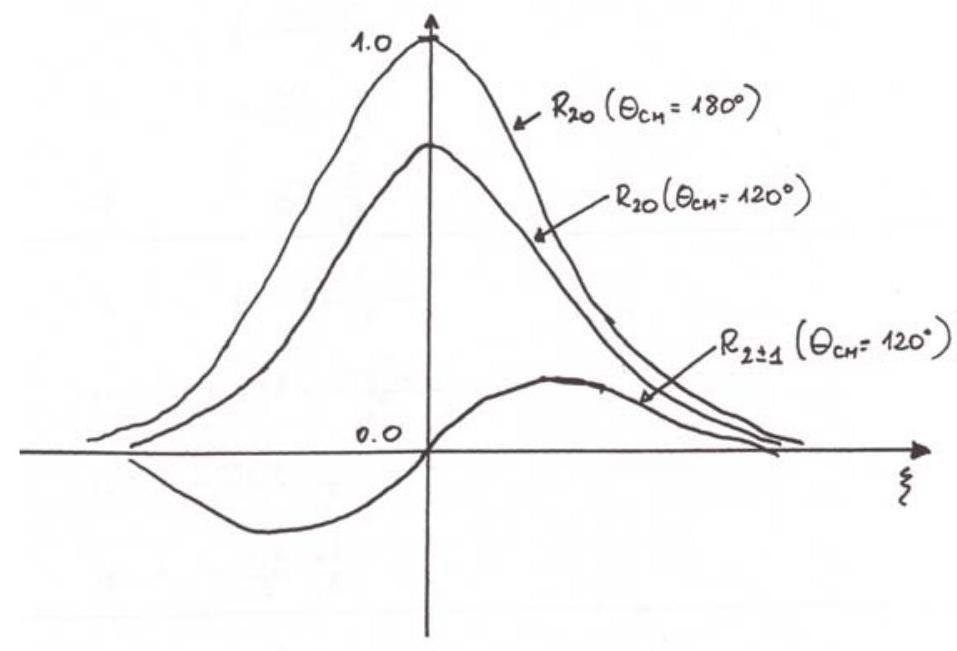
\includegraphics[max width=\textwidth]{2025_02_07_204a351db2d7f48b61ebg-039}
\end{center}

Figure 3.2: The orbital integrals $R_{20}$ and $R_{2 \pm 1}$\\
where the index " 0 " denotes the ground state. Note that equation 3.40 (and more generally 3.20 ) is valid for a fixed polarization of a ground state, thus for non-zero ground state spin one must average the excitation amplitudes over all possible magnetic substates of the ground state. This explicitly means:


\begin{equation*}
a_{k}=\frac{1}{\left(2 I_{o}+1\right)^{1 / 2}} \sum_{m_{o}} a_{k}\left(m_{o}\right) \tag{3.42}
\end{equation*}


and


\begin{equation*}
P_{k}=a_{k} a_{k}^{*} \tag{3.43}
\end{equation*}


where $a_{k}\left(m_{0}\right)$ denotes the excitation probability of state $k$ with ground state polarization $m_{o}$.\\
The formula 3.40 has been used extensively to determine reduced transition strengths:


\begin{equation*}
B\left(\lambda, I_{k} \rightarrow I_{f}\right)=\frac{1}{2 I_{k}+1}<I\|M(\lambda)\| I_{f}>^{2} \tag{3.44}
\end{equation*}


for all cases in which the one-step excitation assumption can apply. In addition to their direct applicability to weak Coulomb excitation processes, the orbital integrals $R$ give some general idea about the relationships between different modes of excitation. As an example, Fig. 3.2 shows the quadrupole orbital integrals $R_{20}$ and $R_{2 \pm 1}$ as functions of $\xi$ for $\theta_{c m}=180^{\circ}$ and $\theta_{c m}=120^{\circ}$. Note that $R_{20}$ is a maximum and $R_{2 \pm 1}$ vanishes when $\theta_{c m}=180^{\circ}$ while $\theta_{c m}=120^{\circ}$ is the optimum scattering angle for $\Delta m= \pm 1$ excitation.

The applicability of first and second order perturbation theories is limited to light-ion induced Coulomb excitation, or for heavy-ion beams, at beam energies far below the safe bombarding energy. In the case of a typical multiple Coulomb excitation experiment, the system of differential equations 3.18 must be solved numerically. It is, for example, estimated that the excitation probability of the first excited $2^{+}$state of ${ }^{248} \mathrm{Cm}$ bombarded with a $641 \mathrm{MeV}{ }^{136} \mathrm{Xe}$ beam is still sensitive to the excitation modes involving $30^{\text {th }}$-order products of the reduced matrix elements. This illustrates that the perturbation-type simplifications are generally not feasible. An efficient fast approximation to the Coulomb excitation problem is presented in Chapter 6.2.

Table 3.1a\\
Electric Collision Functions $Q_{\lambda \mu}^{E}(\epsilon, \omega)$\\
$a=\cosh \omega+\epsilon \quad b=\epsilon \cosh \omega+1 \quad c=\sqrt{\left(\epsilon^{2}-1\right)} \sinh \omega$

\begin{center}
\begin{tabular}{|c|c|c|}
\hline
$\lambda$ & $\mu$ & $Q_{\lambda \mu}^{E}(\epsilon, \omega)$ \\
\hline
1 & 0 & $\frac{1}{2} \cdot \frac{a}{b^{2}}$ \\
\hline
1 & $\pm 1$ & $-i \cdot \frac{1}{2 \sqrt{2}} \frac{c}{b^{2}}$ \\
\hline
2 & 0 & $\frac{3}{4} \cdot \frac{2 a^{2}-c^{2}}{b^{4}}$ \\
\hline
2 & $\pm 1$ & \( -i \cdot \frac{3 \sqrt{3}}{2 \sqrt{2}} \cdot \frac{a c}{b^{4}} \) \\
\hline
2 & $\pm 2$ & \( -\frac{3 \sqrt{3}}{4 \sqrt{2}} \cdot \frac{c^{2}}{b^{4}} \) \\
\hline
3 & 0 & \( \frac{15}{8} \cdot \frac{a\left(2 a^{2}-3 c^{2}\right)}{b^{6}} \) \\
\hline
3 & $\pm 1$ & \( -i \cdot \frac{15 \sqrt{3}}{16} \cdot \frac{c\left(4 a^{2}-c^{2}\right)}{b^{6}} \) \\
\hline
3 & $\pm 2$ & \( -\frac{15 \sqrt{15}}{8 \sqrt{2}} \cdot \frac{a c^{2}}{b^{6}} \) \\
\hline
3 & $\pm 3$ & $i \frac{15 \sqrt{5}}{16} \cdot \frac{c^{3}}{b^{6}}$ \\
\hline
4 & 0 & \( \frac{35}{32} \cdot \frac{8 a^{4}-24 a^{2} c^{2}+3 c^{4}}{b^{8}} \) \\
\hline
4 & $\pm 1$ & \( -i \cdot \frac{35 \sqrt{5}}{16} \cdot \frac{a c\left(4 a^{2}-3 c^{2}\right)}{b^{8}} \) \\
\hline
4 & $\pm 2$ & \( -\frac{35 \sqrt{5}}{16 \sqrt{2}} \cdot \frac{c^{2}\left(6 a^{2}-c^{2}\right)}{b^{8}} \) \\
\hline
4 & $\pm 3$ & \( i \cdot \frac{35 \sqrt{35}}{16} \cdot \frac{a c^{3}}{b^{8}} \) \\
\hline
4 & $\pm 4$ & \( \frac{35 \sqrt{35}}{32 \sqrt{2}} \cdot \frac{c^{4}}{b^{8}} \) \\
\hline
5 & 0 & \( \frac{315}{256} \cdot \frac{a\left[-14 a^{2}\left(a^{2}+9 c^{2}\right)+30 a^{4}\right]}{b^{10}} \) \\
\hline
5 & $\pm 1$ & \( -i \cdot \frac{63 \sqrt{30}}{256} \cdot \frac{c^{2} a\left(-21 c^{2}+8 a^{2}\right)}{b^{10}} \) \\
\hline
5 & $\pm 2$ & \( -\frac{315 \sqrt{210}}{128} \cdot \frac{c^{2} a\left(-3 c^{2}+2 a^{2}\right)}{b^{10}} \) \\
\hline
5 & $\pm 3$ & \( i \cdot \frac{315 \sqrt{35}}{256} \cdot \frac{c^{3}\left(9 a^{2}-b^{2}\right)}{b^{10}} \) \\
\hline
5 & $\pm 4$ & \( \frac{945 \sqrt{70}}{256} \cdot \frac{c^{4} a}{b^{10}} \) \\
\hline
5 & $\pm 5$ & \( -i \cdot \frac{945 \sqrt{7}}{256} \cdot \frac{c^{5}}{b^{10}} \) \\
\hline
6 & 0 & \( \frac{693}{256} \cdot \frac{21 a^{2}\left[-a^{2}\left(11 c^{2}+4 b^{2}\right)+5 b^{4}\right]-5 b^{6}}{b^{12}} \) \\
\hline
6 & $\pm 1$ & \( -i \cdot \frac{693 \sqrt{42}}{256} \cdot \frac{a c\left[3 a^{2}\left(-11 c^{2}+b^{2}\right)+5 b^{4}\right]}{b^{12}} \) \\
\hline
6 & $\pm 2$ & \( -\frac{693 \sqrt{105}}{512} \cdot \frac{c^{2}\left[3 a^{2}\left(-11 c^{2}+5 b^{2}\right)+b^{4}\right]}{b^{12}} \) \\
\hline
6 & $\pm 3$ & \( -i \cdot \frac{693 \sqrt{105}}{256} \cdot \frac{a c^{3}\left(-11 c^{2}+8 b^{2}\right)}{b^{12}} \) \\
\hline
6 & $\pm 4$ & \( \frac{2079 \sqrt{14}}{512} \cdot \frac{c^{4}\left(11 a^{2}-b^{2}\right)}{b^{12}} \) \\
\hline
6 & $\pm 5$ & \( -i \cdot \frac{2079 \sqrt{77}}{256} \cdot \frac{a c^{5}}{b^{12}} \) \\
\hline
6 & $\pm 6$ & \( -\frac{693 \sqrt{231}}{512} \cdot \frac{c^{6}}{b^{6}} \) \\
\hline
\end{tabular}
\end{center}

Table 3.1b\\
Magnetic Collision Functions $Q_{\lambda \mu}^{M}(\epsilon, \omega)$

\begin{center}
\begin{tabular}{|l|l|l|}
\hline
$\lambda$ & $\mu$ & $Q_{\lambda \mu}^{M}(\epsilon, \omega)$ \\
\hline
1 & 0 & 0 \\
\hline
1 & $\pm 1$ & $\mp \frac{\sqrt{2}}{4} \frac{\sqrt{\left(\epsilon^{2}-1\right)}}{b^{2}}$ \\
\hline
2 & 0 & 0 \\
\hline
2 & $\pm 1$ & $\mp \frac{3 \sqrt{6}}{16} \cdot \sqrt{\left(\epsilon^{2}-1\right)} \cdot \frac{a}{b^{4}}$ \\
\hline
2 & $\pm 2$ & $-i \frac{3 \sqrt{6}}{16} \cdot \sqrt{\left(\epsilon^{2}-1\right)} \cdot \frac{c}{b^{4}}$ \\
\hline
\end{tabular}
\end{center}

\section*{Chapter 4}
\section*{Gamma-ray Decay Following Electromagnetic Excitation }


\subsection*{4.1 Statistical tensors}
The excited state wavefunctions can be defined in a configuration space representation by the density matrix. However, it is more convenient to express the wavefunctions in the form of the statistical tensor $\rho_{k \chi}(I, I)$ which uses an angular momentum representation. The statistical tensor is an irreducible spherical tensor that expresses the state of polarization of the decaying level and is defined in terms of the density matrix by[FER65]:

\[
\rho_{k \chi}(I, I)=(2 I+1)^{1 / 2} \sum_{M M^{\prime}}(-1)^{I-M^{\prime}}\left(\begin{array}{ccc}
I & k & I  \tag{4.1}\\
-M^{\prime} & \chi & M
\end{array}\right)\langle I M| \rho\left|I M^{\prime}\right\rangle
\]

where the excitation amplitude of a substate $\mid I M>$ is explicitly denoted with two-dimensional indexing. An unpolarized excited state has a density matrix $\rho_{i}$ given by


\begin{equation*}
\langle I M| \rho\left|I M^{\prime}\right\rangle=\frac{1}{2 I_{0}+1} \sum_{M_{0}} a_{I M^{\prime}}^{*} a_{I M} \tag{4.2}
\end{equation*}


Averaging 4.1 over all possible polarizations of the unpolarized ground state gives:

\[
\rho_{k \chi}(I)=\frac{(2 I+1)^{\frac{1}{2}}}{2 I_{o}+1} \sum_{M_{o} M M^{\prime}}(-1)^{I-M^{\prime}}\left(\begin{array}{ccc}
I & k & I  \tag{4.3}\\
-M^{\prime} & \chi & M
\end{array}\right) a_{I M^{\prime}}^{*}\left(M_{o}\right) a_{I M}\left(M_{o}\right)
\]

where:


\begin{equation*}
P_{I} \equiv \rho_{00}(I) \tag{4.4}
\end{equation*}


As mentioned in section 2.1.2, the Coulomb excitation reaction can be calculated independent of the subsequent $\gamma$-ray deexcitation since the $\gamma$-ray decay processes are about $10^{8}$ times slower than the Coulomb excitation reaction. However, the statistical tensors must take into account cascade feeding from decay of higher-lying states as described in section 4.3.

\section*{$4.2 \quad \gamma$-ray angular correlations}
Formally the $\gamma$-ray angular correlation can be expressed in terms of the trace of the product of the density matrix $\rho$ and detection efficiency matrix $\epsilon$, that is, $W=\operatorname{Tr}[\rho \epsilon]$. The trace of a matrix is unaffected\\
by a unitary transformation such as a rotation, or a change of representation. An angular momentum representation is the natural form for describing the density matrix $\rho$ for the Coulomb excitation process, whereas a coordinate representation is a natural form for describing the efficiency matrix $\epsilon$. In an angular momentum representation the density matrix of coordinate space is expressed as an irreducible spherical tensor, that is, the statistical tensor $\rho_{k \chi}(I, I)$ defined above. The detection efficiency matrix also can be expressed in terms of an irreducible spherical tensor which is called the efficiency tensor $\epsilon_{k \chi}\left(I I^{\prime}\right)$ described in section 4.6. In the spherical tensor form the angular correlation transforms to the product of the statistical tensor and efficiency tensor


\begin{equation*}
W=\operatorname{Tr}[\rho \epsilon]=\sum_{L L^{\prime} k \chi} \rho_{k \chi}\left(I I^{\prime}\right) \epsilon_{k \chi}^{*}\left(I I^{\prime}\right) \tag{4.5}
\end{equation*}


Assuming a $\delta$-function point detector that has $100 \%$ detection efficiency, for any coordinate frame with the origin at the decaying nucleus, the angular distribution of the detected $\gamma$-ray radiation can be derived by transforming from the coordinate frame used for defining the efficiency tensors to that used for the statistical tensor. This gives[ALD66]:


\begin{equation*}
\frac{d^{2} \sigma}{d \Omega_{p} d \Omega_{\gamma}}=\sigma_{R}\left(\theta_{p}\right) \frac{1}{2 \gamma\left(I_{1}\right) \sqrt{\pi}} \sum_{\substack{k \text { even } \\ \chi}} \rho_{k \chi}^{*}\left(I_{1}\right) \sum_{\lambda \lambda^{\prime}} \delta_{\lambda} \delta_{\lambda^{\prime}}^{*} F_{k}\left(\lambda \lambda^{\prime} I_{2} I_{1}\right) Y_{k \chi}\left(\theta_{\gamma}, \phi_{\gamma}\right) \tag{4.6}
\end{equation*}


Here $\sigma_{R}\left(\theta_{p}\right)$ denotes the scattering-angle dependent Rutherford cross-section formula given in SI units by


\begin{equation*}
\sigma_{R}\left(\theta_{p}\right) \equiv\left(\frac{d \sigma}{d \Omega}\right)_{R}=\left(\frac{e^{2}}{16 \pi \epsilon_{0}} \frac{Z_{p} Z_{t}}{E_{c m}}\right)^{2} \frac{1}{\sin ^{4}\left(\frac{\theta_{c m}}{2}\right)} \tag{4.7}
\end{equation*}


$F_{k}\left(\lambda \lambda^{\prime}, I_{2} I_{1}\right)$ are the $\gamma-\gamma$ correlation coefficients (as defined, e.g., in [FRA65]), $Y_{k \chi}\left(\theta_{\gamma}, \phi_{\gamma}\right)$ are normalized spherical harmonics. The quantities $\delta_{\lambda}$ are the $I_{1} \rightarrow I_{2}$ transition amplitudes for multipolarity $\lambda$, related to the emission probability $\gamma\left(I_{1}\right)$ by:


\begin{equation*}
\gamma\left(I_{1}\right)=\sum_{\lambda n}\left|\delta_{\lambda}\left(I_{1} \rightarrow I_{n}\right)\right|^{2} \tag{4.8}
\end{equation*}


An explicit form of $F_{k}\left(\lambda \lambda^{\prime}, I_{2} I_{1}\right)$ can be expressed in terms of Wigner's $3-j$ and $6-j$ symbols

\[
F_{k}\left(\lambda \lambda^{\prime}, I_{2} I_{1}\right)=(-1)^{I_{1}+I_{2}-1}\left[(2 k+1)\left(2 I_{1}+1\right)(2 \lambda+1)\left(2 \lambda^{\prime}+1\right)\right]^{1 / 2}\left(\begin{array}{ccc}
\lambda & \lambda^{\prime} & k  \tag{4.9}\\
1 & -1 & 0
\end{array}\right)\left\{\begin{array}{ccc}
\lambda & \lambda^{\prime} & k \\
I_{1} & I_{1} & I_{2}
\end{array}\right\}
\]

while the transition amplitude $\delta_{\lambda}(1 \rightarrow 2)$ is given by:


\begin{equation*}
\delta_{\lambda}(1 \rightarrow 2)=i^{n(\lambda)} \frac{1}{(2 \lambda+1)!!\hbar^{\lambda+1}}\left(\frac{8 \pi(\lambda+1)}{\lambda}\right)^{1 / 2}\left(\frac{E_{\gamma}}{c}\right)^{\lambda+1 / 2} \frac{<I_{2}\|E(M) \lambda\| I_{1}>}{\left(2 I_{1}+1\right)^{1 / 2}} \tag{4.10}
\end{equation*}


where

$$
n(\lambda)= \begin{cases}\lambda & \text { for } \mathrm{E} \lambda \text { transition } \\ \lambda+1 & \text { for } \mathrm{M} \lambda \text { transition }\end{cases}
$$

Note that the transition amplitude for an electric monopole transition, $\delta_{0}$, is defined by equation 4.40.\\
The coordinate system used for evaluation of excitation probabilities is no longer convenient to determine angular distributions of gamma radiation, as it is not fixed with respect to the laboratory frame. Therefore, it is useful to redefine the $z$-axis along the beam direction with the $x$-axis in the plane of orbit in such a way that the $x$-component of the impact parameter is positive. The $y$-axis is then defined to form a right-handed system (Fig. 4.1) that is called coordinate system $C$ by Alder and Winther [ALD75].

The statistical tensors $\rho_{k \chi}$ in coordinate frame $C$ are obtained by rotation with Euler angles $\left(\frac{\pi}{2}, \frac{(\pi+\theta)}{2}, \pi\right)$ :


\begin{equation*}
\rho_{k \chi} \rightarrow \sum_{\chi^{\prime}} \rho_{k \chi^{\prime}} D_{\chi^{\prime} \chi}^{k}\left(\frac{\pi}{2}, \frac{\pi+\theta}{2}, \pi\right) \tag{4.11}
\end{equation*}


\begin{center}
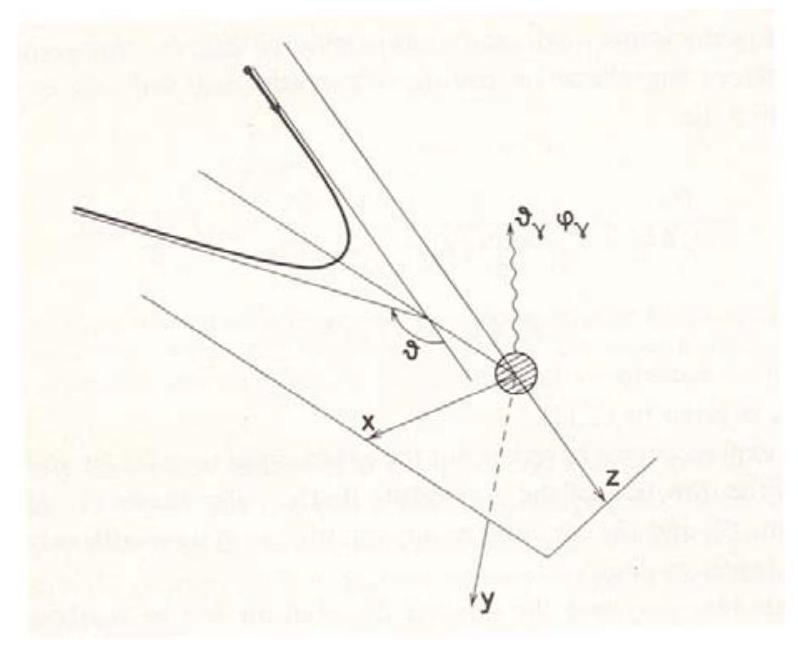
\includegraphics[max width=\textwidth]{2025_02_07_204a351db2d7f48b61ebg-043}
\end{center}

Figure 4.1: The coordinate system used to describe the $\gamma$-decay of a Coulomb-excited nucleus. The $z$-axis is chosen along the incoming beam direction, the $x$-axis is in the plane of the orbit such that the $x$-component of the velocity is positive. A $\gamma$-decay in the direction $\theta_{\gamma}, \varphi_{\gamma}$ is indicated. Note that Alder and Winther [ALD75] call this coordinate system C.\\
the rotation functions ${ }^{1} D_{\chi \chi^{\prime}}^{k}(\alpha, \beta, \gamma)$ being defined according to [BOH69]:


\begin{equation*}
D_{\chi \chi^{\prime}}^{k}(\alpha, \beta, \gamma)=e^{i \chi \alpha} d_{\chi \chi^{\prime}}^{k}(\beta) e^{i \chi^{\prime} \gamma} \tag{4.12}
\end{equation*}


with


\begin{align*}
d_{\chi \chi^{\prime}}^{k}(\beta)= & {\left[\frac{\left(k+\chi^{\prime}\right)!\left(k-\chi^{\prime}\right)!}{(k+\chi)!(k-\chi)!}\right]^{1 / 2} \cdot }  \tag{4.13}\\
& \sum_{m}\binom{k+\chi}{k-\chi^{\prime}-m}\binom{k-\chi}{m}(-1)^{k-\chi^{\prime}-m}\left[\cos \frac{\beta}{2}\right]^{2 m+\chi+\chi^{\prime}}\left[\sin \frac{\beta}{2}\right]^{2 k-2 m-\chi-\chi^{\prime}}
\end{align*}


where $\left(\frac{n}{m}\right)$ is the binomial coefficient. Inserting 4.10 and 4.11 into 4.9 gives:


\begin{equation*}
\rho_{k \chi} \rightarrow(-1)^{\chi} \cdot \sum_{\chi^{\prime}} i^{\chi^{\prime}} d_{\chi^{\prime} \chi}^{k}\left(\frac{\pi+\theta}{2}\right) \rho_{k \chi^{\prime}} \tag{4.14}
\end{equation*}


A complete description of the $\gamma$-decay also must involve correction for the depolarization of the excited levels due to the hyperfine interaction, i.e., the interaction between the stripped electron shells of the surrounding atom and the nucleus. This effect can be taken into account by introducing the $k$-dependent time-integral attenuation coefficients, $G_{k}$, that multiply the statistical tensors (the attenuation coeficients, $G_{k}$, are described in Section 4.4). The attenuation of the angular distribution due to the hyperfine interactions is usually significant in the case of thin-target experiments, while all the $G_{k}$ 's equal unity if the decaying nucleus has been stopped in the target prior to the $\gamma$ decay. The basic angular correlation equation 4.6 can be expressed in terms of the angular distribution tensors, $R_{k \chi}$, which include the hyperfine interaction effects:


\begin{equation*}
\frac{d^{2} \sigma}{d \Omega_{p} d \Omega_{\gamma}}=\sigma_{R}\left(\theta_{p}\right) \sum_{k \chi} R_{k \chi}\left(I, I_{f}\right) Y_{k \chi}\left(\theta_{\gamma}, \phi_{\gamma}\right) \tag{4.15}
\end{equation*}


\footnotetext{${ }^{1}$ Although the reference coordinate frame and the $\gamma$-ray detector-fixed coordinate frames are unambiguously defined, there are several possible intermediate frames that can be used to define the Euler angles. Bohr and Mottelson [BOH69] use the $z-y-z$ sequence of rotations adopted in nuclear and particle physics. Appendix A of "Classical Mechanics" by Goldstein, Poole, \& Safko, discusses the $z-x-z$ sequence of rotations adopted in classical mechanics, the $z-y-z$ sequence adopted in nuclear and particle physics, and the $x-y-z$ sequence of rotations adopted by the US and UK aerodynamicists. Care must be taken to adopt one common sequence of rotations.
}
where:\\
\$\$

\begin{equation*}
R_{k \chi}\left(I, I_{f}\right) \equiv \frac{1}{2 \gamma(I) \sqrt{\pi}} G_{k} \rho_{k \chi} \sum_{\lambda \lambda^{\prime}} \delta_{\lambda} \delta_{\lambda^{\prime}}^{*} F_{k}\left(\lambda \lambda^{\prime}, I_{f} I\right) \tag{4.16}
\end{equation*}

\$\$\\
is the angular distribution tensor describing the mixed electric and magnetic transition from a state $I$ to a state $I_{f}$. The Coulomb excitation statistical tensors are purely real for even values of $k$ in the frame of coordinates introduced above, thus $\rho_{k \chi}=\rho_{k \chi}^{*}$. Moreover, taking into account the selection rules for electromagnetic transitions, the products $\delta_{\lambda} \delta_{\lambda^{\prime}}^{*}$ also are real and thus the angular distribution tensors are purely real.

\subsection*{4.3 Cascade deexcitation feeding}
The above formulas describe $\gamma$-decay of a level fed directly, and exclusively, by the Coulomb excitation reaction prior to decay feeding. For multiple Coulomb excitation, significant feeding from the deexcitation cascade decay of higher-lying levels must be taken into account. The related modification of the angular distribution tensors can be expressed as:


\begin{equation*}
R_{k \chi}\left(I, I_{f}\right) \longrightarrow R_{k \chi}\left(I, I_{f}\right)+\sum_{n} R_{k \chi}\left(I_{n}, I\right) H_{k}\left(I, I_{n}\right) \tag{4.17}
\end{equation*}


where the summation extends over all levels $I_{n}$ directly feeding level $I$. The explicit formula for the $H_{k}$ coefficients is:

\[
H_{k}\left(I, I_{n}\right)=\frac{\left[(2 I+1)\left(2 I_{n}+1\right)\right]^{1 / 2}}{\gamma(I)} \sum_{\lambda}(-1)^{I+I_{n}+\lambda+k}\left|\delta_{\lambda}\right|^{2}(1+c(\lambda))\left\{\begin{array}{ccc}
I & I & k  \tag{4.18}\\
I_{n} & I_{n} & \lambda
\end{array}\right\}
\]

where $c(\lambda)$ is the internal conversion coefficient for the $I_{n} \rightarrow I$ transition. Note that for an electric monopole transition $c(0)=0$. Formula 4.17 is used to sequentially modify the deexcitation statistical tensors, starting from the highest levels having non-negligible population. This operation transforms the deexcitation statistical tensors, which are inserted into 4.15 to give the unperturbed angular distributions following Coulomb excitation.

In addition, it is necessary to take into account several experiment-related perturbations, namely the deorientation effect, relativistic corrections due to in-flight decay, internal conversion, and the geometry of the $\gamma$-ray detectors. These effects can be significant when using thin targets and heavy ion beams. An overview of the methods employed by GOSIA to account for these experimental perturbations is presented in sections $4.4-4.7$

\subsection*{4.4 Nuclear deorientation for recoil in vacuum}
In typical Coulomb excitation experiments, both the scattered projectile and target nuclei recoil into vacuum in highly-excited, highly-ionized, atomic states which subsequently decay to a ground state. The strong fluctuating hyperfine fields of the deexciting atom depolarize the nuclear state alignment; this effect is known as the nuclear deorientation effect. This attenuates the angular distribution of the de-excitation $\gamma$ rays which can be taken into account by introducing the spin and lifetime dependent attenuation coefficients $G_{k}$ that multiply the decay statistical tensors.

The magnetic interaction between the magnetic dipole moments of the excited nuclear states and the $\sim 10^{4} T$ atomic hyperfine magnetic fields produce the dominant hyperfine interaction responsible for the deorientation. If this atomic hyperfine magnetic field could be predicted accurately then the deorientation effect would provide a powerful probe for measuring the magnitude of the magnetic dipole moments of excited nuclear states. When the nucleus recoils out of the target the highly-ionized and highly-excited atomic structure decays rapidly by a cascade of photons, as well as Auger electrons, with time constants as short as a picosecond. This rapid atomic decay produces rapidly fluctuating hyperfine atomic fields. Eventually the atomic structure deexcites to the equilibrium atomic ground-state configuration which depends on the charge state of the ion. The deorientation effect has a complicated dependence on thedynamic equilibrium of the charge state, the lifetimes of the excited states, the atomic and nuclear spins, and dephasing effects.

Since these complicated and stochastic atomic processes cannot be predicted accurately at the present time, it is necessary to resort to simple models with parameters fitted to available deorientation effect data.

The initial fluctuating stage during which the excited atomic structure rapidly deexcites can be modelled by the Abragam and Pound theory [ABR53]. This theory works well in situations when the ions recoil into high-pressure gas since the atomic structure of the recoiling ions is reexcited by each collision with a gas molecule. However, significant discrepancies from the Abragam and Pound model occur for recoil into vacuum due to the important contribution of the static interaction. Theories of the static hyperfine interaction of the atomic structure of the ground state atomic configuration are available [GOL78].

Currently GOSIA uses a modified version of the Two-State Model of the deorientation effect ( [BOS77], [BRE77]), which seems to correlate well with existing data despite the far-reaching simplification enforced by the complexity of the problem[KAV90]. Within the framework of the Two-State Model, the hyperfine field may either belong to a "fluctuating" state, during which the excited electronic structure of the atom decays to the atomic ground state, or to a "static" state, corresponding to an equilibrium atomic groundstate configuration. The excitation and decay of stripped electron shells is a complicated stochastic process making it difficult to describe exactly, therefore it is assumed that all atomic processes taking place in the fluctuating state are purely random. The rate of transition from the fluctuating to static state, $\Lambda^{*}$, is an adjustable parameter of the model that is not fit by Gosia. The time-dependent deorientation coefficients $G_{k}(t)$ then are given by:


\begin{equation*}
G_{k}(t)=e^{-\Lambda^{*} t} G_{k}^{(f l u c t .)}(t)+\int_{o}^{t} \Lambda^{*} G_{k}^{(\text {fluct. })}\left(t^{\prime}\right) \cdot e^{-\Lambda^{*} t^{\prime}} G_{k}^{(\text {stat. })}\left(t-t^{\prime}\right) d t^{\prime} \tag{4.19}
\end{equation*}


The references [BOS77], [BRE77], plus references therein, provide the details of the derivation.\\
The static-state attenuation factor $G_{k}^{(s t a t)}$ is expressed as

\[
G_{k}^{(s t a t)}(t)=\sum_{i} p\left(J_{i}\right) \cdot \sum_{F_{i} F_{i}^{\prime}} \frac{\left(2 F_{i}+1\right)\left(2 F_{i}^{\prime}+1\right)}{2 J_{i}+1}\left\{\begin{array}{ccc}
F_{i} & F_{i}^{\prime} & k  \tag{4.20}\\
I & I & J_{i}
\end{array}\right\}^{2} \cos \omega_{F F^{\prime}} t
\]

where $F_{i}$ is the vector sum of the nuclear spin $I$ and the electronic spin $J_{i}$ of the ground state of the deexcited atom, i.e. the ground state spin of an atom with the charge number equal to the charge number of the investigated nucleus minus the number of stripped electrons. The angular frequency $\omega_{F F^{\prime}}$ is given by

$$
\omega_{F F^{\prime}}=\frac{a\left(J_{i}\right)}{2 \hbar}\left[F(F+1)-F^{\prime}\left(F^{\prime}+1\right)\right]
$$

Note that when $F=F^{\prime}$, then $\cos \omega_{F F} t=1$.\\
Practically, averaging over the fluctuating state atomic spins $J_{i}$ in 4.20 is not possible since the spin distribution is not known. Therefore one must use a single mean value of $J_{i}$, treated as one more model parameter. The parameter $a\left(J_{i}\right)$ is defined as:


\begin{equation*}
a\left(J_{i}\right)=\mu_{n} g \frac{\bar{H}}{J_{i}} \tag{4.21}
\end{equation*}


where $\mu_{n}$ is the nuclear magneton and $g$ stands for the gyromagnetic factor. The mean magnetic field $\bar{H}$ in the fluctuating state is approximated as:


\begin{equation*}
\bar{H}=K Z\left(\frac{v}{c}\right)^{x} \tag{4.22}
\end{equation*}


with both $K$ and $x$ being adjustable parameters best fit to data systematics[GOL77].\\
Define $\left\langle\alpha_{k}\right\rangle$ to be:

\[
\left\langle\alpha_{k}\right\rangle \equiv \sum_{i} p\left(J_{i}\right) \cdot \sum_{F_{i}} \frac{\left(2 F_{i}+1\right)^{2}}{2 J_{i}+1}\left\{\begin{array}{ccc}
F_{i} & F_{i} & k  \tag{4.23}\\
I & I & J_{i}
\end{array}\right\}^{2}
\]

Since

$$
\sum_{F_{i} F_{i}^{\prime}} \frac{\left(2 F_{i}+1\right)\left(2 F_{i}^{\prime}+1\right)}{2 J_{i}+1}\left\{\begin{array}{ccc}
F_{i} & F_{i}^{\prime} & k \\
I & I & J_{i}
\end{array}\right\}^{2}=1
$$

then $G_{k}^{(s t a t)}(t)$ can be written in the form


\begin{equation*}
G_{k}^{(s t a t)}(t)=\left\langle\alpha_{k}\right\rangle+\left(1-\left\langle\alpha_{k}\right\rangle\right) e^{-\Gamma t} \tag{4.24}
\end{equation*}


In equation 4.24 , the parameter $\Gamma$ is the width of the Larmor frequency distribution resulting from the assumption of many ionic ground states, as well as many long-lived excited atomic states, that are involved in the static part of the interaction. This distribution is assumed to be Lorentzian, with $\Gamma$ treated as an adjustable parameter of the model not fitted by Gosia.

The standard Nikolayev-Dmitriev stripping formula [NIK68] is used to determine the atomic charge states and the corresponding atomic ground state spins $J_{i}$. The term $p\left(J_{i}\right)$ in [4.23] is the discrete distribution of electronic angular momenta $J_{i}$ which is evaluated by defining a parameter $h$ :


\begin{equation*}
h=\frac{1}{1+\left(\frac{0.012008 c}{v} Z^{0.45}\right)^{5 / 3}} \tag{4.25}
\end{equation*}


which includes the best-fit constants given by [NIK68]. Then the Gaussian charge state distribution is taken to be centered around $Q_{o}$ with a Gaussian width $\sigma_{Q}$ given by


\begin{align*}
Q_{o} & =Z \cdot(h)^{0.6}  \tag{4.26}\\
\sigma_{Q} & =\left(Q_{o}(1-h)\right)^{1 / 2}
\end{align*}


The fluctuating-state attenuation factor $G^{(f l u c t .)}(t)$ is given by:


\begin{equation*}
G^{\text {fluct }}(t)=\left(1-\lambda_{k} \tau_{c}\right) \exp \left(-\lambda_{k} t\right) \tag{4.27}
\end{equation*}


where the correlation time $\tau_{c}$ is the mean time between random reorientations of the fluctuating hyperfine field and:


\begin{equation*}
\lambda_{k}=\frac{1-\left\langle\alpha_{k}\right\rangle}{\tau_{c}}\left(1-\exp \left(\frac{-\left\langle\omega^{2}\right\rangle \tau_{c}^{2}}{1-\left\langle\alpha_{k}\right\rangle}\right)\right) \tag{4.28}
\end{equation*}


with $\left\langle\omega^{2}\right\rangle$ being the average Larmor frequency in the fluctuating state field:


\begin{equation*}
\left\langle\omega^{2}\right\rangle=\frac{1}{3} k(k+1) \sum_{J_{i}} p\left(J_{i}\right) \frac{a^{2}\left(J_{i}\right)}{\hbar^{2}} J_{i}\left(J_{i}+1\right) \tag{4.29}
\end{equation*}


Formula 4.27 is valid only for $t$ much larger than $\tau_{c}$. Taking into account that $\tau_{c}$ is of the order of a few picoseconds, which is the order of a typical lifetime of the collective nuclear levels, and that the time-integral attenuation coefficients are required, we have to introduce a correction to 4.27 in the time range of $\tau_{c}$. Since $G^{(f l u c t .)}(t)$ also can be derived for $t \rightarrow 0$, it is practical to introduce an interpolating function between time ranges $t \rightarrow 0$ and $t$ much greater than the correlation time $\tau_{c}$, being chosen as a linear combination of two exponential time-decay functions in order to keep the mathematics at a minimum. This procedure yields for the time-integral coefficients $G_{k}$ :


\begin{equation*}
G_{k}=\lambda_{I} \int_{o}^{\infty} G_{k}(t) \exp \left(-\lambda_{I} t\right) d t=G_{k}^{B S}\left[1+\frac{\lambda_{k} \tau_{I}\left(r-2 p^{2} \tau_{I} \tau_{c}\right)}{\left(r+p \tau_{I}\right)\left(r+2 p \tau_{I}\right)}\right] \tag{4.30}
\end{equation*}


where:


\begin{equation*}
G^{B S}=\frac{1}{r}\left[1+\Lambda^{*} \tau_{I}\left(\frac{1+<\alpha_{k}>\Gamma \tau_{I}}{1+\Gamma \tau_{I}}\right)\right] \tag{4.31}
\end{equation*}


is an original formula from $[\operatorname{BOS} 77], \tau_{I}=1 / \lambda_{I}$ is the mean lifetime of a nuclear state of spin $I$, while $r$ and $p$ are given by:


\begin{gather*}
r=\left(\Lambda^{*}+\lambda_{k}\right) \tau_{I}+1  \tag{4.32}\\
p=\frac{\left(9 \lambda_{k}^{2}+8 \lambda_{k} \tau_{c}\left(\left\langle\omega^{2}\right\rangle-\lambda_{k}^{2}\right)\right)^{1 / 2}-3 \lambda_{k}}{4 \lambda_{k} \tau_{c}} \tag{4.33}
\end{gather*}


The correction to the original model in most cases does not exceed $10 \%$ and is easily evaluated since no additional parameters have been introduced.

For multiple Coulomb excitation the angular distribution tensors for any state must include the contributions for feeding from higher excited states as given in equation 4.17-4.18. Thus, in addition to deorientation of transitions from a given state, the feeding transitions to this state also are deoriented as given by eq. 4.17.

The recommended default parameters of the nuclear deorientation model are listed in table 4.1 and section 7.3, in the description of the VAC switch of the CONT suboption of GOSIA. Kavka [KAV90] analysed deorientation data collected as a by-product of Coulomb excitation studies for 9 nuclei and found that using the default parameters the above two-state model reproduces the data well. As a consequence, GOSIA uses the Two-State Model to account for the deorientation effect. Currently Gosia does not fit the deorientation model parameters to the data. If an accurate model of the deorientation effect becomes available then GOSIA could be used directly to measure static magnetic moments of excited states.

Table 4.1: Default values of the Two-State Model parameters used in GOSIA

\begin{center}
\begin{tabular}{|c|c|c|}
\hline
\multicolumn{2}{|c|}{Nuclear gyromagnetic factor} & $g=\frac{Z}{A}$ \\
\hline
\multirow{4}{*}{Fluctuating component} & Hyperfine field coefficient & $K=600 T$ \\
\cline { 2 - 3 }
 & Hyperfine field exponent & $x=0.6$ \\
\cline { 2 - 3 }
 & Average atomic spin & $J=3$ \\
\cline { 2 - 3 }
 & Correlation time & $\tau_{c}=3.5 \mathrm{ps}$ \\
\hline
Static component & FWHM of frequency distribution & $\Gamma=0.02 \mathrm{ps} \mathrm{s}^{-1}$ \\
\hline
\multicolumn{2}{|c|}{Fluctuating to static transition rate} & $\Lambda^{*}=0.0345 \mathrm{ps}^{-1}$ \\
\hline
\end{tabular}
\end{center}

\subsection*{4.5 Relativistic Angular Distribution Correction}
The coordinate system used to evaluate the angular distribution of the decay $\gamma$-rays, shown in Figure 4.1, is fixed with respect to the photon-emitting nucleus with the $z$-axis pointing along the incoming beam direction and with the $y$-axis perpendicular to the scattering plane. For experimental work it is necessary to transform the $\gamma$-ray angular distribution into the laboratory frame of reference with respect to which the $\gamma$-ray detectors are fixed, while keeping the $z$-axis pointing along the incoming beam direction. For heavy-beam, thin-target experiments, the recoil velocity can reach up to $10 \%$ of the velocity of light and thus the transformation from the photon-emitting recoil-nucleus centered system of coordinates to the laboratory system must be Lorentzian. The exact relativistic transformation between the moving to laboratory frames is easy to apply numerically [HAG63], unfortunately this transformed angular distribution is not expressed as an expansion in spherical harmonics. There are considerable advantages to transform the spherical harmonic expression in the recoil nucleus frame directly into a spherical harmonic expansion in the laboratory frame. The first order description of this transform is given in [ALD75]. Gosia uses a more accurate alternate approach, based on second-order Lorentz transformation of angular distribution tensors, that was developed by Lesser and Cline [[LES71],[LES10]]. This analytic second-order relativistic transformation is accurate to $\leq 0.1 \%$ for $\beta=\frac{v_{\text {recoil }}}{c} \leq 0.1$, fits well the deexcitation formalism employed by the code, and facilitates a fast, closed-form integration over the photon detector geometry.

Using $R N$ to specify the recoiling nucleus centered system with the $z$-axis defined by the recoil direction, and $L A B$ for the laboratory-fixed system, then to second order in $\beta$ the relativistic transformation is:


\begin{equation*}
\frac{d W^{L A B}(\theta, \phi)}{d \Omega_{\gamma}}=\left\{\left(1-\beta^{2}\right)+\beta U+\frac{1}{2} \beta^{2} V\right\} \frac{d W^{R N}(\theta, \phi)}{d \Omega_{\gamma}} \tag{4.34}
\end{equation*}


where the angular distribution in the recoil nucleus system is written as:


\begin{equation*}
\frac{d W^{R N}(\theta, \phi)}{d \Omega_{\gamma}}=\sum_{k_{\chi} \text { even }} a_{k \chi} Y_{k \chi}(\theta, \phi) \tag{4.35}
\end{equation*}


which is basically a short form of equation 4.6. It is assumed that the statistical tensors $\rho_{k \chi}$ in the recoil nucleus frame, given by equation 4.6, have been modified to account for the $\gamma$-ray feeding from above as well as the deorientation effect. As shown in reference[LES10], the relativistic transformation can be ordered in powers of $\beta$ giving:


\begin{equation*}
\frac{d W^{L A B}(\theta, \phi)}{d \Omega_{\gamma}}=\sum_{k_{\chi} \text { even }} a_{k \chi} Y_{k \chi}(\theta, \phi)+\beta \sum_{\substack{k \\ o d d}} b_{k \chi} Y_{k \chi}(\theta, \phi)+\beta^{2} \sum_{\substack{k \\ \text { even }}} b_{k \chi} Y_{k \chi}(\theta, \phi) \tag{4.36}
\end{equation*}


where the $b_{k \chi}$ tensors result from equation 4.34 and are linear combinations of the $a_{k \chi}$ components as given in Table 2.2. The result of equation 4.36 can be represented as modified statistical tensors and rotated back to the laboratory frame of coordinates with $z$ along the beam direction. It should be noted that due to the relativistic correction, terms involving odd- $k$ spherical harmonics are introduced and the maximum $k$ value is increased by 2 . Table 2.2 has been evaluated for multipolarities up to $\lambda=3$, i.e. $k \leq 6$ in the recoil nucleus frame leading to $k \leq 8$ in the laboratory frame. Multipoles with $\lambda>3$ have lifetimes that are much longer than the time of flight of the recoiling nuclei and thus the recoiling nuclei are stopped before $\gamma$-ray decay.

Table 4.2\\
Relativistic transformation of the angular distribution coefficients $b_{k \chi}$

\begin{center}
\begin{tabular}{|c|c|c|c|c|c|}
\hline
\multicolumn{3}{|r|}{Odd k} & \multicolumn{3}{|r|}{Even k} \\
\hline
$k$ & $\chi$ & $b_{k \chi}$ & $k$ & $\chi$ & $b_{k \chi}$ \\
\hline
1 & 0 & $\frac{2}{\sqrt{3}} a_{00}-\frac{2}{\sqrt{15}} a_{20}$ & 2 & 0 & $\frac{2}{\sqrt{5}} a_{00}-\frac{10}{7} a_{20}+\frac{12}{7 \sqrt{5}} a_{40}$ \\
\hline
1 & 1 & $-\frac{1}{\sqrt{5}} a_{21}$ & 2 & 1 & $-\frac{17}{14} a_{21}+\frac{2 \sqrt{6}}{7} a_{41}$ \\
\hline
3 & 0 & \( \frac{12}{\sqrt{35}} a_{20}-\frac{4}{\sqrt{7}} a_{40} \) & 2 & 2 & $-\frac{4}{7} a_{22}+\frac{2 \sqrt{3}}{7} a_{42}$ \\
\hline
3 & 1 & \( \frac{8 \sqrt{2}}{\sqrt{35}} a_{21}-\sqrt{\frac{15}{7}} a_{41} \) & 4 & 0 & \( \frac{8 \sqrt{5}}{7} a_{20}-\frac{380}{77} a_{40}+\frac{100}{11 \sqrt{13}} a_{60} \) \\
\hline
3 & 2 & $\frac{4}{\sqrt{7}} a_{22}-\frac{2 \sqrt{3}}{\sqrt{7}} a_{42}$ & 4 & 1 & \( \frac{20 \sqrt{6}}{21} a_{21}-\frac{723}{154} a_{41}+\frac{20 \sqrt{70}}{11 \sqrt{39}} a_{61} \) \\
\hline
3 & 3 & $-a_{43}$ & 4 & 2 & \( \frac{20 \sqrt{3}}{21} a_{22}-\frac{306}{77} a_{42}+\frac{40 \sqrt{14}}{11 \sqrt{39}} a_{62} \) \\
\hline
5 & 0 & $\frac{10}{\sqrt{11}} a_{40}-\frac{30}{\sqrt{143}} a_{60}$ & 4 & 3 & \( -\frac{61}{22} a_{43}+\frac{40 \sqrt{3}}{11 \sqrt{13}} a_{63} \) \\
\hline
5 & 1 & $\frac{4 \sqrt{6}}{\sqrt{11}} a_{41}-\frac{5 \sqrt{35}}{\sqrt{143}} a_{61}$ & 4 & 4 & \( -\frac{12}{11} a_{44}+\frac{20 \sqrt{5}}{11 \sqrt{13}} a_{64} \) \\
\hline
5 & 2 & \( \frac{2 \sqrt{21}}{\sqrt{11}} a_{42}-\frac{20 \sqrt{2}}{\sqrt{143}} a_{62} \) & 6 & 0 & $\frac{210}{11 \sqrt{13}} a_{40}-\frac{574}{55} a_{60}$ \\
\hline
5 & 3 & $\frac{8}{\sqrt{11}} a_{43}-\frac{15 \sqrt{3}}{\sqrt{143}} a_{63}$ & 6 & 1 & \( \frac{14 \sqrt{210}}{11 \sqrt{13}} a_{41}-\frac{1121}{110} a_{61} \) \\
\hline
5 & 4 & \( \frac{6}{\sqrt{11}} a_{44}-\frac{10 \sqrt{5}}{\sqrt{143}} a_{64} \) & 6 & 2 & \( \frac{28 \sqrt{42}}{11 \sqrt{13}} a_{42}-\frac{104}{11} a_{62} \) \\
\hline
5 & 5 & $-\frac{5}{\sqrt{13}} a_{65}$ & 6 & 3 & $\frac{84 \sqrt{3}}{11 \sqrt{13}} a_{43}-\frac{181}{22} a_{63}$ \\
\hline
7 & 0 & $\frac{56}{\sqrt{195}} a_{60}$ & 6 & 4 & $\frac{42 \sqrt{5}}{11 \sqrt{13}} a_{44}-\frac{358}{55} a_{64}$ \\
\hline
7 & 1 & $\frac{32}{\sqrt{65}} a_{61}$ & 6 & 5 & $-\frac{43}{10} a_{65}$ \\
\hline
7 & 2 & $\frac{8 \sqrt{3}}{\sqrt{13}} a_{62}$ & 6 & 6 & $-\frac{8}{5} a_{66}$ \\
\hline
7 & 3 & \( \frac{16 \sqrt{2}}{\sqrt{39}} a_{63} \) & 8 & 0 & $\frac{672}{5 \sqrt{221}} a_{60}$ \\
\hline
7 & 4 & $\frac{8 \sqrt{11}}{\sqrt{65}} a_{64}$ & 8 & 1 & $\frac{144 \sqrt{21}}{5 \sqrt{221}} a_{61}$ \\
\hline
7 & 5 & $\frac{16 \sqrt{2}}{\sqrt{65}} a_{65}$ & 8 & 2 & \( \frac{36 \sqrt{12}}{\sqrt{221}} a_{62} \) \\
\hline
7 & 6 & $\frac{8}{\sqrt{15}} a_{66}$ & 8 & 3 & \( \frac{24 \sqrt{22}}{\sqrt{221}} a_{63} \) \\
\hline
7 & 7 & 0 & 8 & 4 & \( \frac{144 \sqrt{11}}{5 \sqrt{221}} a_{64} \) \\
\hline
 &  &  & 8 & 5 & \( \frac{72 \sqrt{2}}{5 \sqrt{17}} a_{65} \) \\
\hline
 &  &  & 8 & 6 & \( \frac{24 \sqrt{7}}{5 \sqrt{17}} a_{66} \) \\
\hline
 &  &  & 8 & 7 & 0 \\
\hline
 &  &  & 8 & 8 & 0 \\
\hline
\multicolumn{6}{|r|}{$b_{k,-\chi}=(-1)^{\chi} b_{k \chi}^{*}=(-1)^{\chi} b_{k \chi}$ since $b_{k \chi}$ are real.} \\
\hline
\end{tabular}
\end{center}

The relativistic correction formalism [[LES71], [LES10]], presented above, results in an elegant modification of the decay statistical tensors and is used to the full extent in GOSIA despite the minor importance of some of the correction terms involved. Note that the $b_{k \chi}$ are linear combinations of the recoil-nucleus frame angular distribution coefficients $a_{k \chi}$, that is, the coefficients of the spherical harmonic expansion in the laboratory frame are simply related to those in the recoil-nucleus frame. Thus the angular distribution coefficients in the recoil-nucleus frame can be fit directly to the data. This could be useful for making a fit\\
to determine the deorientation effect attenuation coefficients $G_{k}$ which are included in $a_{k \chi}$ as defined by equations 4.15, 4.16.

\subsection*{4.6 Gamma detection efficiency tensor}
\subsection*{4.6.1 General theory for the efficiency tensor}
Discussion of the angular distribution of the $\gamma$-rays so far has assumed that the photon is detected by a point $\gamma$-ray detector with a $100 \%$ detection-efficiency at a radius $r$ and with a $\delta$-function angular width at the location $\left(\theta_{0}, \phi_{0}\right)$. The angles $\left(\theta_{0}, \phi_{0}\right)$ are given relative to the same reference frame used for determining the statistical tensor. To reproduce an experimental angular distribution it is necessary to take into account the probability of $\gamma$-ray detection, the finite size of the $\gamma$-ray detectors, as well as $\gamma$-ray absorption in absorbers and the detector. All these effects attenuate and smooth the observed $\gamma$-ray angular correlations[FER65, ROS53].

Direct numerical integration over the finite-size and geometry of the $\gamma$-ray detectors would be time consuming to perform since it must be performed separately for each $\gamma$-ray transition energy for each $\gamma$ ray detector. This would be impractical for Coulomb excitation measurements that involve population of many levels where several hundred coincident $\gamma$-ray transitions may be detected using multi-detector arrays like Gammasphere having $\sim 100$ individual $\gamma$-ray detectors. The much more efficient, and elegant approach is to use a spherical harmonic decomposition of the detection efficiency of individual detectors similar to the approach used for the relativistic angular distribution correction. This approach, as developed by Ferguson[FER65], uses the concept of the efficiency tensor $\epsilon_{k \chi}$ which is an irreducible spherical tensor introduced in chapter 4.2. The measured angular distribution then is given by the trace of the statistical and efficiency matrices as given by equation 4.5.

Calculation of the efficiency tensor for an individual $\gamma$-ray detector is greatly facilitated if it is performed in the principal axis frame of the individual $\gamma$-ray detector. This calculated detection efficiency tensor then has to be rotated from the individual-detector principal-axis frame to the reference frame used to calculate the statistical tensors and for specifying the angles $\theta_{i} \phi_{i}$ of the individual detectors. It will be shown that this approach is simplified if the individual $\gamma$-ray detector has axial symmetry about the axis from the emitter nucleus to a reference point in the detector. The following outline closely follows the derivation given by Ferguson[FER65].

Define the coordinate frame for the ideal $\delta$-function point $\gamma$-ray detector to be the principal axis with coordinates $(r, \theta=0, \phi=0)$ and the origin being the nucleus that emits the photon. In this frame the detection efficiency tensor $\epsilon_{k \chi}^{\delta}$ for a $\delta$-function point $\gamma$-ray detector can be expressed as the product of the radiation parameter $C_{k \chi}\left(L p, L^{\prime} p^{\prime}\right)$, where $L, L^{\prime}$ specify the total angular momenta and $p, p^{\prime}$ specify the polarization, with the rotation matrix that transforms from the statistical tensor reference frame to the principal-axis frame fixed to the individual $\delta$-function point $\gamma$-ray detector. That is,


\begin{equation*}
\epsilon_{k \chi}^{\delta}\left(L p, L^{\prime} p^{\prime}\right)=\sum_{\chi^{\prime}} \mathcal{D}_{\chi \chi^{\prime}}^{k *}\left(\Re^{-1}\right) C_{k \chi^{\prime}}\left(L p, L^{\prime} p^{\prime}\right)=\sum_{\chi^{\prime}} \mathcal{D}_{\chi^{\prime} \chi}^{k}(\Re) C_{k \chi^{\prime}}\left(L p, L^{\prime} p^{\prime}\right) \tag{4.37}
\end{equation*}


where the rotation is $\Re=\left(\phi, \theta, \phi^{\prime}\right)$. The Euler angles $\phi$ and $\theta$ of this rotation are the coordinates of the $\delta$-function point detector in the statistical-tensor reference frame, and $\phi^{\prime}$ represents a reorientation of the polarization sensitivity of the detector to align with the coordinate frame used to describe the photon wave functions.

For a finite-size $\gamma$-ray detector, define a principal axis coordinate frame such that the nominal center of the detector has coordinates $(r, \theta=0, \phi=0)$ and the origin is the nucleus that emits the photon. Then the efficiency tensor for this finite detector $\epsilon_{k \chi}^{F D}$ can be expressed in terms of the $\delta$-function point detector relation for the arbitrary point $\left(r_{0}, \theta_{0}, \phi_{0}\right)$ and integrating over the finite size of the detector.


\begin{equation*}
\epsilon_{k \chi}^{F D}\left(L p, L^{\prime} p^{\prime}\right)=\sum_{\chi^{\prime}} \int \mathcal{D}_{\chi^{\prime} \chi}^{k}\left(\Re_{0}\right) C_{k \chi^{\prime}}\left(L p, L^{\prime} p^{\prime}\right) \varepsilon\left(r_{0}, \theta_{0}, \phi_{0}\right) r_{0}^{2} d r_{0} d \Omega_{0} \tag{4.38}
\end{equation*}


where $\varepsilon\left(r_{0}, \theta_{0}, \phi_{0}\right)$ is the local probability of $\gamma$-ray detection per unit volume. At the energy $\left(E_{\gamma}\right)$ the detection efficiency per unit volume separates into two factors


\begin{equation*}
\varepsilon\left(r_{0}, \theta_{0}, \phi_{0}\right)=\frac{e^{-\tau x}}{r^{2}} E\left(r_{0}, \theta_{0}, \phi_{0}\right) \tag{4.39}
\end{equation*}


where $\frac{e^{-\tau x}}{r^{2}}$ takes into account the attenuation of the $\gamma$-radiation due to absorption in the detector or other absorbers with linear absorption coefficient $\tau$, and where $E\left(r_{0}, \theta_{0}, \phi_{0}\right)$ is the total-energy detection efficiency at a point in the detector; evaluation of the latter requires use of Monte Carlo techniques to include summing of multiple $\gamma$-ray interactions in the detector.

If the $\gamma$-ray detector is not sensitive to polarization, then the efficiency tensor for a finite detector can be summed over both polarizations which leads to the factor 2 in equation 4.40


\begin{equation*}
\epsilon_{k \chi}^{F D}\left(E_{\gamma}\right)=2 C_{k 0}\left(L L^{\prime}\right) \int \varepsilon\left(E_{\gamma}, r_{0}, \theta_{0}, \phi_{0}\right) \mathcal{D}_{\chi^{\prime} \chi}^{k}\left(\phi_{0}, \theta_{0}, 0\right) d r_{0} d \Omega_{0} \tag{4.40}
\end{equation*}


where $\epsilon_{k \chi}^{F D}\left(E_{\gamma}\right)$ is a function of $E_{\gamma}$ and the radiation parameter

\[
C_{k 0}\left(L L^{\prime}\right) \equiv \frac{\sqrt{(2 L+1)\left(2 L^{\prime}+1\right)(2 k+1)}}{8 \pi}(-)^{L-1}\left(\begin{array}{ccc}
L & L^{\prime} & k  \tag{4.41}\\
1 & -1 & 0
\end{array}\right)
\]

The rotation matrix $\mathcal{D}_{\chi^{\prime} \chi}^{k}\left(\phi_{0}, \theta_{0}, 0\right)$ in equation 4.40 reduces to a spherical harmonic giving


\begin{equation*}
\epsilon_{k \chi}^{F D}\left(E_{\gamma}\right)=\frac{2 \sqrt{4 \pi}}{\sqrt{2 k+1}} C_{k 0}\left(L L^{\prime}\right) \int \varepsilon\left(r_{0}, \theta_{0}, \phi_{0}\right) Y_{k \chi}^{*}\left(\theta_{0}, \phi_{0}\right) d r_{0} d \Omega \tag{4.42}
\end{equation*}


It is convenient to express the finite detector efficiency tensor in the form

$$
\epsilon_{k \chi}^{F D}\left(E_{\gamma}\right)=2 C_{k 0}\left(L L^{\prime}\right) J_{k \chi}\left(E_{\gamma}\right)
$$

where $J_{k \chi}\left(E_{\gamma}\right)$ is defined by


\begin{equation*}
J_{k \chi}\left(E_{\gamma}\right) \equiv \sqrt{\frac{4 \pi}{2 k+1}} \int \varepsilon\left(E_{\gamma}, r_{0}, \theta_{0}, \phi_{0}\right) Y_{k \chi}^{*}\left(\theta_{0}, \phi_{0}\right) d r_{0} d \Omega_{0} \tag{4.43}
\end{equation*}


The total detection efficiency of the $\gamma$-ray detector is given by


\begin{equation*}
\epsilon_{00}^{F D}\left(E_{\gamma}\right)=2 C_{k 0}\left(L L^{\prime}\right) J_{00}\left(E_{\gamma}\right) \tag{4.44}
\end{equation*}


where


\begin{equation*}
J_{00}\left(E_{\gamma}\right)=\int \varepsilon\left(E_{\gamma}, r_{0}, \theta_{0}, \phi_{0}\right) d r_{0} d \Omega_{0} \tag{4.45}
\end{equation*}


A convenient method to incorporate the efficiency tensors into the formalism is to introduce $\gamma$-ray energydependent attenuation tensors, $Q_{k \chi}\left(E_{\gamma}\right)$ that are normalized to the total detection efficiency, that is:


\begin{equation*}
Q_{k \chi}\left(E_{\gamma}\right) \equiv \frac{J_{k \chi}\left(E_{\gamma}\right)}{J_{00}\left(E_{\gamma}\right)} \tag{4.46}
\end{equation*}


where the dependence on transition energy $\left(E_{\gamma}\right)$ is specified. The spherical tensor property of the attenuation tensor can be expressed in terms of its transformation under rotation of the coordinate system using the rotation matrix $\mathcal{D}_{\chi \chi^{\prime}}^{k}$ where


\begin{equation*}
Q_{k \chi}\left(E_{\gamma}\right)=\sum_{\chi^{\prime}} \mathcal{D}_{\chi \chi^{\prime}}^{k} Q_{k \chi^{\prime}}\left(E_{\gamma}\right) \tag{4.47}
\end{equation*}


However, the rotation from the individual detector to the reference frame used to calculate the statistical tensor already has been incorporated into equation 4.43.

The advantage of defining $Q_{k \chi^{\prime}}\left(E_{\gamma}\right)$ is that it has a simpler dependence on $E_{\gamma}$ than do the $J_{k \chi^{\prime}}\left(E_{\gamma}\right)$ since the influence of $\gamma$-ray absorption, $K$-edge discontinuities, etc, factor out of the ratio $Q_{k \chi^{\prime}}\left(E_{\gamma}\right)$. The product of the attenuation tensors $Q_{k \chi}\left(E_{\gamma}\right), J_{00}\left(E_{\gamma}\right)$, and the statistical tensors $\rho_{k \chi}(I)$ given by 4.5 incorporates the effects of the finite size and geometry of the $\gamma$-ray detectors on the calculated angular correlations. That is, the correlation is given by


\begin{equation*}
W=\operatorname{Tr}[\rho \epsilon]=\sum_{L L^{\prime} k \chi} \rho_{k \chi}\left(L L^{\prime}\right) \epsilon_{k \chi}^{*}\left(L L^{\prime}\right)=\sum_{L L^{\prime} k \chi} \rho_{k \chi}\left(L L^{\prime}\right) 2 C_{k 0}\left(L L^{\prime}\right) Q_{k \chi}\left(E_{\gamma}\right) J_{00}\left(E_{\gamma}\right) \tag{4.48}
\end{equation*}


\subsection*{4.6.2 Cylindrically-symmetric $\gamma$-ray detectors}
The attenuation coefficients are simple to evaluate when the $\gamma$-ray detector has cylindrical symmetry. The current version of GOSIA assumes that all $\gamma$-ray detectors have cylindrical symmetry about the unit vector $\hat{\mathbf{r}}_{i}$ from the nucleus emitting the $\gamma$-ray and the detector $i([$ FER65] $)$. This assumption is applicable when cylindrically-symmetric coaxial germanium or NaI detectors are used. For cylindrical symmetry, only the $\chi=0$ components of the attenuation tensor $Q_{k \chi}\left(E_{\gamma}\right)$ are non zero, and the $\chi=0$ energy-dependent attenuation factor are usually written in the abbreviated form $Q_{k}\left(E_{\gamma}\right) \equiv \delta_{\chi 0} Q_{k \chi}\left(E_{\gamma}\right)$ where:


\begin{align*}
Q_{k}\left(E_{\gamma}\right) & =\frac{J_{k 0}\left(E_{\gamma}\right)}{J_{00}\left(E_{\gamma}\right)}  \tag{4.49}\\
J_{k 0}\left(E_{\gamma}\right) & =\int_{0}^{\alpha_{\max }} P_{k}(\cos \alpha) \xi K(\alpha)\left(1-\exp \left(-\tau\left(E_{\gamma}\right) x(\alpha)\right) \sin (\alpha) d \alpha\right. \tag{4.50}
\end{align*}


where $\alpha$ is the angle between the detector symmetry axis and the $\gamma$-ray direction, $\tau$ is an energy-dependent absorption coefficient of the active germanium layer, $x$ stands for the angle-dependent path length in the detector, and $\xi$ is the probability that the total $\gamma$-ray energy will be absorbed in the detector. The spherical harmonics in equation 4.43 reduce to the standard Legendre polynomials $P_{k}(\cos \alpha)$, while the function $K(\alpha)$ can be introduced to account for the effect of the $\gamma$-ray interactions in the inactive core of the detector, as well as the absorbers commonly employed to attenuate X-rays. The function $K(\alpha)$ can be written as:


\begin{equation*}
K(\alpha)=1-\exp ^{-\left(\sum_{i} \tau_{i}\left(E_{\gamma}\right) x_{i}(\alpha)\right)} \tag{4.51}
\end{equation*}


where the summation extends over various absorbers and the p-core. The $Q_{k}$ factors for the total-energy peak efficiency, resulting from 4.46, have to be evaluated numerically using a Monte Carlo code. In order not to repeat this procedure for every $\gamma$ energy of interest, it is practical to fit a simple analytic function describing the energy dependence, given by equation 6.37 in chapter 6.4.

The assumption of cylindrical symmetry is a good approximation for axially-symmetric, non-cylindrical, geometries such as tapered hexagonal or tapered square detectors. Table 4.3 compares the calculated attenuation coefficients $Q_{k \chi}$ for axially-symmetry, black-body detectors $(\varepsilon(r, \theta, \phi)=1)$ that have the same solid angle assuming either cylindrical, hexagonal, or square symmetry about the symmetry axis. The calculation was performed using the solid angle applicable to the TIGRESS close geometry where the front face of the clover Ge detector is 11.0 cm from the source. Note that an axially-symmetric detector having $N$ equal sides has a shape that is identical for rotation angles of $2 \pi / N$ about the symmetry axis. This implies that non-zero values of $Q_{k \chi}$ occur only for $\chi$ equal to $0, N, 2 N, \ldots$ Only the real part of $Q_{k \chi}$ is given for the complex values in table 4.3 since $\operatorname{Im}\left(Q_{k \chi}\right) / \operatorname{Re}\left(Q_{k \chi}\right)<10^{-10}$. Table 4.3 illustrates that for a hexagonal shape the $Q_{k 0}$ values differ by the order of $\leq 2 \times 10^{-3}$ from the values evaluated for cylindrical symmetry with the same solid angle. Also note that the $Q_{6, \pm 6}$ terms are the only $\chi \neq 0$ non-zero terms, and they are $\leq 10^{-5}$ of $Q_{6,0}$ which can be neglected since the $k=0,2,4$ terms provide the dominant contributions to the $\gamma$-ray yield for $E 2$ radiation. Similarly, for the square geometry, the $Q_{k 0}$ values differ by the order of $\leq 2 \times 10^{-3}$ from the cylindrical values for the same solid angle. The $Q_{4, \pm 4}, Q_{6, \pm 4}$ and $Q_{8, \pm 8}$ terms are the only non-zero terms with $\chi \neq 0$ and, of these, the only possible significant term for $E 2$ radiation is the $Q_{4, \pm 4} \approx\left(3 \times 10^{-4}\right) Q_{4,0}$ which is negligible. Thus it is concluded that axially-symmetric geometries having square or hexagonal symmetries can be approximated well assuming a cylindrical shape, even for relatively large solid angles.

Table 4.3: $Q_{k \chi}$ for black-body, axially-symmetric $\gamma$-ray detectors that have a solid angle of 0.181 sr .

\begin{center}
\begin{tabular}{|c|c|c|c|c|c|c|}
\hline
 & Cylinder & \multicolumn{2}{|c|}{Hexagon} & \multicolumn{3}{c|}{Square} \\
\hline
$k$ & $\chi=0$ & $\chi=0$ & $\chi= \pm 6$ & $\chi=0$ & $\chi= \pm 4$ & $\chi= \pm 8$ \\
\hline
1 & 0.986 & 0.986 &  & 0.985 &  &  \\
\hline
2 & 0.957 & 0.957 &  & 0.955 &  &  \\
\hline
3 & 0.916 & 0.915 &  & 0.912 &  &  \\
\hline
4 & 0.862 & 0.861 &  & 0.857 & 0.00026 &  \\
\hline
5 & 0.798 & 0.797 &  & 0.791 & 0.00076 &  \\
\hline
6 & 0.725 & 0.724 & $5.2 \times 10^{-6}$ & 0.716 & 0.0016 &  \\
\hline
7 & 0.646 & 0.644 & $1.8 \times 10^{-5}$ & 0.635 & 0.0030 &  \\
\hline
8 & 0.562 & 0.560 & $4.7 \times 10^{-5}$ & 0.550 & 0.0049 & $5.5 \times 10^{-5}$ \\
\hline
\end{tabular}
\end{center}

\subsection*{4.6.3 Axially-asymmetric $\gamma$-ray detection}
The development of multi-detector $4 \pi \gamma$-ray detector arrays that incorporate tracking plus use of nonsymmetric add-back capabilities complicate the calculation and handling of $\gamma$-ray detection efficiency. Minimizing the segmentation of the $\gamma$-ray data, to reduce the number of $\gamma$-ray spectra analyzed, often makes it convenient to sum several adjacent physical detectors into logical clusters. Also tracking detectors can be partitioned into logical detectors of various shapes based on the tracking algorithm. As shown above, the use of axially-symmetric clusters, with more than 4 -fold symmetry, can significantly simplify handling the finite solid angle in calculation of the Coulomb-excitation coincident $\gamma$-ray yields dominated by E2, and M1 decay. Gamma-ray tracking arrays can have significant non-symmetric add-back contributions that could contribute to significant components $Q_{k \chi}\left(E_{\gamma}\right)$ with $\chi \neq 0$. For such detector geometries a simulation code like GEANT is required to calculate the $J_{00}\left(E_{\gamma}\right)$ and $Q_{k \chi}\left(E_{\gamma}\right)$ for use by GOSIA. In principle the general approach using equation 4.47 can handle such complications but the current version of GOSIA is limited to $Q_{k \chi}\left(E_{\gamma}\right)$ with $\chi=0$.

An alternative hybrid approach, that works well with the current version of GOSIA, is to partition non-symmetric detector geometries into clusters of $n$ axially-symmetric detectors. One example is a clover detector which can be approximated as a cluster of $n=4$ independent axially-symmetric detectors with angular coordinates $\left(\theta_{n}, \phi_{n}\right)$, and the sum of the calculated yields of the individual axially-symmetric detectors in each cluster can be compared with the experimental yields for the whole clover. This approach provides an accurate correction for the finite solid angle, especially if the $Q_{k \chi}\left(E_{\gamma}\right)$ values are included independently for each of the 4 axially-symmetric detectors comprising the cluster. A GRETINA module comprises 4 close-packed hexagons, and for this solid angle each hexagon has a ratio $\frac{Q_{6,6}}{Q_{6,0}} \leq 2 \times 10^{-6}$, thus assuming cylindrical symmetry is an excellent approximation for evaluation of the $Q_{k \chi}$ for each GRETINA hexagon. Summing the calculated yields for the 4 hexagon members in each GRETINA module, and assuming cylindrical symmetry $Q_{k \chi}$ values for each hexagon, provides an accurate account for the finite size of each GRETINA module. Another example of using clustering would be where an array having 120 physical $\gamma$-ray detectors is clustered into 20 logical clusters, each with $n=6$ individual detectors. The use of the cluster approach is significantly faster than trying to numerically integrate over the individual detector geometries analogous to the way the particle detector geometry is handled. The current limitations of GOSIA are that the number of $\gamma$-ray detectors per experiment is limited to $\leq 200$ and the number of clusters per experiment is limited to $\leq 32$. As described in chapter 7.21 , the OP,RAW option of GOSIA is ideally suited to calculating the yields for clustered axially-symmetric detectors. This discussion has demonstrated that an arbitrary-shaped $\gamma$-ray detector geometry can be handled well in GOSIA by partitioning the detector into a cluster of axially-symmetric detectors using OP.RAW to handle the cluster.

To reproduce the experimental angular distribution the calculation should, in addition to the effects discussed in previous sections, include the integration of 4.6 over the particle detection solid angle and, for the long-lived states, include the correction due to in-flight decay, i.e. the time-dependent change in the angular position and the solid angle of a $\gamma$-ray detector as seen by the decaying nucleus. These effects are treated numerically in GOSIA. The algorithms used are presented in Chapter 6.4.

\subsection*{4.7 Internal Conversion}
The electromagnetic radiation field for a nuclear transition can lead to the ejection of a bound atomic electron, or the creation of an electron-positron pair if the transition energy exceeds $2 m_{e} c^{2}$. The total internal conversion coefficient $c(\lambda)$ is defined as the ratio of the internal conversion to $\gamma$-ray decay probabilities


\begin{equation*}
c(\lambda)=\frac{\Gamma_{i c}}{\Gamma_{\gamma}} \tag{4.52}
\end{equation*}


where the total internal conversion coefficient is the sum of internal conversion for all atomic shells plus internal pair conversion. Internal conversion opens additional decay paths populating a given state by an unobserved cascade feeding from above. Fortunately the total decay width for any transition is increased by just a multiplicative factor times the $\gamma$-ray decay probability. That is,


\begin{equation*}
\Gamma\left(I, I_{f}\right)_{t o t a l}=\Gamma\left(I, I_{f}\right)_{\gamma}(1+c(\lambda)) \tag{4.53}
\end{equation*}


which is easy to handle using the concept of a conversion coefficient as illustrated by equation 4.17.

Electric monopole, $E(0)$, transitions are forbidden by single-photon decay, but they can decay by emission of an internally converted electron or by internal pair creation. Double photon decay is an allowed higherorder process that is $10^{3}$ to $10^{4}$ times weaker than $E(0)$ internal conversion and thus, in most cases, can be neglected. The concept of an $E 0$ conversion coefficient is not useful since $\Gamma(E 0)_{\gamma}=0$. Therefore the $E(0)$ internal conversion transition probability is defined as


\begin{equation*}
\Gamma(E 0)=\left(\delta_{0}\right)^{2}=\left[\frac{<I_{f}|M(E 0)| I>}{e R^{2}}\right]^{2}\left(\Omega_{i c}+\Omega_{\pi}\right) \tag{4.54}
\end{equation*}


where $\Omega_{i c}$ and $\Omega_{\pi}$ are the electronic factors defined by Church and Weneser[CHU56] and are in units of $s^{-1}$. The other terms are the $E 0$ matrix element, $\left\langle I_{f}\right| M(E 0)|I\rangle$, the electron charge $e$, and nuclear radius which is taken to be $R=1.2 A^{\frac{1}{3}} \mathrm{fm}$. This usually is expressed in terms of the dimensionless parameter


\begin{equation*}
\rho(E 0) \equiv \frac{<I_{f}|M(E 0)| I>}{e R^{2}} \tag{4.55}
\end{equation*}


The electric monopole conversion term can be included in the cascade feeding equation 4.17 by including $\lambda=0$ in the summation and setting the conversion coefficient $c(0)=0$.

The National Nuclear Data Center, NNDC, at Brookhaven maintains an Evaluated Nuclear Structure Data File, ENSDF, that includes a new internal conversion coefficient database, called BrIcc[KIB08].This database integrates a number of tabulations of internal conversion electron coefficients, ICC, and electronpositron pair conversion coefficients, IPC, as well as $\Omega(E 0)$ electronic factors for $E(0)$ conversion. The user has the choice of selecting the ICC tables based on Dirac-Fock calculations, which use the "Frozen orbital" approximation, to take into account the effect of atomic vacancies created in the conversion process. The other possible option is to use ICC tables based on the no-hole approximation. The tables do not take into account the partial ionization and the influence of the highly excited atomic shells of the excited nuclear ion recoiling in vacuum. The recoil velocities encountered in heavy-ion Coulomb excitation, when performed at safe bombarding energy, produce only partial ionization and the decay times for the inner-bound atomic shells are three to four orders of magnitude shorter than the lifetimes of nuclear states for which internal conversion is important. Consequently the reduction of the internal conversion coefficients due to partial ionization and excitation of the atomic shells is expected to be small. The database tabulates coefficients calculated for all atomic shells, for transition energies between 1 and 6000 keV , and for atomic numbers $5<Z<110$.

Gosia can be told to use the BrIcc database to determine the internal conversion coefficients for every transition for which a matrix element has been included in the Gosia input. Interpolation between tabulated coefficients versus transition energy is performed using a cubic spline on a log-log basis separately for each atomic shell from 1 keV above the threshold energy to 6000 keV . The individual atomic shell conversion coefficients are assumed to be zero below the threshold energy. The total conversion coefficient then is obtained by summing all atomic shells. Treating the individual atomic shells separately avoids interpolation problems due to the discontinuities at the atomic binding energies for the total conversion coefficient.

The monotonic dependence on energy of the ICC coefficients can be significantly perturbed by atomic threshold and resonance effects in the region within the first kev above the threshold energy [LEE81]. Thus the BrIcc tables do not provide values within 1 keV immediately above the threshold for the atomic shell involved. Gosia assumes that the conversion coefficient for that atomic shell is constant between threshold and threshold plus 1 keV . The BrIcc routine in Gosia gives a warning if any transition energy falls within 1 keV above an atomic shell threshold to give the user the option to correct the ICC value provided by BrIcc. Crystalline effects in solid-state materials are measureable in this regime.

\subsection*{4.8 Symmetry properties of the $p-\gamma$ angular correlation}
The symmetry of the hyperbolic orbit, plus time reversal symmetry, implies that the statistical tensors will exhibit symmetry properties with regard to both the plane of the orbit and the major axis of the hyperbolic orbit. Coordinate system $B$, shown in figure 3.1 , has the $z$ axis along the major axis of the hyperbola and exhibits the following symmetry of the statistical tensor


\begin{equation*}
\rho_{k \kappa}=(-1)^{k} \rho_{k,-\kappa} \tag{4.56}
\end{equation*}


\begin{center}
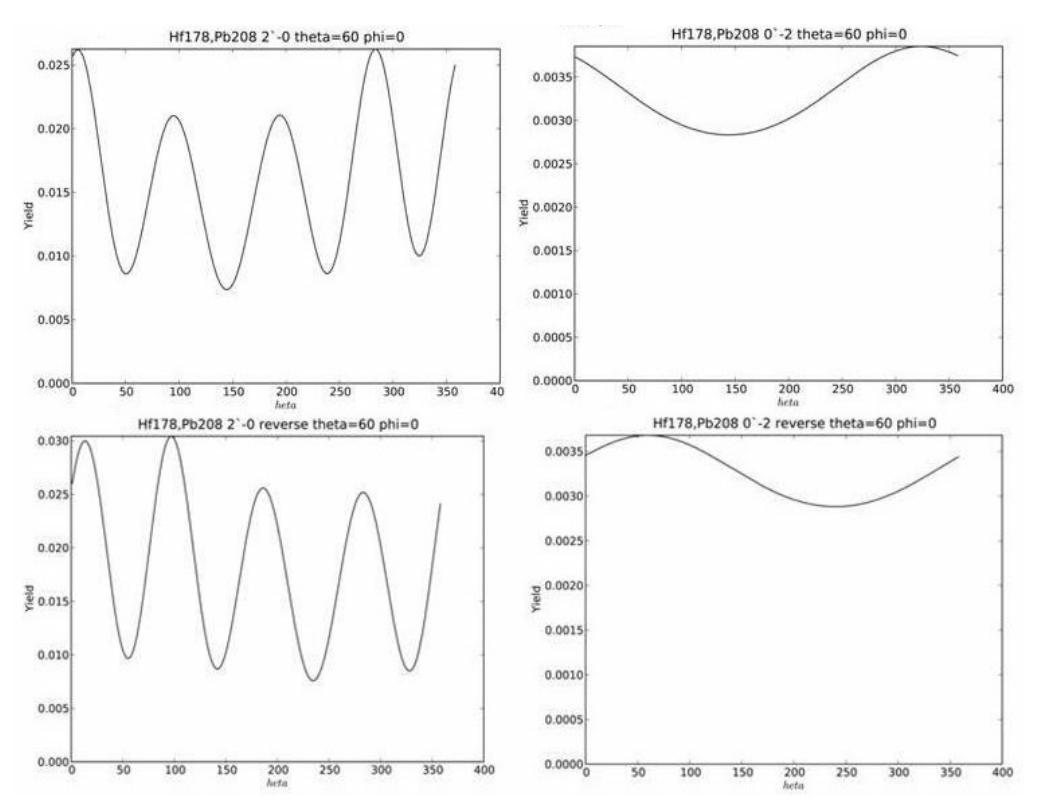
\includegraphics[max width=\textwidth]{2025_02_07_204a351db2d7f48b61ebg-054}
\end{center}

Figure 4.2: Upper row: Target excitation of ${ }^{208} \mathrm{~Pb}$ by a $890 \mathrm{MeV}{ }^{178} \mathrm{Hf}$ beam scattered at $\theta_{\text {proj }}=60^{\circ}$. Lower row: Projectile excitation of a $890 \mathrm{MeV}{ }^{178} \mathrm{Hf}$ beam scattered at $\theta_{\text {proj }}=60^{\circ}$ by a ${ }^{208} \mathrm{~Pb}$ target. Left column: shows a $2^{+}$state at 1.175 MeV decaying to the $0^{+}$ground state. Right column: shows a $1.0 \mathrm{MeV} 0^{+}$state decaying to the ground-band $2^{+}$state. The calculated yields are plotted versus $\theta_{\gamma}$ which is measured with respect to the incident beam direction. The deorientation effect has been switched off.

This implies that the $\rho_{k, \kappa}$ are real for $k+\kappa$ even, and imaginary for $k+\kappa$ negative. As a consequence the angular distribution of deexcitation $\gamma$-rays following excitation by projectile scattering at an angle $\theta_{L a b}^{\text {projecile }}$ has the symmetry axis along the major axis of the classical hyperbolic scattering orbit.

For inelastic scattering the scattered projectile mass is unchanged, and for heavy-ion Coulomb excitation the excitation energy is negligible compared with the incident beam energy. Therefore, to a good approximation the target recoils along and in the negative direction of the major axis of the hyperbola. As a consequence, to a good approximation, in the emitting nucleus frame of reference the symmetry axis of the $p-\gamma$ ray angular correlation is along the target recoil direction for both target or projectile excitation.

The relativistic angular distribution correction due to photon emission by a moving emitter is along the target recoil direction for target excitation and thus the symmetry of the angular correlation along the major axis of the hyperbolic orbit is retained for target excitation. By contrast, for projectile excitation the relativistic forward focussing is along the projectile direction which is very different from the symmetry axis of the angular distribution. That is, for projectile excitation the relativistic transformation of the $\gamma$ ray angular correlation destroys the symmetry about the major axis of the hyperbola. Thus for projectile excitation only the mirror symmetry about the scattering plane remains.

The alignment of the symmetry axis along the direction of the major axis of the hyperbolic orbit, which is aligned with the target recoil, and the forward focussing due to the relativistic transformation from the moving emitter frame to laboratory frame both are illustrated in Figure 4.2. Two such transitions were used in Gosia simulations assuming a $890 \mathrm{MeV}{ }^{178} \mathrm{Hf}$ beam scattered at $\theta_{\text {proj }}=60^{\circ}$ by a ${ }^{208} \mathrm{~Pb}$ target that excites a $2^{+}$state at 1175 keV resulting in the usual quadrupole radiation pattern in the recoil frame, and a $0^{+}$ state at 1000 keV that has an isotropic angular distribution in the recoil frame. The deorientation effect was switched off to emphasize the angular correlation. The quadrupole radiation pattern in the plots shown in the left-hand column emphasize the symmetry axis, whereas the plots in the right-hand column emphasize the effect of the Lorentz boost. The upper row figures show target excitation of ${ }^{208} \mathrm{~Pb}$. Figure 4.2 upper-left shows that the minimum of the $\gamma$ angular correlation along the symmetry axis is at $\theta_{\text {target }}=-36^{\circ}=324^{\circ}$ which is the correct direction, that is, along the target recoil direction. Figure 4.2 upper-right shows that the relativistic forward focussing also is along this target recoil direction as expected. As a consequence the two forward peaks shown in Figure 4.2 left are equally strong while the two backward direction peaks are\\
equally weak. The lower row figures show the angular distributions for projectile excitation, assuming the same kinematics. Figure 4.2 lower-left shows that the symmetry axis is calculated in the correct direction, that is, $\theta_{\text {target }}=-36^{\circ}=324^{\circ}$. However figure 4.2 lower-left shows that the intensity of the second peak at around $100^{\circ}$ is much stronger than the third peak in contrast to the case shown in for target excitation. That is, the relativistic transformation produces a significant asymmetry. Figure 4.2 lower-right shows that the relativistic forward focussing maximum now occurs in the direction of the recoiling excited projectile $\theta_{\text {proj }}=60^{\circ}$ which is very different from what is shown in Figure 4.2 upper-right for target excitation. Thus for normal kinematics the $p-\gamma$ angular correlations for both target and projectile excitation have the same symmetry axis but the angular distributions are very different. The general symmetry properties of the $p-\gamma$ angular correlation can be useful when designing experiments.

\section*{Chapter 5}
\section*{Kinematics, Coulomb trajectory, and energy loss}
Design and analysis of Coulomb excitation experiments require a detailed knowledge of the reaction kinematics, the Coulomb trajectory, and the energy loss of the incident and recoiling ions. This chapter reviews these three technical issues.

\subsection*{5.1 Kinematics for inelastic scattering}
This section reproduces the formulae [ALD75] necessary for handling inelastic scattering as well as calculation of energy loss. The semiclassical approximation is applicable for Coulomb excitation at incident energies below the Coulomb barrier allowing use of the classical approximation for two-body scattering kinematics. Consider the centre-of-mass to laboratory transformation using the velocity vectors and angles defined in Fig 5.1. Initially the target is assumed to be at rest and the projectile velocity is given by


\begin{equation*}
v_{i}=\sqrt{\frac{2 E_{P}}{m_{P}}} \tag{5.1}
\end{equation*}


where $E_{P}$ is the incident bombarding energy.

\subsection*{5.1.1 Velocities}
The initial velocities in the laboratory frame are taken to be

$$
\begin{array}{lll}
w_{P} & =v_{i} & \text { (Initial Lab velocities) } \\
w_{T} & =0 &
\end{array}
$$

The final velocities in the laboratory frame after the inelastic collision are

$$
w_{P}^{\prime}
$$

(Final Lab velocities)

In the centre-of-mass coordinate system the initial velocities are


\begin{align*}
u_{P} & =v_{i} \frac{m_{T}}{m_{P}+m_{T}} \\
u_{T} & =v_{i} \frac{m_{P}}{m_{P}+m_{T}} \tag{5.2}
\end{align*}


\begin{center}
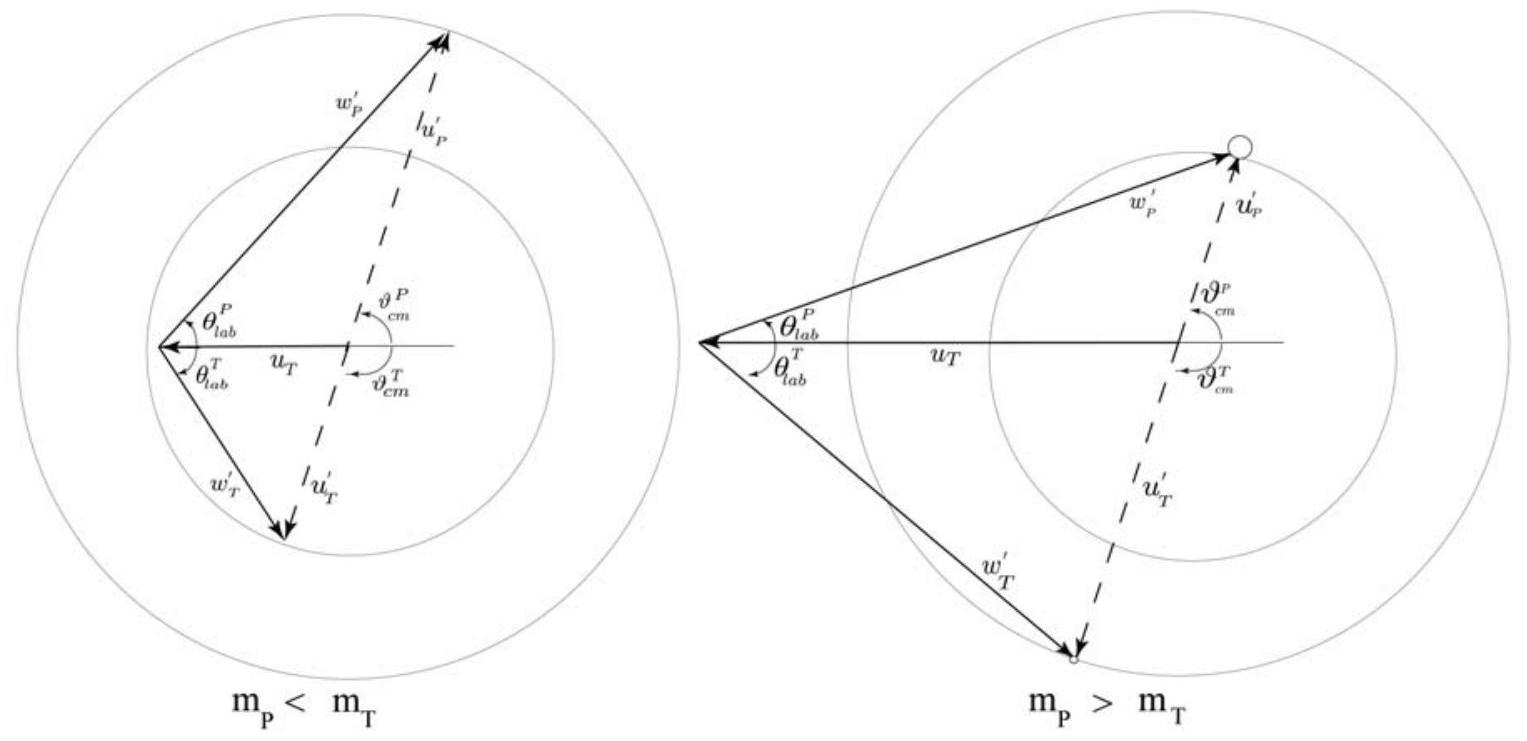
\includegraphics[max width=\textwidth]{2025_02_07_204a351db2d7f48b61ebg-058}
\end{center}

Figure 5.1: Vector hodograph of the scattered projectile and target velocities for a projectile, with incident velocity $v_{i}$, that is elastically scattered by a stationary target body. The circles show the magnitude of the projectile and target body final velocities in the centre of mass. The centre-of-mass velocity vectors are shown as dashed lines while the laboratory vectors are shown as solid lines. The left hodograph shows normal kinematics where the projectile mass is less than the target mass. The right hodograph shows inverse kinematics where the projectile mass is greater than the target mass.

The final centre-of-mass velocities after the inelastic collision are


\begin{align*}
u_{P}^{\prime} & =\frac{m_{T}}{m_{P}+m_{T}} \sqrt{\frac{2}{m_{P}} \tilde{E}} \\
u_{T}^{\prime} & =\frac{m_{P}}{m_{P}+m_{T}} \sqrt{\frac{2}{m_{P}} \tilde{E}} \tag{5.3}
\end{align*}


where


\begin{equation*}
\tilde{E}=E_{P}-\Delta E\left(1+\frac{m_{P}}{m_{T}}\right) \tag{5.4}
\end{equation*}


and $\Delta E$ is the excitation energy of the excited state. Note that the $Q$-value equals $-\Delta E$.

\subsection*{5.1.2 Angles}
The angles of the scattered recoils in the laboratory frame are written as

$$
\begin{gathered}
\theta_{l a b}^{P} \\
\theta_{l a b}^{T}
\end{gathered}
$$

(Final laboratory angles)\\
and in the centre-of-mass frame

$$
\begin{aligned}
\vartheta_{c m}^{P} & =\vartheta \\
\vartheta_{c m}^{T} & =\pi-\vartheta
\end{aligned}
$$

(Final CM angles)\\
where $\vartheta$ is the centre of mass scattering angle.\\
From Figure 5.1 it can be seen that angle relations between the laboratory and CM frames are connected by


\begin{equation*}
\frac{\sin \left(\vartheta_{c m}^{P}-\theta_{l a b}^{P}\right)}{\sin \theta_{l a b}^{P}}=\frac{m_{P}}{m_{T}} \sqrt{\frac{E_{P}}{\tilde{E}}} \equiv \tau \tag{5.5}
\end{equation*}


where


\begin{equation*}
\tau=\frac{m_{P}}{m_{T}} \frac{1}{\sqrt{1-\frac{\Delta E}{E_{P}}\left(1+\frac{m_{P}}{m_{T}}\right)}} \tag{5.6}
\end{equation*}


Equation 5.5 can be rewritten as


\begin{equation*}
\tan \theta_{l a b}^{P}=\frac{\sin \vartheta_{c m}^{P}}{\cos \vartheta_{c m}^{P}+\tau} \tag{5.7}
\end{equation*}


Another useful relation from equation 5.5 gives the centre of mass scattering angle in terms of the laboratory scattering angle.


\begin{equation*}
\vartheta_{c m}^{P}=\sin ^{-1}\left(\tau \sin \theta_{l a b}^{P}\right)+\theta_{l a b}^{P} \tag{5.8}
\end{equation*}


This gives the difference in angle between the laboratory scattering angle and the centre-of-mass scattering angle. Be careful with this relation since $\vartheta_{l a b}^{P}$ is two-valued for inverse kinematics corresponding to the two possible signs for the solution.

The angle relations between the laboratory and centre-of-mass frames for the recoiling target nucleus are connected by


\begin{equation*}
\frac{\sin \left(\vartheta_{c m}^{T}-\theta_{l a b}^{T}\right)}{\sin \theta_{l a b}^{T}}=\sqrt{\frac{E_{P}}{\tilde{E}}} \equiv \tilde{\tau} \tag{5.9}
\end{equation*}


That is


\begin{equation*}
\vartheta_{c m}^{T}=\sin ^{-1}\left(\tilde{\tau} \sin \theta_{l a b}^{T}\right)+\theta_{l a b}^{T} \tag{5.10}
\end{equation*}


where


\begin{equation*}
\tilde{\tau}=\frac{1}{\sqrt{1-\frac{\Delta E}{E_{P}}\left(1+\frac{m_{P}}{m_{T}}\right)}} \tag{5.11}
\end{equation*}


Note that $\tilde{\tau}$ is the same under interchange of the two nuclei at the same incident energy/nucleon, and that $\tilde{\tau}$ is always larger than or equal to unity. For elastic scattering $\tilde{\tau}=1$ which implies that

$$
\theta_{l a b}^{T}=\frac{1}{2}(\pi-\vartheta)
$$

(Recoil lab angle for elastic scattering)\\
The target recoil equation 5.9 can be rewritten as

$$
\tan \theta_{l a b}^{T}=\frac{\sin \vartheta_{c m}^{T}}{\cos \vartheta_{c m}^{T}+\tilde{\tau}}
$$

(Target lab to CM angle conversion)

Figure 5.2 shows the dependence of the projectile and target scattering angles in the laboratory frame as a function of centre-of-mass scattering angle for the Coulomb scattering of ${ }^{104} \mathrm{Pd}$ by ${ }^{208} \mathrm{~Pb}$, that is, for a mass ratio of 2.0. Both normal and inverse kinematics are shown at the same bombarding energy of $4.3 \mathrm{MeV} /$ nucleon for elastic scattering and for inelastic scattering with $\Delta E=5 \mathrm{MeV}$, that is, a $Q$-value of -5 MeV .

Since $\sin \left(\vartheta_{c m}^{T}-\theta_{l a b}^{T}\right) \leq 1$ then equation 5.9 implies that $\tilde{\tau} \sin \theta_{l a b}^{T} \leq 1$. Since $\tilde{\tau}$ is always larger than or equal to unity there is a maximum scattering angle in the laboratory frame for the recoiling target nucleus given by


\begin{equation*}
\sin \theta_{\max }^{T}=\frac{1}{\tilde{\tau}} \tag{5.12}
\end{equation*}


For elastic scattering $\theta_{l a b}^{T}=\sin ^{-1}\left(\frac{1}{\tilde{\tau}}\right)=90^{\circ}$ since $\tilde{\tau}=1$ for both a $447 \mathrm{MeV}{ }^{104} \mathrm{Pd}$ beam scattered by a ${ }^{208} \mathrm{~Pb}$ target, and the inverse of $894 \mathrm{MeV}{ }^{208} \mathrm{~Pb}$ bombarding ${ }^{104} \mathrm{Pd}$. A $Q$-value of -5 MeV gives $\tilde{\tau}=1.0085$ which implies a maximum scattering angle of $\theta_{\text {lab }}^{T}=82.558^{\circ}$ for both a $447 \mathrm{MeV}{ }^{104} \mathrm{Pd}$ beam scattered by a ${ }^{208} \mathrm{~Pb}$ target and the inverse of $894 \mathrm{MeV}{ }^{208} \mathrm{~Pb}$ bombarding ${ }^{104} \mathrm{Pd}$. As a consequence there are two solutions for $\vartheta_{c m}^{T}$ for any allowed value of $\theta_{l a b}^{T}$ as illustrated on the right in figure 5.2.

Since $\sin \left(\vartheta_{c m}^{P}-\theta_{l a b}^{P}\right) \leq 1$ then equation 5.5 implies that $\tau \sin \theta_{l a b}^{P} \leq 1$. For a $447 \mathrm{MeV}{ }^{104} \mathrm{Pd}$ beam scattered by a ${ }^{208} \mathrm{~Pb}$ target $\frac{m_{P}}{m_{T}}=0.50$, thus $\tau=0.5$ for elastic scattering which implies that there is no upper bound to $\theta_{l a b}^{P}$. This leads to a one-to-one correspondence between $\theta_{l a b}^{P}$ and $\vartheta_{c m}^{P}$ for normal kinematics.\\
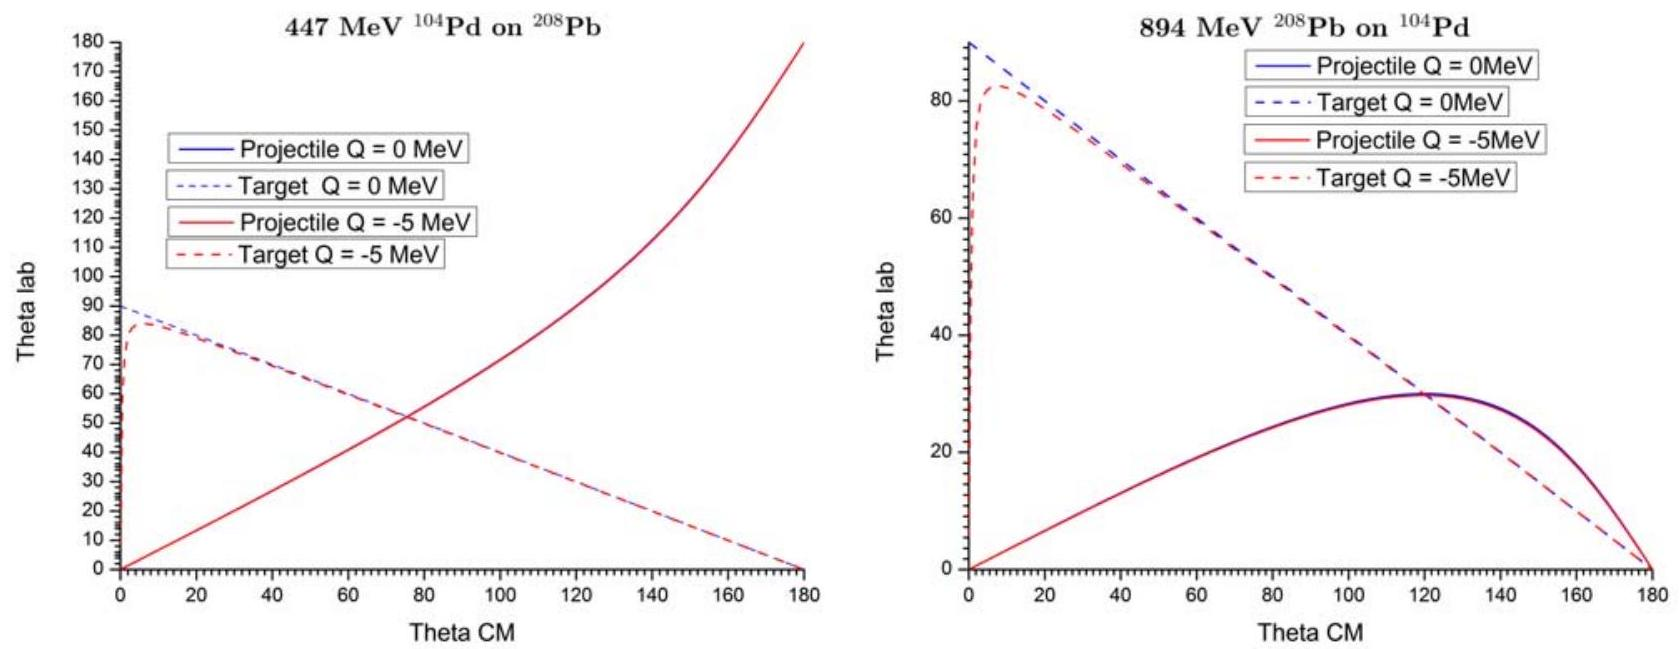
\includegraphics[max width=\textwidth, center]{2025_02_07_204a351db2d7f48b61ebg-060}

Figure 5.2: The kinematic correlation of the laboratory and centre-of-mass scattering angles of the recoiling projectile and target nuclei for scattering of $4.3 \mathrm{MeV} /$ nucleon ${ }^{104} \mathrm{Pd}$ on ${ }^{208} \mathrm{~Pb}$ (left) and $4.3 \mathrm{MeV} /$ nucleon ${ }^{208} \mathrm{~Pb}$ on ${ }^{104} \mathrm{Pd}$ (right). The projectile scattering angles are shown by solid lines while the recoiling target angles are shown by dashed lines. The blue curves correspond to elastic scattering $Q=0$, while the red curves correspond to inelastic scattering with $Q=-5 \mathrm{MeV}$.

In contrast, the projectile has a maximum scattering angle in the laboratory frame for inverse kinematics since $\frac{m_{P}}{m_{T}}=2.0$ leading to $\tau=2$ for elastic scattering and an upper bound to $\theta_{\text {lab }}^{P}$ given by


\begin{equation*}
\sin \theta_{\max }^{P}=\frac{1}{\tau} \tag{5.13}
\end{equation*}


In addition to a maximum value for $\theta_{l a b}^{P}$, when $\tau>1$ there are two solutions for $\vartheta_{c m}^{P}$ for any allowed value of $\theta_{\text {lab }}^{P}$. For example $894 \mathrm{MeV}{ }^{208} \mathrm{~Pb}$ bombarding ${ }^{104} \mathrm{Pd}$ leads to a maximum projectile scattering angle of $\theta_{l a b}^{P}=30.0^{\circ}$ for elastic scattering and $\theta_{l a b}^{P}=29.722^{\circ}$ for $Q=-5 \mathrm{MeV}$. Note that there is a small range of angles between $30.0^{\circ}$ and $29.722^{\circ}$ where population of the ground state can be observed but states with excitation energies above 5 MeV are not observed.

Figure 5.3 shows the correlation between $\theta_{l a b}^{P}$ and $\theta_{\text {lab }}^{T}$ for normal and inverse kinematics for the reaction discussed above. This illustrates the correlation observed when using the kinematic coincidence technique mentioned below.

\subsection*{5.1.3 Kinetic energies}
The initial total kinetic energy in the centre-of-mass frame is


\begin{equation*}
E_{c m}^{I n i t i a l}=E_{P} \frac{m_{T}}{m_{P}+m_{T}} \tag{5.14}
\end{equation*}


The final total kinetic energy in the centre-of-mass frame is


\begin{equation*}
E_{c m}^{\text {Final }}=E_{c m}^{\text {Initial }}-\Delta E=\tilde{E} \frac{m_{T}}{m_{P}+m_{T}} \tag{5.15}
\end{equation*}


where $\tilde{E}$ is defined by equation 5.4 .\\
In the laboratory frame the kinetic energies of the scattered projectile and recoiling target nucleus are\\
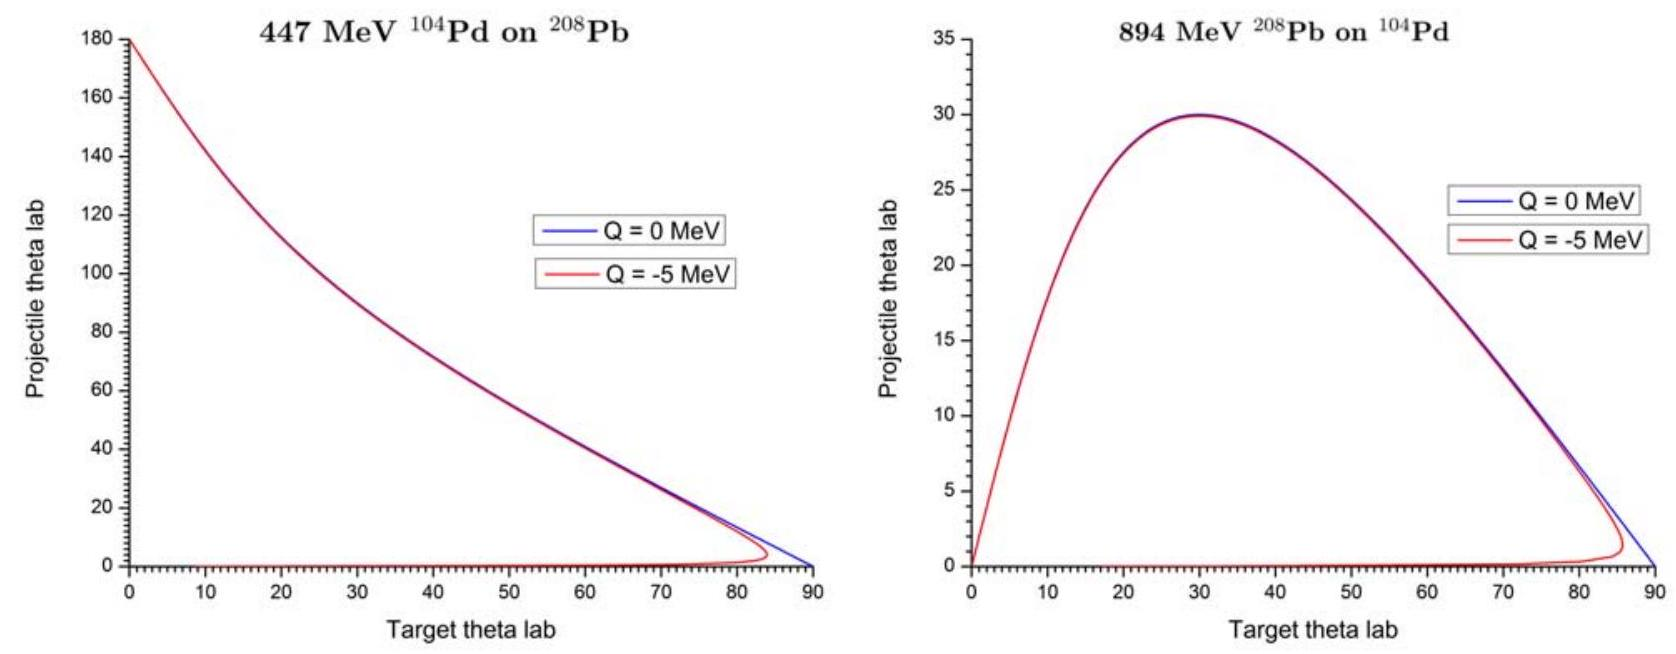
\includegraphics[max width=\textwidth, center]{2025_02_07_204a351db2d7f48b61ebg-061}

Figure 5.3: The kinematic correlation of the laboratory scattering angles for the recoiling projectile and target nuclei for scattering of a $4.3 \mathrm{MeV} /$ nucleon ${ }^{104} \mathrm{Pd}$ beam on ${ }^{208} \mathrm{~Pb}$ (left), and a $4.3 \mathrm{MeV} /$ nucleon ${ }^{208} \mathrm{~Pb}$ beam on ${ }^{104} \mathrm{Pd}$ (right). The blue curve is for elastic scattering, $Q=0$, and the red curve is for $Q=-5 \mathrm{MeV}$.\\
given by


\begin{align*}
E_{P}^{L a b} & =\left(\frac{m_{T}}{m_{P}+m_{T}}\right)^{2}\left(1+\tau^{2}+2 \tau \cos \vartheta_{c m}^{P}\right) \tilde{E}  \tag{5.16}\\
E_{T}^{L a b} & =\frac{m_{P} m_{T}}{\left(m_{P}+m_{T}\right)^{2}}\left(1+\tilde{\tau}^{2}+2 \tilde{\tau} \cos \vartheta_{c m}^{T}\right) \tilde{E} \tag{5.17}
\end{align*}


where $\vartheta_{c m}^{P}$ and $\vartheta_{c m}^{T}$ are the centre-of-mass scattering angles respectively for the scattered projectile and target nuclei.

Figure 5.4 shows the kinetic energies of the recoiling projectile and target nuclei as a function of laboratory scattering angle for both normal and inverse inelastic scattering of ${ }^{104} \mathrm{Pd}$ by ${ }^{208} \mathrm{~Pb}$ at $Q=-5.0 \mathrm{MeV}$. Note that good energy resolution is required to resolve the solutions at small scattering angles whereas the energy/nucleon, that is, velocities, are significantly different at these angles. The ${ }^{104} \mathrm{Pd}$ is cleanly separated from ${ }^{208} \mathrm{~Pb}$ at larger angles for both normal and inverse kinematics for this mass ratio. For inverse reactions the solutions having $\theta_{l a b}^{T} \approx 90^{\circ}$ correspond to small $\theta_{c m}^{P}$ which is not of interest for Coulomb excitation. Moreover, in this case the recoil energy of the target nucleus is too low to be detected because of target thickness or detector thresholds. Note that inverse kinematics focusses all the scattered nuclei into the forward hemisphere which reduces the required solid angle of the heavy-ion detectors. Moreover, for inverse reactions the recoil nuclei kinetic energies facilitate particle detection, and the energy losses of the backscattered projectiles in the target is not a problem.

\subsection*{5.1.4 Kinematic coincidence}
Knowledge of the recoil angle of the excited nucleus is required to define the hyperbolic trajectory needed for the Coulomb excitation calculation and also to make the appropriate Doppler correction for the detected deexcitation photon. The kinematic coincidence technique utilizes the angle-angle correlation, plus either the recoil energies or recoil velocities of the scattered reaction partners to identify unambiguously the reaction kinematics on an event-by-event basis. As mentioned above, the separation of the two solutions is enhanced using the recoil velocities, i.e. time of flight rather than recoil energies.

For normal kinematics $\tau<1$ there is a monotonic dependence of $\theta_{l a b}^{P}$ on $\theta_{l a b}^{T}$ except for inelastic scattering angles near $\theta_{l a b}^{P} \rightarrow 0$ where the target angle rapidly drops to zero. This forward-angle scattering solution for any target scattering angle is not of any consequence since it corresponds to target recoil energies that\\
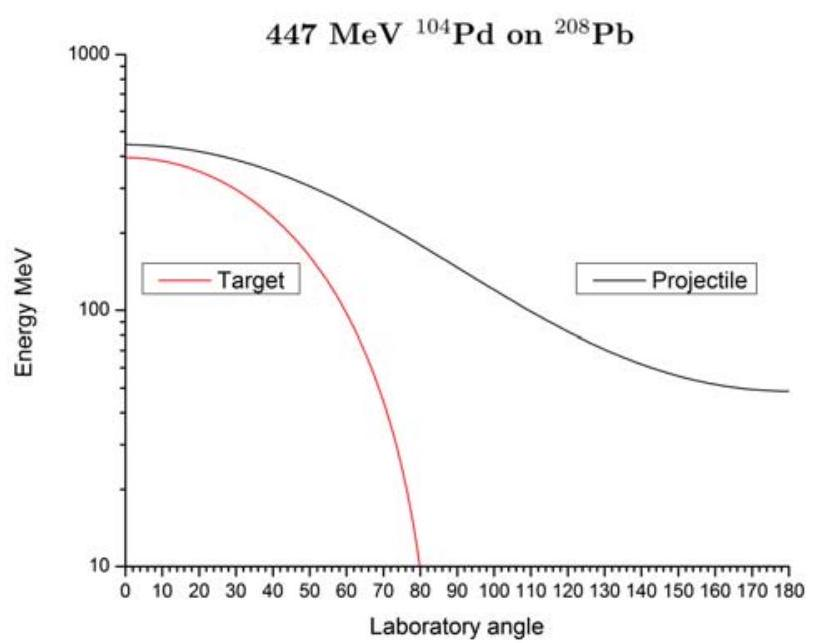
\includegraphics[max width=\textwidth, center]{2025_02_07_204a351db2d7f48b61ebg-062(1)}\\
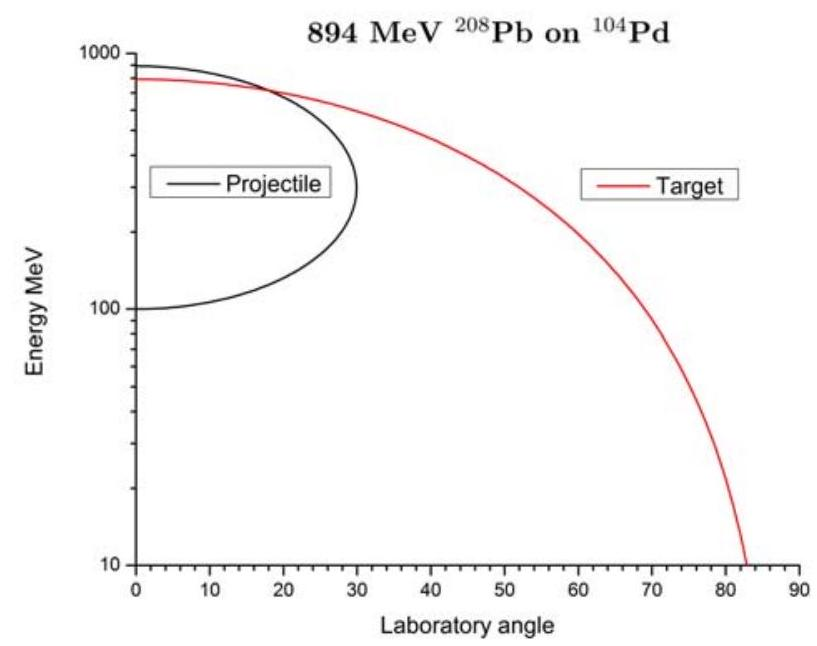
\includegraphics[max width=\textwidth, center]{2025_02_07_204a351db2d7f48b61ebg-062}

Figure 5.4: Recoil energies, in MeV , versus laboratory scattering angle. (Left) Scattering of $447 \mathrm{MeV}{ }^{104} \mathrm{Pd}$ by ${ }^{208} \mathrm{~Pb}$ for $Q=-5.0 \mathrm{MeV}$. (Right) Scattering of $894 \mathrm{MeV}{ }^{208} \mathrm{~Pb}$ on ${ }^{104} \mathrm{Pd}$ for $Q=-5.0 \mathrm{MeV}$.\\
are $<1 \mathrm{MeV}$ which usually are stopped in the target and are below the threshold for target ion detection. Even when the scattered ion $Z$ values are not measured, it is possible to unambiguously identify recoil ion masses by kinematic coincident detection with simultaneous measurement of the recoil-ion scattering angles plus either the recoil ion velocities or recoil energies.

For inverse kinematics, $\tau>1$ the angle-angle correlation is two valued both for projectile and target recoil angles as illustrated in Figure 5.3. For inelastic scattering the kinematic curve is energy dependent which can result in problems when using moderately thick targets. Fortunately the most forward-angle inelastic scattering in the centre-of-mass frame corresponds to a segment of the curve close to the abscissa for which the recoiling target nuclei have kinetic energies which normally are below the recoil-ion detection threshold. Thus for target-ion detection there is a one-to-one correspondence between scattering angle and target recoil angle. However, there are two kinematic solutions for a given projectile recoil angle. Detection of both the recoiling projectile and target nuclei in kinematic coincidence unambiguously identifies the centre-of-mass scattering angles and recoil ion masses eliminating the problems with two-valued solutions that can occur when only one scattered partner is detected as discussed in section 6.4.

\subsection*{5.1.5 Solid angles}
The lab solid angles for the scattered projectile and target are taken to be $d \omega_{P}$ and $d \omega_{T}$ respectively, while the centre-of-mass solid angles are $d \Omega_{P}$ and $d \Omega_{T}$ respectively. The Jacobian relating the solid angles is


\begin{align*}
& \frac{d \omega_{P}}{d \Omega_{P}}=\left(\frac{\sin \theta_{l a b}^{P}}{\sin \vartheta_{c m}^{P}}\right)^{2}\left|\cos \left(\vartheta_{c m}^{P}-\theta_{l a b}^{P}\right)\right|  \tag{5.18}\\
& \frac{d \omega_{T}}{d \Omega_{T}}=\left(\frac{\sin \theta_{l a b}^{T}}{\sin \vartheta_{c m}^{T}}\right)^{2}\left|\cos \left(\vartheta_{c m}^{T}-\theta_{l a b}^{T}\right)\right| \tag{5.19}
\end{align*}


\subsection*{5.2 Semiclassical Coulomb trajectory}
The semiclassical Coulomb trajectory is perturbed by the loss of kinetic energy due to inelastic excitation. States up to 7 MeV in excitation energy are observed in modern Coulomb excitation experiments and these high excitation energies can lead to a significant perturbation of the semiclassical trajectory. Each semiclassical calculation is performed for one specific hyperbolic trajectory which is uniquely related to the\\
centre-of-mass scattering angle $\theta_{c m}$ by the orbit eccentricity $\epsilon=\frac{1}{\sin \frac{\theta_{c m}}{2}}$. Section 3.4 described how the symmetrized orbit parameter approach can reasonably well account for the first-order perturbation of the Coulomb trajectory in the centre-of-mass coordinate frame.

In addition to the above correction, a kinematic correction is required to account for the fact that measurements are performed for the recoiling scattered nuclei detected over a range of laboratory scattering angles, and not for a range of centre-of-mass scattering angles assumed by theoretical calculations of the reaction mechanism. Section 5.1 .2 showed that the transformation from the laboratory to centre-of-mass angles for the scattered projectile depends on the parameter $\tau$, defined in equation 5.6 , and similarly for the recoiling target nucleus by the parameter $\tilde{\tau}$ defined in equation 5.11. Both $\tau$ and $\tilde{\tau}$ depend on the $Q$ value, and for $Q \neq 0$, they also depend on bombarding energy. As a consequence the centre-of-mass scattering angle, $\theta_{c m}$, and corresponding Coulomb trajectory, depend on the bombarding energy and $Q$ value of the state chosen to specify the centre-of-mass trajectory. The semiclassical Coulomb trajectory used by Gosia is for the state selected by the Gosia input $N C M$ in the control sub-option $C O N T$. The default value is $N C M=2$.

The choice of $N C M$ has three effects.\\
(1) The Jacobian for the laboratory to centre-of-mass transformation depends on $N C M$ via the $Q$-value.\\
(2) The cross section depends as the fourth power of the eccentricity $\epsilon=\frac{1}{\sin \frac{\theta_{c m}}{2}}$ which, for a given laboratory scattering angle, depends on $N C M$.\\
(3) The interaction time depends on the recoil ion velocity which is a function of $N C M$.

Note that the above discussion of the dependence of the centre-of-mass scattering angle on $Q$-value at a given laboratory scattering angle is a consequence of the elementary classical mechanics of two-body scattering. Calculations of the reaction mechanism invariably are performed in the centre-of-momentum frame, which also is the centre-of-mass frame for non-relativistic mechanics, whereas measurements are performed at a specific range of laboratory scattering angles. The important point is that the transformation between the laboratory frame and the centre-of-mass frame depends on the $Q$ value, and this is independent of whether the calculation of the reaction mechanism is a complicated fully quantal reaction calculation, or the semiclassical approximation. The impact of the $Q$ value dependence of the laboratory to centre-of-mass transformation on the ratio of the measured and theoretical cross sections is elucidated by study of the derivatives $\frac{d \vartheta_{c m}}{d Q}$ for both the recoiling projectile and target nuclei as given below.

For detection of the projectile at a fixed laboratory scattering angle $\theta_{l a b}^{P}$ the rate of change of the centre-of-mass angle $\vartheta_{c m}^{P}$ with excitation energy $\Delta E$ is given by the derivative of equation 5.8


\begin{equation*}
\frac{d \vartheta_{c m}^{P}}{d \Delta E}=-\frac{d \vartheta_{c m}^{P}}{d Q}=\frac{r(r+1) \sin \theta_{l a b}^{P}}{2 E_{P}\left(\frac{r}{\tau}\right)^{3} \sqrt{\left(1-\tau^{2} \sin ^{2} \theta_{l a b}^{P}\right)}} \tag{5.20}
\end{equation*}


where


\begin{equation*}
r \equiv \frac{M_{P}}{M_{T}} \tag{5.21}
\end{equation*}


and $\tau$ is given by equation 5.6.\\
For detection of the recoiling target nucleus at a fixed laboratory scattering angle $\theta_{l a b}^{T}$ the rate of change of the centre-of-mass angle $\vartheta_{c m}^{T}$ with excitation energy $\Delta E$ is given by the derivative of equation 5.10 to be


\begin{equation*}
\frac{d \vartheta_{c m}^{T}}{d \Delta E}=-\frac{d \vartheta_{c m}^{T}}{d Q}=\frac{(r+1) \sin \theta_{l a b}^{T}}{2 E_{P}\left(\frac{1}{\tilde{\tau}}\right)^{3} \sqrt{\left(1-\tilde{\tau}^{2} \sin ^{2} \theta_{l a b}^{T}\right)}} \tag{5.22}
\end{equation*}


where $\tilde{\tau}$ is given by equation 5.11 .\\
Figure 5.5 plots the magnitude of the derivatives $\frac{d \vartheta_{c m}^{P}}{d Q}=-\frac{d \vartheta_{c m}^{P}}{d \Delta E}$ and $\frac{d \vartheta_{c m}^{T}}{d Q}=-\frac{d \vartheta_{c m}^{T}}{d \Delta E}$ in degrees $/ \mathrm{MeV}$ versus the laboratory angle for normal kinematics using $4.3 \mathrm{MeV} /$ nucleon ${ }^{104} \mathrm{Pd}$ scattered by ${ }^{208} \mathrm{~Pb}$ for $Q=-5 \mathrm{MeV}$, and for inverse kinematics with $4.3 \mathrm{MeV} /$ nucleon ${ }^{208} \mathrm{~Pb}$ scattered by ${ }^{104} \mathrm{Pd}$ for $Q=-5 \mathrm{MeV}$. Note that for the normal-kinematics reaction $\frac{d \vartheta_{c m}^{T}}{d Q}=-\frac{d \vartheta_{c m}^{T}}{d \Delta E} \rightarrow \infty$ for the recoiling target nucleus at $\theta_{l a b}^{T}=82.558^{\circ}$. For the inverse-kinematics reaction the derivatives go to infinity at both the scattering-angle maxima $\theta_{l a b}^{P}=29.722^{\circ}$ for the scattered projectile and at $\theta_{l a b}^{T}=82.558^{\circ}$ for the scattered target.\\
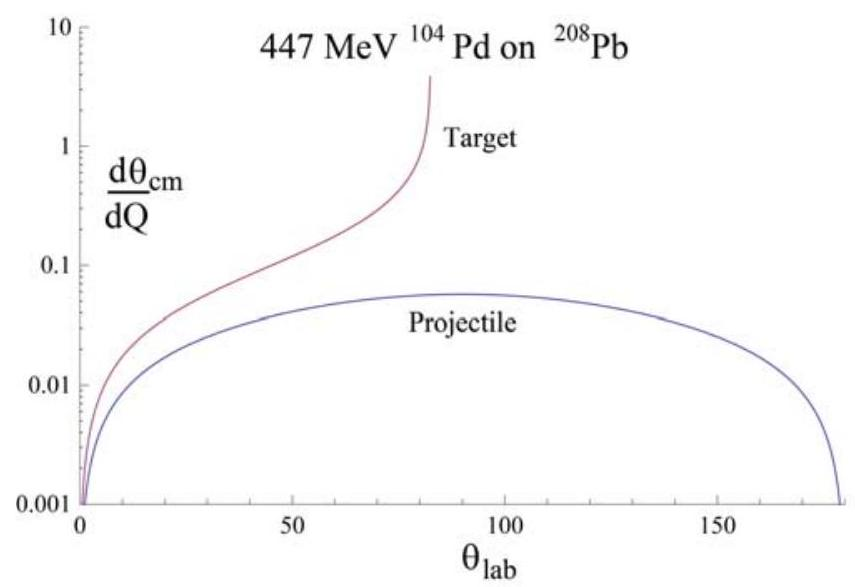
\includegraphics[max width=\textwidth, center]{2025_02_07_204a351db2d7f48b61ebg-064}\\
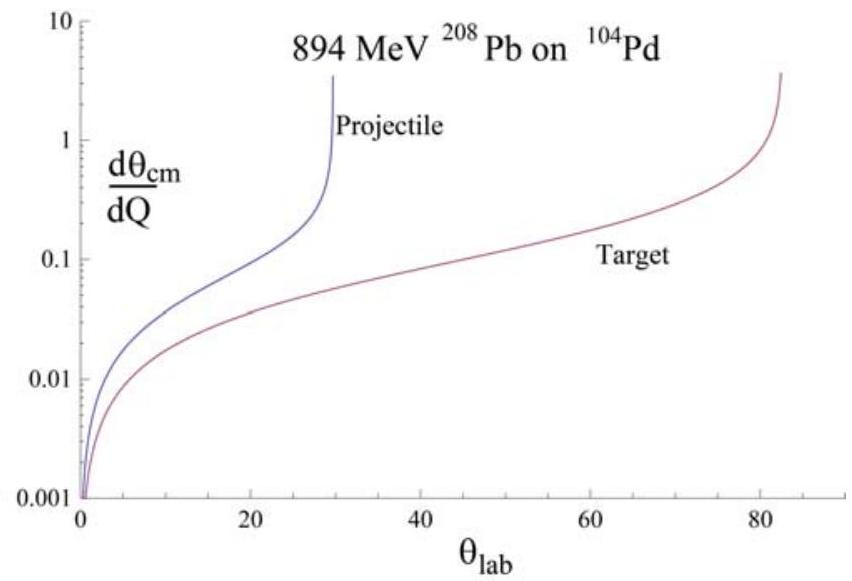
\includegraphics[max width=\textwidth, center]{2025_02_07_204a351db2d7f48b61ebg-064(1)}

Figure 5.5: The magnitude of the derivatives $\left|\frac{d \vartheta_{c m}^{P}}{d Q}\right|$ and $\left|\frac{d \vartheta_{c m}^{T}}{d Q}\right|$ in degrees/MeV versus the laboratory scattering angle for the recoiling projectile and target with normal kinematics and inverse kinematics for inelastic scattering of $4.3 \mathrm{MeV} /$ nucleon ${ }^{208} \mathrm{~Pb}$ by ${ }^{104} \mathrm{Pd}$ with $Q=-5 \mathrm{MeV}$. For normal kinematics the derivative goes to infinity at $\theta_{\text {lab }}^{T}=82.558^{\circ}$. For inverse kinematics the derivatives go to infinity at the angle maxima $\theta_{l a b}^{P}=29.722^{\circ}$ and $\theta_{l a b}^{T}=82.558^{\circ}$. The sign of the derivative $\frac{d \vartheta_{c m}^{P}}{d Q}$ is negative for angles $\vartheta_{c m}^{P}$ less than at the maximum of $\theta_{l a b}^{P}$ and positive for angles $\vartheta_{c m}^{P}$ that are larger than at the maximum of $\theta_{l a b}^{P}$. The sign of $\frac{d \vartheta_{c m}^{T}}{d Q}$ is positive. Note that the two-valued derivative curves overlap above and below the maximum recoil scattering angles in the laboratory frame.

The dependence of the centre-of-mass scattering angle $\vartheta_{c m}$ on $Q$-value, for a fixed laboratory scattering angle, implies that measurements at a given laboratory scattering angle require that the theoretical calculation of the reaction mechanism must be performed using a $Q$-value dependent range of $\vartheta_{c m}$ values. For example, the Coulomb trajectory that is used for a semiclassical calculation depends directly on $\vartheta_{c m}$ which is a function of the $Q$-value. It is interesting to investigate the implications of the sensitivity versus laboratory detection angles of the corresponding centre-of-mass scattering angle versus $Q$-value. For detection of the scattered projectile using inverse kinematics, where $r>1$, the rate of change of projectile centre-of-mass angle $\frac{d \vartheta_{c m}^{P}}{d \Delta E}$ becomes infinite when $\sin \theta_{l a b}^{P}=\frac{1}{\tau}$. This maximum projectile scattering angle occurs in the angular region that is of most interest for Coulomb excitation work. For detection of the scattered target recoil the rate of change $\frac{d \vartheta_{c m}^{T}}{d \Delta E}$ is infinite when $\sin \theta_{l a b}^{T}=\frac{1}{\tilde{\tau}}$ which occurs near $\theta_{l a b}^{T} \approx 90^{\circ}$ since $\tilde{\tau} \simeq 1$. Fortunately this latter case is not an especially valuable angle for Coulomb excitation since it corresponds to small scattering angles, $\vartheta_{c m} \rightarrow 0$, where the Coulomb excitation probability is small.

Figure 5.5 shows that for normal kinematics using heavy ions, the dependence of the derivative of $\theta_{c m}^{P}$ with $Q$-value is $<0.05^{\circ} / \mathrm{MeV}$. This effect is small and usually can be neglected when using heavy ions allowing one common hyperbolic trajectory to be used for a given laboratory scattering angle. However, for the recoiling target the shift in $\theta_{l a b}^{T}$ can be one to two orders of magnitude more sensitive at some scattering angles for a $Q$-value difference of 5 MeV . For the inverse reaction the $\frac{d \vartheta_{c m}^{P}}{d Q}$ sensitivity to laboratory scattering angle can exceed $1^{\circ} / \mathrm{MeV}$.

The impact of the $Q$-value dependence on the Coulomb trajectory is greatest for light nuclei because the spread in excitation energies of observed states is the largest, and the incident kinematic energy used for Coulomb excitation is the lowest. For example, Coulomb excitation of the 0.320 MeV state in ${ }^{11} \mathrm{Be}$ by a ${ }^{196} \mathrm{Pt}$ target resulted in the projectile derivative $\frac{d \vartheta_{c m}^{P}}{d Q}=0.044^{\circ} / \mathrm{MeV}$ at $26.9^{\circ}$ leading to the extracted $\mathrm{B}(\mathrm{E} 1)$ changing by $\sim 4.7 \%$ if the trajectory was calculated using the 1.685 MeV state trajectory rather than the trajectory for the 0.320 MeV state, and a $\sim 1 \%$ change occurred using the ground state trajectory. Another example is the inverse-kinematics scattering of $340 \mathrm{MeV}{ }^{120} \mathrm{Sn}$ by ${ }^{12} \mathrm{C}$, where the derivative for the projectile is, $\frac{d \vartheta_{c m}^{P}}{d Q}=1.87^{\circ} / \mathrm{MeV}$ at $\theta_{l a b}^{P}=5^{\circ}$. If the recoiling target angle $\theta_{l a b}^{T}$ is detected then the derivative $\frac{d \vartheta_{c m}^{T}}{d Q}$ for the target nucleus, ranges from $0.086^{\circ} / \mathrm{MeV}$ at $\theta_{l a b}^{T}=5^{\circ}$ to $4.74^{\circ} / \mathrm{MeV}$ at $\theta_{l a b}^{T}=69^{\circ}$. These large\\
angle shifts in $\theta_{c m}$ per $M e V$ in $Q$-value must be taken into account since they can result in the calculated cross sections changing by the order of $3 \%$ per MeV in $Q$-value for light nuclei, which is important when populating a wide range of excitation energies.

Like most theoretical calculations, the Gosia codes calculate the cross sections assuming a Coulomb trajectory corresponding to the centre-of-mass angle derived from the laboratory scattering angle at the $Q$ value of the state defined by the input $N C M$. The correct procedure is to calculate the cross section for each state at the measured laboratory scattering angles which results in a $Q$ dependent range of the corresponding centre-of-mass angles. This $Q$-value dependence of the laboratory to centre-of-mass transformation can be taken into account exactly by calculating separately the yield of each individual state, using the value of $N C M$ corresponding to that state, and then the yields from these separate calculations can be used to compute the experimental observables for fixed detector laboratory angles as described in chapter 6.6. Gosia has not been programmed to perform this procedure automatically when fitting matrix elements, thus if this procedure is required it must be performed externally by multiplying the measured yields by appropriate correction factors and then constructing by hand the corrected yields file \#4. See OP,CORR (chapter 7.4).

\subsection*{5.3 The "Rutherford" cross section}
It is useful to summarize the formula employed to calculated the so-called "Rutherford" cross section used in calculating the differential cross sections for inelastic scattering by Coulomb excitation. This incorporates the following two corrections from the case of elastic scattering.

\section*{1) Symmetrized orbit:}
The centre-of-mass hyperbolic trajectory is perturbed from that for elastic scattering due to the excitation energy of excited states in the interacting nuclei. This effect is accounted for by using a symmetrized orbit as described in chapter 3.4. This leads to the so-called "Rutherford" differential cross section given in millibarns/sr to be


\begin{equation*}
\left(\frac{d \sigma}{d \Omega}\right)_{c m}=1.29596 \frac{Z_{p}^{2} Z_{T}^{2}}{E_{s y m}^{2} \sin ^{4}\left(\frac{\vartheta_{c m}}{2}\right)} \tag{5.23}
\end{equation*}


The symmetrized centre-of-mass bombarding energy $E_{s y m}$ is defined to be


\begin{equation*}
E_{s y m}^{2}=E_{c m}^{\frac{3}{2}}\left(E_{c m}-\Delta E\right)^{\frac{1}{2}} \tag{5.24}
\end{equation*}


where


\begin{equation*}
E_{c m}=\frac{E_{P}}{\left(1+\frac{A_{P}}{A_{T}}\right)} \tag{5.25}
\end{equation*}


$\Delta E$ is the excitation energy of the excited state, and $E_{P}$ is the initial projectile energy in the laboratory frame. The energies $E_{s y m}, E_{c m}$, and $E_{P}$ all are in $M e V$ and the angles are in radians.\\
2) The centre-of-mass to laboratory frame transformation:

As discussed in chapter 5.2 , the transformation from the centre-of-mass to the laboratory frame is $Q$ value dependent as given by equations 5.18 and 5.19. Thus using equations 5.23 and 5.18 gives the projectile "Rutherford" differential cross section in the laboratory frame to be


\begin{equation*}
\sigma_{R}\left(\theta_{P}\right) \equiv\left(\frac{d \sigma}{d \Omega}\right)_{l a b}=\left(\frac{d \sigma}{d \Omega}\right)_{c m}\left(\frac{\sin \vartheta_{c m}^{P}}{\sin \theta_{l a b}^{P}}\right)^{2} \frac{1}{\left|\cos \left(\vartheta_{c m}^{P}-\theta_{l a b}^{P}\right)\right|} \tag{5.26}
\end{equation*}


where the projectile centre-of-mass angle is derived from the laboratory angle using equations 5.8 and 5.6


\begin{align*}
\vartheta_{c m}^{P} & =\sin ^{-1}\left(\tau \sin \theta_{l a b}^{P}\right)+\theta_{l a b}^{P}  \tag{5.8}\\
\tau & =\frac{m_{P}}{m_{T}} \frac{1}{\sqrt{1-\frac{\Delta E}{E_{P}}\left(1+\frac{m_{P}}{m_{T}}\right)}} \tag{5.6}
\end{align*}


In the semiclassical approximation the inelastic differential scattering cross section is given by multiplying $\sigma_{R}\left(\theta_{P}\right)$ by the Couomb excitation probability.

\subsection*{5.4 Energy loss}
Calculation of the populations of excited states depend strongly on the beam energy at each meshpoint and therefore the beam energy is used as the independent variable when integrating the cross sections over the projectile energy loss as it traverses the target. This requires accurate knowledge of the dependence of the rate of energy loss on ion velocity as the ion loses energy due to atomic and nuclear scattering processes in the target. The target thickness (and therefore the energy range over which the $\gamma$-decay cross sections must be calculated) and target uniformity are often poorly known, contributing additional error in the calculated yields.

Incident beam energies near the Coulomb barrier are typically used in Coulomb excitation experiments. In this bombarding-energy regime the electronic stopping is dominant, but complicated effects such as charge screening and crystal structure (steering/channeling) can be manifest. Nuclear stopping becomes significant at low beam energies for which the Coulomb excitation usually is insignificant.

The magnitudes of contributions to the energy loss due to target chemistry, steering, target density, etc. must all be evaluated in a complete model of stopping. Straggling, which requires a Monte-Carlo calculation, has an influence on the exit energy, and consequently the collision energy range that must be considered in the excitation probabilities for thicker targets. Even the crystal structure of the target, which is rarely known, affects the stopping power. Ziegler[ZIE08] gives a detailed description of the most important contributions to the total stopping power, as well as a history of the modeling of these effects. An example is for ${ }^{14} \mathrm{~N}$ ions at the Bohr velocity where the dependence of the electronic stopping power on target $Z_{T}$ value is irregular with factors of $\sim 2$ discontinuities at atomic shell closures as illustrated by Paul and Schinner [PAU03]. This irregularity is reduced for the higher velocity of heavy ions used for Coulomb excitation studies.

Figure 5.6 illustrates that there are significant discrepanies in the stopping power values derived from different compilations or the two utility codes elo and elast. These computer codes use models with parameters fit to the empirical data. The most reliable estimates are presumed to be given by the most recent compilations of Ziegler which are incorporated into his computer code SRIM[ZIE08]. The utility programs "elo" and "elast" both are based on a VAX/VMS Fortran program "eneloss.for", which is of unknown origin but presumably is based on part of the energy loss models used by SRIM. The SRIM predictions including nuclear stopping (solid black line) and excluding nuclear stopping (dashed black line) illustrate that nuclear stopping is unimportant at these beam velocities. SRIM gives a smooth energy dependence except for a slight discontinuity around $2 \mathrm{MeV} /$ nucleon. Ziegler[ZIE12] has explained that this discontinuity is due to merging of the high-energy stopping, which is the regime where the ion velocities are much faster than the target electrons, and the more complicated situation that exists at lower energies where the ion's velocity is comparable to the target electron velocities. The stopping-power compilation of Northcliffe and Schilling[NOR70] gives stopping powers that are significantly lower than the SRIM values for energies below $2 \mathrm{MeV} /$ nucleon which is a well-known problem, but they are in good agreement above this beam energy. The predictions of the two utility codes "elo" and "elast" deviate by as much as $\approx 15 \%$ from the SRIM values and have irregular energy dependence presumably due to unreliable interpolation as well as significantly underestimating the energy loss for lower velocity ions. While the SRIM source code is not public, there may be different versions of elo and elast in circulation. Thus it is recommended that the SRIM code be used. Figure 5.6 illustrates that the user must be cognizant of the significant discepancies that exist in available energy-loss compilations and computer codes.

The Gosia input file requires the user to supply stopping power data as $d E / d x\left(\mathrm{MeV} /\left(\mathrm{mg} / \mathrm{cm}^{2}\right)\right)$ as a function of projectile energy, where $E$ is the projectile energy, and $x$ is the position (depth) of the projectile in the target. Up to 20 stopping power meshpoints can be given, and Gosia interpolates between them using a cubic-spline function. A large number of stopping power points is recommended since the calculation time for interpolation is insignificant. Refer to the section on OP,INTI (chapters 7.12, 7.13). Following the integratedyield calculation, the cross sections are expressed in units of $\mathrm{mb}\left(\mathrm{mg} / \mathrm{cm}^{2}\right) / \mathrm{sr}$. This corresponds to the mean cross section integrated over the energy range given by the user, and the absolute cross section is obtained by dividing this cross section by the known target thickness. That is, the total yield can be expressed as an integral over the energy range, which can be translated directly into an absolute cross section by dividing by the known target thickness. Absolute cross sections in $m b$ for thick target experiments can only be calculated using the range of the stopped beam, which can be significantly less than the target thickness. The Rachel interface has several tools using SRIM or elast to automate calculation of the stopping power data for Gosia. This eliminates the need to iterate integrations outside of Gosia in order to find the exit energy for a thin\\
target, or the range for a thick target.\\
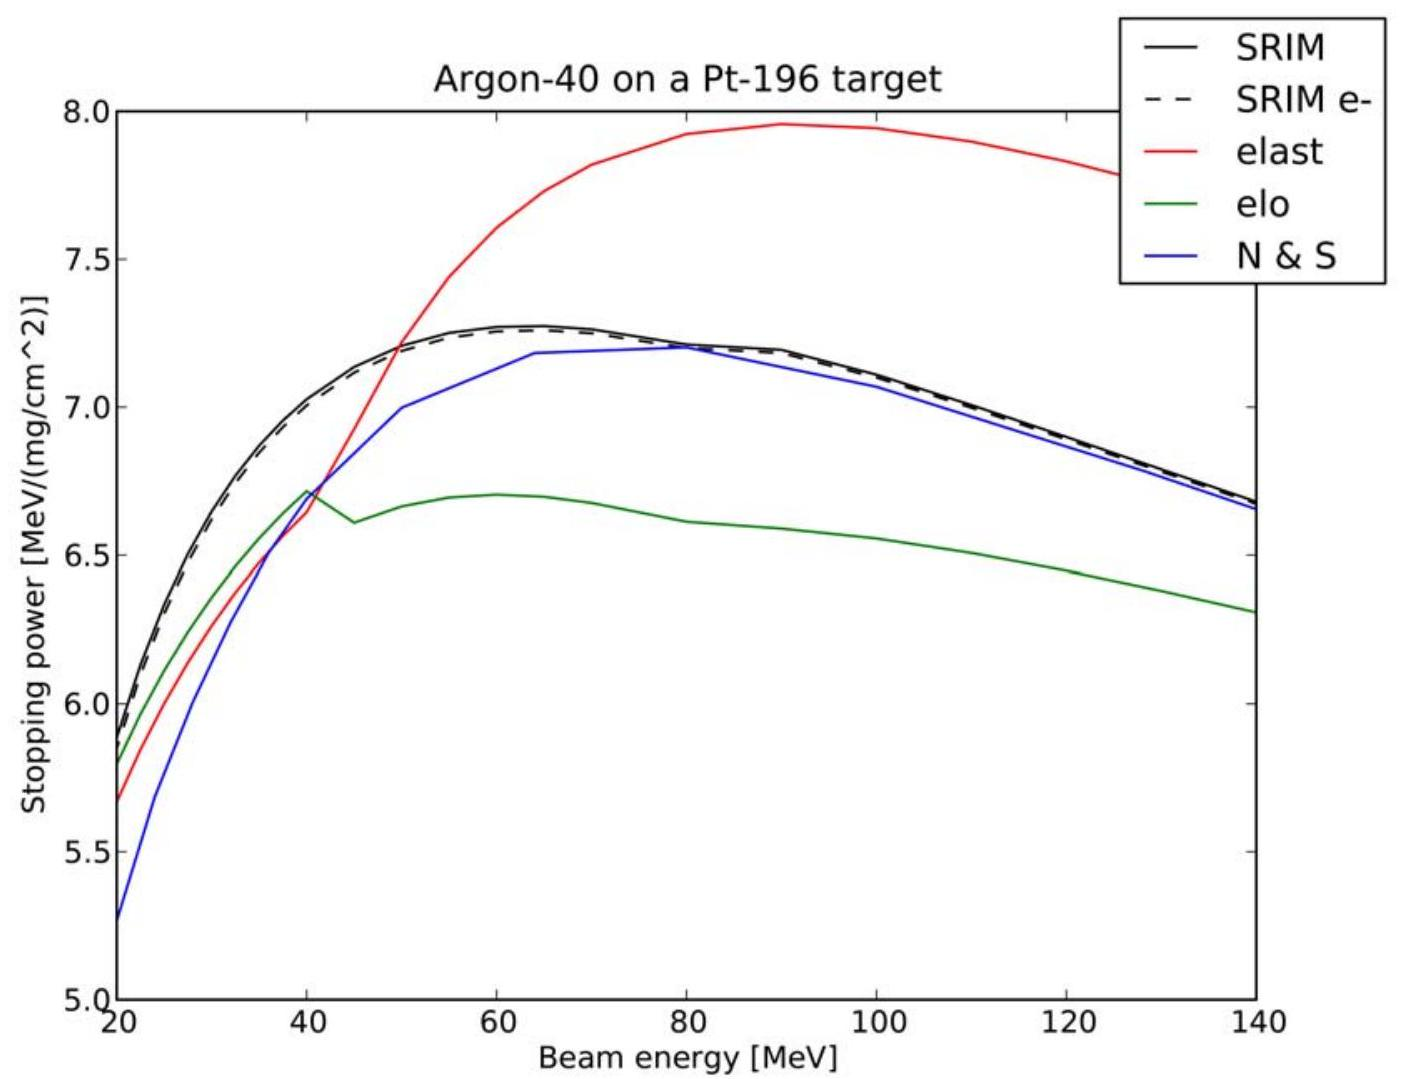
\includegraphics[max width=\textwidth, center]{2025_02_07_204a351db2d7f48b61ebg-067}

Figure 5.6: The calculated stopping power for an ${ }^{40} \mathrm{Ar}$ beam in ${ }^{196} \mathrm{Pt}$ is shown as a function of beam energy given by the 2011 version of the Ziegler code SRIM[ZIE08], Northcliffe and Schilling[NOR70], and the utility computer codes ELO and ELAST.

\section*{Chapter 6}
\section*{Numerical methods}
The code GOSIA is designed to perform various functions defined by a user-specified sequence of "options". In the simplest mode, GOSIA can be used to calculate the excitation probabilities, population, and statistical tensors of the levels, equation 4.1, thus providing an equivalent to the code COULEX. Activating the $\gamma$-ray decay module of the code extends this type of calculation to obtain the $\gamma$-ray yields for a single value of bombarding energy and scattering angle, as well as performing integration over specified ranges of the bombarding energy (due to the projectile energy loss in a target) and projectile scattering angle to reproduce real experimental conditions. These calculations require an input set of matrix elements treated as fixed data. The main purpose of GOSIA is, however, to fit the electromagnetic matrix elements to reproduce available experimental data. GOSIA can handle simultaneously experimental $\gamma$-ray yields (up to 48000 ) observed in 50 independent "logical experiments". Additional data, i.e. branching ratios (max. 50 ), lifetimes of the nuclear levels (max. 10), E2/M1 mixing ratios (max. 20) and previously measured $E \lambda$ matrix elements (max. 30) also may be included. All these data, and their experimental uncertainties, are used to construct a least-squares statistic, usually called $\chi^{2}$ or penalty function. The minimum of this statistic, treated as a function of matrix elements, defines the solution, while its distribution in the vicinity of the minimum determines the errors of fitted matrix elements. In the present version of the code, the investigated nucleus is described by a maximum of 99 energy levels, with the number of magnetic substates not exceeding 1200. The levels may be coupled with up to 999 matrix elements ( $E 1$ through $E 6$ and $M 1$, M2), any number of them allowed to be declared as the variables to be fitted. Memory limitations reduce this number in proportion to the quantity of input data required for a calculation which is case dependent.

As mentioned before, direct use of the full Coulomb excitation formalism to perform the minimization is out of the question due to the computer time necessary for repeated calculations. The mimimization can be accelerated using the approximation presented in chapter 6.2. A significant amount of time also can be saved if the recoil-velocity correction (4.5) is neglected. The effect of both replacing the full excitation formalism by the matrix approximation and neglecting the relativistic correction is only weakly dependent on the matrix elements, therefore it is feasible to introduce the "correction factors", that account for the differences between full and approximate calculations which are assumed to be independent of the fitted matrix elements. The minimization can be performed using primarily the fast, approximate formalism, with"fast-correction correction factors" refreshed by running the full calculation periodically. In addition, the Coulomb excitation fast approximation is applied only to $\Delta m=0$ and $\Delta m= \pm 1$ couplings, thus an effect of truncation of the number of magnetic substates being taken into account is also included in the correction factors, since this is not strongly dependent on the actual set of matrix elements.

Further acceleration of the fitting procedure is made possible by replacing the integration over experimentdependent scattering angle and bombarding energy ranges with a single calculation of the Coulomb excitation induced $\gamma$-ray yields assuming the mean values of the scattering angle and bombarding energy. This approximation also is not explicitly dependent on the fitted matrix elements, thus the difference between the integration procedure and the result of using the mean values of bombarding energy and scattering angle can be accounted for by introducing another set of correction factors, treated as constants. Actually, it is convenient to apply this correction to the experimental yields, i.e. to rescale the experimental data ac-\\
cording to the comparison of integrated and "mean yields". This is done initially using a starting set of matrix elements and the resulting "corrected experimental yields" are subsequently used as the experimental values for fitting (this procedure is presented in detail in Section 6.5). Thus, the fitting of matrix elements is performed using two levels of iteration - first, external, is to replace the experimental ranges of bombarding energy and scattering angle with the average values of these parameters, while second, internal, is the actual minimization of the least-squares statistic. After the convergence at the internal level is achieved, one should recalculate the correction to the experimental yields with the current set of matrix elements and repeat the minimization. Usually, for thin targets and not an excessively wide range of scattering angles, the second repetition of external iteration already results in negligible changes in the matrix elements found by the minimization. Even if no particle coincidences were required, it has been determined that only 2-3 recalculactions on the external level were necessary despite the integration over the full solid angle. This can be tested by checking that subsequent iterations result in no change in matrix elements.

Estimation of the errors of fitted matrix elements is a final step for the Coulomb excitation data analysis. This rather complicated procedure is discussed in Section 6.8. A Gosia option OP,SELE (SELECT) has been written to reduce the considerable computational effort required for this task using the information obtained during minimization. This information, preprocessed by OP,SELE, is fed back to the error routine. Optionally, the results of minimization and error runs can be used to evaluate quadrupole sum rules by a separate code SIGMA (Chapter 9).

The extraction of the matrix elements from experimental data requires many runs of GOSIA. During these runs, GOSIA creates and updates a number of disk files, containing the data needed to resume the analysis or to execute OP,SELE or SIGMA codes. The details of permanent file manipulation are presented in Chapter 10.

Relatively modest RAM requirements of GOSIA (about 1.5 MB ) are due to the sharing of the same memory locations by different variables when various options are executed and to replacing the multidimensional arrays (such as e.g. matrix elements) with catalogued vectors and associated logical modules. This sharing was introduced due to the limited computer memory available when GOSIA was developed in 1980. This extensive overlaying of the coding produced a complicated internal organization of GOSIA. The description of the code given in this chapter therefore will not attempt to account for its internal organization, which is heavily dependent on the sequence of options executed and, in general, of no interest to the user. Instead, it will concentrate on the algorithms used and the logic employed in GOSIA. The basic knowledge of the algorithms is essential since the best methods of using the code are strongly case-dependent, so much freedom is left to the user to choose the most efficient configurations according to the current needs.

All three codes- GOSIA, SIGMA and SELECT- are written in the standard FORTRAN77 to make their implementation on various machines as easy as possible. Full 64 bit accuracy is strongly recommended since the results can be untrustworthy when run using 32 bit accuracy.

\subsection*{6.1 Coulomb Excitation Amplitudes and Statistical Tensors}
The state of a Coulomb excited nucleus is fully described by the set of excitation amplitudes, $a_{I M}\left(M_{0}\right)$, defined by the solution of Eq. 3.20 at $\omega=\infty$, or, approximately, by the matrix expansion Eq. 6.14, used for minimization and error estimation. To set up the system of coupled-channel differential equations 3.20 it is necessary first to define the level scheme of an excited nucleus. Certainly, from a practical point of view, the level scheme should be truncated according to the experimental conditions in such a way that reasonable accuracy of the excitation amplitudes of the observed states is obtained with a minimum number of the levels included in the calculation. As a rule of thumb, two levels above the highest observed state in each collective band should be taken into account to reproduce a given experiment reliably. Truncation of the level scheme at the last observed level leads to an overestimation of the excitation probability of this level due to the structure of the coupled-channels system, equation 3.20, while including additional levels above, even if their position is only approximately known, eliminates this spurious effect.

The solution to the coupled-channels system, equation 3.20 should, in principle, involve all magnetic substates of a given state $\mid I>$, treated as independent states within a framework of the Coulomb excitation formalism. However, due to the approximate conservation of the magnetic quantum number in the coordinate system used to evaluate the Coulomb excitation amplitudes (as discussed in Chapter 3) it is practical to limit the number of the magnetic substates taken into account for each polarization of the ground state, $M_{0}$. In any case, the excitation process follows the "main excitation path", defined as a set of magnetic substates\\
having the magnetic quantum number equal to $M_{0}$, the remaining magnetic substates being of less and less importance as the difference between their magnetic quantum number and $M_{0}$ increases. The relative influence of the excitation of magnetic substates outside the main excitation path is experiment-dependent, therefore GOSIA allows the user to define the number of magnetic substates to be taken into account separately for each experiment. This choice should be based on the requested accuracy related to the quality of the experimental data, keeping in mind that reasonable truncation of the number of the magnetic substates involved in Coulomb excitation calculations directly reduces the size of the coupled-channels problem to be solved.

Theoretically the integration of the coupled differential equations 3.20 should be carried over the infinite range of $\omega$, which, practically, must be replaced with a finite range wide enough to assure the desired accuracy of the numerical solution. To relate the effect of truncating the $\omega$-range to the maximum relative error of the absolute values of the excitation amplitudes, $a_{c}$, the following criterion can be used to check that the integration of the collision functions is sufficently accurate:


\begin{equation*}
\frac{1}{4} \frac{\int_{-\infty}^{\infty} Q_{\lambda 0}(\epsilon=1, \omega) d \omega-\int_{-\omega}^{\omega_{\max }^{\max }} Q_{\lambda 0}(\epsilon=1, \omega) d \omega}{\int_{-\infty}^{\infty} Q_{\lambda 0}(\epsilon=1, \omega) d \omega} \leq a_{c} \tag{6.1}
\end{equation*}


where, as a worst case, the backscattering geometry $(\epsilon=1)$ is taken into account, thus $\Delta m \neq 0$ couplings vanish for electric excitations. There is no magnetic excitation for backscattering, as discussed in Chapter 3, moreover, the magnetic excitation is weak enough to be neglected at the excitation stage for any scattering angle, therefore only electric excitation is considered in this criterion. The factor $1 / 4$ is introduced in equation 6.1 to account for the further decrease of the importance of the excitation taking place at large $|\omega|$ due to the high-frequency oscillation introduced by the exponential term of equation 3.20. Using the normalization property of the collision functions:


\begin{equation*}
\int_{-\infty}^{\infty} Q_{\lambda \mu}(\epsilon=1, \omega) d \omega=1 \tag{6.2}
\end{equation*}


and the asymptotic, pure exponential form of collision functions for large $|\omega|$ one finally gets:


\begin{equation*}
\omega^{\max } \geq \alpha_{\lambda}-\frac{1}{\lambda} \ln a_{c} \tag{6.3}
\end{equation*}


where the values of $\alpha_{\lambda}$ can be found from the asymptotic form of the collision functions and are given in the table below, together with the resulting $\omega^{\max }$ assuming $a_{c}=10^{-5}$ which is the default value in GOSIA

Table 6.1: Maximum ranges $\omega^{\max }$ and asymptotic exponents

\begin{center}
\begin{tabular}{|c|c|c|}
\hline
multipolarity & $\alpha_{\lambda}$ & $\omega^{\max }$ for $\mathrm{a}_{c}=10^{-5}$ \\
\hline
E1/M2 & -.693 & 10.82 \\
\hline
E2/M3 & .203 & 5.96 \\
\hline
E3 & .536 & 4.37 \\
\hline
E4 & .716 & 3.59 \\
\hline
E5 & .829 & 3.13 \\
\hline
E6 & .962 & 2.88 \\
\hline
\end{tabular}
\end{center}

The range of integration over $\omega$ corresponding to a given accuracy level decreases with increasing multipolarity, as can be seen in Table 6.1. Following this observation, the coupling between energy levels corresponding to a given multipolarity is included in GOSIA only within the integration range assigned to this multipolarity, which is a time-saving feature in cases where many multipolarities have to be included. For $M \lambda$ couplings, neglected so far, the integration ranges have been set according to:


\begin{equation*}
\omega^{\max }(M \lambda)=\omega^{\max }(E(\lambda+1)) \tag{6.4}
\end{equation*}


The actual integration of the coupled-channel system of differential equations 3.20 is performed in GOSIA using the Adams-Moulton predictor-corrector method. According to this algorithm, first the predicted\\
solution $\bar{a}$ at $\omega+4 \Delta \omega$, based on a knowledge of the solution at $\omega+3 \Delta \omega$ and the derivatives $\bar{a}^{\prime}$ at four points, $\omega, \omega+\Delta \omega, \omega+2 \Delta \omega$ and $\omega+3 \Delta \omega$ is found using:


\begin{equation*}
\bar{a}(\omega+4 \Delta \omega)=\bar{a}(\omega+3 \Delta \omega)+\frac{\Delta \omega}{24}\left\{55 \bar{a}^{\prime}(\omega+3 \Delta \omega)-59 \bar{a}^{\prime}(\omega+\Delta \omega)+37 \bar{a}^{\prime}(\omega+\Delta \omega)-9 \bar{a}^{\prime}(\omega)\right\} \tag{6.5}
\end{equation*}


and then corrected by:


\begin{equation*}
\bar{a}(\omega+4 \Delta \omega)=\bar{a}(\omega+6 \Delta \omega)+\frac{\Delta \omega}{24}\left\{9 \bar{a}^{\prime}(\omega+4 \Delta \omega)+19 \bar{a}^{\prime}(\omega+3 \Delta \omega)-\overline{5} a^{\prime}(\omega+2 \Delta \omega)+a^{\prime}(\omega+\Delta \omega)\right\} \tag{6.6}
\end{equation*}


where the excitation amplitudes are once again treated as a vector and the prime symbolically denotes the differentiation with respect to $\omega$. The predicted solution is used to obtain the derivatives defined by the righthand side of 3.20 at $\omega+4 \Delta \omega$, employed to evaluate the corrector 6.6. Stepsize, $\Delta \omega$, is controlled on a basis of the comparison of the predicted and corrected solutions. The accuracy test parameter, $d$, is defined as $1 / 14$ of the absolute value of the maximum difference between the predicted and corrected excitation amplitudes at a current value of $\omega$. The stepsize is then halved if $d>a_{c}$ or doubled if $d<a_{c} / 50$. This procedure assures the adjustment of the stepsize according to the strength of the interaction and is performed every $n$ steps, $n$ being an adjustable parameter defined by the user ( $n=1$ is used as a default in GOSIA). The Adams-Moulton integration algorithm, with stepsize control, usually is faster than Runge-Kutta type methods, thus it has been employed in GOSIA despite some drawbacks. The most important drawback is when the interaction, defined by the left-hand side of 3.20 , is weak over most of the integration range, peaking only around some value of the independent variable. In this case, the stepsize will be subsequently doubled and can become excessively large when the strong interaction region is reached. Consequently, even though the loss of accuracy is detected, the overall accuracy of integration would be irretrievably lost. Note that convergence problems are more likely to occur for high excitation energy transitions, $>2.5 \mathrm{MeV}$ where the large adiabaticity parameter $\xi_{k n}$ in equation 3.20 leads to a rapid oscillation relative to the stepsize $\Delta \omega$. Fortunately for these large adiabaticities the excitation probabilities usually are below the experimental sensitivity of current experiments. The loss of accuracy for high adiabaticity transitions can be detected by checking the sum of excitation probabilities provided in the output of GOSIA. The recommended procedure, if the sum of probabilities differs significantly from unity, is to switch off the stepsize control for a given experiment using the INT switch of CONT suboption (see section 7.3) rather than decrease the accuracy parameter $a_{c}$. This is due to the fact that GOSIA uses the table of $Q_{l m}$ functions and hyperbolic functions with a tabulation step $\Delta \omega=0.03$ which defines the minimum stepsize of the integration independent of the accuracy requested, allowing the highest accuracy corresponding to $a_{c}=10^{-6}$. Increasing the requested accuracy control $a_{c}$ may exacerbate the problem by causing Gosia to read the $Q_{l m}$ function versus $\omega$ tables outside the boundaries for each multipole. The user should select the INT setting for the highest accuracy since the CPU time required is insignificant on modern computer systems.

Another drawback of the Adams-Moulton method, compared to the Runge-Kutta algorithm, is that Adams-Moulton algorithm is not self-starting, requiring the initial solutions at four points. This problem can be overcome by employing the Runge-Kutta algorithm to provide the starting values, then switching to the more efficient Adams-Moulton method (note that the same procedure is to be applied when the stepsize is changed, since restarting the integration with different stepsize requires the knowledge of the solution at new independent parameter intervals). The Runge-Kutta integration algorithm is used in the code COULEX[WIN65] to provide the starting solution for both the initialization of the integration and the changes of stepsize. In GOSIA the starting solutions are found using a first-order perturbation approach, valid at large values of $\omega$, using the asymptotic form of the collision functions. It is assumed that the ground state is connected to at least one excited state with $E 1, M 1$ or $E 2$ matrix elements. The initial excitation amplitudes then can be found as combinations of trigonometric and integral-trigonometric functions, the latter being evaluated using a rational approximation (given for example in [ABR72]). To fully eliminate switching to the Runge-Kutta algorithm, when changing the stepsize, the new starting values are evaluated using backward interpolation. This procedure is reliable enough to assure reasonable accuracy while considerably speeding up the integration.

The integration of the system 3.20 in principle should be repeated for each possible polarization of the ground state, $M_{0}$. However, the reflection symmetry in the plane of the orbit in the coordinate system used to evaluate the excitation amplitudes yields:


\begin{equation*}
a_{I m}\left(M_{o}\right)=(-1)^{\Delta \pi+I_{o}-I} a_{I-m}\left(-M_{o}\right) \tag{6.7}
\end{equation*}


where $\Delta \pi=0$ if there is no parity change between the ground state and a given excited state $\mid I>$, and $\Delta \pi=1$ otherwise. The symmetry relation 6.7 means one only has to solve the coupled-channel system 3.18 for the ground state polarizations $M_{0} \geq 0$, the solution of the coupled-channel system for $M_{0} \leq 0$ being defined by the relation 6.7. As mentioned before, due to the approximate conservation of the magnetic quantum number in the frame of coordinates used, one practically has to take into account only a limited subset of magnetic substates beyond the main excitation path. This explicitly means that if $n$ magnetic substates have been specified by the user to be included in the Coulomb excitation calculation, then for each excited state, $I$, and ground state polarization, $M_{0}$, GOSIA will catalog the magnetic substates according to the inequality:


\begin{equation*}
\min \left(I,-M_{0}+n\right) \geq m \geq \max \left(-I,-M_{0}-n\right) \tag{6.8}
\end{equation*}


which, by virtue of 6.7 , defines simultaneously a set of excitation amplitudes obtained with the inverse polarization of the ground state in a range given by:


\begin{equation*}
\max \left(-I, M_{0}-n\right) \leq m \leq \min \left(I, M_{0}+n\right) \tag{6.9}
\end{equation*}


allowing for the summation of excitation amplitudes to form a statistical tensor defined by 4.2 for $+M_{0}$ and $-M_{0}$ at the same time.

A special simplification of the solution of equation 3.20 occurs for the ground state spin equal to 0 (eveneven nuclei). In this case only $m \leq 0$ substates are explicitly included for numerical integration, the values of the excitation amplitudes and their derivatives for $m \geq 0$ are substituted during the integration using equation 6.7. Therefore, a separate setup of the system of coupled-channels equations 3.20 is constructed by GOSIA for even-even nuclei, resulting in the appreciable increase of the speed of the integration if $I_{0}=0$.

The statistical tensors $\rho_{k \chi}$ are evaluated first according to equation 4.2 in the coordinate system used to calculate the excitation amplitudes, then rotated to coordinate frame " $B$ ", shown in figure 4.1 , system, which is more convenient to describe the $\gamma$-deexcitation, as discussed in Chapter 4. This transformation is done using the rotation matrices according to equation 4.12. Rotated statistical tensors are treated as an interface between the Coulomb excitation and $\gamma$-deexcitation modules of the code, providing the complete information needed to calculate the $\gamma$-ray decay. These tensors can be calculated either using the full Coulomb excitation formalism or using the fast matrix approximation.

\subsection*{6.2 Approximate evaluation of the Coulomb excitation amplitudes}
Numerical integration of the system of differential equations 3.20 , over $\theta_{\text {scat }}, E_{\text {beam }}$ is time consuming. This is due to the requirement to solve the coupled-channels equations at each $\theta, E$ meshpoint. Usually this takes $90-95 \%$ of the total computer time for each evaluation of the $\gamma$-yields following Coulomb excitation. Therefore, it is essential to replace the exact Coulomb excitation formalism by a fast and sufficiently accurate approximation in order to enable iterative fitting of matrix elements. To construct such an approximation, it is advantageous to consider only the couplings $\Delta m=0$ and $\Delta m= \pm 1$ (as pointed out in Chapter 3, the strength of the interaction rapidly decreases with $\Delta m$ ) and magnetic excitation is negligible. Denoting the orbit parameter, $\omega$, dependence of the right-hand side operator of equation 3.20 by the function $f_{l m}(\omega)$ allows the system of differential equations 3.20 to be written as:


\begin{equation*}
\frac{d a_{k}}{d \omega}=\sum_{l m n} \zeta_{k n}^{(l m)} \cdot M_{k n}^{(1)} \cdot f_{l m}(\omega) a_{n}(\omega) \tag{6.10}
\end{equation*}


where $f_{l m}(\omega)$ is explicity given as:


\begin{equation*}
f_{l m}(\omega)=-i Q_{l m}(\omega) \exp \left[i \xi_{k n}(\varepsilon \sinh \omega+\omega)\right] \tag{6.11}
\end{equation*}


and

$$
M_{k n}^{(1)}=\langle k\|E(M) \lambda\| n\rangle
$$

\begin{center}
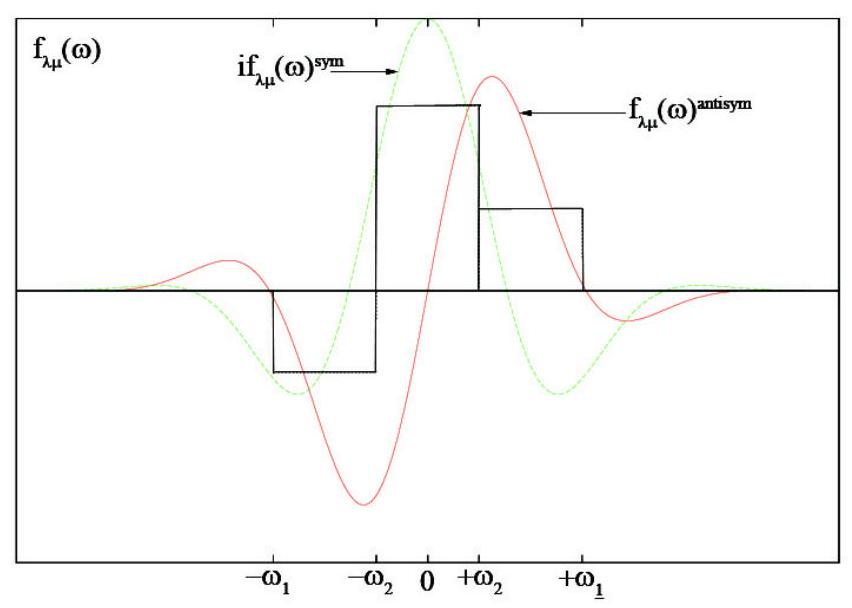
\includegraphics[max width=\textwidth]{2025_02_07_204a351db2d7f48b61ebg-074}
\end{center}

Figure 6.1: Actual and approximate Coulomb interaction strength functions. The fast approximation assumes that the antisymmetric component dominates in the ranges $-\omega_{1} \rightarrow-\omega_{2}$ and $+\omega_{2} \rightarrow+\omega_{1}$ while the symmetric component dominates in the range $-\omega_{2} \rightarrow+\omega_{2}$.\\
where $n, k$ are the spin plus parity of the initial and final states respectively. The transition multipolarity is $\lambda$.

For both $m=0$ and $m= \pm 1$ the function $f_{l m}(\omega)$ can be expressed as a sum of two components, one antisymmetric in $\omega$ and real, the other symmetric in $\omega$ and imaginary:


\begin{align*}
f_{l m}(\omega) & =f_{l m}(\omega)^{\text {antisym }}+i f_{l m}(\omega)^{\text {symm }}  \tag{6.12}\\
i f_{l m}(\omega)^{\text {symm }} & =Q_{l m}(\omega) \cos \left[\xi_{k n}(\varepsilon \sinh \omega+\omega)\right] \\
f_{l m}(\omega)^{\text {antisym }} & =Q_{l m}(\omega) \sin \left[\xi_{k n}(\varepsilon \sinh \omega+\omega)\right]
\end{align*}


These properties of the $f(\omega)$ function assure the unitarity of the right hand side operator of equation 6.10. Significant simplifications of the Coulomb excitation formalism can be achieved by replacing the $\omega$ dependent functions by constant effective interaction strengths extended only over finite ranges of $\omega$. For the most important $\Delta m=0$ couplings $f_{l m}^{s}(\omega)$ is localized around $\omega=0$, while $f_{l m}^{a}(\omega)$ is negligible anywhere except in the vicinity of $\pm \omega_{0}, \omega_{0}$ being case-dependent. Following this observation, one can approximate the total interaction by assuming the effective, constant interaction strengths covering three regions completely separated in $\omega$; that is, an antisymmetric part, extended over a finite $\omega$ range around some value of $\omega=-\omega_{0}$, a symmetric part around $\omega=0$, and the reflection of the antisymmetric part around $\omega=\omega_{0}$, as schematically presented in Figure 6.1.

The $\Delta m= \pm 1$ couplings can be treated in a similar way, although the separation of symmetric and antisymmetric components in $\omega$ is not as pronounced in this case. Nevertheless, taking into account the weakness of these couplings and their second-order importance, it is not worthwhile to construct a more accurate approximation.

According to the above model, the system of differential equations describing the Coulomb excitation can be represented as three independent equations of the form:

\[
\begin{array}{lll}
\frac{d \bar{a}}{d \omega}=A_{1}^{*} \bar{a}(\omega) ; & \bar{a}_{o}=\bar{a}(-\infty) & \\
\frac{d \bar{a}}{d \omega}=\omega_{1} \leq \omega \leq-A_{2}^{*} \bar{a}(\omega) ; & \bar{a}_{o}=\bar{a}\left(-\omega_{2}\right) ; &  \tag{6.13}\\
-\omega_{2}<\omega \leq \omega_{2} \\
\frac{d \bar{a}}{d \omega}=-A_{1}^{*} \bar{a}(\omega) ; & \bar{a}_{o}=\bar{a}\left(\omega_{2}\right) ; & \\
\omega_{2}<\omega \leq \omega_{1}
\end{array}
\]

where the matrix operators $A^{*}$ result from replacing the functions $f_{l m}$ of equation 6.11 with effective constants over three specified ranges. The sequential set of equations 6.12 has an obvious solution:\\
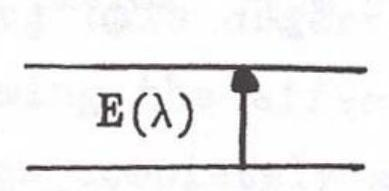
\includegraphics[max width=\textwidth, center]{2025_02_07_204a351db2d7f48b61ebg-075(1)}\\
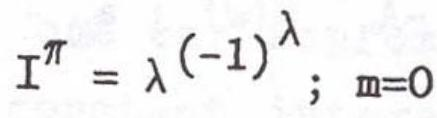
\includegraphics[max width=\textwidth, center]{2025_02_07_204a351db2d7f48b61ebg-075}

$$
I^{\pi}=0^{+}
$$

Figure 6.2: Two-level system


\begin{equation*}
\bar{a}(\infty)=\exp \left(-A_{1}\right) \exp \left(-A_{2}\right) \exp \left(A_{1}\right) \bar{a}(-\infty) \tag{6.14}
\end{equation*}


where the matrix operators $A$ correspond to $A^{*}$ in equation 6.13 , differing only by appropriate scaling to eliminate the independent variable ranges from the final formula. The $A$ matrices are purely real and fulfill the symmetry conditions:


\begin{align*}
A_{1 k i} & =-A_{1 i k}  \tag{6.15}\\
A_{2 k i} & =A_{2 i k}
\end{align*}


The relations 6.15 , resulting from the symmetry properties of the reduced matrix elements and coupling coefficients $\zeta$, assure the conservation of total excitation probability. The matrix elements of $A$ can be explicitly written as:


\begin{align*}
A_{l i k} & =M_{i k}^{(\lambda)} \cdot \zeta_{i k}^{(\lambda m)} \cdot q_{a}^{(\lambda m)}  \tag{6.16}\\
A_{2 i k} & =M_{i k}^{(\lambda)} \cdot \zeta_{i k}^{(\lambda m)} \cdot q_{s}^{(\lambda m)}
\end{align*}


where $q_{a}^{(\lambda m)}$ and $q_{s}^{(\lambda m)}$ are effective strength parameters, replacing $f_{\lambda m}^{(a)}(\omega)$ and $f_{\lambda m}^{(s)}(\omega)$, respectively. These parameters are functions of $\epsilon$ and $\xi$, thus for a given experiment one needs to determine them as functions of $\xi$ only, the eccentricity $\epsilon$ assumed constant.

The most flexible way of obtaining the $q$ parameters is to extract them from the exact excitation calculation for a two-level system. Let us consider the simple case shown in Figure 6.2 with the reduced matrix element $M$ connecting the two levels.

For this case, the $A$ matrices are explicitly given as:


\begin{align*}
& A_{1}=\left(\begin{array}{cc}
0 & -q_{a}^{(\lambda 0)} M \zeta \\
q_{a}^{(\lambda 0)} M \zeta & 0
\end{array}\right)  \tag{6.17}\\
& A_{2}=\left(\begin{array}{cc}
0 & -q_{s}^{(\lambda 0)} M \zeta \\
q_{s}^{(\lambda 0)} M \zeta & 0
\end{array}\right)
\end{align*}


and, according to 6.14 :


\begin{align*}
a\left(0^{+}\right) & =\cos \left(q_{s}^{(\lambda 0)} M \zeta\right)+i \sin \left(q_{s}^{(\lambda 0)} M \zeta\right) \cdot \sin \left(2 q_{a}^{(\lambda 0)} M \zeta\right)  \tag{6.18}\\
a\left(I^{\pi}\right) & =-i \sin \left(q_{s}^{(\lambda 0)} M \zeta\right) \cdot \cos \left(2 q_{a}^{(\lambda 0)} M \zeta\right)
\end{align*}


The above yields:


\begin{align*}
& q_{s}^{(\lambda 0)}=\frac{\operatorname{Arccos}\left(\operatorname{Re~a}\left(0^{+}\right)\right)}{M \zeta}  \tag{6.19}\\
& q_{a}^{(\lambda 0)}=-\operatorname{arctg}\left(\frac{\operatorname{Im} a\left(0^{+}\right)}{\operatorname{Im} a\left(I^{\pi}\right)}\right) / 2 M \zeta
\end{align*}


\begin{center}
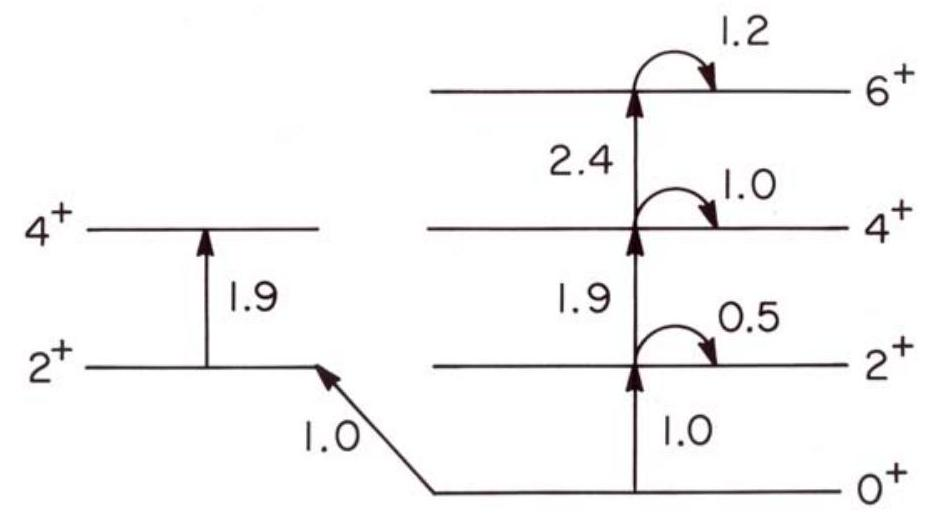
\includegraphics[max width=\textwidth]{2025_02_07_204a351db2d7f48b61ebg-076}
\end{center}

Figure 6.3: Model Coulomb excitation case for $200 \mathrm{MeV}{ }^{56} N i$ beam on $Z=46, A=110$ nucleus. The matrix elements quoted are in units of $e, b$.

Using equation 6.19 it is possible to extract $q$ parameters substituting the excitation amplitudes resulting from the exact calculation, i.e., the solution of equation 3.20. A similar procedure can be applied to find the $q$ parameters corresponding to $\Delta m= \pm 1$ coupling.

The appropriate formula, equation 6.14 , works best in cases where the range of $\xi$-parameters is not excessively wide. This practically assures good performance in all cases of multiple Coulomb excitation, since, as discussed in Chapter 3, small values of $\xi$ are required to produce significant multiple excitation. To demonstrate the reliability of the semi-analytic approximation, let us consider a test case in which we simulate the Coulomb excitation of a $Z=46, A=110$ nucleus by a $200 \mathrm{MeV}{ }^{58} N i$ beam. The target nucleus is described by the level and coupling scheme (of course having nothing to do with the real ${ }^{110} P d$ ) shown in Figure 6.3. The level energy differences all are assumed to be equal to 0.5 MeV . All reduced $E 2$ matrix elements are given in units of e.b.

Comparison between the exact solution of equation. 3.18 and the approximate solution using equation 6.14 is as follows:

Table 6.2: Excitation amplitude (population)

\begin{center}
\begin{tabular}{|c|c|c|}
\hline
Levels & Exact calculation; eq. 3.20 & Fast approximation: eq. 6.14 \\
\hline
$0^{+}$ & $.494+.018 \mathrm{i}(.244)$ & $.499-.145 \mathrm{i}(.265)$ \\
\hline
$2^{+}$ & $.134+.139 \mathrm{i}(.032)$ & $.161+.096 \mathrm{i}(.035)$ \\
\hline
$4^{+}$ & $-.205+.391 \mathrm{i}(.194)$ & $-.186+.407 \mathrm{i}(.200)$ \\
\hline
$6^{+}$ & $-.176+.388 \mathrm{i}(.145)$ & $-.192+.312 \mathrm{i}(.134)$ \\
\hline
$2^{+}$ & $.276+.266 \mathrm{i}(.119)$ & $.284+.157 \mathrm{i}(.105)$ \\
\hline
$4^{+}$ & $-.482-.165 \mathrm{i}(.260)$ & $-.445-.236 \mathrm{i}(.254)$ \\
\hline
\end{tabular}
\end{center}

The $A$ matrix approximation is generally more than adequate to calculate derivatives of level populations with respect to the matrix elements, using internal correction factors described earlier to account for differences between the approximate and the exact approach. It also provides a useful tool to investigate (at least qualitatively) the Coulomb excitation process.

As an example, let us consider the influence of the quadrupole moment for the two-level system shown in Figure 6.4 and discussed extensively in the Alder-Winther monograph [ALD75].

To simplify the notation, let us denote:\\
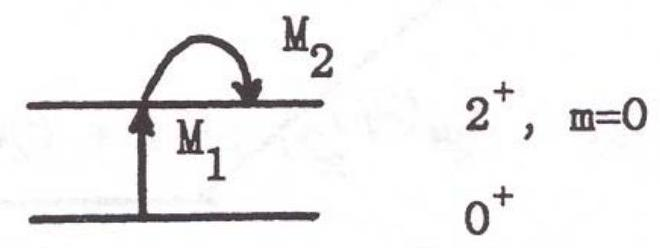
\includegraphics[max width=\textwidth, center]{2025_02_07_204a351db2d7f48b61ebg-077}

Figure 6.4: Reorientation effect for the two-level system.


\begin{align*}
& q_{s}^{(20)}\left(0^{+} \rightarrow 2^{+}\right) \cdot M_{1} \zeta_{0^{++2^{+}}}^{(20)}=q \\
& q_{a}^{(20)}\left(0^{+} \rightarrow 2^{+}\right) \cdot M_{1} \zeta_{0^{+} 2^{+}}^{(20)}=q_{1}  \tag{6.20}\\
& q_{s}^{(20)}\left(2^{+} \rightarrow 2^{+}\right) \cdot M_{2} \zeta_{2^{+2+} 2^{+}}^{(20)}=Q
\end{align*}


Note that there is no antisymmetric component of the interaction for the quadrupole moment, since $\zeta=0$.

The $A$ matrices can then be written as:


\begin{align*}
& A_{1}=\left(\begin{array}{cc}
0 & -q_{1} \\
q_{1} & 0
\end{array}\right)  \tag{6.21}\\
& A_{2}=\left(\begin{array}{cc}
0 & q \\
q & Q
\end{array}\right)
\end{align*}


yielding:


\begin{align*}
\exp \left( \pm A_{1}\right) & =\left(\begin{array}{cc}
\cos q_{1} & \mp \sin q_{1} \\
\pm \sin q_{1} & \cos q_{1}
\end{array}\right)  \tag{6.22}\\
\exp \left(-i A_{2}\right) & =e^{i Q / 2}\left(\begin{array}{cc}
\cos p-\frac{1}{2} i \frac{Q}{p} \sin p & -\frac{i q}{p} \sin p \\
-\frac{i q}{p} \sin p & \cos p+\frac{1}{2} i \frac{Q}{p} \sin p
\end{array}\right)
\end{align*}


where

$$
p=\frac{1}{2}\left(Q^{2}+4 q^{2}\right)^{1 / 2}
$$

Using 6.14 gives:


\begin{equation*}
a_{2^{+}}=\frac{1}{2} i e^{i Q / 2} \frac{\sin p}{p}\left(Q \sin 2 q_{1}-2 q \cos 2 q_{1}\right) \tag{6.23}
\end{equation*}


which results in an excitation probability:


\begin{equation*}
P_{2+}=\frac{1}{4} \frac{\sin ^{2} p}{p^{2}}\left(Q \sin 2 q_{1}-2 q \cos 2 q_{1}\right)^{2} \tag{6.24}
\end{equation*}


The formula 6.24 is a generalization of the second-order perturbation theory result. Taking into account only the lowest order terms in $q, q_{1}$, and $Q$ gives:


\begin{equation*}
P_{2+} \approx q^{2}\left(1-Q \cdot \frac{q_{1}}{q}\right)^{2} \tag{6.25}
\end{equation*}


as predicted by second-order perturbation theory. It should be observed, that the influence of the quadrupole moment is significant only if the ratio of antisymmetric to symmetric $q$ parameters is high, which physically corresponds to a large value of $\xi$. As can be seen from 6.23 , the primary effect of the static moment is rotation\\
of the complex excitation amplitude, due to the $\exp (i Q / 2)$ factor. This allows rather accurate measurements of static moments in cases of interfering paths of excitation, i.e., when a state is excited in a comparable way via two or more sequences of couplings. In this situation the phases that the partial excitation amplitudes are summed are of primary importance.

In general, 6.19 is only a semianalytical formula, since for complex cases, exponents of the $A$ matrices must be evaluated numerically. Nevertheless, numerical determination of $\exp (A)$ operators is much faster than the integration of a system of differential equations. It is worth observing that the truncation of the Taylor series approximating the $\exp (A)$ operators provides a way to generate perturbation theory of a given order, thus being useful for investigating weak excitation processes.

The above fast-matrix approximation is used in GOSIA to evaluate the Coulomb excitation amplitudes within the minimization and error estimation modules. The level and matrix element scheme used for this procedure is identical to that employed for the full calculation with two exceptions. First, the number of magnetic substates taken into account beyond the main excitation path, $n$, can only assume values of 0 or 1. Second, only $E 1$ through $E 6$ multipolarities are used to construct the matrix approximation. The only additional information needed is the knowledge of the effective strength parameters, $q_{a}$ and $q_{s}$, as introduced in the formula 6.16. The effective strength parameters depend on the experimental conditions as well as on the energy difference of the levels coupled by a given matrix element, and thus, in principle, should be assigned to every matrix element independently for each experiment. However, from a point of view of the memory requirements, this approach is not feasible, therefore it has been chosen to create the maps of $q$ parameters at discrete $\xi$ points for every experiment and to obtain the actual parameters using linear interpolation. The $q$ parameters should be independent of the coupling strength $\zeta$ (Equation 3.23) if the model was perfect, but practically some weak $\zeta$ dependence is still present. A significant improvement of the matrix approximation accuracy can thus be obtained by including the first-order $\zeta$-dependence correction for the prevailing $\Delta m=0$ couplings, which is equivalent to defining the $q$-parameters as:


\begin{equation*}
q(\Delta m=0 ; \xi, \zeta)=a(\xi) M \zeta+b(\xi) \tag{6.26}
\end{equation*}


where $M$ symbolically stands for a matrix element associated with a given coupling. The $q$ parameters for $\Delta m= \pm 1$ couplings are still treated as functions of $\xi$ only, the possible improvement of the approximation introduced by the $\zeta$-dependent correction being negligible because of the weakness of these couplings.

The map of the $q$ parameters is generated and stored when a separate option (chapter 7.15) is executed and read if either the minimization command (chapter 7.18) or the error estimation command (chapter 7.6) is encountered. For each experiment, GOSIA establishes the ranges of $\xi$ and $\zeta$ according to the level scheme (the maximum decay energy defines the maximum value of $\xi$ ) and the specified limits of the matrix elements (chapters $7.16,7.17$ ) which determine the maximum value of $\zeta$. The $q$ parameters are extracted following the method discussed in chapter 6.2 using the two-level system described using preset values of $\zeta$ and $\xi$. For each $\xi$ meshpoint, fifty values of $\zeta$, covering the whole range, are used to fit the coefficients $a$ and $b$ (equation 6.26 ) by the usual linear regression ( $\Delta m=0$ only ). Ten $\xi$ meshpoints are used for all multipolarities, thus the map consists of ten pairs $(a, b)$ for each multipolarity and experiment for both $q_{a}$ and $q_{s}$ corresponding to $\Delta m=0$ couplings while the $\Delta m= \pm 1$ are treated as $\zeta$-independent, therefore only the $a$ and $b$ coefficients are computed and stored.

The $q$ parameters map, once generated, need not be recalculated by the user unless the ranges of $\xi$ or $\zeta$ were changed by including additional levels or couplings resulting in a higher maximum decay energy or by expanding the limits of the matrix elements. It is always recommended to keep these ranges at a reasonable minimum, especially the range of $\xi$. This can be achieved by eliminating couplings between levels having no influence on both excitation and deexcitation, but creating high-energy decays. As a rule, the matrix approximation reliability improves with decreasing values of $\xi$, thus by narrowing its range one usually obtains faster convergence of the minimization. Calculation of the map is much faster, $\sim 1 s$, than other calculations required to fit matrix elements.

The approximate excitation amplitudes are computed according to equation 6.14 , with $A$ matrices defined by 6.16 . An algorithm:


\begin{align*}
{\overline{a_{p}}}^{(0)} & =\bar{a}^{(0)}  \tag{6.27}\\
{\overline{a_{p}}}^{(n+1)} & =\overline{1}_{n+1} A{\overline{a_{p}}}^{(n)} \\
\bar{a}^{(n+1)} & =\bar{a}^{(n)}+{\overline{a_{p}}}^{(n+1)}
\end{align*}


equivalent to the Taylor series expansion, is used to evaluate iteratively the product of the matrix exponentials acting on the initial amplitude vector $\bar{a}=\bar{a}(\omega=-\infty)$. The convergence of this procedure is controlled by monitoring the sum of excitation probabilities and the evaluation of matrix exponentials is truncated if this sum differs from unity by less than user-specified accuracy, see chapter 7.18. In some cases, the summation 6.27 may not converge within the requested accuracy due to the computer-dependent roundoff error propagation. This usually happens when the matrix elements of the $A$ operators are large. To overcome this problem it may be necessary to logically subdivide the matrix operators using the identity:


\begin{equation*}
\exp (A) \bar{a}=\exp \left(\frac{A}{2}\right) \exp \left(\frac{A}{2}\right) \bar{a} \tag{6.28}
\end{equation*}


which is done by GOSIA automatically, with the message:

\section*{EXP(A) EXPANSION FAILURE- EXP. N NEW SUBDIVISION(L,K)}
issued, specifying experiment number $N$ and number of times $K$ the subdivision of either $A_{1}$ or $A_{2}$ operator ( $L=1$ or 2 ) was performed. Usually a single subdivision is sufficient to assure the default accuracy $10^{-5}$ for any Coulomb excitation experiment, thus more subdivisions probably points to unreasonable values of the matrix elements. Inclusion of data for which the required matrix elements are undefined can lead to an endless loop with the expansion failure reported at each iteration, and the job must be terminated by the user.

The matrix operators used for the fast approximation are sparse and are never stored as matrices. Instead, the expansion 6.27 is performed using the fact that non-zero elements of these operators correspond to the matrix elements as follows from 6.16, therefore the catalog of the matrix elements is used to avoid dummy multiplications. The resulting excitation amplitudes then are used to calculate the statistical tensors exactly like the solution of the full Coulomb excitation coupled channel calculation.

\subsection*{6.3 Adiabaticity limitations}
Recent advances in detector technology have resulted in a tremendous increase in detection sensitivity that has led to the need for Coulomb excitation calculations that challenge the adiabaticity limitations built into the current version of GOSIA in 1980 [CLI08]. The adiabaticity can be expressed to first order by


\begin{equation*}
\xi_{k n} \sim \frac{Z_{1} Z_{2} A_{1}^{\frac{1}{2}}}{12.65} \frac{\left(E_{n-} E_{k}\right)}{E_{p} \sqrt{E_{p}}} \tag{3.35}
\end{equation*}


The orbit eccentricity $\epsilon$, is expressed in terms of the center-of-mass scattering angle $\theta_{c m}$ :


\begin{equation*}
\epsilon=\frac{1}{\sin \frac{\theta_{c m}}{2}} \tag{3.11}
\end{equation*}


Figure 6.5 shows that the ratio of the adiabaticity to transition energy is roughly constant at $\frac{\xi_{k n}}{\Delta E_{n k}} \approx 0.5$ for safe bombarding energies. This ratio is higher using lower bombarding energies but this is compensated by the fact that the higher $\Delta E_{n k}$ transitions are not appreciably excited. Recent Coulomb excitation studies can involve excitation energies as large as 4.4 MeV for light nuclei like ${ }^{12} \mathrm{C}, 3.8 \mathrm{MeV}$ in ${ }^{48} \mathrm{Ca}$, and 2.6 MeV in ${ }^{208} \mathrm{~Pb}$. These imply that the required range is $\xi_{k n} \leq 2.2$. For backscattering $\epsilon=1$ the $E 2$ orbital integral $R_{2 \mu}(\epsilon, \xi)$ drops to $7.3 \times 10^{-3}$ for $\xi_{k n}=2$; in addition the $\gamma$-ray detection efficiencies drop rapidly at the corresponding $\gamma$-ray energy of $\approx 4 \mathrm{MeV}$. As a consequence, excitation probabilities at $\xi_{k n} \approx 2.2$ correspond to the upper limit of experimental sensitivity available today and the practical upper bound to use in Gosia is $\xi_{k n}<2.5$.

The eccentricity $\epsilon$ increases rapidly when $\theta_{c m}$ is small, e.g., values are $\epsilon=5$ at $\theta_{c m}=23^{\circ}$ and $\epsilon=10$ at $\theta_{c m}=11.5^{\circ}$. Typical Coulomb excitation experiments involve detection of scattered ions between $20^{\circ} \leq$ $\theta_{L a b} \leq 180^{\circ}$ which implies eccentricity values in the range $1.0 \leq \epsilon \leq 5$. However, for small adiabaticity $\xi$, users may need to integrate to more forward angles to where the cross section is negligible, that is, to about an eccentricity of $\epsilon=10$. Thus it is reasonable to assume a maximum range of $1.0 \leq \epsilon \leq 10$.

The excitation probability for Coulomb excitation depends sensitively on the "adiabaticity product" $\xi_{k n} \epsilon$.Inspection of the orbital integrals dependence of $\epsilon$ and $\xi$ (see Alder and Winther, Rev. Mod. Phys. 28\\
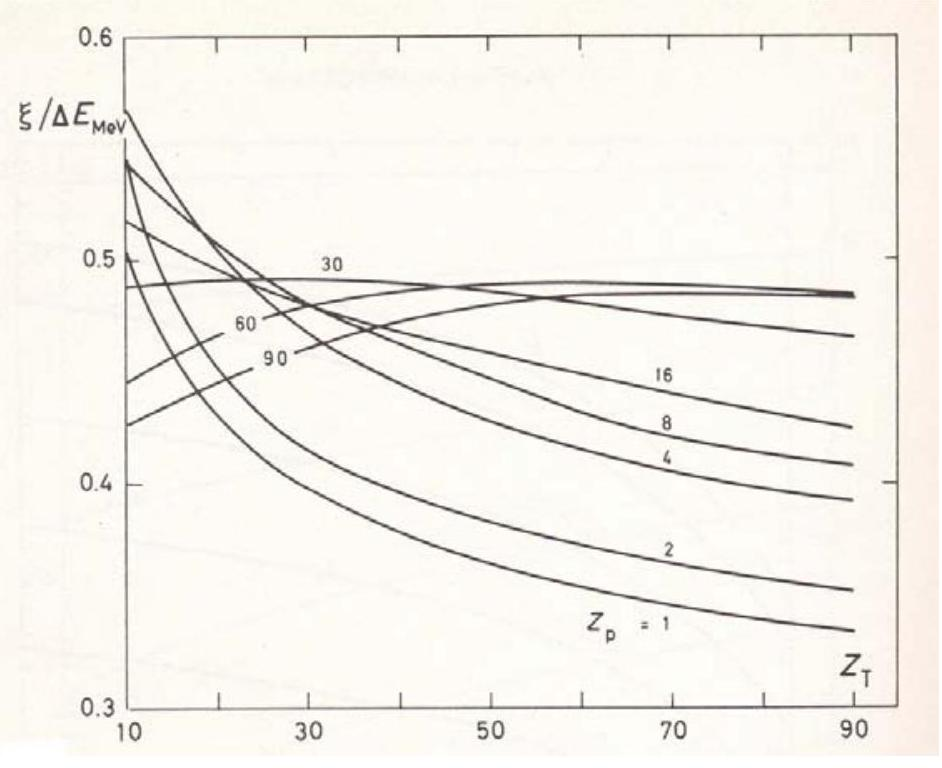
\includegraphics[max width=\textwidth, center]{2025_02_07_204a351db2d7f48b61ebg-080}

Figure 6.5: The ratio $\xi_{N M} / \Delta E_{N M}$ versus $Z_{T}$ and $Z_{P}$ for Coulomb excitation at the maximum safe bombarding energy. Taken from [ALD75]\\
(1956) 478) was used to select a practical range of the adiabaticity product for Gosia. The maximum values of the classical orbital integrals for E2excitation are $\leq 10^{-6}$ when the product $\xi_{k n} \epsilon=10$ and are $\leq 10^{-5}$ when $\xi_{k n} \epsilon=7.5$. These suggest that the upper bound for practical experiments should be $\xi_{k n} \epsilon \leq 10$ but most experiments will typically involve values of this product of $\xi_{k n} \epsilon \leq 5$.

The system of coupled differential equations for the excitation amplitudes $a_{k}$ is given by equation 3.20


\begin{equation*}
\frac{d a_{k}}{d \omega}=-i \sum_{\lambda \mu n} Q_{\lambda \mu}(\epsilon, \omega) \zeta_{k n}^{(\lambda \mu)} \cdot<I_{k}\|M(\lambda)\| I_{n}>\cdot \exp \left(i \xi_{k n}(\epsilon \sinh \omega+\omega)\right) \cdot a_{n}(\omega) \tag{3.20}
\end{equation*}


The most time-consuming aspect of solving the coupled equations using Gosia involves numerically evaluating the orbital integrals $R_{\lambda \mu}(\epsilon, \xi)$ for each channel where


\begin{equation*}
R_{\lambda \mu}(\epsilon, \xi)=\int_{-\infty}^{\infty} Q_{\lambda \mu}(\epsilon, \omega) \exp (i \xi(\epsilon \sinh \omega+\omega)) d \omega \tag{6.29}
\end{equation*}


Currently Gosia stores the $Q_{\lambda \mu}(\epsilon, \omega)$ collision functions with a spacing of $\Delta \omega=0.03$. To speed up the integration, GOSIA incorporates an accuracy test that can integrate using multiples of the minimum step size depending on the accuracy test. The errors that are encountered during evaluation of the orbital integration of the coupled differential equations are not associated with the accuracy of the $Q_{\lambda \mu}(\epsilon, \omega)$ collision functions. Rather they are due to the high rotation frequency of the exponential $e^{i \phi}$ phase-factor term that occurs at large $|\omega|$. This phase $\phi$ has the following dependence on $\omega$


\begin{equation*}
\phi=\xi_{k n} \epsilon \sinh \omega+\xi_{k n} \omega \tag{6.30}
\end{equation*}


This phase increases exponentially with $\omega$ at large values of $|\omega|$ and the highest oscillation frequency occurs at the largest magnitude of $\omega=\left|\omega_{\max }\right|$.

The rotational frequency of the phase is given by


\begin{equation*}
\nu=\frac{1}{2 \pi} \frac{d \phi}{d \omega}=\frac{\xi_{k n} \epsilon \cosh \omega+\xi_{k n}}{2 \pi} \tag{6.31}
\end{equation*}


At large $|\omega|$, where $\epsilon \cosh \omega \gg 1$, the rate of change in phase is approximately proportional to the product $\xi_{k n} \epsilon \cosh \omega$. The oscillation frequency depends strongly on the adiabaticity product $\xi_{k n} \epsilon$ which is largest for\\
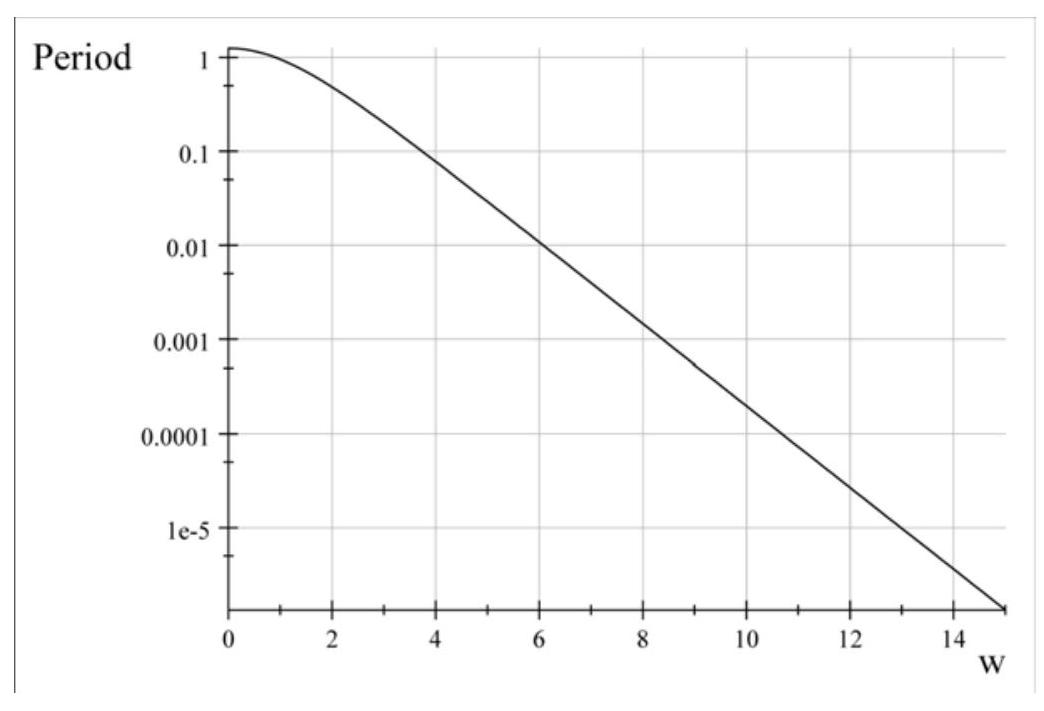
\includegraphics[max width=\textwidth, center]{2025_02_07_204a351db2d7f48b61ebg-081}

Figure 6.6: The period for one cycle of rotation of the phase factor and a function of $\omega$ for the case of 300 $\mathrm{MeV}{ }^{136} \mathrm{Xe}$ scattered at $\theta_{c m}=95^{\circ}$ exciting a $3 \mathrm{MeV} 2^{+}$state in ${ }^{180} \mathrm{~W}$. This case corresponds to $\xi=2.13$, and $\epsilon=1.356$ giving the product $\xi \epsilon=2.88$.\\
large transition energies, where $\xi_{k n}$ is large, as well as at forward angles, where $\epsilon \equiv \frac{1}{\sin \frac{\theta_{c m}}{2}}$ is large. The $\cosh \omega$ dependence implies that the oscillation frequency increases rapidly with increase in $|\omega|$.

Evaluation of the orbit integration of the coupled equations using the current version of Gosia is not limited by the accuracy of the collision functions $Q_{\lambda \mu}(\epsilon, \omega)$. The limit to the accuracy of the integration is set by the rotation period of the phase factor $\phi=\xi_{k n}(\epsilon \sinh \omega+\omega)$ which becomes comparable to, or less than, the integration step size $\Delta \omega$ at large $|\omega|$ which can result in erratic, unreliable, and wrong results and the error usually is not visible to the user. For example the current version of Gosia produces reliable and accurate results for $E 2$ excitation if the product of the adiabaticity and eccentricity $\xi \epsilon \leq 1.0$, while the upper limit for $E 1$ is $\xi \epsilon \leq 0.008$ which is far below typical values encountered in $E 1$ Coulomb excitation. Moreover, the accuracy parameter, which controls both the step size and range of integration, can exacerbate the above problem by extending the range of integration into a region where the code fails at even lower adiabaticity and also where the code points outside of array boundaries.

The period $\tau$ for one cycle of rotation of the phase is given by the reciprocal of the rotational frequency


\begin{equation*}
\tau=\frac{2 \pi}{\xi_{k n} \epsilon \cosh \omega+\xi_{k n}} \tag{6.32}
\end{equation*}


Note that the period for rotation of the phase is independent of multipole order $\lambda$. Figure 6.6 shows an example of the dependence of the phase rotation period $\tau$ on $\omega$ for the case of a $300 \mathrm{MeV}{ }^{136} \mathrm{Xe}$ beam scattered at $\theta_{c m}=95^{\circ}$ exciting a hypothetical $3 \mathrm{MeV} 2^{+}$state in a ${ }^{180} \mathrm{~W}$ target. This corresponds to $\xi=2.13$, and $\epsilon=1.356$ giving the adiabaticity product to be $\xi \epsilon=2.88$.

A Gosia simulation of the time dependence of the excitation probability along the semiclassical orbit for the above case is shown in Figure 6.7. The excitation probability for the incoming trajectory exhibits a staircase behaviour at large $|\omega|$, which for small $|\omega|$, develops into an oscillation extending in to $|\omega| \approx-3$. The mirror behaviour occurs on the exit trajectory except it is as not as visible due to the offset by the residual final excitation probability. The impact on the exit part of the trajectory is clearly visible even on the logarithmic plot meaning that the impact on the final probability is significant. This pathological behaviour is more pronounced for $E 1$ excitation where $\omega_{\max }=10.8$ at which the oscillation period is orders of magnitude smaller than the step size as shown in Figure 6.6.

Gosia has a minimum step size $\Delta \omega=0.03$ which, as shown in Figure 6.6, equals the oscillation period at about $|\omega|=5$ where the amplitude in figure 6.7 exhibits a sharp spike downward. The plateau extends inwards to where the oscillation period is about four times the step size.

It is obvious from Figure 6.7 that the Gosia results are unreliable when the rotation period approaches\\
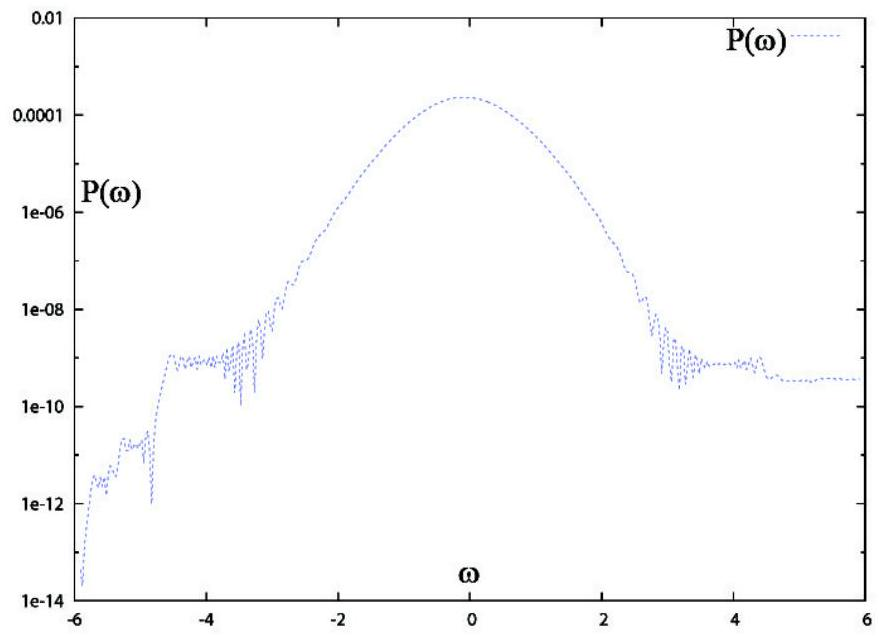
\includegraphics[max width=\textwidth, center]{2025_02_07_204a351db2d7f48b61ebg-082}

Figure 6.7: The time dependence of the excitation probability along the semiclassical trajectory for the case of $300 \mathrm{MeV}{ }^{136} \mathrm{Xe}$ scattered at $\theta_{c m}=95^{\circ}$ exciting a $3 \mathrm{MeV} 2^{+}$state in ${ }^{180} \mathrm{~W}$. This case corresponds to $\xi=2.13$, and $\epsilon=1.356$ giving the product $\xi \epsilon=2.88$.\\
the step size leading to a beat phenomenon between the step size and phase rotational period. It appears that at least 4 steps are needed per rotation cycle for reliable results and that pathological behaviour can be expected when the steps size is at a close multiple of the rotation frequency. Fortunately the product $Q_{\lambda \mu}(\epsilon, \omega) \zeta_{k n}^{(\lambda \mu)} .<I_{k}\|M(\lambda)\| I_{n}>$, which multiplies the exponential phase factor in the orbital integral, becomes very small as $\omega \rightarrow \omega_{\max }$ reducing the influence at the largest $|\omega|$. Thus the impact of the pathological behaviour in the phase factor term near $\omega_{\max }$ is decreased but there can still remain errors in the calculation for the asymptotic region as illustrated above. The worst pathological behaviour can be reduced by requiring that there be at least one sample per period at $\omega_{\max }$ since this implies that there will be 4 samples per period of oscillation in the regions where $Q_{\lambda \mu}(\epsilon, \omega) \zeta_{k n}^{(\lambda \mu)} \cdot<I_{k}\|M(\lambda)\| I_{n}>$ becomes significant. This extreme optimistic assumption implies that the upper limit on sampling period necessary to eliminate pathological behaviour is


\begin{equation*}
\nu=\frac{\xi_{k n} \epsilon \cosh \omega_{\max }+\xi_{k n}}{2 \pi} \leq \frac{1}{\Delta \omega} \tag{6.33}
\end{equation*}


which gives an upper limit of the adiabaticity product $\xi_{k n} \epsilon$


\begin{equation*}
\xi_{k n} \epsilon \leq \frac{2 \pi}{\Delta \omega \cosh \omega_{\max }} \tag{6.34}
\end{equation*}


Equation 6.34 can be used to estimate the most optimistic upper bound of $\xi_{k n} \epsilon$ that is required to minimize pathological behaviour during integration of the coupled differential equations for different step sizes. These optimistic upper bounds for $\xi_{k n} \epsilon$ are given in table 6.3 , while the numbers in brackets are the corresponding number of steps $N$ required for integration between the limits $-\omega_{\max }$ and $+\omega_{\max }$ assuming a constant value of $\Delta \omega$. Note that accurate integration requires lower upper limits than given in this table. It appears that for $E 2$ excitation the step size has to be reduced to $\Delta \omega=0.003$, that is, by more than an order of magnitude from the current minimum of $\Delta \omega=0.03$, to allow for accurate calculations up to adiabaticity values of $\xi_{k n} \epsilon \leq 10$. For $E 1$ excitation the step size needs to be reduced by three orders of magnitude!

Upper bounds for $\xi_{k n} \epsilon$ for different step sizes, $\Delta \omega$. (N) is the number of steps between $-\omega_{\text {max }}$ and $+\omega_{\text {max }}$

\begin{center}
\begin{tabular}{lcccc}
$E \lambda$ & $\omega_{\max }$ for $a_{c}=10^{-5}$ & $\xi_{k n} \epsilon(N)$ at $\Delta \omega=0.03$ & $\xi_{k n} \epsilon(N)$ at $\Delta \omega=0.01$ & $\xi_{k n} \epsilon(N)$ at $\Delta \omega=0.003$ \\
E1 & 10.82 & $0.0083(721)$ & $0.0251(1082)$ & $0.0837(7210)$ \\
E2 & 5.96 & $1.080(398)$ & $3.241(1192)$ & $10.804(3980)$ \\
E3 & 4.37 & $5.297(291)$ & $15.90(874)$ & $52.97(2910)$ \\
E4 & 3.59 & $11.55(240)$ & $34.65(718)$ & $115.5(2400)$ \\
E5 & 3.13 & $18.27(208)$ & $54.83(626)$ & $182.7(2080)$ \\
E6 & 2.88 & $23.44(192)$ & $70.32(576)$ & $234.4(1920)$ \\
\end{tabular}
\end{center}

Requesting a higher accuracy such as $a_{c}=10^{-6}$ actually decreases the accuracy during integration and can cause pathological behaviour increasing $\omega_{\max }$ to a point where the rotational frequency greatly exceeds the sampling frequency. For example, for $E 2$ excitation using $a_{c}=10^{-6}$ in equation 6.3 implies $\left|\omega_{\max }\right|$ increases from 5.96 to 14.0 which increases the rotation frequency by a factor of 3103 . This problem is known by experienced Gosia users.

An example of Coulomb excitation of a light nucleus is $E 2$ excitation of an assumed $4 \mathrm{MeV} 2^{+}$state in ${ }^{10} \mathrm{Be}$ using 33 MeV projectile excitation by a ${ }^{206} \mathrm{~Pb}$ target for scattering at $\theta_{c m}=30^{\circ}$ which corresponds to $\xi_{k n} \epsilon=7.7$. Reducing the minimum step size to $\Delta \omega=0.003$ raises the adiabaticity limit from $\xi_{k n} \epsilon=1.08$ to $\xi_{k n} \epsilon=10.8$ which is sufficient. Thus for $E 2$ excitation it appears desirable to reduce the step size from $\Delta \omega=0.03$ down to at least $\Delta \omega=0.003$. The ten-fold decrease in step size implies a ten-fold increase in the number of steps and a concomitant increase in computer processing time; currently the orbit integration already accounts for about $90 \%$ of the processing time. Another example is $600 \mathrm{MeV}{ }^{120} \mathrm{Sn}$ Coulomb exciting ${ }^{208} \mathrm{~Pb}$; using a step size of $\Delta \omega=0.03$ which implies that the $E 2$ transition excitation energy in ${ }^{208} \mathrm{~Pb}$ must not exceed 2.16 MeV for back scattering, while the transition energy must not exceed 0.56 MeV for $\theta_{c m}=30^{\circ}$. The first excited state of ${ }^{208} \mathrm{~Pb}$ is at 2.63 MeV which is above these adiabaticity limits. These results imply that the optimum step size for multipoles $E \lambda \leq 2$ should not be larger than $\Delta \omega=0.003$. Increasing the number of steps is not a viable remedy due to the increase in computing time. The current upper bounds of $\xi_{k n} \epsilon$ for $E 1$ excitation are much too small for practical applications.

In summary, implementing a 10 -fold decrease in the step size for $E 2$ excitation, and a 1000 fold decrease for $E 1$ excitation, are not viable due to the concomitant large increase in computing time. This problem is endemic to all semiclassical Coulomb excitation codes and thus a general solution is required. One proposal [CLI08] uses numerical integration of the coupled equations for a smaller range of $\omega$ and employs the fact that first-order perturbation theory is applicable in the asymptotic region with large $|\omega|$. Interpolation of precalculated perturbation values of the orbit integrals in these asymptotic regions can be used. Another alternative is use of new mathematical methods being developed to handle integration over integrands having extreme oscillatory behaviour. Implementation of a new algorithm is on hold pending unravelling of the complicated and extensive overlaying of the current GOSIA code.

The above discussion paints a worst-case scenario in a problem that is focussed primarily on E1 excitation. Observation of $E 1$ Coulomb excitation is very rare because the residual nucleon-nucleon interaction focusses the bulk of the $E 1$ strength in the high-lying giant dipole resonance exhausting the $E 1$ strength in the low-lying region reached by sub-barrier Coulomb excitation. But it behoves the user to check for problems even for $E 2$ excitation at high values of $\xi_{k n} \epsilon$.

\subsection*{6.4 Calculation of $\gamma$-ray Yields}
The Coulomb excitation statistical tensors rotated into the coordinate frame, having the $z$-axis along the incoming beam direction and the $x$-axis in the scattering plane (Fig. 4.1), are the interface between the excitation and deexcitation modules of GOSIA. The deexcitation module, activated automatically if OP,YIEL is encountered in the input stream, first establishes the decay scheme, common for all the experiments defined. The $\gamma$-decays are ordered "chronologically", i.e. from the highest to the lowest to take into account the effect of feeding. This has nothing to do with the user-defined sequence of the observed $\gamma$ yields, which can be defined arbitrarily and will be assigned by the code to the proper decays on a basis of the initial and final state indices provided by the user in an experimental yields file (7.33). The initialization of the decay module involves the calculation of the $F_{k}\left(\lambda \lambda^{\prime} I_{f} I\right)$ coefficients for each decay (see Eq. 4.9), which are not dependent\\
on either the matrix elements or on the experimental conditions, and are stored to avoid recalculating them for each experiment as well as for each set of the matrix elements during the minimization. The same holds for the decay amplitudes, $\delta_{\lambda}$, divided by the appropriate matrix elements (see Eq. 4.7).

The calculation of the $\gamma$ yields from the statistical tensors, for different experiments and matrix element sets, involves first the calculation of the deorientation effect and the transformation of the Coulomb excitation statistical tensors to the angular distribution tensors, $R_{k \chi}$, including the feeding from above (4.15). The tensors $R_{k \chi}$ are calculated in the system of coordinates originating in the decaying nucleus, as defined by Fig. 3.1, thus one has to transform them to the laboratory-fixed system. As long as the distance traveled by the decaying nucleus is negligible, this transformation consists of the relativistic velocity correction, outlined in Section 4.5. It should be noted, that this transformation is time-consuming and it is not performed when calculating the gradients used during minimization; its effect is absorbed into internal correction coefficients (6.6.3). Finally, using the symmetry properties of the decay tensors and the spherical harmonics, the double differential cross sections for the $\gamma$ decay from a state $I$ to a state $I_{f}$ can be written in the purely real form as:


\begin{equation*}
\frac{d^{2} \sigma\left(I \rightarrow I_{f}\right)}{d \Omega_{p} d \Omega_{\gamma}}=\sigma_{R}\left(\theta_{p}\right) \sum_{\substack{k \\ \chi \geq 0}} R_{k \chi}\left(I, I_{f} ; \theta_{p}\right) P_{k \chi}\left(\theta_{\gamma}\right)\left(2 \cos \chi\left(\phi_{p}-\phi_{\gamma}\right)-\delta_{\chi 0}\right) \tag{6.35}
\end{equation*}


where $P_{k \chi}$ stands for the Legendre spherical function and $\delta_{\chi 0}$ is the Kronecker symbol. It should be noted that Eq. 6.35 is given in the laboratory system of coordinates, differing from the scattering plane oriented system by the definition of the $\phi$ angle. The $\phi$ angle in the laboratory-fixed system of coordinates is given by the difference between the particle $\phi$ angle and the $\gamma$-ray $\phi$ angle, therefore the user-defined frame of coordinates is only restricted to have an origin corresponding to the position of the target and the $z$-axis along the beam direction, with the $x$ and $y$ axes defined arbitralily. As long as all the angles are consistently given in the same frame of coordinates, then the definition of the angular distribution is unique.

The double-differential cross section, defined by 6.35 , describes the angular distribution of $\gamma$ rays assuming that the direction of observation is well-defined, i.e., that the detector used can be treated as a $100 \%$ efficient point detector. As discussed in chapter 4.6, the finite size of a $\gamma$ detector results in the attenuation of the angular distribution, which can be taken into account by introducing the attenuation coefficients, $Q_{k \chi}$, transforming the angular distribution tensors, $R_{k \chi}$, according to:


\begin{equation*}
R_{k \chi} \rightarrow R_{k \chi} Q_{k \chi} \tag{6.36}
\end{equation*}


The attenuation coefficients $Q_{k \chi}$ depend on the geometry of the $\gamma$ detector, the $\gamma$-ray energy, absorbers, and the materials used for the $\gamma$-ray detection. It is assumed that the decay $\gamma$-rays were detected using coaxial Germanium detectors, optionally equipped with a set of absorbers frequently used to attenuate unwanted X-rays and low energy $\gamma$ rays. Typically, such detectors are used to study discrete $\gamma$-ray spectroscopy. For simplicity it is assumed that the Ge detectors have a symmetry axis that is aligned with the $\gamma$-ray emitter. For cylindrical symmetry only the $\chi=0$ components of $Q_{k \chi}$ are non-zero. Section 4.6 demonstrates that most axially-symmetry shapes are well approximated by assuming cylindrical symmetry. Therefore GOSIA uses equation 4.50 to calculate the cylindrically-symmetric $Q_{k 0}$ factors, which are named $Q_{k}$, in GOSIA. The absorption coefficients data for Ge and most commonly used absorber materials - Al, $\mathrm{Fe}, \mathrm{Cu}, \mathrm{Cd} / \mathrm{Sn}, \mathrm{Ta}$ and Pb - are built into the code. The $Q_{k}$ attenuation factors are $\gamma$-energy dependent, thus, as a compromise between the extensive storage and the necessity of recalculating them during each step of minimization or error calculation, a two-parameter fit of the $\gamma$-energy dependence is performed in a separate step, and only the fitted parameters are stored on a permanent file read in by GOSIA prior to the first $\gamma$-decay calculation. The fitted formula, which describes well the $\gamma$-energy dependence, is taken to be:


\begin{equation*}
Q_{k}\left(E_{\gamma}\right)=\frac{C_{2} Q_{k}\left(E_{0}\right)+C_{1}\left(E_{\gamma}-E_{0}\right)^{2}}{C_{2}+\left(E_{\gamma}-E_{0}\right)^{2}} \tag{6.37}
\end{equation*}


where $E_{0}=50 \mathrm{keV}$ with no graded absorbers or with a specified combination of $\mathrm{Al}, \mathrm{C}$, and Fe , while $E_{0}=80$, 100 , or 150 keV if $\mathrm{Cd} / \mathrm{Sn}$, Ta , or Pb absorber layers are employed as absorbers, respectively. The shift in "zero" energy is intended to provide a smooth dependence above the highest absorption cutoff point. It is assumed that the $\gamma$ transitions of energies below the highest cutoff point are of no interest, therefore no attempt is made to fit this region. $Q_{k}\left(E_{0}\right)$ in 6.37 stands for the attenuation coefficient for the "zero"\\
energy calculated according to the prescription of 4.6., while $C_{1}$ and $C_{2}$ are fitted to reproduce the energy dependence obtained using this formalism.

To reproduce the experimentally observed $\gamma$-ray intensities for a given beam energy and scattering angle $\theta_{p}$ the double-differential cross sections, as defined by 6.35 including the $\gamma$-ray detector solid angle attenuation factors (6.37), should be integrated over the $\phi$ angle range defining the particle detector shape for this scattering angle (note that from a point of view of the Coulomb excitation, an independent experiment is defined only by the scattering angle and the bombarding energy for the same beam). Also, the solid angle factor, $\sin (\theta)$, where $\theta$ is the projectile or target laboratory scattering angle, dependent on which particle has been detected, should be taken into account. The $\gamma$-ray decay intensities, referred to as "point yields", are therefore defined in GOSIA as:


\begin{equation*}
Y\left(\left(I \rightarrow I_{f}\right), \theta_{p}, E\right)=\sin \left(\theta_{p}\right) \int_{\phi_{p}} \frac{d^{2} \sigma\left(I \rightarrow I_{f}\right)}{d \Omega_{\gamma} d \Omega_{p}} d \phi_{p} \tag{6.38}
\end{equation*}


where the integrand is given by equation 6.35 . The integration over the $\phi$ angle is trivial since the $\phi$ dependence is analytical, described only by a single cosine function, as seen from equation 6.35 . According to the input units requested by GOSIA (Section 7) the yields will be calculated in units of $\mathrm{mb} / \mathrm{srad} / \mathrm{rad}$ ( i.e. millibarns per steradian, of the $\gamma$-ray solid angle, per radian of the particle scattering angle ). This holds for the $\gamma$ yields calculated using OP,POIN (7.19). The reproduction of the experimentally observed yields should, however, involve the integration over the particle scattering angle including the beam energy loss in the target, thus the fully integrated yields, obtained using OP,INTI, have a different meaning, as described in Section 6.5.

So far the effect of the geometric displacement of the origin of the system of coordinates due to in-flight decay has been neglected, i.e., it is assumed that all observed decays originate at the center of a target, thus the relativistic velocity correction is the only one needed to transform the nucleus-centered system to the laboratory-fixed system. This approximation is adequate as long as the mean lifetimes of the decaying states are in the subnanosecond range. For the cases involving longer-lived states, GOSIA provides an optional first-order treatment to correct for the geometric displacement. To treat this effect rigorously, one has to take into account both the change of the angles of the $\gamma$ detectors, as seen by the decaying nucleus, and the change of the solid angles subtended by the detectors. For a given direction of the recoil the observed yield of the decay of a state having the decay constant $\lambda$ can be written as:


\begin{equation*}
Y=\lambda \int_{0}^{\infty} \exp (-\lambda t) \cdot S(t) Y(t) d t \tag{6.39}
\end{equation*}


where $S(t)$ denotes the time dependence of the solid angle factor, while $Y(t)$ stands for the time dependence of the "point" angular distribution. To the lowest order, the product $S(t) Y(t)$ is expressed as:


\begin{equation*}
S(t) Y(t) \approx Y(0)+p t \tag{6.40}
\end{equation*}


where $p$ stands for the time derivative of this product taken at $t=0$ (note that $S(0)=1$, thus $S(0) Y(0)=Y(0)$ ). Inserting 6.40 into 6.39 and using the displacement distance, $s$, as an independent variable instead of time we finally obtain for mean lifetime $\tau$ :


\begin{equation*}
Y=Y(0)+\tau p \tag{6.41}
\end{equation*}


where $p$ is calculated numerically using a second set of yields evaluated in a point shifted by $s$ in the recoil direction, i.e.:


\begin{equation*}
p=\frac{S(s) Y(s)-Y(0)}{s} \tag{6.42}
\end{equation*}


where $S(s)$, is calculated assuming that the the displacement is small compared to the distance to the detector, $r_{0}$;


\begin{equation*}
S(s)=\frac{r_{0}^{2}}{\left(\bar{r}_{0}-\bar{s}\right)^{2}} \tag{6.43}
\end{equation*}


The displacement correction requires the $\gamma$ yields to be calculated twice for each evaluation, thus should be requested only when necessary to avoid slowing down the execution. The user is responsible to check that the first-order correction is adequate.

\subsection*{6.5 Integration over scattering angle and the energy loss}
\subsection*{6.5.1 Correction of experimental $p-\gamma$-ray yields}
The $\gamma$-decay formalism presented in Section 6.4 has so far assumed that the projectile scattering angle, $\theta_{p}$, and the bombarding energy, $E^{L}$, are constant for a given experiment. An exact reproduction of the experimentally observed $\gamma$ yields requires the integration over a finite scattering angle range and over the range of bombarding energies resulting from the projectile energy loss in a target. Using the definition of the "point" yields (6.38) the integrated yields, $Y_{i}\left(I \rightarrow I_{f}\right)$, are given by:


\begin{equation*}
Y_{i}\left(I \rightarrow I_{f}\right)=\int_{E_{\min }}^{E_{\max }} d E \frac{1}{\left(\frac{d E}{d x}\right)} \int_{\theta_{p, \min }}^{\theta_{p, \max }} Y\left(I \rightarrow I_{f}\right) d \theta_{p} \tag{6.44}
\end{equation*}


Note that both the Rutherford cross section and the solid angle factor, $\sin \theta_{p}$, are already included in the definition of the "point" yields, as well as integration over the detected particle $\phi$ angle.

The electronic stopping powers, $d E / d x$, in units of $M e V /\left(\mathrm{mg} / \mathrm{cm}^{2}\right)$, are defined by a user-specified table assuming common energy meshpoints for all experiments. As shown in chapter 5.3 it is recommended that the Ziegler[ZIE08] code SRIM be used to generate the user-specified table of stopping powers for use by GOSIA. The actual values of the stopping powers are obtained using spline interpolation. The double integral is then evaluated numerically using the discrete Simpson method. GOSIA performs the integration in two separate steps - first, the full Coulomb excitation coupled-channel calculation is done at each of the user-specified $\left(\theta_{p}, E\right)$ meshpoints to evaluate the "point" $\gamma$-yields, next, the actual numerical integration is performed according to the user-defined stepsizes in both dimensions. The point yields at the $\left(\theta_{p}, E\right)$ points as required by the fixed subdivisions are evaluated from the meshpoint values by logarithmic scale interpolation using the cubic spline subroutines SPLINE and SPLINT [PRE92]. The $\theta_{p}-E$ mesh is limited to a maximum of $100 x 100$ points, while up to 100 steps in angle and 100 steps in energy can be defined for subdivisions in the integration. [Do not use Lagrangian interpolation since it usually diverges using more than 20 mesh points for either $\theta_{p}$ or $E$.] Subdivision of the calculated mesh improves the accuracy of integration, since spline interpolation provides the information of the order dependence on the number of meshpoints, while the Simpson method is a fixed second-order algorithm. In addition, in cases which require a complicated $\phi_{p}\left(\theta_{p}\right)$ dependence, such as when using unusual-shaped, large-area, recoil-ion detectors that have kinematic and mechanical constraints, the user may optionally choose to input this dependence at both the meshpoints and subdivision level. The interpolation is then performed between the values divided by $\phi_{p}$ ranges to assure continuity, then the user-given dependence is used to estimate the yields at the subdivision meshpoints. The calculation of yields at the meshpoints requires the full coupled-channel Coulomb excitation calculation which is time-consuming. Consequently, one should balance the number of meshpoints needed for accuracy with the calculational time.

The integrated yields are calculated in units of $\mathrm{mb} /$ sterad times the target thickness $\left(\mathrm{mg} / \mathrm{cm}^{2}\right)$, which for thick targets, could be assumed to be the projectile range in the target.

The integration module of GOSIA can be used in conjunction with the correction module, invoked by the OP,CORR command (7.4), used to transform the actual experimentally-observed yields to the ones to which the subsequent fit of the matrix elements will be made. This operation is done to avoid the timeconsuming integration while fitting the matrix elements and is treated as an external level of iteration. An effect of the finite scattering angle and bombarding energy ranges as compared to the point values of the yields is not strongly dependent on the matrix elements, thus the fit can be done to the point values and then the integration/correction procedure can be repeated and the fit refined until the convergence is achieved. Usually no more than two integration/correction steps are necessary to obtain the final solution, even in case of the experiments performed without the particle- $\gamma$ coincidences, covering the full particle solid angle.

The correction module of GOSIA uses both the integrated yields and the point yields calculated at the mean scattering angle and bombarding energy, as defined in the EXPT (7.8) input, to transform the actual experimental yields according to:


\begin{equation*}
Y_{\exp }^{c}\left(I \rightarrow I_{f}\right)=Y_{\exp }\left(I \rightarrow I_{f}\right) \frac{Y_{\text {point }}\left(I \rightarrow I_{f}\right)}{Y_{\text {int }}\left(I \rightarrow I_{f}\right)} \tag{6.45}
\end{equation*}


where the superscript "c" stands for the "corrected" value.

To offset the numerical factor resulting from the energy-loss integration the lower-most yield observed in a $\gamma$-detector labeled as $\# 1$ for the first experiment defined in the EXPT input is renormalized in such a way that the corrected and actually observed yield are equal. This can be done because the knowledge of the absolute cross-section is not required by GOSIA, therefore, no matter how the relative cross-sections for the various experiments are defined, there is always at least one arbitrary normalization factor for the whole set of experiments. This normalization factor is fitted by GOSIA together with the matrix elements, as discussed in the following section (6.6). The renormalization procedure results in the "corrected" yields being as close as possible to the original values if the same target has been used for the whole set of the experiments analyzed, thus the energy-loss factor in the integration procedure is similar for the whole set of the experiments. However, one should be aware of the fact, that the correction factors may differ significantly for different experiments, thus the corrected yields, normalized to a user-specified transition, always given in the GOSIA output, should be used to confirm that the result is reasonable rather than absolute values. A final intergation can be performed to check the best solution.

\subsection*{6.5.2 Inverse kinematics}
\section*{The problem:}
Recent projectile Coulomb excitation studies using low-intensity rare-ion beams have employed inverse kinematics with $\tau>5$ in conjunction with target thickness for which the recoiling ions lose an appreciable fraction of the recoil energy. This introduced technical problems during the integration that necessitated the upgrade of the integration routine OP,INTG to OP,INTI that was developed by Nigel Warr [WAR08].

These technical problems encountered in the analysis for Coulomb excitation of the 0.7753 MeV firstexcited state of a $193.6 \mathrm{MeV}{ }^{88} \mathrm{Kr}$ beam by a $2.1 \mathrm{mg} / \mathrm{cm}^{2}$ thick ${ }^{12} \mathrm{C}$ target are summarized in this section to illustrate the problem and the solution. The energy loss in the target is 103.3 MeV giving an exit energy of 90.3 MeV . Figure 5.2 shows the correlation of the angles of the scattered ${ }^{88} \mathrm{Kr}$ and the recoiling ${ }^{12} \mathrm{C}$. The scattered ${ }^{88} \mathrm{Kr}$ nuclei of the beam have a maximum angle of $7.532^{\circ}$ and thus only the recoiling ${ }^{12} \mathrm{C}$ nuclei were detected since the particle detector had a hole from 0 to $16.4^{\circ}$. Integration is required over energy limits of 90.3 to 193.6 MeV and the $\theta$ limits of the particle detector of $16.4^{\circ}$ to $53.0^{\circ}$.

Meshpoints for energy can be selected in a range a little bit wider than 90.3 to 193.6 MeV , say from 85 to 205 MeV in 15 MeV steps. Choice of the $\theta$ meshpoints is more complicated since the OP,INTG routine requires the projectile angle in the laboratory frame not the detected target angle. Figure 6.8 shows the same as Fig. 5.2 but for the energies 85 MeV and 205 MeV , corresponding to the extrema of the meshpoints and only within the range of $16.4^{\circ}$ to $53.0^{\circ}$ corresponding to the angular range of the particle detector. It is seen that for any detected target recoil angle in the laboratory frame, the corresponding projectile scattering angle depends on the beam energy. However, the integration is over this beam energy, so it has to be evaluated at several different energies!\\
The fact that the scattered projectile angle is double-valued at each recoil target angle is not a problem since the events lying on the lower solution, for which the projectile scattering angle is less than a degree, correspond to very low target recoil energies (only a few hundred keV) so they will not be detected. Thus it is necessary to consider only the upper solution ranging from a scattered projectile angle of $4.64^{\circ}$ at the inner edge of the particle detector to a maximum of $7.53^{\circ}$ about $2 / 3$ of the way across the particle detector and falling to $6.77^{\circ}$ at the outer edge for an energy of 85 MeV , with slightly higher values at 205 MeV .

For the original integration code OP,INTG, the kinematics flag IKIN in EXPT option is used to select one of the double-valued scattered projectile angles. Angles to the left of the maximum correspond to higher angles of the projectile scattering angle in the centre of mass frame which can be accessed only with IKIN = 0 , while angles to the right of the maximum correspond to lower angles of the projectile scattering angle in the centre of mass frame, which can be accessed only with $I K I N=1$. Thus it is not possible to integrate over the whole particle detector in a single integration, that is, it has to be broken up into two separate pieces. At 85 MeV , the integration is taken over target recoil angles of $16.4^{\circ}$ to about $40.24^{\circ}$ with $I K I N=0$ and from $40.24^{\circ}$ to $53^{\circ}$ with $I K I N=1$ and then the results are summed to get the whole integral. At 205 MeV , the maximum is not at $40.24^{\circ}$ but at $40.75^{\circ}$, so the angle for which the change from $I K I N=0$ to $I K I N=1$ occurs is different. This means that it is not possible to integrate between $40.24^{\circ}$ and $40.75^{\circ}$ at all since the OP,INTG option in GOSIA requires the scattered projectile angle, not the detected target\\
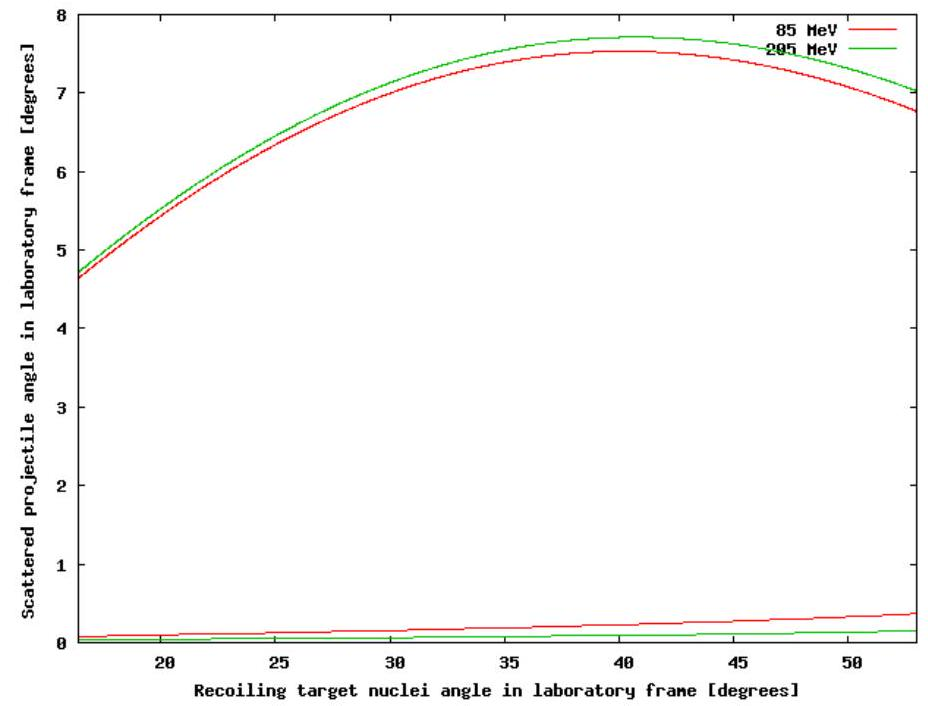
\includegraphics[max width=\textwidth, center]{2025_02_07_204a351db2d7f48b61ebg-088}

Figure 6.8: The angle of the scattered projectile in the laboratory frame for $194 \mathrm{MeV}{ }^{88} \mathrm{Kr}$ beam on a ${ }^{12} \mathrm{C}$ target. The scattering angle is two valued angle and is NOT well defined when recoiling target nuclei are detected.\\
recoil angles. So at 85 MeV , the $I K I N=0$ integration is over projectile scattering angles from $4.64^{\circ}$ to $7.53^{\circ}$ and with $I K I N=1$ from $6.77^{\circ}$ to $7.53^{\circ}$. However, for 205 MeV , the corresponding angles are $4.72^{\circ}$ to $7.71^{\circ}$ and from $7.03^{\circ}$ to $7.71^{\circ}$. Gosia automatically takes care of the calculation of these integration limits. However choosing a set of meshpoints is a problem since GOSIA can interpolate reliably but has problems with extrapolation; thus, meshpoints are needed which go beyond the limits required, or at very least up to them. But GOSIA only has one set of meshpoints, which has to work for all energies. For example, for meshpoints from $4.64^{\circ}$ to $7.71^{\circ}$ with $I K I N=0$ these points exactly span the region needed over the full range of energy. For 205 MeV , this is fine, since $4.64^{\circ}$ is lower than needed, but it is perfectly valid and $7.71^{\circ}$ is the maximum of the curve. However, for lower energies, this is no longer the case. For example, at 85 MeV , there is no solution to the calculation of the centre of mass angle, which gives a projectile scattering angle of $7.71^{\circ}$, since the maximum scattering angle is $7.53^{\circ}$. This means that the highest meshpoint that can be set is $7.53^{\circ}$, thus the meshpoints are from $4.64^{\circ}$ to $7.53^{\circ}$ i.e., exactly the range for the lowest energy meshpoint. Similarly for the case of $I K I N=1$, the meshpoint at $7.71^{\circ}$, but $7.53^{\circ}$ is used instead, thus the meshpoints range from $6.77^{\circ}$ to $7.53^{\circ}$. The result of these effects is that there are regions which are inaccessible to the calculation. At 205 MeV , there is a gap corresponding to target recoil angles of $34.7^{\circ}$ to $47.0^{\circ}$. At 85 MeV this effect is less dramatic as we only have the gap from $40.24^{\circ}$ to $40.75^{\circ}$ due to the change in the place where $I K I N$ flips over. This effect is illustrated in Fig. 6.9, where the red and green curves correspond to two energies with $I K I N=0$ and the blue and purple curves to the same energies with $I K I N=1$. The fact that the curves of a given energy do not meet shows that we have values of the recoiling target nuclei angle which cannot be accessed in the calculation. Moreover, since most of the cross section comes from the higher energies, this hole in the 205 MeV range is fatal.

One workaround is to perform the integration over the energy loss in the target manually, by dividing the target into virtual layers and performing the calculation for each layer with a single energy. This is particularly tedious as different limits and different meshpoints need to be set up for each energy. Extreme care has to be taken by the user, because using a limit which is too low results in missing cross-section and one which is too high results in Gosia aborting with an error.

One option considered was to changing everything over to the centre of mass system. Unfortunately this requires deep changes throughout Gosia which isvery complicated. Moreover, it does not solve the problem since the centre of mass angle, whether for the recoiling target or the scattered projectile nuclei, is undefined because the transformation from the laboratory frame of the detected particle to the centre of mass angle depends on the beam energy which is part of the integration. The only sensible unambigous frame, in\\
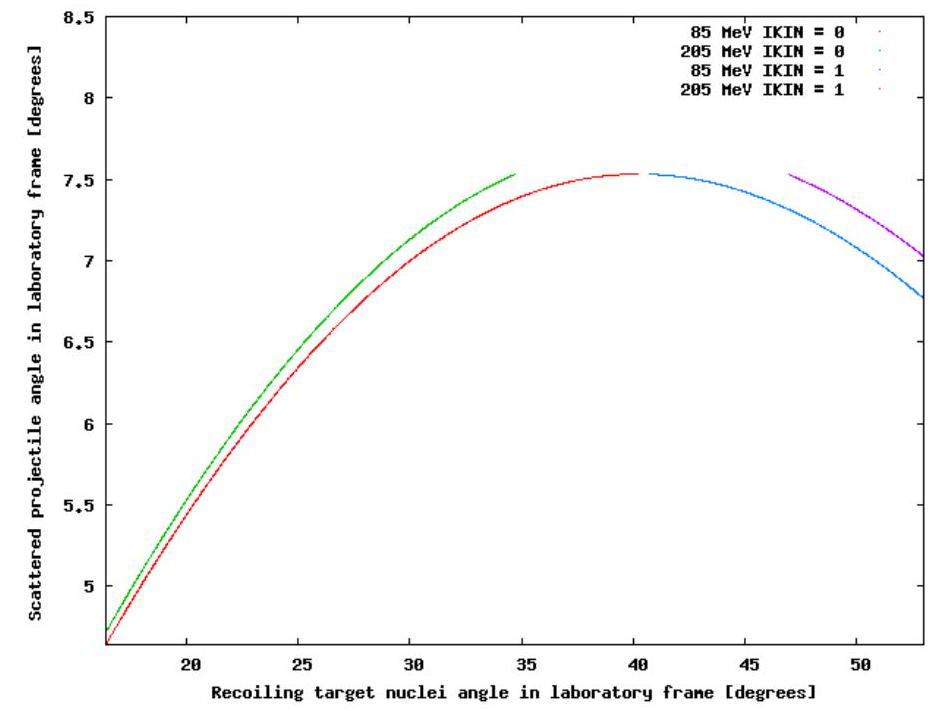
\includegraphics[max width=\textwidth, center]{2025_02_07_204a351db2d7f48b61ebg-089}

Figure 6.9: The angle of the scattered projectile in the laboratory frame for $194 \mathrm{MeV}{ }^{88} \mathrm{Kr}$ beam on a ${ }^{12} \mathrm{C}$ target for bombarding energies of 85 MeV and 205 MeV .\\
which to set limits, is in the laboratory frame of the detected recoil-ion. In this frame, the angles for which a scattered projectile can hit the particle detector do not depend on the energy of the beam. Similarly if the particle detector detects target recoils, we need to set the limits in the laboratory frame of the recoiling target nuclei.

Gosia requires the angular integration limits to be in the laboratory frame of the detected particle. However, the OP,INTG option in GOSIA does not follow this convention for the meshpoints. Instead it requires the meshpoints in the laboratory frame of the scattered projectile, regardless of which particle is detected. For the case where projectiles are detected, this is fine, of course, but when target nuclei are detected, it results in the problem of meshpoints that cannot be set correctly.

The conclusions derived from above discussion are:

\begin{itemize}
  \item The only frame of reference that should be used is the laboratory frame of the detected particles.
  \item OP,INTG does it correctly for the integration limits.
  \item OP,INTG does it correctly for the meshpoints, if the scattered projectiles are detected.
  \item OP,INTG is incorrect if the recoiling target nuclei are detected. This is the crux of the problem that OP,INTG is not useful for situations where the recoiling target nucleus is detected.
\end{itemize}

\section*{Solution to the problem}
The obvious solution is to give up the convention that the meshpoints are specified for the scattered projectile and instead use laboratory angles for the detected particle. This approach is used in the new integration routine, OP,INTI. The solution chosen is to convert the detected particle laboratory frame angles into the scattered projectile's laboratory frame for each energy and pass that value to the current version of Gosia, which would be unchanged. This has been implemented as a single new routine, called INVKIN, which is called inside both the energy and theta meshpoint loops. The problem corresponds to looking up the target recoil angle on Fig. 5.2 to find the corresponding scattered projectile angle. As can be seen, there are two solutions in general for each final energy. However, the lower value will generally correspond to target nuclei with too little energy to be detected. The following procedure is used in the subroutine INVKIN.

Let $\theta_{p_{C M}}$ be the angle of the scattered projectile in the centre of mass frame and $\theta_{p_{L a b}}$ be the equivalent in the laboratory frame, while $\theta_{t_{C M}}$ and $\theta_{t_{L a b}}$ are the equivalents for the target recoils.

We can write:


\begin{equation*}
\tan \theta_{p_{L a b}}=\frac{\sin \theta_{p_{C M}}}{\tau+\cos \theta_{p_{C M}}} \tag{6.46}
\end{equation*}


and


\begin{equation*}
\tan \theta_{t_{L a b}}=\frac{\sin \theta_{t_{C M}}}{\tau_{p}+\cos \theta_{t_{C M}}} \tag{6.47}
\end{equation*}


where


\begin{equation*}
\tau=\tau_{p} \frac{M_{p}}{M_{t}} \tag{6.48}
\end{equation*}


and


\begin{equation*}
\tau_{p}=\sqrt{\frac{E_{p}}{E_{p_{\min }}}} \tag{6.49}
\end{equation*}


where


\begin{equation*}
E_{p_{m i n}}=E_{p}-E_{x} \times a_{r e d} \tag{6.50}
\end{equation*}


and the reduced mass $a_{\text {red }}$ is given by


\begin{equation*}
a_{\text {red }}=1+\frac{M_{p}}{M_{t}} \tag{6.51}
\end{equation*}


and $E_{p}$ is the beam energy, $E_{x}$ is the energy of the excited state indicated by the parameter $N C M$ in suboption CONT, (by default the first excited state), and $M_{p}$ and $M_{t}$ are the projectile and target nuclei masses in AMU, respectively.

Since


\begin{equation*}
\theta_{p_{C M}}=\pi-\theta_{t_{C M}} \tag{6.52}
\end{equation*}


we can substitute in Eq. 6.47 and get


\begin{equation*}
\tan \theta_{t_{L a b}}=\frac{\sin \theta_{p_{C M}}}{\tau_{p}-\cos \theta_{p_{C M}}} \tag{6.53}
\end{equation*}


So the problem is one of inverting Eq. 6.53 to calculate $\theta_{p_{C M}}$ for a given $\theta_{t_{L a b}}$ and then substituting this value of $\theta_{p_{C M}}$ in Eq. 6.46 to obtain $\theta_{p_{L a b}}$, as required.

Let $x=\cos \theta_{p_{C M}}$ and $y=\tan \theta_{t_{L a b}}$. Then we have:


\begin{equation*}
y=\frac{\sqrt{1-x^{2}}}{\tau_{p}-x} \tag{6.54}
\end{equation*}


or


\begin{equation*}
y \tau_{p}-x y=\sqrt{1-x^{2}} \tag{6.55}
\end{equation*}


Squaring both sides we get a quadratic equation in $x$ :


\begin{equation*}
x^{2}\left(1+y^{2}\right)-2 \tau_{p} y^{2} x+\tau_{p}^{2} y^{2}-1=0 \tag{6.56}
\end{equation*}


Solving for $x$ we get:


\begin{equation*}
x=\frac{\tau_{p} y^{2} \pm \sqrt{\tau_{p}^{2} y^{4}-\left(1+y^{2}\right)\left(\tau_{p}^{2} y^{2}-1\right)}}{\left(1+y^{2}\right)} \tag{6.57}
\end{equation*}


Once we have $x=\cos \theta_{p_{C M}}$, we can substitute into Eq. 6.46.


\begin{equation*}
\theta_{p_{L a b}}=\arctan \frac{\sqrt{1-x^{2}}}{\tau+x} \tag{6.58}
\end{equation*}


This still requires knowing the correct value of IKIN which can be determined knowing the value of $\theta_{p_{C M}}$ for which $\theta_{p_{L a b}}$ has its maximum. Differentiating Eq. 6.46 and setting it to zero determines $\theta_{p_{C M}}$ which\\
can be substituted in Eq. 6.47 to get the corresponding value of $\theta_{t_{\text {Lab }}}$. This can be compared with the value being calculated which determines the value IKIN to be used in GOSIA.

So the problem is to evaluate:


\begin{equation*}
\frac{d}{d \theta_{p_{C M}}}\left(\arctan \left(\frac{\sin \theta_{p_{C M}}}{\tau+\cos \theta_{p_{C M}}}\right)\right)=0 \tag{6.59}
\end{equation*}


In fact, this can be acheived by evaluating:


\begin{equation*}
\frac{d}{d \theta_{p_{C M}}}\left(\frac{\sin \theta_{p_{C M}}}{\tau+\cos \theta_{p_{C M}}}\right)=0 \tag{6.60}
\end{equation*}


since the arc tangent only introduces a $1 /\left(1+x^{2}\right)$ term, which cannot be zero for real values of $\theta_{p_{C M}}$. Let $u=\sin \theta_{p_{C M}}$ and $v=\tau+\cos \theta_{p_{C M}}$.


\begin{equation*}
\frac{\left(\tau+\cos \theta_{p_{C M}}\right)\left(\frac{d}{\theta_{p_{C M}}}\left(\sin \theta_{p_{C M}}\right)\right)-\left(\sin \theta_{p_{C M}}\right)\left(\frac{d}{\theta_{p_{C M}}}\left(\tau+\cos \theta_{p_{C M}}\right)\right)}{\left(\tau+\cos \theta_{p_{C M}}\right)^{2}}=0 \tag{6.61}
\end{equation*}


or


\begin{gather*}
\left(\tau+\cos \theta_{p_{C M}}\right)\left(\cos \theta_{p_{C M}}\right)-\left(\sin \theta_{p_{C M}}\right)\left(-\sin \theta_{p_{C M}}\right)=0  \tag{6.62}\\
\tau \cos \theta_{p_{C M}}+\cos ^{2} \theta_{p_{C M}}+\sin ^{2} \theta_{p_{C M}}=0  \tag{6.63}\\
\cos \theta_{p_{C M}}=-\frac{1}{\tau} \tag{6.64}
\end{gather*}


This value of $\theta_{p_{C M}}$ can be substituted into Eq. 6.47 and if the required value of $\theta_{t_{L a b}}$ is greater than this value, then $I K I N=1$ is set internally by the code, otherwise it sets $I K I N=0$.

So far, the second solution corresponding to the minus sign in Eq. 6.57 has been neglected. It is clear that in the specific case of ${ }^{88} \mathrm{Kr}$ that we have considered here, this is not a problem. The lower solution, within the angle ranges of interest correspond to tiny target-recoil energies, that normally do not get out of the target or be detected by the particle detector. The Rutherford cross section for these nuclei is very large but the inelastic cross section typically negligible.

\section*{Implementation}
A new integration routine, called OP,INTI has been created that is identical to the OP,INTG code, except that the new INVKIN subroutine is invoked for inverse kinematics if the target nucleus angle is used, that is, the sign of $\theta_{L A B}$ is negative in suboption $E X P T$. The input format to GOSIA now requires the angles of the detected particle in the OP,INTI option rather than always using that of the scattered projectile. The OP,INTI routine was created in order to not break compatability with the old integration option OP,INTG which remains for running legacy inputs.

The OP,INTI option replaces the OP,INTG option and the laboratory angles of the detected particle are used for the meshpoints, rather than the laboratory angles for the scattered projectile. Note that for the case where the recoiling target nucleus is detected, at each beam energy and each angle during the integration, the subroutine INVKIN calculates the appropriate value of IKIN and sets this variable for GOSIA. This procedure allows the normal version of the GOSIA code to perform the correct integration for inverse kinematics with target nucleus detection. That is, this is included in the loop which calculates the $\theta$ and energy meshpoints, so it toggles IKIN as it goes over the angle where it should change, which is different for each energy value for a non-zero $Q$ value. Thus integration over the full angular range is automatically performed in a single calculation for target-recoil detection for inverse kinematics. This is essential for $\gamma$-ray yield data for a $\theta_{T}$ range that spans the maximum projectile scattering angle.

The following describes the behaviour of OP,INTI for the four cases with either projectile or target recoil detection and with either normal or inverse kinematics.

\begin{enumerate}
  \item Normal kinematics, either projectile or target detection; The kinematics are shown in figure $6.10 l e f t$. The red hatched region for recoil target detection usually can be ignored since the recoil energy is well below\\
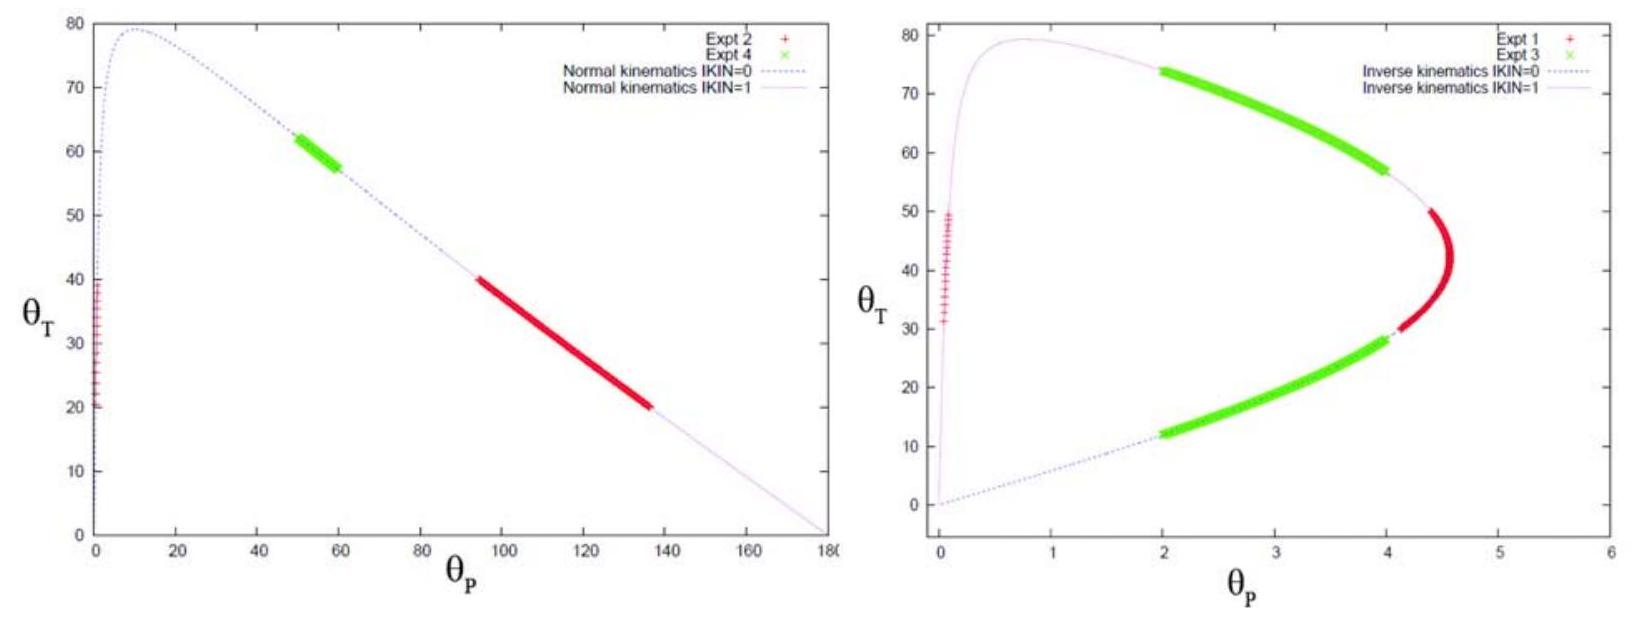
\includegraphics[max width=\textwidth, center]{2025_02_07_204a351db2d7f48b61ebg-092}
\end{enumerate}

Figure 6.10: Left; Normal kinematics: Target recoil angle $\theta_{T}$ versus projectile recoil angle $\theta_{P}$ in the laboratory frame for $64 \mathrm{MeV}{ }^{12} \mathrm{C}$ beam incident on a ${ }^{148} \mathrm{Sm}$ target. The red solid and hatched sections designate the two solutions for detection of the ${ }^{148} \mathrm{Sm}$ target recoils. The target recoil energies for the hatched solution are $<100 \mathrm{keV}$ which is below the recoil detector threshold. The solid green line designates detection of the ${ }^{12} \mathrm{C}$ projectile recoils. Right; Inverse kinematics: Target recoil angle $\theta_{T}$ versus projectile recoil angle $\theta_{P}$ in the laboratory frame for $356 \mathrm{MeV}{ }^{148} \mathrm{Sm}$ ions on a ${ }^{12} \mathrm{C}$ target. The red solid and hatched sections designate the two kinematic solutions for detection of the ${ }^{12} \mathrm{C}$ target recoils. The target recoil energies for the hatched solution are $<100 \mathrm{keV}$ which is below the recoil detector threshold. The solid green line designates the two kinematic solutions for detection of the ${ }^{148} \mathrm{Sm}$ projectile recoils.\\
the recoil detector threshold. Thus the projectile scattering angle is entered to Gosia as a positive angle, and INVKIN is not called since IKIN does not matter.\\
2) Inverse kinematics, recoil target detection; INVKIN is called to select automatically the appropriate values $\mathrm{IKIN}=0$ or $\mathrm{IKIN}=1$ giving the correct kinematic solution as $\theta_{\text {proj }}$ passes over the maximum shown in red in figure 6.10 right. The second solution for the same target-ion detection angles, shown red hatched in figure 6.10 right, corresponds to low recoil energies that typically are below the recoil detector threshold.\\
3) Inverse kinematics, recoil projectile detection; There are two separate kinematic solutions shown in green in figure 6.10 right and both need to be summed if only recoil projectiles are detected. Currently an automatic way for Gosia to handle this problem has not been implemented. However, such a situation can be solved by running Goisa twice, once with $I K I N=0$ and once with $I K I N=1$ and then sum the two calculated yields assuming both projectile recoil energies are above the detector threshold.

Note that as discussed in section 5.6, the kinematic two-solution problem is avoided by use of the kinematic coincidence detection method which unambiguously identifies the part of the kinematic curve involved in the reaction.

\subsection*{6.6 Calculation of observables}
The primary use of Gosia is to calculate the experimental observables either for design of experiments or for analysis of experimental data. This section summarizes the formulae necessary to compute the absolute values of experimental observables using Gosia output. The first observable discussed is the absolute coincident $p-\gamma$ yield, the second observable discussed is the ratio of the $p-\gamma$ yield normalized to the $p$ singles, and the third observable is the ratio of target and projectile $p-\gamma$ yields measured in a single experiment involving excitation of either the projectile or the target. Subtleties associated with selection of the appropriate Coulomb trajectory, described in chapter 5.6, are repeated since they can be important for making high precision calculations especially when using extreme inverse kinematics.

\subsection*{6.6.1 Absolute coincident particle- $\gamma$ yields}
This subsection describes in detail how to compute the absolute $p-\gamma$ yield which is the observable used for one class of Coulomb excitation experiments.

Both OP,INTG and OP,INTI evaluate the integrated coincident $\gamma$-ray yield for transition $I \rightarrow I_{f}$ defined by equations $6.35-6.44$. That is:


\begin{equation*}
\frac{d^{2} \sigma\left(I \rightarrow I_{f}\right)}{d \Omega_{p}^{C M} d \Omega_{\gamma}}=\sigma_{R}\left(\vartheta_{p}\right) \sum_{\substack{k \\ \chi \geq 0}} R_{k \chi}\left(I, I_{f} ; \vartheta_{p}^{C M}\right) P_{k \chi}\left(\theta_{\gamma}\right)\left(2 \cos \chi\left(\phi_{p}-\phi_{\gamma}\right)-\delta_{\chi 0}\right) \tag{6.35}
\end{equation*}


The integration is over projectile scattering angle in the laboratory system. The "point" yields at projectile scattering angle $\vartheta_{p}$ and laboratory frame bombarding energy, $E^{L}$ mesh points are given by


\begin{equation*}
Y\left(\left(I \rightarrow I_{f}\right), \vartheta_{p}, E^{L}\right)=\sin \left(\vartheta_{p}\right) \int_{\phi_{p}} \frac{d^{2} \sigma\left(I \rightarrow I_{f}\right)}{d \Omega_{p} d \Omega_{\gamma}} d \phi_{p} \tag{6.38}
\end{equation*}


Note that both the Rutherford cross section and the solid angle factor, $\sin \theta_{p}$, are already included in the definition of the "point" yields, as well as integration over the detected particle $\phi$ angle.

Using the "point" yields, (6.38) the angle-integrated yields at beam energy $E$ are given by, $Y_{i}((I \rightarrow$ $\left.I_{f}\right), E^{L}$, where:


\begin{equation*}
Y_{i}\left(\left(I \rightarrow I_{f}\right), E^{L}\right)=\int_{\vartheta_{p, l o w e r}}^{\vartheta_{p, \text { upper }}} Y\left(\left(I \rightarrow I_{f}\right), \vartheta_{p}, E^{L}\right) d \theta_{p} \tag{6.44a}
\end{equation*}


The angular limits are $\vartheta_{p, \text { lower }}$ and $\vartheta_{p, \text { upper }}$.\\
Integrating the angle-integrated yields through the thickness of the target gives the total integrated yield $Y_{i}\left(I \rightarrow I_{f}\right)$


\begin{equation*}
Y_{i}\left(I \rightarrow I_{f}\right)=\int_{E_{\min }^{L}}^{E_{\max }^{L}} \frac{Y_{i}\left(\left(I \rightarrow I_{f}\right), E^{L}\right)}{\left(\frac{d E}{d x}\right)} d E^{L} \tag{6.44b}
\end{equation*}


The $Y_{i}\left(I \rightarrow I_{f}\right)$ are the absolute values $\gamma$-ray yields used to compute the observables.\\
Note that $Y\left(I \rightarrow I_{f}\right)$ includes the Rutherford cross section, the $\sin \left(\theta_{p}\right)$ term, the target thickness, integration over the $\theta_{p}, \phi_{p}$ for the detected coincident particles, the deorientation effect and $\gamma$-detector $Q_{K}$ attenuation coefficients. $Y\left(I \rightarrow I_{f}\right)$ does not include the detection efficiencies per unit solid angle for charged particle and $\gamma$-rays, $\varepsilon_{p}$ and $\varepsilon_{\gamma}$ as well as the $\gamma$-ray detector solid angle $\Delta \Omega_{\gamma}$. The units for the integrated coincident $p-\gamma$-ray yields $Y\left(I \rightarrow I_{f}\right)$ are $m b \cdot\left(m g / m^{2}\right) / s r$ where the $1 / s r$ term corresponds to the solid angle of the $\gamma$-ray detector $\Delta \Omega_{\gamma}$.

The total number of coincident $\gamma$-rays detected then is given by\\
Detected $p-\gamma$ coincident events $N_{i}=10^{-30} \cdot\left[\frac{Q}{\hat{q} e}\right] \cdot\left[\frac{N_{A}}{A}\right] \cdot Y\left(I \rightarrow I_{f}\right) \cdot \varepsilon_{p} \cdot \varkappa_{p \gamma} \cdot \varepsilon_{\gamma}\left(E_{\gamma}\right) \cdot \Delta \Omega_{\gamma}$\\
where:\\
$Q \quad$ is the integrated beam charge in Coulombs $[C]$\\
$\hat{q} \quad$ the average charge state of the beam\\
$e \quad$ the proton charge $\left[1.602 \times 10^{-19} \mathrm{C}\right]$\\
$N_{A} \quad$ Avogadro number $\left(6.022 \times 10^{23}\right.$ Atoms $\left./ \mathrm{mol}\right)$\\
A target mass number $(\mathrm{gm} / \mathrm{mol})$\\
$\frac{d E}{d x} \quad$ energy loss in target in $\left[\frac{\mathrm{MeV}}{\mathrm{mg} / \mathrm{cm}^{2}}\right]$\\
$Y\left(I \rightarrow I_{f}\right) \quad$ OP.INTG or OP.INTI output in $\left[\mathrm{mb} \cdot \mathrm{mg} / \mathrm{cm}^{2} / \mathrm{sr}\right]$\\
$\varepsilon_{p} \quad$ particle detection efficiency per unit solid angle. Typically this is $\varepsilon_{p}=1$ regardless of solid angle covered by the integration in OP,INTG or OP.INTI.\\
$\varepsilon_{\gamma}\left(E_{\gamma}\right) \quad$ the energy dependent $\gamma$-ray peak detection efficiency per unit solid angle $\Delta \Omega_{\gamma}$. This would be, $\varepsilon_{\gamma}=1$ for a perfect blackbody $\gamma$-ray detector. Note that the efficiency $\varepsilon_{\gamma}\left(E_{\gamma}\right)$ must be evaluated at the observed Doppler-shifted $\gamma$-ray energy $E_{\gamma}$ for photons are emitted in flight.\\
$\Delta \Omega_{\gamma}$ is the solid angle subtended by the $\gamma$-ray detector. Note that it is common practice to quote the peak detection efficiency of $\gamma$-ray detector arrays as a fraction of a $4 \pi$ black-body detector. For example, Gammasphere has a measured total peak detection efficiency of $\varepsilon_{\gamma} \approx 0.09$ at 1.33 MeV relative to a full $4 \pi$ solid angle black body. In actual fact for Gammasphere the Ge detectors only subtend $\Delta \Omega_{\gamma} \approx 2 \pi$ and the corresponding $\varepsilon_{\gamma} \approx 0.18$ such that the total $\gamma$-ray detection efficiency, given by the product $\varepsilon_{\gamma}\left(E_{\gamma}\right) \cdot \Delta \Omega_{\gamma}$, remains unchanged.\\
$\varkappa_{p \gamma} \quad$ the $p-\gamma$ live time efficiency factor to account for the fraction of the time for which the dataacquisition system is dead due to system dead time, or pileup rejection.

Note that the energy dependence of the $\gamma$-ray coincident detection efficiency is not the same as the $\gamma$ ray singles detection efficiency due to the width of the time window used for the coincidence gate. The width of the time spectrum for a $\gamma$-ray detector increases with decrease in pulse height and at low $\gamma$-ray energies the tails of the $p-\gamma$ coincident time spectrum can extend beyond the width of the electronic time window resulting in a loss of $p-\gamma$ coincidence events. The loss of events due to the dependence of the time resolution on pulse height is most conveniently absorbed into the $\gamma$-ray efficiency factor $\varepsilon_{\gamma}\left(E_{\gamma}\right)$. The $\gamma$-ray singles detection efficiency, which is easily measured using calibrated $\gamma$-ray sources, does not include the counting losses due to the coincidence time window. The coincident $p-\gamma$ detection efficiency can be measured directly using Coulomb excitation of the ground band of a strongly-deformed nucleus. By $\gamma-\gamma$ gating on a high spin member of the ground band and exploiting the fact that $100 \%$ of the yield decays by a cascade through the lower spin in-band states decay except for corrections due to internal conversion.

As discussed in section 5.6, for a given laboratory angle the centre-of-mass scattering angle depends on the $Q$-value, and for cases where $Q \neq 0$, it also depends on the bombarding energy. The use of symmetrized orbits provides a first-order correction for the fact that nuclear excitation leads to a loss in kinetic energy for the outgoing part of the Coulomb trajectory. However, the symmetrized energy prescription leading to excitation of a specific excited state does not compensate for the fact that particle detection at a fixed laboratory scattering angle corresponds to centre-of-mass angles that depend on the excitation energies of the excited states. This implies that to be rigorously correct it is necessary to perform separate semiclassical calculations at slightly different centre-of mass scattering angles for each nuclear state studied, that is, choose the cross section computed using the value of $N C M$ corresponding to that state. Fortunately, this timeconsuming complication usually can be avoided by use of one value of $N C M$ since the $N C M$-dependence of the computed cross sections is very weak as illustrated in figure 5.5. The default Gosia choice is to calculate the inelastic excitation for $N C M=2$ which corresponds to the the trajectory for the first excited state. Chapter 5.6 showed that for normal kinematics the sensitivity of the Coulomb excitation cross sections to the choice of $N C M$ is small. However, the cross section becomes more sensitive to the choice of $N C M$ for extreme inverse kinematics, such as a heavy projectile incident upon ${ }^{12} \mathrm{C}$, at projectile scattering angles near the maximum angle. The much improved detection efficiency of modern Coulomb excitation measurements has led to observation of states at excitation energies as large as 7 MeV for which correct selection of the appropriate value of $N C M$ can be significant for extreme inverse kinematics at angles when $\theta_{l a b}^{P}$ or $\theta_{l a b}^{T}$ are near the maximum values.

\section*{EXAMPLES:}
The calculation of total $p-\gamma$ events is illustrated by considering a ${ }^{178} \mathrm{Hf}$ target of areal density $\rho \cdot d x=0.50$ $\mathrm{mg} / \mathrm{cm}^{2}$ that is bombarded by a $1 p n A$ beam of ${ }^{136} \mathrm{Xe}$ for 5 days. This results in a total beam flux of $2.7 \times 10^{15}$ particles.

The array of Ge detectors used in this experiment covers $\approx 2 \pi \mathrm{sr}$ and has an efficiency measured as $\frac{\Delta \Omega_{\gamma}}{4 \pi} \epsilon_{\gamma}=0.14$ at 626 keV .\\
(Assuming a coverage of $2 \pi \mathrm{sr}$, the absolute "intrinsic" photopeak efficiency at 626 keV is $\epsilon_{\gamma}=0.28$. Here, the "intrinsic" efficiency refers to the efficiency that would be measured for a collimated photon beam directed into the Ge crystal. That is, the intrinsic efficiency does not include the solid angle subtended by the detector.)

In the examples below we assume that the detector live time factor is $\varkappa_{p \gamma}=1$ and the particle-detector efficiency is $\varepsilon_{p}=1.0$.

A simulation for a single Ge crystal A Gosia calculation simulating this experiment gives an integrated yield of $9.65 \mathrm{mb} \cdot\left(\mathrm{mg} / \mathrm{cm}^{2}\right) / \mathrm{sr}$ for decay of the ground-state band $14^{+}$level, integrated over the solid angles of the particle detectors. Note that the target thickness is accounted for in Gosia's "yield" calculation (hence the $\mathrm{mg} / \mathrm{cm}^{2}$ units in the yield) and does not need to be included in the user's computation of the $p-\gamma$\\
events. In this case, the Ge detector is assumed to be a single crystal of solid angle $\Delta \Omega_{\mathrm{Ge}}=0.061 \mathrm{sr}$. The yield is per unit solid angle of the $\gamma$-ray detector, so that the factor $\Delta \Omega_{\mathrm{Ge}}$ must be applied to this result. We will assume that the absolute intrinsic efficiency of this crystal is $\epsilon_{\gamma}=0.28$.

The total expected $p-\gamma$ count for this transition is then given by


\begin{equation*}
N_{14^{+}}=10^{-30} \cdot N_{p} \cdot\left[\frac{N_{A}}{A}\right] \cdot Y\left(I \rightarrow I_{f}\right) \cdot \epsilon_{p} \cdot \epsilon_{\gamma} \cdot \Delta \Omega_{\mathrm{Ge}} \tag{6.66}
\end{equation*}


where $N_{p}$ is the total particle count and $Y\left(I \rightarrow I_{f}\right)$ is the integrated yield. Thus the number of detected inelastic events equals


\begin{equation*}
N_{14^{+}}=10^{-30} \cdot 2.7 \times 10^{15} \cdot\left[\frac{6.02 \times 10^{23}}{178}\right] \cdot 9.65 \cdot 1 \cdot 0.28 \cdot 0.061=1.50 \times 10^{6} \tag{6.67}
\end{equation*}


A simulation for an isotropic $4 \pi$ Ge array Here Gosia is used to simulate a $4 \pi$ Ge array by appropriately modifying the Ge detector angular attenuation coefficients. (Refer to the end of section 7.10, "OP,GDET.")

A Gosia calculation simulating this experiment gives an integrated yield of $9.65 \mathrm{mb} \cdot\left(\mathrm{mg} / \mathrm{cm}^{2}\right) / \mathrm{sr}$ for decay of the ground-state band $14^{+}$level, integrated over the solid angles of the particle detectors and the energy loss in the target. The yield is per unit solid angle of the $\gamma$-ray detector, and the calculation is for an array covering the full $4 \pi \mathrm{sr}$, so that the factor $\Delta \Omega_{\mathrm{Ge}}=4 \pi$ must be applied to this result. In this case $\epsilon_{\gamma}$ is measured using calibration sources to be 0.14 at 626 keV .

The total expected $p-\gamma$ count for this transition is then given by


\begin{gather*}
N_{14^{+}}=10^{-30} \cdot N_{p} \cdot\left[\frac{N_{A}}{A}\right] \cdot Y\left(I \rightarrow I_{f}\right) \cdot \epsilon_{p} \cdot\left(\epsilon_{\gamma} \cdot 4 \pi\right)  \tag{6.68}\\
N_{14^{+}}=10^{-30} \cdot 2.7 \times 10^{15} \cdot\left[\frac{6.02 \times 10^{23}}{178}\right] \cdot 9.65 \cdot 1 \cdot 0.14 \cdot 4 \pi=1.55 \times 10^{8} \tag{6.69}
\end{gather*}


The special case of a Ge "cluster" detector In the case of cluster detectors, there are two additional considerations:

\begin{enumerate}
  \item The calculation can include an efficiency calculation. This is not treated here. Refer to the section on "OP,RAW."
  \item The integrated yield in the Gosia output is per unit solid angle (sr) of a single crystal in the cluster. This means that the appropriate solid angle factor in the equations above is the solid angle of one crystal in the cluster. (The yield may not be well-defined for a cluster of different Ge crystal types if their solid angles differ significantly. In this case the different Ge detectors will need to have individual definitions.)
\end{enumerate}

\subsection*{6.6.2 $p-\gamma$ yields normalized to the scattered "Singles" particle yields}
For many experiments the observable is the ratio of the absolute integrated $p-\gamma$ coincidence yields normalized to the "singles" particle scattering yield detected using the same particle detector as used for detecting the $p-\gamma$ events. Typically the energy resolution for the particle detector is insufficient to resolve the elastic peak from the individual low-lying excited states. Thus the observed "singles" yield is the sum over all excited states. The inelastic scattering cross section for population of state $n$ is given by

$$
\left(\frac{d \sigma}{d \Omega}\right)_{n}^{\text {inelastic }}=\left(\frac{d \sigma}{d \Omega}\right)_{R} P_{n}
$$

where $P_{n}$ is the excitation probability for state $n$ and the centre-of-mass point Rutherford cross section is given by


\begin{equation*}
\left(\frac{d \sigma_{c m}}{d \Omega}\right)_{R}=\left(\frac{e^{2}}{16 \pi \epsilon_{0}} \frac{Z_{p} Z_{t}}{E_{c m}}\right)^{2} \frac{1}{\sin ^{4}\left(\frac{\theta_{c m}}{2}\right)} \tag{4.5}
\end{equation*}


At a given $\theta_{c m}$ the sum of the probabilities for all excited states $\sum_{n=1}^{n \max } P_{n}=1$, thus the singles point cross section summed over all channels in the centre-of-mass equals the Rutherford formula, that is,


\begin{equation*}
\left(\frac{d \sigma_{c m}}{d \Omega}\right)^{\text {Total }}=\left(\frac{d \sigma_{c m}}{d \Omega}\right)_{R} \sum_{n=1}^{n \max } P_{n}=\left(\frac{d \sigma_{c m}}{d \Omega}\right)_{R} \tag{6.70}
\end{equation*}


In real life this is not exactly correct since the integration is performed in the laboratory frame and the Jacobian plus the angle transformation from the centre-of-mass to the laboratory frame are weakly dependent on the excitation energy of the excited state $n$ as discussed in chapter 5.6. For weak Coulomb excitation the ground-state population probability $P_{1}$ is close to unity, plus the state dependence of the angle transformation is very weak, thus to a very good approximation, integration over the Rutherford formula (4.5) to derive the "singles" yield is sufficiently accurate. For multiple Coulomb excitation of strongly-deformed nuclei only the lowest excited states are strongly populated and for these states $\Delta E / E_{p}$ usually is small making the state dependence of the centre-of-mass angle small. Thus again usually it is sufficiently accurate to integrate the Rutherford formula to derive the "singles" yield. As a consequence the switch $N C M=1$ is used often for integration of the Rutherford formula to derive the "singles" cross section. However, for the most precise measure of the "singles" counts it is necessary to compute the semiclassical calculations at the centre-of-mass angles for each value of $N C M$ and sum the singles yields for the individual states that were evaluated with the corresponding value of $N C M$.

The integral over the "point" Rutherford formula yields


\begin{equation*}
Y_{\text {Si ngles }}\left(\vartheta_{p_{l a b}}, E\right)=\sin \left(\vartheta_{p_{l a b}}\right) \int_{\phi_{p}}\left(\frac{d \sigma\left(\vartheta_{p_{l a b}}\right)}{d \Omega_{c m}}\right)_{R}\left|\frac{d \Omega_{c m}}{d \Omega_{l a b}}\right| d \phi_{p_{l a b}} \tag{6.71}
\end{equation*}


Integrating this over scattering angle $\theta_{p_{l a b}}$ gives


\begin{equation*}
Y_{\text {Si ngles }}\left(E^{L}\right)=\int_{\vartheta_{p_{l a b}, \text { lower }}}^{\vartheta_{p_{\text {lab }}, \text { upper }}} Y_{\text {Si } n g l e s}\left(\vartheta_{p_{\text {lab }}}, E^{L}\right) d \theta_{p_{\text {lab }}} \tag{6.72}
\end{equation*}


Integration over energy loss in the target gives


\begin{equation*}
Y_{\text {Si ngles }}=\int_{E_{\min }^{L}}^{E_{\max }^{L}} \frac{Y_{\text {Si } n g l e s}\left(E^{L}\right)}{\left(\frac{d E}{d x}\right)} d E^{L} \tag{6.73}
\end{equation*}


This provides the " $p$ singles" yield for absolute normalization of the $p-\gamma$ coincidence yields. The units of $Y_{\text {Si } n g l e s}$ are $\left[\mathrm{mb} \cdot \mathrm{mg} / \mathrm{cm}^{2}\right]$.

The total number of elastically scattered events detected is given by


\begin{equation*}
\text { Detected } p \text { singles events }=N_{\text {Si ngles }}=10^{-30} \cdot\left[\frac{Q}{\hat{q} e}\right] \cdot\left[\frac{N_{A}}{A}\right] \cdot Y_{\mathrm{Si} \text { ngles }} \cdot \varepsilon_{p} \cdot \varkappa_{p} \tag{6.74}
\end{equation*}


The terms in this equation are the same as those defined in equation 6.65 with the addition of the singles live-time correction $\varkappa_{p}$.

If the observable is the ratio of $p-\gamma$ coincidences normalized to particle singles, this can be computed by the ratio


\begin{equation*}
\frac{\text { Detected } p-\gamma \text { coincident events }}{\text { Detected } p \text { singles events }}=\frac{N_{i}}{N_{\text {Singles }}}=\frac{Y\left(I \rightarrow I_{f}\right)}{Y_{\text {Si ngles }}} \cdot \frac{\varkappa_{p \gamma}}{\varkappa_{p}} \cdot \varepsilon_{\gamma}\left(E_{\gamma}\right) \cdot \Delta \Omega_{\gamma} \tag{6.75}
\end{equation*}


For the ratio the total beam and target thickness factors in equations 6.65 and 6.70 cancel. There remain two important factors needed to use the $p-\gamma$ yields normalized to the scattered singles particle yields in order to measure the ratio of the $p-\gamma$ cross section to particle singles cross section. The first factor is the ratio of the $p-\gamma$ lifetime efficiency $\varkappa_{p \gamma}$ to the $p$ singles lifetime efficiency $\varkappa_{p}$. If both the $p-\gamma$ and $p$ singles events are not prescaled then $\frac{\varkappa_{p \gamma}}{\varkappa_{p}} \approx 1$. However, since the singles count rate typically is 100 to 1000 times higher than the $p-\gamma$ rate it is usual to prescale the singles events by factors of 100 to 1000 to reduce the fraction\\
of singles events. The time interval between individual singles counts is random. Prescaling derandomizes the time between the prescaled single events causing them to occur at quasi-regular time intervals. This derandomizing can lead to zero effective dead time for recording prescaled single events in contrast to the deadtime losses for the $p-\gamma$ coincident events. As a consequence the livetime ratio $\frac{\varkappa_{p \gamma}}{\varkappa_{p}}<1$. Care must be taken to measure or calculate the livetime ratio $\frac{\varkappa_{p \gamma}}{\varkappa_{p}}$. The other factor that is needed to derive the absolute $p-\gamma$ cross sections from the relative yields is the total $\gamma$-ray detection efficiency $\varepsilon_{\gamma}\left(E_{\gamma}\right) \cdot \Delta \Omega_{\gamma}$. As mentioned above, the factor $\varepsilon_{\gamma}\left(E_{\gamma}\right) \cdot \Delta \Omega_{\gamma}$ must include the $p-\gamma$ time gating efficiency as well as the total $\gamma-$ ray peak detection efficiency. Gosia does not directly fit to the ratio $\frac{\text { Detected } p-\gamma \text { coincident events }}{\text { Detected } p \text { singles events }}$ but such a fit can be acheived by ensuring that the independent Gosia calculations of the $p-\gamma$ coincident event and the $p$ singles yields have a common normalization constant.

\subsection*{6.6.3 Relative target and projectile $p-\gamma$ yields observed in a single experiment}
A frequent observable involves measurement of the ratio of target to projectile $p-\gamma$ yields from an experiment where both target and projectile Coulomb excitation occur. This type of measurement has the advantage that many terms in equation 6.65 cancel. The ratio of the projectile and target $p-\gamma$ yields is given by.


\begin{equation*}
\frac{\text { Detected projectile } p-\gamma \text { coincident events }}{\text { Detected target } p-\gamma \text { coincident events }}=\frac{N_{i}^{P}}{N_{k}^{T}}=\frac{Y^{P}\left(I_{i}^{p} \rightarrow I_{f}^{P}\right)}{Y^{T}\left(I_{i}^{T} \rightarrow I_{f}^{T}\right)} \cdot \frac{\varepsilon_{\gamma}\left(E_{\gamma}^{P}\right)}{\varepsilon_{\gamma}\left(E_{\gamma}^{T}\right)} \tag{6.76}
\end{equation*}


The only additional factor needed to convert the Gosia output to determine the observable is the ratio $\frac{\varepsilon_{\gamma}\left(E_{\gamma}^{P}\right)}{\varepsilon_{\gamma}\left(E_{\gamma}^{T}\right)}$. As discussed in chapter 4.6 the symmetry axis of the angular distribution is identical for either target or projectile excitation. However, the Doppler shift is quite different for target and projectile in-flight $\gamma$-ray emission because of the different recoil directions and velocities of the emitting projectile and target. The ratio of target and projectile $p-\gamma$ yields can be performed using Gosia by ensuring that the independent Gosia calculations for target and projectile excitation have a common normalization constant.

The special code Gosia2, described in chapter 11, is specifically designed to handle the common normalization occurring for this type of relative yields experiments. Gosia2 frequently is used for analysis when performing Coulomb excitation that use weak intensity beams for which very few transitions are observed in either target or projectile excitation. Further details can be found in chapter 11.

\subsection*{6.7 Minimization}
The minimization, i.e. fitting the matrix elements to the experimental data by finding a minimum of the least-squares statistic often is the most time-consuming stage of Coulomb excitation analysis. A simultaneous fit of a large number of unknown parameters (matrix elements) having in general very different influences on the data, is a complex task, which, to whatever extent algorithmized, still can be slowed down or speeded up depending on the way it is performed. GOSIA allows much freedom for the user to define a preferred strategy of the minimization. A proper use of the steering parameters of the minimization procedure can significantly improve the efficiency of fitting dependent on the case analyzed; in short, it still takes a physicist to get the results! The following overview of the fitting methods used by GOSIA is intended to provide some ideas about how to use them in the most efficient way.

\subsection*{6.7.1 Definition of the Least-squares Statistic}
A set of the matrix elements best reproducing the experimental data is found by requesting the minimum of the least-squares statistic, $S(\bar{M})$. The matrix elements will be treated as a vector ordered according to the user-defined sequence. The statistic $S$ is in fact a usual $\chi^{2}$-type function, except for the normalization to the number of data points rather than the number of degrees of freedom which cannot be defined due to a very different sensitivity of the excitation/deexcitation processes to various matrix elements, as discussed in more detail in Section 6.6. The statistic $S$, called CHISQ in the output from GOSIA, is explicitly given by:


\begin{equation*}
S(\bar{M})=\frac{1}{N}\left(S_{y}+S_{1}+\sum_{i} w_{i} S_{i}\right) \tag{6.77}
\end{equation*}


where $N$ is the total number of data points (including experimental yields, branching ratios, lifetimes, mixing ratios and known signs and magnitude of matrix elements ) and $S_{y}, S_{1}$ and $S_{i}$ are the components resulting from various subsets of the data, as defined below. Symbol $w_{i}$ stands for the weight ascribed to a given subset of data.

The contribution $S_{y}$ to the total $S$ function from the measured $\gamma$-yields following the Coulomb excitation, is defined as:


\begin{equation*}
S_{y}=\sum_{I_{e} I_{d}} w_{I_{e} I_{d}} \sum_{k\left(I_{e}, I_{d}\right)} \frac{1}{\sigma_{k}^{2}}\left(C_{I_{e} I_{d}} Y_{k}^{c}-Y_{k}^{e}\right)^{2} \tag{6.78}
\end{equation*}


where the summations extend over all experiments $\left(I_{e}\right), \gamma$-detectors $\left(I_{d}\right)$ and experiment- as well as detectordependent observed $\gamma$-yields, indexed by $k$. The weights ascribed to the various subsets of data ( $w_{I_{e} I_{d}}$ ) can be chosen independently for each experiment and $\gamma$-detector, facilitating the handling of data during the minimization (particularly, some subsets can be excluded by using a zero weight without modifying the input data). The superscript " $c$ " denotes calculated yields, while the superscript " $e$ " stands for experimental data, with $\sigma_{k}$ being the experimental errors. The coefficients $C_{I_{e} I_{d}}$ are the normalization factors, connecting calculated and experimental yields (see 6.7.2).

The next term $S_{1}$ of equation 6.73 is an "observation limit" term, intended to prevent the minimization procedure from finding physically unreasonable solutions producing $\gamma$-ray transitions which should be, but have not been, observed. An experiment and detector dependent observation upper limit, $u\left(I_{e}, I_{d}\right)$ is introduced, which is the ratio of the lowest observable intensity to that of the user-specified normalization transition (see 7.32). $S_{1}$ is defined as:


\begin{equation*}
S_{1}=\sum_{j}\left(\frac{Y_{j}^{c}\left(I_{e}, I_{d}\right)}{Y_{n}^{c}\left(I_{e}, I_{d}\right)}-u\left(I_{e}, I\right)\right)^{2} \cdot \frac{1}{u^{2}\left(I_{e}, I_{d}\right)} \tag{6.79}
\end{equation*}


the summation extending over the calculated $\gamma$ transitions not defined as experimentally observed and covering the whole set of the experiments and $\gamma$-detectors defined, provided that the upper limit has been exceeded for a given transition. The terms added to $S_{1}$ are not counted as data points, thus the normalization factor $N$ is not increased to avoid the situation in which the fit could be improved by creating unreasonable transition intensities at the expense of the normalization factor.

The remaining terms of 6.73 account for the spectroscopic data available, namely branching ratios, mean lifetimes, $E 2 / M 1$ mixing ratios and known matrix elements. Each $S_{i}$ term can be written as:


\begin{equation*}
S_{i}=\sum_{n_{i}}\left(d_{n_{i}-}^{c} d_{n_{i}}^{e}\right)^{2} \cdot \frac{1}{\sigma_{n_{i}}^{2}} \tag{6.80}
\end{equation*}


where the summation extends over all the spectroscopic data included in the input to GOSIA, $d$ and $\sigma$ being the data points and their errors, respectively. In case of the known matrix elements, the absolute values of the transitional matrix elements are used (since usually only the $B(E \lambda)$ values are known), while the diagonal matrix elements are taken including the sign. The user-defined weights, $w_{i}$, common for a given group of data, once again provide an easy way of manipulating the spectroscopic information according to the current needs without modifying the input.

The least-squares statistic $S$ is used to determine a set of the matrix elements fitted to the experimental data as well as to ascribe the errors of the fitted matrix elements, which are defined by the shape of the $S$ hypersurface in the space of the matrix elements.

\subsection*{6.7.2 Normalization Constants}
To relate the calculated and experimental yields it is necessary to introduce the normalization constants, treated as an additional set of parameters (it is assumed that the experiments are conducted without total flux measurement, which would provide the required normalization). An alternate approach would be to fit the yields normalized to the intensity of a specified transition. Such an approach, however, has severe drawbacks, namely the increased uncertainties to be ascribed to the data, elimination of one data point for each $\gamma$ detector and, last but not least, a danger of obtaining a wrong result if, for some reason, the transition chosen for the normalization was incorrect (being, for example, an uresolved doublet with an unknown component).

The number of the unknown normalization constants can be reduced appreciably by using the fixed relative $\gamma$-ray detector efficiencies, known from the measured $\gamma$-ray detector efficiency calibration, after correction for the $\gamma$-energy dependence. This reduces the number of fitted normalization constants to one per experiment, instead of one per $\gamma$ detector. A further reduction is possible if a set of experiments resulted from dividing the data, acquired during a single physical run, into scattering angle slices, as in the case of experiments conducted using position-sensitive particle detectors. By monitoring the singles (i.e. the events for which the detection of the $\gamma$-ray is not required) one obtains the relative normalization for various scattering angle slices, which includes the Rutherford cross section, the solid angle factor and the particle detector efficiency. GOSIA provides an option to "couple" such sets of experiments by including the relative normalization of various experiments in the relative normalization of the $\gamma$ detectors. The relative normalization between the experiments should be given as the ratio of singles divided by the mean particle $\phi$ and $\theta$ ranges for an appropriate slice. As an example, let us consider a "physical" experiment, conducted using a position-sensitive particle detector and three $\gamma$-ray detectors. The full range of the scattering angle was logically divided into two slices, subtending the mean ranges $\left(\Delta \theta_{1}, \Delta \phi_{1}\right)$ and $\left(\Delta \theta_{2}, \Delta \phi_{2}\right)$, respectively. Assuming that monitoring the singles yielded $N_{1}$ events for "logical" experiment 1, and $N_{2}$ events for "logical" experiment 2, one can find the relative normalization of experiment 2 with respect to experiment 1 as:


\begin{equation*}
C(2: 1)=\frac{N_{2} \Delta \phi_{1} \Delta \theta_{1}}{N_{1} \Delta \phi_{2} \Delta \theta_{2}} \tag{6.81}
\end{equation*}


Assuming the intensities of a calibration peak in three $\gamma$ detectors used were $I_{1}, I_{2}$ and $I_{3}$, respectively, one can finally specify the relative normalization of these detectors for both coupled experiments as:


\begin{gather*}
I_{1}, I_{2}, I_{3}  \tag{Experiment1}\\
C(2: 1) I_{1}, C(2: 1) I_{2}, C(2: 1) I_{3}
\end{gather*}


(Experiment 2)\\
Note that all six values can be arbitrarily rescaled, because of the remaining single absolute normalization factor to be fitted by the code. For example all six can be divided by $I_{1}$ to have unity for the first $\gamma$-ray detector in experiment 1 , the remaining values then being relative to this detector. Finally, GOSIA provides the possibility of treating all the $\gamma$-ray detectors as independent, in which case the user-specified normalization constants become redundant, since the fit is done to each $\gamma$ detector independently.

The fitted absolute normalization constanst are found by minimizing:


\begin{equation*}
\sum_{k}\left(C C_{k} Y_{k}^{c}-Y_{k}^{e}\right)^{2} / \sigma_{k}^{2}=\min \tag{6.82}
\end{equation*}


where the summation extends over all yields belonging to the subsets of data coupled by the relative normalization constants, $C_{k}$. Equation 6.78 leads to:


\begin{equation*}
C=\frac{\sum_{k} C_{k} Y_{k}^{c} Y_{k}^{e} / \sigma_{k}^{2}}{\sum_{k} C_{k}^{2}\left(Y_{k}^{c}\right)^{2} / \sigma_{k}^{2}} \tag{6.83}
\end{equation*}


The procedure of finding the normalization constants for all the coupled subsets of data is repeated in GOSIA each time the $S$ function is evaluated, which means that the changes in normalization constants are included on the same basis as the changes of the matrix elements while searching for the minimum of $S$ and the errors of resulting matrix elements.

\subsection*{6.7.3 Internal Correction Coefficients}
As mentioned at the beginning of chapter 6 , the minimization calculations by Gosia are greatly accelerated by use of the following two types of "correction factors" that correct for the approximations employed.\\
1)"Fast-approximation correction factors" that compensate for the difference between the fast-approximation calculation and the full semiclassical calculation for the "point" bombarding energies and scattering angles.\\
2) "Point correction factors" that correct for the difference between the calculated yields from point approximation, that uses average bombarding energies and scattering angles, and the complete calculated yields obtasined by integration over the target thickness and detector solid angles. As described in chapter\\
6.5.1 point correction factors are incorporated by using them to rescale the input experimental yields using OP,CORR.

Replacing the coupled-channel Coulomb excitation calculation by the semianalytic fast approximation (see Chapter 3 and Section 6.2) makes it possible to speed up the calculations so that the fitting of the matrix elements becomes feasible. Both the minimization procedure and the error evaluation procedure normally use the fast-approximation excitation calculation mode. To improve the accuracy of this approximation (involving for excitation, the replacement of the coupled-channel calculation by the fast approximation as well as simultaneous truncation of the number of magnetic substates taken into account, and, for deexcitation, neglect of the time-consuming relativistic coordinate system transformation plus integration over scattering solid angle) internal correction factors are introduced to correct for the effect of the approximations made according to:


\begin{equation*}
c_{k}=\frac{Y_{k}^{c}(f u l l)}{Y_{k}^{c}(\text { appr. })} \tag{6.84}
\end{equation*}


The correction factors $c_{k}$, calculated and stored for all experimentally observed $\gamma$-ray transitions, multiply the approximate values of the $\gamma$-ray yields. A multiplicative correction factor has been chosen to assure that the correction factors remain relatively constant (i.e. independent of the matrix elements) in the vicinity of a set of matrix elements used to evaluate them. As could be expected, the discrepancy between full and approximate calculations is most prominent for the uppermost levels, due to error propagation. The excitation probability of the uppermost levels, however, depends mostly on a single product of squares of matrix elements connecting these levels to the ground state. It is observed that in such a case the correction factors depend little on the actual values of the matrix elements, no matter how much the correction factors differ from unity.

The internal correction factors translate the $\gamma$-ray yields resulting from the approximate calculation to the ones resulting from the full calculation for a fixed set of the matrix elements. However, since the dependence of the correction factors on matrix elements is weak, it can be assumed that the correction is valid locally in the neighbourhood of the point of origin, understood as the set of matrix elements used to evaluate the correction factors. The correction factors should be refreshed in the course of minimization dependent on how much the current set of matrix elements has changed compared to the point of origin. To decide when to recalculate the internal correction factors GOSIA uses an $S$-function decrease criterion, i.e. the correction factors are refreshed every time the value of $S$ drops by an user-specified factor compared to its value at which the last recalculation took place. This minimizes time-consuming recalculations of the correction factors while still far from minimum (by requesting the recalculation only when the value of $S$ has dropped significantly) and to gradually increase the accuracy by changing the $S$-drop criterion while approaching the final solution.

The internal correction factors are not evaluated for unobserved $\gamma$-ray transitions, thus it it possible that, if the cumulative error due to the approximations used is significant, some of the calculated unobserved transitions may exceed the upper limits given by the user, contributing to the least-squares statistic $S$. GOSIA issues a warning pointing out all the $\gamma$-ray transitions (resulting from the approximate calculation) that exceed the upper limits. The comparison of the calculated and experimental yields, given by default following the completion of the minimization and obtained using the full calculation, allows detection of transitions that are significantly too strong due to the deficiency in the approximation used. Then it is recommended that such transitions be included as experimentally observed data, with large errors ascribed, to force the code to include them in the correction factors table.

\subsection*{6.7.4 Steepest Descent Minimization}
Choice of the minimization strategy is dependent on specific characteristics of the function to be minimized. While it is possible in general to tailor the strategy for the case where the function to be minimized can be expressed analytically, the multidimensional search for a minimum of a function that can only be evaluated numerically - which is a case of the multiple Coulomb excitation analysis - cannot be fully algorithmized to provide a universal optimum strategy. Thus the minimization procedure should leave much room for user intervention, based on both intuition and understanding of the processes being analyzed. The most commonly used minimization strategies - simplex, variable metric and gradient algorithms- perform better or worse dependent on the case. In our case, the simplex-type methods are not useable, because the exact\\
calculation is replaced by the fast approximation. Correction factors, only valid locally, are introduced, thus the construction of a simplex involving points far from the matrix element set used for evaluating the correction factors, is not reliable. In turn, the variable metric method, based on an exact solution of the second-order approximation to the $S$ function, is efficient only if the second-order approximation is justified within a wide range of the parameters, which is usually not true for the Coulomb excitation analysis. In addition, the variable metric method requires that a second derivative matrix is calculated and stored, thus extending both the computing time and the central memory requirements to perform a single step of minimization without much improvement compared to the steepest descent method, discussed below, if the function is far from quadratic. Considering the above, the gradient methods are the only approach suitable for fitting large sets of matrix elements to the Coulomb excitation data. GOSIA offers two gradient-type methods which can be choosen by the user dependent on the case being analyzed - a simple steepest descent minimization, outlined below, and a gradient+derivative method, described in Section 6.7.5. A version that uses the annealing technique has been developed for special applications [IBB95]

The steepest descent method is one of the most commonly used methods of minimization based on the local behaviour of the function to be minimized. Assuming local validity of a first-order Taylor expansion around the central set of arguments, $\bar{x}_{0}$, any function can be approximated as:


\begin{equation*}
f(\bar{x})=f\left(\bar{x}_{0}\right)+\bar{\nabla}_{0} \Delta \bar{x}+\ldots \tag{6.85}
\end{equation*}


with $\bar{\nabla}_{0}$ being a gradient, i.e. a vector of derivatives calculated at the point $\bar{x}_{0}$, explictly defined as:


\begin{equation*}
\bar{\nabla}_{0, i}=\frac{\delta f}{\delta x_{i}} \tag{6.86}
\end{equation*}


The steepest descent method is based on a simple observation that the local decrease of the function to be minimized, $f$, is maximized if the change of the vector of the parameters, $\Delta \bar{x}$, is antiparallel to the gradient. As long as a minimized function is not multivalued and does not have saddle points, a simple iteration scheme:


\begin{equation*}
\bar{x} \rightarrow \bar{x}-h \bar{\nabla} \tag{6.87}
\end{equation*}


provides a safe and efficient way to minimize a function using the gradient evaluated at each succesive point $\bar{x}$. The stepsize, $h$, must be found by performing one-dimensional minimization along the direction antiparallel to the gradient. Assuming the locally quadratic behaviour of the function $f$, the value of $h$ is expressed by:


\begin{equation*}
h=\frac{\bar{\nabla}^{2}}{\bar{\nabla} J \bar{\nabla}} \tag{6.88}
\end{equation*}


where $J$ is the matrix of second derivatives of $f$ with respect to $\bar{x}$ i.e.:


\begin{equation*}
J_{i k}=\frac{\delta^{2} f}{\delta x_{i} \delta x_{k}} \tag{6.89}
\end{equation*}


However, estimation of the stepsize according to equation 6.84 is out of question, since the secondderivative matrix is never calculated in GOSIA and, moreover, the assumption of local quadraticity is in general not valid. Instead, an iterative procedure is used to find a minimum along the direction defined by the gradient, based on a well known Newton-Raphson algorithm for finding the zeros of arbitrary functions. A search for a minimum of a function is equivalent to finding a zero of its first derivative with respect to the stepsize $h$, according to the second-order iterative scheme:


\begin{equation*}
h \rightarrow h-\frac{\frac{\delta f}{\delta h}}{\frac{\delta^{2} f}{\delta h^{2}}} \tag{6.90}
\end{equation*}


which can be repeated until the requested convergence is achieved, unless the second derivative of $f$ with respect to $h$ is negative, which implies that the quadratic approximation cannot be applied even locally. In such a case, the minimized function is sampled stepwise until the Newton-Raphson method becomes applicable when close enough to the minimum along the direction of the gradient. One-dimensional minimization is stopped when the absolute value of the difference between two subsequent vectors of parameters is less than the user-specified convergence criterion.\\
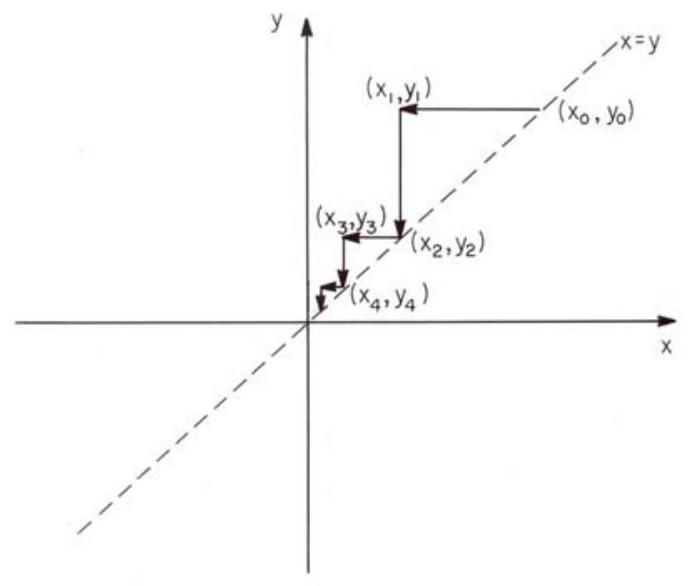
\includegraphics[max width=\textwidth, center]{2025_02_07_204a351db2d7f48b61ebg-102}

Figure 6.11: Simple steepest descent minimization of the function $f(x, y)=x^{2}+(x-y)^{2}$

The gradients in GOSIA are evaluated numerically, using the forward-difference formula or, optionally, the forward-backward approximation. While the forward difference formula


\begin{equation*}
\frac{\delta f}{\delta x_{i}}=\frac{f\left(x_{1}, x_{2}, \ldots x_{i}+h, \ldots\right)-f\left(x_{1}, x_{2}, \ldots x_{i}, \ldots\right)}{h} \tag{6.91}
\end{equation*}


requires only one calculation of the minimized function per parameter, in addition to the evaluation of the central value $f\left(x_{1}, x_{2}, \ldots x_{n}\right)$, the forward-backward formula


\begin{equation*}
\frac{\delta f}{\delta x_{i}}=\frac{f\left(x_{1}, x_{2}, \ldots x_{i}+h, \ldots\right)-f\left(x_{1}, x_{2}, \ldots x_{i}-h, \ldots\right)}{2 h} \tag{6.92}
\end{equation*}


requires two calculations of the minimized function per parameter. The forward-backward formula then should be requested only in the vicinity of the minimum, where the accuracy of the numerical calculations starts to play an important role.

\subsection*{6.7.5 Gradient + Derivative Minimization}
The steepest descent minimization is efficient if a minimized function is smooth in the space of parameters, but it exhibits considerable drawbacks when dealing with functions having sharp "valleys" superimposed on smooth surfaces. Such valleys are created by strong correlations of two or more parameters. In the case of Coulomb excitation analysis, the valleys are introduced mainly by including accurate spectroscopic data, especially branching ratios, which fix the ratio of two transitional matrix elements. Note, that even if the branching ratio is not introduced as an additional data point, the valley still will be present in the yield component of the least-squares statistic $S$ if yields for both transitions depopulating a given state are observed. To demonstrate this deficiency of the simple steepest descent method, let us consider a model situation in which a two-parameter function $f(x, y)=x^{2}+(x-y)^{2}$ is minimized, starting from a point $x=y$. The term $(x-y)^{2}$ creates a diagonal valley leading to the minimum point $(0,0)$. Using the analytic gradient and the stepsize given by 6.84 , it is seen that the minimization using the steepest descent method will follow a path shown in figure 6.10 instead of following the diagonal.

To facilitate handling of the two-dimensional valleys, introduced by the spectroscopic data, GOSIA offers a gradient+derivative method, designed to force the minimization procedure to follow the two-dimensional valleys, at the same time introducing the second-order information without calculating the second order matrix (6.85), thus speeding up the minimization even if the minimized function has a smooth surface. Generally, to minimize a locally parabolic function:


\begin{equation*}
f(\bar{x})=f\left(\bar{x}_{0}\right)+\bar{\nabla}_{0} \Delta \bar{x}+\frac{1}{2} \Delta \bar{x} J \Delta \bar{x} \tag{6.93}
\end{equation*}


one can look for the best direction for a search expressed as a linear combination of an arbitrary number of vectors, $\bar{P}_{i}$, not necessarily orthogonal, but only linearly independent. This is equivalent to requesting that:


\begin{equation*}
f\left(\bar{x}_{0}-\sum_{i} \alpha_{i} \bar{P}_{i}\right)=\min \tag{6.94}
\end{equation*}


with respect to the coefficients $\alpha_{i}$. Merging 6.89 and 6.90 gives:


\begin{equation*}
f\left(\bar{x}_{0}\right)-\sum_{i} \alpha_{i}\left(\bar{\nabla}_{0} \cdot \bar{P}_{i}\right)+\frac{1}{2} \sum_{i j} \alpha_{i} \alpha_{j} \bar{P}_{i} \bar{J}_{j} \bar{P}_{j}=\min \tag{6.95}
\end{equation*}


which can be written in the vector form as:


\begin{equation*}
f\left(\bar{x}_{0}\right)-\bar{\alpha} \cdot \bar{\beta}+\frac{1}{2} \bar{\alpha} R \bar{\alpha}=\min \tag{6.96}
\end{equation*}


with a set of coefficients $\alpha_{i}$ treated as a vector $\bar{\alpha}$ and with:


\begin{align*}
\beta_{i} & =\bar{\nabla}_{0} \cdot \bar{P}_{i}  \tag{6.97}\\
R_{i j} & =\bar{P}_{i} J \bar{P}_{j}
\end{align*}


The matrix $R$ is symmetric following the symmetry of $J$, thus the solution for the vector $\bar{\alpha}$ is given by:


\begin{equation*}
\bar{\alpha}=R^{-1} \bar{\beta} \tag{6.98}
\end{equation*}


The gradient+derivative minimization algorithm uses two directions - the gradient, defining a direction of steepest descent, and a derivative of the gradient with respect to the displacement along its direction:


\begin{equation*}
\bar{D}=\lim _{h \rightarrow 0} \frac{\bar{\nabla}\left(\bar{x}_{0}+h \bar{\nabla}_{0}\right)-\bar{\nabla}_{0}}{h} \tag{6.99}
\end{equation*}


It can be shown that as long as the quadratic approximation 6.91 is valid:


\begin{equation*}
\bar{D}=J \bar{\nabla}_{0} \tag{6.100}
\end{equation*}


Using the identity resulting from the symmetry of $J$ :


\begin{equation*}
\bar{\nabla}_{0} J^{2} \bar{\nabla}_{0}=\left(J \bar{\nabla}_{0}\right)^{2} \tag{6.101}
\end{equation*}


gives:

\[
R=\left|\begin{array}{cc}
\bar{\nabla}_{0} \bar{D} & \bar{D}^{2}  \tag{6.102}\\
\bar{D}^{2} & \bar{D} J \bar{D}
\end{array}\right|
\]

where all terms, except $R_{22}$, are known. By sampling the minimized function this missing term can be expressed as:


\begin{equation*}
\bar{D} J \bar{D}=\frac{2}{h^{2}}\left[f\left(\bar{x}_{0}+h \bar{D}\right)-f\left(\bar{x}_{0}\right)-h \bar{\nabla}_{0} \cdot \bar{D}\right] \tag{6.103}
\end{equation*}


The coefficients $\alpha_{1}$ and $\alpha_{2}$, resulting from the solution of 6.94 , can be rescaled arbitrarily, since we are only interested in the direction of search, the stepsize being found by the one-dimensional minimization procedure outlined in a previous section. A most convenient representation of a direction of search $\bar{\nabla}$, renormalized to avoid numerical overflows, is given by:


\begin{equation*}
\bar{\nabla}=\left(\frac{\bar{D} J \bar{D}}{|\bar{D}|^{3}}-\frac{\bar{\nabla}_{0} \cdot \bar{D}}{\left|\bar{\nabla}_{0}\right|^{2}|\bar{D}|}\right) \bar{\nabla}_{0}+\frac{1}{|\bar{D}|}\left(\frac{\left(\bar{\nabla}_{0} \bar{D}\right)^{2}}{\left|\bar{\nabla}_{0}\right|^{2}|\bar{D}|^{2}}-1\right) \bar{D} \tag{6.104}
\end{equation*}


Although primarily designed to accommodate the narrow valleys superimposed on the least-squares statistic by spectroscopic data, the gradient+derivative method usually gives much better results than the\\
simple steepest descent, providing faster fitting despite the necessity of calculating two sets of derivatives per step of minimization. Since two linearly independent vectors define a two-dimensional space, the gradient+derivative method is very suitable to deal with the decoupled correlated pairs of matrix elements (note that, as could be expected, the solution of the model case discussed above then is found in a single step of minimization).

\subsection*{6.7.6 Quadratization of the $S$ Statistic by Redefinition of the Variables}
The minimization methods outlined in previous subsections are built on the assumption that the minimized function can be described locally by the first or second order approximation, therefore their efficiency is strongly dependent on the extent to which this assumption is justified. Generally, the Coulomb excitation data analysis problem cannot be parametrized in such a way that the least-squares statistic $S$ (6.73) becomes strictly a quadratic function. Some hints as how to improve the efficiency of minimization come, however, from considering extreme cases, most important of which is a perturbation-type process, characterized by direct dependence of the excitation probabilities on the product of squares of the matrix elements directly connecting a given level to the ground state. Assuming a cascade-like decay with negligible feeding from above and negligible branching, the $\gamma$-decay intensities are expected to be proportional to the product of squares of the level-dependent subsets of transitional matrix elements, thus the $\gamma$-yields part of the $S$ statistic can be expressed as a quadratic function of the logarithms of $\gamma$-ray yields versus the logarithms of the matrix elements (note that the same holds for the spectroscopic data, although the signs of the $E 2 / M 1$ mixing ratios and known $E 2$ matrix elements are to be disregarded). While expressing the dependent variables on a logarithmic scale is straightforward, the same operation for the matrix elements would mean enforcing a sign identical to that of the initial guess. To avoid this problem, the logarithmic transformation of the matrix elements is only taken to first order of Taylor expansion, resulting in the actual minimization still performed in the matrix elements space with the direction of search being modified. To derive such an approach, let us consider the modification of a single matrix element, $M$, having an initial value of $M_{0}$, during a single step of minimization. A transformation to the logarithmic scale yields the transformed derivative of a minimized function $f$ with respect to $M$ :


\begin{equation*}
\frac{\delta f}{\delta \ln M}=\left|M_{0}\right| \frac{\delta f}{\delta M} \tag{6.105}
\end{equation*}


which, using the steepest descent method, gives a new value of $M$ according to:


\begin{equation*}
\ln |M|=\ln \left|M_{0}\right|-h\left|M_{0}\right| \frac{\delta f}{\delta M} \tag{6.106}
\end{equation*}


Expanding $\ln |M|$ into a Taylor series around $M_{0}$ and retaining only the first order term gives:


\begin{equation*}
M=M_{0}-h M_{0}^{2} \frac{\delta f}{\delta M} \tag{6.107}
\end{equation*}


which defines the modified direction of the search. When the gradient+ derivative method is used, both vectors must be combined according to equation 6.98 and multiplied by $\left|M_{0}\right|$ to obtain the transformed direction of the search.

A scale change of the matrix elements is, in principle, mainly justified if the logarithmic scale is simultaneously used for the dependent variables ( $\gamma$-ray yields etc.). However, even if the dependent variables are not transformed, the change of scale for the matrix elements, resulting in relative, rather than absolute, variations, can improve the efficiency of the minimization. A typical situation in which fitting the relative changes is efficient is when a strong dependence on a small matrix element determines the stepsize, $h$, common for a whole set, thus inhibiting the modification of much larger matrix elements if the absolute changes are used. Using the relative changes, however, one brings the sensitivity to all matrix elements to a common range, thus improving the simultaneous fit.

The minimum of a logarithmically transformed $S$ function does not, in general, coincide with the minimum of the original least-squares statistic. The minimization procedure uses only the direction of search resulting from the transformation of the dependent variables, if requested, still monitoring the original $S$ statistic. The transformation of the dependent variables therefore should be switched off when the current solution is close to the minimum of $S$.

\subsection*{6.7.7 Selection of the Parameters for Minimization}
The gradient-type minimization, as used in GOSIA, tends to vary the parameters according to their influence on the least-squares statistic $S$. It is easily understandable, since the most efficient decrease of $S$ primarily is obtained by varying the parameters displaying the strongest influence, measured by the current magnitude of the respective components of a gradient. With the stepsize, $h$, being common for the whole set of parameters, it is clear that unless the strong dependences are already fitted (which results in reduction of their derivatives) the weak dependences practically will not be activated. This is a serious concern in Coulomb excitation analysis, since the sensitivity of the $S$ function to different matrix elements can vary by orders of magnitude. The attempt to perform the minimization using a full set of the matrix elements usually means that most of them will come into play only after some number of steps of minimization but all the necessary derivatives are to be calculated from a very beginning, enormously increasing the time spent on computation without any significant improvement compared to the much faster minimization performed initially for only a subset of matrix elements. To speed up the process of fitting, GOSIA offers a wide range of both user-defined and automatic ways of reducing a number of parameters according to the current status of the minimization. The user may decide first to fix some of the matrix elements included in the initial setup, but found to have no influence on the processes analyzed. Secondly, the user may specify a subset of the matrix elements to be varied during a current run overriding the selection made initially. The selection of the free variables for a current run also can be made by the minimization procedure itself, based on the magnitudes of the absolute values of the gradient components evaluated during a first step of the minimization compared to the user-specified limit. The direction of the search vector, being either a gradient or a gradient+derivative vector, is always normalized to unity, allowing the user to define the limit below which the matrix elements will be locked for a current run if the absolute values of the respective derivatives are below this limit. In addition, some precautions are taken against purely numerical effects, most notably against the situation in which numerical deficiency in evaluating the derivative causes a spurious result. The minimization procedure in GOSIA stops if either of three user-defined conditions is fulfilled: first, the value of the $S$ function has dropped below the user-specified limit; second, the user-specified number of steps has been exceeded; third, the user-given convergence limit has been achieved, i.e. the difference between two subsequent set of matrix elements (taken as a length of the difference vector) is less than this limit. The first two conditions fulfilled terminate a current run, while, after the convergence limit has been hit, the minimization is resumed if it was specified to lock a given number of the matrix elements influencing the $S$ function to the greatest extent to allow the weaker dependences to be fitted (the details of the usage of the user-defined steering parameters are given in Chapter 7). To further reduce the numerical deficiency, GOSIA monitors the directions of two subsequent search vectors and fixes the matrix element having the largest gradient component if two subsequent directions are almost parallel, which usually signifies that a spurious result of the numerical differentiation of $S$ with respect to this matrix element inhibits the fitting of the less pronounced dependences. A warning message is issued if this action was taken.

An additional reduction of the free variables can be done by coupling of the matrix elements, i.e. fixing the ratios of a number of them relative to one "master" matrix element. This feature is useful if the experimental data available do not allow for a fully model-independent analysis, therefore some model assumptions have to be introduced to overdetermine the problem being investigated. The "coupled" matrix elements will retain their ratios, as defined by the initial setup during the fitting, a whole "coupled" set is treated as a single variable.

Finally, GOSIA requires that the matrix elements are varied only within user-specified limits, reflecting the physically acceptable ranges. The matrix elements are not allowed to exceed those limits, neither during the minimization nor the error calculation.

\subsection*{6.7.8 Sensitivity Maps}
As a byproduct of the minimization, GOSIA provides optional information concerning the influence of the matrix elements on both the $\gamma$-ray yields and excitation probabilities. The compilation of those maps is, however, time-consuming and should be requested only when necessary. The yield sensitivity parameters, $\alpha_{k i}^{y}$, define the sensitivity of the calculated $\gamma$-ray yield $k$ with respect to the matrix element $i$ as:


\begin{equation*}
\alpha_{k i}^{y}=\frac{\delta \ln Y_{k}}{\delta \ln \left|M_{i}\right|}=\frac{M_{i} \delta Y_{k}}{Y_{k} \delta M_{i}} \tag{6.108}
\end{equation*}


The excitation probability sensitivity parameters, $\alpha_{k i}^{p}$, are expressed similarly, the yields being replaced by the excitation probabilities The code allows the six most pronounced dependences to be selected for each experimentally observed yield for the printout, while a number of the matrix elements for which the most important probability sensitivity parameters are printed out can be selected by the user.

By definition, the sensitivity parameters provide (to the first order) a relationship between the relative change of the excitation probabilities, $p$, (or the calculated $\gamma$-ray yields) and the relative change of the matrix elements according to:


\begin{equation*}
\frac{\Delta p_{k}}{p_{k}}=\alpha_{k i}^{p} \frac{\Delta M_{i}}{M_{i}} \tag{6.109}
\end{equation*}


thus supplying locally valid information on the dependence of experimental data on matrix elements. An identical relationship holds for the yield sensitivity parameters, although the code calculates them only for the $\gamma$ detector labeled as $\# 1$ for each experiment, thus the angular distribution of the $\gamma$ rays, affected for example by the mixing ratios, is not accounted for fully. It is suggested that a $\gamma$-ray detector yielding the most complete and accurate yields should be defined as the first one in the description of an experiment to ensure that the yield sensitivity maps are calculated for all the yields observed.

The sensitivity parameters are not strongly dependent on the actual matrix elements, therefore the sensitivity maps can be treated as an indication of the features of the excitation/deexcitation process at any stage of minimization. As an extreme case, it should be noted that if the lowest-order perturbation theory applies, i.e. the excitation probability of a given state is proportional to the product of the squares of matrix elements connecting this state with the ground state, then the probability sensitivity parameter will equal 2 for all such matrix elements and will vanish for all others, no matter what are the actual value of the matrix elements. The same holds for the yield sensitivity parameters, provided that the $\gamma$-ray decay follows a simple cascade with no branching (the feeding from above can be neglected as a consequence of assuming the applicability of the lowest-order perturbation approach).

The sensitivity maps provide useful information that can be used during fitting to define the current sets of correlated matrix elements to be varied, to check to what extent the different sets of experimental data are independent and, finally, to ascertain which matrix elements included in the initial setup have a significant influence on the processes analyzed. The data obtained during the compilation of the yield sensitivity map also are used to generate the correlation matrix, selecting the subsets of matrix elements that are strongly correlated for the error estimation (see Section 6.8). It should be noted, however, that the compilation of the sensitivity maps is time-consuming, thus it should be requested only periodically when needed. The sensitivity maps also are helpful when planning an experiment, in which case a set of simulated $\gamma$-ray yields can be used as experimental data for a dummy minimization run. Simulated yields can be created by GOSIA using OP,POIN - see 7.19 or using the GUI Rachel which uses full intergation to simulate data with simulated statistical errors. A comparison of the sensitivity parameters for different (existing or planned) experiments give an indication to what extent the additional sets of data provide qualitatively new information.

\subsection*{6.8 Estimation of Errors of the Fitted matrix Elements}
\subsection*{6.8.1 Sources of Systematic Error}
The following sources of systematic errors could influence the results extracted using Gosia to analyze Coulomb excitation data.\\
a) Coulomb-nuclear interference

As discussed in chapter 2.1.1, the basic assumption of Coulomb excitation is that the interaction is purely electromagnetic. Multiple excitation of the highest spin members of collective bands requires use of the maximum allowed bombarding energies, thus it is crucial to know the maximum bombarding energy for which the interaction is purely electromagnetic. Experimental data on the influence of Coulomb-nuclear interference effects on measurements of excited state static quadrupole moments provided an estimate of the maximum bombarding energy at which the influence of nuclear excitation can be neglected. These data suggest that for heavy ions the influence on the cross sections is $<0.1 \%$ [CLI69a][CLI69b] if the classical distance of closest approach of the Rutherford trajectory for a head-on collision exceeds $\left[1.25\left(A_{p}^{1 / 3}+A_{T}^{1 / 3}\right)+5\right] f m$. This classical safe bombarding energy criterion is only applicable if the semiclassical approximation is valid, and corresponds to bombarding energies below 4.5 MeV per nucleon for ${ }^{208} \mathrm{~Pb}$ ions decreasing to less than 4.1 MeV\\
per nucleon for ${ }^{40}$ Ar ions. Coupled-channel Born Approximation codes, such as PTOLEMY[MA78, RH80], must be used for a more reliable estimate of the influence of Coulomb-nuclear interference for collisions involving nuclei lighter than ${ }^{16} \mathrm{O}$. A comparison [KAV90] of PTOLEMY calculations with GOSIA predictions for Coulomb excitation of ${ }^{76} \mathrm{Se}$ by ${ }^{208} \mathrm{~Pb}$ showed that a bombarding energy $7 \%$ above the safe bombardingenergy criterion resulted in destructive interference ranging in magnitude from $2 \%$ for the first $2^{+}$state to $10 \%$ for the weakly excited second $2^{+}$state.

\section*{b) Quantal Corrections}
The accuracy of the semiclassical approximation improves with increase of the Sommerfeld parameter $\eta$ defined in equation 2.2. The use of energy-symmetrized orbits in the semiclassical calculations partially corrects for deficiencies in the semiclassical approximation. The remaining quantal correction to the calculated cross sections are of the order of $1 / \eta$ for large $\eta$. Typically $\eta$ ranges from 50 to 500 for heavy-ion induced Coulomb excitation. Full quantal calculations by Kavka[KAV90] show that semiclassical calculations differ from full quantal predictions by typically $3 \%$, with some values as much as $10 \%$ off. These agree with the predictions of Tolsma [TOL79, TOL87] for the case of ${ }^{238} \mathrm{U}$ excited by $385 \mathrm{MeV}{ }^{84} \mathrm{Kr}$ ions. However, analysis of heavy-ion induced Coulomb excitation data typically involves a comparison of the deexcitation gamma-ray yields which tends to cancel part of this systematic error[KAV90, STA82].\\
c) Corrections to the Rutherford orbit

The Coulomb excitation probability is sensitive to the exact distance of closest approach of the classical Rutherford trajectory both for states involving large adiabaticity excitation, and also for many-step multiple Coulomb excitation. The distance of closest approach is proportional to the bombarding energy, thus it is important to have an accurate knowledge of the absolute bombarding energy of the incident beam. Most accelerator facilities quote the bombarding energy to many significant digits, but it behoves the experimenter to ascertain what absolute reference was used to calibrate the absolute beam energy. Integration over the energy loss in the target requires knowledge of the target thickness and nonuniformity which also contribute to the experimental error.

The classical Rutherford trajectory is perturbed slightly by atomic screening, vacuum polarization and relativistic effects. These effects slightly change the distance of closest approach which can be taken into account by making a small change in the bombarding energy used in the Gosia calculations. As illustrated in figure 2.9, these effects are small, and tend to cancel; i.e. the net correction to the bombarding energy typically is $<0.3 \%$ which is unimportant for most experiments[ALD75, KAV90]\\
d) Kinematic transformation from the laboratory to centre-of-mass frame of reference

As described in chapter 5.2, experimental data are recorded at fixed laboratory scattering angles whereas each Coulomb excitation calculation is performed for a given centre-of-mass angle. The transformation from the laboratory angle to the corresponding centre-of-mass angle is $Q$-value dependent and thus one must perform the Coulomb excitation calculation for each state separately using the state-dependent centre-ofmass angle corresponding to the laboratory scattering angle. This centre-of-mass angle dependence can lead to the largest systematic error when one of the interacting nuclei has a low mass, such as ${ }^{12} \mathrm{C}$, where the calculated Coulomb excitation cross section can change by about $3 \%$ per MeV change in $Q$-value. If both interacting nuclei are heavy, then this systematic error is small for normal kinematics, but for inverse kinematic reactions the correction is very large near the peak scattering angle of the two-valued solution for the scattered projectile.

\section*{e) Virtual excitation of unobserved states}
It is important to include explicitly, in the coupled-channel calculations, all states in the yrast domain that are likely to influence the results significantly. Unobserved states with excitation probabilities exceeding $0.1 \%$ can have measurable interference effects on the calculated population of observed states. Also the truncation of the coupled equations results in errors in the calculated cross section for the uppermost state in any collective band. Thus it is necessary to extend all collective bands by adding at least two buffer states beyond what is observed to ensure that virtual excitation and coupled-channel truncation effects are taken into account. The virtual excitation effects are reasonably insensitive to the exact excitation energies chosen for these unobserved states.

Moderate strength matrix elements coupling two nearly degenerate states can lead to appreciable effects even though there is no observable $\gamma$-ray deexcitation between them. Experience has shown that, in most nuclei, virtual excitation effects due to low-lying states can be estimated reliably and thus do not significantly add to the uncertainties in the final results.

Virtual excitation of the giant $E 1$ resonance can decrease the population of high-spin states by up to\\
$12 \%$ [CLI86]. Fortunately this can be estimated reliably by adding a polarization term to the interaction which is incoporated in GOSIA [ALD75].

\section*{f) Mutual excitation}
Both the target and projectile can be excited simultaneously influencing the cross sections for Coulomb excitation of a given state. Normally one of the two interacting nuclei is chosen to be a closed-shell nucleus, such as ${ }^{208} \mathrm{~Pb}$, to minimize such mutual excitation effects. Fortunately the multipole-multipole interaction term does not interfere with either monopole-multipole term, thus the corrections are small even for cases when mutual excitation is appreciable. For example, for the case of ${ }^{76} \mathrm{Se}$ excited by ${ }^{48} \mathrm{Ti}$ the predicted mutual excitation changes the ${ }^{76} \mathrm{Se}$ cross sections by only $0.7 \%$.[KAV 90 ]\\
g) Gamma-ray angular distributions

The hyperfine interaction of the excited nuclei recoiling in vacuum, that is the deorientation effect, contributes the largest uncertainty in predicting the angular distributions of the deexcitation $\gamma$-rays. The magnitude of the deorientation effect depends sensitively of the lifetimes of the deexciting states. Use of best-fit global parameters, within the framework of the Brenn and Spehl two-state model of the hyperfine interaction, has been shown to give a reasonable prediction of the deorientation effect [BOS77, BRE77]. Fortunately the uncertainty in our knowledge of the deorientation effect usually contributes $<2 \%$ error in the final extracted matrix elements, in part because the $\gamma$-ray detector arrays used in modern $4 \pi$ detector arrays average over the $\gamma$-ray angular distribution.

The assumption of cylindrical symmetry in evaluating the attenuation factors $Q_{\lambda}$, used to account for the finite size of the $\gamma$-ray detectors, is not applicable for clover-detector geometry used by some Ge detector arrays. However, use of the cylindrical symmetry assumption in general will introduce errors that are smaller than the uncertainties inherent in predicting the hyperfine interactions. The influence of using non-cylindrical $\gamma$-ray detectors can be tested by decomposing the detector into a raster of smaller cylindrical detectors.

States having lifetimes in the nanosecond range can decay while displaced significantly from the target spot due to the recoil. In most cases the first-order correction for in-flight decay available in Gosia is adequate to correct for this displacement.

\section*{h) Energy loss of ions in the target}
Chapter 5.3 pointed out that there are $\sim 15 \%$ descrepancies in the stopping power values derived from different compilations of heavy-ion energy loss in matter. In addition, non-uniformities in target thickness, density, possible crystalline structure, straggle, beam induced damage, and carbon build-up all can contribute systematic errors when comparing calculated with measured $p-\gamma$ yields. These sources of systematic error must be considered but the impact depends on whether absolute or relative yields are being used to extract matrix elements.

\section*{i) Absolute normalization of cross sections}
Comparison with the well-known Rutherford cross section for elastic scattering can be used to determine absolute Coulomb excitation cross sections. Although this approach is easy using the magnetic spectrometer technique[CLI69a], it is difficult when the higher sensitivity particle- $\gamma$ coincidence method is employed for heavy-ion Coulomb excitation work[CLI86]. The $\gamma$-ray detection efficiency typically is measured to an accuracy of $\approx 5 \%$ using well-known $\gamma$-ray sources. However, it is necessary to take ino account the coincidence detection efficiency which can be significantly reduced due to dead time and pile up rejection. An extreme example is the Coulomb excitation of the ${ }^{242} \mathrm{Am}$ isomeric target where the target activity resulted in a coincidence detection efficiency that was reduced by about $20 \%$ due to dead time and pile-up rejection[HAY07, HAY10].

Comparison of target-excitation with projectile-excitation $\gamma$-ray yields provides a simple approach for measuring relative $B(E \lambda)$ values in Coulomb excitation work. Another approach, that is applicable to strongly-deformed nuclei, is to normalize the measured deexcitation $\gamma$-ray yields to transitions at the bottom of the ground band which are populated predominantly by cascade feeding and thus are insensitive to the assumed matrix elements.

\subsection*{6.8.2 Statistical error estimation}
The most commonly used methods of estimating the errors of fitted parameters (in our case the matrix elements) resulting from a least-squares minimization, are derived using the assumptions that do not necessarily apply to Coulomb excitation analyses. Usually, the errors of the fitted parameters are evaluated either using the curvature matrix, or by requesting an increase of the least-squares statistic dependent on\\
the number of degrees of freedom and the value of this statistic at the minimum. An approach based on the second-order approximation is not applicable because this approximation is in general not valid even in the vicinity of the fitted set of matrix elements, not to mention the problems resulting from the so-called "nuisance parameters", i.e. parameters that can be introduced formally, but have no influence on the observed processes. The inclusion of such nuisance parameters prohibits a straightforward inversion of the second-derivative matrix. Moreover, the curvature matrix approximation assumes that the fit is perfect, i.e. the gradient at the solution point vanishes, thus only the second-order term describes the behavior of the least-squares statistic. Practically, however, we have to assume that a fitting procedure must be stopped at some point even though a number of the matrix elements that have a weak influence on the Coulomb excitation process, are far from their best values. This is not important from the point of view of extracting the information contained in the experimental data but can considerably disturb the error estimation of the significant dependences when the second-order approximation is used.

The unavoidable presence of the nuisance parameters also prohibits error estimation procedures based on the assumption that the least-squares statistic should obey the $\chi^{2}$ distribution with a given number of degrees of freedom. It should be noted that the concept of the number of degrees of freedom is implicitly based on the assumption that all the parameters are of about equal significance, which is obviously not true in the case of Coulomb excitation since the sensitivity of the observed $\gamma$ yields to the various matrix elements differs by orders of magnitude. This is illustrated by noticing that to describe a given experiment one can arbitrarily add any number of unobserved levels connected by any number of the matrix elements having no influence on either the Coulomb excitation or the $\gamma$ deexcitation, thus arbitrarily changing the number of parameters and, consequently, the number of degrees of freedom. Finally, any procedure based on the number of degrees of freedom will result in ascribing the errors of the fitted matrix elements according to the subjective feeling as to what is a valid parameter of the theory and what is not. The error estimation formalism used in GOSIA, described in subsequent sections, has been derived without employing either the local quadratic approximation or the concept of the degrees of freedom to provide a reliable (however in general non-analytic) method of calculating the errors of the fitted parameters.[LES71, LES10]

\subsection*{6.8.3 Derivation of the error estimation method}
Let us assume that a set of observables, $Y_{k}$, measured with known and fixed experimental errors, $\sigma_{k}$, is used to determine the values of a set of parameters, $x_{i}$. We also assume that the observables are related to the parameters by an error-free functional dependence, i.e. that if the experiments were error-free each experimental point $Y_{k}$ could be exactly reproduced as:


\begin{equation*}
Y_{k}=f_{k}(\bar{x}) \tag{6.110}
\end{equation*}


where $f_{k}$ stands for the functional description of the $k$-th observed data point using a given set of parameters, represented as a vector. However, since we have to assume the experimental uncerntainties, we can only determine the parameters by requesting that the least-squares statistic (as defined by 6.73) is minimized with respect to the set of parameters. In other words, the assumption that a set of $n$ parameters is sufficient to reproduce $N$ experimental observables $(N \geq n)$, is equivalent to assuming that only certain values of observed data forming an $n$-dimensional hypersurface in the space of observables are allowed, and the fact that the measured set of observables does not correspond exactly to any set of parameters is due only to experimental errors. From this point of view the extraction of the parameters based on a set of observables reduces to determining which point on a hypersurface of the "allowed" experimental values (referred to as a "solution locus") corresponds to the measured values. While the assignment of the closest point on a solution locus defines a "best" set of parameters (as shown below), the distribution of the probability that different points belonging to the solution locus actually represents the set of observables defines the errors ascribed to the parameters. It can be shown that both the "best" set of the parameters and the errors of the parameters can be found by examining the least-squares statistic if the "perfect theory" approach is assumed. Such an approach, actually employed in GOSIA, is presented below.

To simplify the notation, it is convenient to introduce the normalized observables, $y_{k}$, defined as:


\begin{equation*}
y_{k}=\frac{Y_{k}}{\sigma_{k}} \tag{6.111}
\end{equation*}


and to assume that the functional dependence also includes the normalization relative to the fixed experimental errors $\sigma_{k}$. Treating both the set of normalized observables and the set of normalized functional dependences as vectors, allows a compact definition of the unnormalized least-squares statistic, $\chi^{2}$, as:


\begin{equation*}
\chi^{2}=[\bar{f}(\bar{x})-\bar{y}]^{2} \tag{6.112}
\end{equation*}


where we have used a symbol $\chi^{2}$ to distinguish the unnormalized statistic from the normalized statistic $S$, as defined by Eq. 6.73. Assuming that the normalized observables, $y_{i}$, are independent and normally distributed (the width of the distribution is equal to unity, as a result of the normalization to the known experimental errors) one finds that the probability of the observed set $\bar{y}$ is an experiment-distorted reflection of a "true" set $\bar{y} \prime$ which is proportional to:


\begin{equation*}
P\left(\bar{y}^{\prime}\right) \approx \exp \left(-\frac{1}{2}\left(\bar{y}-\bar{y}^{\prime}\right)^{2}\right) \tag{6.113}
\end{equation*}


An assumption of the "perfect" theory allows only the "true" sets of experimental data which can be described by the functional dependence $\phi$, belonging to the solution locus. Therefore only the sets $\bar{y} \prime$ which can be expressed as:


\begin{equation*}
\bar{y}^{\prime}=\bar{f}(\bar{x}) \tag{6.114}
\end{equation*}


are to be taken into account. Substituting 6.110 into 6.109 gives:


\begin{equation*}
P(\bar{f}(\bar{x})) \approx \exp \left(-\frac{1}{2} \chi^{2}\right) \tag{6.115}
\end{equation*}


Note that in this "geometrical" picture, $\chi^{2}$ has the meaning of the square of the distance from the observed set of data to a point belonging to the solution locus, thus the least-squares minimization is equivalent to finding a point on the solution locus closest to the experimentally observed set of data. Such a point has the highest probability of reflecting an error-free measurement, as long as the assumption of a perfect theory is in effect. Equation 6.111 gives the probability that the observed set of data corresponds to a given point on the solution locus per element of volume of the solution locus. Thus the transition to a probability of a given set of parameters per unit of volume in the parameter space requires the density function, given by:


\begin{equation*}
\rho(\bar{x})=\frac{d V}{d x_{1} d x_{2} \ldots d x_{n}} \tag{6.116}
\end{equation*}


with $d V$ standing for the volume element of the solution locus as a function of the parameters $x_{i}$. The probability distribution in the parameter space can be subsequently written as:


\begin{equation*}
\frac{d P(\bar{x})}{d x_{1} d x_{2} \ldots d x_{n}}=C \rho(\bar{x}) \exp \left(-\frac{1}{2} \chi^{2}(\bar{x})\right) \tag{6.117}
\end{equation*}


with a normalization constant $C$ resulting from the condition that the integral of the probability distribution over the whole parameter space is equal to unity.

Eq. 6.113 defines the probability distribution of simultaneous assignment of a whole set of parameters. Practically, however, we are interested in ascribing the errors to individual parameters, therefore we have to reconstruct the one-dimensional probability distributions corresponding to individual parameters. Such a distribution for parameter $i$, with no assumptions made as to the "true" values of the remaining parameters, will be given by:


\begin{equation*}
\frac{d P\left(x_{i}\right)}{d x_{i}}=\int \frac{d P(\bar{x})}{d x_{1} d x_{2} \ldots d x_{n}} d x_{1} d x_{2} \ldots d x_{i-1} d x_{i+1} \ldots d x_{n} \tag{6.118}
\end{equation*}


the integration extending over all allowed values of the parameters except of the parameter $i$. Using equation 6.114 the error bars of a given parameter can be found by requesting that the probability that the "true" value of this parameter (evaluated by integrating the distribution 6.114) is contained within the error bars and is equal to an adopted confidence limit of $68.3 \%$; this corresponds to the confidence level for a standard deviation with the Gaussian distribution. Since, neither the minimum is perfect, nor the symmetry of $\chi^{2}$ around the minimum is assumed, it is reasonable to define upper and lower error limits independently. This is explicitly given by requiring that:


\begin{equation*}
\frac{\int_{x_{i}}^{x_{i}+\delta x_{i}} \frac{d P\left(x_{i}\right)}{d x_{i}} d x_{i}}{\int_{x_{i}}(\max )} \frac{d P\left(x_{i}\right)}{d x_{i}} d x_{i} \quad=0.683 \tag{6.119}
\end{equation*}


where $\delta x_{i}$ stands for the upper error limit, while $x_{i}(\max )$ denotes the maximum allowed value of $x_{i}$. A similar formula is used to determine the lower error limit with the maximum allowed value of $x_{i}$ replaced by the minimum allowed value of this parameter.

Until now the derivation of the error estimation formalism has rigorously followed the initial assumptions. The error estimation using equation 6.115 is, however, not practical when dealing with a multidimensional parameter space and non-analytic description of the functional dependence used to relate the parameters to the observed data. First, it is technically impossible to evaluate the density function, $\rho(\bar{x})$, if the analytic functional dependence is not known, as in the case of the multiple Coulomb excitation. It can be argued that if the parametrization of the processes observed is reasonable, the density function should be dependent only weakly on the actual set of parameters compared to the dependence of the $\chi^{2}$ function (otherwise, the parametrization would be unstable). Assuming that the $\chi^{2}$ exponent in equation 6.115 drops sharply in the vicinity of the error limit, while no drastic change of the density function takes place, one can take for granted that within a reasonable accuracy, the effect of weighting the Gaussian distribution with the density function can be safely neglected. Second, it is easily seen that the reconstruction of the one-dimensional probability distribution according to Eq. 6.114 is not feasible if the analytic form of the functional dependence is not known. Therefore it is necessary to adopt a "worst case" approach, i.e. to use an approximation yielding overestimated error bars but allowing a reduction of the multidimensional problem to a one-dimensional one without performing the numerical integration in the multidimensional space. To construct such an approach we introduce a concept of a "maximum correlation curve" defined as a curve in the parameter space for which an effect of varying a given parameter is, to the greatest extent, balanced by the changes of the correlated parameters to minimize an overall change of the $\chi^{2}$ function. Introducing the above approximations, the error criterion 6.115 can be rewritten as:

$$
\frac{\int_{x_{i}}^{x_{i}+\delta x_{i}} \exp \left(-\frac{1}{2} \chi^{2}\left(x_{i}\right) d l(\bar{x})\right)}{x_{i}(\max )} \exp \left(-\frac{1}{2} \chi^{2}\left(x_{i}\right) d l(\bar{x})\right) \quad=0.683
$$

where $l$ stands for the "maximum correlation" path and the probability distribution is treated as a function of the $i$-th parameter only; the dependence on other correlated parameters being defined by the path of integration, $l$. This simplification results in overestimation of the error bars, corresponding to the confidence limit of at least $68.3 \%$.

The error estimation formalism, presented above, fits well the needs of Coulomb excitation analysis. It is not sensitive to the redundant parameters, which will simply display no influence on the $\chi^{2}$ statistic. It allows introduction of physical limits for the matrix elements just by normalizing the probability distribution to its integral between those limits (note that in case of insignificant matrix elements, this will yield the errors of $68.3 \%$ of the full range - GOSIA issues a warning if the integration is stopped on the limit before the criterion 6.116 was fulfilled). Finally, note that neither the purely quadratic behaviour of $\chi^{2}$ nor the perfect minimum are explicitly assumed.

\subsection*{6.8.4 Numerical Estimation of Errors}
The error estimation in GOSIA is performed in two separate steps. First, the "diagonal" errors, i.e. the errors of individual matrix elements with all the others kept fixed, are found. This part of the error calculation is relatively fast and thus has been separated from the "full", or correlated, error estimation. The calculation itself consists of a straightforward numerical solution of equation 6.115, the fourth-order Runge-Kutta\\
integration method is used to numerically evaluate the integrals involved. The probability distribution is renormalized to its value at the central set of matrix elements to avoid under- and overflows, i.e. $\Delta \chi^{2}$ is used instead of $\chi^{2}$. As mentioned above, the diagonal error calculation is not very time-consuming, therefore it also can be used to speed up minimization provided that the strong influences were already fitted. Running the diagonal errors allows detection of the matrix elements that still are far from their best values judging from the pronounced asymmetries of the error bars. In addition, GOSIA notifies the user every time a better value of the statistic $S$ has been found. This information can be used to "manually" predict a better solution without performing a time-consuming minimization of the weak dependences. Also, in some cases, the improvement of $\chi^{2}$ found during the error calculation can be so large that the Gaussian distribution associated with the error estimation cannot be handled due to the machine-dependent overflow of the exponential involved. GOSIA detects such situations using a user-defined capacity of the computer, allowing to indicate which subsets of the matrix elements are to be refitted to improve the minimum.

The diagonal error calculation is usually repeated a few times until the minimum of the least-squares statistic $S$ is found to be satisfactory from the point of view of individual matrix elements. The following "full" error calculation differs from the diagonal error calculation only by applying Eq. 6.115 along the predicted path of maximum correlation. Although, in general, this path is a curve in the space of the parameters, we are forced, for practical reasons, to approximate it by a straight line. To make this approximation as reliable as possible, the information resulting from the diagonal error calculation is used by GOSIA to determine the way the probability distribution is sampled. An estimate of the diagonal error for a given matrix element is first used to evaluate an appropriate stepsize for the Runge-Kutta integration algorithm. Since the influence of a given matrix element is not known a priori, a common stepsize is used for the diagonal error estimation. This approach is subsequently refined by adjusting the stepsize for each matrix element individually during the full error calculation based on the diagonal error range. It may, in some cases, cause a slight decrease of the error range if there is no significant correlation and the stepsize assumed for the diagonal error calculation has incorrectly taken into account the sensitivity of the $\chi^{2}$ statistic to a given matrix element. The diagonal error bars also are used to define how the maximum correlation curve is approximated by a straight line in the space of the parameters. This operation is performed by assuming that the matrix element, for which the correlated error is estimated, is varied to the value corresponding to its central value $\pm$ an appropriate diagonal error and fixed at this value, while the one-step gradient minimization of the remaining matrix elements is done to find the correlation axis. The maximum correlation direction is then defined as a vector difference of the resulting set of the matrix elements and the central point. In this way, a correlation curve is approximated at a range consistent with the order of magnitude of the final error. However, it should be noted that performing the one-step gradient minimization to find the correlation axis is very time-consuming if all the matrix elements are taken into account. Moreover, since the gradient method will only affect the values of the matrix elements strongly correlated with the one investigated, the calculation of the derivatives with respect to all others is simply redundant and does not yield any improvement in predicting the correlation axis. To speed up the full error calculation, GOSIA offers a mechanism for reducing the number of matrix elements being taken into account, by predicting the subsets of mutually correlated matrix elements. This requires that at a final stage of minimization, the yield sensitivity map is compiled and the full set of the sensitivity parameters $\alpha_{k i}^{y}(6.104)$ is stored in a permanent file. A subroutine, OP,SELE (SELECT) uses the map of the sensitivity parameters to predict the correlation. Each two matrix elements are correlated if they affect the same data points, thus, for each matrix element $M_{l}$ the correlation with a matrix element $M_{k}$ can be measured by:


\begin{equation*}
c_{l k}=\sum_{i}\left|\alpha_{k i}^{y} \alpha_{l i}^{y}\right| \tag{6.121}
\end{equation*}


the summation extending over all observed $\gamma$-ray yields. The absolute values are taken to prevent the neglect of the correlation due to coincidental cancellation of opposite sign terms. For each matrix element, indexed by the row index $l$, OP,SELE identifies those matrix elements $M_{k}$ having values of $c_{l k}$ greater than $10 \%$ of the maximum value of $c_{l k}$ in this row. As a result, OP,SELE produces a binary matrix whose elements are either 0 , if no strong correlation was predicted, or 1 . The matrix elements explicitly correlated by the spectroscopic data are assumed to be correlated by definition. The correlation matrix then is used during the full error calculation to fix the matrix elements for which the correlation was not predicted when searching for the correlation axis.

GOSIA issues messages if lower values of the $S$ statistic have been found. The set of the matrix\\
elements producing an overall best value of $S$ is stored in a permanent file, which could be used eventually to improve the minimization as a starting guess. However, it should be remembered that the uncorrected fast approximation used during the error estimation can be a source of inaccuracies, thus the small changes in the $S$ statistic usually can be disregarded. If necessary an error estimate can be performed manually by making a $\chi^{2}$ fit to all the other parameters for a set of given values for the observable being determined.

\subsection*{6.8.5 Identification of Erroneous Data Points}
Fitting a large set of parameters, as in the case of Coulomb excitation analyses, one must be aware of the possible existence of local minima, which can cause the fitting procedure to be trapped in an erroneous $\chi^{2}$ minimum. While there is no general method of distinguishing a local minimum from a global one, some judgement is still possible based on the value of the normalized least-squares statistic $S$ and the comparison of experimental and fitted data. A local minimum could be created artificially by including erroneous pieces of data, such as incorrectly assigned $\gamma$ yields, or, even if there were no mistakes in the data, could result from the local dependence on the parameters. The information provided by GOSIA during the minimization and error estimation usually is sufficient to determine whether the solution is acceptable. To further facilitate the identification of the local solutions, GOSIA is equipped with a "troubleshooting" module, designed to detect inconsistencies within the data set. This module uses the information obtained at a current stage of minimization concerning the dependence of the observed $\gamma$ yields on matrix elements. Only the $\gamma$ yields observed in the detectors labeled $\# 1$ for each experiment are used, as a result of the convention that the $\gamma$ detector providing the most complete and reliable set of data should be defined as the first one. The troubleshooting routine first calculates the normalized $S$ statistic disregarding the other $\gamma$ detectors and the spectroscopic data, assuming the independent, code-calculated normalization, thus overriding the userspecified normalization constants. A large difference between a value of $S$ calculated this way, and the value resulting from the minimization, points to either a wrong relative normalization or a problem with reproduction of the $\gamma$-ray angular distribution, which may be due to the errors in assigning the angular positions of the $\gamma$ detectors ( inconsistencies within the spectroscopic data are easy to notice by comparing the calculated and experimental values). A next step is to select the experimental $\gamma$ yields data, which locally inhibit minimization with respect to the individual matrix elements. Keeping in mind the gradient method used for the minimization, it is easily seen that a "perfectly consistent" set of data used to form a least-squares statistic, which can be written in the form:


\begin{equation*}
\chi^{2}=\sum_{i} \delta_{i}^{2} \tag{6.122}
\end{equation*}


is characterized by the fact that all individual components of the derivative with respect to a given matrix element $M_{k}$


\begin{equation*}
\frac{\partial \chi^{2}}{\partial M_{k}}=2 \sum_{i} \delta_{i} \frac{\partial \delta_{i}}{\partial M_{k}} \tag{6.123}
\end{equation*}


should be of the same sign. This means that the overall direction found to improve the minimum with respect to this matrix element is the same as resulting from the separate pieces of data. Inconsistent pieces of data may, in turn, produce large terms of opposite sign, which consequently causes a small value of the derivative due to cancellation. In such a situation a given matrix element will not be varied. As a measure of this effect we introduce a parameter $r_{k}$, defined for each matrix element $M_{k}$ as:


\begin{equation*}
r_{k}=\log \frac{\sum_{i}\left|\delta_{i} \frac{\partial \delta_{i}}{\partial M_{k}}\right|}{\left|\sum_{i} \delta_{i} \frac{\partial \delta_{i}}{\partial M_{k}}\right|} \tag{6.124}
\end{equation*}


This parameter equals 0 if all the terms summed are of the same sign and becomes large when the cancellation effect is dominant. The numerator of 6.120 can be treated as an indication of the influence of a given matrix element $M_{k}$ (the "strength" of this matrix element) and is listed in the output of the troubleshooting routine separately. The routine further selects the data points having the largest positive and negative contributions to the derivative for all the matrix elements for which calculated $r_{k}$ exceeds an user-specified limit. This information may be helpful to pinpoint erroneous data points, e.g. missassigned $\gamma$\\
transitions. Sometimes, mostly for weakly overdetermined cases, local minima and saddle points may occur even if all the data are correct. The information provided by the troubleshooting module then can be used to modify the setup of the matrix elements to be fitted or inform the user to temporarily switch off some $\gamma$ yield data to allow the minimization procedure to find a way out of such an erroneous solution.

\section*{Chapter 7}
\section*{Input instructions for GOSIA}


\subsection*{7.1 Organization}
Input, execution and control of the code GOSIA is achieved by specifying a given sequence of option commands. These option commands are activated using the input format OP,- where - designates the fourcharacter alphanumeric name of the option command. Some options are used for input or selection of input needed for specific tasks, while other options execute appropriate modules of the code.

The code GOSIA can operate in either of two mutually exclusive modes. The first, activated by the option OP,COUL, performs the calculation of Coulomb excitation probabilities and $\gamma$-ray yields for a fixed set of the matrix elements. No fitting of matrix elements to experimental data is performed if OP,COUL has been selected. The other mode, activated by the command OP,GOSI, should be used if a least-squares fit of matrix elements to experimental data is desired. The user is free to use any other option commands in conjunction with either the OP,COUL or the OP,GOSI commands consistent with an obvious logic. For example, the code cannot calculate Coulomb excitation amplitudes if the level scheme is not defined, also it cannot execute the fit-related commands if OP,COUL has been selected. The input to the option commands OP,COUL and OP,GOSI contains "suboptions" for which the prefix OP, is not appended to the name. The suboptions must occur in a logical order to ensure that the required information has been input as illustrated in section 14.5 of this user manual. OP,GOSI can be used for any calculation as long as the differences between the format for OP,COUL and OP,GOSI are obeyed as noted in this chapter.

The many options built into GOSIA necessitate an input that is fairly extensive. The graphical user interface RACHEL (chapter 8) has been written to greatly facilitate preparation of the input as well as aid in presentation of the output of GOSIA. It is strongly recommended that GOSIA neophytes use the GUI, RACHEL, to quickly and easily generate an initial input and gain experience running GOSIA. Subsequently, the initial input generated by the GUI can be edited for cases that go beyond the capabilities built into RACHEL. Note that the GUI Rachel does not interpret gosia.inp files created by the user. Once you edit a gosia.inp file, you will usually have to abandon use of the GUI to continue calculations or fitting.

\subsection*{7.1.1 Input formats}
As a rule the input should be given in free format mode (READ*). This implies that the number of entries should correspond to the number of variables in the respective read list, different entries being separated by either a comma or a space. Floating-point values can be given as integers (the decimal point is not required and the conversion is automatic). Integers may not be given as floating point numbers. Blanks are not equivalent to zeros, unlike fixed-field formats, therefore zeros must be typed in explicitly. Some exceptions to this general input format will be stressed in the descriptions of various options. A wrong sequence of input entries is usually detected when a number is encountered instead of an expected alphanumeric option code. In this case a message UNRECOGNIZED OPTION - is issued and the job is aborted ( - designates\\
an unrecognized string ). This means that the sequence of the input entries is wrong somewhere between the last recognized option command and the entry reprinted.

\subsection*{7.1.2 Summary of available options}
A summary of all available options is given below. Detailed descriptions of each option and suboption command are given in alphabetical order in the subsection of this chapter listed next to the name of each option. Details of the file manipulation procedures are given in Chapter 10. The names of the option commands are truncated to four characters. Full, self-explanatory names are given in parentheses in the following description.

\section*{OP,BRIC (BRICC) (7.2):}
Activates calculation of the internal conversion coefficients for all transitions included in the matrix element file.

\section*{CONT (CONTROL) (7.3):}
Suboption of OP,COUL and OP,GOSI which is used to control and select various optional features of the code for both execution and output. This option can be omitted in which case default parameters will be used.

OP,CORR (CORRECT) (7.4)\\
Execution option to calculate the correction factors used to modify the experimental data to correct for the difference between the integrated yield calculations and the point values used for calculation of the Coulomb excitation cross sections and $\gamma$-ray yields during the $\chi^{2}$ fitting, as described in detail in 6.6.1.

\section*{OP,COUL (COULEX) (7.5):}
Activates the simple excitation/deexcitation mode. No fit of matrix elements to the data is made with this option in contrast to OP,GOSI. Consequently, the appreciable input required for the fit procedure can be skipped. OP, COUL contains the following suboptions:

\section*{LEVE}
(Section 7.14)\\
ME\\
(Section 7.16)\\
EXPT\\
Section 7.8)\\
CONT\\
(Section 7.3)

\section*{OP,ERRO (ERRORS) \\
 (7.6):}
Activates the error estimation module of the code. Also, it can be used to test the goodness of the solution, as discussed in detail in Chapter 6.8.

\section*{OP,EXIT (EXIT) (7.7):}
Terminates the job and causes the final output to be compiled.

\section*{EXPT (EXPERIMENT) (7.8):}
Suboption of OP,COUL and OP,GOSI which is used to input the experimental conditions for each of the experiments to be analyzed.

\section*{OP,FILE \\
 (FILES) \\
 (7.9):}
Optionally allows to declare archaic file names to be attached to the job in the input rather than in the job control stream.

\section*{OP,GDET}
(GE DETECTORS)\\
(7.10):

Creates the files that contain the data needed to calculate the solid angle attenuation factors (4.4). Output files should be attached to the job when OP,YIEL is encountered.

\section*{OP,GOSI (GOSIA) (7.11):}
This alternative option to OP,COUL is used when a fit of matrix elements is to be made to Coulomb excitation data. The suboptions for this option are the same as for OP,COUL (however, note that the input to ME differs from that used for OP,COUL):

\section*{LEVE}
(Section 7.14)

\section*{ME}
(Section 7.17)\\
EXPT\\
(Section 7.8)\\
CONT\\
(Section 7.3)

\section*{OP,INTG (INTEGRATE-1980)}
(7.12):

A deprecated execution option used to integrate the deexcitation $\gamma$-ray yields, resulting from Coulomb excitation, over energy loss of the incident beam in the target and over the solid angles of the particle detectors that uses the older input format. This is the original integration routine that has been superceded by OP,INTI and is included only for running legacy GOSIA inputs. Note that for inverse kinematics this option remains useful for those cases where only one of the two-valued solutions is needed.

\section*{OP,INTI (INTEGRATE-2008) (7.13):}
Execution option used to integrate the deexcitation $\gamma$-ray yields, resulting from Coulomb excitation, over energy loss of the incident beam in the target and over the solid angles of the particle detectors. This 2008 version of the integration routine supercedes OP,INTG. It is functionally identical to OP,INTG and solves a difficulty encountered when using inverse kinematics that also involves significant energy loss in the target, see chapter 6.5.2.

\section*{LEVE (LEVELS) (7.14):}
Suboption of OP,COUL and OP,GOSI which is used to read in and catalog the level scheme of the investigated nucleus.

OP,MAP (MAP) (7.15):\\
Causes the q-parameter maps ( 6.2 ) to be calculated and stored on an external file.

\section*{ME (MATRIX ELEMENTS OP,COUL Version)}
Suboption of OP,COUL which is used to input and catalog the matrix elements.

ME (MATRIX ELEMENTS OP,GOSI Version)\\
Suboption of OP,GOSI which is used to establish the matrix element setup for fitting.

OP,MINI (MINIMIZE) (7.18):\\
Executes the least-squares fit of the matrix elements to the experimental data.

\section*{OP,POIN (POINT) (7.19):}
Execution option tomake "point" calculates of the Coulomb excitation and deexcitation $\gamma$-ray yields at fixed scattering angle and bombarding energy.

\section*{OP,RAND (RANDOM) (7.20):}
Used to overwrite a given set of matrix elements by a set of random matrix element starting values lying within specified limits. This is useful to ensure removal of bias in determining the least-squares minimum.

\section*{OP,RAW (RAW DATA) (7.21):}
Used to input data necessary if efficiency-uncorrected (raw) $\gamma$ yields and/or yields resulting from summing several $\gamma$ spectra are to be used as experimental data.

\section*{OP,RE,A (RELEASE A) (7.22):}
Releases all matrix elements previously fixed and voids all coupling of matrix elements for the current minimization run.

OP,RE,C (RELEASE C) (7.23):\\
Releases all previously fixed matrix elements but preseves couplings.

OP,RE, (RELEASE F) (7.24): Voids coupling of matrix elements while retaining fixed ones.

\section*{OP,REST (RESTART) (7.25):}
Causes the program to use, as a starting point, a set of matrix elements stored on diskin file 12 by a previous calculation in place of the set given as input.

\section*{OP,SELE (SELECT) (7.26):}
Creates the correlation matrix for use by OP,ERRO

\section*{OP,SIXJ (SIX-j SYMBOL) (7.27):}
Creates a table of Wigner 6-j symbols used by the sum rules code SIGMA ( Chapter 9 ). OP,SIXJ is case-independent, thus it can be executed without defining the level and matrix elements scheme. It can also be inserted anywhere in the input sequence.

\section*{OP,STAR (START) (7.28):}
Execution option to calculate only the point-value Coulomb excitation amplitudes and excitation probabilities, not the $\gamma$-ray yields. This comprises a subset and consequently an alternative to OP,POIN. This option can be used with either OP,COUL or OP,GOSI.

\section*{OP,THEO (COLLECTIVE MODEL ME) (7.29):}
Generates matrix elements according to the geometrical rotor model following the Bohr-Mottelson prescription.

\section*{OP,TITL (TITLE) (7.30):}
Reads in the user-given title to be reprinted as a header of the output (maximum 80 alphanumeric characters). Can be repeated if more than one line is needed.

\section*{OP,TROU (TROUBLE) (7.31):}
Performs an analysis at the local minimum to pinpoint erroneous experimental data. This option must be inserted immediately before OP,EXIT.

OP,YIEL (YIELDS) (7.32):\\
Used for input of data required necessary to calculate the $\gamma$-ray deexcitation of the Coulomb excited nucleus and fit matrix elements to the $\gamma$-ray yields. OP,YIEL is mandatory if OP,GOSI has been selected, in which case it is also used to specify additional spectroscopic information, i.e. branching ratios, mixing ratios, lifetimes and known $E 2$ matrix elements, as well as relative $\gamma$ detector efficiencies and upper limits of the unobserved transitions. The experimental deexcitation yields are supposed to reside on a separate permanent file attached to the job. See also chapter 7.33.

INPUT OF EXPERIMENTAL $\gamma$-RAY YIELDS\\
Section 7.33 describes the structure of the file containing the experimental $\gamma$-ray yields from Coulomb excitation.

\subsection*{7.2 OP,BRIC (BRICC)}
This option uses the National Nuclear Data Center database, BrIcc, to calculate the internal conversion coefficients for all E1, E2, E3, M1, and M2 matrix elements included in the OP,COUL, or OP,GOSI input files. In order that the matrix elements included in the calculation are defined, the OP,BRIC must follow either OP,COUL or OP,GOSI. A Gosia subroutine CONV generates all needed internal conversion coefficients in a table of the ICC values for each multipolarity for each transition.

Two lines of data occur after the OP,BRIC input command. The first is the filename of the BrIcc index file, and the second is the filename of the BrIcc.icc file. That is, the input looks like:

OP,BRIC\\
/usr/local/bricc-22/BrIccFOV22.idx\\
/usr/local/bricc-22/BrIccFOV22.icc\\
(Two BrIcc files have been installed in /usr/local/bricc-22. They can of course go elsewhere and the user may wish to use the "no hole" version of the ICC tabulation, or, in the future, a later version than V22).

The BrIcc command will generate a file on unit 29. You can set a filename in the usual way with OP,FILE. Unit 29 will contain a table with the following information for each transition matrix element.

$$
E N E R G Y \quad I C C(E 1) \quad I C C(E 2) \quad I C C(E 3) \quad I C C(M 1) \quad I C C(M 2)
$$

This table will also be output to unit 22 , the main output file if PRT, option 18,1 is set (the default) in sub-option CONT.

If the GOSIA input file already contains internal conversion data in OP,YIEL, it is simple to turn on or off the use of OP,BRIC by changing the sign of N1 to negative in OP,YIEL. No other changes need to be made to the input. The user-input internal conversion data can be restored by changing the sign of N1 to positive to restore compatibility to older GOSIA versions and removing the OP,BRIC option. In this case, the current version of GOSIA will interpolate the ICC data from the user-supplied data as in older versions, except that the cubic spline method now replaces the Lagrange method. Note that the use of the older Lagrange interpolation of the BrIcc tables can be unreliable near the K, L edges and can give unreliable values between meshpoints. The newer OP,BRIC approach gives much more reliable results since interpolation is done separately for each multipole eliminating the need to interpolate across K,L edges etc.

If a new input is being written for the current version of GOSIA, implement OP,BRIC as above, and enter a dummy sequence for internal conversion data as follows. (This is designed to preserve backward compatibility for older input files.) Enter the following records in OP,YIEL.

N1, N2\\
$E 1, E 2, E 3, \ldots E N 1$\\
as\\
$-1,0$\\
0.010

Since $N 2=0$, Gosia will expect no input ( 0 records) for I1, CC1(I1), $\mathrm{CC} 2(\mathrm{I} 1) \ldots$, and these fields must be omitted. Gosia will read all necessary internal conversion data from unit 29, rather than interpolating. The 0.010 is a dummy record.

If the level scheme or the transition multipoles are changed, it is necessary to re-run the input with OP,BRIC to generate a new set of coefficients for new energies or added transitions. OP,BRIC can be removed for subsequent runs, which is useful if the user desires to change one or more ICCs in unit 29 manually.

\subsection*{7.3 CONT (CONTROL)}
This suboption of either OP,GOSI or OP,COUL is used to override default settings of the job performance controls and to specify optional features of the program. CONT can be omitted if the default settings of the control parameters are satisfactory. CONT can be used anywhere in the OP,COUL and OP,GOSI input stream, usually as the last suboption specified. The input format is as follows:

CONT\\
Input control parameters needed for the job.\\
END, Marks the end of the CONT input. End must be followed by a comma and a blank line.\\
The control switches are specified by a three-character alphanumeric string followed by a comma and, in some cases, by a floating point number $X$ (as a convention, $X$ will be used as the initial symbol for floating point entries while symbols beginning with $I$ are specified to be integer). Even if $X$ has the meaning of an integer it should be entered as a floating point number, the conversion being done by the code. Some of the switches require additional input. The available control switches are as follows:

ACC,X. Sets the accuracy parameter used as an internal check of the Adams-Moulton routine to $10^{-X}$. The default value is $X=5$. The step-size is either doubled or halved depending on whether the maximum deviation is less than $0.02 \times 10^{-X}$ or greater than $10^{-X}$. Do not use too large a value of $X$, as it slows down the calculation considerably with little increase in accuracy for $X$ much larger than 6 . Instead use the switch INT, to achieve maximum accuracy. This input is deprecated in that it can cause erroneously large values of $a(\omega)$ leading to unreliable results. See 6.1 for details and 6.3 for the impact of the accuracy parameter on the adiabaticity limitations.\\
$\mathbf{A C P}, \mathbf{X}$. Sets the convergence test parameter for the $\exp (A)$ expansion (6.13) to $10^{-X}$. Default value is $X=5$.

CCF, This switch overrides OP,MINI or OP,ERRO commands and causes GOSIA to terminate execution after calculating and storing the internal correction factors. This allows splitting the minimization or error estimation jobs, which can be helpful when using unreliable or overloaded computer systems.

CRF, This option causes GOSIA to read in the internal correction factors from file1 instead of recalculating them. This is a valuable time saver for restarting the minimization and error calculations using the OP,REST command. The internal correction factors are stored on file1 automatically when calculated by the code.

CRD,X. This switch defines which experiments use circular particle detectors. CRD, simplifies the input to OP,INTG and OP,INTI. The additional input is as follows:

IE(1) The indices, according to the input sequence in EXPT, of those $X$ experiments\\
IE(2) involving circular detectors. Note that the axial symmetry option in the EXPT input should be used rather than CRD, if the circular detector is symmetric with respect to the $z$ (i.e. beam) axis.\\
IE(X)

DIP,X. Sets the $E 1$ dipole polarization parameter to $X / 1000$. (See equations $3.25-26$ ). Default value is 5 .

END, Mandatory CONT flag marking the end of CONT input. Must be followed by a blank line.

FIX, This switch provides the easiest way to override the matrix elements setup specified by the ME input. When FIX, is encountered all matrix elements are fixed and only those specified by subsequent input are released for minimization or error estimation. Further input required:

IM The number of matrix elements to be released.\\
$\mathbf{I}(\mathbf{1})$, Indices of the matrix elements to be released (defined by the sequence\\
$\mathbf{I}(\mathbf{2})$ of the ME input).

I(IM)\\
Using FIX, it is easy to reduce the number of free matrix elements without modifying the ME input.

FMI, Fast minimization switch. Causes the code to terminate the job immediately after the OP,MINI step was completed, without compiling the final output. FMI, provides substantial time saving when the final output is not needed since the compilation of the final OP,MINI output involves a full Coulomb excitation calculation. The remainder of the input, including the repeated OP,MINI commands is ignored if the FMI, switch has been selected. FMI, cannot be used when the SEL, switch is set.

INR, Independent normalization switch. Overrides the relative normalization of $\gamma$ detectors and different experiments as specified in OP,YIEL and EXPT inputs. With the INR, switch set, the code will calculate the best normalization factors (i.e. the ones providing the minimum value of $\chi^{2}$ for a given set of elements) for each single $\gamma$ detector independently.

\section*{INT, X.}
$\mathbf{I E}_{1}, \mathbf{I S}$, Overrides the default step size check parameter, IS, of the Adams-Moulton integration routine for specified experiments. The step size check is made every $I S$ steps, with a resultant possible change in integration stepsize. The default value is $I S=1$, thus the stepsize may be adjusted after each complete integration step. Setting $I S=1000$ effectively switches off the stepsize control since 1000 steps exceeds the $\mathbf{I E}_{X}, \mathbf{I S}_{X} \quad$ range of integration (according to 6.1 ), forcing the code to retain maximum accuracy.\\
$X$ has the meaning of the number of experiments for which the default is to be altered. Additional input consists of $X$ records, $I E_{n}$ being the experiment number and $I S_{n}$ the accuracy control parameter for this experiment. The experiments are numbered according to the sequence of the EXPT input, thus this control switch only can be used after the suboption EXPT definition.

LCK, This switch allows fixing a series of matrix elements without modifying the initial setup, e.g. it can be used to keep the matrix elements belonging to a given multipolarity fixed during minimization. It requires further input as follows:

\section*{I,I1 Ranges of matrix elements to be fixed. \\
 I,I1}
$\mathbf{0 , 0}$ Two zeros end input

NCM,X. Causes the kinematics calculation to be performed assuming the final state of the excited nucleus is the state with user-given index equal to $X$. with 2 . as the default value. The states of an excited nucleus are numbered according to the sequence of the LEVE input.

PIN,X. The PIN option is used when the charged particle detectory comprises an array of small circular heavy-ion detectors, such as PIN diodes. $X$ is the number of experiments. This is followed by

I,I1 $\quad I$ is the experiment number and $I 1$ is the number of PIN diodes for that experiment There should be $X$ such records

\section*{I,I1}
This should be followed by labelling these experiments as circular detector type using CRD. Small area square PIN diodes can be approximated as equivalent circular detectors; this is accurate enough and saves defining the complicated orientation of the squares in space. Rachel allows calculation for larger area non-circular detectors.

For the example of 2 experiments, each employing 30 circular diodes, the input sequence should be:

CONT\\
PIN,2.\\
1,30\\
2,30\\
CRD,2.\\
1\\
2

Note that, under both OP,INTG and OP,INTI, the detectors should be defined according to the circular detector input; in this case there will be $2 \times 30$ double records. That is, the circular detector input requires two lines for each detector. OP,INTG or OP,INTI then will perform a summation over the whole set of PIN diodes. The PIN switch tells the code that a specified experiment involves not a single detector but a number of them.

PRT, This overwrites the default output options specifying the printout. It requires additional input as follows:

I,I1 $\quad I$ is the print option code and $I 1$ is the user-specified setting\\
I,I1\\
$\mathbf{0 , 0}$ The $\mathbf{0 , 0}$ ends the input of the print options.

The following table lists all the available codes

\begin{center}
\begin{tabular}{|c|c|c|c|}
\hline
CODE & \( \begin{aligned} & \text { DEFAULT } \\ & \text { VALUE } \end{aligned} \) & \begin{tabular}{l}
OTHER \\
VALUES \\
\end{tabular} & CONSEQUENCES OF OPTION \\
\hline
1 & 1 & \( \begin{gathered} 0 \\ -1 \end{gathered} \) & \begin{tabular}{l}
Print out level scheme, input matrix elements and kinematics (1). 0 inhibits such printouts, while -1 can be used to suppress kinematics only. When 0 is selected, the sequence: \\
should be inserted before the LEVE and ME suboptions of either OP,COUL or OP,GOSI to set an appropriate flag. \\
\end{tabular} \\
\hline
2 & 1 & 0 & Reprint of experimental $\gamma$ yields to be fitted (1). 0 suppresses this printout. \\
\hline
3 & 1 & 0 & Prints out experimental branching ratios and a comparison of experimental and calculated values (1). 0 inhibits this printout. \\
\hline
4 & -2 & 0 or any positive integer & Prints out the yield sensitivity map ( $\alpha_{\gamma}$ parameters) (see 6.7.8) after every $I 1$ number of minimization steps if $I 1$ is positive. Note that compilation of this yields sensitivity map is time consuming since it requires the calculation of derivatives with respect to all matrix elements. Consequently, it should be compiled only when necessary. $I 1=2$ causes the compilation of this map when the OP,EXIT command is encountered after at least one execution of the OP,MINI command. $I 1=0$ specifies no compilation or printout of this sensitivity map. \\
\hline
5 & 11111 & Any positive integer & Prints out the value of $\chi^{2} / N$, where $N$ is the number of data points, after every specified $I 1$ number of minimization steps. If $I 1=1$ then $\chi^{2} / N$ will be printed after every step. \\
\hline
6 & 11111 & Any positive integer & Printout of the gradient will occur every $I 1$ minimization steps. Default value effectively inhibits this printout. \\
\hline
7 & 0 & 1 & Specifies printout of excitation amplitudes and population when OP,EXIT is encountered after at least one OP,MINI command (1). $I 1=0$ specifies no such printout. \\
\hline
8 & 1 & 0 & $I 1=1$ specifies a comparison of experimental and calculated yields. $I 1=0$ specifies no such printout. This table will not be compiled if FMI, switch was used, even if $I 1=1$. \\
\hline
9 & 1 &  & Unused - free to be assigned. \\
\hline
10 & 1 & 0 & $I 1=1$ specifies printout of the kinematics for each integration meshpoint. $I 1=0$ inhibits such printout. \\
\hline
11 & 1 & 0 & $I 1=1$ specifies printout of the $\gamma$ yields for each integration mesh-point. $I 1=0$ inhibits such printout. \\
\hline
\end{tabular}
\end{center}

\begin{center}
\begin{tabular}{|c|c|c|c|}
\hline
CODE & \begin{tabular}{l}
DEFAULT \\
VALUES \\
\end{tabular} & \begin{tabular}{l}
OTHER \\
VALUES \\
\end{tabular} & CONSEQUENCES OF OPTION \\
\hline
12 & 1 & 0 & $I 1=1$ specifies printout of the $q$-parameter maps. $I 1=0$ inhibits such printout. \\
\hline
13 & 1 & 0 & $I 1=1$ specifies printout of the normalization constants as defined in chapter 6.7.2. $I 1=0$ inhibits such printout. \\
\hline
14 & 1 & 0 & $I 1=1$ specifies printout of the deorientation effect attenuation coefficients. $I 1=0$ inhibits such printout. At least one minimization step using OP,MINI or an OP,GOSI calculation is required to print the deorientation coefficients $G_{K}$. In the output file, they are labelled "vacuum depolarization coefficients." \\
\hline
15 & 1 & 0 & $I 1=1$ specifies printout of the mean lifetimes. $I 1=0$ inhibits such printout. \\
\hline
16 & 0 & 1 & $I 1=1$ causes all possible calculated yields to be printed in the tables comparing the experimental and calculated yields. $I 1=0$ causes the printout of the experimental and calculated yields only for the observed transitions and unobserved transitions for which the calculated values exceed the upper limits specified in the OP,YIEL input. \\
\hline
17 & 0 & Any positive integer & Causes printout of the probability sensitivity maps (the $\alpha_{\mathrm{p}}$ parameters defined in 6.7.8). I1 specifies the number of matrix elements having the largest influence to be printed for each level with the corresponding $\alpha_{\mathrm{p}}$ values. \\
\hline
18 & 0 & 1 & Causes the printout of the interpolated internal conversion coefficients. $I 1=0$ inhibits this printout. \\
\hline
19 & 0 & 1 & $I 1=1$ causes the printout of the excitation amplitudes when executing commands other than OP,STAR (e.g. OP,INTG or OP,INTI). \\
\hline
20 & 0 & 1 & $I 1=1$ causes the printout of the efficiency-uncorrected yields and respective efficiencies if OP,RAW is used. This output is produced on file23. Note that the $\gamma$-ray energies printed out are Doppler-shifted, according to the user given geometry and calculated kinematics modified energies are used to calculate the detection efficiencies. \\
\hline
\end{tabular}
\end{center}

SEL, Creates file ( file18) containing the information needed by the program SELECT to generate the correlation matrix used for the error calculation - see the description of OP,MINI and OP,ERRO. This switch is only active when OP,MINI is executed with a default setting of the print parameter 4 (see the description of the print parameters defined by the PRT, switch above).\\
$\mathbf{S K P}, \mathbf{X}$ This causes the code to skip $X$ selected experiments during the minimization procedure, i.e., the code does not take into account the selected experiments. This switch can be quite useful since often a subset of the experiments is sensitive only to a subset of matrix elements. The SKP, X switch requires additional input:\\
$\mathbf{I}(\mathbf{1})$ The indices of experiments to be skipped (experiments\\
$\mathbf{I}(2)$ are numbered according to the sequence in which they appear in the EXPT input)

I(X)\\
SMR, This control switch causes the input file for the rotational invariant program SIGMA (See Chapter 9) to be generated when OP,ERRO is executed. This switch is ignored if OP,ERRO is not executed.

SPL,X. This control switch with $X=1$ causes the use of the cubic spline routine SPLINE plus SPLINT[PRE92] instead of the default Lagrange interpolation for integration of yields over particle energy, $\theta_{\text {mesh }}$ and other interpolated data. The use of the cubic spline routine is strongly recommended.

TEN, Causes GOSIA to write the statistical tensors in the system of coordinates defined by Fig. 3.1 on file17 when either OP,STAR or OP,POIN is executed. The tensors written are the pure Coulomb excitation tensors, as defined by 4.1, and can subsequently be used by external programs to examine the $\gamma$-decay process (e.g. to study the deorientation effect). The structure of the statistical tensors file is described in Chapter 10.

VAC, This switch is used when it is desired to change the default parameters used to evaluate the vacuum deorientation effect (chapter 4.2). It requires the following additional input:\\
$\mathbf{I}, \mathbf{X}(\mathbf{I})$ : where $I=1,2, \ldots, 7$ specifies the parameter to be overwritten, $X(I)$ being the new value. Two zeros end this input. The\\
parameters are defined as in table 4.1. The index value $I$ is as follows:

\begin{center}
\begin{tabular}{ccl}
$I$ & $X(I)$ & Default value \\
1 & $J_{1}$ & 3 \\
2 & $\Gamma$ & $0.02\left(p s^{-1}\right)$ \\
3 & $\Lambda^{*}$ & $0.0345\left(p s^{-1}\right)$ \\
4 & $\tau_{c}$ & $3.5(p s)$ \\
5 & $g$ & $Z / A$ \\
6 & $K$ & $6.10^{-6}$ \\
7 & $x$ & 0.6 \\
\end{tabular}
\end{center}

A common $g$ factor is assumed for all nuclear levels. Note that $g=Z / A$ often is a poor estimate. The known $g$ factors of the lowest states can be used to give a better estimate.

Since the lifetimes are given in picoseconds the field strength parameter $K$ is $10^{-12}$ times the true value in gauss (the default value corresponds to $6.10^{6}$ gauss). Note that suboption EXPT must occur in the input file before the CONT option VAC, otherwise EXPT will overwrite the values set by VAC.

The deorientation effect can be switched off (if, for example, the influence of deorientation on the result is to be tested) by specifying:

$$
\begin{aligned}
& \mathrm{VAC} \\
& 3,0 \\
& 6,0 . \\
& 0,0 .
\end{aligned}
$$

WRN,X. This switch causes a warning message to be printed with the comparison of experimental and calculated yields for those yields for which the experimental and calculated values differ by more than $X$ standard deviations. The default setting is $X=3$.

\subsection*{7.4 OP,CORR (CORRECT )}
This execution-only option requires no input other than the command itself. It uses the file of original experimental yields (see Section 7.33), read from file3, and writes on file4 a set of yields which have been modified to correct for the difference between the yields calculated using full integration and the yields calculated using "mean" values of the bombarding energy and scattering angle for each experiment (see Equation 6.45). The modified (corrected) experimental yields, on file4, then are used as data for the minimization and error estimation procedures. The OP,INTI and OP,CORR commands must be run as one job with the OP,CORR command following OP,INTI in the sequence of option commands. The values of the mean energy and scattering angle used for the point calculations are those specified for each experiment in the EXPT input.

Note that NTAP (specifying the file containing the experimental yields in OP,YIEL) must equal 3 when using the OP,CORR command (i.e. the file containing the original uncorrected experimental yields must be file3).

\subsection*{7.5 OP,COUL \\
 (COULEX )}
This option is used to calculate the Coulomb excitation cross sections and yields of deexcitation $\gamma$-rays when no fitting of matrix elements to data is required. This option essentially is a truncated version of OP,GOSI which it replaces when fitting of matrix elements to data is not desired. The advantage of OP,COUL over the alternate OP,GOSI is that the matrix element limits and some of the OP,YIEL input can be omitted. The OP,COUL command is used to input the information defining the nucleus studied and the experiments for which the Coulomb excitation calculations are to be performed. The OP,COUL command should occur immediately following OP,TITL since the input to OP,COUL is used by almost all modules of the program. The input to OP,COUL comprises four different sub-options:

LEVE Read and establish the level scheme of the investigated nucleus. See Section 7.14.\\
ME Read and catalog the matrix elements. See Section 7.16. Note that this sub-option input differs from that of the version used with OP,GOSI.

EXPT Input of experimental parameters. See Section 7.8.\\
CONT Used to control and select various optional features of the program for both execution and output.This suboption can be omitted in which case default parameters of the code will be used. See Section 7.3. A blank record is necessary to terminate the input to OP,COUL

\subsection*{7.6 OP,ERRO (ERRORS)}
The module of GOSIA activated by OP,ERRO is designed primarily for estimating the error bars to be assigned to the set of matrix elements corresponding to the minimum value of $\chi^{2}$. However, this option also can be helpful in checking the existence of better solutions by providing a relatively fast way of scanning the $\chi^{2}$ hypersurface. Error estimation is performed in two separate stages. First, the "diagonal",or uncorrelated errors must be determined, next, the diagonal errors are used in the estimate of the "overall", or correlated errors. This procedure is described in detail in Section 6.8. Section 14.4.10 shows the correct location of OP,ERRO in the input stream.

The input to OP,ERRO is as follows:

\section*{OP,ERRO}
IDF, MS, MEND, IREP, IFC, RMAX\\
where:\\
IDF Mode flag. $I D F=0$ sets diagonal error calculation mode, $I D F=1$ selects the overall error estimation.

MS,MEND The range of matrix element indices for which error estimation is to be performed, i.e. the calculation will be carried out for matrix elements with indices fulfilling $M S \leq I N D E X \leq$ $M E N D$. Note that $M S$ can be entered as 0 or $-1 . M S=0$ implies that the calculation will be performed for all matrix elements (excluding fixed ones : see below), thus providing a short form of specifying the full range. $M S=-1$ can be used only for "overall" error calculation ( $I D F=1$ ). This allows the user to select an arbitrary set of the matrix elements defined by additional input required only if $M S=-1$. In this case the input to OP, ERRO is as follows:

\begin{verbatim}
OP, ERRO
1,-1,0, IREP,IFC, RMAX
MS , MEND 1
MS ,MEND D
0,0
\end{verbatim}

where $M S_{i}$ and $M E N D_{i}$ define the range of matrix elements indices similarly to $M S$ and $M E N D$ when both are positive. $M S_{i}=M E N D_{i}$ selects a single matrix element. Two zeros terminate this portion of input. This feature allows repeating the overall error estimation for a subset of matrix elements or to include the matrix elements that previously have been skipped without modifying the ME setup. A given value of $M E N D$ is redundant if $M S=0$ or $M S=-1$ has been selected.

IREP\\
Repetition flag, assuming values of 0,1 or 2 . $I R E P=0$ implies a new calculation, i.e. no previously stored errors are read in and the error file will be created.\\
$I R E P=0$ should be used in conjunction with $I D F=0$ for a first calculation of the diagonal errors.\\
$I R E P=1$ causes previously stored errors to be read in and used for the continuation of the error estimation. The errors are stored on file file15, which is updated during each execution of OP,ERRO.\\
$I R E P=2$ means that the sum-rules file, file3, has already been created during a previous "overall" errors calculation and causes the code to read it in and update it during the current run. The CONT switch SMR, should be set for both creation and update of file3. Note that in this case the experimental yields must reside on file4 to avoid a multiple definition of the input/output files. File3 is created with $I R E P=1$ and updated with $I R E P=2$ only if SMR , was specified. $I R E P=2$ reduces to $I R E P=1$ if the SMR, switch was not encountered. Both file15 and file3 are required by the sum-rules code SIGMA - see Section 9.2.2. The proper combination of MS,MEND and IREP makes it possible to split the time-consuming error estimation into several runs which is important when running GOSIA on heavily loaded or unreliable computers.

Note that in OP,YIEL the input NTAP must equal 4.\\
IFC\\
$I F C=0$ specifies that the correlation matrix is to be used to reduce the number of matrix elements taken into account to calculate the correlated errors (see Section 4.6). The correlation matrix is created by the external program SELECT. To prepare the input information for SELECT it is necessary to execute OP,MINI with CONT switch SEL, and the default value of the print parameter 4 , i.e. $4,-2$. This should be done at a final stage of minimization prior to the error calculation. The information for SELECT is written by GOSIA on file18 which should be attached to SELECT also as file18. No other input is necessary. The output from SELECT is written on file 10 and should be attached to the OP,ERRO job as file18. $I F C=1$ implies that the correlation matrix will not be used. In this case it is not necessary to create and attach file18. It is however strongly recommended that $I F C=1$ be used only for small cases with all matrix elements of similar significance. Otherwise, selecting $I F C=1$ will dramatically increase the execution time with no effect on the result. $I F C$ is redundant if $I D F=0$.

RMAX The largest floating point number available on a given computer. RMAX is used to prevent possible overflows during the scan of a probability distribution (see 6.8).

Note: Fixed matrix elements will not be varied during the error calculation. Matrix elements usually should not be coupled when OP,ERRO is executed. Use release options (OP,RE,A and OP,RE,F) to remove couplings and unwanted fixing of matrix elements introduced in the ME setup.\\
N.B. Do not re-run the correlated error calculation without firsr re-running the diagonal error. Doing so will cause Gosia to over-estimate the errors because the output of the first stage (which should be the diagonal errors) is used to make an initial guess at the correlated error limits. Running OP,ERRO repeatedly to calculate correlated errors without repeating the diagonal error will approximately double the correlated error estimate each time.

\subsection*{7.7 OP,EXIT \\
 (EXIT)}
This option causes the code to terminate the execution and to compile the final printout as specified by the CONT PRT, print options. OP,EXIT may be inserted anywhere in the input stream and the execution will terminate after the completion of the last executable OP,- command encountered before OP,EXIT. The remainder of the input stream will be ignored, thus OP,EXIT allows to execute various modules of the code without removing the irrelevant portions of the input. No additional input is required.

\subsection*{7.8 EXPT (Mandatory suboption of OP,COUL and OP,GOSI)}
This suboption provides input of the experimental conditions used for the various experiments to be analyzed. The experiments are defined by mean values of projectile energy and scattering angle, which are used for "point" excitation/deexcitation calculations. The realistic approach must include integration of $\gamma$-ray yields over finite ranges of bombarding energy and scattering angles. This feature is provided by OP,INTI which should be used to reproduce observed $\gamma$ yields. As described in Chapter 6, GOSIA uses "point" energy and scattering angles to execute all modules except for the integration module activated by OP,INTI. The options OP,INTI and OP,CORR are used to convert experimental $\gamma$ yields to "point" values. Mean values of bombarding energy and scattering angle used by OP,CORR are the ones given in the EXPT input. EXPT should follow LEVE in OP,GOSI or OP,COUL.

The input to EXPT is as follows:

\section*{EXPT}
NEXP, $\mathbf{Z}_{1}, \mathbf{A}_{1}$

$$
\pm \mathbf{Z}_{n}, \pm \mathbf{A}_{n}, \mathbf{E}_{p}, \pm \boldsymbol{\theta}_{L A B}, \mathbf{M}_{c}, \mathbf{M}_{a}, \mathbf{I A X}, \phi_{1}, \phi_{2}, \text { IKIN }, \mathbf{L N}
$$

There need to be $N E X P$ records equal to the number of experiments. The experiments will be numbered by the code according to the sequence of these records from 1 to $N E X P$. A detailed explanation of entries is given below.

NEXP The number of experiments defined in the input. Each experiment corresponds to a particular combination of bombarding energy, scattering angle, experimental detector arrangement and ( $Z, A$ ) of the collision partner exciting the nucleus being investigated. ( $N E X P \leq 50$ ).\\
$\mathbf{Z}_{1} \quad$ Charge number of the investigated nucleus (Integer format).\\
$\mathbf{A}_{1} \quad$ Mass (in units of amu) of the investigated nucleus.\\
$\mathbf{Z}_{n} \quad$ Charge number of the uninvestigated nucleus (collision partner). A positive value signifies target excitation, i.e., $Z_{n}=Z_{\text {projecticle. }}$. A negative value signifies projectile excitation, i.e., $Z_{n}=Z_{t \arg \text { et }}$ (Integer format).\\
$\mathbf{A}_{n} \quad$ Mass (in the units of amu) of the uninvestigated nucleus (collision partner) $A_{n}$ will thus correspond to the projectile mass if $Z_{n}$ is positive and target mass if $Z_{n}$ is negative. A negative sign appended to $A_{n}$ signifies that this is a "thick" target experiment, that is, the beam is completely stopped in the target. This latter option has the time saving feature of switching off some irrelevant calculations such as the deorientation effect and recoil velocity correction.\\
$\mathbf{E}_{P} \quad$ The mean projectile bombarding energy, in the laboratory frame of reference, to be used for calculating the Coulomb excitation yields for the particular experiment. Input in units of MeV .\\
$\boldsymbol{\theta}_{L A B} \quad$ The mean scattering angle must be positive if the projectile is detected. A negative sign should be given with the true value of the projectile scattering angle if the recoiling target nucleus has been detected to ensure the selection of the proper kinematics. Note that by definition $\theta_{L A B}$ is always positive, the sign being only used by the code to set appropriate flags.\\
$\mathbf{M}_{C}$ Controls the number of magnetic substates to be included in the full Coulomb excitation calculations. For a given ground state polarization $M_{o}$, the magnetic substates in the range ( $M_{o}-M_{c}$, $M_{o}+M_{c}$ ) will be included for each level. Note that the sum total of magnetic substates for all levels must not exceed 1200. The code takes care of the obvious limitations in magnetic substates set by the spins of the states. $M_{c}=0$ corresponds to the conservation of magnetic quantum number as occurs for backscattering.\\
$\mathbf{M}_{A} \quad$ Controls the number of magnetic substates to be included in the approximate Coulomb excitation calculation. The meaning of $M_{A}$ is the same as for $M_{C}$, namely magnetic substates in the range $\left(M_{o}-M_{a}, M_{o}+M_{a}\right)$ will be included for all states for a given ground state polarization $\left.M_{o}\right)$. The only allowed values of $M_{a}$ are 0 or 1 .

IAX The axial symmetry flag which can take values of 0 or 1 only. Zero defines axial symmetry of the particle detector, in which case further input is simplified and the calculations are speeded up. Unity implies that axial symmetry is not assumed. (A sector of an axially-symmetric detector is considered to be asymmetric since the entire $2 \pi$ range of $\phi$ is not covered.)\\
$\phi_{1}, \phi_{2} \quad$ The azimuthal angular limits of the particle detector (in degrees). The coordinate system used has the $z$ axis in the direction of the incoming beam. The $x$ and $y$ axes can be defined in any convenient way provided that the angles of all detectors are given relative to the same cooordinate system. Note that $\phi_{2}$ must be larger than $\phi_{1}$.

IKIN The kinematics flag which can take values of 0 , and 1, only. IKIN specifies which of the two-valued kinematic solutions to choose for detection of scattered projectiles in experiments involving inverse kinematics. IKIN is redundant if $A_{\operatorname{Pr} \text { ojectile }}<A_{T \text { arg et }}$. When using OP,INTG the possible choices are given below.

IKIN The centre-of-mass scattering angles chosen corresponding to laboratory angles $\theta$\\
$0 \quad$ This selects the backward angle $\vartheta^{C M}$\\
1 This selects the forward angle $\vartheta^{C M}$\\
When using OP,INTI, then the IKIN input is ignored and selection of the solution is chosen internally by GOSIA.

LN Normalization constant control which specifies that the given experiment has a normalization constant coupled to that for experiment $L N$. The normalization constant is the factor normalizing the calculated yields to the experimental for a given experiment (See the description of the input YNRM in OP, YIEL, Section (7.32). Experiments are numbered according to the sequence of records read in under EXPT. Therefore, if $L N$ is equal to the record number defining a particular experiment then an independent normalization is assumed. If $L N$ does not equal the record number defining a given experiment then the program requires a user-given relative normalization between the current experiment and experiment $L N$ which is input using the OP,YIEL command. This input is useful for experiments where several scattering angles are measured simultaneously and therefore the relative normalization for the different scattering angles is known for this common experiment. The code will fit one absolute normalization constant to the coupled experiments. [Due to a design limitation in the current version, no target-detection experiment should be normalized to any other experiment, or vice-versa. For normal (not inverse) kinematics it is possible to overcome this restriction by specifying beam detection and giving the equivalent $\theta_{\text {beam }}^{l a b}$ range. For inverse kinematics it depends on whether both solutions are detected because of energy thresholds for the scattered particle.]

As an example consider two experiments to study ${ }^{72} \mathrm{Ge}$. One experiment involves Coulomb excitation of a ${ }^{72} \mathrm{Ge}$ target by a $50 \mathrm{MeV}{ }^{16} \mathrm{O}$ beam studied at a laboratory scattering angle of $160^{\circ}$ using an annular particle detector. The second experiment involves projectile excitation of a $170 \mathrm{MeV}{ }^{72} \mathrm{Ge}$ beam on a ${ }^{208} \mathrm{~Pb}$ target studied at a scattering angle of $150^{\circ}$ by a particle detector subtending an azimuthal $\phi$ range from $-30^{\circ}$ to $30^{\circ}$. The sample input is as follows:

EXPT\\
2,32,72\\
8,16,50,160,3,1,0,0,0,0,1\\
$82,208,170,150,3,1,1,-30,30,0,2$\\
Three magnetic substates are included for the full Coulomb excitation calculation and one magnetic substate for the approximate calculations for both experiments. Experiment 1 was done using an axially symmetric geometry, therefore $\phi_{1}$ and $\phi_{2}$ are redundant. Independent normalization of both experiments is desired; therefore, the $L N$ indices correspond to the experiment record numbers. In both cases $A_{\text {Pr ojectile }}<A_{T \arg \text { et }}$, thus IKIN is redundant.

\subsection*{7.9 OP,FILE (FILES)}
This option allows defining the permanent files necessary for a current job in the GOSIA input rather than in an external job control stream. The use of OP,FILE is optional, but when used it should be the first command in the input stream, so the full output goes to the user-defined file. The input to OP,FILE is as follows:

\section*{OP,FILE}
I1, I2, I3

\section*{NAME}
.\\
.\\
$0,0,0$\\
where:\\
I1 - Unit number (file number). $I 1=22$ is the ouput file.\\
I2 - Status indicator. $I 2=1$ indicates $S T A T U S=O L D, I 2=2$ implies STATUS $=$ NEW, while $I 2=3$ corresponds to STATUS $=$ UNKNOWN.

I3 $-I 3=1$ to indicate formatted file, $I 3=2$ means unformatted (binary) file. All files used by GOSIA are formatted, except of file1 (internal correction coefficients file) which should be declared as unformatted.

NAME - user-assigned filename.

\subsection*{7.10 OP,GDET (GE DETECTORS)}
This option is used to create a file (file9) which contains the data needed to reproduce the $\gamma$-energy dependence of the solid angle attenuation factors for the coaxial Ge or detectors (see Section 4.6). This option assumes cylindrical symmetry to calculate the angular distribution attenuation factors $Q_{k}$ using equations 4.49, 4.50. For each $\gamma$ detector a calculation following the formalism presented in Section 4.6 is carried out at several $\gamma$-energy meshpoints, then the energy dependence is fitted using a rational approximation according to Eq. 6.37. The fitted coefficients stored on file9 are automatically read in when OP,YIEL or OP,INTG is encountered. This means that OP,GDET should be executed once by itself before the execution of either OP,YIEL or OP,INTG. Section 14.4 shows the location of OP,GDET in the input stream.

The input to OP,GDET is as follows:\\
NPD The number of physically different $\gamma$ detectors being used for a whole set of experiments defined in EXPT. The physically identical detectors are understood as the ones having an identical crystal geometry and being placed at the same distance from the target. In addition, if graded absorbers were used, the physically identical detectors are assumed to be equipped with the same sets of graded absorbers where NPD $<50$. NPD should be given with a minus sign pre-pended if OP,RAW is to be used, i.e. if any of the experiments defined contains not efficiency-corrected spectra. In this case an additional file, file8, is created. file8 contains the absorber information, needed to reproduce the Ge detector $\gamma$-ray detection efficiency curves - see OP,RAW (7.21).

\section*{$\mathbf{r}, \mathbf{R}, \mathbf{L}, \mathbf{d}$}
$\mathbf{l}_{1}, \mathbf{l}_{2} \ldots \mathbf{l}_{7} \quad$ These two lines specify the geometry and the graded absorbers setup for each of the physically different detectors. This sequence should be repeated NPD times. All entries are given in centimeters.

The above entries are defined as follows:\\
$\mathbf{r} \quad$ The radius of the inactive p-core (the inner radius of a crystal).\\
$\mathbf{R} \quad$ The radius of the active n -core (the outer radius of a crystal).\\
$\mathbf{L} \quad$ The length of a crystal.\\
d The distance from a target to the face of a crystal.\\
$\mathbf{l}_{1} \ldots . \mathbf{l}_{7}$ The thicknesses of the commonly used graded absorber materials, with the subscripts 1 through 7 corresponding to $\mathrm{Al}, \mathrm{C}, \mathrm{Fe}, \mathrm{Cu}, \mathrm{Ag} / \mathrm{Cd} / \mathrm{Sn}, \mathrm{Ta}$ and Pb , respectively. The absorption coefficients for these materials are defined in GOSIA, for the energy meshpoints used, as internal data. It should be noted that if Ta or Pb absorber layers were used it is assumed that the $\gamma$ transitions having an energy below the cutoff of the absorption curve are of no interest, therefore the energy-dependence fit is made only using a subset of meshpoints corresponding to the $\gamma$ energies above 60 keV if $\mathrm{Cd} / \mathrm{Sn}$ layer was employed, above 80 keV if a Ta layer was employed and above 100 keV if a Pb layer was employed. It is also assumed that the symmetry axis of the crystal is aligned with the center of the target. Moreover, the effect of the in-flight decay, which changes the geometry as seen by a decaying nucleus, is not taken into account for the estimation of the solid angle attenuation factors. The significance of this correction is in all cases far below the level of the experimental accuracy.

The printout for OP,GDET lists $N P D, d$ (centimeters), and $E_{0}$. This is followed by a table with 3 columns and 8 rows which list $C_{1}, C_{2}$, and $Q_{k}\left(E_{0}\right)$ respectively for $k=1,2,3,4,5,6,7,8$. These values are defined by equation 6.37. All $Q_{k}(E)$ are zero when a $4 \pi \gamma$-ray detector is used. The $Q_{k}(E)$ can be set to zero by setting all the entries in the $Q_{k}\left(E_{0}\right)$ and $C_{1}$ columns to zero in the file on file9. Note that file9 file list is written in the order $C_{1}, C_{2}$ and $Q_{k}(E)$.

\subsection*{7.11 OP,GOSI}
(GOSIA)\\
This alternate option to OP,COUL is used when fitting matrix elements to Coulomb excitation data. The OP,GOSI command is used to input the information defining the nucleus studied and the Coulomb excitation experiments to be used in the least-squares fit procedure. The OP,GOSI command shall occur immediately following OP,TITL since the input to OP,GOSI is used by almost all the other option commands of this program. OP,GOSI requires the same input sequence of suboptions as OP,COUL, the only difference being that a different version of ME is used. That is, the input comprises the following four suboptions:

LEVE $\quad$ Read and establish the level scheme of the investigated (LEVELS) nucleus. See Section 7.14.

ME Read and catalog the matrix elements. See section 7.17. Important: note that the input to ME under OP,GOSI differs from the version used for OP,COUL. .

EXPT Input of experimental parameters. See Section 7.8..

CONT Used to control and select various optional features of (CONTROL) the program for both execution and output. This option can be omitted in which case default parameters of the code will be used. See section 7.3.

A blank record is necessary to terminate the input to OP,GOSI.\\
See also the additional changes to the OP,YIEL input when OP,GOSI is used.

\subsection*{7.12 OP,INTG (INTEGRATE-1980)}
The integrate command produces the most accurate calculation of the yields of deexcitation $\gamma$-rays following Coulomb excitation to be used for realistic comparison with experimental data. This option includes integration over solid angle of the particle detectors, energy loss in the target as well as full correction for the recoil velocity of the deexciting nucleus and the deorientation effect. This option also integrates the Rutherford scattering over the particle detectors and energy loss in the target which can be used as an absolute normalization.

OP,INTG is the original integration code written for GOSIA and still is available for running legacy inputs. In most cases it is strongly recommended that the 2008 upgrade code OP,INTI be used rather than the older code OP,INTG. The updated code OP,INTI was developed by Nigel Warr to handle problems that occur for integration of systems involving inverse kinematics when the recoiling target nucleus is detected. The OP,INTG and OP,INTI are identical except that the angle of the scattered projectile is input for OP,INTG whereas the angle of the detected particle is input for OP,INTI.

OP,INTG comprises two distinct stages. The first stage calculates the yields of deexcitation $\gamma$-rays integrated over azimuthal angle $\phi$ for each energy and centre-of-mass scattering angle meshpoint. This calculation of the meshpoint yields should be repeated for each experiment according to the order that the experiments appear in the EXPT input. GOSIA stores the calculated meshpoint yields as internal arrays. The second stage uses the data stored in these internal files to integrate over bombarding energy and the range of scattering angles subtended by the particle detectors which is performed by interpolating between the $\gamma$ yields calculated at each meshpoint. It is permitted to integrate over any arbitrary $(\theta, \phi)$ shape for the particle detector including the case of several $(\leq 4) \phi$ ranges for each $\theta$ value. An option is included to simplify integration over circular detectors because of the frequent use of such a geometry. The input for the circular detector is a slightly modified subset of the normal input.

It is strongly recommended that the $S P L, X$. option in CONT be set to\\
SPL, 1.\\
in order to select use of the cubic spline interpolation procedure. For more than 20 mesh points the Lagrange interpolation approach is unreliable since it diverges.

Note that $O P, G O S I$, including its four suboptions, plus $O P, Y I E L$, must occur in the input file prior to $O P, I N T G$ in order to provide the input necessary to run $O P, I N T G$. Note that for inverse kinematics OP,INTG can integrate only over one of the two center-of-mass solutions corresponding to an angular range in the laboratory system as specified in suboption $E X P T$ which can be a problem when the two solutions are not separated by the particle detectors.

The full input to OP,INTG is described below followed by the input for the circular detector option. Since the input to OP,INTG is long, a summary of the input is given at the end of this section to serve as a quick reference. Section 14.4 shows the correct location of OP,INTG in the input stream.

\section*{Normal input to OP,INTG}
The input sequence is as follows:

\section*{OP,INTG}
$$
\mathbf{N E}, \pm \mathbf{N T}, \mathbf{E}_{\min }, \mathbf{E}_{\max }, \boldsymbol{\theta}_{\min }, \boldsymbol{\theta}_{\max }
$$

where:\\
NE The total number of energy meshpoints at which full Coulomb excitation calculations will be performed $(N E \leq 100)$.

NT The total number of scattering angle $\theta$ meshpoints at which the full Coulomb excitation calculations will be performed, $(N T \leq 100)$. Negative value of $N T$ specifies that the $\Delta \phi$ data specifying the shape of the detector will be entered by the user to improve the accuracy for complicated $\theta, \phi$, shapes. ( see below)\\
$\mathbf{E}_{\min }, \mathbf{E}_{\max } \quad$ The minimum and maximum bombarding energies (in MeV ) between which the integration is to be performed.\\
$\boldsymbol{\theta}_{\min }, \boldsymbol{\theta}_{\max } \quad$ The minimum and maximum angles (in degrees) between which the integration is to be performed. Note, $\theta$ angles are always positive, with $\theta_{\max }>\theta_{\min }$ and correspond to laboratory scattering angles of the detected particle, that is, the angle of the scattered projectile if it is detected and the angle of the recoiling target nucleus if it is detected. Note that the recoil angle is very sensitive to the kinematic Q-value assumed for small angle scattering of light nuclei on a heavy target. The above input string is modified if the circular detector flag CRD in CONT is activated for this experiment, as described later.\\
$\mathbf{E}_{1}, \mathbf{E}_{2}, \ldots \mathbf{E}_{N E} \quad$ Energy meshpoints at which the exact Coulomb excitation calculations are performed (MeV). These must exceed or at least equal the range over which the integration is to be performed to obtain reliable spline interpolation.\\
$\boldsymbol{\theta}_{1}, \boldsymbol{\theta}_{2}, \ldots \boldsymbol{\theta}_{N T} \quad$ Projectile scattering angles (degrees) in the laboratory frame, input in increasing order, are used as meshpoints to define the $\phi$ angular shape of the particle detector boundaries. Note, if the target is detected then the projectile scattering angle corresponding to the detected recoiling target angle must be input with a negative sign to set the flag specifying the target nucleus detected. The input order has the recoil $\theta$ meshpoints in decreasing order of $|\theta|$. The input angles must correspond to the detected particle angular range which exceeds or at least equals the range of angles subtended by the detector to obtain reliable spline interpolation. Do not input these angles for the circular detector option.

NFI The number of $\phi$ ranges for each $\theta_{i}$ meshpoint needed to describe the $\theta(\phi)$ dependence. Omit $N F I$ input if either the circular detector option or axial symmetry is specified.\\
$\phi_{1}, \phi_{2}, \ldots \quad$ NFI pairs of $\phi$ angles describing the $\phi$ range for given $\theta_{i}$. Omit $\phi$ input if either the circular detector option or axial symmetry is specified.

The above two records must be input for each $\theta$ meshpoint specified. NFI should not exceed 4. In most cases $N F I=1$, then the pair of $\phi$ angles simply specifies the lower and upper $\phi$ limits for a given $\theta$ meshpoint. However, for some geometries, such as for rectangular shaped detectors, it is necessary to include more than one $\phi$ range for some $\theta$ values. For example, a rectangular detector placed with its normal at $45^{\circ}$ to the incident beam has $(\theta, \phi)$ contours shown in Figure 7.1.

This ends the input required to calculate the $\gamma$-ray yields integrated over azimuthal angle $\phi$ at the specified set of meshpoints. This part of input must be repeated for all experiments defined in EXPT.

The second stage of the input is required for the integration and once again has to be entered for all experiments:

NP Number of stopping powers to be input, $3 \leq N P \leq 20$. If $N P=0$ then the stopping power table is taken from the previous experiment and the following input of energy and $d E / d x$ values can be omitted for this case. This is useful where experiments differ only with regard to range of scattering angles or bombarding energies.\\
$\mathbf{E}_{1}, \mathbf{E}_{2}, \ldots \mathbf{E}_{N P} \quad$ The energy meshpoints (in MeV ) at which values of the stopping power are to be input.\\
$\left(\frac{d E}{d x}\right)_{1} . .\left(\frac{d E}{d x}\right)_{N P} \quad$ Stopping powers in units of $\mathrm{MeV} /\left(\mathrm{mg} / \mathrm{cm}^{2}\right)$. Interpolation between the energy meshpoints of the stopping power table is performed during integration. Consequently it is important to ensure that the range of energy meshpoints of the stopping power table exceed the range of energies over which the integration is to be performed. As discussed in chapter 5.3, it is strongly recommended that the Ziegler[ZIE08] code SRIM be employed to generate the stopping powers.\\
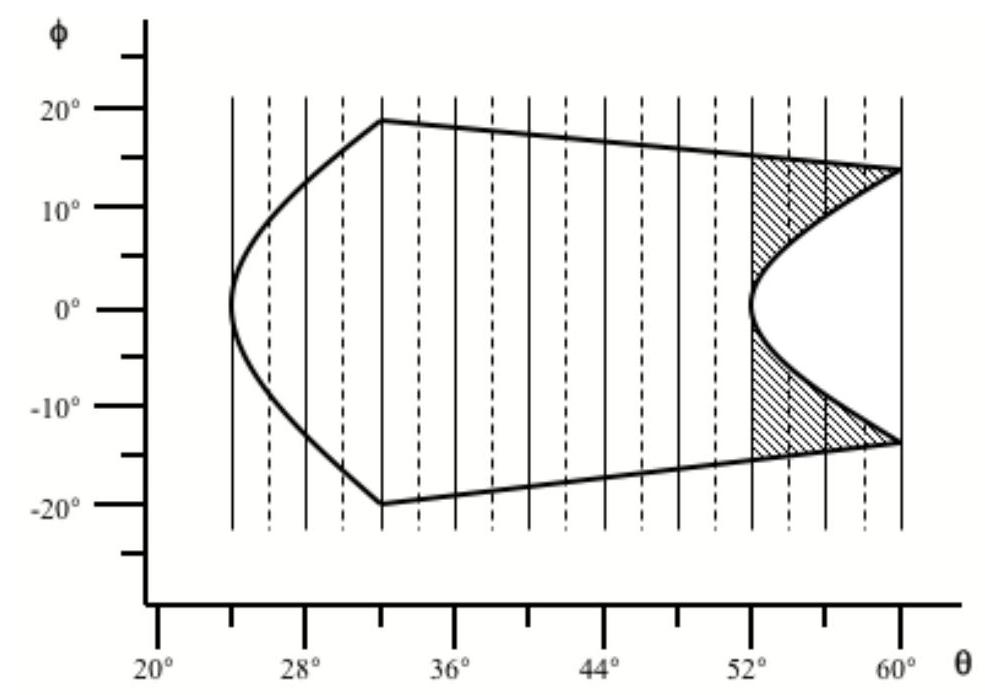
\includegraphics[max width=\textwidth, center]{2025_02_07_204a351db2d7f48b61ebg-139}

Figure 7.1: A rectangular particle detector has a non-azimuthally symmetric shape in the $\theta, \phi$ space of projectile scattering angle. This shape must be defined by entering a number ( $N F I$ ) of azimuthal angular ranges. In the hatched region, $N F I=2$ ranges must be entered specifying the two active regions. The solid lines represent $\theta$ meshpoints, while the dashed lines indicate $\theta$ subdivisions. The rapid variation in active $\phi$ range in the hatched region necessitates input of the active ranges of $\Delta \phi$ at each subdivision specifying each of the two active detection regions shown hatched.\\
$\mathbf{N I} 1, \pm \mathbf{N I} 2 \quad$ The number of equal subdivisions of energy ( $N I 1$ ) and projectile scattering angle (NI2) used for integration. $N I 1 \leq 100,|N I 2| \leq 100$. If SPL, is selected on the CONT suboption, then the cubic spline interpolation subroutines SPLINE, SPLINT [PRE92] are used to interpolate between the $\left(E_{i}, \theta_{i}\right)$ meshpoints at which the full Coulomb excitation calculations of the deexcitation $\gamma$-ray yields were performed (See Section 6.5). The rapid angle dependence of the Rutherford scattering cross section at forward angles can cause problems with interpolation for the elastic channel if insufficient angle subdivisions are used. Always use many integration subdivisions which has little impact on the speed of the program since the full Coulomb excitation calculations are performed only at the meshpoints, not at the intergration points, and interpolation is fast. NI1 should be even and not exceed 100 while NI2 must not exceed 100. If odd values are given the program increases them to the next larger even number. However, the $\Delta \phi$ input will be confused if $N I 2$ is negative and odd. Important: NI2 can be negative and must be negative if $N T$ is specified to be negative. Conversely, $N I 2$ must be positive if $N T$ is positive. If $N I 2$ is negative then the following input must be provided:\\
$\Delta \phi_{1}, \Delta \phi_{2}, \ldots \boldsymbol{\Delta} \phi_{|N I 2|+1} \quad$ where $\Delta \phi_{i}$ is the total range of $\phi$ (in degrees) for each equal subdivision of projectile scattering angle as illustrated in Figure 7.1. That is, $\Delta \phi_{i}$ equals the sum of all $\phi$ ranges for a given subdivision $\theta$ value if the azimuthal angular range also is subdivided into non-contiguous regions. The $\Delta \phi$ values correspond to equal divisions of projectile scattering angle from $\theta_{\min }$ to $\theta_{\max }$ rather than equal subdivisions of the meshpoints as in the normal input for NI2 $>0$. Note that there is an important difference in how the interpolation over scattering angle is performed depending on whether $N T$ and $N I 2$ are both positive or both negative. For the positive sign the program interpolates between the calculated yields at each $\theta$ meshpoint. This produces excellent results if the $\phi$ dependence of the particle detector is a smooth function of projectile scattering angle, $\theta$. The negative sign option should be used if the $\phi$ dependence is more complicated or if $\phi$ changes rapidly with $\theta$. When the negative sign is used the program stores for each meshpoint the calculated yields per unit angle of azimuthal range, i.e., the calculated yields divided by the total $\phi$ range specified at thatangle for the exact calculation. The program then interpolates these yields per unit of $\phi$ between the meshpoints. These interpolated values then are multiplied by the appropriate $\Delta \phi$ for each subdivision meshpoint prior to integration. Note that the code uses NI2 equal subdivisions of projectile scattering angles. This is not the same\\
as equal division of geometric angle of the detector if the recoiling target nucleus is detected.\\
The following sample input segment goes with Figure 7.1. It shows the input of the absolute azimuthal angles under NFI, which are entered if the azimuthal symmetry flag was turned off in sub-option EXPT.\\
It also shows the entry of total azimuthal angular ranges when NT and NI2 are set to negative values.

\begin{verbatim}
OP,INTG
5,-10,634,650,24.0,60.0
634,638,642,646,650
24.,28.,32.,36.,40.,44.,48.,52.,56.,60.
1
1
1
-12.5,12.5
1
-18.75,18.75
1
-18.0,18.0
1
-17.5,17.5
1
-17.0,17.0
1
-16.0,16.0
2
-15.0,-2.0,2.0,15.0
2
-14.5,-9.0,9.0,14.5
2
-13.75,-13.0, 13.0,13.75
4
4
32.395,32.401,32.404,32.404
10,-18
NP
E
NE,NT,E E min},\mp@subsup{\textrm{E}}{\operatorname{max}}{},\mp@subsup{0}{\operatorname{min}}{},\mp@subsup{0}{\mathrm{ max }}{
E
NFI
\phi
NFI
\phi}\mp@subsup{}{1}{}\mp@subsup{\phi}{2}{
etc.
4. ,16.25,24.5,31.25,37.5,36.9,36.25,35.6,35,34.1,33.25,
32.6,31.9,29.2,26.5,18.5,11.2,5.7,1.5
\end{verbatim}

The last two lines contain the $N I 2+1=19$ values of $\Delta \phi$ for $\theta=20.0^{\circ}$ to $60.0^{\circ}$. These correspond to the $\theta$ values $20.0^{\circ}, 22.0^{\circ}, 24 .^{\circ}, \ldots$ in Figure 7.1.

The circular detector option (CONT CRD,) incorporates a feature to calculate automatically the azimuthal angular range $\Delta \phi$ at each subdivision of scattering angle $\theta$. Consequently, do not input $\Delta \phi$ values when using the circular detector option.

The integration-related portion of the input must be repeated for each experiment defined in suboption EXPT.

It is recommended to use as small a number of meshpoints as possible because the full Coulomb excitation calculations performed at the meshpoints are time-consuming. In many cases the required accuracy can be achieved by requesting a large number of subdivisions between the meshpoints, the values in subdivision points being found by fast interpolation.

\section*{Circular detector option}
The input for a given experiment differs slightly if the circular detector option is selected. This option is activated by the flag CRD, in the CONT suboption of either OP, COUL or OP,GOSI. For such experiments the input to OP,INTG is as follows:\\
$\mathbf{N E}, \mathbf{N T}, \mathbf{E}_{\text {min }}, \mathbf{E}_{\text {max }}, \boldsymbol{\theta}, \boldsymbol{\phi}, \boldsymbol{\theta}_{1 / 2} \quad$ In this case $\theta$ and $\phi$ are the angular coordinates of the center of a circular particle detector subtending the half-angle $\theta_{1 / 2}$. The remaining entries are identical to the ones described in the previous section.\\
$\mathbf{E}_{1}, \mathbf{E}_{2}, \ldots, \mathbf{E}_{N E} \quad$ The energy meshpoints for the full Coulomb excitation calculation, analogous to those described in the previous section.

The above input is used in the first stage, that is, in the meshpoint calculation. When using arrays of PIN diodes follow the instructions described in the instructions in CONT; switch PIN. The input of the second stage, that is, the integration section, should look as follows:

NP Number of stopping powers to be input.\\
$\mathbf{E}_{1}, \mathbf{E}_{2}, \ldots, \mathbf{E}_{N P} \quad$ Energy meshpoints for the stopping powers in MeV .\\
$(d E / d x)_{1}, \ldots,(d E / d x)_{N P}$ The values of the stopping powers, analogous to the normal input. If $N P=0$ the values of this table will be those from the previous experiment.

NI1, NI2 Number of subdivisions of energy (NI1) and projectile scattering angle (NI2) used during the integration. Both shall be even numbers and shall not exceed 100 and 50 respectively.

Although OP,INTG has been deprecated in favour of OP,INTI, the following example illustrates a case where OP,INTG still can be of use. An inverse kinematics experiment is performed and one of the two kinematic solutions is separated in the data acquisition. In order to correctly compare the predicted yields with the measured yields, the OP,CORR and OP,INTG/INTI steps must correctly separate the measured solution as well. If the p-gamma data are then separated in the sorting into two or more particle scattering ranges, then more sensitivity in fitting is obtained by normalizing these Gosia "logical" experiments together. See the EXPT section. The user will then have to use the original OP,INTG option, paying attention to the accuracy of defining the cutoff angle (section 6.5.2). This is because separation of the two kinematic solutions with OP,INTI is accomplished by selecting the target recoil as the detected particle and setting the recoil angle limits to choose either the forward or backward center of mass solution. As noted in section 7.32, logical experiments that specify recoil detection must be normalized independently in the present version of Gosia. If the cutoff angle cannot be defined accurately enough to obtain the desired accuracy in the calculations, then the alternative is to use OP,INTI and commit to some loss of sensitivity in the fitting, but with greater accuracy. The loss of sensitivity may or may not be problematic, depending on the quantity and precision of spectroscopic data in the fit (section OP,YIEL).

\section*{Summary of input to OP,INTG - Normal input}
\section*{OP,INTG}
$$
\begin{aligned}
& N E, N T, E_{\min }, E_{\max }, \theta_{\min }, \theta_{\max } \\
& E_{1}, E_{2}, \ldots, E_{N E} \\
& \pm \theta_{1}, \pm \theta_{2}, \ldots, \pm \theta_{N T}
\end{aligned}
$$

NFI\\
$\phi_{1}, \phi_{2}, \ldots, \phi_{2 N F I-1}, \phi_{2 N F I}$\\
This portion of input is to be entered for each experiment defined in EXPT, unless the axial symmetry or circular detector option have been used.

$$
\begin{aligned}
& N P \\
& E_{1}, E_{2}, \ldots, E_{N P} \\
& (d E / d x)_{1},(d E / d x)_{2}, \ldots,(d E / d x)_{N P}
\end{aligned}
$$

$N I 1, \pm N I 2$\\
$\Delta \phi_{1}, \Delta \phi_{2}, \ldots, \Delta \phi_{|N I 2|+1}$

This portion of the input again must be given for each experiment.

\section*{Summary of input to OP,INTG - Circular detector option}
OP,INTG\\
$N E, N T, E_{\text {min }}, E_{\text {max }}, \theta, \phi, \theta_{1 / 2}$\\
$E_{1}, E_{2}, \ldots, E_{N E}$

This input should be defined in the part of the input related to the calculation of the meshpoints. The remainder, listed below, should be included in the integration-related section.

$$
\begin{aligned}
& N P \\
& E_{1}, E_{2}, \ldots, E_{N P} \\
& (d E / d x)_{1},(d E / d x)_{2}, \ldots,(d E / d x)_{N P} \\
& N I 1, N I 2
\end{aligned}
$$

\subsection*{7.12.1 Calculation of observables:}
Chapter 6.6 gives the equations needed to evaluate typical observables using the Gosia output. For convenience the basic equations are reprinted here.

\section*{Absolute coincident $p-\gamma$ yields}
Note that OP.INTG evaluates the integrated coincident $\gamma$-ray yield for transition $I \rightarrow I_{f}$ that is defined by equations 6.35--6.44.

Integrating the angle-integrated yields through the thickness of the target gives the total integrated yield $Y_{i}\left(I \rightarrow I_{f}\right)$ are given by equation $6.44 b$. These are the $\gamma$-ray yields that are fit to the experimental yields. Note that $Y\left(I \rightarrow I_{f}\right)$ includes the Rutherford cross section, the $\sin \left(\theta_{p}\right)$ term, the target thickness, integration over the $\theta_{p}, \phi_{p}$ for the detected coincident particles, the deorientation effect and $\gamma$-detector $Q_{K}$ attenuation coefficients. OP,INTG does not include the detection efficiencies per unit solid angle for charged particle and $\gamma$-rays, $\varepsilon_{p}$ and $\varepsilon_{\gamma}$. The units for both the integrated coincident $p-\gamma$-ray yields and the integrated Rutherford $p$ singles yields are $m b \cdot\left(\mathrm{mg} / \mathrm{cm}^{2}\right) / s r$ where the $1 / s r$ term is for the solid angle of the $\gamma$-ray detector $\Delta \Omega_{\gamma}$

The total number of coincident $\gamma$-rays detected then is given by\\
Detected $p-\gamma$ coincident events $N_{i}=10^{-30} \cdot\left[\frac{Q}{\hat{q} e}\right] \cdot\left[\frac{N_{A}}{A}\right] \cdot Y\left(I \rightarrow I_{f}\right) \cdot \varepsilon_{p} \cdot \varkappa_{p \gamma} \cdot \varepsilon_{\gamma}\left(E_{\gamma}\right) \cdot \Delta \Omega_{\gamma}$\\
where:\\
$Q \quad$ is the integrated beam charge in Coulombs $[C]$\\
$\hat{q} \quad$ the average charge state of the beam\\
$e \quad$ the proton charge $\left[1.602 \times 10^{-19} C\right]$\\
$N_{A} \quad$ Avogadro number $\left(6.022 \times 10^{23}\right.$ Atoms $\left./ \mathrm{mol}\right)$\\
$A$ target mass number $(\mathrm{gm} / \mathrm{mol})$\\
$\frac{d E}{d x} \quad$ energy loss in target in $\left[\frac{\mathrm{MeV}}{\mathrm{mg} / \mathrm{cm}^{2}}\right]$\\
$Y\left(I \rightarrow I_{f}\right) \quad$ is the angle and beam-energy integrated OP.INTG output in $\left[\mathrm{mb} \cdot \mathrm{mg} / \mathrm{cm}^{2} / \mathrm{sr}\right]$\\
$\varepsilon_{p} \quad$ particle detection efficiency per unit solid angle. Typically this is $\varepsilon_{p}=1$ regardless of solid angle covered by the integration in OP,INTG or OP.INTI.\\
$\varepsilon_{\gamma}\left(E_{\gamma}\right) \quad$ the energy dependent $\gamma$-ray peak detection efficiency per unit solid angle $\Delta \Omega_{\gamma}$. This would be, $\varepsilon_{\gamma}=1$ for a perfect blackbody $\gamma$-ray detector. Note that the efficiency $\varepsilon_{\gamma}\left(E_{\gamma}\right)$ must be evaluated at the observed Doppler-shifted $\gamma$-ray energy $E_{\gamma}$ when the photons are emitted in flight.\\
$\Delta \Omega_{\gamma}$ is the solid angle subtended by the $\gamma$-ray detector. Read chapter 6.6.1 for a discussion of the product $\varepsilon_{\gamma}\left(E_{\gamma}\right) \cdot \Delta \Omega_{\gamma}$.\\
$\varkappa_{p \gamma} \quad$ the $p-\gamma$ live time efficiency factor to account for the fraction of the time for which the dataacquisition system is dead due to system dead time, or pileup rejection.

Examples of the calculation of the absolute counts are given in chapter 6.6.1.\\
$p-\gamma$ yields normalized to the scattered "Singles" particle yields\\
For many experiments the observable is the ratio of the absolute integrated $p-\gamma$ coincidence yields normalized to the "singles" particle scattering yield detected using the same particle detector as used for detecting the $p-\gamma$ events. Typically the energy resolution for the particle detector is insufficient to resolve the elastic peak from the individual low-lying excited states. Thus the observed "singles" yield is the sum over all excited states.

The " $p$ singles" yield for absolute normalization of the $p-\gamma$ coincidence yields is given by 6.70. The units of $Y_{\text {Si } n g l e s}$ are $\left[\mathrm{mb} \cdot \mathrm{mg} / \mathrm{cm}^{2}\right]$.

The total number of elastically scattered events detected is given by


\begin{equation*}
\text { Detected } p \text { singles events }=N_{\text {Si } n g l e s}=10^{-30} \cdot\left[\frac{Q}{\hat{q} e}\right] \cdot\left[\frac{N_{A}}{A}\right] \cdot Y_{\operatorname{Si} n g l e s} \cdot \varepsilon_{p} \cdot \varkappa_{p} \tag{6.70}
\end{equation*}


The terms in this equation are the same as those defined in equation 6.65\\
If the observable is the ratio of $p-\gamma$ coincidences normalized to particle singles, this can be computed by the ratio


\begin{equation*}
\frac{\text { Detected } p-\gamma \text { coincident events }}{\text { Detected } p \text { singles events }}=\frac{N_{i}}{N_{\text {Si ngles }}}=\frac{Y\left(I \rightarrow I_{f}\right)}{Y_{\text {Si } n g l e s}} \cdot \frac{\varkappa_{p \gamma}}{\varkappa_{p}} \cdot \varepsilon_{\gamma}\left(E_{\gamma}\right) \cdot \Delta \Omega_{\gamma} \tag{7.1}
\end{equation*}


For the ratio the total beam and target thickness factors in equations 6.65 and 6.70 cancel. There remain two important factors needed to use the $p-\gamma$ yields normalized to the scattered singles particle yields in order to measure the ratio of the $p-\gamma$ cross section to particle singles cross section . The first factor is the ratio of the $p-\gamma$ lifetime efficiency $\varkappa_{p \gamma}$ to the $p$ singles lifetime efficiency $\varkappa_{p}$. If both the $p-\gamma$ and $p$ singles events are not prescaled then $\frac{\varkappa_{p \gamma}}{\varkappa_{p}} \approx 1$. However, since the singles count rate typically is 100 to 1000 time higher than the $p-\gamma$ rate it is usually to prescale the singles events by factors of 100 to 1000 to reduce the fraction of singles events. The time interval between individual singles counts is random. Prescaling derandomizes the time between the prescaled single events causing them to occur at quasi-regular time intervals. This derandomizing can lead to zero effective dead time for recording prescaled single events in contrast to the deadtime losses for the $p-\gamma$ coincident events. As consequence the livetime ratio $\frac{\varkappa_{p \gamma}}{\varkappa_{p}}<1$. Care must be taken to measure or calculate the livetime ratio $\frac{\varkappa_{p \gamma}}{\varkappa_{p}}$. The other factor that is needed to derive the absolute $p-\gamma$ cross sections from the relative yields is the total $\gamma$-ray detection efficiency $\varepsilon_{\gamma}\left(E_{\gamma}\right) \cdot \Delta \Omega_{\gamma}$. As mentioned above, the factor $\varepsilon_{\gamma}\left(E_{\gamma}\right) \cdot \Delta \Omega_{\gamma}$ must include the $p-\gamma$ time gating efficiency as well as the total $\gamma$-ray peak detection efficiency.

Note that Gosia does not directly fit to the ratio $\frac{\text { Detected } p-\gamma \text { coincident events }}{\text { Detected } p \text { singles events }}$, but such a fit can be acheived by ensuring that the independent Gosia calculations of the $p-\gamma$ coincident event and the $p$ singles yields have a common normalization constant.

\section*{Relative target and projectile $p-\gamma$ yields observed in a single experiment}
A frequent observable involves measurement of the ration of target and projectile $p-\gamma$ yields from one experiment where both target and projectile Coulomb excitation occur. This type of measurement has the advantage that many terms in equation 6.65 cancel. The ratio of the projectile and target $p-\gamma$ yields is given by.


\begin{equation*}
\frac{\text { Detected projectile } p-\gamma \text { coincident events }}{\text { Detected target } p-\gamma \text { coincident events }}=\frac{N_{i}^{P}}{N_{k}^{T}}=\frac{Y^{P}\left(I_{i}^{p} \rightarrow I_{f}^{P}\right)}{Y^{T}\left(I_{i}^{T} \rightarrow I_{f}^{T}\right)} \cdot \frac{\varepsilon_{\gamma}\left(E_{\gamma}^{P}\right)}{\varepsilon_{\gamma}\left(E_{\gamma}^{T}\right)} \tag{7.2}
\end{equation*}


The only additional factor needed to convert the Gosia output to determine the observable is the ratio $\frac{\varepsilon_{\gamma}\left(E_{\gamma}^{P}\right)}{\varepsilon_{\gamma}\left(E_{\gamma}^{T}\right)}$. As discussed in chapter 4.6 the symmetry axis of the angular distribution is identical for either target or projectile excitation. However, the Doppler shift is quite different for target and projectile in-flight $\gamma$-ray emission because of the different recoil directions and velocities of the emitting projectile and target. The ratio of target and projectile $p-\gamma$ yields can be performed using Gosia by ensuring that the independent Gosia calculations for target and projectile excitation have a common normalization constant.

The special code GOSIA2, described in chapter 11, is specifically designed to handle the common normalization occuring for such experiments, This helps the analysis when performing Coulomb excitation that use weak intensity beams for which very few transitions are observed in either target or projectile excitation. Further details can be found in chapter 11.

\subsection*{7.13 OP,INTI (INTEGRATE-2008)}
The integrate command produces the most accurate calculation of the yields of deexcitation $\gamma$-rays following Coulomb excitation to be used for realistic comparison with experimental data. This option includes integration over solid angle of the particle detectors, energy loss in the target as well as full correction for the recoil velocity of the deexciting nucleus and the deorientation effect. This option also integrates the Rutherford scattering over the particle detectors and energy loss in the target which can be used as an absolute normalization.

The 1980 version of the integration code, OP,INTG has been superceded by the integration code, OP,INTI, which was developed by Nigel Warr in 2008 to handle a problem that occurs for integration of systems involving inverse kinematics when the recoiling target nucleus is detected. This problem and the solution are described in chapter 6.5.2. The OP,INTG and OP,INTI inputs are identical except that the angles of the detected particle are always used as input for OP,INTI. This distinction is of consequence when the detected particle is the recoiling target nucleus rather than the scattered projectile. The $\theta$ meshpoints in OP,INTI are specified by laboratory angles of the detected particle in contrast to OP,INTG where the scattered projectile angles are used. A subroutine INVKIN uses the angle of the recoiling target nucleus to calculate the the corresponding angle of the scattered projectile which is then used by GOSIA. For target detection the IKIN input in EXPT is ignored by OP,INTI and this flag is set internally. Note that as described in section 6.5.2 projectile recoil detection for inverse kinematics requires running the Gosia calculation twice, once with $\operatorname{IKIN}=0$ and once with $\operatorname{IKIN}=1$ and then manually summing the calculated yields. The option OP,INTI always should be used when running GOSIA. The option OP,INTG remains for running legacy GOSIA inputs or for some inverse kinematics cases where normalization is needed.

OP,INTI comprises two distinct stages. The first stage calculates the yields of deexcitation $\gamma$-rays integrated over azimuthal angle $\phi$ for each energy and detected particle scattering angle meshpoint. This calculation of the meshpoint yields should be repeated for each experiment according to the order that the experiments appear in the EXPT input. GOSIA stores the calculated meshpoint yields as internal files. The second stage uses the data stored in these internal files to integrate over bombarding energy and the range of scattering angles subtended by the particle detectors which is performed by interpolating between the $\gamma$ yields calculated at each meshpoint. It is permitted to integrate over any arbitrary $(\theta, \phi)$ shape for the particle detector including the case of several $(\leq 4) \phi$ ranges for each $\theta$ value. An option is included to simplify integration over circular detectors because of the frequent use of such a geometry. The input for the circular detector is a slightly modified subset of the normal input.

It is strongly recommended that the $S P L, X$. option in CONT be set to\\
SPL, 1.\\
in order to select use of the cubic spline interpolation procedure. For more than 20 mesh points the Lagrange interpolation approach is unreliable since it diverges.

Note that $O P, G O S I$, including its four suboptions, plus $O P, Y I E L$, must occur in the input file prior to $O P, I N T I$ in order to provide the input necessary to run $O P, I N T I$.

The full input to OP,INTI is described below followed by the input for the circular detector option. Since the input to OP,INTI is long, a summary of the input is given at the end of this section to serve as a quick reference. Section 14.3 shows the correct location of OP,INTI in the input stream.

\section*{Normal input to OP,INTI}
The input sequence is as follows:

\section*{OP,INTI}
$\mathrm{NE}, \pm \mathbf{N T}, \mathbf{E}_{\text {min }}, \mathbf{E}_{\text {max }}, \boldsymbol{\theta}_{\text {min }}, \boldsymbol{\theta}_{\max }$\\
where:\\
NE The total number of energy meshpoints at which full Coulomb excitation calculations will be performed $(N E \leq 100)$.

NT The total number of $\theta$ meshpoints at which the full Coulomb excitation calculations will be performed, $(N T \leq 100)$. Negative value of $N T$ specifies that the $\Delta \phi$ data specifying the shape of the detector will be entered by the user to improve the accuracy for complicated $\theta, \phi$, shapes. ( see below)\\
$\mathbf{E}_{\min }, \mathbf{E}_{\max } \quad$ The minimum and maximum bombarding energies (in MeV ) between which the integration is to be performed.\\
$\boldsymbol{\theta}_{\min }, \boldsymbol{\theta}_{\max } \quad$ The minimum and maximum angles (in degrees) between which the integration is to be performed. Note, $\theta$ angles are always positive, with $\theta_{\max }>\theta_{\min }$ and correspond to laboratory scattering angles of the detected particle, that is, the angle of the scattered projectile if it is detected and the angle of the recoiling target nucleus if it is detected. Note that the recoil angle is very sensitive to the kinematic Q-value assumed for small angle scattering of light nuclei on a heavy target. The above input string is modified if the circular detector flag CRD in CONT is activated for this experiment, as described later.\\
$\mathbf{E}_{1}, \mathbf{E}_{2}, \ldots \mathbf{E}_{N E} \quad$ Energy meshpoints at which the exact Coulomb excitation calculations are performed (MeV). These must exceed or at least equal the range over which the integration is to be performed to obtain reliable spline interpolation.\\
$\boldsymbol{\theta}_{1}, \boldsymbol{\theta}_{2}, \ldots \boldsymbol{\theta}_{N T} \quad$ Detected scattering angles (degrees) in the laboratory frame, input in increasing order, are used as meshpoints to define the $\phi$ angular shape of the particle detector boundaries. The input angles must correspond to the detected particle angular range which exceeds or at least equals the range of angles subtended by the detector to obtain reliable spline interpolation. Do not input these angles for the circular detector option.

NFI The number of $\phi$ ranges for each $\theta_{i}$ meshpoint needed to describe the $\theta(\phi)$ dependence. Omit $N F I$ input if either the circular detector option or axial symmetry is specified.\\
$\phi_{1}, \phi_{2}, \ldots \quad N F I$ pairs of $\phi$ angles (degrees) describing the $\phi$ range for given $\theta_{i}$. Omit $\phi$ input if either the circular detector option or axial symmetry is specified.

The above two records must be input for each $\theta$ meshpoint specified. NFI should not exceed 4. In most cases $N F I=1$, then the pair of $\phi$ angles simply specifies the lower and upper flimits for a given $\theta$ meshpoint. However, for some geometries, such as for rectangular shaped detectors, it is necessary to include more than one $\phi$ range for some $\theta$ values. For example, a rectangular detector placed with its normal at $45^{\circ}$ to the incident beam has $(\theta, \phi)$ contours shown in Figure 7.2:

This ends the input required to calculate the $\gamma$-ray yields integrated over azimuthal angle $\phi$ at the specified set of meshpoints. This part of input must be repeated for all experiments defined in EXPT.

The second stage of the input is required for the integration and once again has to be entered for all experiments:

NP Number of stopping powers to be input, $3 \leq N P \leq 20$. If $N P=0$ then the stopping power table is taken from the previous experiment and the following input of energy and $d E / d x$ values can be omitted for this case. This is useful where experiments differ only with regard to range of scattering angles or bombarding energies.\\
$\mathbf{E}_{1}, \mathbf{E}_{2}, \ldots \mathbf{E}_{N P} \quad$ The energy meshpoints (in MeV ) at which values of the stopping power are to be input.\\
$\left(\frac{d E}{d x}\right)_{1} . .\left(\frac{d E}{d x}\right)_{N P} \quad$ Stopping powers in units of $\mathrm{MeV} /\left(\mathrm{mg} / \mathrm{cm}^{2}\right)$. Interpolation between the energy meshpoints of the stopping power table is performed during integration. Consequently it is important to ensure that the range of energy meshpoints of the stopping power table exceed the range of energies over which the integration is to be performed. As discussed in chapter 5.3 , it is strongly recommended that the code Ziegler[ZIE08] SRIM be employed to generate the stopping powers.\\
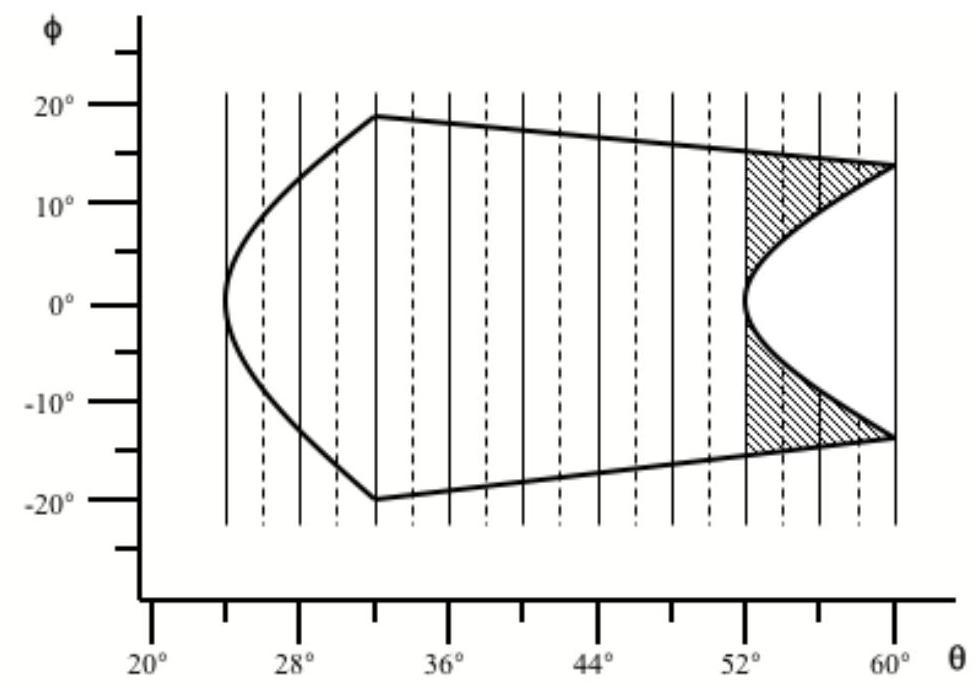
\includegraphics[max width=\textwidth, center]{2025_02_07_204a351db2d7f48b61ebg-147}

Figure 7.2: A rectangular particle detector has a non-azimuthally symmetric shape in the $\theta, \phi$ space of projectile scattering angle. This shape must be defined by entering a number ( $N F I$ ) of azimuthal angular ranges. In the hatched region, $N F I=2$ ranges must be entered specifying the two active regions. The solid lines represent $\theta$ meshpoints, while the dashed lines indicate $\theta$ subdivisions. The rapid variation in active $\phi$ range in the hatched region necessitates input of the active ranges of $\Delta \phi$ at each subdivision specifying each of the two active detection regions shown hatched.\\
$\mathbf{N I} 1, \pm \mathbf{N I} 2 \quad$ The number of equal subdivisions of energy ( $N I 1$ ) and detected particle scattering angle (NI2) used for integration. $N I 1 \leq 100,|N I 2| \leq 100$. The cubic spline interpolation subroutines SPLINE, SPLINT [PRE92] are used to interpolate between the $\left(E_{i}, \theta_{i}\right)$ meshpoints at which the full Coulomb excitation calculations of the deexcitation $\gamma$-ray yields were performed (See Section 6.5.2). The rapid angle dependence of the Rutherford scattering cross section at forward angles can cause problems with interpolation for the elastic channel if insufficient angle meshpoints are used. Always use many integration subdivisions which has little impact on the speed of the program since the full Coulomb excitation calculations are performed only at the meshpoints, not at the intergration points, and interpolation is fast. NI1 should be even and not exceed 100 while NI2 must not exceed 100. If odd values are given the program increases them to the next larger even number. However, the $\Delta \phi$ input will be confused if NI2 is negative and odd. Important: NI2 can be negative and must be negative if $N T$ is specified to be negative. Conversely, $N I 2$ must be positive if $N T$ is positive. If $N I 2$ is negative then the following input must be provided:\\
$\Delta \phi_{1}, \Delta \phi_{2}, \ldots \Delta \phi_{|N I 2|+1} \quad$ where $\Delta \phi_{i}$ is the total range of $\phi$ (in degrees) for each equal subdivision of projectile scattering angle as illustrated in Figure 7.2. That is, $\Delta \phi_{i}$ equals the sum of all $\phi$ ranges for a given subdivision $\theta$ value if the azimuthal angular range also is subdivided into non-contiguous regions. The $\Delta \phi$ values correspond to equal divisions of projectile scattering angle from $\theta_{\min }$ to $\theta_{\max }$ rather than equal subdivisions of the meshpoints as in the normal input for NI2 $>0$. Note that there is an important difference in how the interpolation over scattering angle is performed depending on whether $N T$ and $N I 2$ are both positive or both negative. For the positive sign the program interpolates between the calculated yields at each $\theta$ meshpoint. This produces excellent results if the $\phi$ dependence of the particle detector is a smooth function of projectile scattering angle, $\theta$. The negative sign option should be used if the $\phi$ dependence is more complicated or if $\phi$ changes rapidly with $\theta$. When the negative sign is used the program stores for each meshpoint the calculated yields per unit angle of azimuthal range, i.e., the calculated yields divided by the total $\phi$ range specified at that angle for the exact calculation. The program then interpolates these yields per unit of $\phi$ between the meshpoints. These interpolated values then are multiplied by the appropriate $\Delta \phi$ for each subdivision meshpoint prior to integration. Note that the code uses NI2 equal subdivisions of detected particle scattering angles.

The following sample input segment goes with Figure 7.2. It shows the input of the absolute azimuthal angles under NFI, which are entered if the azimuthal symmetry flag was turned off in sub-option EXPT.\\
It also shows the entry of total azimuthal angular ranges when NT and NI2 are set to negative values.

\begin{verbatim}
OP,INTI
5,-10,634,650,24.0,60.0
634,638,642,646,650
24.,28.,32.,36.,40.,44.,48.,52.,56.,60.
1
-2.0,2.0
1
-12.5,12.5
1
-18.75,18.75 etc.
1
-18.0,18.0
1
-17.5,17.5
1
-17.0,17.0
1
-16.0,16.0
2
-15.0,-2.0,2.0,15.0
2
-14.5,-9.0,9.0,14.5
2
-13.75,-13.0,13.0,13.75
4
4
32.395,32.401,32.404,32.404
10,-18
4 NP
NE,NT,E Emin},\mp@subsup{\textrm{E}}{\mathrm{ max }}{},\mp@subsup{0}{min}{m},\mp@subsup{0}{\mathrm{ max }}{
E
NFI
\phi}\mp@subsup{|}{1}{}\mp@subsup{\phi}{2}{
NFI
\phi
4.,16.25,24.5,31.25,37.5,36.9,36.25,35.6,35,34.1,33.25,
32.6,31.9,29.2,26.5,18.5,11.2,5.7,1.5
\end{verbatim}

The last two lines contain the $N I 2+1=19$ values of $\Delta \phi$ for $\theta=20.0^{\circ}$ to $60.0^{\circ}$. These correspond to the $\theta$ values $20.0^{\circ}, 22.0^{\circ}, 24 .^{\circ}, \ldots$ in Figure 7.2.

The circular detector option (CONT CRD,) incorporates a feature to calculate automatically the azimuthal angular range $\Delta \phi$ at each subdivision of scattering angle $\theta$. Consequently, do not input $\Delta \phi$ values when using the circular detector option.

The integration-related portion of the input must be repeated for each experiment defined in suboption EXPT.

It is recommended to use as small a number of meshpoints as possible because the full Coulomb excitation calculations performed at the meshpoints are time-consuming. In many cases the required accuracy can be achieved by requesting a large number of subdivisions between the meshpoints, the values in subdivision points being found by fast interpolation.

\section*{Circular detector option}
The input for a given experiment differs slightly if the circular detector option is selected. This option is activated by the flag CRD, in the CONT suboption of either OP, COUL or OP,GOSI. For such experiments the input to OP,INTI is as follows:\\
$\mathbf{N E}, \mathbf{N T}, \mathbf{E}_{\text {min }}, \mathbf{E}_{\text {max }}, \boldsymbol{\theta}, \boldsymbol{\phi}, \boldsymbol{\theta}_{1 / 2} \quad$ In this case $\theta$ and $\phi$ are the angular coordinates of the center of a circular particle detector subtending the half-angle $\theta_{1 / 2}$. The remaining entries are identical to the ones described in the previous section.\\
$\mathbf{E}_{1}, \mathbf{E}_{2}, \ldots, \mathbf{E}_{N E} \quad$ The energy meshpoints for the full Coulomb excitation calculation, analogous to those described in the previous section.

The above input is used in the first stage, that is, in the meshpoint calculation. When using arrays of PIN diodes follow the instructions described in the instructions in CONT; switch PIN.

The input of the second stage, that is, the integration section, should look as follows:\\
NP Number of stopping powers to be input.\\
$\mathbf{E}_{1}, \mathbf{E}_{2}, \ldots, \mathbf{E}_{N P} \quad$ Energy meshpoints for the stopping powers in MeV.\\
$(d E / d x)_{1}, \ldots,(d E / d x)_{N P}$ The values of the stopping powers, analogous to the normal input. If $N P=0$ the values of this table will be those from the previous experiment.

NI1, NI2 Number of subdivisions of energy (NI1) and projectile scattering angle (NI2) used during the integration. Both shall be even numbers and shall not exceed 100 and 50 respectively.

\section*{Summary of input to OP,INTI - Normal input}
OP,INTI\\
$N E, N T, E_{\min }, E_{\max }, \theta_{\min }, \theta_{\max }$\\
$E_{1}, E_{2}, \ldots, E_{N E}$\\
$\pm \theta_{1}, \pm \theta_{2}, \ldots, \pm \theta_{N T}$\\
NFI\\
$\phi_{1}, \phi_{2}, \ldots, \phi_{2 N F I-1}, \phi_{2 N F I}$\\
This portion of input is to be entered for each experiment defined in EXPT, unless the axial symmetry or circular detector option have been used.

$$
\begin{aligned}
& N P \\
& E_{1}, E_{2}, \ldots, E_{N P} \\
& (d E / d x)_{1},(d E / d x)_{2}, \ldots,(d E / d x)_{N P} \\
& N I 1, \pm N I 2 \\
& \Delta \phi_{1}, \Delta \phi_{2}, \ldots, \Delta \phi_{|N I 2|+1}
\end{aligned}
$$

This portion of the input again must be given for each experiment.

\section*{Summary of input to OP,INTI - Circular detector option}
\section*{OP,INTI}
$$
\begin{aligned}
& N E, N T, E_{\min }, E_{\max }, \theta, \phi, \theta_{1 / 2} \\
& E_{1}, E_{2}, \ldots, E_{N E}
\end{aligned}
$$

This input should be defined in the part of the input related to the calculation of the meshpoints. The remainder, listed below, should be included in the integration-related section.

$$
\begin{aligned}
& N P \\
& E_{1}, E_{2}, \ldots, E_{N P} \\
& (d E / d x)_{1},(d E / d x)_{2}, \ldots,(d E / d x)_{N P} \\
& N I 1, N I 2
\end{aligned}
$$

\subsection*{7.13.1 Calculation of observables:}
Chapter 6.6 gives the equations needed to evaluate typical observables using the Gosia output. For convenience the basic equations are reprinted here.

\section*{Absolute coincident $p-\gamma$ yields}
Note that OP.INTI evaluates the integrated coincident $\gamma$-ray yield for transition $I \rightarrow I_{f}$ that is defined by equations 6.35--6.44.

Integrating the angle-integrated yields through the thickness of the target gives the total integrated yield $Y_{i}\left(I \rightarrow I_{f}\right)$ are given by equation $6.44 b$. These are the $\gamma$-ray yields that are fit to the experimental yields. Note that $Y\left(I \rightarrow I_{f}\right)$ includes the Rutherford cross section, the $\sin \left(\theta_{p}\right)$ term, the target thickness, integration over the $\theta_{p}, \phi_{p}$ for the detected coincident particles, the deorientation effect and $\gamma$-detector $Q_{K}$ attenuation coefficients. OP,INTI does not include the detection efficiencies per unit solid angle for charged particle and $\gamma$-rays, $\varepsilon_{p}$ and $\varepsilon_{\gamma}$. The units for both the integrated coincident $p-\gamma$-ray yields and the integrated Rutherford $p$ singles yields are $m b \cdot\left(\mathrm{mg} / \mathrm{cm}^{2}\right) / \mathrm{sr}$ where the $1 / \mathrm{sr}$ term is for the solid angle of the $\gamma$-ray detector $\Delta \Omega_{\gamma}$

The total number of coincident $\gamma$-rays detected then is given by


\begin{equation*}
\text { Detected } p-\gamma \text { coincident events } N_{i}=10^{-30} \cdot\left[\frac{Q}{\hat{q} e}\right] \cdot\left[\frac{N_{A}}{A}\right] \cdot Y\left(I \rightarrow I_{f}\right) \cdot \varepsilon_{p} \cdot \varkappa_{p \gamma} \cdot \varepsilon_{\gamma}\left(E_{\gamma}\right) \cdot \Delta \Omega_{\gamma} \tag{6.65}
\end{equation*}


where:\\
$Q \quad$ is the integrated beam charge in Coulombs $[C]$\\
$\hat{q} \quad$ the average charge state of the beam\\
$e \quad$ the proton charge $\left[1.602 \times 10^{-19} \mathrm{C}\right]$\\
$N_{A} \quad$ Avogadro number $\left(6.022 \times 10^{23}\right.$ Atoms $\left./ \mathrm{mol}\right)$\\
$A$ target mass number $(\mathrm{gm} / \mathrm{mol})$\\
$\frac{d E}{d x} \quad$ energy loss in target in $\left[\frac{\mathrm{MeV}}{\mathrm{mg} / \mathrm{cm}^{2}}\right]$\\
$Y\left(I \rightarrow I_{f}\right) \quad$ is the angle and beam-energy integrated OP.INTG output in $\left[\mathrm{mb} \cdot \mathrm{mg} / \mathrm{cm}^{2} / \mathrm{sr}\right]$\\
$\varepsilon_{p} \quad$ particle detection efficiency per unit solid angle. Typically this is $\varepsilon_{p}=1$ regardless of solid angle covered by the integration in OP,INTG or OP.INTI.\\
$\varepsilon_{\gamma}\left(E_{\gamma}\right) \quad$ the energy dependent $\gamma$-ray peak detection efficiency per unit solid angle $\Delta \Omega_{\gamma}$. This would be, $\varepsilon_{\gamma}=1$ for a perfect blackbody $\gamma$-ray detector. Note that the efficiency $\varepsilon_{\gamma}\left(E_{\gamma}\right)$ must be evaluated at the observed Doppler-shifted $\gamma$-ray energy $E_{\gamma}$ when the photons are emitted in flight.\\
$\Delta \Omega_{\gamma}$ is the solid angle subtended by the $\gamma$-ray detector. Read chapter 6.6.1 for a discussion of the product $\varepsilon_{\gamma}\left(E_{\gamma}\right) \cdot \Delta \Omega_{\gamma}$.\\
$\varkappa_{p \gamma} \quad$ the $p-\gamma$ live time efficiency factor to account for the fraction of the time for which the dataacquisition system is dead due to system dead time, or pileup rejection.

Examples of the calculation of the absolute counts are given in chapter 6.6.1.

\section*{$p-\gamma$ yields normalized to the scattered "Singles" particle yields}
For many experiments the observable is the ratio of the absolute integrated $p-\gamma$ coincidence yields normalized to the "singles" particle scattering yield detected using the same particle detector as used for detecting the $p-\gamma$ events. Typically the energy resolution for the particle detector is insufficient to resolve the elastic peak from the individual low-lying excited states. Thus the observed "singles" yield is the sum over all excited states.

The " $p$ singles" yield for absolute normalization of the $p-\gamma$ coincidence yields is given by 6.70. The units of $Y_{\text {Si } n g l e s}$ are $\left[\mathrm{mb} \cdot \mathrm{mg} / \mathrm{cm}^{2}\right]$.

The total number of elastically scattered events detected is given by


\begin{equation*}
\text { Detected } p \text { singles events }=N_{\text {Si } n g l e s}=10^{-30} \cdot\left[\frac{Q}{\hat{q} e}\right] \cdot\left[\frac{N_{A}}{A}\right] \cdot Y_{\operatorname{Si} n g l e s} \cdot \varepsilon_{p} \cdot \varkappa_{p} \tag{6.70}
\end{equation*}


The terms in this equation are the same as those defined in equation 6.65\\
If the observable is the ratio of $p-\gamma$ coincidences normalized to particle singles, this can be computed by the ratio


\begin{equation*}
\frac{\text { Detected } p-\gamma \text { coincident events }}{\text { Detected } p \text { singles events }}=\frac{N_{i}}{N_{\text {Si } n g l e s}}=\frac{Y\left(I \rightarrow I_{f}\right)}{Y_{\text {Si } n g l e s}} \cdot \frac{\varkappa_{p \gamma}}{\varkappa_{p}} \cdot \varepsilon_{\gamma}\left(E_{\gamma}\right) \cdot \Delta \Omega_{\gamma} \tag{7.3}
\end{equation*}


For the ratio the total beam and target thickness factors in equations 6.65 and 6.70 cancel. There remain two important factors needed to use the $p-\gamma$ yields normalized to the scattered singles particle yields in order to measure the ratio of the $p-\gamma$ cross section to particle singles cross section. The first factor is the ratio of the $p-\gamma$ lifetime efficiency $\varkappa_{p \gamma}$ to the $p$ singles lifetime efficiency $\varkappa_{p}$. If both the $p-\gamma$ and $p$ singles events are not prescaled then $\frac{\varkappa_{p \gamma}}{\varkappa_{p}} \approx 1$. However, since the singles count rate typically is 100 to 1000 time higher than the $p-\gamma$ rate it is usually to prescale the singles events by factors of 100 to 1000 to reduce the fraction of singles events. The time interval between individual singles counts is random. Prescaling derandomizes the time between the prescaled single events causing them to occur at quasi-regular time intervals. This derandomizing can lead to zero effective dead time for recording prescaled single events in contrast to the deadtime losses for the $p-\gamma$ coincident events. As consequence the livetime ratio $\frac{\varkappa_{p \gamma}}{\varkappa_{p}}<1$. Care must be taken to measure or calculate the livetime ratio $\frac{\varkappa_{p \gamma}}{\varkappa_{p}}$. The other factor that is needed to derive the absolute $p-\gamma$ cross sections from the relative yields is the total $\gamma$-ray detection efficiency $\varepsilon_{\gamma}\left(E_{\gamma}\right) \cdot \Delta \Omega_{\gamma}$. As mentioned above, the factor $\varepsilon_{\gamma}\left(E_{\gamma}\right) \cdot \Delta \Omega_{\gamma}$ must include the $p-\gamma$ time gating efficiency as well as the total $\gamma$-ray peak detection efficiency.

Note that Gosia does not directly fit to the ratio $\frac{\text { Detected } p-\gamma \text { coincident events }}{\text { Detected } p \text { singles events }}$, but such a fit can be acheived by ensuring that the independent Gosia calculations of the $p-\gamma$ coincident event and the $p$ singles yields have a common normalization constant.

\section*{Relative target and projectile $p-\gamma$ yields observed in a single experiment}
A frequent observable involves measurement of the ration of target and projectile $p-\gamma$ yields from one experiment where both target and projectile Coulomb excitation occur. This type of measurement has the advantage that many terms in equation 6.65 cancel. The ratio of the projectile and target $p-\gamma$ yields is given by.


\begin{equation*}
\frac{\text { Detected projectile } p-\gamma \text { coincident events }}{\text { Detected target } p-\gamma \text { coincident events }}=\frac{N_{i}^{P}}{N_{k}^{T}}=\frac{Y^{P}\left(I_{i}^{p} \rightarrow I_{f}^{P}\right)}{Y^{T}\left(I_{i}^{T} \rightarrow I_{f}^{T}\right)} \cdot \frac{\varepsilon_{\gamma}\left(E_{\gamma}^{P}\right)}{\varepsilon_{\gamma}\left(E_{\gamma}^{T}\right)} \tag{7.4}
\end{equation*}


The only additional factor needed to convert the Gosia output to determine the observable is the ratio $\frac{\varepsilon_{\gamma}\left(E_{\gamma}^{P}\right)}{\varepsilon_{\gamma}\left(E_{\gamma}^{T}\right)}$. As discussed in chapter 4.6 the symmetry axis of the angular distribution is identical for either target or projectile excitation. However, the Doppler shift is quite different for target and projectile in-flight $\gamma$-ray emission because of the different recoil directions and velocities of the emitting projectile and target. The ratio of target and projectile $p-\gamma$ yields can be performed using Gosia by ensuring that the independent Gosia calculations for target and projectile excitation have a common normalization constant.

The special code GOSIA2, described in chapter 11, is specifically designed to handle the common normalization occuring for such experiments, This helps the analysis when performing Coulomb excitation that use weak intensity beams for which very few transitions are observed in either target or projectile excitation. Further details can be found in chapter 11.

\subsection*{7.14 LEVE (LEVELS)}
Mandatory suboption of both OP,COUL and OP,GOSI. This suboption is used to define the level scheme of the investigated nucleus. Each level of the investigated nucleus is defined by a single record. LEVE should immediately precede ME in the input stream. Currently up to 99 levels are allowed.

Note that it is essential to add in each band at least one level above the last level observed because the solution of a coupled channels system gives erroneous values for the uppermost state in each band. Note that Gosia does not recognize bands; the organization of states into bands is only to simlify the organization of the input and output for the user. Moreover, if the experimental sensitivity is poor it is possible that virtual excitation will play a major role. In this case it is recommended that two levels be added above the last observed level in each band.

The input is as follows:

\section*{LEVE}
$\mathbf{I}_{1}, \mathbf{I P}_{1}, \mathbf{S}_{1}, \mathbf{E}_{1} \quad$ Each record describes one level, the number of records\\
$\mathbf{I}_{2}, \mathbf{I} \mathbf{P}_{2}, \mathbf{S}_{2}, \mathbf{E}_{2} \quad$ being equal to the number of levels of the investigated\\
$\mathbf{I}_{3}, \mathbf{I P}_{3}, \mathbf{S}_{3}, \mathbf{E}_{3} \quad$ nucleus to be included in the calculations.\\
$\mathbf{0}, \mathbf{0}, \mathbf{0}, \mathbf{0}$ Terminates input to LEVE.

I Is a user-given state number. Each nuclear level will be referred to in the code by its $I$ value. By convention, index of the ground state must be 1 .

IP Can be given values of $\pm 1$. Positive parity is designated by +1 and negative parity by -1 .\\
$\mathbf{S} \quad$ Is a floating point number specifying the spin quantum number of the state.\\
E Is a floating point number specifying the excitation energy of the state in MeV .\\
The input to LEVE is terminated by four zeros.

\subsection*{7.15 OP,MAP (MAP)}
This execution option causes the calculation and storage of the maps of the q-parameters (see Section 6.2). Maps for $\Delta m= \pm 1$ transitions will be calculated only if the inclusion of the magnetic substates was requested for the approximate calculations by setting $M_{A}=1$ in the input to EXPT. The maps will be read correctly if the input to EXPT is subsequently changed to $M_{A}=0$. However, the maps will be read incorrectly if OP,MAP was executed with $M_{A}=0$ and subsequently $M_{A}$ was changed to 1 . The maps are stored on file7 and read from file7. Both minimization and error calculation require that file 7 is attached to the job if OP,MAP was not executed during the same run.

No input other than the command is required for OP,MAP. Section 14.4.5 shows the correct location of OP,MAP in the input stream.

\subsection*{7.16 ME (OP,COUL)}
\section*{Mandatory suboption of OP,COUL}
This suboption of OP,COUL is used to input and catalog the matrix elements. The suboption LEVE must immediately precede ME since the catalog of matrix elements is performed using the level scheme and state indices assigned using the LEVE command. Up to 999 matrix elements are allowed.

The input is as follows:\\
ME\\
$\boldsymbol{\lambda}, \mathbf{0}, \mathbf{0} \quad$ Specify multipolarity $\lambda$.

INDEX1, INDEX2, ME List of matrix elements for multipolarity $\lambda$.\\
INDEX1, INDEX2, ME\\
INDEX1, INDEX2, ME\\
$\boldsymbol{\lambda}_{1}, \mathbf{0}, \mathbf{0} \quad$ Specify multipolarity $\lambda_{1}$\\
INDEX1, INDEX2, ME List of matrix elements for multipolarity $\lambda_{1}$\\
INDEX1, INDEX2, ME\\
INDEX1, INDEX2, ME

\section*{$\mathbf{0}, \mathbf{0}, \mathbf{0}$ Terminates ME input.}
The matrix elements for each multipolarity are given separately. The set of matrix elements for a given multipolarity is preceded by a single record defining the multipolarity $\lambda$, i.e.

$$
\lambda, 0,0
$$

where $\lambda=1$ through 6 for $E 1$ through $E 6$ respectively while $\lambda=7$ for $M 1$ and $\lambda=8$ for $M 2$. The ME data sets for each multipolarity must appear in increasing order for $\lambda=1$ through $\lambda=8$. Unused multipolarities can be skipped in the input. The matrix elements for each multipolarity are read in as:

INDEX\# is the user given state number as defined in the LEVE input\\
$\mathbf{M E}=<\mathbf{I N D E X 2}\|\mathbf{E}(\mathbf{M}) \boldsymbol{\lambda}\|$ INDEX1 $>\quad$ i.e., the multipole reduced matrix element defined by equation 3.17

Note that the definition of reduced matrix element does not include the $i^{\lambda}$ term for the $E \lambda$ matrix elements used in the original Winther-deBoer semiclassical Coulomb excitation code (WI66). The E matrix elements are given in units of e.barns ${ }^{\lambda / 2}$ i.e., $e\left(10^{-28} m^{2}\right)^{\lambda / 2}$. The $M \lambda$ matrix elements are given in units of $\mu_{n} \operatorname{barns}^{(\lambda-1) / 2}$. Within a given multipolarity, only matrix elements in the upper triangle, i.e. $I N D E X 2 \geq$ $I N D E X 1$, should be given. Matrix elements in the lower triangle are set by the program. Within a given multipolarity both $I N D E X 1$ and $I N D E X 2$ columns must appear in increasing order (odometer ordering).

The header of the next multipolarity ends input for a given multipolarity. A single record of 3 zeros ends the input to ME.

\section*{RESTRICTIONS:}
Note that the sequence of matrix elements is uniquely set by the input conventions. An error message will be printed and the job aborted if any of the following restrictions are violated.\\
a. Multipolarities must appear in order from lowest to highest starting with $E \lambda$ and then $M \lambda$.\\
b. Matrix elements must belong to the upper triangle, i.e., $I N D E X 2 \geq I N D E X 1$.\\
c. $\quad I N D E X$ values must be in increasing order, i.e. odometer order.

\section*{MATRIX ELEMENT PHASES:}
Note that the phase of a wavefunction is arbitrary. However, to facilitate comparison with models it is best to fix the relative phases of states. Choosing one matrix element between two states to be positive couples the relative phases of the wavefunctions of these two states to be the same. Then the phases of any other matrix elements coupling these two states, relative to the phase of the positive one, are observables. Consequently for typical collective bands it is convenient to choose the primary $\Delta I=2, E 2$ transitions in the band to have a positive phase locking the state wavefunctions of the band to have the same phase. In addition the phase of one strong matrix element connecting two separate collective bands locks the relative phase between the states in these collective bands.

When entering matrix elements in the upper triangle be careful to enter the correct phase remembering that time reversal invariance relates the time-reversed matrix elements by

$$
<J_{1}\left\|T^{\lambda}\right\| J_{2}>=(-)^{J_{1}-J_{2}-\lambda}<J_{2}\left\|T^{\lambda}\right\| J_{1}>
$$

Thus the phase of the matrix elements in the lower triangle is related to the upper triangle phase by the $(-)^{J_{1}-J_{2}-\lambda}$ phase term. Similar care must be taken comparing the observed relative phases with model predictions.\\
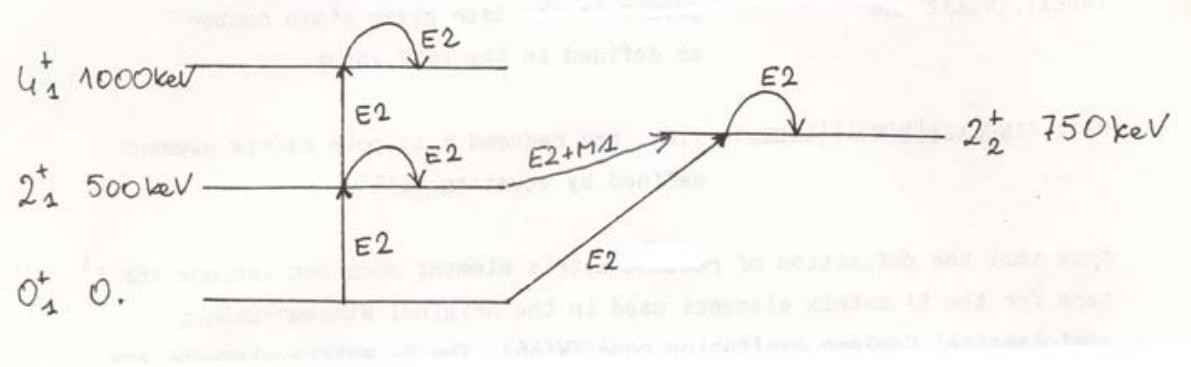
\includegraphics[max width=\textwidth, center]{2025_02_07_204a351db2d7f48b61ebg-156}

Figure 7.3: Model system having 4 states with $E 2$ and $M 1$ coupling. The $2_{1}^{+}-2_{2}^{+}$coupling is assumed to be of mixed $M 1$ and $E 2$ character.

\section*{EXAMPLE:}
An example of the use of the suboptions LEVE and ME for an OP, COUL calculation is given below. Consider the definition for the following nuclear level scheme shown in the figure.

\section*{OP,TITL}
Example of definition of nucleus\\
OP,COUL

\section*{LEVE}
$1,1,0,0 \quad$ - Ground state is given index " 1 ".\\
$2,1,2,0.500$\\
3, 1, 4, 1.000\\
$4,1,2,0.750$\\
0, $0,0,0 \quad$ - Ends LEVE input.\\
ME\\
$2,0,0 \quad$ E2 - matrix elements. All E2 matrix elements\\
$1,2,1.0 \quad$ equal to 1.0 e.barns.\\
1, 4, 1.0\\
2, 2, 1.0 INDEX1 and INDEX2 - in increasing order.\\
$2,3,1.0$\\
2, 4, 1.0\\
$3,3,1.0$\\
4, 4, 1.0\\
7, 0, 0 - Terminates input for E2. Starts input for\\
$2,4,1 \quad$ M1 - matrix element in units of $\mu_{N}$.\\
$0,0,0 \quad$ End ME input.

\subsection*{7.17 ME (OP,GOSI)}
\section*{Mandatory suboption of OP,GOSI}
This suboption of OP,GOSI is used both to input and to catalog the starting set of matrix elements as well as to set constraints on the variation of these matrix elements for the least-squares search procedure. The suboption LEVE must immediately precede ME since the catalog of the matrix elements is performed using the level scheme and state indices assigned using the LEVE command. Up to 999 matrix elements are allowed, however, this upper limit may be smaller depending on the total memory usage. Gosia will output an error if this is the case.

Although similar in many respects, the input to the OP,GOSI version of ME is more extensive than that required by the OP,COUL version of ME (Section 7.16). The OP,GOSI version of ME differs from the OP,COUL version in the following respects:\\
(a) Restrictions are placed on the range over which each matrix element is allowed to vary during the least-squares search procedure. These restrictions are used to prevent the code from finding unphysical solutions. Moreover, these restrictions limit the range of coupling coefficients $\zeta$ over which the $\zeta$ dependence of the $q$-parameters is fitted.\\
(b) Specifications are given defining which matrix elements are to be treated as free variables, and which are to be kept fixed or varied conserving a preset coupling with other matrix elements. This allows a reduction in the number of unknowns by using other knowledge such as lifetime, branching ratio or multiple mixing-ratio data to restrict the number of free parameters used in the least-squares search. Note that lifetimes, branching ratios, multiple mixing ratios and $E 2$ matrix elements also can be included explicitly in the data set used for the least-squares search (See OP,YIEL, Section 7.32). Restrictions on matrix elements can be overridden by the OP,RE,A, OP,RE,C and OP,RE,F options, or conversely, additional restrictions can be imposed using the FIX or LCK command of the suboption CONT without changing the ME input. Input for the OP,GOSI version of ME requires a five-entry record.

A summary of the input format is as follows:

\section*{ME}
$\boldsymbol{\lambda}_{1} \mathbf{0}, \mathbf{0}, \mathbf{0}, \mathbf{0} \quad$ Specify multipolarity.\\
INDEX1, $\pm$ INDEX2, ME $, \mathbf{R}_{1}, \mathbf{R}_{2} \quad$ List of matrix elements for multipolarity $\lambda_{1}$ plus lower $\left(R_{1}\right)$ and upper $\left(R_{2}\right)$ limits.\\
$\boldsymbol{\lambda}_{2}, \mathbf{0}, \mathbf{0}, \mathbf{0}, \mathbf{0} \quad$ Specify multipolarity.\\
INDEX1, $\pm$ INDEX2, ME $, \mathbf{R}_{1}, \mathbf{R}_{2} \quad$ List matrix elements for multipolarity $\lambda_{2}$.\\
$\mathbf{0}, \mathbf{0}, \mathbf{0}, \mathbf{0}, \mathbf{0}$ - Terminates input.\\
Matrix elements for each multipolarity are input as a set preceded by a single record defining the multipolarity, i.e., $\lambda, 0,0,0,0$ where $\lambda=1$ through 6 from $E 1$ through $E 6$ respectively, while $\lambda=7$ for $M 1$ and $\lambda=8$ for $M 2$.

Matrix elements are input as:\\
INDEX1, $\pm$ INDEX2, ME $, \mathbf{R}_{1}, \mathbf{R}_{2} \quad$ INDEX $\#$ is the user-given state number as defined in the LEVE input.\\
$\mathbf{M E}=<\mathbf{I N D E X 2}\|\mathbf{E}(\mathbf{M}) \boldsymbol{\lambda}\| \mathbf{I N D E X 1}>\quad$ The reduced matrix element defined by equation 3.17. It is given in units of e.barns ${ }^{\lambda / 2}$ for $E \lambda$ matrix elements and $\mu_{N} \cdot$ barns ${ }^{(\lambda-1) / 2}$ for $M \lambda$ matrix elements. The sign assigned INDEX2 plays no role in the definition of the matrix element. A negative sign signifies coupled matrix elements as discussed below.\\
$\mathbf{R}_{1}$ and $\mathbf{R}_{2}$ are the lower and upper limits, respectively, between which the given matrix element ME is allowed to vary. Obviously $R_{2}>R_{1}$. Equality of $R_{1}$ and $R_{2}$ implies that this given matrix element is kept fixed at the value ME. Note that in this case, i.e., $R_{1}=R_{2}, R 1$ need not be equal to the ME. For example record $1,2,0.5,2,2$ is equivalent to $1,2,0.5,0.5,0.5$

Fixing matrix elements as in the first example is recommended because of two features of the code. First, when an OP,RE command is used the limits of fixed matrix elements are set as $R_{2}=\left|R_{2}\right|$ and $R_{1}=-\left|R_{1}\right|$. If fixing is done as in the second example the matrix element will be allowed to vary only in one direction, i.e., between $\pm 0.5$. Secondly, when fitting the $q$-parameters, the $\zeta$-ranges are set according to the actual limits $R_{1}, R_{2}$. If fixed matrix elements are released at a later stage during the analysis, then there is less risk of incorrect extrapolation if the approach used in the first example is employed rather than later extending the limits without recalculating the $q$-parameter maps. Note that neither $R_{1}$ nor $R_{2}$ should be exactly zero, use a small number instead.

A negative sign assigned to INDEX2 specifies that the matrix element defined by the pair of indices INDEX1, INDEX2 is not a free variable but is a coupled one. In this case $R_{1}$ and $R_{2}$ are no longer upper and lower limits but the pair of indices of the matrix element to which this matrix element is coupled. The code automatically assigns upper and lower limits to the coupled matrix elements using the upper and lower limits given to the one to which it is coupled while preserving the ratio of the initial values of the coupled matrix elements. These upper and lower limits calculated by the code are used if this coupling is subsequently released. The ratio of coupled matrix elements set by the initial values is preserved in the least-squares search if the coupling is not released.

As an example consider the pair of matrix elements:

$$
1,2,2.0,-4,4
$$

$2,-3,1 ., 1,2$\\
The second statement signifies that the matrix element connecting state 2 to 3 is coupled to the matrix element connecting states 1 and 2 in the ratio:

$$
\frac{M(2 \rightarrow 3)}{M(1 \rightarrow 2)}=+0.5
$$

This ratio will be preserved in the least squares search if this coupling is not released. Limits $\left(R_{1}, R_{2}\right)$ of $-2,+2$ will be assigned by the code to the matrix element connecting states 2 and 3 if the coupling of these matrix elements is subsequently released.

The convention of coupling matrix elements already described is valid only within a single multipolarity. The coupling of matrix elements belonging to different multipolarities is performed by using $100 \lambda+R_{2}$ as input for the index $R_{2}$ of the "dependent" matrix element where $\lambda$ is the multipolarity of the master matrix element. The convention that $\lambda=7$ for $M 1$ and $\lambda=8$ for $M 2$ is still valid.

An important restriction is that there can be only one "master" matrix element with a number of dependents coupled to it if a group of matrix elements are specified to be mutually related. For example, a valid sequence is\\
$1,2,2 .,-4,4 \quad$ E2 set of matrix elements\\
$2,-3,2 ., 1,2$\\
$2,-3,0.5,1,202 \quad$ M1 set of matrix elements\\
This describes the coupling of both the $M 1$ and $E 2$ matrix elements of the $2 \rightarrow 3$ transition to the $E 2$ matrix element connecting states 1 and 2 . The $E 2$ matrix element connecting states 1 and 2 will be treated\\
as a variable; any changes of this matrix element will cause proportional changes in both the $M 1$ and $E 2$ matrix elements connecting states 2 and 3 .

An invalid sequence is

\section*{$1,2,2 .,-4,4 \quad$ E2 matrix elements}
$2,-3,1 ., 1,2$\\
$2,-3, .5,2,203 \quad$ M1 matrix elements

This is invalid because it couples the $M 1$ matrix element to the $E 2$ matrix element $2-3$ which already is a "dependent". Coupling of a set of matrix elements to a fixed one is allowed, it will simply fix the whole set. Nevertheless, it is not allowed to fix the master matrix element using $R_{1}=R_{2}$ of a sign opposite to the matrix element.

For example use of the statement:\\
$1,2,2.0,-4,-4 \quad$ will cause a flip of the signs of all matrix elements coupled to the above matrix element. The correct statement is:\\
$1,2,2.0,4,4 \quad$ Note that it is useful to reiterate that it is not necessary to change the $M E$ input in order to alter constraints etc. in the fitting of matrix elements. The commands OP,RE,A; OP,RE,C; and OP,RE,F can override some constraints introduced by the ME setup, while the FIX and LCK commands of suboption CONT allow addition of new constraints.

\section*{RESTRICTIONS}
Failure to comply with the following restrictions may cause erroneous results or an error message will be printed and the job aborted:\\
(a) Multipolarities must appear in order from lowest to highest starting with $E \lambda$ then $M \lambda$.\\
(b) Matrix elements must belong to the upper triangle, i.e.INDEX1<INDEX2.\\
(c) INDEX values must be in increasing order, i.e. odometer ordering.\\
(d) The limits $R_{2}>R 1$ must be obeyed.\\
(e) Neither $R 1$ nor $R 2$ should be exactly zero.\\
(f) Do not set $R 1=R 2$ with a sign opposite to the matrix element if couplings are made to other matrix elements.

\section*{MATRIX ELEMENT PHASES:}
Note that the phase of a wavefunction is arbitrary. However, to facilitate comparison with models it is best to fix the relative phases of states. Choosing one matrix element between two states to be positive couples the relative phases of the wavefunctions of these two states to be the same. Then the phases of any other matrix elements coupling these two states, relative to the phase of the positive one, are observables. Consequently for typical collective bands it is convenient to choose the primary $\Delta I=2, E 2$ transitions in the band to have a positive phase locking the state wavefunctions of the band to have the same phase. In addition the phase of one strong matrix element connecting two separate collective bands locks the relative phase between the states in these collective bands.

When entering matrix elements in the upper triangle be careful to enter the correct phase remembering that time reversal invariance relates the time-reversed matrix elements by

$$
<J_{1}\left\|T^{\lambda}\right\| J_{2}>=(-)^{J_{1}-J_{2}-\lambda}<J_{2}\left\|T^{\lambda}\right\| J_{1}>
$$

Thus the phase of the matrix elements in the lower triangle is related to the upper triangle phase by the $(-)^{J_{1}-J_{2}-\lambda}$ phase term. Similar care must be taken comparing the observed relative phases with model predictions.

\section*{EXAMPLE:}
To illustrate a typical input consider the example discussed in the previous section, but here used under the OP,GOSI command. Let us assume that the number of experimental data is insufficient to perform a completely model-independent analysis. Then some model is used to couple all the diagonal quadrupole matrix elements to the $0_{1}^{+}-2_{1}^{+}$transition matrix element. In addition, the E2/M1 mixing ratio for the $2_{2}^{+}-2_{2}^{+}$ transition is fixed. The sample input then will be as as follows:

\begin{center}
\begin{tabular}{lc}
OP,TITL &  \\
NUCLEUS DEFINITION FOR OP,GOSI &  \\
OP,GOSI &  \\
LEVE &  \\
$1,1,0,0$ & ground state is given index 1 \\
$2,1,2,0,500$ &  \\
$3,1,4,1,00$ &  \\
$4,1,2,0.750$ &  \\
$0,0,0,0$ &  \\
ME &  \\
$2,0,0,0,0$ & E2 header \\
$1,2,1 .,-2,2$ & free variable \\
$1,4,1,-2,2$ & free variable \\
$2,-2,1,1,2$ & coupled to $E 2 ; 1 \rightarrow 2$ (indices, not spin values) \\
$2,3,1,-3,3$ & free variable \\
$2,4,1,01,5$ & free variable \\
$3,-3,1,1,2$ & coupled to $E 2,1 \rightarrow 2$ \\
$4,-4,1,1,2$ & coupled to $E 2 ; 1 \rightarrow 2$ \\
$7,0,0,0,0$ & ends E2 input, starts M1 input \\
$2,-4,1,2,204$ & coupled to $E 2 ; 2 \rightarrow 4$ \\
$0,0,0,0,0$ & ends ME input \\
\end{tabular}
\end{center}

In this example there are only four variables, i.e. the $1 \rightarrow 2,2 \rightarrow 3,1 \rightarrow 4$ and $2 \rightarrow 4 E 2$ matrix elements. All the diagonal matrix elements are kept equal to the $E 2$ matrix element connecting $1 \rightarrow 2$. The $2 \rightarrow 4 M 1$ matrix element which is equal to and coupled to the $2 \rightarrow 4 E 2$ matrix element.

\subsection*{7.18 OP,MINI (MINIMIZE)}
This command causes execution of the least-squares fitting of matrix elements to the experimental data. Refer to Section 6.7 for an explanation of the procedures used for the least-square search. The starting set of matrix elements used by OP,MINI depends on the other option commands specified. If OP,RAND is specified then OP,MINI uses the set of random numbers generated by OP,RAND as the set of starting matrix elements. If OP,REST is specified, then the starting set of matrix elements is read from file2. If neither OP,RAND nor OP,REST are specified then the matrix elements input using the suboption ME are used as a starting set. Completion of an OP,MINI command causes the set of matrix elements resulting from minimization to be written onto file2. This current set can be used as a new starting point for continued minimization.

The OP,MINI command provides various switches to allow those matrix elements satisfying certain criteria to be locked during the current minimization procedure. This reduction of the number of free variables can greatly speed up the minimization procedure. The FIX command in the suboption CONT provides another mechanism for fixing matrix elements (see Section 7.3). Section 14.4 shows the correct location of OP,MINI in the input stream.

The input to OP,MINI comprises the title plus one record, i.e.

\section*{OP,MINI}
\section*{IMODE,NPTL,CHILIM,CONV,TEST,LOCKF,NLOCK,IFBL,LOCKS,DLOCK}
where:\\
IMODE Mode selector. IMODE should be defined as a four-digit number $I J K L$ where:\\
$\mathbf{I}=1$ or 2\\
$I=1$ specifies that the fast approximation will be used to calculate both $S$ (Eq. 6.73) and its partial derivatives.\\
$I=2$ implies that $S$ will be calculated using the full Coulomb excitation formalism while its derivatives still will be estimated using the fast approximation.

Use of $I=1$ is recommended for almost all applications. The time required to complete the minimization step using $I=2$ is about an order of magnitude greater than when using $I=1$. The use of $I=2$ should be reserved for small cases or for cases requiring extreme accuracy in locating the minimum. The TEST switch, described below, provides a more efficient way of retaining high accuracy than using $I=2$.\\
$\mathbf{J}=0$ or 1\\
$J=0$ selects the simple steepest descent minimization (see Section 6.7.4), while $J=1$ selects the gradient and gradient derivative method (see Section 6.7.5).\\
$\mathbf{K}=0$ or 1\\
$K=0$ implies that the absolute changes in matrix elements will be used to improve the minimum while $K=1$ requests the use of the relative changes. To first order $K=1$ corresponds to using the logarithms of matrix elements as independent variables instead of the matrix elements themselves, as when $K=0$.\\
$\mathbf{L}=0$ or 1\\
$L=0$ specifies that the experimental yields, branching ratios etc. will be used as dependent variables to construct the $S$ function while $L=1$ requests that a logarithmic scale will be used for dependent variables which effectively smooths out the sharp valleys.

There are no restrictions concerning the selection of the above switches and any combination can be used. Proper selection of IMODE can speed up the minimization procedure appreciably and is casedependent

NPTL The maximum number of steps of minimization allowed.\\
CHILIM The $S$ criterion to stop minimization. That is, the minimization terminates if $S<C H I L I M$.\\
CONV The convergence criterion to stop minimization when $\left|\bar{M}_{i+1}-\bar{M}_{i}\right|<C O N V$ where $\bar{M}_{i}$ denotes the vector of matrix elements at the $i$-th step of minimization. This convergence criterion also is used by the iterative search for the minimum along the gradient direction. This iterative procedure is stopped when the absolute difference between two subsequent iterations is less than CONV. Minimization may be resumed after the CONV criterion is fulfilled if $L O C K F=1$ (see below). Note: any of the above three criteria, namely NPTL, CHILIM and CONV, stops minimization if fulfilled. The LOCKF switch resumes minimization only when the calculation was terminated because convergence was achieved. A reasonable value for CONV is $10^{-4}$.

TEST Specifies recalculation of the internal correction factors every time $S$ drops by a factor of TEST. In the limit $T E S T \leq 1$ the internal correction coefficients will be calculated at each step of minimization which corrects for the discrepancy between the value of $S$ calculated using the fast approximation and $S$ coming from the full formalism. Note that this is faster than using $I=2$ since only one full calculation is required per step for $T E S T \leq 1$ whereas each sampling of the minimized function during the onedimensional search along the gradient direction will require a full Coulex calculation using the $I=2$ option.

LOCKF Can equal 0 or 1. $L O C K F=0$ implies that minimization will be terminated if the convergence limit CONV is satisfied. $L O C K F=1$ causes the program to fix the $N L O C K$ matrix elements having the most significant $S$ derivatives. This switch provides a different subspace of matrix elements, which can be useful when trapped in a local minimum or when the matrix elements having weak influence on $S$ should be allowed to vary. As described in Section 6.7, GOSIA will lock the matrix element having the most significant $S$ derivative if the search directions in two consecutive steps are close to being parallel, even if $L O C K F=0$.

NLOCK The number of matrix elements having the largest derivatives of $S$ to be locked if $L O C K F=1$ and the convergence limit CONV is satisfied. See LOCKF.

IFBL May equal 0 or 1. If $I F B F L=0$ then the derivatives are calculated using only the forward difference method whereas $I F B F L=1$ causes the forward-backward difference method to be used for calculation of the derivatives. The $I F B P L=1$ option is justified only in the vicinity of the minimum when the forward difference method may produce spurious results since the $I F B F L=1$ option is a factor of two slower than the $I F B F L=0$ option.

LOCKS May equal 0 or 1 . If $L O C K S=1$ then the code fixes, at the first stage of minimization, all matrix elements $M_{i}$ for which the absolute value of the partial derivative of $S$ with respect to $M_{i}$ is less than DLOCKS (the gradient is always normalized to unity), i.e

$$
\left|\frac{\delta S}{\delta M_{i}}\right|<D L O C K S
$$

This allows an automatic reduction of the number of variables for which derivatives need to be calculated to only those having a significant influence. $L O C K S=0$ switches off this option.

DLOCKS Specifies the limit of the derivative below which a matrix element will be fixed if $L O C K S=1$.

Note that the yields printed by OP,MINI are defined to be

$$
Y^{M i n i}\left(I \rightarrow I_{f}\right)=\frac{Y^{\text {Point }}\left(I \rightarrow I_{f}\right)}{\sigma_{R}\left(\theta_{p}\right) \cdot \sin \left(\theta_{p}\right)}
$$

and do not include $\sigma_{R}\left(\theta_{p}\right) \cdot \sin \left(\theta_{p}\right)$. Note that $Y^{\text {Point }}\left(I \rightarrow I_{f}\right)$ is given by equation 6.38. See also section 7.19, OP.POIN. The experimental values are compared to the calculated $Y^{\operatorname{Mini}}\left(I \rightarrow I_{f}\right)$ which do include the $\sigma_{R}\left(\theta_{p}\right) \cdot \sin \left(\theta_{p}\right)$ term. Thus these missing terms in $Y^{M i n i}\left(I \rightarrow I_{f}\right)$ are absorbed into the normalization constants for each experiment.

\subsection*{7.19 OP,POIN (POINT CALCULATION)}
This option causes execution of a calculation of the $\gamma$-ray yields for one scattering angle and one bombarding energy as specified for each experiment in EXPT. OP,POIN can be used to simulate 'corrected' experimental $\gamma$ yields. In this mode OP,POIN also generates a 'corrected experimental yields file' on file4, which can be used subsequently for simulating the real experiments (e.g. to analyze the influence of the matrix elements on the supposedly observed yields). Note: when executing OP,POIN one should set the experimental yields file selector (NTAP in OP,YIEL input) to 0 - see 5.29. Section 7.4.3 shows the correct location of OP,POIN in the input stream.

The input to OP,POIN is as follows:

\section*{OP, POIN}
IFL, YLIM $\quad I F L=0$ specifies the normal calculation, $I F L=1$ the 'simulation' calculation. $Y L I M$ is redundant if $I F L=0$, whereas if $I F L=1$ it specifies that all transitions whose yield divided by the yield of the normalizing transition (defined in OP, YIEL) exceeds YLIM will be treated as 'experimental observables' and will be included in the file 4 file. OP,POIN will also produce a file containing the $\gamma$ detector efficiency information if OP,RAW was executed and PRT, flag 20 was set to 1 (file23). Note that the decay energies in file23 output are Doppler-shifted.

Note that OP.POIN evaluates the point $\gamma$-ray yield in the laboratory frame for transition $I \rightarrow I_{f}$ that is defined by equation 4.16. That is:


\begin{equation*}
Y^{\text {Point }}\left(I \rightarrow I_{f}\right)=\sin \left(\theta_{p}\right) \int_{\phi_{p}} \frac{d^{2} \sigma\left(I \rightarrow I_{f}\right)}{d \Omega_{\gamma} d \Omega_{p}} d \phi_{p} \tag{6.38}
\end{equation*}


where the integrand is given by


\begin{equation*}
\frac{d^{2} \sigma\left(I \rightarrow I_{f}\right)}{d \Omega_{p} d \Omega_{\gamma}}=\sigma_{R}\left(\theta_{p}\right) \sum_{\substack{k \\ \chi \geq 0}} R_{k \chi}\left(I, I_{f} ; \theta_{p}\right) P_{k \chi}\left(\theta_{\gamma}\right)\left(2 \cos \chi\left(\phi_{p}-\phi_{\gamma}\right)-\delta_{\chi 0}\right) \tag{6.35}
\end{equation*}


Note that $Y^{\text {Point }}\left(I \rightarrow I_{f}\right)$ includes the Rutherford cross section, the $\sin \left(\theta_{p}\right)$ term, integration over the projectile $\phi_{p}$ angle, the deorientation effect and $\gamma$-detector $Q_{K}$ attenuation coefficients.

The total number of coincident $\gamma$-rays detected then is given by

$$
\text { Counts }=10^{-27} \cdot\left[\frac{Q}{\hat{q} e}\right] \cdot\left[\frac{N_{A}}{A}\right] \cdot[\rho d x] \cdot Y^{\text {Point }}\left(I \rightarrow I_{f}\right) \cdot \Delta \theta_{p} \cdot \varepsilon_{p} \cdot \varepsilon_{\gamma} \cdot \Delta \Omega_{\gamma}
$$

where:\\
$Q \quad$ is the integrated beam charge $[C]$\\
$\hat{q} \quad$ the average charges state of the beam\\
$e \quad$ the proton charge $\left[1.602 \times 10^{-19} \mathrm{C}\right]$\\
$N_{A} \quad$ Avogadro number $\left[6.022 \times 10^{23}\right.$ atoms $\left./ \mathrm{mol}\right]$\\
$A \quad$ Target mass number $[\mathrm{g} / \mathrm{mol}]$\\
$\rho d x \quad$ areal target thickness in $\left[\mathrm{g} / \mathrm{cm}^{2}\right]$\\
$Y^{\text {Point }}\left(I \rightarrow I_{f}\right) \quad$ OP.POIN output in $\left[\frac{m b}{s r \cdot r a d}\right]$\\
$\Delta \theta_{p} \quad$ Projectile scattering angle range [rad]\\
$\varepsilon_{p} \quad$ particle detection efficiency per unit solid angle\\
$\varepsilon_{\gamma} \quad \gamma$-ray detector efficiency excluding the geometrical solid angle\\
$\Delta \Omega_{\gamma} \quad$ geometrical solid angle of the $\gamma$-ray detector. Note that usually one only knows the product $\varepsilon_{\gamma} \cdot \Delta \Omega_{\gamma}$

\subsection*{7.20 OP,RAND (RANDOM ME)}
This option generates a set of random matrix elements which replaces the set defined previously for the current job. Each matrix element in the random set is created assuming a uniform distribution of random numbers lying between the limits specified for each matrix element in the input to ME. This option is used to eliminate bias in the analysis and to test the uniqueness of the least-squares fit to a given data set by retrying the minimization starting from a number of sets of random matrix elements. If OP,RAND is used it should immediately precede OP,YIEL.

The input requires only one number:\\
SEED: A floating-point seed number for the internal random number generator. SEED should be larger than unity and less than 32000 . Note that FORTRAN random number generators are reproducible, giving the same sequence of random numbers when called. Therefore SEED should be different for repeated runs, otherwise the results will be identical.

\subsection*{7.21 OP,RAW (RAW UNCORRECTED $\gamma$ YIELDS)}
This option allows defining the $\gamma$-intensities for some, or all, experiments as "raw", that is, the raw $\gamma$ ray yields are not corrected for the detection efficiency. In addition, the raw $\gamma$ intensities can be summed over clusters of $\gamma$ detectors. This latter feature is important when analyzing data from multidetector arrays (crystal balls). Raw counts from the $\gamma$ detectors symmetric with respect to the recoil direction, and correctly Doppler-shifted, can be combined to increase statistics and to reduce the number of datasets that need to be processed (such sets of data will be referred to as "clusters"). GOSIA can handle such raw data, which is not detection-efficiency corrected, provided that the efficiency calibration of the individual detectors also is input separately. This information should be given using OP,RAW and should be executed if at least one experiment involves raw data or clusters. OP,RAW should immediately follow OP,YIEL (7.32). If OP,RAW is to be used, the first entry of OP,GDET (7.10) should be negative to produce the additional file, file8, required by OP,RAW.

Although OP,RAW is designed to handle raw $\gamma$-ray yields not corrected for detection efficiency, it also is very useful for clusters of detectors for which the experimental $\gamma$ intensities already have been detectionefficiency corrected. This feature is possible by making the $\gamma$-ray detector efficiency an energy-independent constant for each individual detector in a cluster as outlined in chapter 7.21.2. As described in chapter 4.6 this option is especially useful for correctly accounting for the $p-\gamma$ angular correlations for partitioning an arbitrary detector shape into a cluster of axially-symmetric detectors. Examples are a GRETINA module of four hexagons or a clover detector.

\subsection*{7.21.1 Input of raw uncorrected $\gamma$-ray yields}
Energy-dependent efficiency calibration for each individual $\gamma$ detector is assumed to follow the functional form used by the code GREMLIN (see Chapter 15).

The input to OP,RAW is as follows:

IEXP Number of experiment to be labelled as raw (according to the sequence of suboption EXPT).\\
A1, A2, ....A8 Logical detector 1\\
A1, A2, ...A8 Logical detector 2

A1, A2, ..A8 Parametrization of efficiency curves for all $\gamma$ detectors used in the experiment IEXP. Parameters $A 1$ through $A 8$ correspond to $a_{0}, a_{1}, a_{2}, a_{3}, f, N, b, c$, as defined in GREMLIN. See Chapter 15. Use $f=0$ to switch off the $F$ factor and $c=0$ to switch off the $W$ factor These sets of parameters should be ordered according to the sequence of "logical" $\gamma$ detectors, as defined in OP,YIEL (7.32) input. The Doppler shift of the $\gamma$ energies is taken into account when evaluating the detection efficiency

NC Number of clusters.\\
ID1 Number of $\gamma$ detectors for cluster \#1.\\
I1, I2..I(ID1) Indices of "logical" detectors forming cluster \#1, according to the sequence defined in OP,YIEL\\
$0 \quad I E X P=0$ ends input.\\
The sequence $I D 1 \ldots$ obviously should be repeated $N C$ times to define every cluster, unless $N C=0$ (no clusters). The whole input is to be defined for every raw experiment. The use of OP,RAW imposes an important constraint on how the experimental $\gamma$ yields should be ordered in either file 3 or file4. The\\
sequence of $\gamma$ yields data sets should follow the HIGHEST "logical" detector index within a cluster. Single detectors can be handled as if they were one-detector clusters, without labeling them as clusters.

OP,RAW can be exploited for clustering the physical detectors of multidetector arrays to fewer logical detectors in order to reduce the number of logical detectors handled by Gosia and improve the statistics per logical detector.

\section*{Example:}
Three $\gamma$ detectors were used and the $\gamma$-ray spectra from the detectors labeled 1 and 3 in OP,YIEL assignment were added. In this case there are two clusters, namely composite detector $1+3$ and single detector 2. The input to OP,RAW should then be as follows:

\begin{center}
\begin{tabular}{ll}
OP,RAW &  \\
1 & experiment \#1 labeled as raw \\
A1....A8 & for logical detector 1 \\
A1...A8 & for logical detector 2 \\
A1...A8 & for logical detector 3 \\
1 & one cluster \\
2 & two detectors in this cluster \\
1,3 & \begin{tabular}{l}
logical detectors forming this cluster \\
0 \\
\end{tabular} \\
ends OP,RAW input &  \\
\end{tabular}
\end{center}

In this case the experimental $\gamma$ yields from detector 2 should precede these from the $1+3$ cluster ( highest logical detector index for the data from detector 2 is 2 , while for $1+3$ cluster it is 3 ).

\subsection*{7.21.2 Input of efficiency-corrected $\gamma$-ray yields for clustered detectors}
OP,RAW is especially useful for handling $\gamma$-ray yields for detector clusters that have already been corrected for detection efficiency. An example involving measurement of angular correlations using Gammasphere assumed logical clusters of 7 detectors comprising a central hexagon plus the six nearest neighbours. This was performed using detection-efficiency corrected data and effectively switching off the OP,RAW efficiency correction by entering efficiency parameters $A 1, A 2, \ldots A 8$ that correspond to a constant detection efficiency. According to the GREMLIN chapter, the efficiency calculated by Gosia can be set to be a constant $\varepsilon=x$ if the following parameters are used:

$$
\begin{aligned}
& a_{0}=0.0 \\
& a_{1}=0.0 \\
& a_{2}=0.0 \\
& a_{3}=0.0 \\
& f=\ln (x) \\
& N=0.0 \\
& b=-50.0 \\
& c=0.0
\end{aligned}
$$

If the individual detectors comprising a cluster have approximately the same absolute efficiency curve, then setting $a_{0}, a_{1}, a_{2}, a_{3}, f, N, b, c$ to $0,0,0,0,0,0,-50$ and 0 respectively switches off the OP,RAW detection efficiency correction. This makes it possible to sum and pass the efficiency-corrected $\gamma$-ray yield data for the cluster to Gosia.

If individual detectors " $i$ " in a cluster have efficiency curves which differ only in the overall normalization, but significantly different absolute efficiencies, $J_{00}$ then the parameter $f$ can be set to equal $\ln \left(\varepsilon_{i}\right)$ for each detector to correct for the difference.

\subsection*{7.22 OP,RE,A (RELEASE,A)}
This option voids all coupling of matrix elements and releases fixed ones. As described in ME (Section 7.17) matrix elements are fixed by specifying identical upper and lower limits $R 1=R 2$. When a fixed matrix element is released these upper and lower limits are set equal to $-|R 2|$ and $|R 2|$, respectively. Consequently, it is useful to use $|R 1|=|R 2|>|M E|$ when fixing matrix elements to ensure that the released matrix element can be varied within an appropriate range.

\subsection*{7.23 OP,RE,C (RELEASE,C)}
This option releases fixed matrix elements but retains the couplings of matrix elements. No additional input is required. As described in 7.17 and 7.18 , when fixed matrix elements are released the upper and lower limits are set equal to $|R 2|$ and $-|R 2|$, respectively.

\subsection*{7.24 OP,RE,F (RELEASE,F)}
This option voids the coupling of matrix elements but retains the fixing of matrix elements. No additional input is required. As described in section 7.18, the upper and lower limits assigned to a coupled matrix element on its release are calculated from the corresponding limits assigned to the master matrix element using the ratio of initial values of the coupled matrix elements.

Note that if OP,RE is used it should immediately precede OP,ERRO or OP,MINI to function correctly.

\subsection*{7.25 OP,REST (RESTART)}
This option causes a set of matrix elements to be read from file12 which then replaces the set defined by the input to ME for the current job. This option enables continuation of a minimization or performing most other operations using the latest set of matrix elements instead of the one appearing in the ME setup. Note that each OP,MINI command causes its final set of matrix elements to be written on file12. If OP,REST is used it should immediately follow OP,YIEL.

OP,REST provides the possibility to manually overwrite some of the matrix elements stored on file 2 for the current job. This feature can be a useful time-saver when, for example, better estimates of some matrix elements have been found during a preliminary diagonal errors calculation. The input to OP,REST should be given as:

\section*{OP, REST}
$\mathbf{I}_{1}, \mathbf{V}_{1} \quad$ Index of the matrix element (according to the sequence of ME )\\
$\mathbf{I}_{2}, \mathbf{V}_{2}$ to be overwritten $(I)$ and its new value ( $V$ ).\\
$\mathbf{0}, \mathbf{0}$ Two zeros terminate input.\\
Example:\\
OP, REST\\
$\mathbf{0}, \mathbf{0}$ This sequence leaves the values stored on file2 unchanged.

Note that if a set of matrix elements is couled to a "master", and only a subset of these will be changed in file 12 , the others will retain their values in the ME section.

\subsection*{7.26 OP,SELE (SELECT)}
This option creates the correlation matrix for use in OP,ERRO. To prepare the input information for SELECT it is necessary to execute OP,MINI with CONT switch SEL, and the default value of the print parameter 4, i.e. $4,-2$. This should be done at a final stage of minimization prior to the error calculation. The information for SELECT is written by GOSIA on file18 which should be attached to SELECT also as file18. No other input is necessary. The output from SELECT is written on file10 and should be attached to the OP,ERRO job as file18. IFC = 1 implies that the correlation matrix will not be used. In this case it is not necessary to create and attach file18. It is however strongly recommended that $I F C=1$ be used only for small cases with all matrix elements of similar significance. Otherwise, selecting $I F C=1$ will dramatically increase the execution time with no effect on the result. $I F C$ is redundant if $I D F=0$.

\subsection*{7.27 OP,SIXJ (SIXJ SYMBOL)}
This stand-alone option creates a 6 -j table to be used by the quadrupole sum-rules program SIGMA (see Chapter 9). OP,SIXJ is not related to an investigated nucleus, thus it can be inserted anywhere in the input stream, even as the only option command. The output is written to a file file14. No further input is required.

Note: The execution of OP,SIXJ will cause GOSIA to stop the job after the $6-j$ symbol table has been written. The remainder of the input will be ignored.

\subsection*{7.28 OP,STAR \\
 (START)}
Execution command to calculate Coulomb excitation amplitudes and probabilities, not the $\gamma$-ray yields, at the "point" energy and scattering angles specified in the EXPT input. This comprises a subset and consequently an alternative to OP,POIN. The OP,STAR requires no input.

Note that OP,STAR is (besides the OP,SIXJ and OP,GDET commands) the only executable option which does not require the $\gamma$-ray deexcitation related information provided using OP,YIEL and thus can immediately follow OP,COUL or OP,GOSI commands.

\subsection*{7.29 OP,THEO (COLLECTIVE MODEL ME)}
Coulomb excitation is the preeminent probe of collective modes in nuclear structure. Consequently frequently it is convenient to calculate Coulomb excitation cross sections assuming a set of matrix elements related by a collective model. OP,THEO generates matrix elements according to the geometrical model following the Bohr-Mottelson prescription ( General Structure of Matrix Elements, paragraph 4-3d in Nuclear Structure) (BOH69). See also chapter 2.4.3.

OP,THEO generates only the matrix specified in the ME input and writes them to the REST file. Therefore it should be used after OP, COUL or OP, GOSI, but before OP,REST command is executed. Fixing, coupling and releasing of the matrix elements is controlled by the ME and CONT commands, the only function of OP,THEO being to create numerical values and write them to the restart file. This allows making model-dependent analyses by specifying the coupling scheme, generating a set of matrix elements and, keeping the values coupled, performing the minimization, thus effectively fitting only geometrical intrinsic moments which can greatly reduce the number of fitted variables. To define the OP,THEO input the user must divide the levels specified in the LEVE input into bands of definite values of $K$ quantum number. The first entry under OP,THEO is the number of bands, which, as an input-saver feature, can be given as a negative integer, in which case the remainder of the input to OP,THEO will be ignored and the contents of the restart file not affected. This is helpful if some matrix elements are added or removed using ME option - OP,THEO then can be easily reactivated.

The OP,THEO input is divided into two loops. The first one is the definition of the bands and the levels ascribed to be band members. As usual, LEVE-defined state indices are used to identify the levels. The second loop is the multipolarity loop, which should exhaust all couplings defined in the ME input. Here for each band-to-band coupling ( band indices being either identical for inband matrix elements or different for interband matrix elements ) one should specify relevant intrinsic moments for a given multipolarity. In general there are three intrinsic moments that could be involved. For in-band or equal- $K$ interband transitions only one of them, marked $Q 1$ is relevant. For non-equal $K$ values generally two moments with the projections equal to the sum and difference of $K$ 's are required ( $Q 1$ and $Q 2$ ), unless one of the $K$ 's is zero, when again only $Q 1$ is needed. For the $K$-forbidden transitions a three parameter Mikhailov formula is used. Thus, in general, three $Q$-values are to be input for each band-to-band coupling. Note that $Q 3$ - a decoupling parameter - is irrelevant if none of the $K$-values assumes the value of $1 / 2$ and $Q 2$ is irrelevant for in-band transitions and for $K$-allowed, one $K=0$ interband couplings. Nevertheless, three numbers are required for each band-to-band coupling.

The specification of multipolarities follows the general convention of GOSIA - E1 through E6 are labeled just by 1 through 6 , while $M 1$ is labeled as 7 and $M 2$ as 8 . The definition of bands and multipolarities should exhaust all couplings included in the ME scheme. It is important that calculated matrix elements fit within the user-specified limits.

The structure of the input to OP,THEO is:

NBANDS Number of user-defined bands. If negative OP,THEO is ignored.\\
K,NLEV Band definition - $K$ of a band, number of levels in band \#1\\
N1, N2......, NNLEV Indices of levels forming band \#1

The above two records should be repeated $N B A N D S$ times to define all bands\\
$\boldsymbol{\lambda}_{1} \quad$ Start of multipolarity loop - first multipolarity\\
$\mathbf{N B}_{\mathbf{i}}, \mathbf{N B}_{\mathbf{j}} \quad$ Band indices\\
Q1, Q2, Q3 Intrinsic moments\\
The above sequence should be repeated until all possible\\
in- and interband couplings for the first multipolarity are exhausted

0,0 Ends first multipolarity definition\\
$\boldsymbol{\lambda}_{2} \quad$ Second multipolarity\\
$\mathrm{NB}_{\mathbf{i}}, \mathrm{NB}_{\mathbf{j}}$\\
Q1, Q2, Q3\\
$\mathbf{0}, \mathbf{0} \quad$ Ends second multipolarity definition

0 Ends multipolarity loop and the input to OP,THEO

\section*{Example:}
Assume an even-even nucleus X with two bands - a ground state band and a gamma-vibrational band. The LEVE and ME setup is as follows:

\section*{LEVE}
1,1,0,0\\
$2,1, .2, .2$\\
Levels $1,2,3$ form the ground-state band, while $4,5,6$ form the gamma band\\
$3,1,4, .5$\\
4,1,2,.7\\
5,1,3,1.1\\
6,1,4,1.5\\
0,0,0,0\\
ME\\
2,0,0,0,0\\
1,2,1,-2,2\\
1,4,1,-2,2\\
2,2,1,-2,2\\
2,3,1,-2,2\\
2,5,1,-2,2\\
2,6,1,-2,2\\
3,3,1,-2,2\\
$3,5,1,-2,2$\\
3,6,1,-2,2\\
4,4,1,-2,2\\
4,5,1,-2,2\\
4,6,1,-2,2\\
5,6,1,-2,2\\
6,6,1,-2,2\\
7,0,0,0,0\\
2,4,1,-2,2\\
$2,5,1,-2,2$

3,5,1,-2,2\\
3,6,1,-2,2\\
Matrix elements on the restart file can be generated by OP,THEO using the following sequence:\\
OP,THEO\\
2 Two bands\\
$0,3 \quad \mathrm{~K}$ of the gsb, \# of levels\\
1,2,3 Level list for the gsb\\
2,3 K of the gamma band, \# of levels\\
4,5,6 Level list for the gamma band\\
2 Multipolarity E2\\
1,1 In-band, gsb\\
$1,0,0 \quad$ Q1, two zeros irrelevant\\
1,2 Interband E2\\
$1,1,0 \quad$ Q1,Q2- Mikhailov formula, none of the $K$ 's $=1 / 2$, so Q3 irrelevant\\
2,2 In-band, gamma band\\
$1,0,0 \quad$ In-band Q1, Q2 and Q3 irrelevant\\
0,0 Ends E2 loop\\
$7 \quad$ M1 loop\\
1,2 Interband M1\\
1,1,0 Q1 and Q2 for Mikhailov formula\\
2,2 In-band M1\\
$1,0,0 \quad$ Q1 for in-band transitions\\
0,0 Ends M1 loop\\
$0 \quad$ Ends multipolarity loop and OP, THEO input\\
As a result, the restart file will be created overriding the values of matrix elements as given in ME input. If the first entry, NBANDS, is changed to -2 OP, THEO will become inactive.

Note that Rachel also incorporates the ability to generate matrix elements using collective models including the Alaga rules, Mikhailov, or K-forbidden relations.

\subsection*{7.30 OP,TITL (TITLE)}
This option requires one input record consisting of up to 80 alphanumeric characters. This string is reprinted as a run title. OP,TITL should appear as the first option command, or follow OP,FILE command if used, since execution is immediate. Otherwise, the title will not appear as a header of the output. OP,TITL can be skipped. If more than one title line is wanted this command can be repeated as many times as desired.

\subsection*{7.31 OP,TROU (TROUBLE)}
This troubleshooting option can be used to pinpoint erroneous experimental data and to check if the minimization is trapped in a local minimum. As described in detail in section 6.7.4, this module analyzes the contribution to $\chi^{2}$ of the deexcitation $\gamma$-ray yields to ascertain if there is an inconsistency in the data. The parameter $r_{k}$ defined in equation 6.120 is a measure of the consistency of the data. That is, it identifies if the current minimum of $\chi^{2}$, with respect to a given matrix element, results from cancellation of large and opposite contributions due to inconsistent data or whether all the data are consistent.

The input consists of one record:

NS, RL $\quad N S$ is the number of experimental yields giving the largest positive and negative components of the derivative of $\chi^{2}$ with respect to a given matrix element to be selected and printed out. This information will appear in the output if for this given matrix element $r_{k}$ exceeds $R L$. The $\chi^{2}$ function is defined by Eq. 6.114.

\section*{NOTE:}
\begin{enumerate}
  \item OP,TROU must be used with, and immediately follow, OP,MINI. OP,TROU must be the last option before OP,EXIT
  \item $\mathrm{OP}, \mathrm{TROU}$ must be used in conjunction with the yields sensitivity map, i.e. print control parameter $I P R M(4)$ in CONT (Section 7.3) must assume its default value equal to -2 .
  \item The OP,TROU analysis will appear at the end of the output file (unit 22).
\end{enumerate}

\subsection*{7.32 OP,YIEL (YIELDS)}
This option is mandatory if it is desired to calculate the yields of deexcitation $\gamma$-rays following Coulomb excitation. The first part of this option is used to input the internal conversion coefficients and the description of the $\gamma$-ray detectors. This first section is used in conjunction with either OP,COUL or OP,GOSI. The second part of this option is used in conjunction with OP,GOSI to input additional information required for the least-squares fitting such as normalization constants, $\gamma$-ray branching ratios, lifetimes, $E 2 / M 1$ mixing ratios, and diagonal or transitional $E \lambda / M \lambda$ matrix element data to be included in the fit. The input to OP,YIEL must be complete and consistent with the option of the code selected. Section 14.4 shows the correct position of OP, YIEL in the input stream for various calculations.

OP,YIEL defines the "logical" $\gamma$ detectors, which are referred to everywhere in the input except in OP,GDET. Different logical detectors may be in fact the same "physical" ones. This distinction allows reducing the number of experiments defined in all cases where the setup used is symmetric with respect to the beam axis. As an example, let us consider the experiment in which two particle detectors are placed symmetrically about the beam axis at angles $(\theta, \phi)$ and $(\theta, \phi,+\pi)$, respectively. Gamma rays are detected in coincidence with scattered particles in one Ge detector placed at position $\left(\theta_{g}, \phi_{g}\right)$, so the scan of event-by-event data yields two $\gamma$ spectra. A straightforward approach is to define two experiments, differing only by the placement of the Ge detector with respect to the scattered particles. Instead, one can define only one experiment (keeping in mind that the Coulomb excitation depends on $\theta$, but not on $\phi$ ) and two logical detectors, one at $\left(\theta_{g}, \phi_{g}\right)$, and another at $\left(\theta_{g}, \phi_{g}+\pi\right)$. Both are identified as the same "physical" detector, but different sets of $\gamma$ yields (both spectra resulting from the scan) are assigned to them. Such a manipulation saves almost $50 \%$ of CPU time since evaluation of deexcitation $\gamma$ yields requires negligible computation time compared to the excitation calculation.

GOSIA allows also to define logical detector clusters (see OP,RAW-7.21), i.e. sets of $\gamma$ yields which result from summing the raw spectra, therefore the number of experimental data sets is not always equal to the number of logical detectors. Further description will refer to the "logical" detectors simply as $\gamma$ detectors, which should be distinguished from either "physical" detectors or data sets.

\section*{Brief resumé of the input to OP,YIEL:}
\section*{OP, YIEL}
IFLAG Assumes the values of 0 or 1. $I F L A G=1$ means that the correction to the angular distribution of the $\gamma$-rays due to a finite distance traveled by the decaying nucleus will be included in the calculation (see Section 6.4). IFLAG $=0$ switches off this correction.

N1, N2 Number of energies $(N 1 \leq 50)$ and multipolarities $(N 2)$ to define the internal conversion coefficients. If $N 1$ is negative the internal conversion coefficients are taken from the table of values for each transition created by $O P, B R I C$.\\
$\mathbf{E}_{1}, \mathbf{E}_{2}, \ldots, \mathbf{E}_{N 1}$ Energy meshpoints for the internal conversion coefficients (in MeV ), common for all multipolarities for the nucleus of interest. The code uses spline interpolation between meshpoints if the recommended option $S P L$, in suboption $C O N T$ is used. Note that the large discontinuities in the internal conversion coefficients at the $K$ and $L$ edges can be taken into account correctly by ensuring that there are at least two mesh points between the transition energy of interest and the nearest discontinuity; that is, so that the four point interpolation does not does straddle any discontinuity. This problem is avoided using $O P, B R I C$.

\section*{I1 Multipolarity I1.}
$\mathbf{C C}(\mathbf{I} 1, \mathbf{1}) . . \mathbf{C C}(\mathbf{I} 1, \mathbf{N} 1) \quad$ Internal conversion coefficients for multipolarity $I 1$ at each energy meshpoint ( $N 1$ entries). Note that internal conversion coefficients can be obtained from the NNDC (US National Nuclear Data center) at \href{http://www.nndc.bnl.gov/bricc/}{http://www.nndc.bnl.gov/bricc/}.

I2 This sequence should be repeated for all multipolarities defined, i.e. N2 times.\\
$\mathrm{CC}(\mathrm{I} 2,1) . . \mathrm{CC}(\mathrm{I} 2, \mathrm{~N} 1)$

NANG(I)..NANG(NEXP) Number of individual $\gamma$-ray detectors for each of the $N E X P$ experiments. Each detector position in the laboratory must be included in $N A N G$. This includes each detector which is used as a separate partition as well as each individual detector that is included in a summed cluster. $N A N G(I)$ is limited to $<200 . N A N G(I)$ can be entered as its true value with a negative sign which means that the $\gamma$ detector setup is identical to that of the previous experiment, for example if the experiments differ only by the scattering angle. In this case the next three records need not be entered.

IP $(\mathbf{1})$..IP(NANG(I)) Identifies the $\gamma$ detectors used in a given experiment according to the sequence the "physical" detectors were defined in the input to $O P, G D E T$ (Section 7.10). For example, if $I P(L)=K$, then it is understood that the $L$-th detector used in the current experiment is the $K$-th detector defined in the $O P, G D E T$ input. This assignment of "physical" detectors to the "logical" ones is the only instance the "physical" detectors are referred to. Everywhere else the $\gamma$ detectors are the "logical" detectors.\\
$\theta_{1}, \ldots \theta_{N A N G(I)} \quad \theta$ angles for $\gamma$ detectors used in experiment $I$.\\
$\phi_{1}, \ldots \phi_{N A N G(I)} \quad \phi$ angles for $\gamma$ detectors used in experiment $I$.\\
The above sequence, starting from the definition of $I P$ should be repeated for each of $N E X P$ experiments defined, except of the experiments for which $N A N G$ is negative. The experiments must be ordered according to the sequence they appear in $E X P T$ input.

NS1, NS2 The transition from $N S 1$ to $N S 2$ to be used as the normalization transition where $N S 1$ and $N S 2$ are the state indices.

End of input for $O P, C O U L$. The remainder of the input is required only if OP,GOSI was specified. The following three lines should be input if $N A N G(I)$ is positive.

NDST Number of data sets in experiment 1. Usually equal to $N A N G(1)$, unless detector clusters were defined in $O P, R A W$.\\
$\mathbf{U P L}_{1} \ldots \mathbf{U P L}_{n} \quad$ Upper limits for all $\gamma$ detectors used in experiment 1.\\
$\mathbf{Y N R M}_{1} \ldots \mathbf{Y N R M}_{n} \quad$ Relative normalization factors of $\gamma$ detectors used in experiment 1.\\
The above three lines should be repeated for all experiments according to the sequence of EXPT, except for those assigned the negative value of NANG. Subscript $n=N D S T$ denotes the number of data sets.

NTAP Specifies the file containing experimental yields. NTAP $=0$ is used when this file is not necessary, e.g. when running OP,STAR or OP,POIN under OP,GOSI. Otherwise $N T A P=3$ or 4 corresponding to file 3 or file4, respectively. NTAP must equal 3 if OP, CORR is executed and must equal 4 if OP,ERRO or OP,MINI is executed.

NBRA, WBRA Number and weight of branching ratio data.\\
$\mathbf{I} 1, \mathbf{I 2}, \mathbf{I} 3, \mathbf{I 4}, \mathbf{B}, \mathbf{D B} \ldots N B R A$ records of branching ratios.

\begin{itemize}
  \item $(I 1 \rightarrow I 2) /(I 3 \rightarrow I 4)=B / D B \quad$ where $I_{1} \equiv I_{3}$ and\\
where $I 1, I 2, I 3, I 4$ are state indices, $B$ is the branching ratio with error $D B$. Note $I 1=I 3$ is the initial state that $\gamma$ decays and $I 2, I 4$ are the final states.
\end{itemize}

NL, WL Number and weight of mean lifetime data.\\
INDEX, T, DT $\quad T / D T$ is the mean lifetime of level $I N D E X$.\\
$\ldots \quad N L$ records, lifetimes in picoseconds\\
NDL, WDL Number and weight of $E 2 / M 1$ multipole mixing ratio data.\\
IS, IF , DELTA, ERROR

$$
\delta \frac{E 2}{M 1}(I S \rightarrow I F)=D E L T A \pm E R R O R
$$

... $\quad N D L$ records\\
NAMX, WAMX Number and weight of known EM matrix element data.\\
LAMBDA, INDEX $_{1}$, INDEX $_{2}$, ME, DME Repeat $N A M X$ times.\\
$L A M B D A$ is the multipole, $E \lambda$ with $\lambda=1,2,3,4,5,6$ and $M 1$ with $L A M B D A=7 . I N D E X_{n}$ is the level index. Note the restriction $I N D E X_{1} \leq I N D E X_{2} . M E$ is the $E \lambda$ or $M 1$ matrix element, in the same units as for the $M E$ input, while $D M E$ is the error, assumed to be symmetrical. In the fit procedure the sign of $M E$ is ignored if $I N D E X 1$ is not equal to $I N D E X 2$. Note that this inpuit sequence was changed in 2006 to include $L A M B D A$ that was needed to allow matrix element input for more than the $E 2$ multipole.

\section*{Extended description of OP,YIEL}
IFLAG Determines whether the effect of the finite distance traveled by the decaying nucleus on the $\gamma$-ray angular distribution is to be included $($ IFLAG $=1)$ or not $(I F L A G=0)$. This effect, taken into account as a first-order correction (see Section 6.4), is important only for the long-living states and should not be included in the cases where all the lifetimes are supposed to be in the subnanosecond range to speed up the calculations. Also, the first-order correction may be inhibited if it is necessary to change the sign of some matrix elements, in which case the lifetimes calculated during the minimization may assume unreasonable values if the matrix elements determining the lifetime of a level happen to be close to zero during the search procedure. In such cases GOSIA will automatically reset IFLAG to 0 if $I F L A G$ was input as 1 . It is recommended to use $\operatorname{IFLAG}=1$ only at the final stage of the minimization, when the signs of the matrix elements are already defined. $I F L A G=1$ should not be used in conjunction with OP,RAND.\\
$\mathbf{N} 1, \mathbf{N} 2 \quad N 1$ is the number of energies used as meshpoints for input of the internal conversion coefficients for the nucleus of interest. Energy meshpoints are presumed to be identical for each multipolarity.\\
a) For $N 1$ positive Gosia uses cubic spline interpolation of the input internal conversion coefficients at these meshpoints. At least one point below the lowest transition energy and one point above the highest are required for reliable interpolation of internal conversion coefficients. Use a reasonable range of internal conversion coefficients to ensure a reliable interpolation. Check the interpolated values at least once by requesting the print-out of internal conversion coefficients (refer to print controls described in Section 7.3). Note that the Lagrangian four point interpolation is not able to take into account the discontinuities which may be present at low $\gamma$ energies due to the $K, L$, etc cutoff edges. GOSIA calculates the $K$ and $L$ edge energies and uses different interpolation functions above the $K$ edge, between the $K$ and $L$ edges, and below the $L$ edge to account for the discontinuities in the internal conversion coefficients at these thresholds. Thus it is necessary to include at least three meshpoints below the $L$ edge and between the $L$ and $K$ edges. Since the interpolation uses two points on both sides of the decay energy, make sure that the discontinuity is separated from the closest decay energy by at least two meshpoints. This is important for converted transitions even if the $\gamma$-ray branches are not observed.\\
b) For $N 1$ negative the internal conversion coefficients are taken from the table of values for each input matrix element that has been created by $O P, B R I C$.\\
$N 2$ is the number of multipolarities for which internal conversion coefficients are given. This must be consistent with the number of multipolarities used for the matrix element setup in $M E$.\\
$\mathbf{E}_{1}, \mathbf{E}_{2}, \mathbf{E}_{3}, \ldots \mathbf{E}_{N 1}$ Input of the energies used as meshpoints for the internal conversion coefficients. Units of MeV .

I1 Multipolarity of the internal conversion coefficients. $I 1=1 \ldots 6$ for $E 1 \ldots 6$ respectively. $I 1=7$ for $M 1$ and 8 for $M 2$.

CC1(I1), CC2(I1),..CCN1(I1) Internal conversion coefficients for multipolarity $I 1$ at the energy meshpoints given above. Repeat the multipolarity, $I 1$, and internal conversion coeffient records $C C$ for all $N 2$ multipolarities.

NANG(1) ...NANG(NEXP) $\quad N A N G$ is the number of individual $\gamma$ detectors for each experiment. Each individual $\gamma$-ray detector location in the laboratory frame frame must be included in NANG. This includes each individual detector which is used as a separate data partition as well as each individual detector comprising a summed cluster, i.e. logical detector. $N A N G$ is limited to $<200$. In many cases, a series of logically different experiments is in fact performed during one "physical" run, for example when position-sensitive parallel-plate particle detectors are used, providing the data for a wide range of scattering angles. For this type of experiment the physical setup of the $\gamma$ detectors remains unchanged, therefore repeating the $\gamma$-detector related input would be redundant. To reduce the unnecessary input, one can enter $N A N G(I)$ as the true value of the $\gamma$ detectors used with a negative sign. It will be understood that the $\gamma$ detector setup is the same as for the previous experiment, in the EXPT input sequence. In this case the next three records should not be input.\\
$\mathbf{I P}(\mathbf{1}), \mathbf{I P}(\mathbf{2}) . . \mathbf{I P}(\mathbf{N A N G}(\mathbf{I})) \quad$ The definition of the "physical" $\gamma$ detectors used in an experiment I according to the sequence of OP,GDET.\\
$\boldsymbol{\theta}(\mathbf{1}), \boldsymbol{\theta}(\mathbf{2}), \ldots \boldsymbol{\theta}(\mathbf{N A N G}(\mathbf{I})) \quad$ The angular coordinates $(\theta, \phi)$ in degrees of each $\gamma$ detector in the same coordinate frame as used for the EXPT input for this experiment.\\
$\boldsymbol{\phi}(\mathbf{1}), \boldsymbol{\phi}(\mathbf{2}), \ldots \boldsymbol{\phi}(\mathbf{N A M G}(\mathbf{I})) \quad$ The $z$ axis always is in the direction of the incident beam.\\
N.B. It is recommended that for each experiment the $\gamma$-ray detector giving the best quality data be selected as detector number one. This is because only $\gamma$-ray detector number one is taken into account for certain features of the code, namely, generation of the yield sensitivity maps, i.e. $\left(\frac{\partial \ln (Y \operatorname{IELDS}}{\partial \ln (M E)}\right)$ and the consistency tests performed by the troubleshooting routine OP,TROU.

The sequence of input records starting from the definition of $I P$ must be repeated for all experiments $N E X P$ as defined in EXPT input, except when $N A N G$ is negative for a given experiment.

NS1, NS2 The transition from the state with index $N S 1$ to the state with $N S 2$ is chosen as a normalizing transition. Make sure that the energy of state $N S 1$ is higher than that for state $N S 2$. The transition is common to all experiments. It is used for setting upper limits of unobserved $\gamma$-ray transitions and for printout compiled by OP,POIN.

The input to $O P, Y I E L$ required by $O P, C O U L$ ends at this point. The remainder of the input is related to the least-squares fitting and needs to be entered only for OP,GOSI. The following three lines should be input if $N A N G(I)$ is positive.

NDST Number of data sets for this experiment. This is equal to the number of individual $\gamma$ detectors that are not summed into a cluster, plus the number of clusters defined in OP,RAW for this experiment. $N D S T \leq 32$, while up to 20 clusters per experiment can be defined.\\
$\mathbf{U P L}_{1} \ldots \mathbf{U P L}_{n} \quad$ These are the upper limit $\gamma$-ray yields expressed as a fraction of the normalizing transition, $N S 1 \rightarrow N S 2$. The number of entries in each record corresponds to the number of data sets for each experiment defined, i.e. $n=N D S T$. If the calculated yield of any unobserved $\gamma$-ray transition, divided by the yield of the normalizing transition, exceeds $U P L$, then it is included in the calculation of the least squares summation used for the fit. Otherwise, the unobserved transitions whose calculated yields are below the limit of detection for a particular experiment are not included in the least squares fit procedure. (See Section 6.7).\\
$\mathbf{Y N R M}_{1} \ldots \mathbf{Y N R M}_{n} \quad Y N R M_{i}$ is the relative normalization factor for Ge detector $i$ used in experiment $I E X P$. GOSIA does not require the absolute normalization for a given experiment, instead, the code finds the best normalization constant correlating calculated and experimental $\gamma$ yields. See record $L N$ in suboption $E X P T$ (section 7.8). For each $\gamma$ detector $i$ used in experiment $I E X P$ the calculated and experimental $\gamma$ yields are correlated by:

$$
Y_{i}^{\exp }=Y_{i}^{\text {calc } *} C_{i}(I E X P)
$$

where $C_{i}(I E X P)$ is the normalization constant for experiment $I E X P$ and detector $i$. The code fits the common normalization factor for all $\gamma$ detectors used in a given experiment $I E X P, C(I E X P)$, related to the individual $\gamma$ detectors' normalization factors $C_{i}(I E X P)$ by:

$$
C_{i}(I E X P)=C(I E X P) * Y N R M_{i}(I E X P)
$$

Different experiments may have a known relative normalization, e.g. when different projectile scattering angle slices are defined as experiments. In this case the physical setup, i.e. the location of $\gamma$ detectors etc. is the same for a whole group of experiments and their relative normalization is set only by the Rutherford cross sections and the efficiencies of the particle detectors for specified scattering angle ranges. The known relative normalization may be used by specifying the proper normalization control $L N$ indices in the EXPT input, then the code will use given $Y N R M_{i}(I E X P)$ values to fit the common $C(I E X P)$ value for the whole subgroup of experiments, the definition of $C_{i}(I E X P)$ for individual $\gamma$ detectors remaining the same.

For beam (projectile) detection experiments, $Y N R M_{i}$ should be given by the following formula

$$
Y N R M_{i}=\left(\frac{\partial \sigma_{\text {Rutherford }}}{\partial \Omega}\right)_{\theta_{\mathrm{lab}}^{\text {man }}} \times \sin \left(\theta_{\mathrm{lab}}^{\mathrm{mean}}\right) \times \epsilon_{\mathrm{Ge}} \times \epsilon_{\mathrm{p}}
$$

where $\theta_{\text {lab }}^{\text {mean }}$ is the mean projectile scattering angle in the laboratory frame, and $\epsilon_{\mathrm{Ge}}, \epsilon_{\mathrm{p}}$ are the relative efficiencies of the germanium and particle detectors, respectively. If the $\gamma$-ray yields have been corrected for the relative Ge efficiency, then $\epsilon_{G e} \equiv 1$.\\
For independently normalized experiments ( $L N=$ the experiment number), then


\begin{equation*}
Y N R M_{i}=\epsilon_{\mathrm{Ge}} \tag{7.5}
\end{equation*}


should be entered instead.\\
In the present version of Gosia, if target (recoil) detection is specified for a logical experiment, then this experiment should be normalized independently. That is, it should not be normalized to any other experiment, nor should any other experiment be normalized to it (regardless of whether the other experiment is for target detection).

The RACHEL GUI calculates the correct YNRM values (with the same restriction for target detection) assuming that all $\gamma$-ray yields are efficiency-corrected for the relative efficiency curve of each Ge detector defined. Note that it is possible to request independent normalization for each individual $\gamma$ detector by using the $C O N T$ switch $I N R$,. In this case the $Y N R M$ input is redundant. The normalization constants calculated using user-supplied information are printed by the code along with the recommended relative $Y N R M$ values calculated independently for each $\gamma$ detector.

Consider the example of ${ }^{72}$ Ge discussed in the description of EXPT (see section 7.8). Assume that there are two $\gamma$-detectors for each experiment and that the correction needs to be made to the detection efficiency of the second detector. An input of the form:

\section*{2}
0.05,0.10

1,0.7\\
2\\
0.02,0.03\\
1.,0.6\\
means that unobserved transitions will contribute to the least-squares sum when their calculated yield intensities exceed:

EXPT \# $\quad \gamma$-Detector $\#$

\begin{center}
\begin{tabular}{lll}
1 & 1 & $5 \%$ of normalization transition \\
1 & 2 & $10 \%$ of normalization transition \\
2 & 1 & $2 \%$ of normalization transition \\
2 & 2 & $3 \%$ of normalization transition \\
\end{tabular}
\end{center}

and the normalizations constants are:\\
EXPT \# $\quad \gamma$-Detector $\#$

\begin{center}
\begin{tabular}{lll}
1 & 1 & C1 calculated by the code \\
1 & 2 & $0.7^{*} \mathrm{C} 1$ \\
2 & 1 & C 2 calculated by the code \\
2 & 2 & $0.6^{*} \mathrm{C} 2$ \\
\end{tabular}
\end{center}

NTAP Specifies the number of the file on which the experimental yields reside. NTAP can have values of 3 or 4 corresponding to file 3 or file 4 . The file of original experimental yields is modified to correct for the difference between full Coulomb excitation calculations, integrated over detector solid angles as well as target thickness, and point calculations at fixed scattering angle and incident energy. This modified file of experimental data is used for the least squares minimization and error estimation in conjunction with point calculations. This correction is performed by the OP,CORR command (see Section 6.5.1 and Section 7.4) which reads the unmodified experimental yields from file 3 and writes the corrected experimental yields in file4. Consequently, $N T A P$ must equal 3 when OP,CORR is used. The least-squares minimization and error estimation require the corrected yields. In this case, NTAP should be consistent with the file assignment given in the computer control statements preceding this program. NTAP must equal 4 when OP,ERRO is executed with the $C O N T S M R$, switch because file3 is then reserved for the output needed by the quadrupole sum-rules program SIGMA. NTAP may equal 0 when experimental yields are not required, e.g. when running OP,STAR or OP,POIN under OP,GOSI. $N T A P=0$ implies that the code will not attempt to find and read in the experimental yields file. This would be appropriate for reintegration of the predicted yileds using $O P, I N T I$.

NBRA, WBRA Are the number of experimental branching ratios to be input and weighting factor, respectively. A maximum of 50 branching ratios can be input. If $N B R A=0$ then no further input of branching ratios is required. The weighting factor, $W B R A$, is defined for all the branching ratios used in the least-squares summation. Thus, normally $W B R A=1.0$. It can be helpful, during minimization, to switch off $(W B R A=0)$ or reduce the weight of the branching ratio data to eliminate a problem caused by trapping of the search in the narrow valleys resulting from accurate branching ratio data. For example, branching ratio data can cause the search to be trapped in a solution having the wrong sign for a given matrix element.

If $N B R A$ is not zero then the input is as follows:\\
$\mathbf{I} 1, \mathbf{I 2}, \mathbf{I} 3, \mathbf{I} 4, \mathbf{B}, \mathbf{D B} \quad$ Repeated $N B R A$ times\\
where I is the level index specified in the LEVE input. The branching ratio $B$ with error $D B$ is defined by the ratio of $\gamma$-ray intensities:

$$
\frac{I 1 \rightarrow I 2}{I 3 \rightarrow I 4}=B \pm D B
$$

NL, WL Are the number of experimental mean lifetimes to be input and the weighting factor where $N L \leq 50$. If $N L=0$ then no further lifetime records need to be input. The weighting factor, $W L$, is used for all the lifetime data in the least-squares summation. Normally, $W L=1$. The weighting factor can be set to a smaller number or zero if it is desired to reduce or switch off, respectively, the influence of the lifetime data.

INDEX, T, DT $\quad N L$ records. $I N D E X$ is the index of the level, specified in the input to LEVE. $T$ is the mean lifetime, in picoseconds $\left(10^{-12}\right.$ secs $)$, of the level.\\
$\cdots \cdot \quad$ Note, it is not the half-life $T_{1 / 2}=\ln (2) *. T . \quad D T$ is the error of the mean lifetime in picoseconds.\\
NDL, WDL Are the number of experimental $E 2 / M 1$ mixing ratios to be input and the weighting factor. $N D L \leq 20$. If $N D L=0$ no further mixing ratio records are required. The weighting factor, $W D L$, is used for all the data points in the least-squares summation. Normally, $W D L=1.0$. $W D L$ can be made smaller or zero to reduce or switch off the influence of the mixing ratio data.

IS, IF, DELTA, ERROR $\quad N D L$ records of mixing ratios. $D E L T A$ is the $E 2 / M 1$ mixing ratio for the transition from level $I S$ to level $I F$. It is defined as:

$$
D E L T A=\partial\left(\frac{E 2}{M 1}\right)=0.835 E_{\gamma}(M e V) \frac{<I F\|M(E 2)\| I S>}{<I F\|M(M 1)\| I S>}
$$

Note that the phase convention used is that of Krane [KRA70]. See [KRA70] for a discussion of the various phase conventions. $E R R O R$ is the error in the mixing ratio. Note the error is assumed to be symmetric to assure continuity of the least squares function.

NAMX, WAMX The number of experimental $E \lambda / M \lambda$ matrix elements ( $N A M X$ ) to be input and the weighting factor $(W A M X)$. If $N A M X=0$ no more input is required. The weighting factor, $W A M X$, is common for all the matrix elements used in the least-squares summation. Normally $W A M X=1.0$. $W A M X$ can be made smaller or zero to reduce or switch off the influence of these additional data, $N A M X \leq 100$

LAMBDA, INDEX $_{1}$, INDEX $_{2}$, ME, DME Repeat $N A M X$ times.\\
$L A M B D A$ is the multipole, $E \lambda$ with $\lambda=1,2,3,4,5,6$ and $M 1$ with $L A M B A=7 . I N D E X_{n}$ is the level index. Note the restriction $I N D E X_{1} \leq I N D E X_{2} . M E$ is the $E \lambda$ or $M 1$ matrix element, in the same units as for the $M E$ input, while $D M E$ is the error, assumed to be symmetrical. In the fit procedure the sign of $M E$ is ignored if $I N D E X 1$ is not equal to $I N D E X 2$.

The input of known electromagnetic matrix elements concludes the input to OP,YIEL. The experimental deexcitation $\gamma$-ray yields are input separately as described in Section 7.33.

\subsection*{7.33 Input of experimental $\gamma$-ray yields from Coulomb excitation}
There are two methods to input the experimental $\gamma$-ray yields for use for least-squares fits of the matrix elements to experimental data. The direct method, implemented in the 1980 version of Gosia, involves an inflexible format for specifying the initial and final level indices needed to identify each input yield value. This method is especially inflexible to any change in the level or band structures. The 2011 method implemented in Rachel, and described in chapter 8.4.5, uses names to identify bands which provides flexibility for addition or removal of levels or bands. In addition it allows direct input of Radware ags files of yield data.

\subsection*{7.33.1 Direct input of $\gamma$-ray yield data using the original Gosia format:}
The experimental $\gamma$-ray yields from the Coulomb excitation experiments should be put in a separate file 3 . (See also OP,FILE in section 5.9). GOSIA then creates file4 if OP,CORR is executed.

The structure of the file is as follows:

IEXP, NG, ZP, AP, EP, ND, WT This header record appears before the experimental yields for each experiment and data set.

IEXP This is the experiment number. The experiments must be input in the same order as used for EXPT and OP,YIEL.

NG Number of data sets for experiment $I E X P$. It is equivalent to the OP,YIEL input $N D S T$.\\
ZP Charge number of the projectile.\\
AP Mass number of the projectile.\\
EP Bombarding energy of the projectile ( MeV ).\\
ND Number of experimental $\gamma$-ray yields to be input for the specific $I E X P$ and data set.\\
WT The weighting factor assigned to a given data set (see Eq. 6.73). Normally $W T=1.0$. This weight factor can be made less than one or zero to reduce or switch off respectively the influence of this particular data set.

All the entries of the header, except $W T$ and $N D$, are used only for reprint of experimental data, therefore using the values defined in EXPT and OP,YIEL inputs is not strictly required. Nevertheless, it is recommended to enter $I E X P, Z P, A P, E P$ and $N G$ according to the previous definition to make sure that the sequence of experimental yields is correct.

Each header should be trailed by $N D$ records for that particular experiment and data set. The format is:

\section*{II, IF , Y, $\boldsymbol{\Delta} \mathbf{Y}$}
where:\\
$I I \quad$ Initial level index.\\
$I F \quad$ Final level index.\\
$Y, D Y \quad$ The arbitrarily normalized $\gamma$-ray yield for transition\\
$I I \rightarrow I F$ with absolute experimental error $\pm \Delta Y$.\\
For unresolved doublets, consisting of the $I I 1 \rightarrow I F 1$ transition plus the $I I 2 \rightarrow I F 2$ transition, the input format is: $(100 * I I 1+I I 2),(100 * I F 1+I F 2), Y_{1}+Y_{2}, \Delta\left(Y_{1}+Y_{2}\right)$ where:

$$
\begin{array}{ll}
I I 1, I I 2 & \text { Are the initial level indices for transition } 1 \text { and } 2 . \\
I F 1, I F 2 & \text { Are the final level indices for transition } 1 \text { and } 2 . \\
Y_{1}+Y_{2}, \Delta\left(Y_{1}+Y_{2}\right) & \text { Is the summed yield of the unresolved transitions } \\
& I I 1 \rightarrow I F 12 \text { and } I I 2 \rightarrow I F 2 \text { with error } \pm \Delta\left(Y_{1}+Y_{2}\right) .
\end{array}
$$

There are no restrictions regarding the sequence of the experimental data within the single data set. Data sets within an experiment should be ordered according to the highest logical detector index. If no clusters are defined (see OP,RAW) this is equivalent to ordering the data sets according to the sequence of logical detectors defined in OP,YIEL.

Below is an example of an experimental $\gamma$-ray yield data file for a ${ }^{20} \mathrm{Na}$ beam at 34 MeV . Experiments 1 and 2 have two physical $\gamma$-ray detectors each, while experiment 3 has one. Note that the header is repeated for each detector. The third experiment measured an unresolved doublet of the $7 \rightarrow 6$ and $5 \rightarrow 4$ transitions. The second detector in experiment 2 is weighted 0.5 .

\begin{verbatim}
1,2,11,20,34,2,1.
2,1,634.,6.
3,2,247.,3.
1,2,11,20,34,1,1.
2, 1, 454., 10.
2,2,11,20,34,2,1.
2, 1, 74., 13.
3, 2, 40., 10.
2,2,11,20,34,3,0.5
2, 1, 722., 32.
4, 3, 392., 20.
3, 2, 302., 13.
3,1,11,20,34,1,1.
705, 604, 9.6, 1.1
\end{verbatim}

\subsection*{7.33.2 Rachel format for input $\gamma$-ray yield data:}
The Rachel format for input of experimental $\gamma$-ray yield data is described in chapter 8.4.5.

\section*{Chapter 8}
\section*{RACHEL: A graphical user interface }


\begin{abstract}
RACHEL is a graphical user interface (GUI) for GOSIA written entirely in Python 2.6. This chapter addresses the Rachel version 1.0. The purpose of Rachel is to allow the user to quickly develop inputs to the Gosia code for standard problems and to run Gosia calculations and fits of matrix elements without editing the Gosia input by hand-working entirely within the GUI. The Rachel code understands Radware ascii gated level scheme (AGS) files and is able to read both the level scheme and, optionally $\gamma$-ray yield data from the AGS files or text files. By automatically generating ELAST or SRIM stopping power values and using the BRICC internal conversion calculation option of Gosia, the input file generation is completely automated, except for several input prompts by the terminal for the user which are preceded by explanatory notes. The process of setting up the calculation is further streamlined for large level schemes of collective nuclei by allowing the user to define entire sets of matrix elements using standard models (rotor, Mikhailov rotation-vibration coupling, etc.) in a single command. Matrix element couplings, $B(M \lambda)$ values, $\gamma$-ray yield data (measured and calculated) can be instantly displayed graphically, so that the user does not have to extract these items from a lengthy Gosia output file. This greatly facilitates fitting and analysis. If a non-standard problem needs to be treated, the GUI can be used to generate a basic template input file, which the user can modify by hand and use to run Gosia independently of the GUI. One major advantage of starting to learn Gosia using Rachel is that the GUI has the ability to quickly generate simulated data with optional random scatter of the yields, which can aid users in planning experiments. That is, a simulated set of the desired measurements can be made assuming the proposed experimental parameters, and the predicted uncertainties in the fitted matrix elements can be used in experimental proposals.
\end{abstract}

\subsection*{8.1 Introduction}
The standard input to GOSIA [GOS08] is long and time-consuming to write and debug, especially for collective systems where many hundreds of matrix elements need to be included. The time-saving and instructive prompting features described below not only streamline analysis of data from an experiment that has already been collected, they solve an unfortunately common problem in Coulomb excitation experiments: an experiment is performed, and there may be a wealth of data, but it only becomes clear after spending months of analysis that the data will not yield the quantity that was desired, or with useful precision, or that a semi-classical code such as GOSIA is inappropriate for the experiment. The push-button controls, instructive input prompts, the "Help" button, automated accuracy-testing features, and data simulation capabilities of RACHEL are designed to aid in analysis as well as experiment planning with predicted uncertainties in measurements. Studying the Coulomb excitation analysis techniques to find the best approach, before a proposal is submitted, can provide a tremendous benefit to planning.

A graphical display of matrix elements and functions to add many matrix elements using rotor, rotorvibrator models etc. provide a tremendous speed advantage to the user in setting up calculations for large level schemes, including an automated re-ordering of the matrix according to the needs of GOSIA, when matrix\\
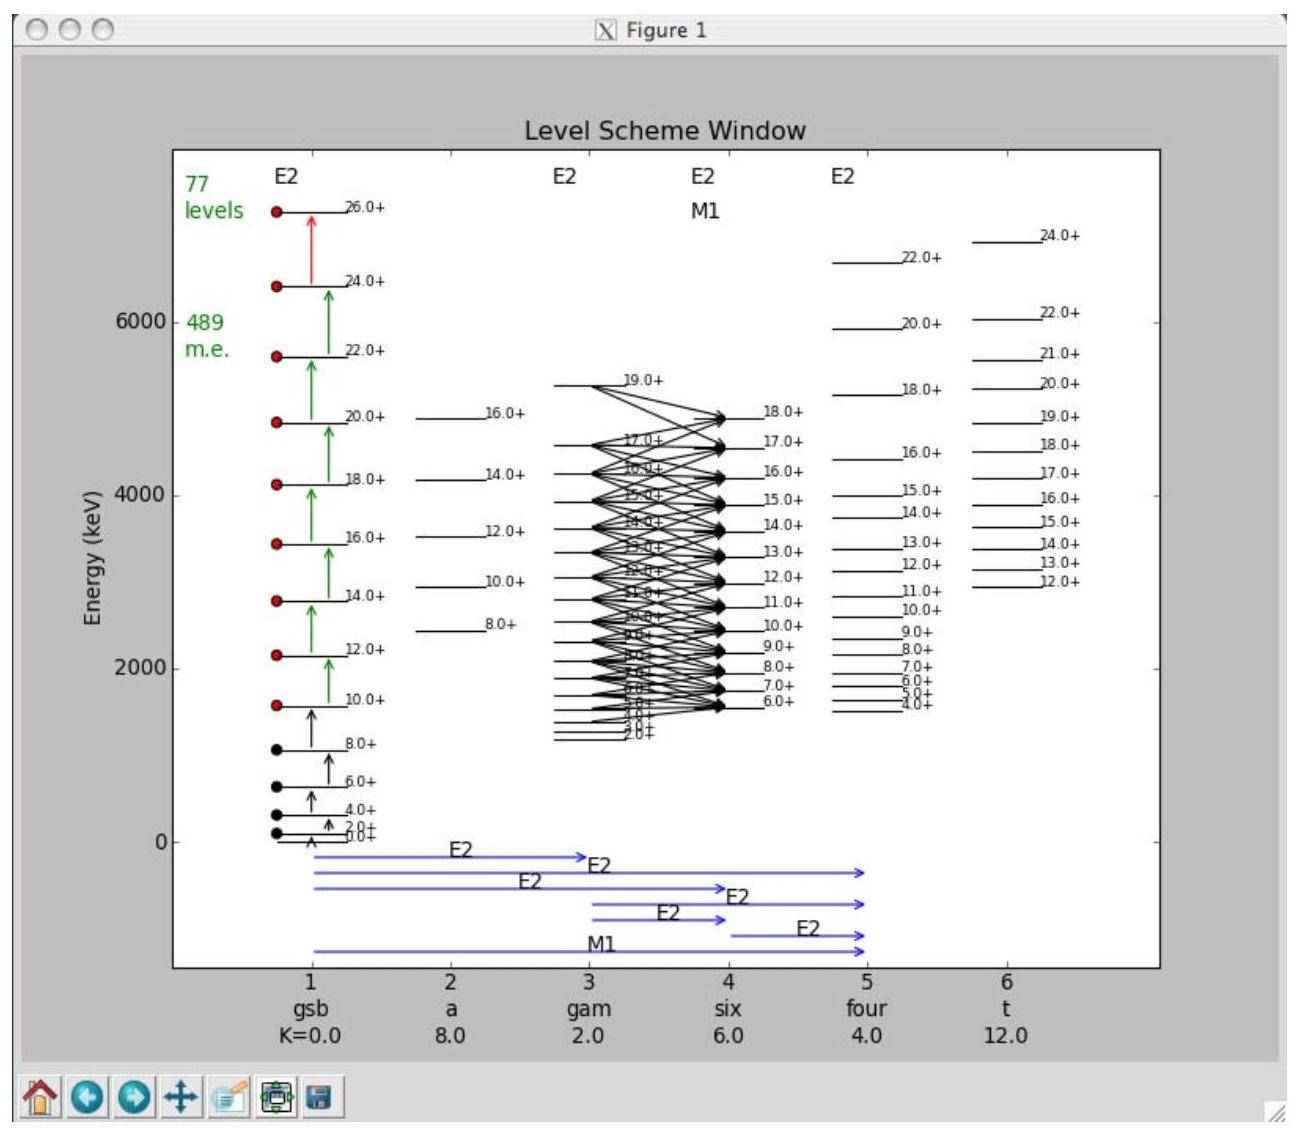
\includegraphics[max width=\textwidth, center]{2025_02_07_204a351db2d7f48b61ebg-188}

Figure 8.1: The RAChEL level scheme display shows the couplings between bands (blue arrows labeled with the multipolarity), in-band couplings ("E2" and "M1" at the tops of bands), fixed matrix elements (not variable in fits) shown as black arrows between levels, selected master (fit parameter) matrix elements shown as green arrows between levels, and matrix elements dependent on the masters displayed as red arrows.\\
elements or levels are added or removed (Fig. 8.1). An upcoming version is expected to have additional tools to visualize data and highlight conflicting data in fits such as illustrated in Fig. 8.2.

In addition to the electromagnetic parameters, GOSIA requires a significant amount of information from the user to describe the laboratory experiment. This includes beam and target species, particle and gammadetector geometries, and beam energy ranges as the beam traverses the target. It can simulate a $4 \pi$ array such as Gammasphere[GS98], or treat individual Ge detectors defined by the user. The only restrictions on the layout of the Ge arrays are in the maximum number of Ge detectors as described in the GOSIA manual. The user-expandable library of Ge detector types and arrays provides a tremendous increase in speed and ease in preparing setup. When gosia inputs are written by hand, stopping power meshpoints as a function of beam energy must be interpolated by the user and given as input data. Iterated energy loss calculations must be performed to find the exit energy for thin targets or range for thick targets. Internal conversion coefficients also must be interpolated and given to GOSIA, with special attention given to the interpolation near electron binding energy edges. All of this information is calculated by RACHEL from a few simple parameters given by the user and passed to GOSIA. A growing library of the properties of major $\gamma$-ray detector arrays (Gammasphere, Miniball, Tigress, etc.) is included in version 1.0 to further speed the setup.

For collective systems, it can be very time-consuming to calculate sets of matrix elements and add them in the proper "odometer" order in the GOSIA input, while removing a rotational band from the calculation is tedious and prone to error, since it requires a complete re-numbering of excited state numbers and matrix element indices. Rotational bands can be added or removed easily using RACHEL, and rotor model or other systematics can be used to quickly create and add or replace sets of matrix elements. Couplings of matrix elements to one parameter for fitting can also be done quickly with the GUI, by describing the set of matrix\\
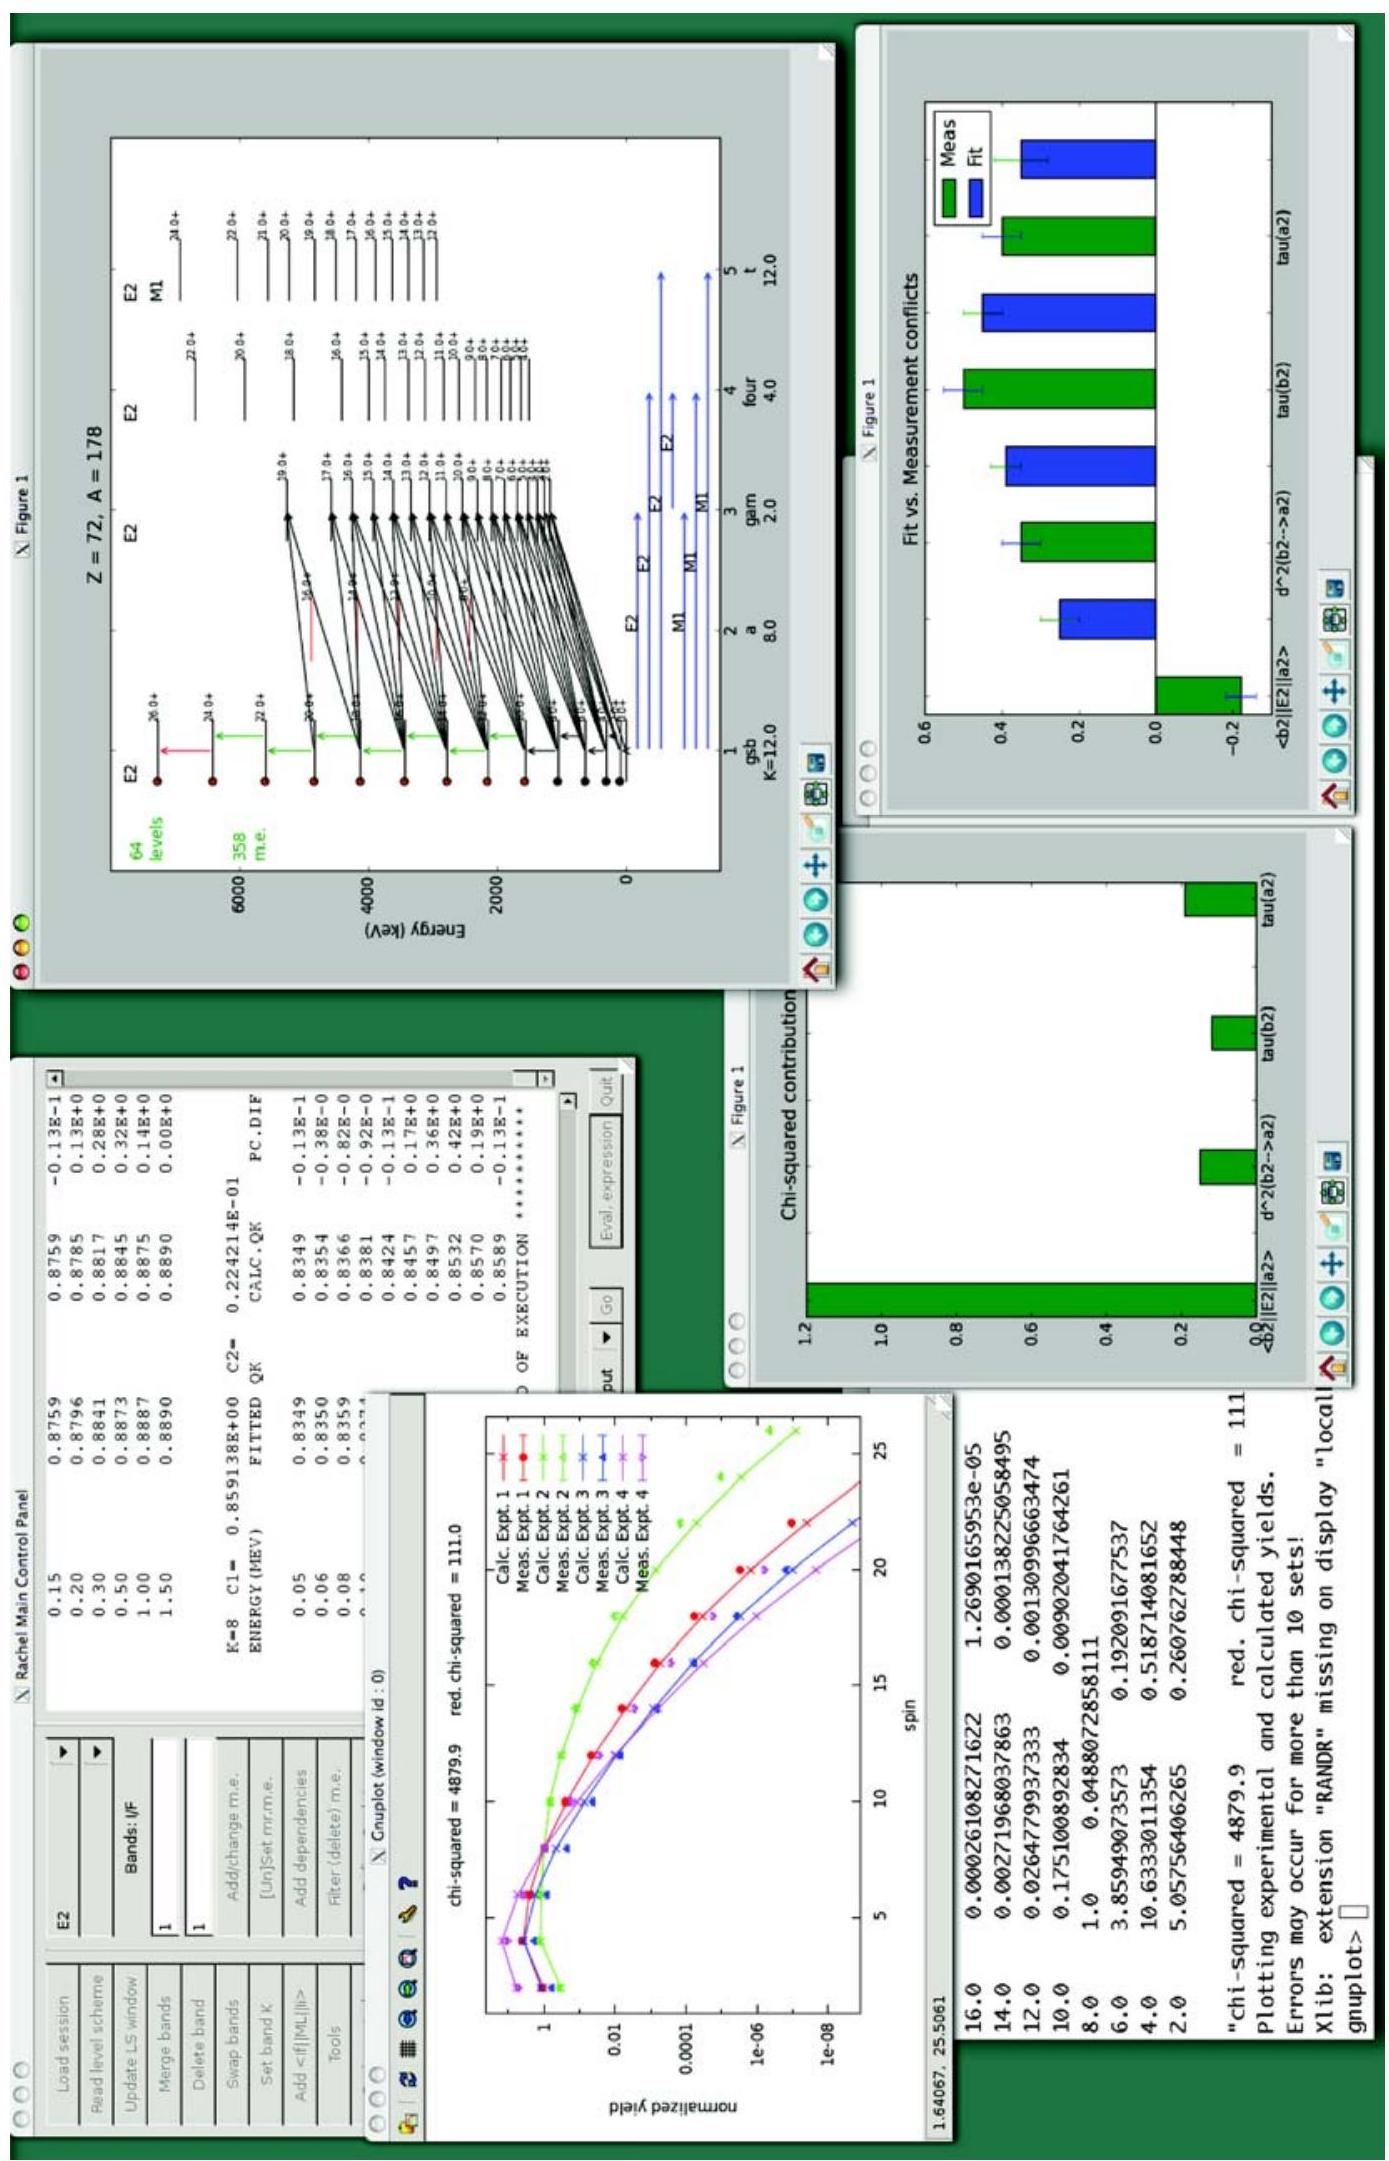
\includegraphics[max width=\textwidth, center]{2025_02_07_204a351db2d7f48b61ebg-189}

Figure 8.2: The plotting features (scatter plot and level scheme) available in version 1.0. Data visualization windows (bar plots) will be implemented in an upcoming version.\\
elements to be coupled and assigning limits for the fit to one "master" matrix element. These parameters can be decoupled and fixed again with simple commands.

Bands that the user has deleted from the GUI's level scheme can be re-introduced at any time by re-reading the level scheme file and deleting the duplicate bands. This means that bands can be deleted from memory or added from the original level scheme file to fit matrix elements to different excited bands. This makes it relatively simple to fit the matrix elements to strongly-populated bands in a first fit, and then iterate the fit as weakly-populated bands are added. As GOSIA's memory permits ( $<100$ levels and $<1000$ matrix elements), decoupled levels can be left in the level scheme. RACHEL will de-select nuclear and $\gamma$-ray yield data as appropriate for decoupled states.

The entire session can be saved at any time, so that the user can revert to previous calculations or fits. Automated crash-recovery and "Undo," "Redo" buttons allow the user to quickly recover from mistakes or system crashes, while running on remote machines.\\
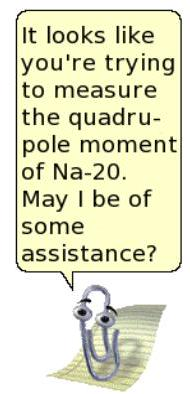
\includegraphics[max width=\textwidth, center]{2025_02_07_204a351db2d7f48b61ebg-190}

Figure 8.3: Popup help windows.\\
RACHEL gives descriptive prompts for information as well as optional pop-up tips to help the novice user with the typical order of operations (Figure 8.3). A "Help" button and tutorial videos on the RaChel website are also available. (These videos in mp4 format can be played on most systems without downloading a new plug-in.) The library of tutorial videos is being updated for version 1.0 as of the release date of this manual.

The GUI handles normal and inverse kinematics for either beam or projectile excitation. Both annular (or on-axis circular) particle detectors with azimuthal scattering symmetry as well as arbitrary polygon detectors are treated by version 1.0. Rectilinear detectors are automatically converted to accurate $\theta(\phi)$ shape sampling data in the GOSIA format as illustrated in figure 8.4. The current version handles most arbitrary detector shapes except for PIN diode arrays and off-axis circular detectors.

The GUI assumes that all $\gamma$-ray yield data are efficiency corrected for the relative efficiency as a function of $E_{\gamma}$, including differing relative efficiencies of each Ge detector and the low-energy effects of absorbers, if any were used. Currently there is no plan to handle non-efficiency-corrected yields.

Many accuracy, data handling and fit parameters are adjustable in Rachel 1 under the button "Gosia controls" including weights of the nuclear data sets.

If it is necessary to use one of the many capabilities of GOSIA that is not currently treated in the GUI, then a basic GOSIA input can be generated, saved to disk and edited as desired. Once a basic calculation is defined in the gosia.inp file, this input can be compared to the instructions in the manual to arrive at\\
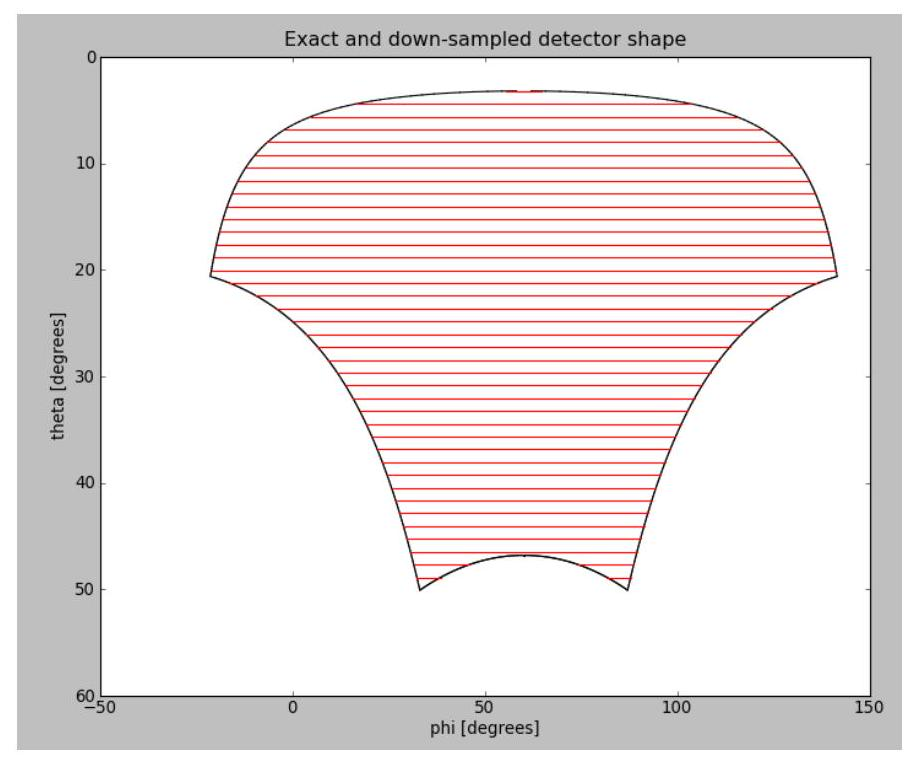
\includegraphics[max width=\textwidth, center]{2025_02_07_204a351db2d7f48b61ebg-190(1)}

Figure 8.4: A rectilinear detector defined by the user in its plane and automatically transformed into the required $\theta(\phi)$ sampling for GOSIA. the desired calculation. Note that the GUI does not interpret gosia.inp files created by the user. Once a gosia.inp file is changed by hand, it is usually necessary to abandon the GUI to continue calculations or fitting. One exception is the error analysis. Correlated error calculations can be run outside of the GUI according to the Gosia manual, allowing more flexibility in the procedure.

\subsection*{8.2 What is new in Rachel 1.0}
Rachel 1.0 includes some new features that greatly facilitate preparation of Gosia input for complicated systems. Refer to the appropriate section in the Rachel manual chapter for more information about these added capabilities of Rachel.

\section*{Ge physical type library (Tigress, MiniBall, Gammasphere.)}
A number of Ge crystal types for standard detector arrays are available in the "standard library" accompanying Rachel 1.0. New detector types can be added to the "user library." Please submit new standard Ge crystal definitions through the Gosia Forums: \href{http://www-user.pas.rochester.edu/~}{http://www-user.pas.rochester.edu/\~{}} gosia/phpBB3/

Fast, simple loading of Ge array definitions (positions)\\
Common Ge array definitions (MiniBall, Gammasphere, Tigress, etc.) are included with this Rachel version. These can be imported and attached to one or more experiments using the button "Attach/delete Ge dets." New array definitions can be typed by the user in a human-readable text format and added to the library. Please submit new definitions of commonly-used detector arrays through the Gosia Forums.

\section*{One-click loading of all experimental data}
In the beta versions, the data file name for each detector in each experiment had to be specified by the user. This meant lots of typing in the GUI or making copies of an array definition file, each with unique file names. Now, loading data files for each detector in all experiments can be done using the systematic file naming system used by Rachel 1.0. This can be done in a single click of the "Import yields" button.

Clearer, more accurate description of the efficiency corrections in simulations.\\
Early beta versions used an "intrinsic efficiency" that was defined as the probability ( $0-1$ ) of a $\gamma-$ ray falling in the photopeak if it was incident on the detector face. This definition was not appropriate for detectors of arbitrary size and at arbitrary distances from the target. In Rachel 1.0 (and late beta versions) the standard measure of $\gamma$-ray efficiency is used and is completely controlled by the user, if the default values are not applicable. Each crystal defined in the "physical" Ge crystal library distributed with version 1.0 has an efficiency curve from an actual calibration run (e.g. Gammasphere, TIGRESS, MiniBall). Note that real experimental data used in Rachel must be corrected for the relative efficiency. (The absolute efficiency is irrelevant in Gosia fits except for cases where the ratio of the $\gamma$-ray yields to elastic scattering is measured, chapter 7.13.) The efficiency curves included in Rachel are used only for simulations in planning experiments.

\section*{Stopping power calculations at the best accuracy possible}
The approximate stopping power and range calculations performed by Rachel as the user defines experiments now use the Oak Ridge code ELAST, which is distributed with Rachel version 1.0. This replaces the ELO (author unknown) calculations used in the beta versions. These stopping power calculations differ significantly from SRIM calculations. Accurate stopping power and exit energy values are important for accurate predictions and fitting of matrix elements. Rachel version 1.0 can make a call to the Rochester SRIM server using the button "Stopping power" to load more accurate values.

\section*{Fast deorientation tensor calculation and lifetime calculation}
The deorientation tensor can be calculated in seconds by running a "Deorientation coeff." calculation. This also produces an accurate calculation of lifetimes, including all decay branches and internal conversion branches.

\section*{Scripting capability (under development)}
The GUI will run scripts written in the Python version in use. This can be used for fitting parameters that Gosia does not include in the $\chi$-squared minimization, iterating calculations automatically, producing output files of data that are not normally written by the GUI, generating file formats for other codes, etc. Simple user-accessors are not available now, but users are encouraged to contact Rochester with scripting questions.

\section*{Automated setup script that compiles gosia, elast, and sets up Rachel.}
A setup script is now included with the Rachel distributions. This script compiles the necessary executables (except gnuplot) and generates the .rachel\_setup file, which can be modified by the user.

\section*{User help}
Popup tips (which can be turned off in the .rachel\_setup file) now follow each user action. These tips suggest the next action to set up calculations and give advice and warnings. A "What's new" video will be available on the Gosia Wiki shortly after the release of version 1.0. The latest version of RACHEL is available at:\\
\href{http://www-user.pas.rochester.edu/~gosia/mediawiki/index.php/Rachel,_a_GUI_for_Gosia}{http://www-user.pas.rochester.edu/\~{}gosia/mediawiki/index.php/Rachel,\_a\_GUI\_for\_Gosia}

\subsection*{8.3 Summary of general features of Rachel}
The following list summarizes the general features available in Rachel.\\
A user-expandable library of standard Ge crystals e.g. Gammasphere for instant setup\\
Fully-automated loading of experimental yield data using systematic file names\\
Partitioning particle-detector data by azimuthal and polar angles\\
Graphical definition of rectilinear or irregular-shaped particle detectors\\
$4 \pi$ experiments (e.g. experiments with no particle detection)\\
Normal or inverse kinematics experiments\\
Data from summed $4 \pi$ Ge arrays\\
Data from pre-defined or user-defined Ge arrays\\
Partitioning of gamma-ray yields into summed clusters e.g. GRETA modules\\
Efficiency-corrected gamma-ray data only\\
Experiment planning aids: Generation of simulated data based on a proposed beam run with counts calculated using absolute efficiency; Optional quasi-Gaussian random scatter in simulated data; Estimated precision of the proposed measurement ( $\mathrm{B}(\mathcal{M} \lambda)$ or matrix elements).\\
Accuracy testing to determine if Gosia will be appropriate for a planned experiment\\
Fitting and correlated error estimations\\
Reading level schemes and gamma-ray data from Radware AGS or user-readable text files and including: Branching ratio data; Previously measured EM matrix elements, including the measured phases; Lifetime data for excited states (not the ground state lifetime); Mixing ratios\\
Several supported data file formats: Radware AGS format; Rachel format nuclear data files; Gosia format (experimental yield and fitted matrix element data)\\
Instantly generating plots of experimental vs. predicted yields via gnuplot\\
Automated generation of stopping power and internal conversion input for Gosia\\
SRIM stopping power lookup via the Rochester SRIM server\\
Push-button controls\\
A searchable help function\\
Saving the entire session to a file\\
Undo/Redo of most functions and crash recovery

\subsection*{8.4 The code}
RAChel is written entirely in Python with calls to Gosia and elast (The Oak Ridge stopping power code). Rather than passing data in and out of these two codes, the GUI calls the codes and then parses the output files generated by them. Version 1.0 can also call the Rochester SRIM server for more accurate stopping power data. (Chapter 5.3 illustrates the $10-15 \%$ discrepancy between SRIM and other codes or compilations.)

The Clebsch-Gordan coefficients function was translated into Python from the Fortran function NED [NED03]. Use the "Help" button, topic "credits" to see all credits.

\subsection*{8.5 Installation}
Refer to section 8.11 for information about specific architectures and operating systems.\\
Install the GUI on the machine where GOSIA will be run in a new directory by simply un-tarring the distribution package. The GUI does not support running GOSIA remotely on a different machine.

Among other benefits, the use of Python allows for portability of the code. The GUI has been run without modification on the following systems: OS X 10.5 and 10.6, Ubuntu version 10.04, SUSE Linux, as\\
well as other Linux/Unix flavors. Currently, the GUI will not run under Windows because it uses a number of Linux-type system calls. There may be graphics problems running under Ubuntu version 11.04 and higher. In the short term, contact Rochester for help resolving graphics problems. An upcoming version will use more portable GTK graphics.

Python version 2.6 is required to run Rachel. It should be Python 2.7 compliant on most machines. The following Python libraries, appropriate for the Python version in use, must be installed:

\begin{center}
\begin{tabular}{lllll}
pickle $^{1}$ & readline & copy & time & math $^{1}$ \\
bisect & numpy & pylab & matplotlib & pyplot (a module of matplotlib) \\
pygtk (version $\left.2 .^{*}\right)$ & gtk & gobject & os & pango \\
sys & subprocess & random ${ }^{1}$ & string & textwrap \\
\end{tabular}
\end{center}

After following the instructions in the remainder of this section, you can test for missing libraries by invoking the GUI. If it reports a missing library, install it by using easy\_install at the system prompt. This is a standard Python auxiliary installer. (If you do not have sudo or root privilege, contact your IT department.) Be sure to use the easy\_install version corresponding to the correct version of Python on systems where a Python version older than 2.6 is also installed. Do not remove the original version of Python from your machine. Other software may depend on this original version.

The .maplotlib/matplotlibrc file in the user's home directory may need to be modified to use the proper graphics back-end for the system. On Linux, TkAgg usually works, but this depends on the configuration of Python. On OS X systems use "macosx". See\\
\href{http://matplotlib.sourceforge.net/faq/installing_faq.html}{http://matplotlib.sourceforge.net/faq/installing\_faq.html}\\
for more information. See chapter 8.11 for more details.\\
In order to use the yield-plotting feature, gnuplot must be installed on the system and located in the user's PATH settings or by link or alias, i.e., gnuplot must be invoked by the command gnuplot at the system prompt on the machine running RACHEL. (Other plot packages may be supported in the future.)

\subsection*{8.5.1 Compiling elast and gosia using the compile-all.sh script}
Move into the directory where the Rachel tar archive was extracted (the location of \href{http://rachel.py}{rachel.py}) and run the \href{http://compile-all.sh}{compile-all.sh} script. This is usually done by typing\\
./compile-all.sh\\
This will compile the Gosia version distributed with Rachel, which is in the gosia\_source directory and the Elast version modified for command-line use by J.M. Allmond, which is in the elast\_source directory.

The compile-all script will also create a .rachel\_setup file in the home directory, which can be copied to another account and/or a working directory. This setup file contains some user settings and the locations of the executables and the BRICC data files. This file can be modified in a text editor, for example to turn the popup tips on or off.\\
./compile-all.sh clean will remove the compiled executables.\\
Thanks to J.M. Allmond for the compiling script.

\subsection*{8.5.2 Compiling elast and gosia without the compile-all.sh script}
Currently, RACHEL requires that ELAST is available for estimating the stopping power for the experimental setup and that the BRICC data files are available for GOSIA.

Compile the versions of elast and GOSIA that come with the GUI package. Since the GUI uses a relatively new GOSIA command OP,INTI, a recent version of GOSIA must be used.

To compile gosia and Elast , use a standard Fortran 77 compiler such as g77 or gfortran.\\[0pt]
Note that the BRICC internal conversion executable is not needed. To obtain a newer version of the BRICC data files, refer to the NNDC website [NNDC].

The GUI requires that all executables and auxiliary files are on the machine where the GUI is to be run. The GUI can be run remotely by piping the XWindows using ssh $-[\mathrm{X} \mid \mathrm{Y}] \ldots$ or similar, but it is not possible in the present version, for example, to run RACHEL on the local machine, calling GOSIA, ELAST, or auxilary BRICC files on a remote machine.

\footnotetext{${ }^{1}$ This library and a number of other libraries in this list come with the standard Python installation.
}\subsection*{8.6 Getting started}
\subsection*{8.6.1 Level scheme}
\section*{Finalize the level scheme}
For an accurate Coulomb excitation calculation, it is important to include one or two states in every sequence or band above the observed transitions. This ensures that the contributions to the population of observed states, due to the decay or virtual excitation of higher-lying levels, will be calculated accurately. Add these "buffer" states before reading the level scheme into RACHEL . The level energies in Rachel must be entered in keV for compatability with Radware and the NNDC compilations. Rachel converts the excitation energies to MeV as required when passing them to Gosia.

Note that the present version of the GUI will become confused if there are two or more states of the same spin in the same "band." (GOSIA does not consider bands, so the separation of states into bands is only for ease of defining the matrix in RACHEL.) It will also cause problems to put states of different parity in the same band. To avoid problems, create as many bands for the GUI as necessary, so that each band has at most one level of each spin and only one parity for all states in the band. The even and odd signatures for a band can be merged in the GUI if this simplifies adding groups of interband matrix elements.

The GUI will assume $K$ values for each "band," but these can be changed as desired using the button "View / set K". GOSIA interprets only reduced matrix elements and does not consider any $K$ value; the $K$ values are used only to compute the matrix element Clebsch-Gordan coefficients when generating a set of matrix elements using a collective model.

\section*{Using Radware}
Choose band names so that they are easy to type and contain no spaces. Radware allows a maximum of eight characters in a band name. Band names for each signature must be unique, unless it is desired to permanently merge them in the GUI.

Once the gls file is finalized, use the Radware utility gls\_conv, option 3, to convert it to an AGS (text) format file that RACHEL can read (below).

The GUI compresses all Radware band names by removing all whitespace. Hence, it is important to choose band names in Radware that do not differ only in whitespace. For example, bands "b 1" and "b1" used in the Radware level scheme would both be compressed to "b1" in the GUI and could cause problems. Also, some of the gls/ags files in the Radware site level scheme library have two states of equal spin or different parity which use the same band name and states with no spin or parity assignment. In order to begin calculations with a level scheme file from the Radware library, these states must be moved to different bands and spin-parity assignments must be made using Radware, before converting to the AGS format for RACHEL.

\section*{Using text files for level data}
An example of a properly formatted Rachel level scheme file follows:

\begin{verbatim}
4189 # The Z and A of a phoney nucleus
gsb 1.5 - 0.0 # the ground state
gamma 3.5 # an incorrectly formatted line will be ignored
gamma 2.5 + 100. # The parity symbol should be separated by a space from spin and energy.
side 5.5 + 250. # Note that all the excition energies are given in keV.
side }7.5+300
side2 9.5 - 350. # Only states of one parity can be in single band.
\end{verbatim}

The band "gsb" has one level, spin 1.5 , parity negative at energy 0.0 keV . This will be automatically assigned band number 1. The band "gamma" will be automatically assigned the next available band number, 2. It has two states, spins 3.5 and 2.5 , but the line for the $I=3.5$ state is incorrectly formatted (missing the parity and energy). This level will not appear in the level scheme. The GUI will be confused by spaces in band names in text-file level schemes.

\section*{Starting rachel}
To start RACHEL make a separate working directory for each new Rachel setup. Type\\[0pt]
python [path]/rachel.py\\
where python may require a path or a version number. On some systems with multiple Python versions, for example, it may be necessary to use python $26 .$. or similar to invoke the correct Python version. Alternatively, the first line in the \href{http://rachel.py}{rachel.py} file\\
\#!/usr/bin/env python2.6\\
can be modified to invoke the desired python environment. In either case, the full path to Rachel must be specified, or the rachel. py executable must be found in the default path, or called by a shell alias. Since the terminal is used for user prompts, Rachel cannot be run "in the background," e.g. with\\[0pt]
python [path]/rachel.py \&

\subsection*{8.6.2 The .rachel\_setup file}
If this is the first time that RACHEL is started, and there is no .rachel\_setup file in the working directory or the user's home directory, then the GUI will issue a warning on startup that it cannot find the .rachel\_setup file, and it will prompt for the necessary information to generate the file in the working directory. It will then write the file, re-read it, test the validity of the paths and executables defined and report any errors. If errors are reported, it will give the option to regenerate the setup file correctly. An example of a correctly formatted .rachel\_setup file follows.

\begin{verbatim}
ELAST_EXECUTABLE = elast
GOSIA_EXECUTABLE = gosia
BRICC_IDX_FILE = /home/schrodinger/programs/bricc/BrIccFOV22.idx
BRICC_ICC_FILE = /home/schrodinger/programs/bricc/BrIccFOV22.icc
RACHEL_DIRECTORY = /home/schrodinger/programs/rachel
MAXIMUMUNDOSTEPS = 30
\end{verbatim}

The final entry is the maximum number of undo steps that the GUI will allow. (There is not a prompt for this entry in the interactive setup.) Do not set the number of undo steps fewer than about 10, because the GUI also uses the "undo" invisibly for accuracy-testing features and for crash recovery. Undo information is stored in external files that are cleaned when quitting or re-starting RACHEL. These files are usually very small. For large, rotational nuclei (e.g. $A \sim 180$ or $A \sim 238$ ), they will usually be no larger than $\sim 200 k B$ each, so setting a large number of undo steps should not use significant disk space.

If the .rachel\_setup file is placed in the user's home directory, then it will not be necessary to generate one in each new working directory. A setup file in the working directory, however, will supersede one in the home directory.

\subsection*{8.6.3 Add the matrix elements}
\begin{enumerate}
  \item This can be done by adding one reduced matrix element at a time using the button "Add $\left\langle I_{f}\|\mathcal{M} \lambda\| I_{i}>\right.$ " after selecting the multipole in the top-right pull-down tab and entering the initial and final band numbers in the "initial / final band " text entries. The GUI will interpret mathematical operations including ClebschGordan coefficients at the prompt that follows.\\
-or-
  \item Rotor model parameters can be entered for matrix elements in a similar way by selecting the multipole and equal initial and final band numbers and the button "Add/change m.e." This will prompt for the appropriate intrinsic moment for inband E2 or M1 matrix elements, which, in this case must be a number, not a mathematical expression. This will add an entire set of inband matrix elements based on the rotor model. M1 static moments are not included, because they consume space in the limited memory of gosia and have insignificant effect on the population cross sections.
\end{enumerate}

Interband matrix elements can be added by either of the methods above. If they are to be entered systematically using method 2 , then before using the "Add/change m.e." button, select a "systematic" from\\
the pull-down tab just above the "Initial / final band" entries. Individual matrix elements or sets of matrix elements can be selected as fit parameters, to allow GOSIA to deviate from these initial guesses of systematics.

To add nominally $K$-forbidden interband matrix elements, either change the $K$ values of bands as desired before adding matrix elements, or use the rule " $K$ forbidden" in the systematic pull-down tab. This uses the systematics of equation 4.95 in [BOH69].

\subsection*{8.6.4 Experiments}
Refer to the GOSIA manual for a definition of an "experiment." In short, it can refer to a unique laboratory experiment, to a partition of the projectile or target scattering angles, or to an individual particle detector. Experiments can be added or deleted with the button "Add/delete expt," which prompts the user for all necessary information to define the experiment.

The GUI button "Examine setup" has an option "Experimental setup," which will print a catalog of the following form:

Experiment catalog

\begin{center}
\begin{tabular}{llllll}
------------------------------------------------------ &  &  &  &  &  \\
\# & 1 & 2 & 3 & 4 & 5 \\
theta\_min & 25.0 & 34.0 & 43.0 & 35.0 & 24.0 \\
theta\_max & 34.0 & 43.0 & 52.0 & 50.0 & 31.0 \\
un-inv. Z & 54 & 54 & 54 & 82 & 82 \\
un-inv. A & 136 & 136 & 136 & 208 & 208 \\
Ebeam & 650.0 & 650.0 & 650.0 & 985.0 & 985.0 \\
Norm to expt \# 1 & 1 & 1 & 4 & 4 &  \\
\end{tabular}
\end{center}

In the example above, experimental yield data for experiments 2 and 3 will be interpreted by GOSIA and the GUI as normalized to the data of experiment 1 , and similarly, experiment 5 is normalized to experiment 4. Generally, normalizing one data partition to another for the same beam run experiment will greatly increase the sensitivity of the fit of the matrix elements to the data, so it should be attempted wherever possible. It is not likely that two different laboratory experiments can be normalized one to the other, since generally the different beam doses have not been measured and taken into account in normalizing the yield data from each.

Do not attempt to "chain" the normalizations of experiments. There should be only one normalizing experiment within a subset of experiments. For example, in most cases the GUI will refuse to allow experiment 3 to be normalized to experiment 2 if experiment 2 is normalized to experiment 1 . The following example is not valid.

\begin{verbatim}
Experiment catalog
\end{verbatim}

\begin{center}
\begin{tabular}{llllll}
----------------------------------------------------- &  &  &  &  &  \\
\# & 1 & 2 & 3 & 4 & 5 \\
theta\_min & 25.0 & 34.0 & 43.0 & 35.0 & 24.0 \\
theta\_max & 34.0 & 43.0 & 52.0 & 50.0 & 31.0 \\
un-inv. Z & 54 & 54 & 54 & 82 & 82 \\
un-inv. A & 136 & 136 & 136 & 208 & 208 \\
Ebeam & 650.0 & 650.0 & 650.0 & 985.0 & 985.0 \\
Norm to expt \# 1 & 1 & 2 & 4 & 4 &  \\
\end{tabular}
\end{center}

The normalizations for logical experiments $1-3$ are "chained": experiment 3 is normalized to experiment 2 , and experiment 2 is then normalized to experiment 1 . This could cause inaccuracy in fitting matrix elements to experimental yield data.

\subsection*{8.6.5 Yield data}
To make Coulex simulations, including the generation of simulated data to test the uncertainties for a planned experiment, skip this section. In that case, only one level scheme file is needed.

Each data set corresponds to one laboratory ("logical") detector in one logical experiment. (See the GOSIA manual for the definition of a "logical experiment.") A detector can be defined as a $4 \pi$ array in\\
the GUI. For more than one (logical) detector or more than one experiment (the majority of cases), the experimental yields for each detector must reside in a separate AGS or text file. AGS files contain both the level definitions and the intensities, while Rachel-format text files keep the level scheme in one file and the yield data in one or more separate files.

When the GUI writes yield data for GOSIA, it will not include data for states which cannot be populated and which cannot decay according to the current matrix definitions. This will save space in the limited array sizes of GOSIA.

\section*{Using Radware ags files for yield data}
When using Radware programs gls, escl8r or levit8r to record the yield data, make sure that the overall normalization will allow all experimental yields to be represented accurately within the precision of the gls/ags file output. These files round intensities to $10^{-4}$, so the yield and error should be represented accurately within this precision. Only relative yield intensities are considered in GOSIA, the overall normalization being adjusted as a fit parameter. Naturally, if the $\gamma$-ray yield data for one GOSIA logical experiment are normalized to that of another logical experiment, then the yields for these experiments must use the same normalization.

One AGS file is required for each GOSIA data set (one per Ge detector for each logical experiment) in Rachel, since each GLS or AGS file represents the data from one detector. Use the Radware "edit gamma" function (EG) to give the measured intensity by hand if the intensities were not fit using escl8r or levit8r.

Convert the gls file to an ags (ascii gated level scheme) file using option 3 in Radware gls\_conv:

\begin{verbatim}
$ gls_conv
\end{verbatim}

\begin{verbatim}
GLS_conv Version 2.0 D. C. Radford Sept 1999
    Welcome....
\end{verbatim}

Type 1 to create a level scheme figure in postscript\\
from a .gls file,\\
2 to output level and gamma data (.dat file) from a .gls file,\\
3 to convert a .gls file to an ASCII (.ags) file,\\
4 to convert an ASCII .ags file to a .gls file,\\
5 to calculate $B(M 1) / B(E 2), B(E 2) / B(E 2)$ and $B(E 1) / B(E 2)$ ratios,\\
or 6 to calculate $E($ band1) $-E(b a n d 2)$ or $E$ - RigidRotor\\
energy differences.\\
. . . Response $=$ ? 3

If transitions have no yield data for a particular data set (.ags file), the arrows representing these transitions should either be deleted or toggled to "tentative" dashed arrows, so that their Radware default intensities will be ignored by the GUI.

\section*{Using text files for yield data}
Any overall scale for the yield data in text file format is acceptable, within the machine precision, unlike in the Radware .ags file method.

An example of a properly formatted yield data file for one detector follows.

\begin{verbatim}
gamma 2.5 gsb 1.5 1.0 0.1
side 9.5 side 7.5 .5 . 05
side 7.5 side 5.5 .4 . 04
side 9.5 side 5.5 . . . 03
side 5.5 gamma 2.5 . 2 . 02
\end{verbatim}

The yield of the transition from band "gamma", spin 2.5 to band "gsb", spin 1.5 is $1.0 \pm 0.1$, etc. Obviously, these band names must be identical to the band names in the AGS or text-file used to generate the level scheme. If bands are merged in the GUI, it is not necessary to edit this yield file; the GUI will remember the original band names and assign the yields to the proper states.

\subsection*{8.6.6 Nuclear data}
Here, the term "nuclear data" means only those quantities that are intrinsic to the excited states' decays, i.e., ( $\gamma$-ray) branching ratios, E2/M1 mixing ratios, lifetimes and measured matrix elements (phase sensitive). All nuclear data should be entered into the rachel\_nuclear\_data.txt file, which is in a "human-readable" format as of Rachel version 2.0.0.beta. Refer to the example rachel\_nuclear\_data.txt.EXAMPLE included in the RACHEL distribution. It is best to use the original band names (with whitespaces removed) for separate signatures, so that the branching ratios will be understood if the signatures are not merged in the GUI session. If bands are merged in the GUI, then either the original signature name, or the final name of the merged band may be used to identify the states in the branching ratio data. (It is not necessary in that case to rework the file.)

An example of a properly formatted rachel\_nuclear\_data.txt file is given below.

\begin{verbatim}
# This is an example file. Data are meaningless!
lifetime gsb 2.0 400. 80. # in picoseconds
< gsb 2.0 || E2 || gsb 0.0 > = 2.17 0.02 # Sign is interpreted as positive [eb]
mixing gam 2.0 gsb 2.0 0.35 0.05 # any user comment
< gamod 3.0 || E2 || gsb 4.0 > = -0.45 0.12 # Sign is interpreted as negative
< gsb 2.0 || E2 || gamod 3.0 > = 0.23 0.08 # BACKWARD--WILL BE TIME-REVERSED!*
branching gam 8.0 gamod 7.0 gsb 6.0 0.042 0.005 # gamma-decay branches only, not conversion
#branching band3 3.5 band1 1.5 band1 2.5 0.04 0.01 # This line is commented out
lifetime gam 2.0 5. 2. # cite Jane Doe, PRC 5, 289 (1994)
\end{verbatim}

*Note that time-reversal is done automatically for a consistent phase convention when passing nuclear data to Gosia.\\
Refer to the GOSIA manual for more information and mathematical definitions of these four types of observables, units, etc.

If the nuclear data file exists in the working directory, then the GUI will automatically read and select all applicable data from this file, storing but not passing to Gosia data that pertain to decoupled or missing states. This data collection is done at each fit or error-calculation step, and the file may be modified between successive steps. A "\#" symbol in the first column will "comment-out" (de-select) that line.

\subsection*{8.7 Recommended order of operations}
The order of operations described below will result in the most accurate calculations. In some cases, skipping steps could result in an incorrect interpretation of the results. For example, the calculated ("integrated") yields are not updated by the fitting or correlated error calculation and must be re-calculated after any step that changes the matrix or experimental parameters. Suggestions are printed in the terminal window (or optional pop-ups) before and after running most processes to ensure that the user does not skip an important step, such as re-writing the gosia.yld file after importing new data. Refer to Figures 8.6, 8.7, and 8.8 for the best sequence of operations.

\subsection*{8.7.1 Set up the level scheme}
Make a working directory and copy the level scheme file and any $\gamma$-ray yield data files (one for each detector per experiment) into it. Note that the level schemes do not need to be identical in each yield data file, but band names must be consistent. If fits are not going to be done on data, such as in experiment planning, then only one level scheme file is necessary. If Radware AGS files are used, the $\gamma$-ray yields will be ignored when reading only the level scheme. In the working directory, start RACHEL (section 8.4).

Once the GUI control panel is displayed, the level scheme can be read. Click "Read level scheme" on the control panel, and answer the prompts for the type, AGS or plain text, and file name in the terminal window. (Remember that only the AGS ascii version can be used. The GUI will not read GLS files.) Enter the mass number of the nucleus if the prompt appears for it in the terminal window.

The following order of setup is recommended.\\
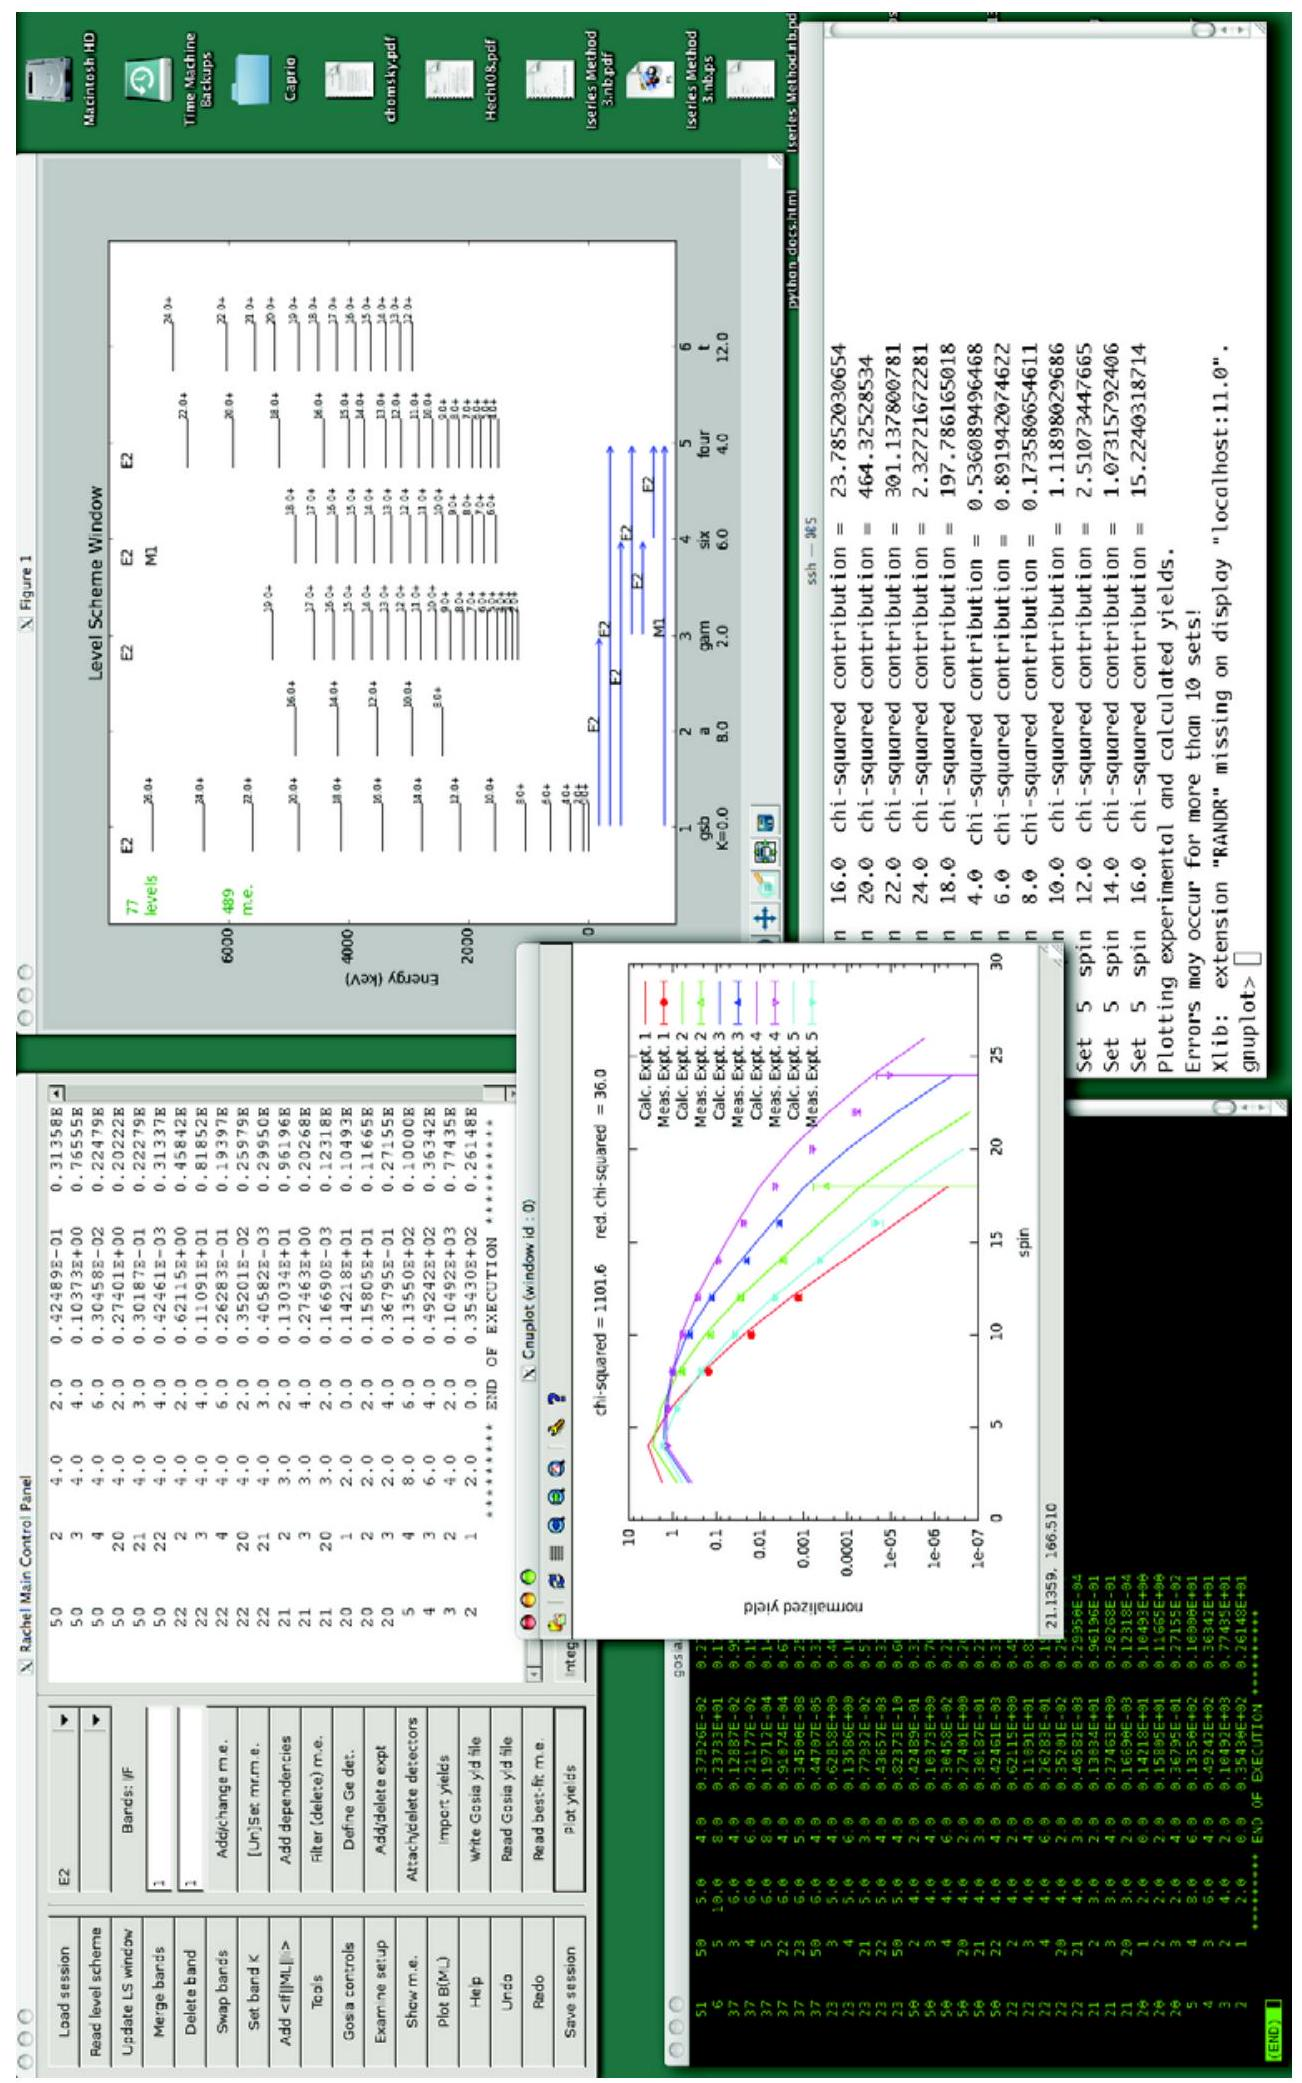
\includegraphics[max width=\textwidth, center]{2025_02_07_204a351db2d7f48b61ebg-199}

Figure 8.5: The main windows of the GUI. At the top-left is the main control panel. At top-right, the level scheme is displayed, including all EM couplings in memory. The terminal window used to start RACHEL is shown at the bottom-right. In the present version, all prompts for the user will be answered in this terminal window. The progress of a calculation can be monitored using "tail -f gosia.out" on Linux-type systems in a second terminal window, shown at the bottom-left.

\section*{Delete unwanted bands.}
Bands can be deleted at any time during a RACHEL session. In version 1.0, if there are experimental or calculated yields in memory, and a band is deleted, it is not necessary to reload any experimental data.

The total number of levels in memory is displayed at the top-left of the level scheme. If there are more than 99 levels, some bands must be deleted, or individual levels must be deleted from the original level scheme file(s). In the latter case, one or more bands should be deleted from memory, and the level scheme should be re-read.

Weakly populated bands or decoupled bands that are not necessary for the calculations can be deleted to save space and simplify the display in an initial fit of the matrix elements of the strongly-populated states for a large level scheme. Bands can be left in the level scheme if their levels have no interband matrix elements that can populate them. In this case, yield and nuclear data for these bands will be automatically left out of the data set sent to GOSIA. If a change is made to the level scheme or matrix, the gosia.yld file should be written again using the button "Write gosia yld file." The gosia.yld file is not written automatically so that it can be edited by hand if desired, but this is not recommended.

To delete a band, click the "Delete band" button and enter band numbers one at a time. Press "enter" to quit.

\section*{Merge bands if desired}
Bands may be merged at any time in version 1.0. Usually, this would be done to merge the even and odd signatures of a rotational band. In many cases, it will be much easier to enter the EM matrix elements systematically, if both signatures are combined, but this is not required.

Enter the initial band number into the first text-entry below "Initial / final band". This will be merged into the band whose number is entered in the second text-entry, and the name of the final band will be kept. Click "Merge bands."

The GUI automatically makes the required phase changes to matrix elements when merging bands.

\section*{Change the ordering of the bands as desired.}
Note: Band 1 must be the GSB, so that GOSIA will understand which is the initial state of the nucleus before the collision. To change the ordering of bands, enter the band numbers to be interchanged in the "Initial / final band" text entry fields and click "Swap bands." The GUI automatically makes the required phase changes when swapping bands.

\subsection*{8.7.2 Add matrix elements}
Be sure to follow a consistent phase convention and add all matrix elements in the upward direction (lower-to-higher energy) in a band and from a lower-numbered band to a higher-numbered band. Note that this differs from the GOSIA input where the order of the input matrix elements must be with index $1<$ index 2 , that is, in the upper right triangle. As discussed in chapters 7.16 and 7.17 , a consistent phase convention is essential to avoid errors due to unintended interference effects. The GUI will automatically correct any matrix elements for time-reversal as necessary, but the user must of course enter a phase that is correct for the direction in which it is entered.

Enter the initial and final band numbers in the "Initial / final band" text entries first. The initial and final band numbers can of course be the same for in-band transitions and static moments.

For large level schemes with rotational band structure, the button "Add/change m.e." can be used to enter a set of matrix elements in one step. If the matrix elements are in-band, then the rotor model will be used by the GUI to generate the set of matrix elements. For $M 1$ transitions, static moments are not included, since they do not have any significant influence on the population probability. (GOSIA assumes one common $g$-factor for all states in calculating the deorientation effect.)

In addition, there is a tool (option "ka" in the Tools button menu) that adds all K-allowed matrix elements to the level scheme using the user's estimates of E2, M1 strengths, etc.

If a set of interband matrix elements is added using the "Add/change m.e." button, then a rule must be selected in the second pull-down tab in the right column of buttons. Currently, as described in chapter 2.4.3, there are three choices: Alaga rule, Mikhailov rule (for rotational-vibrational coupling, e.g. for coupling\\
the ground-state band to the $\gamma$-vibrational band) and K-forbidden, which assumes Bohr and Mottelson's treatment of K-forbidden transitions [BOH69].

Follow the prompts to add matrix elements. After they are added, they can be viewed by clicking the "Show m.e." button at the left. The $B(M \lambda)$ values can be plotted in the level scheme window by clicking "Plot $\mathrm{B}(\mathrm{ML})$." The reduced transition probabilities are plotted with units of $e, b, \mu_{N}$ in the excitation direction (low-energy to high-energy and left to right) to follow the convention used by GOSIA, but the Weisskopf unit is displayed as a red dashed line in the traditional downward direction.

Matrix elements can be deleted with the "Filter (delete) m.e." button by entering Boolean rules according to the instructions in the terminal window. The "Undo" button can be used to revert to the previous matrix.

The "Update LS window" will show which bands have been coupled and which have in-band matrix elements. In both cases, one or more matrix elements define a "coupling." Alternatively, choose the multipole and initial/final band numbers and click "Show m.e." to see each reduced matrix element defined by an arrow indicating the correct direction to be passed to Gosia.

\subsection*{8.7.3 Select fit parameters}
To fit matrix elements to data, fit parameters may be set as individual matrix elements ("masters"), and optionally other matrix elements ("dependents") may be coupled to them. The dependents will vary in proportion to the masters. There are no restrictions on which matrix elements can be coupled to which masters, except that dependents must always be coupled to a master. Never "chain" the couplings by coupling dependents to other dependents. This is not allowed by Gosia and the GUI should always refuse to allow it.

To add master and dependent matrix elements, select one of the options from the "Fit parameters" menu. Option "s" is used to set an individual master matrix element. Follow the prompts to define the master.

To add the dependents, either answer "yes" to the prompt after adding a master, or choose option "d," from the menu later. Follow the instructions for selecting the master again and enter the Boolean rules to select the dependents. Note that in Python the Boolean equality operator is " $==$, , not " $=$." Be careful to define the Boolean rules selectively enough that you do not make unintended couplings. After adding the dependencies, the master and dependent definitions can be displayed for each separate parameter by clicking "Examine setup" and selecting option "p." Each master will be shown in green on the level scheme, and all of its dependents will be shown in red.

Using Boolean rules allows the most flexibility. Every rule is added using a logical "and" to the preceding rule. Below are some examples.

\section*{Specifying all matrix elements coupling band 1 to band 2}
\begin{verbatim}
Enter rules to define the matrix elements dependent on this master.
    Use the variables ib (initial band number)
            fb (final band number)
            ii (initial spin)
            fi (final spin)
            ml (multipole--same codes as for the master definition above)
    and the boolean operators ==, <, >, not, and, or.
    Expressions on separate lines will be combined by a logical 'and'.
    For example, entering "ib==1 and fb==2 and ml==7" will specify all
        M1 matrix elements coupling band 1 to band 2 as dependent on the
        master matrix element specified above.
    IF YOU MAKE A MISTAKE, ENTER "False" (without quotes, case sensitive)
        on a separate line. This will cancel the operation.
Enter 'q' to quit when all rules are entered:
Rule>ib==1 and fb==2
Rule>q
\end{verbatim}

Specify as dependents only the E2 matrix elements coupling band 1 to the even-spin states of band 2

\begin{verbatim}
Rule>ib==1 and fb==2 and (fi % 2) == 0
Rule>ml==2
Rule>q
\end{verbatim}

In this case, the modulus operator $\%$ is used to select transitions with an even-integer final spin "fi."

\section*{Notes on matrix element couplings}
Note that it is not allowed by GOSIA to couple any dependent matrix element to another dependent matrix element. The GUI will refuse to do this and will print an error, if it is attempted. Instead, couple the desired dependent to the master matrix element for this set.

While GOSIA can fit a large number of parameters, it is wise to select the minimum number of master matrix elements possible to obtain the best fit to the desired measurements. Fitting large numbers of masters requires a tremendous amount of data to obtain a unique $\chi^{2}$ minimum and can give misleading results. However, a correlated error calculation should expose this problem by giving very large errors.

Tip: fit the matrix elements coupling to the strongest states first, and then iterate the fit for the weakly populated states by adding more fit parameters in subsequent fits.

\subsection*{8.7.4 Define the germanium crystal types}
Note that this defines the "physical" detectors used, not the "logical" detectors (both as defined in the gosia manual). In short, a physical detector is defined as one type of Ge crystal or a $4 \pi$ array. If an individual crystal is defined, then each geometrically unique detector type used in the data collection must be defined. Two physical detectors must also be specified as unique types if their distances from the target are different.

To define a Ge crystal or $4 \pi$ array type, click "Define Ge det" on the control panel, and answer the prompts for the geometry of the detector. The GUI will display the standard and user-defined types in the library files. The user can choose from these or define a new type at the appropriate prompts.

Complicated arrays with several types of crystals can be defined using a user-readable text file of the following format. All dimensions are in cm .

\begin{verbatim}
somecrystal
description Some type of Ge crystal
distance 20
outer_radius 4
inner_radius .4
length 9
someother
description some other type of Ge crystal
distance 30
outer_radius 3
inner_radius . }
length 10
\end{verbatim}

To read this file, select option "ip" from the Tools button menu. These may be added to the user's library if they are successfully defined. Be sure to use a unique name for each type defined. Once they have been read into the session they may be "attached" to an experiment as described below.

\subsection*{8.7.5 Define the "logical" experiments}
A logical experiment as defined in the GOSIA manual is different from an experiment in the traditional sense of the term. A unique partition of the particle scattering angles, or obviously a different beam/target combination or different beam run will require the addition of a logical experiment.

Click "Add/delete expt," follow the instructions and answer the prompts in the terminal window to define all logical experiments. New experiments can be added at any time during a session.

ELAST is used to estimate the exit-energy from the target and stopping powers automatically when adding experiments, the user may change the stopping power by hand or call the Rochester server for SRIM data. If SRIM is used the exit energy is recalculated using the SRIM stopping powers. The use of the ELAST and SRIM tables limits calculations to $Z \leq 92$. Rachel version 1.0 can make a call to the Rochester SRIM server using the button "Stopping power" to load more accurate values. The user can specify a known target thickness or a known exit energy. For stopped beams, this server call automatically changes the initial specification of target thickness to the calculated range, so that absolute cross sections (in $m b$ ) will be reported correctly in simulations and plots. This version also handles thick target experiments where the backscattered projectiles are detected from collisions near the surface of a thick target. In this case, the user can calculate (outside of the GUI) the energy threshold for which backscatters are detected, and the GUI can recalculate stopping power data for this range.

Tips:

\begin{enumerate}
  \item Coupling one logical experiment to another for the same beam run (only) reduces the number of fit parameters which increases the sensitivity of the fitted matrix elements to the data. You can do this at the prompts when adding experiments, and you can change the couplings later by clicking "Gosia controls" and choosing option "n."
  \item The present version of Gosia will not give accurate fit results if you couple any logical experiment with a target-detection experiment; the GUI will force you to leave target-detection experiments self-normalized. Alternatively you can define those experiments with the equivalent beam scattering range defined, if this can be done accurately.
  \item Separate particle detectors must be defined as additional experiments, with the exception of PIN diode arrays, which are not yet handled by the GUI.
\end{enumerate}

\subsection*{8.7.6 Attach Ge detectors}
Note that for simulations, Ge detectors can overlap in space. For example this can be used to compare the count rate for a $4 \pi$ array and a single detector.

After defining all of the logical experiments for different beam runs or partitions of the full data set, input the germanium detector positions used for each experiment. (These are defined in the gosia manual as "logical detectors"). That is, they may be of the same "physical detector" type defined above, but each at a unique laboratory $\theta, \phi$ position. This can be done in either of two ways.

For few-detector arrays or $4 \pi$ arrays, click "Attach/delete detectors." If the same type and position of a Ge detector is used for all logical experiments, then the Ge detector can be attached to all experiments at once, following the prompts.

Any arbitrary spherical-polar coordinate system can be used, as long as it is consistent between the particle scattering angles and the Ge detector angles, and the polar angles of detectors are consistent with the beam direction at the polar angle $\theta_{\text {lab }} \equiv 0$.

During this procedure, you can specify a data file (AGS or TXT) to load data "automatically." Autoloading is done using the "al" option in the Tools button menu. If the auto-load feature is to be used, the logical detector should only be attached to one experiment at a time!

The simplest way to load data is to use the fully-automated system. Refer to section 8.7.7. To use the completely-automated data loading, it is not necessary to specify file names in this step.

Tip: If a detector's type is a $4 \pi$ array, you can add it at any polar and azimuthal angle you choose, so for convenience in answering future prompts, you should choose both polar and azimuthal angles as 0 degrees when attaching that logical Ge detector.

For many-detector arrays, a human-readable text file can be used to define the entire array at once. This can be done as arbitrary summed clusters in the array, as single crystals, or as an entire summed array. In each case, the $\gamma$-ray yield data must be partitioned in the same way.

Examples of these detector array definition files are in the .../rachel/detector\_libraries/ directory. The general format is best illustrated by the following examples, and more can be found on the Gosia Wiki.

\begin{verbatim}
# An array of 4 Ge crystals, each with a data file to auto-load.
crystal Crystal01 45. 90. txt yields_expt_1_crystal_1.txt
crystal Crystal01 60. 90. txt yields_expt_1_crystal_2.txt
crystal Crystal01 90. 90. txt yields_expt_1_crystal_3.txt
crystal Crystal01 120. 90. txt yields_expt_1_crystal_4.txt
\end{verbatim}

The example above can be understood as a single crystal ("crystal" instead of a summed cluster "cluster") of type Crystal01 at $\theta=45$ degrees and $\phi=90$ degrees. If this file is read into only one experiment, the GUI will know that the yield data files are in the Rachel text file format (above). The first crystal's data can be auto-loaded from the file yields\_expt\_1\_crystal\_1.txt.

If this file is to be attached to more than one experiment, the GUI needs a separate file for each experiment with the corresponding yield file names, and these should be read separately for each experiment. For example, this file would be read into experiment 1 by clicking Tools and answering the prompts as below.

\begin{verbatim}
[Tools button menu displayed]
Enter two-letter code: id
Enter Rachel detector file name: myarray.txt
Note that if auto-load file names are specified in the
detector array file, a separate file must be used for each
experiment, with unique Ge detector data files for each
experiment.
Enter a list of experiment numbers to add this array to,
    e.g. 1,2,4,7
    Experiment numbers [or "all" or "q" to quit]: 1
\end{verbatim}

This procedure would be repeated for subsequent experiments by modifying only the data file names:

\begin{verbatim}
crystal Crystal01 45. 90. txt yields_expt_2_crystal_1.txt
\end{verbatim}

Any combination of text and Radware AGS files can be used for the yield data.

\begin{verbatim}
crystal Crystal01 45. 90. ags first_set.ags
\end{verbatim}

...

A combination of single-crystals and summed clusters could be entered as follows. This may be most useful for simulations where the different partitionings of data are being tested.

\begin{verbatim}
# Definition of a crystal and cluster combination
# First is a single crystal of type "mytype".
# The first cluster has 7 Ge crystals, while the second has 6.
# The data set for a cluster represents the summed yields of all crystals in a cluster.
crystal mytype 37. 95. txt experiment_1_crystal_1_yields.txt
# cluster number 1
cluster 7 ags experiment_1_cluster_1_yields.ags # This will auto-load from a Radware AGS file.
Crystal03 58.28 72.0 # Comments can be given at the end of any line.
Crystal03 69.82 53.51
Crystal03 69.82 90.49
Crystal03 79.19 72.0
Crystal03 90.0 54.0
Crystal03 90.0 90.0
Crystal03 99.29 72.0
# cluster number 2
cluster 6 txt experiment_1_cluster_2_yields.txt # Rachel format yield file.
Crystal01 58.28 144.0
Crystal01 69.82 125.51
Crystal01 69.82 162.49
\end{verbatim}

\begin{center}
\begin{tabular}{lll}
Crystal01 & 79.19 & 144.0 \\
Crystal01 & 90.0 & 126.0 \\
Crystal01 & 90.0 & 162.0 \\
\end{tabular}
\end{center}

In any of these files, if a simulation is to be performed generating test-data (no real data are to be loaded), or if fully-automated system is used (Section 8.7.7) the file can be read into all experiments at once. In this case, the file name and type can be omitted (and will be ignored by the GUI). For example, the file my \_detector\_array.txt could contain

\begin{verbatim}
crystal mytype 37. 95. # No file type or name
# cluster number 1
cluster 3
Crystal03 58.28 72.0 # Comments can be given at the end of any line.
Crystal03 69.82 53.51
Crystal03 69.82 90.49
\end{verbatim}

and be attached to all experiments at once by answering the prompt

\begin{verbatim}
Enter a list of experiment numbers to add this array to,
    e.g. 1,2,4,7
    Experiment numbers [or "all" or "q" to quit]: all
\end{verbatim}

\subsection*{8.7.7 Load experimental yield data}
For experimental planning where real data will not be used, skip this section and read section 8.8 on simulating data and predicted count rates. Using any loading method, RACHEL will store all data from the files, so that changes in the level scheme or matrix do not require reloading data. When the data are passed to Gosia, it will automatically de-select yields that do not apply to the current calculation.

Experimental yield data must be imported from a unique file for each partition of the full data set. That is, for each laboratory Ge detector in each "logical" experiment, you must have a separate file of yield data, either in a Radware AGS file or in a text file in the RACHEL format. See the section 8.6.5 for the options in yield data format.

\section*{Fully automated loading of yield data}
This method of loading $\gamma$-ray yield data, introduced in version 1.0 , is the simplest and fastest. The user can enter yield data in either AGS or Rachel-format TXT files using systematic file naming and load all data with one click.

To use this feature, name the experimental yield data files using the format\\[0pt]
expt\_[name]\textit{det}[number].txt or expt\_[name]\textit{det}[number]. ags,\\
(All files must be of the same type, ags or txt.)\\
where "name" is the user-defined name of each experiment, and "number" is the Ge detector number (single-crystal, cluster of crystals, or a summed $4 \pi$ array). The experiment names must contain only alphanumeric characters and no whitespace. The detector numbers refer to the order in which they were attached. If detector arrays were defined by file (Button "Attach/delete Ge dets," option "id"), then the numbering of detectors follows the order in the detector array file. To check the ordering, use option "pd" under the same button.

To auto-load the yield data using this method, click "Import yields," and select option "fl," FULLY automatic loading of all yield data. The output will look like the following.

\begin{verbatim}
Import from AGS[a] or TXT[t] files [return to quit]? t
Experiment "abc":
Detector # 1 Trying to auto-load from file "expt_abc_det_1.txt".
3 experimental yields read for experiment 1 , detector 1.
Detector # 2 Trying to auto-load from file "expt_abc_det_2.txt".
3 experimental yields read for experiment 1, detector 2.
Detector # 3 Trying to auto-load from file "expt_abc_det_3.txt".
3 experimental yields read for experiment 1 , detector 3.
\end{verbatim}

\begin{verbatim}
Detector # 4 Trying to auto-load from file "expt_abc_det_4.txt".
3 experimental yields read for experiment 1 , detector 4.
Experiment "def":
Detector # 1 Trying to auto-load from file "expt_def_det_1.txt".
3 experimental yields read for experiment 2, detector 1.
Detector # 2 Trying to auto-load from file "expt_def_det_2.txt".
3 experimental yields read for experiment 2, detector 2 .
Experiment "ghi":
Detector # 1 Trying to auto-load from file "expt_ghi_det_1.txt".
3 experimental yields read for experiment 3, detector 1.
Detector # 2 Trying to auto-load from file "expt_ghi_det_2.txt".
3 experimental yields read for experiment 3, detector 2 .
Done.
\end{verbatim}

\section*{Auto-loading yield data from user-defined file names}
If the detectors have been attached with auto-loading file names specified, then all data can be loaded into all detectors at once ("auto-loaded") by selecting option "al" from the "Import yields" button menu. Data will be loaded for all experiments and detectors that have been set up to auto-load.

If one or more detectors have not been set up to auto-load, click the button "Import yields," and answer the prompts for file type, experiment number and detector number. Give the file name.

\section*{Passing yield data to Gosia}
After all yield data are imported for all experiments and detectors by any of the methods above, click "Write Gosia yld file" to put the data into the gosia.yld yield file that gosia will read in the first step of fitting. Note: the contents of GOSIA's yield file (gosia.yld) is not automatically updated, so rewrite the GOSIA yield file if new experimental data are loaded; if bands are deleted or swapped; if experiments or detectors are added or removed; or if the matrix is changed. If in doubt, rewrite the file after making changes to the setup.

Experimental data are selected automatically each time they are passed to Gosia through the gosia.yld file, so data in the session which do not apply will be omitted.

\subsection*{8.7.8 Generate the gosia detector file}
The detector file gosia.gdt passes to Gosia the definitions of all Ge detector types (not positions). To make this file, select "Make Ge det file" and "Run gosia input," and click "Go." This will tell GosiA to generate a set of efficiency and angular attenuation coefficients $Q_{\lambda}$ for the Ge detectors in use. This only needs to be done once, if you do not add new detector types or work on a different Rachel session file in the same directory, but if you forget this step, GOSIA may give inaccurate results or quit with an error. (If, for instance, you are using two different physical types of Ge detectors, but you have left the gosia.gdt file in the working directory from a different calculation with only one physical type defined, GOSIA may report inaccurate yields without an error.) This step takes only a few seconds, and the output from GosiA will be displayed in the control panel. After running any Gosia process, scroll up and down in this text box and look at the terminal output to check for error messages. If one or more $4 \pi$ Ge arrays have been defined, the GOSIA detector file will automatically be modified by RACHEL so that these entries in the detector file represent $4 \pi$ arrays, but this is transparent to GOSIA, so there will be no indication of this in the GOSIA output.

If this is the first time you have used the "Go" button for this session, you may be prompted for which transition GOSIA should use to normalize the data. Instructions for this prompt are given in the terminal window.

\subsection*{8.7.9 Fitting chosen parameters to the data}
The fitting process involves several steps, and for each of them, you will have to select the appropriate function in the pull-down tab two spaces to the left of the "Go" button, and "Run gosia input" in the pull-down tab to the left of the "Go" button.\\
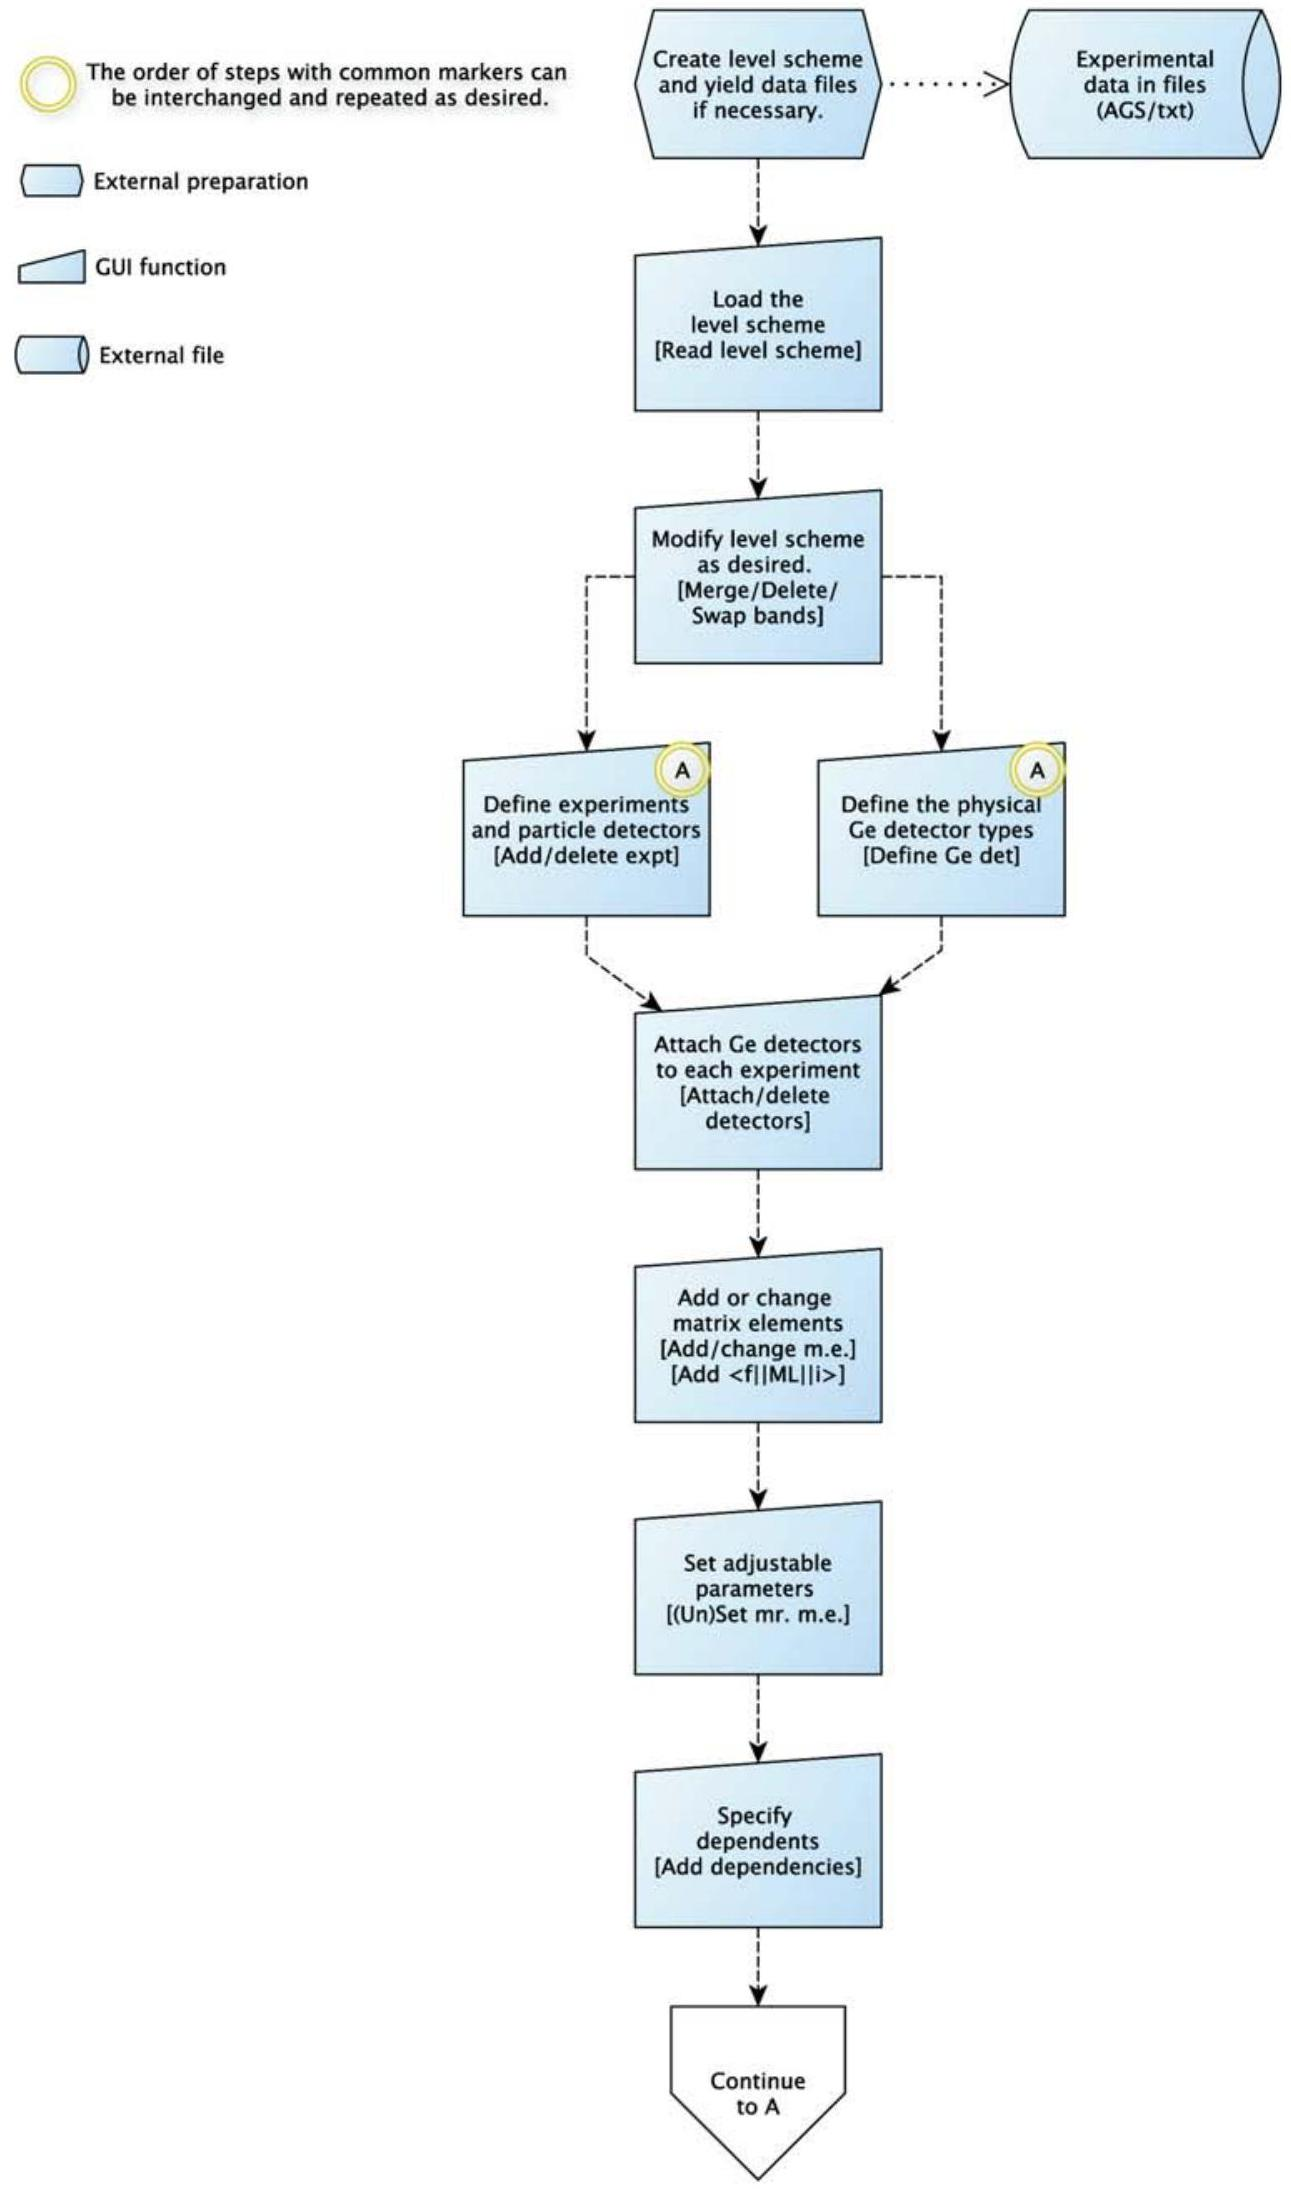
\includegraphics[max width=\textwidth, center]{2025_02_07_204a351db2d7f48b61ebg-207}

Figure 8.6: The correct order of RACHEL operations, part 1.\\
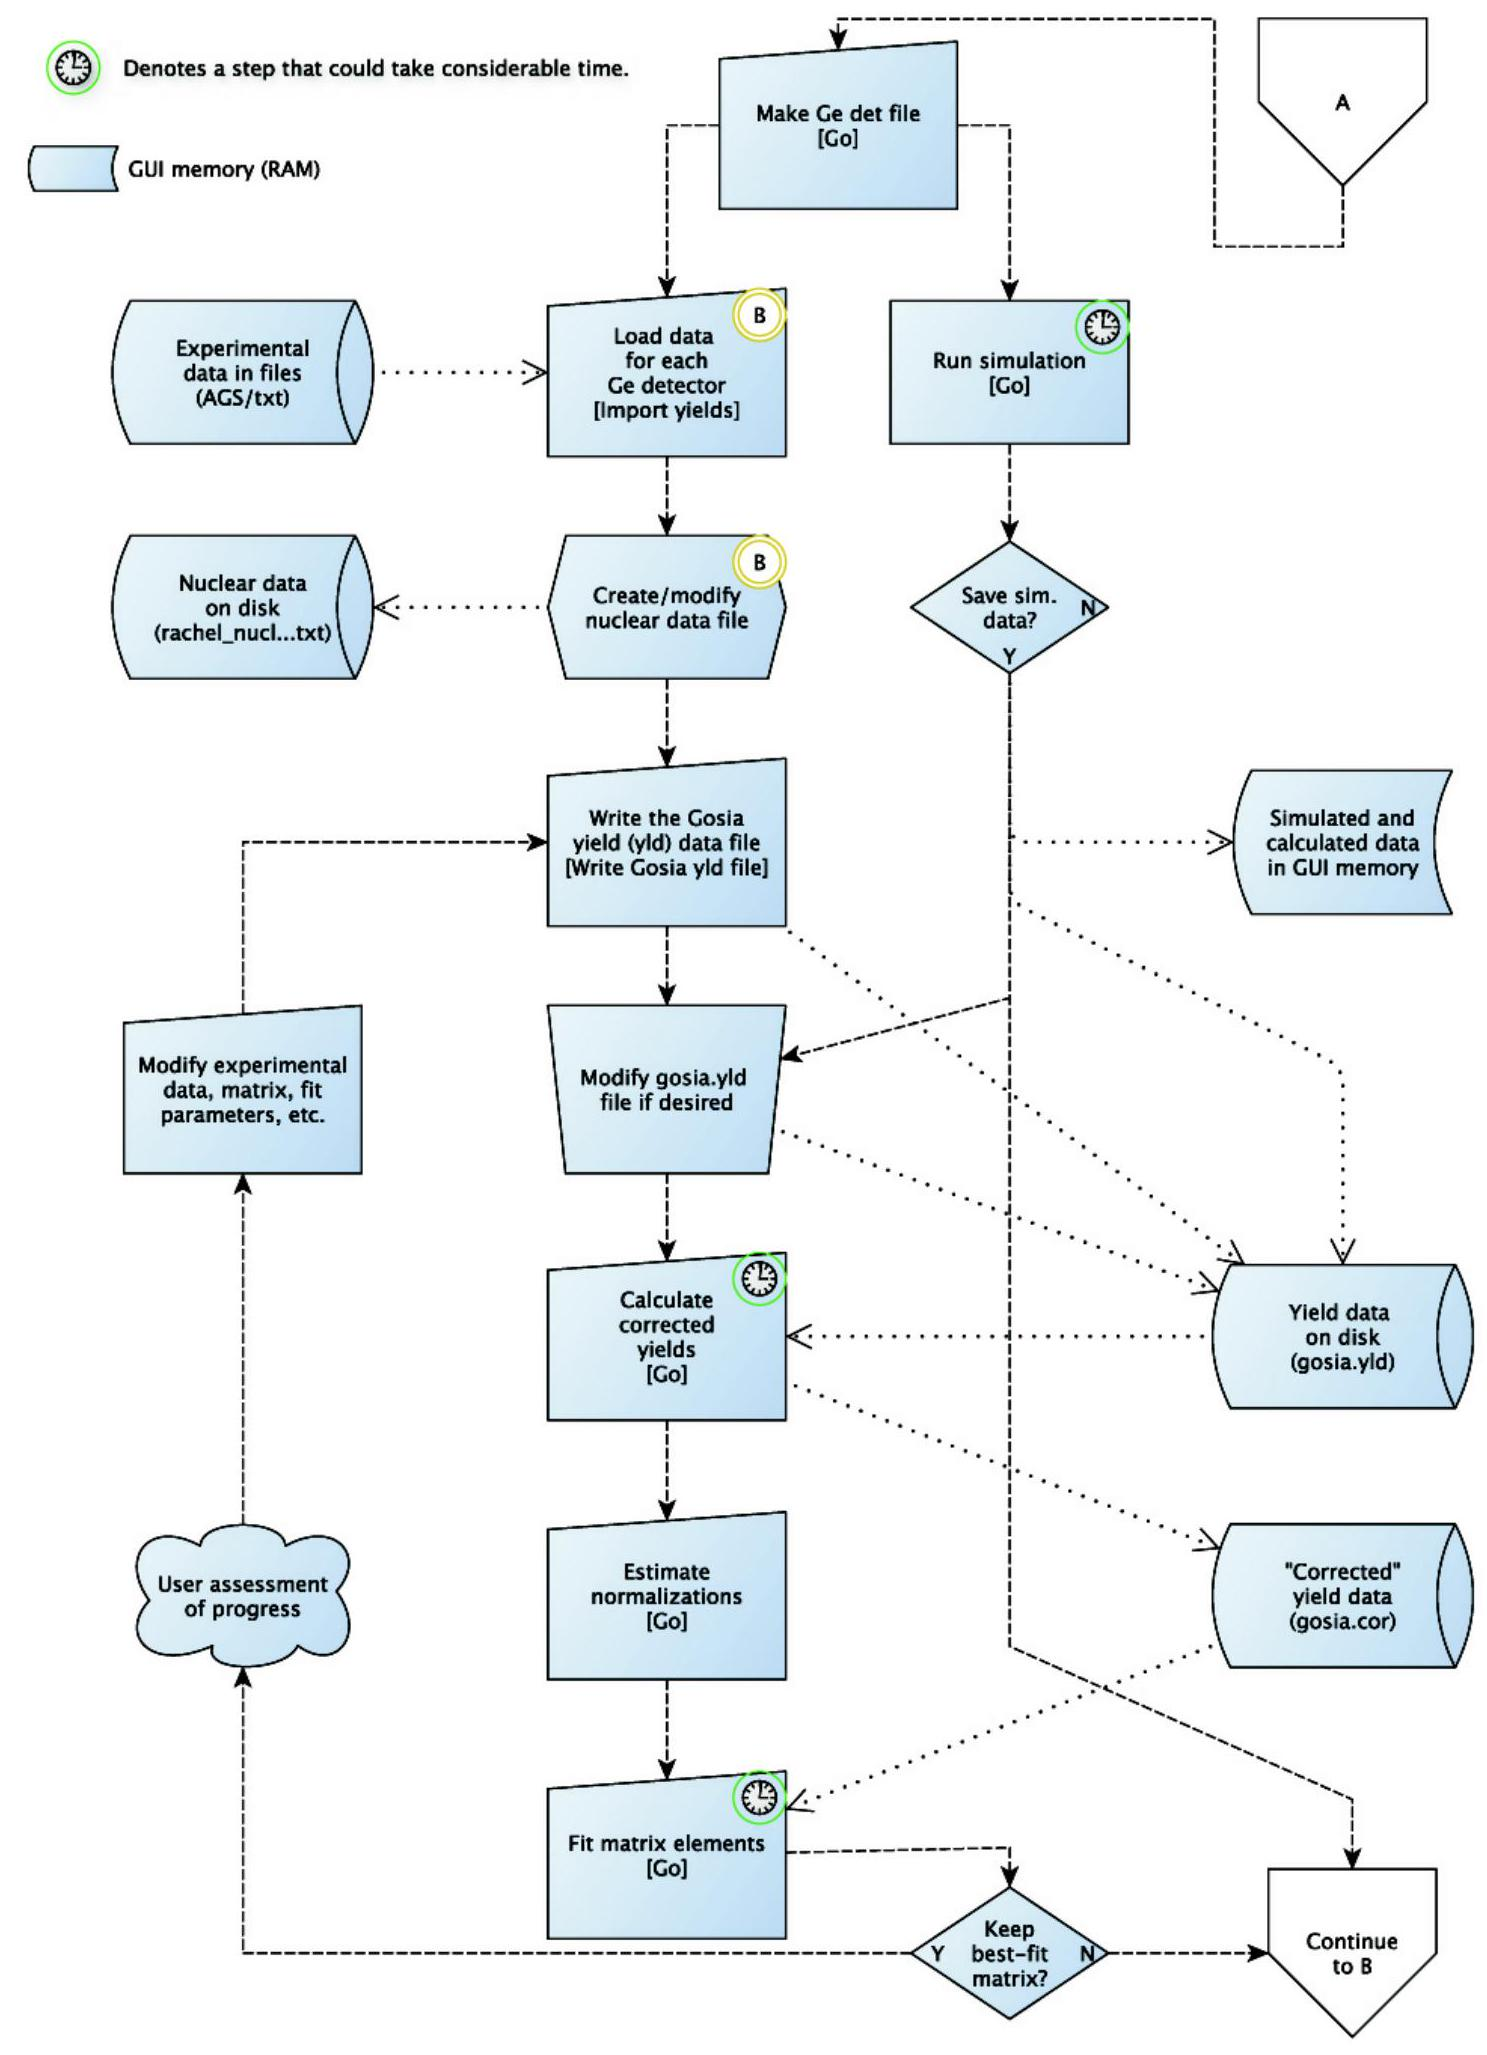
\includegraphics[max width=\textwidth, center]{2025_02_07_204a351db2d7f48b61ebg-208}

Figure 8.7: The correct order of RACHEL operations, part 2. If simulated data are generated, they can be treated as experimental data to obtain predicted errors on measurements.\\
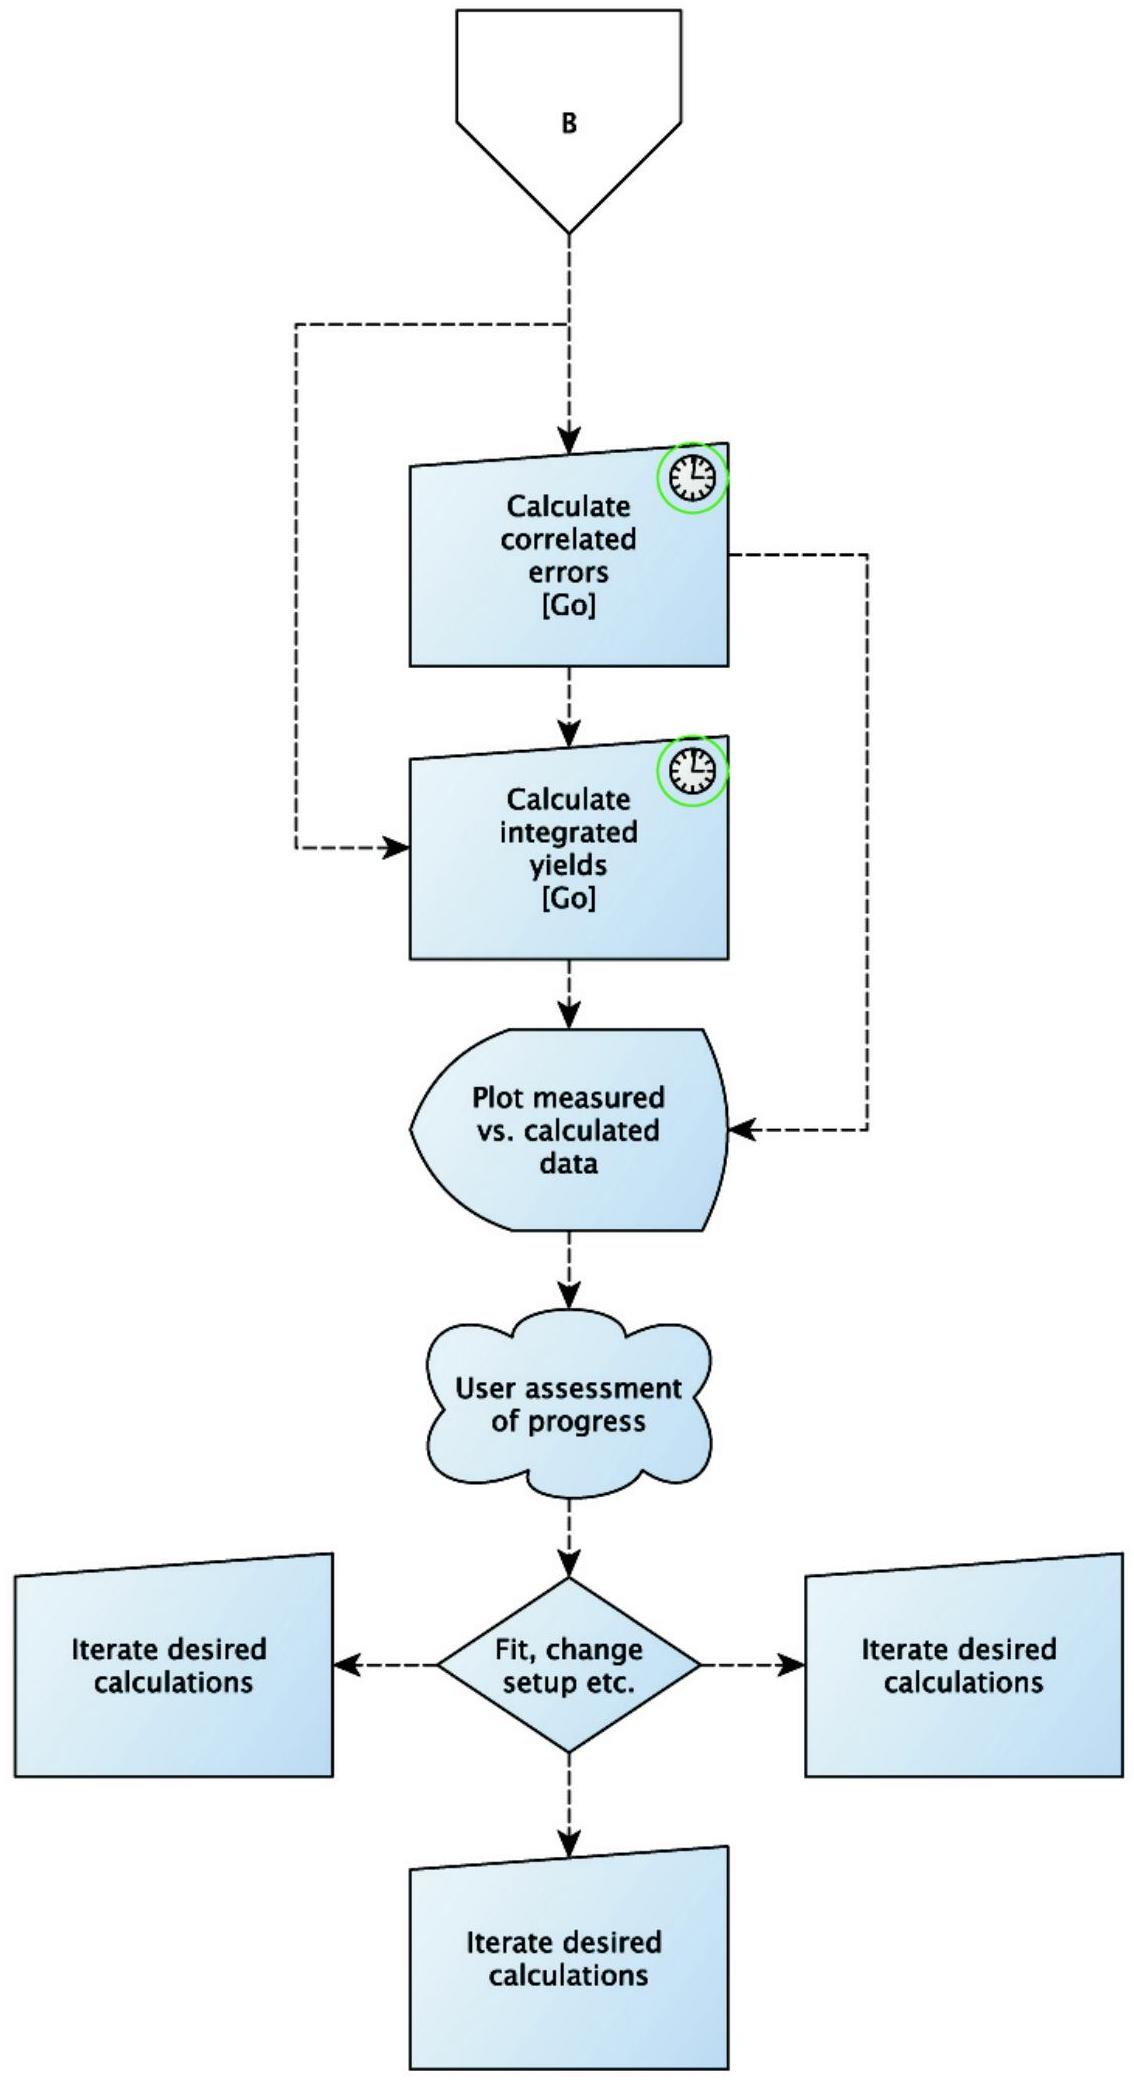
\includegraphics[max width=\textwidth, center]{2025_02_07_204a351db2d7f48b61ebg-209}

Figure 8.8: The correct order of RACHEL operations, part 3. Note that the calculated yields should be integrated any time the experimental setup or matrix is changed, so that plots will reflect the current parameters.

\begin{enumerate}
  \item Make the "corrected yields": This generates from the GOSIA yield data file a set of correction factors so that the point calculations used in the $\chi^{2}$ minimization can be compared to the yields for a range of energy and scattering angle.
  \item Calculate the normalization factors: This generates in the GUI memory a set of factors that GOSIA needs if one logical experiment was coupled to another. You can run this step regardless of the couplings (normalizations "LN") chosen when defining experiments. This operation runs very quickly and does not need to be run again if you do not change or add logical experiments.
  \item Adjust the fitting options(Optional): You can adjust the fitting options by clicking "Gosia controls" and selecting option "f." The options are described briefly at the prompts. Refer to the GOSIA manual for complete descriptions if you need more information. You can change any of these parameters as desired. For example, the default number of fit steps is set initially to 100 . You may want to reduce this number for a first fit, in case the fit does not converge, since 100 steps can take a long time for large level schemes and data sets.
  \item Run a gosia fit. Select "Fit," and click "Go." After the fit, you will have the option to save the new best-fit matrix elements to the GUI memory. Before answering this question, you can view the later sections of the gosia.out file from a separate terminal window to see if any matrix elements have "run away," or were adjusted to the limit at the conclusion of the fit. The latter indicates either that the fit parameter is insensitive to the data, that there is a conflict in the measured data, or that broader limits on the parameter are required. A future version of the GUI will print warnings about these conditions before this prompt. If you intend to iterate the fit starting from the best-fit matrix generated in this step, you will have to answer " y " to this prompt.
\end{enumerate}

\section*{Tips:}
If the reported $\chi$-squared value in the terminal window is "None," or if there are any errors in the GUI or the GOSIA output, do not answer "y" to save the best-fit matrix. In this case, please create a bug report on the Gosia Forum.\\
It is a good idea to monitor the output of the gosia.out file in a second terminal window using tail -f gosia.out or similar. If you get a series of "expansion" errors, the current version of the GUI will not trap these, because it waits for completion of the GOSIA run to analyze the output. If you get these errors, see section 8.9 .8 below. You can press CTRL-C in the RACHEL terminal window since this expansion failure will not yield a fit result.

To check the values of the fit parameters, refer to section 8.5.3 above. You will be able to tell if any parameters did not converge if they are very close to (but not necessarily exactly) their defined limits in the fit results. This could mean that they are insensitive to the data, that you have chosen too many independent parameters, or that your chosen limits for the master matrix elements are too narrow. If you answered "y" to the option to save the best-fit values in the GUI memory, and you now feel that this was a poor choice, you can use the "Undo" button to revert to the former set of matrix elements and then choose different fit parameters, broader limits, different phases of matrix elements, etc.\\
5. Integrate the yields with the best-fit matrix. (You can skip this step and go to step 6 , if you want to iterate the fit immediately. For instance, if the matrix elements have changed in the fit by more than a few percent, you should probably iterate the fitting procedure from step 1, so that GOSIA can attempt to find a best-fit with corrected yields appropriate for the new $\chi$-squared minimum.) Select "Integrated yields," and click "Go." This will generate predicted yields with the best-fit matrix using the full Coulomb-excitation integration over beam energy in the target and scattering/recoil angle for all data sets. Once this step is complete, you can plot the experimental yields against the predictions with the best-fit matrix. See section 8.8 below.\\
6. Iterate the fit. Re-run steps 1,3 and 4 above. It is not necessary to re-calculate the normalization constants, unless the experimental parameters have been changed. Each time you want to plot the results of the fit, you will need to re-run step 5 (integration) before plotting, or you will only see the results of the last integrated predicted yields on the plots, and the $\chi^{2}$ values on the plots will not represent the new fit. Note that running the diagonal error calculation can assist in fine tuning the best solution when close to the minimum.\\
7. Correlated errors: When you have a reasonable reduced $\chi^{2}$, you can run a correlated error analysis by selecting "Correlated errors," and clicking "Go." If you are too far from the minimum, GOSIA may report an inability to perform the error analysis. At the end of the correlated error calculation an improved $\chi^{2}$ may be found, and the matrix at the new minimum can be imported at the prompt that follows. The error estimates will be reported in the terminal window. If a better minimum is reported, you should re-integrate the yields with the newly imported matrix before plotting the data against the predicted yields.

At the conclusion of any of these steps, you may change the matrix, fit parameters, GOSIA controls, etc. If you do so, begin the fitting process again with step 1 . To obtain an accurate plot representing the latest iteration it is always necessary to re-integrate the calculated yields. This is not automated because it can take considerable CPU time in cases with large matrices or many experiments.

Correlated error calculations can be run outside of the GUI according to the Gosia manual, if more flexibility is required. To read the final set of matrix elements following this calculation, Click the "Eval. expression" button and type at the prompt:\\
investigated\_nucleus.parse\_correlated\_errors()\\[0pt]
(The print options in the PRT, block of the Gosia CONT suboption must be the same as those generated by the GUI, and the Gosia output file must contain the results of the final correlated error analysis.) If any of the PRT, options were changed, they can be copy-pasted from the GUI. Select "[Diagonal errors]" and "View gosia input," then click Go. After the diagonal error input is displayed at the end of the textview window, copy-paste the PRT, section to the appropriate place in the input to OP,ERRO. Remember that the correlated error calculation must be run only once following each run of the diagonal errors; otherwise, the correlated errors will be overestimated by about a factor of 2 .

\subsection*{8.8 Experiment planning and testing the ability to measure matrix elements}
Refer to the gOSIA Wiki for a video demonstration of using the "Make simulated yields" function. Simulated data can be generated for experiment planning-for estimating count rates, testing the sensitivity of one or more matrix elements to the predicted yields in your proposed experimental setup (particle detector position, Ge array definition, the most effective data partitioning, etc.) After setting up the experimental and Ge detector definitions for a planned experiment, select "Make simulated yields" in the pull-down tab two spaces to the left of the "Go" button, select "Run gosia input," and click "Go." (Do not forget to generate the Ge detector definition file once for a new session or added Ge detectors.)

The GUI will generate absolute cross-sections from the gosia output, based on your choice of beam, target, target thickness, etc. Following this calculation, you will be prompted for the expected number of days of actual beam time and the expected beam intensity on target. At this time, you will also be able to adjust the efficiency curve(s) and absolute efficiencies of the Ge detectors. The efficiency curve is used only in the simulations. From the calculated cross sections and Ge absolute efficiency curves, observed counts will be calculated for each experiment and detector defined.

The observed counts are then corrected for the estimated absolute efficiency, resulting in data sets of simulated efficiency-corrected data. Errors on the individual yields will be generated based on Poisson statistics, plus the user's answer to a prompt for additional random error, which would typically be at least several percent, but is left to the user to choose. The statistical counting errors are calculated from the predicted observed counts.

\subsection*{8.8.1 Experiment planning}
Optionally, the user can specify a Gaussian scatter at a terminal prompt to be applied to the data, which will result in chi-squared values of $\sim 1$ for the complete data set in test fits. The user can then specify fit parameters, do test fits to the data and error calculations to aid in planning of experiments. (Refer to the sections above.) These error estimates will only be realistic if the random scatter option is chosen.

The user can then test various detector arrangements, partitions of the data by scattering angle (each partition corresponding to one "logical" experiment), beam and target options, etc. to determine the most effective experimental setup for the desired measurements. For example, it is generally found that if there are sufficient statistics to do so, partitioning the full data set into several scattering angle ranges and normalizing\\
these partitions to the first partition greatly increases the sensitivity of matrix elements by providing a probability vs. scattering angle "excitation function."

Test-fits to the simulated data will allow the user to estimate the errors that will be obtained in an actual measurement. Using the fitting procedure above, these errors will include the correlations with other unknowns, which can be difficult to estimate without a simulation.

Some warnings are generated when option "e" in the "Examine setup" button menu is selected if the experimental design exceeds the abilities of GOSIA. In addition, in the "Tools" button menu, there are two test options, "tf" and "ti" that will spot accuracy problems for the proposed experiment. These tests are functional but under development in version 1.0. Explanatory notes are given if problems are found, some of which can be remedied easily, while some may indicate the need for analysis with a full-quantal code. Refer to the demonstration videos for more information [GOS08].

\subsection*{8.8.2 Testing GUI fits}
The user may choose not to apply random scatter. This can be used to generate "perfect" data to test that the GUI is fitting properly, if there is some doubt for an unusual experimental setup. Without the random scatter, a fit should return the sensitive parameters to their initial values, with a final reduced $\chi^{2}$ value of $\ll 1$ after one or two iterations of the fitting procedure described above. If a large value of $\chi$-squared is returned after a few iterations, check that you have followed all steps in the setup and fitting procedures, or repeat them in the order suggested above.

\subsection*{8.9 Plotting}
The plotting function uses gnuplot, which is assumed to be in the user's path environment variable. (If it is not, you can make a symbolic link to gnuplot in the working directory, or an alias.)

Select the initial and final bands in the text-entry fields below "Initial / final band" for which you want to plot yields (the same initial and final bands for in-band yields) and click "Plot yields." You have the option to plot absolute yields (for predictions only) or measured yields, with the chosen normalizations of experiments.\\
(Total Coulomb excitation cross sections can be calculated for $4 \pi$ integration of the $\gamma$-ray emission by attaching a $4 \pi$ detector type to one or more experiments. First, define a 4 pi detector using the Define Ge det. button, then attach it to one or more experiments using the Attach/delete Ge dets. button.)

Once the plot is generated, the Rachel terminal window will be running gnuplot and will accept the usual gnuplot commands, such as those for generating image files of the plot. To resume operation of the GUI and close the gnuplot window, type "q" at the gnuplot> prompt.

Note: The $\chi^{2}$ values reported on the plot refer only to the data set plotted, and the reduced $\chi^{2}$ assumes that the number of free parameters equals the number of data points in the plot. An overall normalization of all experimental data to all calculated data is recalculated each time a plot is made.

Adjustable data set weights are allowed in the GUI, but have not yet been added to the $\chi^{2}$ calculation in the GUI. They are considered in the value given in the Gosia fit output.

\subsection*{8.10 Other tools and functions}
\subsection*{8.10.1 Session recovery after a crash}
The Python GUI rarely crashes. Instead, an untrapped error condition usually results in a traceback report such as the following.

\begin{verbatim}
File "/home/hayes/programs/bin/rachel", line 9274, in gosia_go
    gosia_shell_output = the_gosia_shell.generate(gosia_function,gosia_action)
File "/home/hayes/programs/bin/rachel", line 4293, in generate
    full_gosia_input = self.op_intg_input()
File "/home/hayes/programs/bin/rachel", line 4666, in op_intg_input
    intg_lines = the_experiment_manager.generate_intg()
File "/home/hayes/programs/bin/rachel", line 6120, in generate_intg
\end{verbatim}

\begin{verbatim}
    theta_meshpoints = self.allexperiments[experiment_number].generate_angular_meshpoints()
File "/home/hayes/programs/bin/rachel", line 7867, in generate_angular_meshpoints
    lab_meshpoints,lab_cross_sections = zip(*zipped_list)
ValueError: need more than O values to unpack
\end{verbatim}

The GUI can then be reactivated (button "Reactivate GUI"), but could possibly be in a state that will not allow proper operation. This is rare with the present version. The GUI process can die if it is being run on a remote machine and the connection is terminated, or if the local system crashes.

If a session terminates unexpectedly, it is usually possible to recover the session by restarting RACHEL with the command-line option "-r", i.e. python \href{http://rachel.py}{rachel.py} -r. This will recover the undo data stored on disk. You can examine the setup by generating a GOSIA input, or using the "Examine setup" and "Gosia controls" buttons to determine whether the session was recovered in the state you desire. If it was not, you can use the "Undo" button to revert one or more steps until you are in the desired state, as though the session had not crashed.

If you restart the session without the -r option, it will no longer be possible to recover the lost session, and you will have to revert to the last saved session using the "Load session" button. Also, note that quitting a session with the "Quit" button will remove all undo information from disk and prevent recovery of the session, if you do not choose to save the session upon quitting.

\subsection*{8.10.2 Undo and Redo buttons}
The default maximum number of undo steps is set to 30 , since the undo information is recorded on disk until the user quits the program. The maximum file size for each undo step is $\sim 200 k B$ (much less for small level schemes). This can be changed by adding a line to the .rachel\_setup file:

\section*{MAXIMUMUNDOSTEPS = \#\#\#}
where $\# \# \#$ is the number of undo steps to be remembered during a session.\\
Once the maximum number of undo steps is exceeded, the oldest undo information is deleted to make room for one more image of the GUI's contents, so there will always be MAXIMUMUNDOSTEPS that can be undone from then on.

Upon quitting Rachel, the undo steps are deleted to avoid confusing undo information from different sessions. You should still save your session file frequently, so that you can recover from major mistakes. The session file is always called "pickle.jar" in the present version so that the user does not have to enter a file name each time. Copies can be saved using the [Lin/Un]ix command cp in a terminal window.

Note that undoing or redoing an operation does not revert the external files (gosia.inp, gosia.out, data and matrix files) to their previous states. It only reverts the contents of the GUI's memory (level and matrix data in memory, experimental parameters, GOSIA control settings, etc.)

The operation that was undone is printed in the terminal window, e.g.\\
UNDO: "Add inband matrix elements."\\
unless there is no more undo information available, in which case a warning is printed:\\
UNDO: No more undo information available.\\
Once one or more operations have been undone with the "Undo" button, the Redo button will step forward in the operations undone and report what has been redone.

After an operation is undone, if another function in the control panel is performed (one that changes the GUI's memory), all subsequent "redo" information is destroyed. That is, if you undo some changes, then perform some function that changes the contents of the GUI setup, the Redo function will no longer operate. Later, if another operation is undone, the Redo function will be enabled again. This design is intended to prevent the user from unintentionally undoing a recent operation by clicking "Redo."

\subsection*{8.10.3 Interpreter functions}
Additional Python math functions and other physics calculations are available in the interpreter. To list these functions and use them, click "Eval. expression" at the bottom-right of the control panel. Enter

\footnotetext{"functions" at the prompt to list the available functions. To find the required parameters and the syntax, type\\[0pt]
[name of function].\_\textit{doc}-\\
To use the function, type\\[0pt]
[name of function] ( $\arg 1, \arg 2 \ldots$.\\
These functions include Clebsch-Gordan coefficients, some lab $\Leftrightarrow \mathrm{cm}$ frame transformations, the Sommerfeld parameter, etc.
}\subsection*{8.10.4 User scripts}
A script button will appear if the GUI is started with the option -script. Scripts can be written in standard Python2.6. It is possible to automate non-standard calculations and procedures using script files, but simple user accessors to the GUI functions have not yet been added. Users with special needs can contact Rochester for help setting up scripts, until user-accessors are added. This might include single-parameter fits for quantities that Gosia does not fit, such as vacuum deorientation parameters. Users could also fit one or two model parameters using a brute-force search, since Gosia does not currently fit model parameters. (It adjusts only groups of matrix elements by a constant factor.)

\subsection*{8.10.5 The deorientation tensor}
The left pull-down tab near the Go button has a new function to calculate the deorientation parameters for point-scattering angles as well as level lifetimes. For interpretation of the deorientation parameters $G_{2}-G_{6}$, refer to the Gosia theory chapters 2.1.4 and 4.4.

\subsection*{8.10.6 Gosia controls}
The Gosia controls button will list a number of menu items used to view or change the current Gosia settings:\\
Menu:\\
Physical parameters\\
v Vacuum deorientation control\\
$\mathrm{k} \quad$ State for calculation of the scattering kinematics\\
Data handling options\\
t Normalization transition for all normalized yields\\
n Data set normalizations\\
w Data set weights\\
Accuracy and calculation speed options\\
i E-theta integration accuracy\\
f Options for fitting of matrix elements\\
Descriptions follow the selection.

\subsection*{8.10.7 Testing the accuracy of gosia calculations for your experiment}
In the "Tools" button menu, there is a function " tf " which is functional but under development that allows you to test the accuracy of GOSIA calculations for your experiments. You must have defined a level scheme, a matrix, at least one experiment and attached at least one detector to it to use this tool (a complete experimental setup and definition of the level scheme and matrix).

The "tf" tool tests several things, and gives a report of transitions that may exceed the adiabaticity ( $\xi$ ) and eccentricity $(\epsilon)$ limits of the current version of GOSIA, sections 2.1.3, 6.3, and [ALD75]. (These are generally high $\Delta E$ steps in the excitation, far forward scattering angles, and collisions at low beam energy, or with very light nuclei.) It will automatically cycle through plots of calculated point yields where problems have been automatically identified.

You should pay particular attention to high adiabaticity $(\xi)$ excitations, and decays that are dependent on these excitations. $E 1$ excitations tend to diverge due to high $\xi$ at larger scattering angles than $E 2$ or $E 3$ excitations. The GUI attempts to flag the forward-most projectile scattering angle for which the calculations will be accurate, but it is wise to work only in the scattering angle region where the plot does not oscillate if\\
the GUI fails to flag a problem. Note that the full calculation using "Integrated yields" may appear smooth, even if the tf test finds a problem!

Tip: If you have not used a particle detector, effectively collecting data for $4 \pi$ scattering, you should use this tool to determine the forward cutoff of scattering angle integration for your calculations and fits to best represent your data without including the possibly inaccurate forward-angle contributions.\\
Tip: If you have a particle detector that records the polar scattering angle, then for forward-angle high- $\epsilon$ inaccuracies, you can partition your data to exclude problematic forward-angle ranges and design the GUI "logical" experiments to coincide with that partitioning of the data.

\subsection*{8.10.8 Export/Import a level scheme}
You can export the level scheme to a RACHEL -format text file by clicking "Tools" and selecting "el." This text file can be imported into another session using the "Read level scheme" button. The Rachel format level scheme is human-readable and very easy to edit by hand in a text editor.

\subsection*{8.10.9 Export/Import a matrix}
In the "Tools" button menu, there are options to export and import the matrix. This can be useful, for example, if you want to start a new session with a significantly modified level scheme and then re-import the matrix. First, export the matrix to a file. Modify your level scheme file if desired. Then start a new rachel session and read the level scheme into memory. (Alternatively, to save experimental and other parameters, you can read a new level scheme and delete the old bands.) Finally, import the matrix. You will now have a new level scheme in memory with the original matrix. The matrix can add to or replace the one in memory. Matrix data are stored by band name and spin, so if a band or state reference in the matrix file does not exist in the new level scheme, the matrix elements coupled to that band or state will not be imported. This function is robust for major changes in the level scheme, as long as band names (section 8.5.1) are consistent with the saved matrix.

\subsection*{8.10.10 Trapping of errors}
Some common problems are given below, along with suggestions for diagnoses. One important troubleshooting technique is to tail the gosia. out file in a separate terminal window. To do this, at the system prompt type

\begin{verbatim}
tail -f gosia.out
\end{verbatim}

The tail command on some systems does not by default update the output often enough to be useful, so it might be helpful to look at the man pages for "tail" on your system. The GOSIA errors reported in the gosia.out file are usually trapped by Rachel, and remedies are explained in the terminal window. Untrapped errors can be found using tail.

\subsection*{8.10.11 "Expansion failures" reported by gosia}
These errors are most often caused by including yield or nuclear data in a fit of matrix elements ("Fit" in the GOSIA function combobox) for which there are no matrix elements defined. The GUI will avoid this by excluding yield data written to the gosia.yld file sent to GOSIA, if the matrix definition does not include the appropriate excitation path to the state(s) or the necessary decay paths. If this error occurs, re-write the gosia.yld file (button "Write Gosia yld file").

If expansion failures are reported by GOSIA in the gosia.out file, this may result in an endless loop during the GOSIA run. If this is evident, when tailing the gosia.out file, press CTRL-C in the RACHEL terminal window since this expansion failure will not yield a fit result.\\
Expansion failures will only be made quickly apparent if the gosia.out file is monitored with\\
''tail -f gosia.out') or similar.

\subsection*{8.11 Installation tips for specific systems}
\subsection*{8.11.1 matplotlib back-end settings}
If graphics errors are reported the first time you attempt to read a level scheme, check the "matplotlibrc" file in your /.matplotlib/ directory. On OS X machines, this file should contain the line

\begin{verbatim}
backend : macosx
\end{verbatim}

to use the OS X graphics back-end. On Linux machines, you may not need a matplotlibrc file at all, but the specification

\begin{verbatim}
backend : TkAgg
\end{verbatim}

usually works.

\subsection*{8.11.2 Fedora12, Python 2.6}
Use easy\_install to obtain an missing libraries that are reported when starting RACHEL .\\
(This has been tested in an Intel i5 Core processor.)

\subsection*{8.11.3 Linux opensuse 11.2 and 11.3}
The GUI runs under Python 2.6.2 on this system, but 2.6.5 or later is recommended.\\
The ELAST and GOSIA codes can be compiled with the gfortran compiler, GNU Fortran (SUSE Linux) 4.4.1.

Obtaining libraries under this system:\\
matplotlib,pylab: matplotlib comes with the pylab library in opensuse. Navigate to "Yast"\\
$\rightarrow$ "Software Management" to find and install them. To use the source code go to: \href{http://matplotlib.sourceforge.net}{http://matplotlib.sourceforge.net}\\
pygtk: Navigate to "Yast" $\rightarrow$ "Software Management" and select "python-gtk."\\
numpy: "Yast" $\rightarrow$ "Software Management" and select "python-numpy."\\
pango: "Yast" $\rightarrow$ "Software Management" and select "pango."\\
If the error ImportError: No module named backend \_tkagg is reported when executing python \href{http://rachel.py}{rachel.py}, install the "python-matplotlib-tk" library.

\subsection*{8.11.4 OS X}
It is recommended to use MacPorts or some other installer to get Python 2.6. If missing library errors are reported, use MacPorts or Python's easy\_install to get the missing libraries.

If there are still graphics errors reported, this is due to problems with the matplotlib installation. Installing from a compiled object from \href{http://sourceforge.org}{sourceforge.org} usually fixes this problem under OS X.

\subsection*{8.11.5 Linux, general}
It is recommended to use a package installer (such as Synaptic on Ubuntu machines) to obtain a new version of Python (if the current version is older than 2.6) and the necessary libraries.

\subsection*{8.12 Troubleshooting}
\begin{center}
\begin{tabular}{ll}
\hline
Problem & Probable cause \\
\hline
Levels display in red & \begin{tabular}{l}
Red levels indicate either that the coupled states have not been determined yet, \\
or that the red states are isomers. Add matrix elements as necessary and continue \\
with calculations. The couplings will be recalculated during calls to Gosia as needed. \\
\end{tabular} \\
\hline
\begin{tabular}{ll}
"Traceback" and & An untrapped error raised a Python exception. Report the bug and include a saved \\
Gession file. To continue operations, click "Reactivate GUI." &  \\
\end{tabular} &  \\
\hline
\begin{tabular}{l}
Output to terminal \\
garbled \\
\end{tabular} & Resize the terminal to one of the preset sizes, (e.g. 132x24). \\
\hline
\end{tabular}
\end{center}

Note that the matplotlib graphics will be phased out in an upcoming version and replaced by GTK graphics calls. This should eliminate portability problems, most of which are related to the level scheme window.

\subsection*{8.13 Acknowledgments}
Rachel was developed by A. Hayes and D. Cline, University of Rochester.\\[0pt]
The Clebsch-Gordan coefficients function was translated from the Fortran function NED[NED03] (version 20 May 2003) by A. Quirantes, Dept. of Applied Physics, University of Granada.

Functions for calculating differential Rutherford cross sections were translated from ruthx.for by C.Y. Wu.

The code elast.for (Oak Ridge) is called to generate a first estimate of stopping powers.\\
Rachel can read the Radware .ags ascii level scheme files of GLS Version 3.0. by D. C. Radford, Sept 1999. Later versions should be compatible.

The moving-Gaussian smoothing routine was written by S. Harden, U. Florida.

\section*{Chapter 9}
\section*{E2 rotational invariants: SIGMA }
Heavy-ion induced Coulomb excitation allows the measurement of essentially full sets of the $E 2$ matrix elements for the low-lying states of nuclei. It is interesting to ascertain to what extent these sets of data can be correlated using only a few collective degrees of freedom. The quadrupole rotational invariants [CLI72, CLI86,[KUM72] have been proven to be a powerful tool for extracting the collective parameters from the wealth of data produced by Coulomb excitation. In principle this procedure, outlined below, provides a completely model-independent way of determining the $E 2$ properties in the rotating collective model frame of reference directly from the experimental $E 2$ properties in the laboratory frame. Conversion of the measured $E 2$ matrix elements to the quadrupole invariants is performed by the separate code, SIGMA, which uses the information stored by GOSIA on a permanent file during error calculation.

\subsection*{9.1 Formulation of the E2 rotational invariant method}
Electromagnetic multipole operators are spherical tensors and thus zero-coupled products of such operators can be formed that are rotationally invariant, i.e., the rotational invariants are identical in any instantaneous intrinsic frame as well as the laboratory frame. Let us, for practical reasons, consider only the $E 2$ operator. The instantaneous "principal" frame can be defined in such a way, that:


\begin{gather*}
E(2,0)=Q \cos \delta  \tag{9.1}\\
E(2,1)=E(2,-1)=0 \\
E(2,2)=E(2,-2)=(1 / \sqrt{2}) \cdot Q \sin \delta
\end{gather*}


where $Q$ and $\delta$ are the arbitrary parameters. This parametrization is completely general and modelindependent. It is analogous to expressing the radial shape of a quadrupole-deformed object in terms of Bohr's shape parameters $(\beta, \gamma)$. Using this parametrization the zero-coupled products of the $E 2$ operators can be formed in terms of $Q$ and $\delta$, e.g.:


\begin{gather*}
{[E 2 \times E 2]^{0}=\frac{1}{\sqrt{5}} Q^{2}}  \tag{9.2}\\
\left\{[E 2 \times E 2]^{2} \times E 2\right\}^{0}=\frac{\sqrt{2}}{\sqrt{35}} Q^{3} \cos 3 \delta \tag{9.3}
\end{gather*}


which are the two lowest order products. It is straightforward to form any order product, the limit being set only by practical feasibility. On the other hand, one can evaluate the matrix elements of the $E 2$ operator products by recursively using the basic intermediate state expansion:

\[
\langle s|(E 2 \times E 2)^{J}|r\rangle=\frac{(-1)^{I_{s}+I_{r}}}{\left(2 I_{s}+1\right)^{1 / 2}} \sum_{t}\langle s\|E 2\| t\rangle\langle t\|E 2\| r\rangle\left\{\begin{array}{ccc}
2 & 2 & J  \tag{9.4}\\
I_{s} & I_{r} & I_{t}
\end{array}\right\}
\]

which allows the rotational invariants built from $Q$ and $\delta$ to be expressed as the sums of the products of the reduced $E 2$ matrix elements using the experimental values of these matrix elements.

As an example, an expectation value of $Q^{2}$ can be found directly using 9.2 and 9.4:

\[
Q^{2}=\frac{\sqrt{5}}{\left(2 I_{s}+1\right)^{1 / 2}}\left\langle s\left\|(E 2 \times E 2)^{0}\right\| s\right\rangle=\frac{(-1)^{2 I_{s}} \sqrt{5}}{\left(2 I_{s}+1\right)^{1 / 2}} \sum_{r} M_{s r} M_{r s}\left\{\begin{array}{ccc}
2 & 2 & 0  \tag{9.5}\\
I_{s} & I_{s} & I_{r}
\end{array}\right\}
\]

where the abbreviation for the matrix elements:


\begin{equation*}
M_{s r}=\langle s\|E 2\| r\rangle \tag{9.6}
\end{equation*}


is used. The Wigner's 6-j symbol $\left\{\begin{array}{ccc}2 & 2 & 0 \\ I_{s} & I_{t} & I_{r}\end{array}\right\}$ is equal to ([R0T59]):

\[
\left\{\begin{array}{ccc}
2 & 2 & 0  \tag{9.7}\\
I_{s} & I_{t} & I_{r}
\end{array}\right\}=(-1)^{I_{s}+I_{r}} \frac{1}{\sqrt{5}} \frac{1}{\left(2 I_{s}+1\right)^{1 / 2}} \delta_{I_{s} I_{t}}
\]

The 6 -j symbol, 9.7 , appears frequently in the rotational invariants and its simple analytic form makes possible the simplification of the formulas resulting from the intermediate state expansion. The general phase rule for the reduced $E 2$ matrix elements $M_{r s}$ can also be used to further simplify 9.5 :


\begin{equation*}
M_{r s}=(-1)^{J_{s}-J_{r}} M_{s r} \tag{9.8}
\end{equation*}


It can be easily seen that by inserting 9.7 and 9.8 into 9.5 gives:


\begin{equation*}
Q^{2}=\frac{1}{2 I_{s}+1} \sum_{r} M_{s r}^{2} \tag{9.9}
\end{equation*}


A similar evaluation of $Q^{3} \cos 3 \delta$ yields:

\[
Q^{3} \cos 3 \delta=\mp \frac{\sqrt{35}}{\sqrt{2}} \frac{1}{2 I_{s}+1} \sum_{t u} M_{s u} M_{u t} M_{t s}\left\{\begin{array}{ccc}
2 & 2 & 2  \tag{9.10}\\
I_{s} & I_{t} & I_{u}
\end{array}\right\}
\]

where a negative sign corresponds to the integral spin system, while a positive sign corresponds to the half-integral spin system.

Higher order rotational invariants can be formed with the different $J$ couplings, involving summation over different sets of the reduced $E 2$ matrix elements. This provides an important test for the self-consistency of the $E 2$ experimental data, as well as for the convergence of the rotational-invariant sum rules themselves. It is estimated [CL186] that about $90 \%$ of the non-energy-weighted $E 2$ strength is contained within the low-lying, and thus Coulomb excitation accessible, level structure. The missing strength is primarily due to the giant $E 2$ resonance which has been neglected so far. Assuming that this high-lying missing strength can be neglected then the different $J$ couplings should yield similar results for the rotational invariants. Practically, however, the finite level system used in the analysis and the finite coupling scheme will result in discrepancies between the different $J$-coupled sum rules for the rotational invariants giving an estimate of the completeness of the data used. The simplest rotational invariant involving the different $J$ coupling is given by the fourth-order product related to the expectation value of $Q^{4}$ :


\begin{gather*}
P^{4}(J)=\langle s|\left\{(E 2 \times E 2)^{J} \times(E 2 \times E 2)^{J}\right\}^{0}|s\rangle=  \tag{9.11}\\
=\frac{(2 J+1)^{1 / 2}}{2 I_{s}+1} \sum_{r t u} M_{s t} M_{t r} M_{r u} M_{u s}\left\{\begin{array}{ccc}
2 & 2 & J \\
I_{s} & I_{r} & I_{t}
\end{array}\right\}\left\{\begin{array}{ccc}
2 & 2 & J \\
I_{s} & I_{r} & I_{u}
\end{array}\right\}(-1)^{I_{s}-I_{r}}
\end{gather*}


Three independent estimates of $Q^{4}$ can be evaluated using $P^{4}(J)$ for $J=0,2,4$ where:


\begin{gather*}
Q^{4}(0)=5 P^{4}(0)  \tag{9.12a}\\
Q^{4}(2)=\frac{7 \sqrt{5}}{2} P^{4}(2) \tag{9.12b}
\end{gather*}



\begin{equation*}
Q^{4}(4)=\frac{35}{6} P^{4}(4) \tag{9.12c}
\end{equation*}


The above expressions for $Q^{4}$ involve summation over the different sets of matrix elements, the selection rules being set by the $6-j$ symbols of 9.11 . The expectation values of $Q^{2}$ and $Q^{4}$ can be used to build the $Q^{2}$-variance defined by:


\begin{equation*}
v^{2}(J)=Q^{4}(J)-\left[Q^{2}\right]^{2} \tag{9.13}
\end{equation*}


having the physical meaning of the square of the softness in $Q^{2}$.\\
The fifth-order product of the rotational invariants gives


\begin{equation*}
P^{5}(J)=\langle s|\left\{(E 2 \times E 2)^{J} \times\left[(E 2 \times E 2)^{2} \times E 2\right]^{J}\right\}^{0}|s\rangle \tag{9.14}
\end{equation*}


which defines $Q^{5} \cos 3 \delta$. There are three independent sum rules for $J=0,2,4$ coupling for this rotational invariant. Making an intermediate state expansion and reducing the resulting $6-j$ symbols with $I_{s}=0$ gives:


\begin{gather*}
Q^{5} \cos 3 \delta(J)=\mp C(J) \frac{1}{2 I_{s}+1} \sum_{r t v w} M_{s t} M_{t r} M_{r v} M_{v w} M_{w s} \\
\bullet(-1)^{I_{w}+I_{s}}\left\{\begin{array}{ccc}
2 & 2 & J \\
I_{s} & I_{r} & I_{t}
\end{array}\right\}\left\{\begin{array}{ccc}
2 & 2 & J \\
I_{s} & I_{r} & I_{w}
\end{array}\right\}\left\{\begin{array}{ccc}
2 & 2 & 2 \\
I_{w} & I_{r} & I_{v}
\end{array}\right\} \tag{9.15}
\end{gather*}


where $C(0)=5 \frac{\sqrt{35}}{\sqrt{2}}, C(2)=C(4)=\frac{35}{2} \frac{\sqrt{35}}{\sqrt{2}}$ and a negative sign should be used for the integral-spin cases, while a positive sign corresponds to the half-integral spin cases.

The sixth order products of $E 2$ operators define both the expectation value of $Q^{6}$ and the expectation value of $Q^{6} \cos 3 \delta$. The matrix element:


\begin{equation*}
P_{0}^{6}(J)=\langle s|\left\{\left[(E 2 \times E 2)^{J} \times(E 2 \times E 2)^{J}\right]^{0} \times(E 2 \times E 2)^{0}\right\}^{0}|s\rangle \tag{9.16}
\end{equation*}


is related to $Q^{6}$, while the matrix elements:


\begin{equation*}
P_{1}^{6}(J)=\langle s|\left\{\left[(E 2 \times E 2)^{2} \times E 2\right]^{J} \times\left[(E 2 \times E 2)^{2} \times E 2\right]^{J}\right\}^{0}|s\rangle \tag{9.17}
\end{equation*}


and


\begin{equation*}
P_{2}^{6}(J)=\langle s|\left\{\left[(E 2 \times E 2)^{2} \times E 2\right]^{J} \times\left[E 2 \times(E 2 \times E 2)^{2}\right]^{J}\right\}^{0}|s\rangle \tag{9.18}
\end{equation*}


both define $Q^{6} \cos ^{2} 3 \delta$. The intermediate coupling scheme 9.16 yields for $J=0,2,4$ :


\begin{align*}
& Q^{6}(J)=C(J) \\
& \sum_{\substack{r t v w u \\
I_{r}=I_{w}}} \frac{1}{2 I_{r}+1} M_{s t} M_{t w} M_{w u} M_{u r} M_{r v} M_{v s}  \tag{9.19}\\
& \cdot\left\{\begin{array}{ccc}
2 & 2 & J \\
I_{s} & I_{w} & I_{t}
\end{array}\right\}\left\{\begin{array}{ccc}
2 & 2 & J \\
I_{s} & I_{r} & I_{v}
\end{array}\right\}(-1)^{I_{s}-I_{u}}
\end{align*}


where $C(0)=\frac{5}{2 I_{s}+1} ;$ and $C(2)=C(4)=\frac{35}{2\left(2 I_{s}+1\right)}$\\
Knowing the expectation value of $Q^{6}$ one can construct the second statistical moment, the skewness, of $Q^{2}$ :


\begin{equation*}
\left.s\left(Q^{2}, J\right)\right)=Q^{6}(J)-3 Q^{4}(J) Q^{2}+2\left(Q^{2}\right)^{3} \tag{9.20}
\end{equation*}


The evaluation of $P_{1}^{6}(J)(9.17)$ and $P_{2}^{6}(J)(9.18)$ may involve the $J=0,2,3$ and 4 coupling schemes. However, the $J=3$ coupling is insignificant from the point of view of Coulomb excitation since it favors strongly $E 2$ matrix elements coupling the states with $\Delta I= \pm 1$ spin difference. These matrix elements are not well defined by Coulomb excitation which is most clearly seen in the case of even-even nuclei where the\\
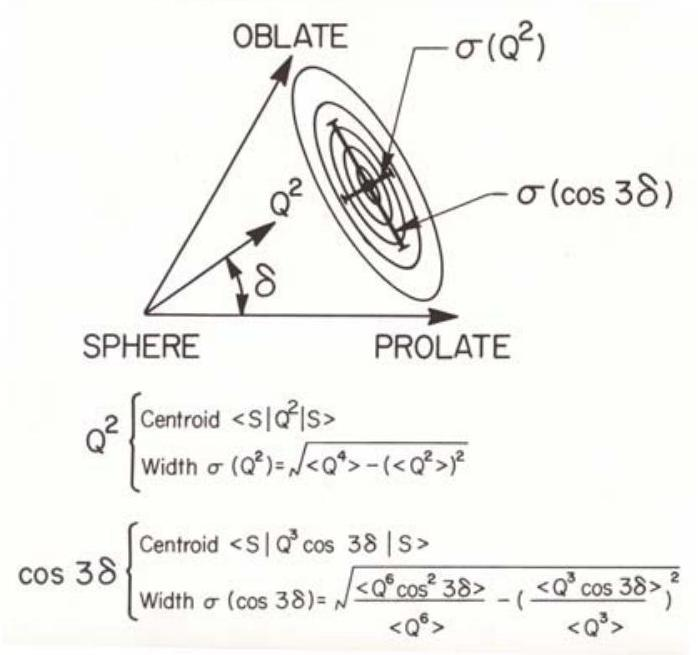
\includegraphics[max width=\textwidth, center]{2025_02_07_204a351db2d7f48b61ebg-222}

Figure 9.1: Distribution plot of the parameters $Q^{2}$ and $\delta$ required to define the E2 properties in the intrinsic frame for a state $S$. All possible E2 moments are defined by the region $Q \geq 0$ and $0 \leq \delta \leq 60^{\circ}$.\\
ground state spin is 0 and the preferable path of excitation involve the $m=0$ magnetic substates for all states. In this case, the $3-\mathrm{j}$ symbol involved in the definition of the coupling parameters $\zeta_{k n}(3.21)$ is:

$$
\left(\begin{array}{ccc}
I & 2 & I \pm 1 \\
0 & 0 & 0
\end{array}\right)=0
$$

since $j_{1}+j_{2}+j_{3}=(2 I+2) \pm 1$ is odd (see e.g.[ROT59]). This means that the lowest significant coupling is the $\Delta m= \pm 1$ coupling being an order of magnitude weaker than the $\Delta m=0$ coupling. Applying the first order perturbation theory $3.36,3.38$ one also finds that due to the antisymmetry of $Q_{2, \pm 1}(\omega)$ this mode of excitation is strongly inhibited. As a result, the $E 2$ matrix elements connecting the even and odd spin states are measured with large errors, unless some additional data, most importantly the branching ratios, are available.

Restricting ourselves to $J=0,2$ and 4 couplings we have from 9.17 and 9.18:


\begin{equation*}
Q^{6} \cos ^{2} 3 \delta(0)=\frac{35}{2} P_{1}^{6}(0)=\frac{35}{2} P_{2}^{6}(0) \tag{9.21}
\end{equation*}


and


\begin{equation*}
Q^{6} \cos ^{2} 3 \delta(J)_{J=2,4}=35\left(P_{1,2}^{6}(4)-\frac{\sqrt{5}}{4} P_{1,2}^{6}(2)\right) \tag{9.22}
\end{equation*}


with


\begin{gather*}
P_{1}^{6}(J)=\frac{5(2 J+1)^{1 / 2}}{2 I_{s}+1} \sum_{r u t v w} M_{s u} M_{u t} M_{t r} M_{r v} M_{v w} M_{w s} \\
\bullet\left\{\begin{array}{ccc}
2 & 2 & J \\
I_{s} & I_{r} & I_{t}
\end{array}\right\}\left\{\begin{array}{ccc}
2 & 2 & 2 \\
I_{s} & I_{t} & I_{u}
\end{array}\right\}\left\{\begin{array}{ccc}
2 & 2 & J \\
I_{s} & I_{r} & I_{w}
\end{array}\right\}\left\{\begin{array}{ccc}
2 & 2 & 2 \\
I_{w} & I_{r} & I_{v}
\end{array}\right\}(-1)^{2 I_{s}+I_{t}+I_{w}} \tag{9.23}
\end{gather*}


and with


\begin{gather*}
P_{2}^{6}(J)=\frac{5(2 J+1)^{1 / 2}}{2 I_{s}+1} \sum_{r u t v w} M_{s u} M_{u t} M_{t r} M_{r v} M_{r w} M_{w s} \\
\bullet\left\{\begin{array}{ccc}
2 & 2 & J \\
I_{s} & I_{r} & I_{t}
\end{array}\right\}\left\{\begin{array}{ccc}
2 & 2 & 2 \\
I_{s} & I_{t} & I_{u}
\end{array}\right\}\left\{\begin{array}{ccc}
2 & 2 & J \\
I_{s} & I_{r} & I_{v}
\end{array}\right\}\left\{\begin{array}{ccc}
2 & 2 & 2 \\
I_{s} & I_{v} & I_{w}
\end{array}\right\}(-1)^{I_{s}+I_{r}+I_{t}+I_{w}} \tag{9.24}
\end{gather*}


Note that 9.21 through 9.24 define three independent estimates of $Q^{6} \cos ^{2} 3 \delta$ - one involving the $J=0$ coupling, identical for both $P_{1}^{6}$ and $P_{2}^{6}$ and two involving the $J=2$ and $J=4$ couplings for $P_{1}^{6}$ and $P_{2}^{6}$, respectively. The value of $Q^{6}(9.19)$ coupled with $Q^{6} \cos ^{2} 3 \delta(J)_{J=2,4}(9.22)$ determines the softness in $\delta$ as being given by the square root of the $\cos 3 \delta$ variance:


\begin{equation*}
v^{2}(\cos 3 \delta)=<\cos ^{2} 3 \delta>-<\cos 3 \delta>^{2} \tag{9.25}
\end{equation*}


The expectation value of $\cos 3 \delta$ can be extracted either from the $Q^{3} \cos 3 \delta$ invariant or three possible values of $Q^{5} \cos 3 \delta$ provided that the expectation values of $Q^{3}$ and $Q^{5}$ are known. These values can be estimated using an interpolation between $Q^{2}, Q^{4}$ and $Q^{6}$. We use:


\begin{align*}
& <Q^{3}>=\left(\frac{1}{2}\left[\left(Q^{2}\right)^{1 / 2}+\left(Q^{4}(0)\right)^{1 / 4}\right]\right)^{3}  \tag{9.26}\\
& <Q^{5}>=\left(\frac{1}{2}\left[\left(Q^{4}\right)^{1 / 4}+\left(Q^{6}(0)\right)^{1 / 6}\right]\right)^{5} \tag{9.27}
\end{align*}


where the $J=0$ coupling for $Q^{4}$ and $Q^{6}$ is used because of the minimum number of the matrix elements involved. This is preferable from a point of view of the completeness of the summation and the error propagation. For the same reason only the expectation value of $\cos 3 \delta$ extracted from $Q^{3} \cos 3 \delta$ is used for the softness in $\delta$.

To summarize, the sum rules derived from the rotational invariants allow measurement of the expectation values of rotational invariants built of $Q$ and $\delta$. Then, as shown in figure 9.1, it is possible to find the statistical distribution of $Q^{2}$ and $\cos 3 \delta$ i.e. the first statistical moments related to the softness in both parameters and the second statistical moment, the skewness (in our case calculated for $Q^{2}$ only). With various $J$-couplings which can be used to evaluate the higher-order invariants, the rotational invariance of the sum rules provide a test of the completeness of the data as well as of the self-consistency of the fitted $E 2$ matrix elements.

\subsection*{9.2 Program SIGMA}
A separate code, SIGMA, has been written to evaluate the quadrupole rotational invariant sum rules. This program has been designed to use the information created by GOSIA (see 7.3), although it can be used separately to calculate the centroids (i.e., the expectation values) of the rotational invariants only, with no error estimation. The following subsection outlines the algorithms used for the computation of the rotational invariants and resulting statistical distribution of $Q$ and $\cos 3 \delta$ and the method employed to estimate the errors of computed values.

\subsection*{9.2.1 Computation of the invariants}
The most efficient way to evaluate the rotational invariants is to use the matrix multiplication formalism having the selection rules for different sum of products superimposed by masking the array of the $E 2$ matrix elements with the appropriate $6-j$ matrices. Let us define (with $s$ being a fixed target state index):


\begin{gather*}
\bar{v}_{L}=\left\{M_{s r}\right\} \text { "left-hand vector" }  \tag{9.28a}\\
\bar{v}_{R}=\left\{M_{r s}\right\} \text { "right-hand vector" }  \tag{9.28b}\\
S_{r v}(J)=\left\{M_{r v}\right\}\left\{\begin{array}{ccc}
2 & 2 & J \\
I_{s} & I_{r} & I_{v}
\end{array}\right\}  \tag{9.28c}\\
S_{r v}^{T}(J)=\left\{M_{v r}\right\}\left\{\begin{array}{ccc}
2 & 2 & J \\
I_{s} & I_{r} & I_{v}
\end{array}\right\}  \tag{9.28d}\\
T_{r v}(J)=\left(\sum_{w} M_{r w} M_{w v}\left\{\begin{array}{ccc}
2 & 2 & J \\
I_{r} & I_{v} & I_{w}
\end{array}\right\}\right)\left\{\begin{array}{ccc}
2 & 2 & J \\
I_{s} & I_{r} & I_{v}
\end{array}\right\} \tag{9.28e}
\end{gather*}



\begin{equation*}
T_{r v}^{\prime}(J)=\sum_{w} M_{r w} M_{w v}(-1)^{I_{w}-I_{s}} \frac{1}{2 I_{r}+1} \delta_{I_{r} I_{v}} \tag{9.28f}
\end{equation*}


The rotational invariants can be expressed in terms of the operators 9.28 as (if the phase needs to be appended, $r$ stands for the row index and $v$ stands for the column index):


\begin{gather*}
Q^{2}=\frac{1}{2 I_{s}+1} \bar{v}_{L} \bullet \bar{v}_{L}  \tag{9.29a}\\
Q^{3} \cos 3 \delta=\mp \frac{\sqrt{35}}{\sqrt{2}} \frac{1}{2 I_{s}+1} \bar{v}_{L} \bullet S(2) \bullet \bar{v}_{R}  \tag{9.29b}\\
Q^{4}(J)=C(J) \bar{v}_{L} \bullet S^{T}(J) \bullet\left[S(J)(-1)^{I_{s}+3 I_{r}}\right] \bullet \bar{v}_{R}  \tag{9.29c}\\
Q^{5} \cos 3 \delta(J)=\mp C(J) \bar{v}_{L} \bullet S^{T}(J) \bullet T(J) \bullet \bar{v}_{L}  \tag{9.29~d}\\
Q^{6}(J)=C(J) \bar{v}_{L} \bullet S^{T}(J) \bullet T^{\prime} \bullet S(J) \bullet \bar{v}_{R}  \tag{9.29e}\\
Q^{6} \cos ^{2} 3 \delta(J)=C(J) \bar{v}_{L} \bullet\left[S(2)(-1)^{I_{s}+I_{w}}\right] \bullet S^{T}(J) \bullet\left[T(J)(-1)^{I_{s}+I_{w}}\right] \bullet \bar{v}_{R}  \tag{9.29f}\\
Q^{6} \cos ^{2} 3 \delta(J)=C(J) \bar{v}_{L} \bullet\left[S(2)(-1)^{I_{s}+I_{r}}\right] \bullet S^{T}(J) \bullet S(J) \bullet\left[S(2)(-1)^{I_{s}+I_{w}}\right] \bullet \bar{v}_{R} \tag{9.29~g}
\end{gather*}


where $C(J)$ are the appropriate constants as defined in the previous subsection and the two formulas for $Q^{6} \cos 3 \delta(J)$ correspond to the coupling schemes 9.17 and 9.18 and $\bar{v}_{L}$, and $\bar{v}_{L}$ are defined by equation 9.28 . The invariants are evaluated according to 9.29 from the right side, so that only the matrix-vector multiplications are performed, without any matrix-matrix multiplications.

\subsection*{9.2.2 Estimation of errors in SIGMA}
The rigorous estimation of the errors of the function of the E2 matrix elements would require the knowledge of all sets of these matrix elements yielding a given value of this functions together with the probability of each such set. Technically it is of course out of question to apply this method to evaluate the errors of the rotational invariants. We are therefore forced to use a crude approximation, which is to assume that the set of the measured matrix elements is contained within an ellipsoidal contour (note that because of the correlation all matrix elements, not only E2, have to be taken into account). This contour is defined by a requested increase of the $S$ statistic (6.65) and its orientation in the space of the matrix elements results from the correlations introduced by a method of measurement. One should be aware that the correlation of the matrix elements introduced by a functional form may be completely different from that resulting from the measurement. As an extreme example it is easily checked that the variance of $Q^{2}$ vanishes if there is only one state of a given spin, whatever values of the matrix elements are used. In this case, the error of the variance is zero, no matter what errors are assigned to the matrix elements.

The error contour, defined by the increase of the $S$ statistic (6.65), is approximated by the quadratic formula:


\begin{equation*}
\Delta S=\delta=\bar{\nabla}_{o} \bullet \Delta \bar{M} \bullet J \bullet \Delta \bar{M} \tag{9.30}
\end{equation*}


where $\bar{\nabla}_{o}$ is the gradient taken at the origin, $\bar{M}_{o}$, while $J$ is the second derivatives matrix:


\begin{equation*}
J_{i k}=\frac{\delta^{2} S}{\delta M_{i} \delta M_{k}} \tag{9.31}
\end{equation*}


and

$$
\Delta \bar{M}=\bar{M}-\bar{M}_{o}
$$

It is easily checked that all points on the contour 9.30 can be parameterized by


\begin{equation*}
\Delta \bar{M}=\bar{M}-\bar{M}_{o}=\frac{2 \delta \bar{e}}{\bar{\nabla}_{o} \bar{e}+\left[\left(\bar{\nabla}_{o} \bar{e}\right)^{2}+2 \delta \bar{e} J \bar{e}\right]^{1 / 2}} \tag{9.32}
\end{equation*}


where $\bar{e}$ is an arbitratry vector. Denoting a given function of matrix elements by $S(\bar{M})$ we have to locate the points $\bar{M}$ on the contour yielding the extremum values of $S(\bar{M})$. Let us consider the function $S(\bar{M})$ which can locally be appoximated by the linear expansion in $\bar{M}$ :


\begin{equation*}
\Delta_{s}(\bar{M})=\nabla_{s} \bullet\left(\bar{M}-\bar{M}_{s}\right) \tag{9.33}
\end{equation*}


where we expand $S(\bar{M})$ in a vicinity of $\bar{M}_{s}$. To find the extrema of 9.33 on the contour 9.30 we have to find the vectors $\bar{e}$ satisfying:


\begin{equation*}
\frac{d}{d \bar{e}}\left(\frac{2 \delta \bullet\left(\bar{\nabla}_{s} \bullet \bar{e}\right)}{\bar{\nabla}_{o} \bar{e}+\left[\left(\bar{\nabla}_{o} \bar{e}\right)^{2}+2 \delta \bar{e} J \bar{e}\right]^{1 / 2}}\right)=0 \tag{9.34}
\end{equation*}


which yields:


\begin{equation*}
\bar{\nabla}_{s}\left(2 \delta-\bar{\nabla}_{o} \bar{e}\right)-\bar{\nabla}_{o}\left(\bar{\nabla}_{s} \bar{e}\right)-\left(\bar{\nabla}_{s} \bar{e}\right) \bullet \bar{J} e=0 \tag{9.35}
\end{equation*}


From 9.35 it is clear that the vector $\bar{e}$ must be a linear combination of $J^{-1} \bar{\nabla}_{s}$ and $J^{-1} \bar{\nabla}_{o}$. Inserting


\begin{equation*}
\bar{e}=\alpha J^{-1} \bar{\nabla}_{s}+\beta J^{-1} \bar{\nabla}_{o} \tag{9.36}
\end{equation*}


into 9.35 we get, using the identity


\begin{equation*}
\bar{\nabla}_{s} J^{-1} \bar{\nabla}_{o}=\bar{\nabla}_{o} J^{-1} \bar{\nabla}_{s} \tag{9.37}
\end{equation*}


resulting from the symmetry of $J$ :


\begin{align*}
& \alpha= \pm\left(\frac{2 \delta+\bar{\nabla}_{o} J^{-1} \bar{\nabla}_{0}}{\bar{\nabla}_{s} J^{-1} \bar{\nabla}_{s}}\right)^{1 / 2}  \tag{9.38}\\
& \beta=-1
\end{align*}


which is valid for any arbitrarily chosen origin $\bar{M}_{o}$. However, in our case we can assume that $\bar{M}_{o}$, the vector of fitted matrix elements, is a close approximation of the minimum, thus $\bar{\nabla}_{o} \approx 0$. Neglecting the terms containing $\bar{\nabla}_{o}$ we finally get:


\begin{equation*}
\bar{M}=\bar{M}_{o} \pm\left(\frac{2 \delta}{\bar{\nabla}_{s} J^{-1} \bar{\nabla}_{s}}\right)^{1 / 2} J^{-1} \bar{\nabla}_{s} \tag{9.39}
\end{equation*}


where a positive sign corresponds to the maximum of 9.33 on the contour 9.30 and a negative sign corresponds to its minimum. This formula gives an exact solution for any linear function of $\bar{M}_{o}$. For non-linear functions 9.39 can be used iteratively following the scheme:


\begin{gather*}
\bar{\nabla}_{s}^{(0)}=\bar{\nabla}_{s}\left(\bar{M}_{o}\right) \Longrightarrow \bar{M}^{(1)} \\
\bar{\nabla}_{s}^{(1)}=\bar{\nabla}_{s}\left(\bar{M}^{(1)}\right) \Longrightarrow \bar{M}^{(2)} \tag{9.40}
\end{gather*}


until the convergence is achieved. This procedure is used in SIGMA to estimate the errors of $Q^{2}, \cos 3 \delta$ and their statistical moments. Because of the fact that the implementation of the rotational-invariant sum rules is only possible for the cases in which virtually all the E2 matrix elements for low lying states are known, implying that the underlying Coulomb excitation problem is well overdetermined, it is reasonable to assume a least-squares statistic increase $\delta=1$. The $J$ matrix is estimated using the gradients computed by GOSIA during the calculation of correlated errors (see 6.6) and stored on a permanent file. Applying the quadratic approximation 9.1 and assuming $\bar{M}_{o}=$ minimum (i.e. $\nabla_{o}=0$ ) one can write:


\begin{equation*}
\bar{\nabla}(\bar{M})=\hat{J}\left(\bar{M}-\bar{M}_{o}\right) \tag{9.41}
\end{equation*}


During the correlated errors calculation GOSIA evaluates the gradients in points $-M$ for which only one matrix element at a time is perturbed from its central value. This means that $\bar{M}-\bar{M}_{o}$ has only one non-zero component, thus 9.41 defines $k$-th column of $J$ if $M_{k}$ has been perturbed. Two estimates of $J_{k i}$ are available using positive and negative values of $\Delta M_{k}$. In addition, $J_{k i}$ can be evaluated using the $i$-th component of the gradient at perturbed $M_{k}$ or using the $k$-th component of the gradient with perturbed $M_{i}$. Since the quadratic approximation 9.1 is not fully adequate, the averaging procedure must be used to cancel the difference between various estimates and to preserve the symmetry of $J$. Furthermore, for the matrix elements $M_{k}$ for which the full error calculation was not performed only the diagonal element $J_{k k}$ is assumed to be non-zero, i.e., the correlation is neglected. The estimate of $\mathrm{J}_{k k}$ in this case results from:


\begin{equation*}
\Delta S=1=\frac{1}{2} J_{k k} \Delta M_{k} \tag{9.42}
\end{equation*}


where $\Delta M_{k}$ is the average diagonal error of $M_{k}$, i.e., the mean value of the negative and positive deviations.\\
The method presented above allows estimation of the errors of the collective parameters and their distributions with reasonable efficiency. However, one must be aware of the scope of the approximations used, which do not allow treating the estimated errors very rigorously, providing only a crude estimate of the determined accuracy of the rotational invariant sum rules.

\subsection*{9.2.3 Sources of systematic errors in SIGMA}
The invariants are model independent and they can be calculated exactly using $E 2$ matrix elements predicted by theoretical models of nuclear structure. Experimentally Coulomb excitation data can only determine a subset of the $E 2$ matrix elements close to the yrast line and thus it is not viable to determine experimentally the complete set of matrix elements required to fully evaluate the rotational invariants. The limitations are discussed in chapter 2.3.3. Sufficient states must be included when evaluating the rotational invariants to ensure complete summing of the appropriate strength for the state of interest[CLI72, CLI86]. Agreement between the identities for different intermediate spin coupling provide one measure to ensure adequate completeness of the summations. Another is to ensure that an appropriate number of all multiphonon steps have been included. For example, the expectation values of $Q^{2}$ and $Q^{3} \cos 3 \delta$ involve summing strength to states having a change in oscillator number of $-1 \leq \Delta n \leq+1$. For invariants involving $Q^{4}$ it is necessary to sum over $-2 \leq \Delta n \leq+2$, while for the $Q^{6}$ invariants it is necessary to sum over $-3 \leq \Delta n \leq+3$. For conventional multiple Coulomb excitation this implies that $E 2$ centroids can be evaluated for excited states up to one less than the highest observed complete oscillator shell, while the ground state is the only state for which a viable measure of the variance is achievable.

\subsection*{9.3 Input instructions}
SIGMA reads in the input file, which must be called SIGMA.INP and in addition three permanent files created by GOSIA, referred to in SIGMA as filename.err [TAPE11], filename.smr [TAPE12] and sixj.tab [TAPE3].

The input file selects the mode of calculation and should be given as:

\section*{IL}
NST\\
filename.smr corresponding to SIGMA TAPE12\\
filename.err corresponding to SIGMA TAPE11\\
sixj.tab corresponding to SIGMA TAPE3\\
I(1)\\
I(2)\\
only if $0<N S T \leq 75$\\
I(NST)

That is, the input file comprises two switches, three filenames, followed by the list of states for which all errors are to be calculated ( $N S T$ records) where:\\
$I L$ may be either 0 or $1 . I L=1$ will cause the printout of the matrix elements (by their indices) involved in the evaluation of 14 invariants calculated for each state. The invariants are numbered from 1 to 14 according to the sequence they appear in the first column of the output table (see the sample output at the end of this chapter). $I L=0$ will cause no compilation of this list.\\
$N S T \quad$ selects the mode of error calculation. Three special values of $N S T: N S T=-1, N S T=0$ or $N S T=99$ require no further input. $N S T=-1$ is used if only the invariants and the resulting statistical moments (given in the second column of the output table) are to be calculated and no error estimation is requested. In this mode SIGMA can be used independently of GOSIA and the information concerning the level scheme and coupling scheme, normally produced by GOSIA, must be provided by the user (see the description of the TAPE files below). $N S T=0$ implies that the error calculation is to be performed only for $Q^{2}$, three values of $v\left(Q^{2}\right)$ and four values of $\cos 3 \delta$ for all states, while $N S T=99$ specifies the errors to be estimated for every statistical moment for all states. The reason for this distinction is that the statistical moments based on the sixth-order invariants are usually not meaningful due to the number of the matrix elements involved and the resulting error propagation. Also, calculation of these invariants is most timeconsuming. Usually, it is practical to calculate all the errors only for the few lowest-lying states. This can be achieved using "mixed" calculation mode, specified by $0<N S T \leq 75$. In this case, NST has the meaning of the number of states for which the "full" calculation is to be done, while for the remaining states the "fast" mode, corresponding to $N S T=0$ will be used. In this mode the list of state indices ( $N S T$ records) must follow.

Note that the errors quoted are the errors of the statistical moments (column 2 of the output table), not of the invariants listed in the first column.

An example is:\\
0\\
0\\
nd.smr\\
nd150.err\\
sixj.tab\\
Permanent Files:\\
TAPE11 This file contains the errors of the matrix elements and is written by GOSIA as TAPE15. It is not required if $N S T=-1$. Use the filename explicitly in the input, e.g. nd150.err

TAPE3 Contains the table of the 6 - j symbols used for the calculation of the invariants. This table can be created by GOSIA with OP,SIXJ (see 7.27). GOSIA writes the table on TAPE14.

TAPE12 This file is written by GOSIA during full error calculation on TAPE3 if the CONT switch SMR, is set. TAPE12 contains the level scheme, the coupling scheme and the set of gradients used to evaluate the $J$ matrix. Use filename explicitly in the input, e.g. nd $150 . \mathrm{smr}$. If SIGMA is to be used independently of GOSIA, (i.e., only if $N S T=-1$ ) a part of this file must be prepared by the user. The format of this portion of TAPE12 should be the following:

NS, NME, NI, NF where\\
$N S=$ number of states\\
$N M E=$ number of matrix elements\\
$N I=$ index of a first E2 matrix element\\
$N F=$ index of a last E2 matrix element

\section*{INDEX (1), SPIN(1), ENERGY(1)}
. Level scheme

\begin{itemize}
  \item NS records
\end{itemize}

INDEX(NS), SPIN(NS), ENERGY(NS)\\
IME(1) $, \mathbf{I N I}(\mathbf{1}), \mathbf{I N F}(\mathbf{1})$ Coupling scheme. IME is the index of matrix element,\\
INI is the index of an initial state\\
INF is the index of a final state.

\begin{itemize}
  \item The GOSIA convention applies to the ordering of the matrix elements (see 5.15).
\end{itemize}

IME(NME), INI(NME), INF(NME) NME records.\\
$\mathbf{I M E}(\mathbf{1}), \mathbf{M E}(\mathbf{1}) \quad$ Values of the matrix elements.\\
NME records

IME(NME), ME(NME)\\
$\mathbf{0}, \mathbf{0} \quad$ Two zeros terminate the input.

\section*{Chapter 10}
\section*{File assignments}
The following chapter provides an overview of the file assignments in GOSIA, SIGMA and SELECT. A permanent or temporary file is referred to as FILEn, where $n$ designates the code-declared file number. An actual name for such a file depends on the operating system of a given computer. To allow the possibility of examining the contents of the permanent files generated by all three codes a free format FORTRAN write ( i.e. $W \operatorname{RITE}(n, *)$ ) is used. The only exception is the internal correction factors File1 (see Section 6.5) which may be frequently updated during the least-squares fit, therefore to speed up the input/output operations the binary format (i.e. WRITE (1) ) has been chosen instead. The short description of the files being used by GOSIA, SIGMA and SELECT is presented in sections 10.1, 10.2 and 10.3 , respectively. The files are classified as input files, i.e. the ones that must be attached to the current job, output files, i.e. the ones that are created by the job and should be saved as permanent files for further use, and internal files, used to transfer the data between some of the modules of GOSIA. The internal files need not be attached to the job or saved after the execution. Both GOSIA and SIGMA require an input file which should be provided by the user in the $R E A D *$ format, (that is, space- or comma-delimited) while no such a file is needed to run SELECT. Section 10.4 provides a series of examples of the typical command sequences together with the lists of the input, output and internal files employed during the execution.

\subsection*{10.1 File assignments in GOSIA}
FILE3 The function of File3 depends on the command being executed. File3 is the input file of the original, uncorrected experimental $\gamma$ yields for OP, CORR ( the output file of the corrected yields will be written on File4 ). Note that if OP,CORR is to be executed the OP,YIEL input entry NTAP (see Section 7.32 ) must equal 3. File3 can also be assigned instead of File4 as an input file of the corrected yields for OP,MINI and OP,ERRO, if the value of $N T A P$ is 3 . To avoid a possible input/output assignment conflict it is, however, recommended to use File 4 when executing OP,ERRO, since File3 is reserved as an output file for the code SIGMA if the CONT switch SMR, is set. In this case File3 is created during a first run of OP,ERRO with $I D F=1$ and $I R E P=1$ (see Section 7.6) and updated if $I D F=1$ and $I R E P=2$.

FILE4 Contains the corrected yields written when OP,CORR is executed. File4 then should be an input file of the experimental yields for both OP,MINI and OP,ERRO with the OP,YIEL entry $N T A P=4$. As discussed above, File3 can also be assigned for this purpose. File4 is also written when OP,POIN is executed with $I F L=1$ (see Section 7.19) to create the simulated "experimental" yields

FILE7 Contains the maps of the q-parameters to be used by the fast Coulomb excitation calculation ( see Section 6.2 ). File7 is written by OP,MAP and read automatically when either the OP,MINI or OP,ERRO command is encountered. This means that the existing permanent file containing the $q$-parameter map should be attached to the minimization or error calculation jobs as File7 unless OP,MAP has been executed before during the same run.\\
FILE8 Contains the absorption coefficients needed to reproduce $\gamma$-ray energy dependence of the detector efficiency. Created if $N P D$ in OP,GDET is negative, which is connected to the use of "raw" spectra as defined by the input to OP,RAW.

FILE9 Contains the parameters needed to approximately reproduce the $\gamma$-energy dependence of the Ge detector solid angle attenuation coefficients $Q_{k}$ ( see Section 6.4 ). File9 is written when OP,GDET is executed and automatically read in when OP,YIEL is encountered, which implies that File9 should be attached to any job involving the calculation of $\gamma$ yields.

FILE11 Contains the internal correction factors ( see Section 6.5 ) created and updated when OP,MINI is executed. File11 is required as an input file if the CONT switch CRF, was selected. CRF, causes GOSIA to read the internal correction factors from File11 instead of calculating them when OP,MINI is encountered. Obviously, File11 is to be saved after a previous run to use the time-saving CRF, switch when resuming the minimization. The internal correction factors are updated (and stored on File11) every time the TEST criterion of the OP,MINI input ( 7.18 ) is fulfilled, thus the internal correction coefficients stored on File11 will correspond to the last set of matrix elements for which the update, defined by TEST, was done. In addition, the internal correction coefficients can be calculated using the CONT switch CCF, for a given set of matrix elements. In this case File11 should be saved and defined as an input file for the subsequent run using the CONT CRF, switch.

FILE12 Contains the set of matrix elements resulting from the last minimization run. File12 is overwritten after completion of each OP,MINI command. The values of the matrix elements stored on File12 can be used instead of those specified in the ME input using the OP,REST command before the selected executable option. An existing permanent file must be assigned to File12 if OP,REST is used.

FILE14 An output file for OP,SIXJ. Contains the table of Wigner's $6-j$ symbols to be used by SIGMA. File14 also serves as an internal file when OP,INTG, OP,INTI, OP,CORR, OP,TROU or OP,MINI with the calculation of the sensitivity maps ( see Section 6.5 ) are executed.\\
FILE15 Contains the current set of errors of the matrix elements calculated by OP,ERRO. File15 is written by OP,ERRO if $I R E P=0$ ( see Section 7.6 ) and read, updated and overwritten if $I R E P=1$. Internal for OP,INTG, OP,CORR and OP,TROU.\\
FILE17 An output file for OP,ERRO, containing the best (i.e. yielding the lowest value of $\chi^{2}$ ) set of matrix elements found during the scan of the $\chi^{2}$ hypersurface (see Section 6.6). Also serves as the output file to write the statistical tensors after Coulomb excitation using the CONT switch TEN, in conjunction with either OP,STAR or OP,POIN (see Section 7.3). The structure of this file, which may be used by external programs to examine the $\gamma$-ray decay following the Coulomb excitation is as follows:

$$
\begin{aligned}
& N \\
& \rho_{00} \\
& \rho_{20}, \rho_{21}, \rho_{22} \\
& \rho_{40}, \rho_{41}, \rho_{42}, \rho_{43}, \rho_{44} \\
& \rho_{60}, \rho_{61}, \rho_{62}, \rho_{63}, \rho_{64}, \rho_{65}, \rho_{66}
\end{aligned}
$$

here $N$ is the level index as defined by the sequence of the input to LEVE. The tensors for the ground state $N=1$ are not stored, thus $2<N<N M A X$ where $N M A X$ is the number of levels included. This sequence is repeated for each experiment according to the sequence of the input to EXPT. Note that because of the symmetry $\rho_{k m}=(-1)^{m} \rho_{k-m}$ only the components with $m>0$ are stored. File17 is also used as an internal file by OP,TROU and OP,INTG.

FILE18 An input file for the program SELECT and for OP,ERRO if the correlation matrix is to be used to reduce the number of correlated matrix elements during a full error calculation ( $I D F=1$ and $I F C=0$ in the OP,ERRO input - see Section 7.6, see also Section 6.6). File18 should be created first using the CONT switch SEL, and the default setting of the print parameter 4 (i.e. -2 ) while executing OP,MINI. File18 should then be attached to the execution of SELECT, the result being written as File10. The latter file can then be attached to the OP,ERRO job as File18. This is internal for OP,TROU.

FILE22 Output file. Unit 22 is used instead of default FORTRAN unit 6 to avoid merging the output with system messages (e.g. underflow warnings) on some systems. During minimization the current value of CHISQ is also output on File6. Dependent on the system, and execution mode, it will appear either on the screen or in log file, which usually can be viewed during execution. This helps to decide whether or not interrupt the job if no progress is made.

FILE23 Lists the Doppler-shifted $\gamma$-ray energies and detector efficiencies when OP,POIN is executed in conjunction with OP,RAW.

\subsection*{10.2 File assignments in SIGMA}
SIGMA requires three input File files - File11, File12 and File3. All three files are written by GOSIA. However, if no error estimation of the invariants is desired, it is not necessary to attach File11, and only a part of File12 is needed - see Section 9.2.2 for details. SIGMA produces no output files other than the printer output. The input file assignments are the following:

FILE11 Contains the errors of the matrix elements, equivalent to the GOSIA output file File15.

FILE12 Equivalent to the GOSIA output file File3 written during the calculation of the full errors (OP,ERRO with $I D F=1$ and the CONT switch SMR).

FILE3 The table of the $6-j$ symbols created by GOSIA as File14 using OP,SIXJ.

FILE23 The printer output file.

\subsection*{10.3 File assignments in SELECT}
SELECT requires one input File file, File18, written by GOSIA and no user-given input. The file assignments are as follows:

FILE6 The printer output file.

FILE10 Output file, containing the "correlation matrix", i.e. the square matrix, indexed by the indices of the matrix elements and having the elements either equal to 0 ( no correlation detected) or to 1 ( correlation detected ). This matrix should be attached to the OP,ERRO job when calculating the correlated errors as File18.

FILE18 Input file, containing the information written by GOSIA also on File18 during the execution of OP,MINI with the CONT switch SEL, set and the print parameter 4 equal to -2 .

\subsection*{10.4 Examples of input files and file assignments for typical jobs}
This section provides some examples of the file assignments necessary to run typical jobs. The schematic examples of the input streams, ordered according to the usual sequence of the jobs run to analyze a given case, are followed by the list of the input and output files. Details of each section omitted for brevity are marked by dots. The user-given input file and the printer output file (File22 in GOSIA, File23 in SIGMA, File6 in SELECT) are not listed. OP,TITL is always optional and can be skipped. It is also assumed that for all the jobs involving minimization or error calculation (i.e. starting from 10.3.4.) the corrected experimental yields reside on file File4.

\subsection*{10.4.1 Coulomb excitation amplitudes}
\begin{verbatim}
OP,TITL
OP,GOSI
LEVE
.
ME
EXPT
    .
    CONT
    .
END,
OP,STAR
OP,EXIT
Input: None
Output: None
\end{verbatim}

Comments: This job can be run with both OP,GOSI and OP,COUL. Adding the CONT switch TEN, will cause creation of the output file File17 ( the statistical tensor file ).

\subsection*{10.4.2 Creation of the Ge detectors file}
\section*{OP,TITL}
OP,GDET

OP,EXIT\\
Input: None\\
Output: File9 (File8)\\
Comments: The file File9 is needed as input for all jobs involving the calculation of the $\gamma$ yields. It is not necessary to select OP,COUL or OP,GOSI to run OP,GDET. File8 is necessary only if OP,RAW is to be used.

\section*{Calculation of the $\gamma$-ray yields by point approximation}
OP,TITL\\
OP,GOSI\\
LEVE\\
.\\
ME\\
.\\
EXPT

CONT\\
(TEN,)\\
.\\
END,\\
OP,YIEL

OP,POIN\\
IFL,YLIM\\
OP,EXIT

Input: File9\\
Output: File4 if IFL=1, File17 if the CONT switch TEN, is selected.\\
Comments: This job can be run with either OP,COUL or OP,GOSI. The OP,YIEL\\
entry NTAP must equal 0 .

\subsection*{10.4.3 Calculation of the integrated $\gamma$-ray yields and generation of a "corrected" experiments yields file}
\begin{verbatim}
OP,TITL
OP,GOSI
LEVE
.
ME
.
EXPT
CONT
END,
OP,YIEL
OP,INTG
OP,CORR
OP,EXIT
Input: File3,File9
Output: File4
\end{verbatim}

Comments: The OP,YIEL entry NTAP must equal 3 (i.e. the original experimental yields must reside on File3). OP,INTG can be executed without a subsequent OP,CORR, in this case NTAP must equal 0 , File3 need not be attached and no output file is written.

\subsection*{10.4.4 Calculation of the q parameter map}
\begin{verbatim}
OP,TITL
OP,GOSI
LEVE
.
ME
EXPT
CONT
\end{verbatim}

END,\\
OP,YIEL

OP,MAP\\
OP,EXIT

Input: File4,File9\\
Output: File7\\
Comments: The maps of the q-parameters can be calculated without entering the decay-related information contained in the input to OP,YIEL. However, these maps are only needed for the fitting of the matrix elements, so the deexcitation data are usually already included in the input.

\subsection*{10.4.5 Minimization run - initial stage}
OP,TITL\\
OP,GOSI\\
LEVE\\
.\\
ME\\
.\\
EXPT\\
.

CONT\\
FMI,\\
PRT,\\
4,0\\
.\\
0,0\\
.\\
END,\\
OP,YIEL

OP,MINI

OP,EXIT

Input: File4,File7,File9\\
Output: File11,File12

Comments: In this example it is assumed that the q-parameter map (File7) has been generated during a previous run. OP,MAP can be executed before OP,MINI in the same run in which case File7 should not be attached as an input file, but will appear as an output file instead. The PRT, entry 4,0 switches off the time-consuming calculation of the sensitivity map and is recommended during the initial stage of the minimization. To further speed up the fitting procedure one can also use the CONT switch FMI, if the printout of the comparison of the fitted and experimental data is not crucial. Usually one needs this table only periodically, so it is recommended to generate it separately when needed, by setting a high value of CHILIM in MINI command to inhibit actual minimization. This procedure is also more reliable, since it refreshes the normalization constants.

\subsection*{10.4.6 Minimization - final stage}
\begin{verbatim}
OP,TITL
\end{verbatim}

OP,GOSI\\
LEVE\\
ME\\
EXPT\\
CONT\\
CRF,\\
SEL,\\
.\\
END,\\
OP,YIEL\\
OP,REST\\
OP,MINI\\
OP,EXIT

Input: File11,File12,File4,File7,File9\\
Output: File11,File12,File18

Comments: The CONT switch SEL, in conjunction with the default setting of the print parameter 4 ( i.e. -2 ) causes the generation of an output file File18, containing the information used by the code SELECT to create the correlation matrix, subsequently used during the error calculation. OP,REST causes GOSIA to use the values of the matrix elements stored on File12 instead of those given in the ME input. The internal correction factors file File11 may be updated if the TEST criterion is fulfilled.

\subsection*{10.4.7 SELECT - correlation matrix generation}
No user-given input is required to run SELECT. The only files needed are:\\
Input: File18, created by GOSIA as File18, as described above.\\
Output: File10, containing the correlation matrix.

\subsection*{10.4.8 Diagonal error calculation}
OP,TITL\\
OP,GOSI\\
LEVE\\
.

ME

EXPT\\
.\\
CONT\\
CRF,\\
.\\
END,\\
OP,YIEL

OP,REST

OP,ERRO\\
0,MS,MEND, 0,0, RMAX\\
OP,EXIT\\
Input: File11,File12,File4,File7,File9\\
Output: File15\\
Comments: This example assumes the first diagonal error calculation, so IREP $=0$ and File15 is not attached as an input file. To resume the diagonal error calculation the input to OP,ERRO should be modified as follows:

OP,ERRO\\
0,MS,MEND, 1,0, RMAX\\
and the file File15 should be attached as an input file. File15 will be updated and overwritten. It is also assumed that the internal correction factors (File11) and the current set of matrix elements (File12 ) are those generated by the last OP,MINI run.

\subsection*{10.4.9 Calculation of the correlated errors}
\begin{verbatim}
OP,TITL
OP,GOSI
LEVE
    .
    ME
EXPT
CONT
CRF,
SMR,
END,
OP,YIEL
OP,REST
OP,ERRO
1,MS,MEND,1,0,RMAX
OP,EXIT
\end{verbatim}

Input: File11,File12,File4,File7,File9,File15,File18\\
Output: File3,File15,File17 if sets of matrix elements yielding better values of $\chi^{2}$ were found during the run.

Comments: The above example assumes that the file for the sum-rules code SIGMA ( File3 ) is to be created and that the correlation matrix ( File18) is to be used during the error calculation. If more than one run is necessary to perform the full error calculation one should modify the input to OP,ERRO as follows to resume the job:

OP,ERRO\\
1,MS,MEND, 2,0,RMAX\\
and attach File3 as an input file. File3 will be updated and overwritten by the current job.

\subsection*{10.4.10 6-j symbols table}
OP,TITL\\
OP,SIXJ\\
OP,EXIT\\
Input: None\\
Output: File14\\
Comments: OP,SIXJ can be inserted anywhere in the command sequence, in which case the input files required by the preceding options must be attached.

\section*{Chapter 11}
\section*{Simultaneous Coulomb excitation: GOSIA2 }
GOSIA2, developed by Tomasz Czosnyka, is a special version of GOSIA that is intended to handle either target or projectile excitation are observed in a single experiment. This avoids introducing free parameters (normalization constants) which is important when only a very limited number of experimental data result from the experiment, such as using radioactive beams and when the Rutherford scattering cross section is not measured simultaneously to provide a normalization. As an extreme case one can imagine the situation in which only the lowest transition is observed, then there are at least two parameters; the matrix element and the normalization constant. Simultaneous inclusion of the transitions originating from the second partner and possibly known spectroscopic data makes it possible to achieve a unique solution. The problem of arbitrary normalization constants does not exist in case of multiple COULEX, where both the number of fitted matrix elements and the number of experimental data is large enough to neglect the impact of introducing a few more parameters fitted by the regular code GOSIA.

GOSIA2 requires two parallel inputs describing both collision partners. It was chosen to maintain separate inputs rather than merging them to form a single one to preserve maximum compatibility with the regular GOSIA input. One can switch to GOSIA by deleting only three input records. Using GOSIA relieves some restriction imposed by GOSIA2 when the use of GOSIA is justified. At the stage of fitting matrix elements GOSIA2 will switch between the two inputs. This results in the necessity of observing some conventions imposed by the GOSIA2 logic. The most important one is that experiments in both inputs and experimental data sets should be ordered parallel, i.e. experiment $\# n$ in the first input should be the same as experiment $\# n$ in the second. Then the common normalization constant will be found by the code. All geometric factors are included in the calculations without arbitrary renormalization. In the best case the experiments should be coupled together, like in GOSIA (although this is not required). In this situation there is only one constant remaining, reflecting "flux" or the total number of particles irradiating the target. An example of such organization of inputs is given below.

GOSIA2, as with GOSIA, has two main modes. The first is the Coulomb Excitation calculation which is designated by the OP,COUL section. The other is the experimental fit which is designated by OP,GOSI. Both of these options are input to GOSIA2 in the same manner as one would with GOSIA. The process for running the two functions is different.

To run the OP,COUL calculation the input files must be created using the guidelines described in the manual, the projectile and target input files are referred to as input1.inp and input2.inp respectively. It is important to note that each file requires a separate execution when calculating the gamma-ray yields. To execute each file type the following:\\
gosia $2<$ input1.inp\\
The output will then be written according to the designated output file in OP,FILE. The same input form is used to execute the target file for target excitation, making sure to replace input1.inp with input2.inp.

To run the OP,GOSI portion of GOSIA2 the process is slightly more complicated. As with GOSIA each file must be run three separate times for the fit to be executed, once with OP, CORR, once with OP,MAP and once with OP,MINI. Once the inputs are prepared the execution is done as follows. First run each file, projectile and target, with OP,CORR using,\\
gosia $2<$ input1.inp\\
gosia $2<$ input2.inp\\
A file should be written with the corrected yields for both the projectile and target. Where the files are located will depend on whether or not there was a specific designation for the output in OP,FILE. Next each file should be run with OP,MAP. The execution is the same as before. Finally the projectile file should be run with OP,MINI. Again, the execution is the same as before.

GOSIA2 has been upgraded in parallel with GOSIA to maintain uniformity of both codes.\\
An example of inputs is intended to reflect a typical MINIBALL experiment. Note that actual numbers are not real (e.g. level schemes are not, so krypton is not really krypton, carbon is not really carbon etc. The aim of the inputs is to demonstrate their structure. The inputs illustrate the situation of "Kr" beam scattered by a "C" target. Particle detectors form a ring in such a way that only "C" particles can be detected, "Kr" going through a central hole as discussed in 6.5.2. The GOSIA2 commands are in bold, the non-bold comments should not be entered into the input file.

\subsection*{11.1 Input instructions}
Important - to avoid confusion execute one executable option at a time. The only exceptions are the sequences OP,REST+OP,MINI and OP,INTG+OP,CORR

1 Input identifier - associates this input with a filename (see below). Remove for GOSIA compatibility\\
OP, FILE Option to name the files which will be used. Not all of them is needed in every step, but the list below is complete, thus it is convenient to keep it full\\
$\mathbf{2 2}, \mathbf{3}, \mathbf{1} 22$ is GOSIA(2) unit number (TAPE in the manual), 3 defines status=unknown, while $1=o l d$, $2=$ new. Third entry means „formatted".\\
kr88.out Output filename.\\
$\mathbf{2 5}, \mathbf{3}, \mathbf{1}$ Unit 25 corresponds to input identifier 1. Remove for GOSIA compatibility. Start GOSIA2 with GOSIA $2<\mathrm{kr} 88 . \mathrm{inp}$, then the code will switch between inputs itself.\\
kr88.inp The name of this input.\\
$\mathbf{2 6}, \mathbf{3}, \mathbf{1}$ Same as above for C12 input.\\
c12.inp\\
$14,3,1$\\
dum. 14 Usually internal, as defined in GOSIA manual.\\
$17,3,1$\\
dum. 17 As above.\\
$\mathbf{1 5}, \mathbf{3}, \mathbf{1}$ Used for error estimation, otherwise internal.\\
dum. 15 As above.\\
\href{http://kr88.me}{kr88.me} Current set of matrix elements in Kr. Written by OP,MINI, read by OP,REST\\
32, 3, 1\\
\href{http://c12.me}{c12.me} As above for C.

\section*{$9,3,1$}
det.inp Gamma detectors file created by OP,GDET. Requested by options involving calculation of gamma yields. Assumed to be the same for Kr and C (detector setup is identical).

\section*{11, 3, 2}
crf.dat Internal, unformatted to save space. Updated by GOSIA2 for Kr and C .

\section*{$3,3,1$}
\href{http://kr88.org}{kr88.org} Here „uncorrected", yields reside. See below.

\section*{27, 3, 1}
c12.map A map of parameters for fast approximation for C. Required for OP,MINI and OP,ERRO. Created by OP,MAP.\\
$7,3,1$\\
kr88.map As above for Kr.

\section*{$4,3,1$}
kr88.cor Kr corrected yields file. See OP,CORR.\\
18, 3, 1\\
dum. 18 Internal.\\
23, 3, 1\\
kr88.raw Used by OP,RAW (OP,RAW is optional).\\
33, 3, 1\\
kr88.smr Sum-rules file for quadrupole sum-rules code SIGMA. Created by OP,ERRO if CONT switch SMR, was set.

\section*{13, 3, 1}
cnor.dat Normalization constants file used by OP,MINI and OP,ERRO.\\
$\mathbf{0}, \mathbf{0}, \mathbf{0} \quad$ End of file definitions\\
OP, TITL\\
Projectile excitation of Kr88 Optional, causes the user-given title to be reprinted in the output\\
Here the definition of the problem starts. The only executable option which can be run at this point is OP,SIXJ if one wants to create a Wigner 6-j file, needed by SIGMA code. It will be written on unit 14 and GOSIA(2) will stop. Resulting file 14 should be renamed and kept for further use.

OP, GOSI Tells the code that fitting of the matrix elements is foreseen. Alternatively OP,COUL can be used if only the excitation part is of interest. OP,COUL simplifies the input of matrix elements. OP,GOSI requires the following suboptions:

LEVE Level scheme of the nucleus.\\
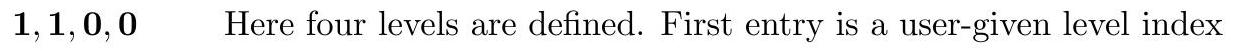
\includegraphics[max width=\textwidth, center]{2025_02_07_204a351db2d7f48b61ebg-241}\\
$\mathbf{2}, \mathbf{1}, \mathbf{2}, \mathbf{7}$ that the code will refer to in the output. Ground state must be given index $=1$,\\
$\mathbf{3}, \mathbf{1}, \mathbf{4}, \mathbf{1 . 5}$ the rest is arbitrary. Here there are four levels defined. Second entry

4, 1, 2, 1.2 is parity +1 or -1 . The third one is spin, while the fourth is level energy in MeV.\\
$\mathbf{0}, \mathbf{0}, \mathbf{0}, \mathbf{0} \quad$ Four zeros ends input\\
ME Definition of starting matrix elements.\\
$\mathbf{2}, \mathbf{0}, \mathbf{0}, \mathbf{0}, \mathbf{0} \quad$ Multipolarity; 2 means $E 2$.\\
$\mathbf{1}, \mathbf{2}, \mathbf{8}, . \mathbf{0 1}, \mathbf{2}$ Matrix elements-initial state index (as defined by LEVE), final state index, value (eb),\\
$\mathbf{1}, \mathbf{4}, . \mathbf{1}, \mathbf{- 1}, \mathbf{1}$ lower and upper limits the matrix element is allowed to change during fitting\\
$\mathbf{2}, \mathbf{2},-\mathbf{5},-\mathbf{1}, \mathbf{1}$ and error estimation. Note that ME's appear in odometric order by indices,\\
$\mathbf{2}, \mathbf{3}, \mathbf{1} ., . \mathbf{0 1}, \mathbf{2}$ i.e. final increases first, initial second\\
$2,4, .2,-1,1$\\
$3,3,-.7,-2,2$\\
$3,4, .2,-1,1$\\
$4,4, .2,-1,1$\\
$\mathbf{7}, \mathbf{0}, \mathbf{0}, \mathbf{0}, \mathbf{0} \quad E 2$ exhausted, now $M 1$. First entry $=6+M$ multipolarity ( 1 and 2 allowed).

\section*{$2,4, .5,-2,2$}
$\mathbf{0}, \mathbf{0}, \mathbf{0}, \mathbf{0}, \mathbf{0} \quad$ First entry $=0$ means that ME setup is complete\\
EXPT Definition of experiments at mean values of scattering angle and energy\\
$\mathbf{2 , 3 6}, \mathbf{8 8} \quad$ Two experiments, $Z, A$ of investigated nucleus\\
$-\mathbf{6}, \mathbf{1 2}, \mathbf{1 9 4},-\mathbf{4}, \mathbf{3}, \mathbf{1}, \mathbf{0}, \mathbf{0}, \mathbf{3 6 0}, \mathbf{0}, \mathbf{1} \quad$ First experiment $-Z$ of uninvestigated nucleus (minus appended means projectile excitation, i.e. Kr is projectile). A of uninvestigated nucleus. Bombarding energy (MeV) Projectile scattering angle(deg). Appended minus sign tells that actually the target was detected. The number of magnetic substates from the starting $m$ of the ground state to be used in the calculation using the full COULEX formalism, number of magnetic substates to be included in the fast approximation (0 or 1 ). Particle detector axial symmetry flag, 0 means axial symmetry, $\phi$ range of particle detector, redundant for axial symmetry. Kinematics flag -0 means larger CMS solution if projectile is heavier than target, 1 otherwise. Coupling of experiment normalizations, for the first experiment it is coupled to itself.\\
$-6,12,194,-6.4,3,1,0,0,360,0,1 \quad$ As above, differs by scattering angle. Last entry specifies common normalization with experiment 1 (see OP,YIEL).

CONT As in GOSIA. Some print defaults changed, so to custom-make your input use PRT,\\
END, END, concludes CONT, End must be followed by a blank line. Empty record is the end of OP,GOSI input.

Before OP,YIEL, OP,GDET must be executed only once to create a file (Unit9). Remove the OP,GDET sequence after executing OP,GDET.

Assuming that all gamma detectors are physically identical one inserts:

\section*{OP, GDET}
1 One physical detector (geometry)\\
$.0001, \mathbf{3 . 5}, \mathbf{1 0}, 10$ Radius of inactive core (historical), radius of the crystal, length of the crystal, distance from target to the detector face -all in cm .\\
$\mathbf{0}, \mathbf{0}, \mathbf{0}, \mathbf{0}, \mathbf{0}, \mathbf{0}, \mathbf{0}$ Thicknesses of $\mathrm{Al}, \mathrm{C}, \mathrm{Fe}, \mathrm{Cu}, \mathrm{Ag} / \mathrm{Cd} / \mathrm{sn}, \mathrm{Ta}$ and Pb absorbers in front of the detector. Here no absorbers are specified.

OP, EXIT End of execution, the remainder of the input ignored.

Note that the Coulex amplitudes and level populations can be calculated using:

\section*{OP,STAR \\
 OP,EXIT}
The gamma-yields related portion of the input starts:

\section*{OP, YIEL}
0 Correction for in-flight decay changing the geometry of gamma detectors. 0 means no correction, 1 tells the code to apply it.

5,2 Number of energy meshpoints and multipolarities to define internal conversion coefficients for Kr.\\
$.05, .1, .4, .8,1 . \quad$ Energy meshpoints (MeV)\\
2 E2\\
$\mathbf{1}, \mathbf{1}, \mathbf{1}, \mathbf{1}, \mathbf{1}$ ICC's for E2 (here of course not real\\
7 M1\\
1, 1, 1, 1, $\mathbf{1}$ As above\\
2, - $\mathbf{2}$ Number of gamma detectors for each experiment. Here two detectors are defined. Minus sign appended to the second entry signifies that gamma detector setup is identical to this defined for previous experiment (common situation)\\
$\mathbf{1 , 1}$ Definition of the "physical" detectors as they appear in OP,GDET. There we assumed that all detectors are physically identical and we defined only one, so for experiment 1 both detectors are the same, as well as for experiment 2.\\
$\mathbf{5}, \mathbf{9 0} \quad \theta$ angles of the gamma detectors\\
$\mathbf{0}, \mathbf{0} \quad \phi$ angles of the gamma detectors\\
In the case of a non-identical detector setup the above sequence should be defined for each experiment.

2, $\mathbf{1}$ Normalization transition (level \#2 to level \#1). Used only for printout and simulation of experimental yields by OP,POIN.

2 Number of data sets, usually equal to the number of detectors unless clusters were formed by OP,RAW. Given for experiment 1, experiment 2 assumed to have identical setup.

1000, 1000 Upper limits of the transition intensities relative to the normalization transition for both detectors. If exceeded for the transitions not given as observed the contribution to least-squares function is added. Here this feature is practically switched off.

1,1 Relative normalization constants of gamma detectors. The values should be the same for efficiencycorrected spectra or if OP,RAW is used.

4 Defines the file experimental „corrected" yields reside on. See also OP,POIN.\\
$\mathbf{0}, \mathbf{0}$ Numbers and weigths of available spectroscopic data - branching ratios,\\
$\mathbf{0}, \mathbf{0}$ lifetimes, mixing ratios and known matrix elements.\\
$\mathbf{0}, \mathbf{0}$ First 0 means no data available, otherwise the input is like in GOSIA.\\
0, 0

\section*{OP, POIN}
$\mathbf{0 , 0}$ or 1,limit, Optional, 0,0 - calculation of "point" yields just for printout. 1,limit causes additionally creation of the simulated experimental yields file containing all transitions of intensities exceeding the value of limit with respect to the normalization transition specified in OP,YIEL. This file will be written on unit 4. When executing OP,POIN the unit selector in OP,YIEL (in this example $=4$ should be set to 0 .)

OP,INTG Performs integration over target thickness and particle detectors ranges\\
$\mathbf{3}, \mathbf{5}, \mathbf{1 9 0}, \mathbf{1 9 4}, \mathbf{1 7 . 8}, \mathbf{2 8} \quad$ Number of energy and theta meshpoints, energy range, theta range of detected particle, in this case target.

190, 192, 194 Energy meshpoints\\
$\mathbf{- 3}, \mathbf{- 3 . 5},-\mathbf{4} .,-\mathbf{4 . 5},-\mathbf{5} . \quad$ Projectile scattering angle meshpoints (appended minus sign when target was actually detected)\\
$\mathbf{3}, \mathbf{5}, \mathbf{1 9 0}, \mathbf{1 9 4}, \mathbf{2 8}, \mathbf{3 2 . 8} \quad$ Number of energy and theta meshpoints, etc. for experiment $2 .$.\\
$190,192,194$\\
-5., -5.7, -6.4, -7.1, -7.71 As above, for experiment 2.\\
3 Number of meshpoints to define $\mathrm{dE} / \mathrm{dx}$\\
190, 192, 194 Meshpoints\\
$10,10,10 \quad \mathrm{dE} / \mathrm{dx}$ values\\
20, 20 Number of subdivisions for numerical integration\\
0 Use the same $\mathrm{dE} / \mathrm{dx}$ table for experiment 2\\
20, $\mathbf{2 0}$ Number of subdivisions for experiment 2.\\
In the present case input to OP,INTG is very simple - we defined axially symmetric ring detectors, so it is not necessary to define theta-phi dependence to reproduce arbitrary shape. Also the geometry is identical for both experiments. This corresponds to usual MINIBALL situation. OP,INTG offers the full description of an experiment, not only-as OP,POIN does-limited to mean values of bombarding energy and scattering angle. Input to OP,INTG is identical to that of GOSIA.

OP, CORR Converts the experimental yields (unit 3) to the values corresponding to "point yields" (unit 4). Corrected yields thus replace „original" yields and are subsequently used in the fitting procedure. Should immediately follow OP,INTG

OP, REST Overwrites the set of matrix elements defined by ME. Should be used when re-running the code.

1,.5 Matrix element $\# 1$ set to .5 by hand. Of course remove this when running the fit again, otherwise once again the value will be reset.\\
$\mathbf{0 , 0}$ Ends the input.\\
A sequence

\section*{OP, REST}
0,0\\
means read the matrix elements as stored with no hand-made changes

\section*{OP, MINI}
$\mathbf{2 1 0 0}, \mathbf{5}, .0001, . \mathbf{0 0 0 1}, \mathbf{1 . 0 1}, \mathbf{0}, \mathbf{0}, \mathbf{1}, \mathbf{0}, \mathbf{0}$ Fitting parameters as in GOSIA, but the way GOSIA2 treats fitting is different. GOSIA2, along with fitting the matrix elements fits normalization constants in such a way that the constants are the same for corresponding datasets from both projectile and target excitation. The parameters given here are recommended ones. Before OP,MINI is executed OP,MAP must be executed (only once for each case (projectile or target excitation).

OP , ERRO Estimation of errors of fitted matrix elements and optionally creation of SIGMA input file. Executed separately for both target and projectile exactly like in GOSIA.

Parallel input for target - very similar to that of projectile. Below there is a list of options just pointing out what are the differences (easy to guess):

2 -input must be labelled 2\\
OP,FILE —— change kr88 to c12 where appropriate\\
22,3,1\\
c12.out\\
25,3,1\\
kr88.inp\\
26,3,1\\
c12.inp\\
14,3,1\\
dum. 14\\
$17,3,1$\\
dum. 17\\
$15,3,1$\\
dum. 15\\
12,3,1\\
\href{http://kr88.me}{kr88.me}\\
32,3,1\\
\href{http://c12.me}{c12.me}\\
9,3,1\\
det.inp\\
11,3,2\\
crf.dat\\
$3,3,1$\\
\href{http://c12.org}{c12.org}\\
27,3,1\\
c12.map\\
4,3,1\\
c12.cor\\
7,3,1\\
kr88.map\\
18,3,1\\
dum. 18\\
33,3,1\\
c12.smr\\
13,3,1\\
cnor.dat\\
$23,3,1$

\begin{verbatim}
c12.raw
0,0,0
OP,TITL
Target excited — or any other title
OP,GOSI
LEVE level scheme of c12 instead of kr88
1,1,0,0
2,1,2,.8
3,1,4,2.
4,1,2,1.
0,0,0,0
ME —-c12 matrix elements
2,0,0,0,0
1,2,.8,.01,2
1,4,.1,-1,1
2,2,-.5,-1,1
2,3,1...01,2
2,4,.2,-1,1
3,3,-.8,-2,2
3,4,.2,-1,1
4,4,.2,-1,1
7,0,0,0,0
2,4,.5,-2,2
0,0,0,0,0
EXPT —investigated and uninvestigated nuclei interchanged, target excitation
2,6,12
36,88,194,-4,3,1,0,0,360,0,1
36,88,194,-6.4,3,1,0,0,360,0,1
CONT
END,
OP,YIEL _internal conversion coefficients for c12, otherwise the same, until...
0
5,2
.05,.1,.4,.8,3.
2
.5,.5,.5,.5,.5
7
.5,.5,.5,.5,.5
2,-2
1,1
5,90
0,0
2,1
2
1000,1000
1,1
4
0,0
1,1 spectroscopic data, here lifetime of the first excited state known
2,1.024,.02
0,0
0,0
Remaining options as in Kr input
\end{verbatim}

\section*{Chapter 12}
\section*{Coulomb excitation of isomeric states: PAWEL}
The code PAWEL is a modification of GOSIA designed by Tomasz Czosnka to handle those special cases where a fraction of the Coulomb excited nuclei have an excited isomeric state as an initial state rather than the ground state. The only change to the standard GOSIA input is the addition of a first record after EXPT containing one number that is the abundance of the nuclei in the isomer state expressed in \%. By convention the isomeric state must be level $\# 2$ in the LEVE setup. Otherwise there are no other changes to the standard GOSIA input.

The operation of PAWEL is similar to GOSIA. except that up to the stage of calculating statistical tensors PAWEL performs two passes. For the first pass the initial conditions are set in such a way that at minus infinity the excitation amplitude is set to unity for state $\# 1$ and to zero for all other states. For the second pass state $\# 1$ is replaced by state $\# 2$. Then both solutions are merged according to the user-given proportion between the ground and isomeric states. The deexcitation part remains unchanged after merging the statistical tensors, so there is only one calculation. The same applies for the fast approximation.

\section*{Chapter 13}
\section*{Minimization by simulated annealing, Option ANNL }
The problem of minimizing an arbitrary function can be approached computationally using a wide variety if techniques; some approaches are better suited to certain problems than others. A common feature of most of these techniques is that steps are taken iteratively in the variable space which reduce the "cost" function (whatever function is being minimized). For a one-dimensional minimization problem with cost function $\mathrm{C}(x)$, a step $\Delta x$ is chosen so that $\mathrm{C}(x+\Delta x)<\mathrm{C}(x)$ and repeated steps are taken in $x$ until the value of $x$ for which $\mathrm{C}(x)$ is a minimum is found. This approach will be referred to here as "strict minimization", since the cost function is never allowed to increase as the minimization procedure is executed. This is a logical and efficient approach, but certain problems will not be solved properly by this method. Specifically, if the function being minimized has several local minima, only one of which is the true global minimum of the function, strict minimization will only converge to the global minimum if the starting point is chosen somewhere in the "well" of the global minimum. Any algorithm which only takes steps "downhill" runs the risk of not converging to the global minimum, unless it is started at a point sufficiently close to this global minimum. For example, if a strict minimization procedure is used to find the minimum of the function shown in Figure 13.1 and the starting point is chosen in region II, the procedure will converge to a value of $x \approx+1.4(C(x) \approx 8.8)$, rather than the global minimum value at $x \approx-2.0(C(x) \approx 2.2)$. The general location of the global minimum is often known in physics-related problems from a consideration of the physical properties of the system in question. In large Coulomb-excitation problems, however, the fit quality may be sufficiently dependent on certain unknown quantities such as the sign of a static E2 matrix element that an alternative to strict minimization should be considered. The method of Simulated Annealing (SA) is an attempt to overcome this shortcoming of standard minimization techniques by allowing some steps uphill, in a controlled fashion.

\subsection*{13.1 The Development of Simulated Annealing}
In 1953, Metropolis et al. showed that it is possible to reproduce the thermodynamic properties of a system of particles by what amounts to a Monte-Carlo integration over configuration space [Me53]. The method proposed by Metropolis involves beginning with these particles (or molecules) in a lattice, and choosing new configurations with a probability $e^{-E / k T}$ (Where $E$ is the energy of the configuration, $T$ is the temperature and $k$ is the Boltzmann constant). These configurations are used in computing statistical properties of the system by averaging the value of such properties in the space of these configurations, and weighting the configurations evenly. In order to accomplish this, new configurations are generated from an initial configuration by considering motions of each particle, and accepting steps for which $\Delta E<0$ with probability one, and accepting steps for which $\Delta E>0$ with probability $\mathrm{e}^{-E / k T}$. This method accurately reproduced the\\
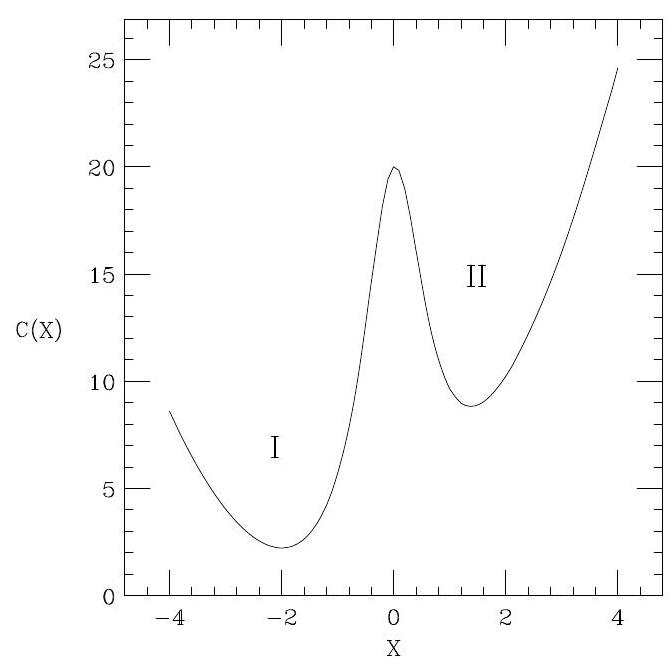
\includegraphics[max width=\textwidth, center]{2025_02_07_204a351db2d7f48b61ebg-250}

Figure 13.1: An example of a function which can cause difficulties with strict minimization procedures. A procedure using a starting value of $x$ in region " II " $(x>0)$ will not converge to the global minimum at $x \approx-2.0$.\\
equation of state for a two-dimensional system (the ratio $P A / n k T$ as a function of $\bar{n}$, the average density of particles at the surface of one particle).

The extension of this method to minimization procedures is obvious: since the Boltzmann-like energy weighting reproduces physical thermodynamic properties, it is theoretically possible, by slowly lowering the temperature of the simulated numeric system, to find the global minimum of the system, analogously to the process of annealing of crystals. In the following discussion, the method of Simulated Annealing will be described for problems of one dependent variable only. The adaptation of this method to multi-variable minimization problems will be discussed later.

The Simulated Annealing method in its most general terms is described as follows:\\
Set starting value of temperature T\\
LOOP For some period of time:\\
generate a step $\Delta x$\\
calculate change in cost function $\Delta C(x+\Delta x)$\\
Calculate probability of accepting a step with $\Delta C(x+\Delta x): G(\Delta C, T)$\\
accept step $(x=x+\Delta x)$ or reject ( $x$ unchanged) based on the value of $G(\Delta C, T)$\\
After sufficient time/loop executions:\\
Reduce temperature T\\
Return to LOOP section above

Following the thermodynamic analogy strictly, the probability $G(\Delta C, T)$ is the Boltzmann factor $G=$ $e^{-\Delta C / T}$ where $T$ is now a non-physical parameter in the same units as the cost $C$. Note that for $\Delta C<0$, the probability $G$ is defined to be one (downhill steps are always taken, regardless of temperature). At higher temperatures, steps which increase the value of the cost function $C$ are more likely. Since steps are not chosen to produce a maximal decrease in the cost function (as in strict minimization), there is some question of how to determine the direction and magnitude of the steps to be taken. In continuous-variable systems, the steps are usually generated by a random variable with a Gaussian distribution, analogous to the thermal motion of molecules in a gas. The width parameter of the Gaussian motion is controlled by the same temperature which is lowered to provide the annealing.

While the process described above should eventually find the global minimum of the cost function, there are several details which have not yet been addressed. For one, the number of times that the loop is executed (before lowering the temperature) has not been specified. The best method of generating steps (i.e., the magnitude of the step-size) is also not immediately obvious. Finally, the method in which the\\
artificial temperature is lowered has not been specified. These latter two questions are in fact intricately related. We shall therefore first address the methods of step-generation and temperature lowering in the following paragraphs.

The rate at which the temperature is lowered is obviously crucial to finding the global minimum. A too-rapid decrease leads to quenching, which locks the solution into the nearest minimum. The criterion on the cooling schedule may be expressed as follows: any point must be visited "iot" (infinitely often in time), which actually implies that a state may be visited at least once in an infinite amount of time. Of course, an infinite amount of time is never available for such an analysis, but at small temperatures the hill-climbing capacity may be assumed to be negligible. It has been shown that [Ge84], for Gaussian motion in the parameters, it is sufficient to lower the temperature logarithmically:


\begin{equation*}
T_{j}=T_{0} / \log (1+j) \tag{13.1}
\end{equation*}


where $T_{0}$ is the initial temperature and j is the step number.\\[0pt]
Since the goal of the Simulated Annealing process is not the reproduction of thermodynamic processes, as in Metropolis' work, it is not necessary to use the Gaussian, thermal-like steps described above. Szu and Hartley [Sz87] have shown that a Cauchy-Lorentz distribution $\left(p(\Delta x)=\frac{T}{T^{2}+\Delta x^{2}}\right)$ is much more efficient, since the larger probabilities for large jumps allow the possibility of tunneling through barriers. Such a one-dimensional distribution can be produced by $\tan (\pi / 2 *(2 r-1)$ ) (where $r$ is a uniformly distributed random number between 0 and 1). This modification allows a much faster cooling schedule; it is sufficient to lower the temperature as


\begin{equation*}
T_{j}=T_{0} / j \tag{13.2}
\end{equation*}


While the above methods address the question of step-size generation in terms of the generating distribution, the width of this distribution (overall magnitude of the step sizes) has not been addressed. The specification of this magnitude is generally pragmatic: the step-size (width of the distribution) is chosen so that the process spends a "reasonable" amount of time sampling unfavored sections of the parameter space. This may be achieved by adjusting this width so that a certain fraction of the attempted events are not accepted (typically $1 / 2$ ). Likewise, the number of steps taken before lowering the temperature should be large enough to ensure that the process samples the available section of parameter-space thoroughly. The number which satisfies this is very case-dependent, so no general prescriptions can be given.

The generalization of these methods to multivariate cases introduces several challenges. Firstly, it is not clear whether it is best to perform steps in the variables simultaneously or individually. If the steps are taken simultaneously, there are problems in producing the required distributions, since there is no closedform method for producing a multi-dimensional Cauchy distribution. It is possible to use a product of one-dimensional Cauchy distributions, however this requires a modification of the cooling schedule. Several other schemes have been suggested to overcome these difficulties (e.g., Very Fast Simulated Reannealing [In89] and Threshold Annealing [Du90]). Many other modifications and new schemes have been proposed over the past decade; the reader interested in further details is directed to e.g., [Mo90, Ki83, Sa91] and references therein.

\subsection*{13.2 Implementation of SA in GOSIA}
In addition to the challenges involved in implementing Simulated Annealing (SA) to multi-dimensional problems, several issues inherent in the current Coulomb-excitation technique require special attention in the adaptation of SA techniques. There are three issues which will be discussed in the following sections: (1) since the steps taken in the matrix elements may vary in magnitude, the recalculation of the correction factors must be periodically performed; (2) the different sensitivities of the cost function $\left(\chi^{2}\right)$ to the different matrix elements implies that the step sizes for different matrix elements must be independent; (3) due to possible dependencies of these sensitivities on the portion of the parameter space currently being sampled, these step-sizes must be periodically re-evaluated. The limits on each matrix element which are set in the ME subsection (described in the GOSIA manual) are obeyed in the annealing process as well.

In the present work, the method of Szu and Hartley has been followed for determining the step size for each matrix element. Steps in the individual matrix elements are generated simultaneously, in order to better account for correlations between matrix elements (i.e., large steps in a certain matrix element may\\
be strongly hindered, unless simultaneous steps in a correlated matrix element are taken) according to a Cauchy-Lorentz distribution. This is achieved by choosing


\begin{equation*}
\Delta x_{i}=\sigma_{i} \tan \left(\frac{\pi}{2}\left(2 r_{i}-1\right)\right) \tag{13.3}
\end{equation*}


where $r_{i}$ is a random number between 0 and 1 and the "width" array $\sigma$ is an attempt at accounting for the very different sensitivities of the matrix elements. The elements of this width array are initially set proportional to $1 /\left(d \chi^{2} / d x_{i}\right)$, and the widths are monitored and adjusted throughout the annealing procedure. The $\sigma_{i}$ are adjusted by recalculating the sensitivities periodically (at a user-specified interval). This re-calculation may be performed in one of two methods: the "forward" calculation and the "forward-backward" calculation. The former method consists of evaluating $d \chi^{2} / d x_{i}$ using two values of $x_{i}$ - the current value, and a step in the "forward" direction $x_{i}+\Delta x_{i}$. The latter method involves the calculation of $\chi^{2}$ at the points $x_{i}+\Delta x_{i}$ and $x_{i}-\Delta x_{i}$. In both cases only the first derivative (slope) is evaluated. Since the value of $\chi^{2}$ at the current point is known, the "forward-backward" method involves twice as many $\chi^{2}$ evaluations, and therefore takes roughly twice the execution time.

The average range covered by each matrix element is also tracked, and the maximum of the two width estimates is used (in order to account for possible inaccuracies in the sensitivities, which are calculated in the fast approximation). An overall scaling factor is applied to the width array (which is otherwise normalized to $\Sigma \sigma_{i}^{2}=1$ ) and this scaling factor is adjusted to maintain a ratio of accepted steps to attempted steps of $1 / 2$. This ensures that the code spends a reasonable fraction of the time sampling unfavored regions.

Since Coulomb-excitation analyses are all somewhat unique, there are several parameters which must be supplied by the user to determine the flow of the program. A basic understanding of the logic of the annealing routine is very helpful for determining the appropriate values of these parameters for a given Coulomb excitation analysis. The structure of the routine is described here, and it is suggested that the user monitor the progress of the procedure regularly.

The core section of the annealing routine is a loop similar to that described above. That is, a sequence:

\begin{displayquote}
Generate a step (in all matrix elements)\\
calculate $\Delta \chi^{2}$ for this step\\
calculate probability to accept step $G\left(\Delta \chi^{2}, T\right)$\\
accept or reject step\\
that is executed a number of times controlled by the input quantities IACC\_LIM and ITRY\_LIM. If the number of attempted steps exceeds ITRY\_LIM or the number of accepted steps exceeds IACC\_LIM, the loop will terminate. Upon termination of this "inner" loop, the current statistics are printed to the log file and the width array $\sigma\left(x_{i}\right)$ is re-scaled by an overall factor in order to keep the ratio of attempted to accepted steps as close to $1 / 2$ as possible. Before re-scaling, the sensitivities for each matrix element may be re-calculated on the basis of the input parameter ISENS.
\end{displayquote}

The "inner" loop described above is then re-entered and executed until one of the previously described limits is again reached. The "inner" loop described above is thereby enclosed within an "outer" loop as follows:

\begin{displayquote}
Execute "inner" loop until termination print statistics\\
if isens "outer" loops have been executed, re-calculate sensitivities $\quad$ and width array\\
re-scale width array
\end{displayquote}

Once a total of IACC\_TOT\_LIM steps have been accepted at the current temperature, the program will immediately leave both inner and outer loops, lower the temperature, and begin the above process again. The program will, however, execute this "outer" loop a maximum of OUTERLIM times and then halt execution without lowering the temperature. The OUTERLIM parameter is therefore a maximum value that should not be reached under normal execution. This is assumed to be a number large enough that reaching this value indicates a condition which requires human intervention (for example, if no steps are ever accepted due to an improperly chosen limit).

There is one other condition which will result in the program halting execution. This condition is defined by the "current" $\chi^{2}$ value dropping below a minimum value CHIOK. The reason for this condition is simple:\\
if the program happens upon a very good fit, there may be little reason to continue the procedure. The user may check the resultant matrix-element values and decide whether the solution is reasonable or not before continuing execution of the program.

Since the SA approach lends itself to long ( $\approx 1$ day) execution times, the implementation of this approach in the Coulomb excitation program GOSIA has been designed to be as fault-tolerant as possible. In the event of a computer crash, the program can usually be re-started with little loss of time. During execution, several auxiliary files are therefore employed for the storage of information necessary for a quick re-start. The current set of matrix elements is written to disk periodically so that in the event of a crash, the calculation may be resumed from the last recorded point. The current width array $\sigma\left(x_{i}\right)$, temperature, and numbers of steps attempted and accepted are also written to disk so that the program can be somewhat system-fault tolerant. The current "best-fit" matrix elements are also tracked and written to disk, so that the user may inspect the quality of the fits. The correction factors (for the "fast" calculation) are also written to disk periodically. These can be corrupted, however, in the case of unexpected program termination (i.e., a crash). The correction factors should therefore always be re-calculated when re-starting GOSIA.

Since the SA approach relies on sampling a large portion of parameter-space, the amount of time required to solve a problem grows very quickly with the dimension of the parameter-space. For this reason, the SA approach currently is most effective when used for smaller problems, or when constrained to a subset of the total parameter-space. The greatest success with this method has been achieved [?] when only a small ( $\approx 20$ matrix element) subset of the parameter-space was "released" for minimization. In this case, after several hundred steps, the annealing approach escaped a physically unreasonable local minimum and found a better minimum that then was reached using the strict minimization methods in GOSIA. The choice of this subset must be made on the basis of physical knowledge of the system, and should of course not exclude variables that are strongly coupled to those which are included.

\subsection*{13.3 Input parameters for OP,ANNL}
The annealing routines are used as an alternative to the strict minimization routines which are called with an OP,MINI command. Since the aim of the strict-minimization and Simulated Annealing approaches is in the long run similar (find the set of matrix elements which minimizes the $\chi^{2}$ ), the command "OP,ANNL" can be substituted directly for an OP,MINI command with the necessary adjustments in the parameters read from the input file.

The input to OP,ANNL is as follows:\\
OP,ANNL\\
NPTL,CONV,CHIOK,TEMP,IMODE,IACC\_LIM,ITRY\_LIM,OUTERLIM,ISENS,IACC\_TOT\_LIM\\
Some of these input parameters are described in detail above. A brief description of the parameters is given below. Note that the SA version of GOSIA contains an additional (optional) input in the CONT subsection of OP,GOSI which is also listed here.

\begin{center}
\begin{tabular}{|c|c|}
\hline
NPTL & Number of temperatures to run \\
\hline
CONV & Convergence criterion: if the sum of the squares of the changes in all matrix elements is less than this value, execution will halt. \\
\hline
CHIOK & If the chisq drops below chiok, the job ends. \\
\hline
TEMP & Starting temperature. \\
\hline
IMODE & \begin{tabular}{l}
IMODE $=10^{*} \mathrm{i}+\mathrm{j}$ where $\mathrm{i}, \mathrm{j}$ are as follows: \\
$i=1$ : forward-only method for sensitivity calculation: \\
$i=2$ : forward-backward method for sensitivity calculation \\
$j=1$ : fast approximation is used for $\chi^{2}$ evaluation \\
$j=2$ : fast approximation is not used for $\chi^{2}$ evaluation \\
Note: The fast approximation is always used for sensitivity calculations \\
NOTE: Choice of $\mathrm{j}=2$ will SIGNIFICANTLY increase execution time. \\
\end{tabular} \\
\hline
IACC\_LIM & Acceptance of this many steps ends "inner" loop. \\
\hline
ITRY\_LIM & Attempting this many steps ends "inner" loop. NOTE: end of "inner" loop implies that the step sizes are re-calculated before more steps are taken. \\
\hline
OUTERLIM & Maximum number of these "sets" of steps (dictated by iacc\_lim and \\
\hline
\end{tabular}
\end{center}

itry\_lim) to execute in order to reach iacc\_tot\_lim accepted steps (for each temp.) If more than innerlim "sets" are required, the job stops.\\
ISENS Every "isens" executions of the "outer" loop, the individual step-sizes for each me are recalculated by means of gradients (calculated with fast approximation).\\
IACC\_TOT\_LIM Number of steps to accept before lowering the temperature.

Additional input field for CONT suboption of OP,GOSI:\\
SFX,\\
NTOT\\
I1(1),I2(1),RSIGN(1)\\
I1(2),I2(2),RSIGN(2)\\
I1(NTOT),I2(NTOT),RSIGN(NTOT)\\
The specification of SFX allows one to fix the relative signs of pairs of matrix elements. The "SFX," field must be followed by the total number of pairs to be fixed, and then by the absolute indices of the matrix element pairs (following the same numbering scheme in the non-SA version of GOSIA) and the relative sign. The sign of matrix element number I1(i) is fixed to be RSIGN(i) times the sign of matrix element I2(i). If the sign of I2(i) changes during the minimization, the sign of I1(i) will be changed to keep the relative sign as specified. The program will expect NTOT input fields with I1,I2,RSIGN.

\section*{Chapter 14}
\section*{Learning GOSIA}
GOSIA is capable of performing accurate calculations for a wide range of Coulomb excitation experiments. Consequently, precise definitions of the experimental parameters, data and the variables to be fit require careful attention. Chapter 7 of this manual covers the details of each section of the user input (the "input"), while the present chapter will help reduce the time required to install and learn GOSIA. It is strongly advised that the user begin with the RACHEL graphical interface when first learning to use GOSIA. RACHEL generates inputs free of typographical and most physical errors, which can optionally be used as templates. In addition it is best to learn to use GOSIA before using the more complicated but similar code Gosia2 for mutual Coulomb excitation. Gosia2 inputs can be built by making small modifications to the Gosia (1) files after they are properly debugged.

Section 14.1 of this chapter gives compiling instructions.\\
Section 14.2 is a description of the basic components of the typical GOSIA input required by the novice user.

Section 14.3 is a tutorial that introduces the user to the basic operations involved in simulating an experiment and fitting matrix elements to data with the help of flow diagrams.

Section 14.4 details the situations in which accuracy problems might arise and describes how they can be avoided.

Lastly, Section 14.5 gives a brief set of suggestions to help the novice debug syntax errors and physicsrelated problems.

For additional help with setting up, debugging and testing the accuracy of calculations, the user is directed also to the GOSIA Wiki and Forum at www...

\subsection*{14.1 Compiling GOSIA}
GOSIA has been updated significantly from previous versions: The code now is explicitly 64-bit and no longer allows the user the option of compiling in 32-bit mode, because of the danger of serious accuracy problems using 32-bit computations. Because of these and other changes, GOSIA 2011 is much more portable, and the source is easily compiled to produce an object that gives high-accuracy results. Proper alignment of the common blocks was implemented in all versions since GOSIA 2007, so it is no longer necessary for the user to set the alignment for 64-bit accuracy.

We recommend running GOSIA 2011 on a true 64 -bit processor using the GNU g77 or gfortran compiler with the following command:

\begin{verbatim}
g77 -o gosia gosia.f
\end{verbatim}

or similar for gfortran.\\
This will produce a functional object code on most modern Unix-like machines, including Mac OS X, Ubuntu, SUSE and others. The user may find improvements in speed by using compiler optimization\\
switches. When experimenting with compiler optimization, the accuracy should be tested using the sample inputs and outputs provided on the Gosia website.

\subsection*{14.2 Basic components of a Gosia input}
The fastest way to learn to write GOSIA inputs is to generate an input with the RACHEL GUI and then use this input as a template to modify as necessary. Several videos that demonstrate how to use the GUI can be downloaded from the GOSIA Wiki website. The meaning of each line in the sample input can be understood by comparing it with the manual entry for the relevant section of chapter 7 (e.g. OP,YIEL or OP,INTI), while Chapter 10.4 gives a listing of the options that are required for each of the functions of GOSIA. Each function is controlled by an "option" labeled in the input as "OP, XXXX", where XXXX is a four-character identifier. The subsections of each option are referred to in this manual as "sub-options," and have a two- to four-letter identifier (without the "OP," prefix). In general, the physical problem is defined in several sections ("options") of the code in the order that follows, with other sections being optional.

OP,FILE Assigns file names to the input and output files. The OP,FILE entry is optional but recommended, because descriptive file names prevent confusion that can arise from the default names fort.1, fort.2, etc.

OP,TITL The user's choice of a description of the input (optional).\\
OP,GOSI This block defines, among other parameters, the nuclear system and a brief description of the experimental situation. (OP,COUL can be used instead, if the user desires only to calculate gamma-ray yields, not to fit matrix elements.)

LEVE This is the level scheme of the nucleus to be studied (either projectile or target).\\
ME The starting values of the EM matrix elements are given here. The desired coupling of fit parameters and boundaries for the fit are entered if OP,GOSI was specified.

EXPT This sub-option defines the experimental setup, including particle detector geometry and specifications for the point-approximations used to increase the speed of the fit. The mean beam energy (as the beam traverses the target) is specified here, along with the projectile and target species. Up to 50 "experiments" may be specified, where each experiment may be defined as merely a range of projectile scattering angles, or as a truly distinct experiment with a different projectile, target, etc.

CONT A number of accuracy controls are given here. Several other switches in this sub-option allow the user to quickly fix or release matrix elements in the fit. The user may also choose output options in CONT using the "PRT," command.

END, This entry marks the end of the CONT sub-option and should be followed by a single blank line. (Note the comma as the fourth characterof the END, command.)

\section*{[Blank line]}
OP,YIEL This option defines internal conversion coefficents, gamma-ray detector types plus angular coverages, normalization of the particle detectors (if necessary), normalization of calculated gamma-ray yields, detector sensitivity (for the calculation of chi-squared). Optionally, a set of lifetime, matrix element, gamma-ray branching ratio and sign-sensitive mixing ratio data can be entered and included in the $\chi^{2}$ fit.

OP,INTI This option defines the particle scattering angle ranges over which the yields are to be integrated for each experiment. This consists of defining the particle detector shape (if necessary), angular limits and meshpoints for the integration. Stopping powers and beam energy ranges effectively define the target thickness here.

The input is generally run several times to perform a fit, with minor changes to the input at each stage, as demonstrated in the tutorial in this chapter. It is recommended that prior to analysis of real data the user should run an integration (OP,INTI) based on the tutorial input files. When the physical system is satisfactorily defined (beam, target, level scheme, initial guesses at the matrix elements, beam energies and scattering angles), the integrated yields can be compared to the data. A fit to experimental data can then be accomplished by following the steps that are described in the tutorial on fitting.

\subsection*{14.3 Tutorial: Simulation, fitting and error analysis}
This tutorial requires the set of files contained in fit\_demo\_2011.tar which can be downloaded from the Gosia website. Note that, in order to run these examples, it will be necessary to obtain the BrIcc internal conversion coefficient data table files and change the path to locate these files on the user's system in the two lines under "OP,BRIC" in each gosia.inp file. These files can be obtained from the NNDC website or via a link from the GOSIA website.

The tutorial includes the basic operations that are typically performed to simulate and analyze experimental data. The tar file contains sample inputs, a simulated data set and a set of sample output files, which can be compared to the results in this tutorial. On a Unix-like machine, issue the following command to unpack the sub-directory tree from the tar file in the desired working directory.

\begin{verbatim}
tar -xvf fit_demo_2011.tar
\end{verbatim}

The entire demo can be run using Gosia without any modification to the files. However, in order to learn to run Gosia effectively, it will be necessary to examine the files and compare sections of the input file with the corresponding entries in Chapter 7 of the Gosia Manual. A brief overview of relevant sections of the code is given in this tutorial, and the example input later in this chapter will also help to identify the various "options," records and fields.

Note that the matrix element sets in the gosia.inp files have been updated from previous steps. This is the default option using the RACHEL interface which was used to generate them, but appropriate "restart" commands are in the files, so that the user can see how matrix element sets from previous fitting iterations can be loaded without retyping the entire matrix after each iteration.

\subsection*{14.3.1 Simulation}
The planning of a Coulomb excitation experiment can be aided by simulating the expected yields based on a best guess of the level scheme, including as much previously measured data as possible. The example files calculate the expected yields for Coulomb excitation of a ${ }^{194} \mathrm{Pt}$ nucleus to be investigated. The included levels are the yrast levels up to $I=10$ and the $\gamma$-band up to $I=5$. (Figure 14.1). In the planned experiment, a beam of ${ }_{22}^{48} \mathrm{Ti}$ will bombard the ${ }_{78}^{194} \mathrm{Pt}$ target. The example Gosia input in folder " 0 -simulate" produces simulated cross sections.

This input can be run by typing (assuming that "Gosia" is in the default path)\\
gosia < gosia.inp\\
In this first example a Ge detector file, "gosia.gdt" is provided. This will be discussed in the next section.\\
After several minutes, the output will be written to the file "gosia.out." The simulated data used in later sections were derived from the cross sections ("YIELDS") in the output file. Instructions on how to create this file are found later in this tutorial. Refer to the relevant sections of chapter 7 in this manual for each Gosia "option" described below for more detailed descriptions of the records and fields. A brief flowchart of the entire simulation procedure is shown in figure 14.2.

The first Gosia "option" in the simulation input file is OP,FILE (lines 1-20 in Figure 14.3), which assigns a filename chosen by the user to each auxiliary file to be used by GOSIA. The files used will depend on the calculation options chosen. In this case, only the input file (gosia.inp), the output file (gosia.out) and a detector file (gosia.gdt) need to be assigned. If a needed file is not assigned a name, Gosia will look for, or create, a file with a numerical extension, named "fort.[ $n$ ]" on most modern systems, where $n$ is the fixed file number. It is allowed to assign names to files that are not being read in a particular step. (An example is file 99, the "gosia.amp" file, which is not used in the standard GOSIA input. This file has been tentatively assigned for use by the RACHEL interface.) This means that the user can define all necessary files for the entire process in an early stage, as was done in these examples.

Note that line numbers are not entered in the GOSIA input files. They are shown in the figures only for reference.

OP,GOSI (Gosia), lines 21ff, is executed next. Alternatively, OP,COUL (Coulex) could have been used, but OP,GOSI is a more flexible version of OP, COUL that allows the user to fit matrix elements to data with fewer modifications to the input file. The first "sub-option" in OP,GOSI is LEVE, lines 22 — 33 , which gives the known or predicted level scheme in any convenient order (except that level 1 must be the ground state). The first five excited states in the yrast sequence of the investigated nucleus are included (Figure 14.1). The $0^{+}$to $10^{+}$states are labeled in the example input simulate.inp as levels $1-6$. Each level\\
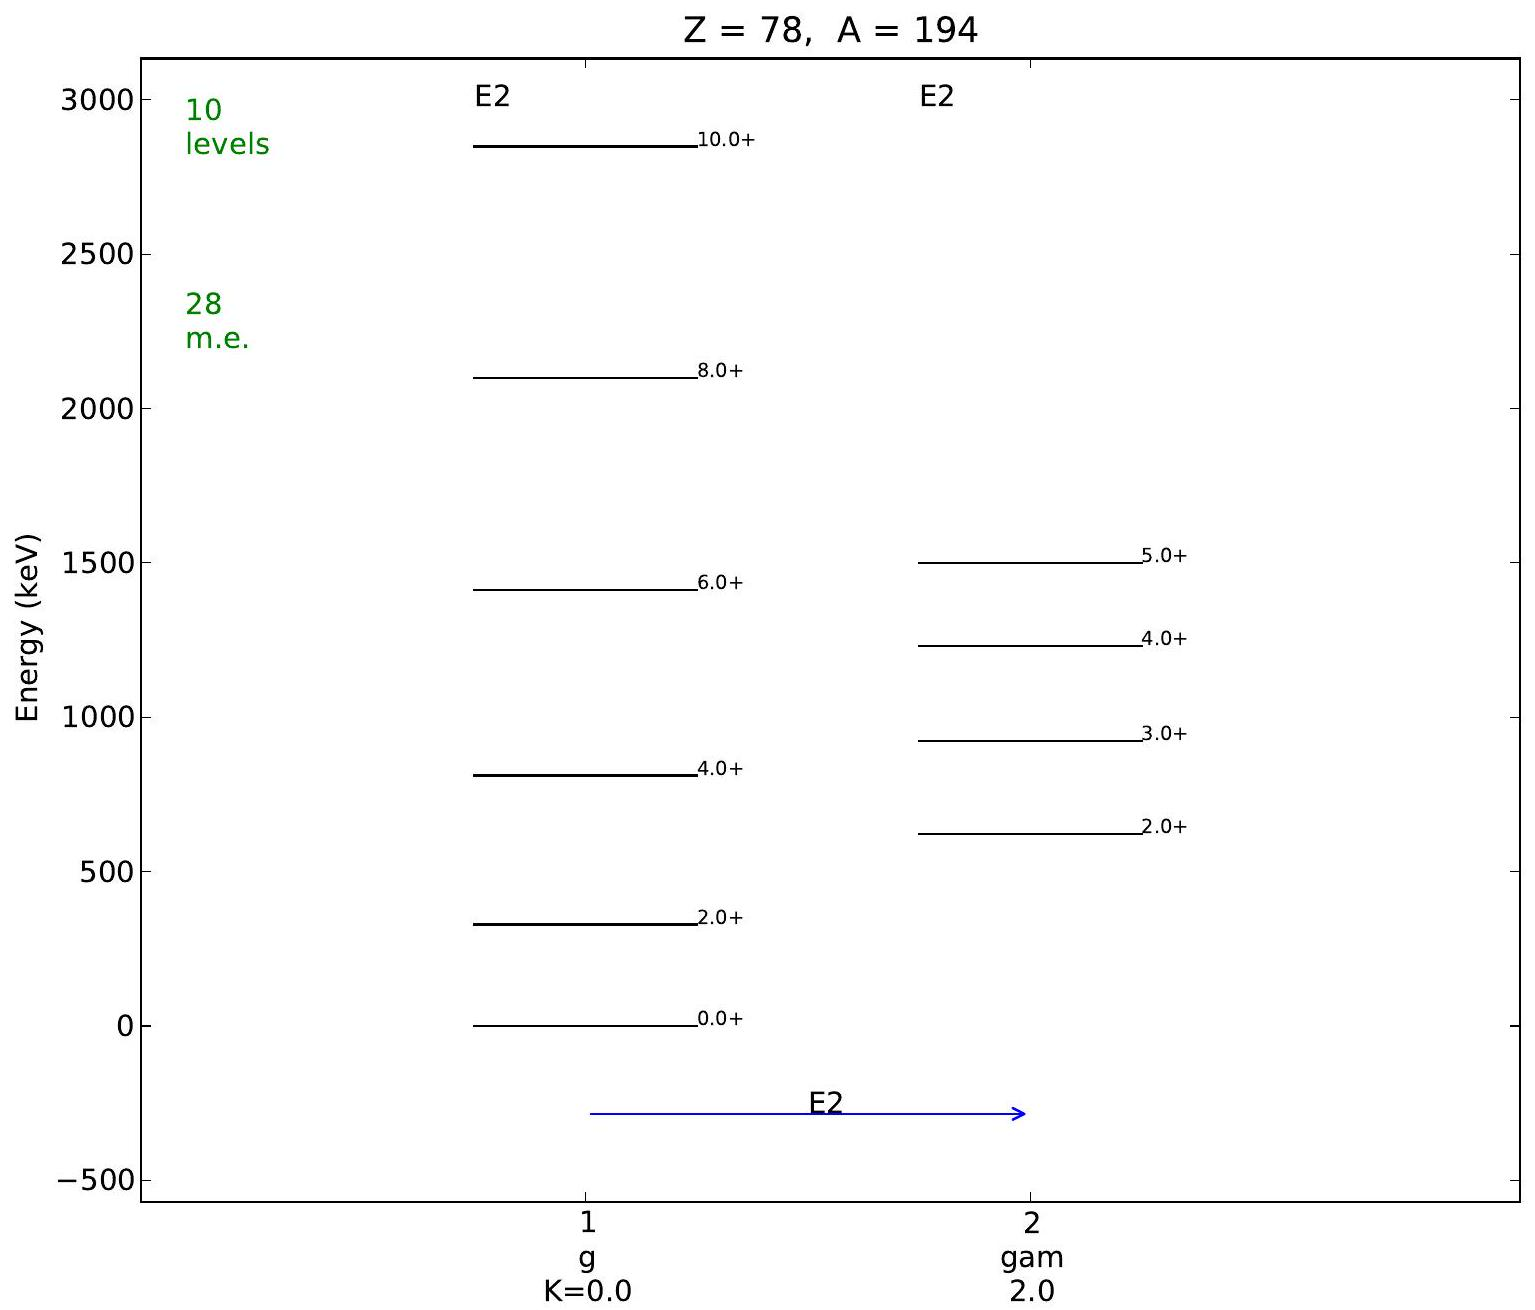
\includegraphics[max width=\textwidth, center]{2025_02_07_204a351db2d7f48b61ebg-259}

Figure 14.1: A partial level scheme of the nucleus to be investigated ( $\left.{ }^{194} \mathrm{Pt}\right)$ in the fit\_demo\_2011.tar files. The highest states in each band are "buffer" states, which are not observed in the experiment, but are required for accurate calculation of the yields of the lower levels. See section 7.14.\\
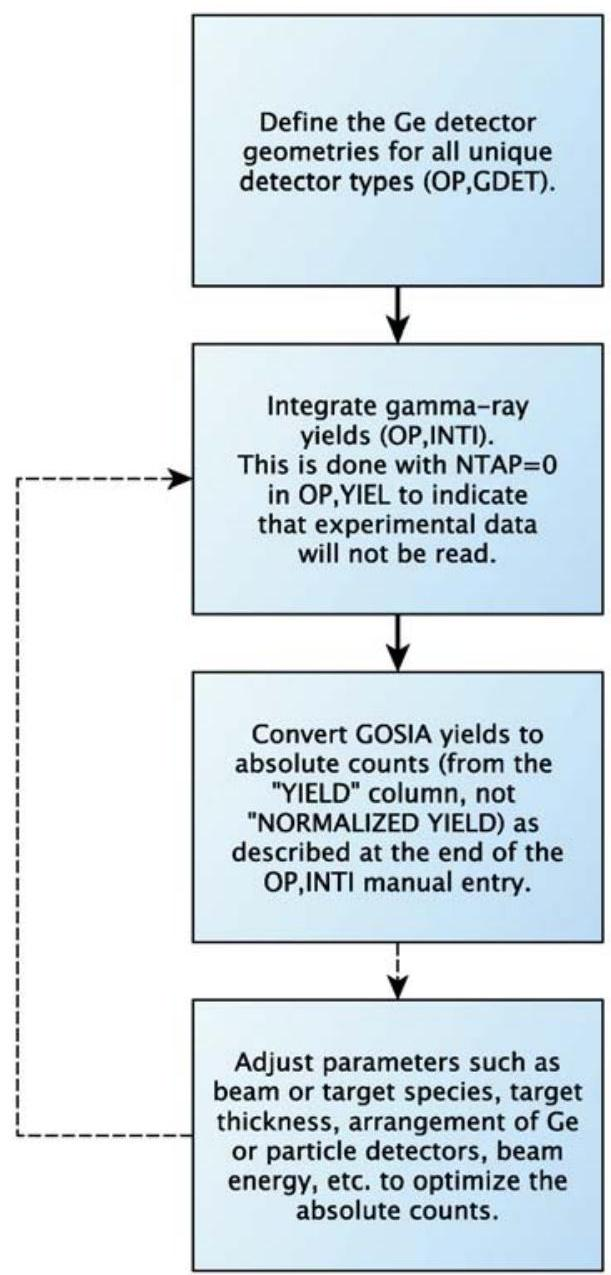
\includegraphics[max width=\textwidth, center]{2025_02_07_204a351db2d7f48b61ebg-260}

Figure 14.2: Overall flow diagram for use of Gosia.

\begin{verbatim}
    1: OP,FILE
    2: 3,3,1
    3: gosia.yld
    4: 4,3,1
    5: gosia.cor
    6: 7,3,1
    7: gosia.map
    8: 9,3,1
    9: gosia.gdt
10: 12,3,1
11: gosia.bst
12: 15,3,1
13: gosia.err
14: 22,3,1
15: gosia.out
16: 25,3,1
17: gosia.inp
18: 99,3,1
19: gosia.amp
20: 0,0,0
21: OP,GOSI
22: LEVE
23: 110.00.0
24: }212.00.3284
25: }314.00.81
26: 416.01.412
27: 5 1 8.0 2.0995
28: 6 }110.02.848
29: 71 2.00.622
30: }813.00.92
31: }914.01.2
32: }1015.01.49
33: 0000
\end{verbatim}

Figure 14.3: Simulation input file for OP,FILE\\
is defined on one line by the following quantities: index (beginning with 1 ), parity $(+/-1)$, spin, energy ( MeV ).

Note that unobservable states have been added to the level scheme in each band. These are referred to here as "buffer" states, and at least one unobservable buffer state should be added to each rotational band. The accuracy of the energies of these states is not critical, and they can be extrapolated.

The second sub-option of OP,GOSI is ME (lines $1-31$ in Figure 14.4), which defines the matrix elements, all E2 in this case. The header $2,0,0,0,0$ indicates the beginning of E2 matrix elements, and all relevant E2 reduced matrix elements are then listed with the initial and final indices in "odometer order." The following quantities describe each matrix element: initial level, final level, matrix element, lower limit, upper limit. The lower and upper limits will be used by Gosia in the fitting tutorial. Setting the lower and upper limits equal ( 1,1 in the present input) "fixes" the matrix element during a fit. The footer $0,0,0,0,0$ terminates the ME input.

The sub-option EXPT (lines 1-4 in Figure 14.5) defines the "logical" experiments to be simulated, in this case two. A "logical" experiment typically refers to detection of a scattered or recoiling particle over a particular solid angle.

Line 2: $2,78,194$\\
tells Gosia that there are two logical experiments and that the investigated nucleus (for which Coulomb excitation calculations are to be performed) has $\mathrm{Z}=78$ and $\mathrm{A}=194$.

Line 3: $22,48,145.7,30.0,6,1,0,0.0,360.0,0,1$\\
defines the "un-investigated" nucleus $\left(\mathrm{Z}=22, \mathrm{~A}=48-{ }^{48} \mathrm{Ti}\right)$, the mean beam energy in the target ( 146 MeV ), the mean laboratory scattering angle ( 30 degrees polar). The next fields define accuracy parameters for the point calculations, symmetry of the detector (azimuthal symmetry in this case), normal or inverse kinematics (irrelevant here). The last field is called "LN" and indicates that this experiment will be normalized to itself (experiment 1). The second experiment is another partition of the projectile scattering angle with a mean value of $\theta=50$ degrees. The last field describing the second experiment (line 4) is also 1 , indicating that yields for this experiment are to be normalized to those of experiment 1 during fitting. This gives greater sensitivity of the matrix elements to the yield data than if it were normalized independently using $\mathrm{LN}=2$. Obviously, it is not common that two experiments from different beam runs can be normalized in this way. Also note that these examples specify projectile detection. In the present version of GOSIA, experiments which specify target detection must be normalized independently.

Lines 5-21: The CONT(rol) block can be used to set a number of options including fixing/freeing of matrix elements, output options, the use of PIN diodes as particle detectors, etc. Line 9 tells GOSIA to use cubic-spline interpolation, which is more robust and accurate than the default Lagrange interpolation for various integrated quantities. It is recommended that the spline option always be used.

Note that a blank line is required after the flag "END," in the "PRT," (printing options) settings of CONT.

Lines 23-25: The $4^{\text {th }}$ option is OP,BRIC. This tells GOSIA to read electron conversion coefficients as needed from the .idx and .icc Bricc internal conversion data files. Before running the tutorial inputs, the two lines containing the path to the idx and icc files must be changed to point to their actual locations on the user's system.

Lines 26-48: The $5^{\text {th }}$ option is OP,YIEL, which allows the user to define the gamma-ray detector locations, internal conversion coefficients, normalization constants between experiments (relevant for normalization of one experiment to another), tabulated data (branching ratios, lifetimes, signed mixing ratios and measured matrix elements), etc. The user is referred to section 7.32 (OP,YIEL) for a detailed description. The following entries are of particular interest to the first-time user.

Lines 28-29: These are dummy arguments given in place of internal conversion data when OP,BRIC is used to generate the electron conversion data for GOSIA. Remember to change the paths and file names of the BRICC data files as necessary before running GOSIA.

Lines 30-36: These lines declare that three Ge detectors of type " 1 " in the detector file ("gosia.gdt" in this case) are positioned at polar angles 30,60 and 90 degrees and azimuthal angles 0,90 and 180 degrees, respectively, in the lab frame for both experiments 1 and 2. (Summation of a $4 \pi$ Ge array should be simulated without adding multiple detectors. Refer to the manual section on OP,GDET for the details of how to do this.)

\begin{verbatim}
    1: ME
    2: 2 0 0 0 0
    3: 1 2 1.29906265019 0.4 1.6
    4: 1 7 0.353553390593 1 1
    5: 2 -2 -1.53458635038 1 2
    6:2 3 2.0866732095 0.64142698059 2.56570792236
    7: 2 7 0.422577127364 1 1
    8: 2 8 -0.559016994375 1 1
    9: 2 9 0.365962527356 1 1
10: 3 -3 -2.0379493563 2 3
11: 3 4 2.55827606402 0.809039834956 3.23615933982
12: 3 7 0.0944911182523 1 1
13: 3 8 -0.353553390593 1 1
14: 3 9 0.628076842019 1 1
15: 3 10 -0.661437827766 1 1
16: 4 -4 0.920382602961 3 4
17: 4 5 2.36675944729 0.946572765296 3.78629106118
18: 4 9 0.184637236469 1 1
19: 4 10 -0.5 1 1
20: 5 5 -2.07237468671 1 1
21: 5 6 2.66556994992 1 1
22: 6 6 -2.29913922804 1 1
23: 7 7 1.55379719213 1 1
24: 7 8 2.05548047911 1 1
25: 7 9 1.34562784072 1 1
26: 8 9 2.01395134003 1 1
27: 8 10 1.883878977 1 1
28: 9 9 -0.795049618643 1 1
29: 9 10 1.883878977 1 1
30: 10 10 -1.30996183151 1 1
31: 0 0 0 0 0
\end{verbatim}

Figure 14.4: Example of matrix element inpu using sub-option ME

\begin{verbatim}
1: EXPT
2: 278194
3: 22, 48, 145.69999999999999, 30.0,6,1,0,0.0, 360.0, 0, 1
4: 22,48, 145.69999999999999, 50.0,6,1,0,0.0,360.0,0,1
5: CONT
6: INT,2.
7: 1,1000
8: 2,1000
9: SPL,1.
10: PRT,
11: 1,-1
12: 2,0
13: 4,0
14: 5,1
15: 11,0
16: 12,0
17: 14,0
18: 15,1
19: 16,0
20: 0,0
21: END,
21:
23: OP,BRIC
24:/home/hayes/programs/bricc/BriccFOV22.idx
25:/home/hayes/programs/bricc/BrlccFOV22.icc
26: OP,YIEL
27: 0
28: -1,0
29: 1.0
30: 33
31: 1,1,1
32: 30.0,60.0,90.0
33: 0.0,90.0, 180.0
34: 1,1,1
35: 30.0,60.0,90.0
36: 0.0,90.0, 180.0
37: 2,1
38: 3
39: 1000.0 1000.0 1000.0
: 20020.3433967 20020.3433967 20020.3433967
41: 3
42: 1000.0 1000.0 1000.0
43: 4300.199442444300.199442444300.19944244
44: 0 !NTAP
45: 0,0
46: 0,0
47: 0,0
48: 0,0
\end{verbatim}

Figure 14.5: Input for sub-option EXPT

1: OP,INTI\\
2: $20,20,141.40000000000001,150.0,20.0,40.0$\\
3: $141.40000000000001,141.85263157894738,142.30526315789473,142.7578947368421,1$ $43.21052631578948,143.66315789473686,144.1157894736842,144.56842105263158,145.02105$ 263157895, 145.47368421052633, 145.92631578947368, 146.37894736842105, 146.831578947368 $43,147.2842105263158,147.73684210526315,148.18947368421053,148.6421052631579,149.0$ 9473684210528, 149.54736842105262, 150.0

4: 20.0, 21.05263157894737, 22.105263157894736, 23.157894736842106, 24.210526315789 473, 25.263157894736842, 26.315789473684212, 27.368421052631579, 28.421052631578945, 29 . $473684210526315,30.526315789473685,31.578947368421051,32.631578947368425,33.684210$ $526315788,34.736842105263158,35.789473684210527,36.84210526315789,37.89473684210526$ , 38.94736842105263,40.0

5: $20,20,141.40000000000001,150.0,40.0,60.0$\\
6: $141.40000000000001,141.85263157894738,142.30526315789473,142.7578947368421,1$ $43.21052631578948,143.66315789473686,144.1157894736842,144.56842105263158,145.02105$ $263157895,145.47368421052633,145.92631578947368,146.37894736842105,146.831578947368$ $43,147.2842105263158,147.73684210526315,148.18947368421053,148.6421052631579,149.0$ 9473684210528, 149.54736842105262, 150.0

7: $40.0,41.05263157894737,42.10526315789474,43.157894736842103,44.2105263157894$ $73,45.263157894736842,46.315789473684212,47.368421052631575,48.421052631578945,49$. $473684210526315,50.526315789473685,51.578947368421055,52.631578947368425,53.6842105$ 26315788, 54.736842105263158, 55.789473684210527, 56.84210526315789, 57.89473684210526, 58.94736842105263,60.0

8: 20\\
9: $\quad 141.40000000000001,141.84999999999999,142.31,142.75999999999999,143.21000000$ 000001, 143.66, 144.12, 144.56999999999999, 145.02000000000001, 145.47, 145.93000000000 $001,146.38,146.83000000000001,147.28,147.74000000000001,148.19,148.63999999999999$ , 149.09, 149.55000000000001, 150.0

10: $8.5786700000000007,8.57728,8.5756599999999992,8.5740099999999995,8.572449999$ 9999999, 8.5707699999999996, 8.5691299999999995, 8.5674399999999995, 8.5657599999999992 , 8.5640400000000003, 8.5623199999999997, 8.5605100000000007, 8.5587300000000006, 8.556 $9400000000009,8.5551100000000009,8.5533000000000001,8.5514500000000009,8.5495800000$ 000006, 8.5476799999999997, 8.5458099999999995

11: 5050\\
12: 20\\
13: 141.40000000000001, 141.84999999999999, 142.31, 142.75999999999999, 143.21000000 000001, 143.66, 144.12, 144.56999999999999, 145.02000000000001, 145.47, 145.93000000000 $001,146.38,146.83000000000001,147.28,147.74000000000001,148.19,148.63999999999999$ , 149.09, 149.55000000000001, 150.0

14: $8.5786700000000007,8.57728,8.5756599999999992,8.5740099999999995,8.572449999$ 9999999, 8.5707699999999996, 8.5691299999999995, 8.5674399999999995, 8.5657599999999992 , 8.5640400000000003, 8.5623199999999997, 8.5605100000000007, 8.5587300000000006, 8.556 9400000000009, 8.5551100000000009, 8.5533000000000001, 8.5514500000000009, 8.5495800000 000006, 8.5476799999999997, 8.5458099999999995

15: 5050\\
16: OP,EXIT\\
17:

Figure 14.6: A sample OP,INTI input file.

Line 37: The normalization transition to be used when fitting matrix elements to data is the level $2 \rightarrow$ level $1\left(2^{+} \rightarrow 0+\right)$ transition in the yrast sequence.

Lines 38-43: The upper limits and normalization constants are given here. These are only necessary for fitting and error calculations; for other processes dummy values may be entered. Note that it is assumed here that all $\gamma$-ray yield data are corrected for the relative efficiency of each Ge detector, hence the normalization constants are equal for all three Ge detectors in each experiment. Only differential Rutherford cross section and $\sin (\theta)$ term factors are included in this case. The normalization constants are calculated according to the formula in the OP,YIEL section of the manual.

Line 44: NTAP is set to 0 , which tells Gosia that no experimental yields are to be read from disk. Obviously, experimental data are not used to simulate yields.

Lines 45-48: Spectroscopic data will be entered here, to be included in the $\chi^{2}$ fit, but they are ignored during simulation (integration).

The final option used is OP,INTI (Figure 14.6), which integrates the point calculations over the particle scattering angles and the beam energy range as the projectile traverses the target. Lines 2-4 and 8-11 correspond to experiment 1.

Line 2: $\quad 20,20,141.4,150.0,20.0,40.0$\\
indicates that 20 energy meshpoints and 20 polar scattering angle meshpoints will be provided by the user. The energy range as the beam traverses the target is $141.4-150 \mathrm{MeV}$, and the particle detector covers the laboratory scattering angle range 20-40 degrees. In the present version of Gosia, the energy range must be calculated by the user from tabulated stopping power data, while the RACHEL interface calculates them automatically.

Lines 3-4: The beam energy and $\theta_{\text {scat }}$ meshpoints are entered for the integration. Both of these sets of meshpoints should meet or exceed the integration range. It is wise to increase or decrease the number of meshpoints at least once in a test calculation to make sure that convergence has been achieved, or use the optional accuracy tests in RACHEL.

Lines 5-7: Similar entries are given for experiment 2.\\
Lines 8-10: Stopping power data for the beam and target combination are entered for experiment 1.\\
Note that RACHEL calculates all of the OP,INTI data above automatically, using Zeigler's stopping power tables for $Z_{\text {targ }}<93$ in the present version.

Line 11: The number of subdivisions in energy and scattering angle to be used for the fast interpolation between meshpoints in experiment 1. When starting a new calculation it is wise to halve or double the number of subdivisions at least once to make sure that convergence is achieved. Refer to the troubleshooting section in this chapter. (RACHEL selects an appropriate number of meshpoints and subdivisions to ensure convergence of the integrated yields.)

Similar stopping power and subdivision lines for experiment 2 conclude the input data, and the line OP,EXIT terminates the input. (Nothing below OP,EXIT will be processed.)

In this example, the Ge detector definitions file gosia.gdt has already been provided. (The fitting tutorial in this section gives an example of how to create a detector file.) In order to produce simulated yields, Gosia only needs to be told to execute the gosia.inp input file using the command

\begin{verbatim}
gosia < gosia.inp
\end{verbatim}

The following output should be generated

\begin{verbatim}
OPENED gosia.out
IO-num = 22 UNKNOWN FORMATTED
etc.
\end{verbatim}

When the system prompt is returned, an output file gosia.out will be present. Among other data, the simulated, integrated yields appear at the end of the input. The yield output looks like the following.

\begin{verbatim}
    INTEGRATED YIELDS
    EXPERIMENT 1 DETECTOR 1
ENERGY RANGE 141.400--- 150.000 MEV SCATTERING ANGLE RANGE 20.000--- 40.000 DEG
    NI NF II IF YIELD NORMALIZED YIELD
    6 5 10.0 8.0 0.48736E-09 0.86376E-11
    ********* END OF EXECUTION ***********
\end{verbatim}

The cross section for measuring the gamma-ray transition from state 6 to state 5 in a nearly perfect blackbody detector can be obtained from the line of output quoted above. In the YIELD column, GOSIA gives a differential cross section, which is integrated over the particle detector solid angle and the energy range in the target, but not over the Ge detector solid angle. In the present example, this quantity is $d \sigma / d \Omega_{\gamma}=(0.48736 E-09) m b \bullet(m g / c m 2)(1 / s r)$, where the units $m g / c m 2$ and $(1 / s r)$ refer to integration over the target thickness and the solid angle subtended by the Ge detector, respectively.

The gosia.gdt file provided with this demonstration input represents a Ge detector of 7 cm diameter placed with its face 25 cm from the target position. Hence, it subtends a solid angle of 0.061 sr . The energy range of integration was chosen for a $1 \mathrm{mg} / \mathrm{cm}^{2}$ target thickness, so the absolute cross section for scattering of the beam into the particle detector and emission of the $10^{+}$to $8^{+} \gamma$ ray into the Ge detector is then $\sigma_{p \gamma}=2.97290 E-11 \mathrm{mb}$. This is obviously not measurable and indicates that more buffer states (see above) probably are not needed.

Note that this is not a point calculation of the mean cross section at the mean beam energy, but rather, it is integrated over the energy range of the beam in the target. Refer to section 7.12 of this manual to convert this cross section to absolute counts.

The RACHEL interface both constructs the OP,INTI section and interprets the output with more readily available input quantities, such as the target thickness in $\mathrm{mg} / \mathrm{cm}^{2}$, the initial beam energy, etc. Absolute counts can also be calculated in the GUI, with optional Gaussian scatter to better simulate real data.

\subsection*{14.3.2 Fitting Matrix Elements to Gamma-Ray Yield Data}
This section describes the use of a series of sample inputs to fit matrix elements to simulated experimental data, which have been provided in the fit\_demo\_2011.tar archive. Four E2 reduced matrix elements in the yrast sequence are fitted to the simulated data plus a (fictitious) lifetime measurement. The lifetime measurement is needed in this case to constrain the normalization for a few-state system. Without any spectroscopic data, the matrix elements, which are strongly correlated with the overall normalization of the few data, may run away, giving a good fit, but meaningless physical quantities. The level scheme is the same as the one in the previous demonstration, that is Fig 14.1.\\
(Data for some multi-step Coulomb excitation experiments, such as strongly-deformed nuclei excited by collisions with other heavy nuclei, can be self-normalized without including spectroscopic data.)

The simulated problem can be used as a model for the basic procedure used to analyze real data, even though a real problem might involve more sophistication, such as axially asymmetric particle detectors (of arbitrary shape), data from user-defined Ge detector "clusters," choices regarding the normalization of one data subset to another, data from multiple beam and target combinations, data from unresolved doublets, inverse scattering kinematics, etc. A flowchart of the general procedure to define the Ge detector(s), fit matrix elements to the data and estimate the errors in the fitted matrix elements is given in Figures 14.7 and 14.8.

The demonstration is run using a set of inputs and related files in the fit\_demo\_2011.tar archive on the Gosia website. Each step of the demonstration is run with a different *.inp file. In practice it is probably better to use the same input file for all or most steps to prevent accidental inconsistencies between steps. In that case, the files should be modified for each step using a text editor such as emacs or vi, paying attention to delimiters, spacing and capitalization. Each step in the procedure is executed by typing

\begin{verbatim}
gosia < gosia.inp
\end{verbatim}

The relevant portion of the input is described below for each step, but the novice user should refer to the manual entries in Chapter 7 for complete details of the records and fields required for a particular Gosia option, e.g. OP,GOSI or OP,INTI etc. This demonstration includes two iterations of the fitting procedure to make sure that the correction factors for the point approximations used in the fit are sufficiently accurate at the final minimum point in the chi-squared surface. At each step, move into the directory named under the section heading. It will be necessary to make only one modification to each input file: the user must change the two OP, BRIC file name lines in a text editor, so that they point to the correct BRICC data files on the user's system. Do this before issuing the command to run GOSIA, with the exception of the Ge detector definition example.

A set of simulated gamma-ray yield data is provided for the user in the file gosia.yld in the appropriate directories. In practice, this file would be typed by the user according to the format in section 7.32.\\
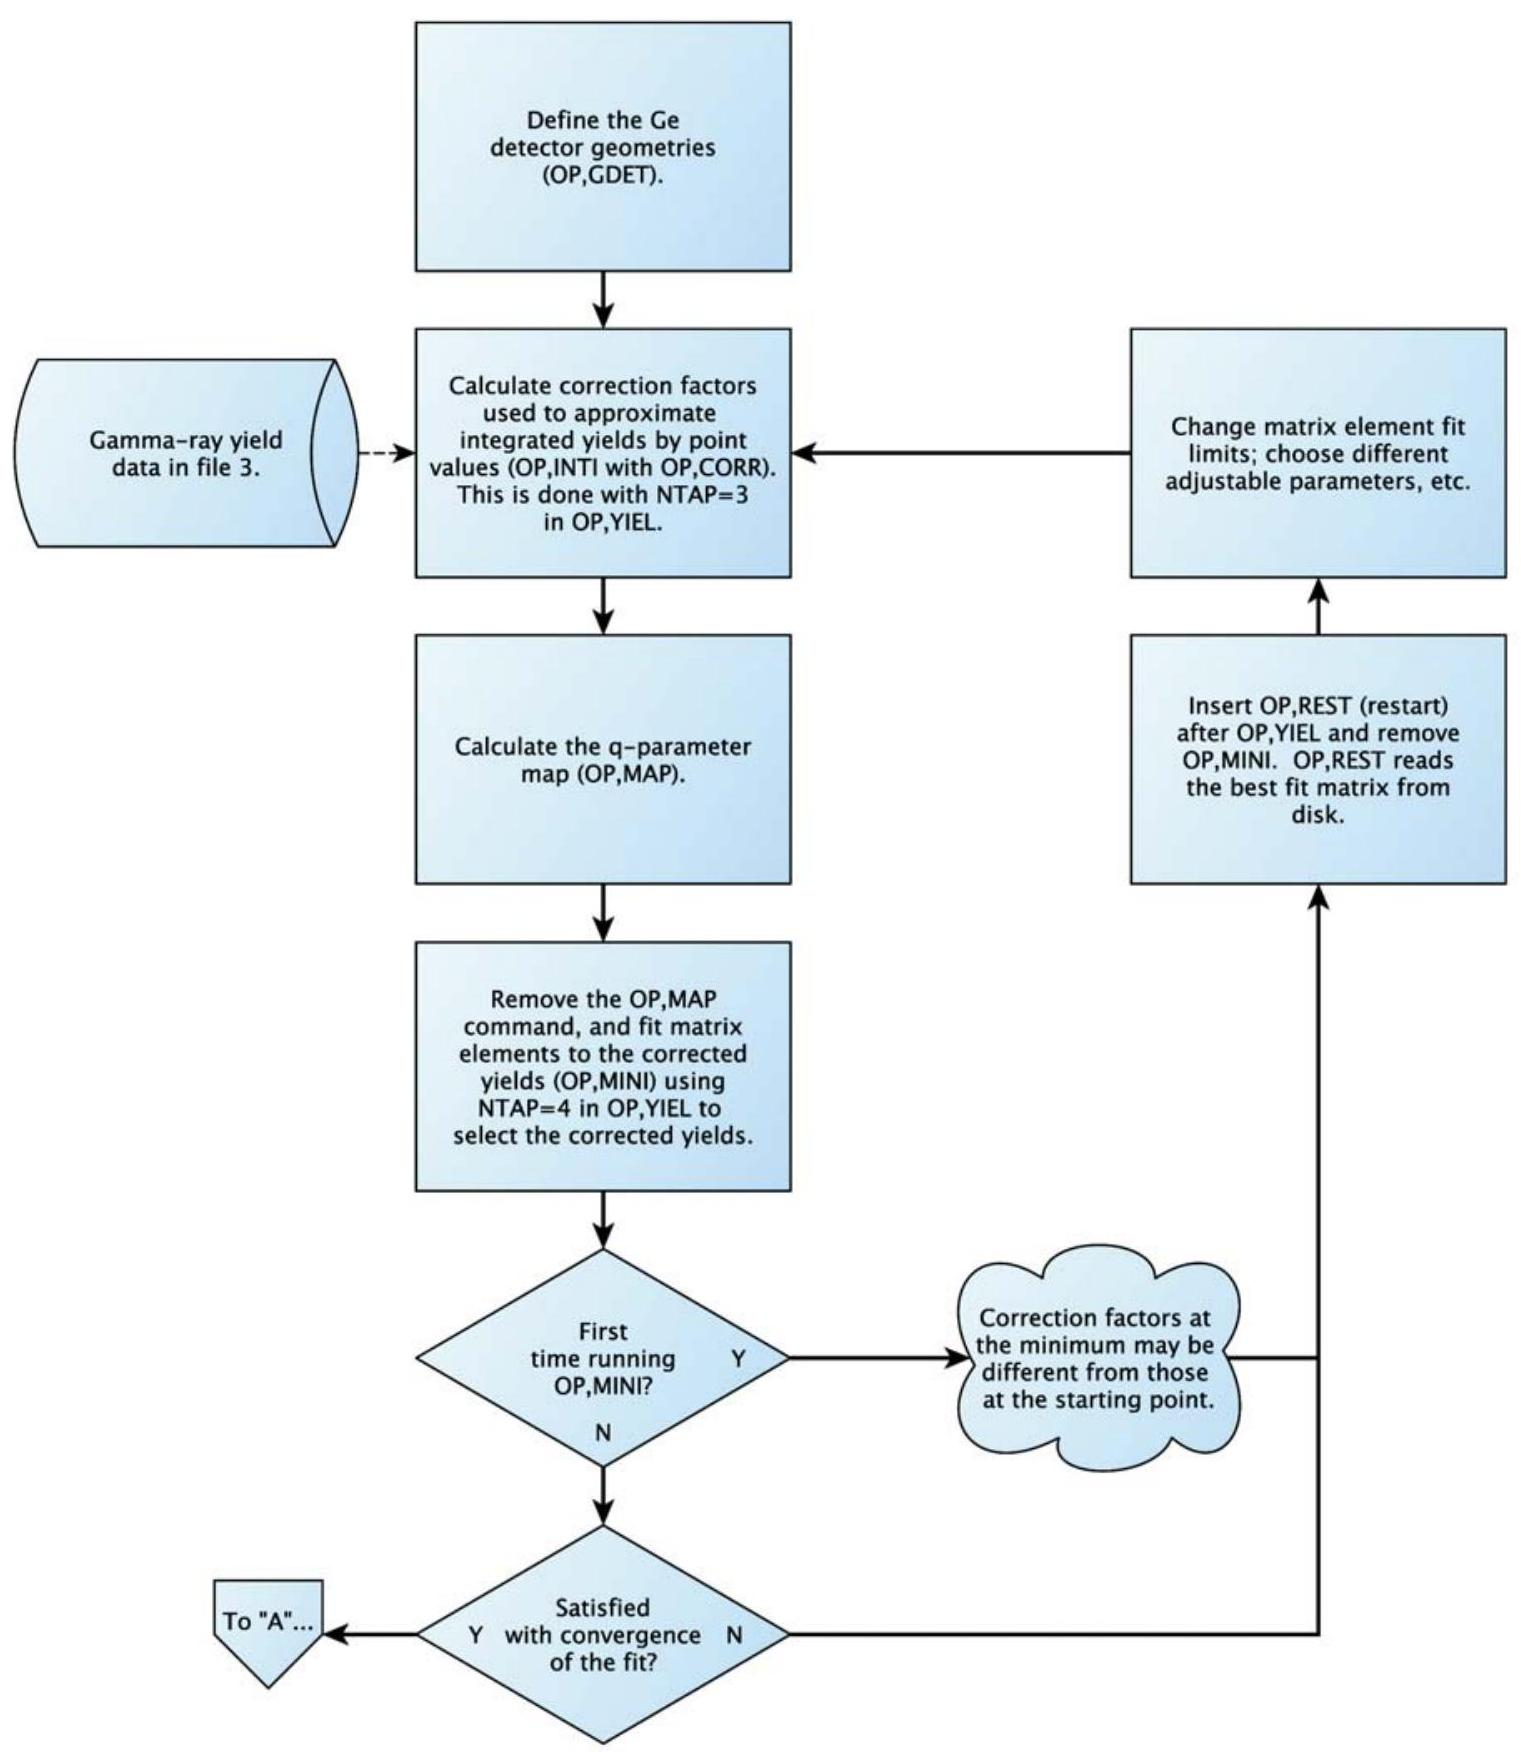
\includegraphics[max width=\textwidth, center]{2025_02_07_204a351db2d7f48b61ebg-268}

Figure 14.7: Flow diagram for running a Gosia minimization job; part 1.\\
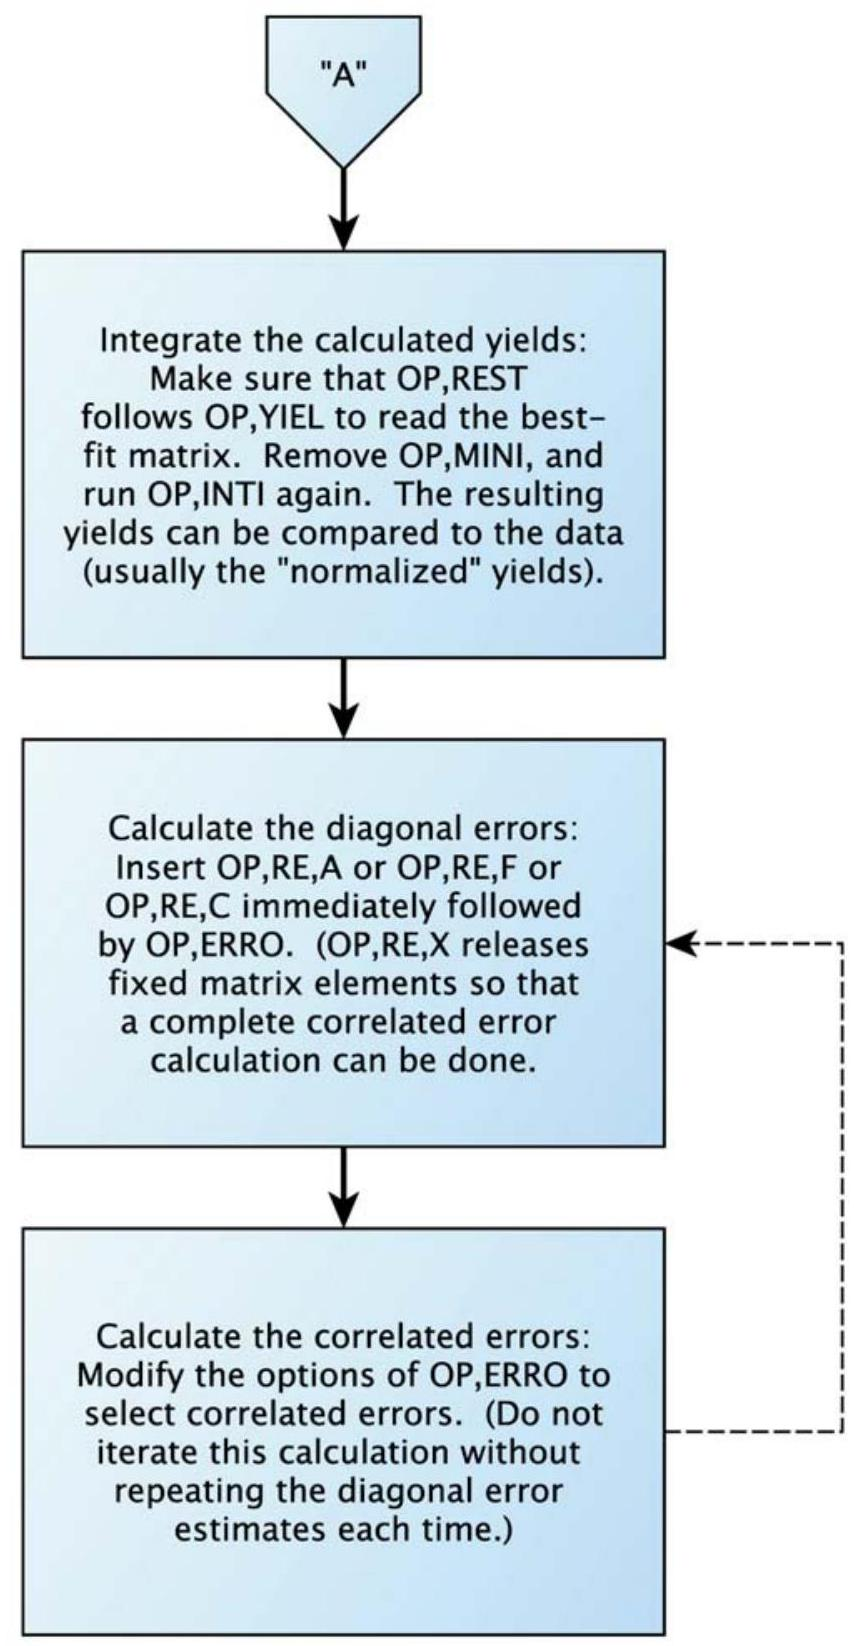
\includegraphics[max width=\textwidth, center]{2025_02_07_204a351db2d7f48b61ebg-269}

Figure 14.8: Flow diagram for running a Gosia minimization job; part 2.

\section*{1. Define the Ge detector(s)}
(Directory "1-gdet" in the directory tree in the .tar archive)\\
In Gosia, detectors are considered to be "physically different" if they have different geometry (crystal length, crystal radius, etc.), if they are placed at different distances from the target position, or if they are fitted with different absorbers. Two identical Ge detectors placed at different distances from the target need to be defined separately, but two identical detectors that only differ by their angular position in space (and their efficiencies) should be defined as the same "type." In this demonstration, one detector type is defined and named type "1."\\
Refer to the file "gosia.inp" in this directory. In OP,FILE the three necessary files for OP,GDET are defined. The general output will be written to gosia.out, but the coefficients for the angular attenuation (Sections 7.10 and 4.4 ) will be written to "gosia.gdt" for use by Gosia in steps $2-8$.

OP,GDET has three lines. The first line is the detector type, 1. The second line\\
0.1,3.55,8.0,25.25\\
defines a Ge crystal with an inactive core of radius 0.1 cm , outer radius of 3.55 cm and length 8.0 cm , placed 25.25 cm from the target. (The angular position(s) in space of all detectors of this type will be defined in the next step.)\\
To execute the input, issue the command

\begin{verbatim}
gosia < gosia.inp
\end{verbatim}

in the directory 1-gdet. The output file gosia.out contains verbose output, some of which is selected by the user in the sub-option PRT of CONT. Error messages will also be written to this file. The Ge detector file gosia.gdt is created with the following records.

\begin{verbatim}
1
25.250000000000000
5.00000007450580597E-002
0.99589155199729673 2.21592661065883219E-002 0.99514773792810363
0.98770897800534885 2.21737615543087588E-002 0.98549026565841702
0.97552055810707139 2.21956101867980850E-002 0.97112111660820433
0.95942780694782859 2.22249408117792362E-002 0.95217917281887521
0.94726773962281452 2.22773442679664278E-002 0.937944497620683592
0.91609475810652463 2.23068006995633186E-002 0.90134856707041400
0.88921232048412568 2.23598366183371221E-002 0.86994669878926978
0.85913750492580931 2.24213784125499860E-002 0.83493976674575587
\end{verbatim}

In subsequent steps the detector will be referred to as type " 1 " (line 1 ). The second line is the distance from the target, and the third line is the energy offset $E_{0}$ of equation 6.37. The remaining lines are the values $C_{1}, C_{2}$ and $Q_{k}$ of equations 6.37 and 4.35 for each order $k=1 \ldots 8$.\\
Now, attaching the file gosia.gdt to an input (OP,FILE) will allow GOSIA to find the angular attenuation factors when detector type " 1 " is called.

\section*{2. Calculate the Correction Factors for the Point Approximation}
(Directory "2-corr" in the directory tree in the .tar archive)\\
Now a set of correction factors needs to be calculated so that GOSIA can use a point approximation for the scattering angle range of the particle detector to speed up the fit process. The input used is nearly identical to the one described in the simulation demo; refer to section 14.3 .1 for a description. One difference is that OP,CORR is added just after OP,INTI. OP,CORR takes no arguments, but tells GOSIA to compare the predicted yields it has just integrated to the corresponding point calculations and use the quotient as one of the two necessary correction factors. Notice that NTAP is labeled in the input file under OP,YIEL. In this step NTAP is set to 3 , the file number of the gosia.yld file, which contains the experimental yields. (The file number for $\gamma$-ray yield data is not open to the user's choice. It must always be 3.) The experimental yields in this file are read by Gosia because NTAP $=3$, and these yields are "corrected" to be consistent with the point approximation. The results are then written to file 4, gosia.cor, which has a similar format to gosia.yld. In the steps that follow, these corrected yields will be read by GOSIA and compared to the calculated yields to calculate the $\chi^{2}$ statistic.

Make sure to move into the directory 2-corr, and run GOSIA with the same command as in the previous step.

\section*{3 Generate the q-Parameter Map - Fit the Adjustable Matrix Elements}
(Directory "3-fit" in the directory tree in the .tar archive)\\
In order to ensure that the set of adjustable parameters has been overdetermined, and because of the lack of sensitivity of the predicted yields to the static moments in multi-step processes, the static moments which will be fit are coupled to the $\Delta I=2$ E2 matrix elements directly below in the level scheme. This is done for each static moment by flagging the second field (the index of the final state) in the ME section with a negative sign and replacing the upper and lower limits with the indices of the "chosen master" matrix element. This can be seen in the example input in Figure 14.4 and in the gosia.inp file for this step. This is a useful tactic when there is insufficient data to fit some matrix elements individually, but the ratio of two matrix elements can be calculated, as in the matrix elements of a rotational band with a constant intrinsic quadrupole moment $Q_{0}$. The "q-parameter" map (Section 6.2 ) is created during the same calculation by adding the single line OP,MAP inserted at the end of OP,YIEL (just before OP,MINI in this case). Any time the ranges are changed by the user, over which matrix elements are allowed to vary, OP,MAP should be run again.\\
File number 7 is assigned to gosia.map. After execution of this step, it should contain the q-parameter map appropriate for this fit.

In this, and the following fitting and error calculation steps, the variable NTAP in OP, YIEL is set to 4, so that GOSIA uses the "corrected yields" to calculated chi-squared.\\
OP,INTI is not necessary, since the corrected yields will be compared to the point yields at each step of the minimization.

OP,MINI is inserted following OP,YIEL. There are a number of user controls (maximum number of iterations, minimum derivative of the matrix element vector to terminate the fit, etc.) that define the criteria for convergence and choices of the search method in the parameter space. The best choice will be case-dependent. Refer to section 7.18.\\
Issue the command

\begin{verbatim}
gosia < gosia.inp
\end{verbatim}

The progress of $\chi^{2}$ search will be sent to standard output until GOSIA satisfies the convergence criteria, reaches the maximum number of iterations chosen by the user, or meets some other termination criterion. The output should look similar to the following.

\begin{verbatim}
OPENED gosia.out
IO-num = 22 UNKNOWN FORMATTED
OPENED gosia.inp
IO-num = 25 UNKNOWN FORMATTED
OPENED gosia.gdt
IO-num = 9 UNKNOWN FORMATTED
OPENED gosia.map
IO-num = 7 UNKNOWN FORMATTED
OPENED gosia.cor
IO-num = 4 UNKNOWN FORMATTED
OPENED gosia.bst
IO-num = 12 UNKNOWN FORMATTED
*** CHISQ= 0.313370E+02 ***
*** CHISQ= 0.204481E+00 ***
\end{verbatim}

More details of the progress toward the minimum are given in the gosia.out file following the calculation. For instance, if the search hit a limit in one or more matrix elements this will be reported as a warning to indicate that either the range is too narrow, or a matrix element is not sensitive to the data. At the conclusion of the fit, the best set of matrix elements are written to file 12 , gosia.bst. In the second iteration (steps 4 and 5), GOSIA will begin at this new starting point in the parameter space. Steps 4 and 5 are a\\
repeat of steps 2 and 3 with point-correction factors calculated for a matrix (presumably) closer to the true $\chi^{2}$ minimum.

\section*{4. Re-calculate Correction Factors at the Minimum}
(Directory "4-iterate-corr" in the directory tree in the .tar archive)\\
NTAP is set to 3 again in this step, so that the original $\gamma$-ray yields will be read and new correction factors generated from them.\\
This step is identical to step 2, except that the file 12 containing the best set of matrix elements fitted so far, gosia.bst, is attached in OP,FILE and OP,REST is inserted immediately before OP,INTI. OP,REST takes only the arguments 0,0 in this example, which tells GOSIA to use all of the best-fit matrix elements without exception. As in step 2, the corrected yields are written to disk at the conclusion of the calculation. They will be attached as input again in step 5 .

\section*{5. Fit the Matrix Elements Again from the New Starting Point}
(Directory " 5 -iterate-fit" in the directory tree in the .tar archive)\\
Since the ranges of the matrix elements have not changed in this example, it is not necessary to recalculate the q-parameter map, but OP,MAP requires little time, and it is good practice to make sure that the qparameters are correct for the current fit.

This minimization step is identical to the first (step 3), except that OP,REST is included, telling GOSIA to overwrite the values of the matrix elements in the input with those at the conclusion of the last fit. The fit will resume at this starting point, and with the new correction factors, until the user's convergence criteria are satisfied again.\\
After running GOSIA again, the output file indicates that the convergence conditions were met in a few steps with little change in the matrix. This indicates that the initial guesses at the matrix elements were close enough to the minimum that the correction factors for the point approximation are valid at the final minimum. If the new minimum were significantly different (if $\chi^{2}$ improved by $\sim 1 / N$, where $N$ is the number of degrees of freedom) then steps 5 and 6 could be repeated again.

This is a demonstration problem. In practice, a global fit of the parameters necessary to describe the populations of all bands and states should be performed and included in the error analysis. This can be done in terms of model parameters by coupling more matrix elements to one "master." It is left to the physicist to determine what parameters should be included in the fit and error calculations, so that reasonable uncertainties and best values are calculated.

\section*{6. Estimate the Diagonal Errors}
(Directory "6-diagonal-error" in the directory tree in the .tar archive)\\
The diagonal errors are calculated individually for each matrix element which was varied in the fit. Correlations are not considered in this step. This is roughly equivalent to varying only one matrix element at a time to search for the limits where the width of the $\chi^{2}$ surface is given by $\chi^{2}=\chi_{\min }^{2}+1$, i.e., in the parameter space on a plane passing through the minimum parallel to the matrix element's axis.\\
Usually, OP,RE should be used to release the fixed matrix elements and optionally to release couplings between them. OP,RE,X is placed immediately before the OP,ERRO command. The use of OP,RE,X is case-dependent and left to the user to decide on which parameters should be included in the diagonal and correlated error calculations.

The OP,ERRO option takes 6 arguments. By changing these arguments (and iterating the diagonal and correlated error steps), the user can decide which matrix elements to include in the error estimate, activate the sum-rules calculation if desired, etc. In this case, a simple diagonal error will be calculated for each of the matrix elements designated as adjustable parameters in the ME section. The $6^{t h}$ argument, RMAX, is the largest floating point number available on the user's platform. In this case it is set to 1.0 E308, but it should be adjusted to the maximum float value on the system where it is run. (Note that the RACHEL GUI selects this value automatically.) If Gosia reports the error "TOO FAR FROM THE MINIMUM TO CARRY OUT THE ERROR ESTIMATION!" in the output file (gosia.out), the user should check that RMAX is set correctly, since this error calculation has been tested and found to converge.

Gosia reads the final set of matrix elements of the fit procedure from file 12 (gosia.bst) and performs the diagonal error calculation. The output file contains the following text:

\begin{verbatim}
DIAGONAL ESTIMATED ERRORS
INDEX NI NF ME AND ERRORS
\end{verbatim}

$1121.28458(-0.00632,0.01553) \ldots \ldots-0.5,1.2 \mathrm{PC}$\\
etc., which gives the (lower, upper) diagonal errors. These are also written to file number 15 (gosia.err) for use in the next step - the correlated error calculation.

\section*{7. Estimate the Correlated (Total) Errors}
(Directory "7-correlated-error" in the directory tree in the .tar archive)\\
The diagonal error calculation (step 6) must be run before the correlated error each time correlated errors are calculated. Failing to do so will cause the correlated errors to be overestimated by a factor of $\approx 2$ each time.

This input is very similar to the diagonal error input, except that argument 1 (IDF) of OP,ERRO is changed to 1 to select the correlated error and IREP set to 1 , which tells Gosia to read the diagonal errors from disk first.

Again, the output file contains a report of the errors. These are the correlated errors- the total errorswhich are the widths of projections on each matrix element's axis of the minimum at the $c h i^{2}=c h i_{\text {min }}^{2}+1$ level. The output file reports the correlated errors in the same format as the diagonal errors. (In this example, all matrix elements were not varied, so the user should suspect that the completely correlated errors may be larger. If there is insufficient data to vary all matrix elements, then several sets can be left coupled to one master, for example preserving the Alaga rule or the rotor model.)

If the correlated error calculation finds a better minimum, the final set of matrix elements can be found on file 17. If it is desired to reload this matrix, file number 17 can be copied to file 12 , gosia.bst. The OP,REST command will then re-read them in subsequent iterations.

Figure 14.9 shows the "true" $B(E 2)$ values used to simulate the data and the best-fit values with the correlated errors. When fits are performed on simulated data transformed into absolute counts (manual section 7.13 , OP,INTI) for a planned beam run, the correlated error calculations can be used as an estimate of the expected precision in the proposed experiment. The RACHEL interface calculates predicted measured counts with simulated statistical errors to aid in planning. It also fits parameters to simulated data with or without random scatter in the data.\\
8. Integrate the Reproduced (Calculated) Yields Using the Final Set of Matrix Elements (Directory "8-integrate" in the directory tree in the .tar archive)\\
The user can see how good the fit is by comparing the calculated yields at the chi-squared minimum to the experimental data. This is done by running an input very similar to the simulation with the addition of OP,REST immediately before OP,INTI and file 12 (gosia.bst) attached (copied from file 17, if the correlated error estimate generated a better matrix.

Run the gosia.inp file in this directory. Gosia reads the best set of matrix elements from file 12 (gosia.bst) and integrates the yields. The yields in the output file (22, gosia.out) can be compared directly to the experimental data, observing the appropriate normalization. The yields for each experiment are normalized to the chosen transition (NS1, NS2 in OP,YIEL) in the column "NORMALIZED YIELD." Absolute counts can be calculated from the "YIELD" data as in section 7.13.

Figure14.10 shows the measured (simulated) yield data and the predicted yields for the yrast line. Note that without any random scatter of the data the $\chi^{2}$ value is extremely small.

\subsection*{14.4 Accuracy and speed of calculations}
This section discusses accuracy in the integration of gamma-ray yields. Integration accuracy affects calculated yields as well as minimization (through the correction factors calculated by OP,INTI and OP,CORR). Accuracy in the chi-squared minimization process is discussed in detail in chapter 6.

While the integrated yields do not present convergence issues in the majority of calculations, even with default accuracy settings, special attention should be given to the following:

\begin{enumerate}
  \item High transition energies ( $\sim 1 \mathrm{MeV}$ in a single step). In these cases (and in any case where speed is not a problem), it is recommended that the INT option in the CONT (control) block be used to set $I S=1000$ for maximum accuracy. Refer to sections 6.3 and 7.3 regarding the adiabaticity and eccentricity limits of GOSIA. (The RACHEL interface can test for problem transitions of this type.)\\
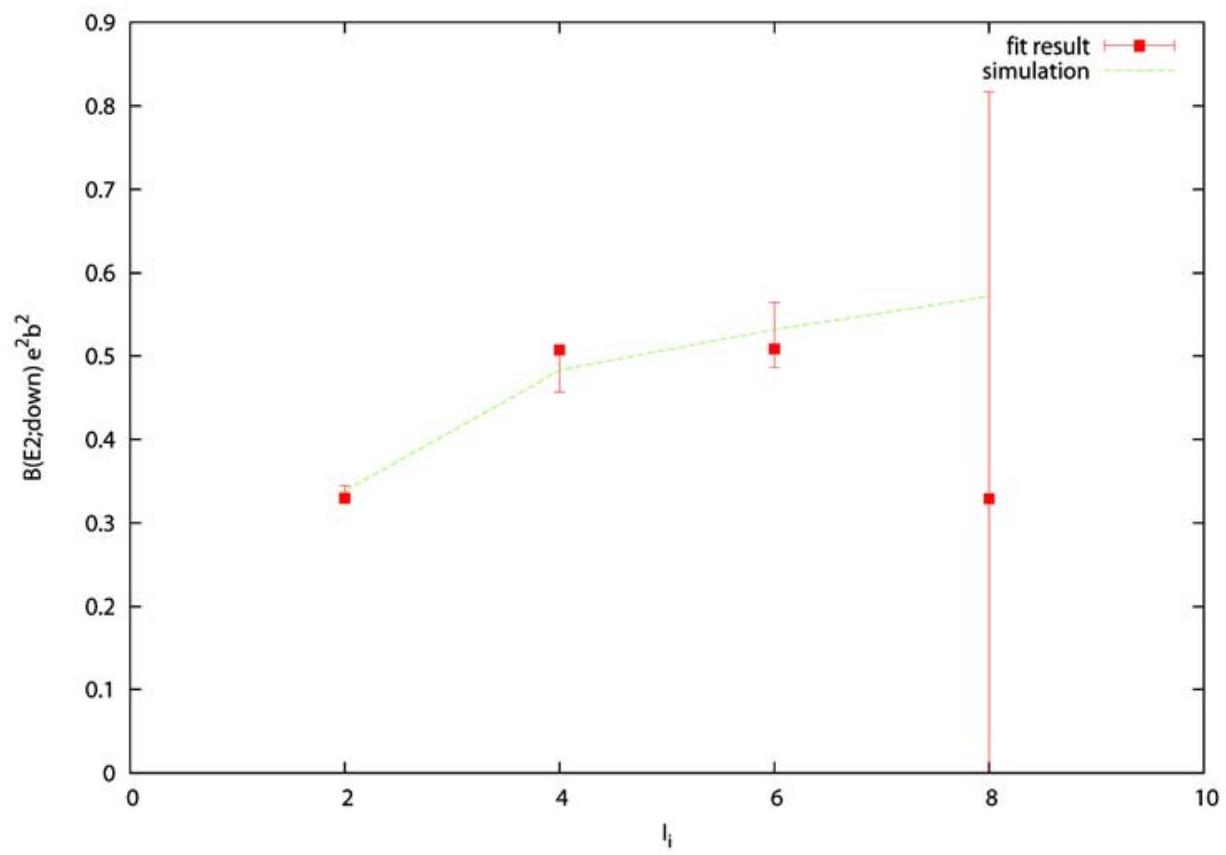
\includegraphics[max width=\textwidth, center]{2025_02_07_204a351db2d7f48b61ebg-274}
\end{enumerate}

Figure 14.9: A example of a fit to simulated data for a ground-state band. The assumed matrix elements used to simulate the data are shown by the dashed green line while the red points plus errors correspond the the best fit matrix elements plus their correlated errors.\\
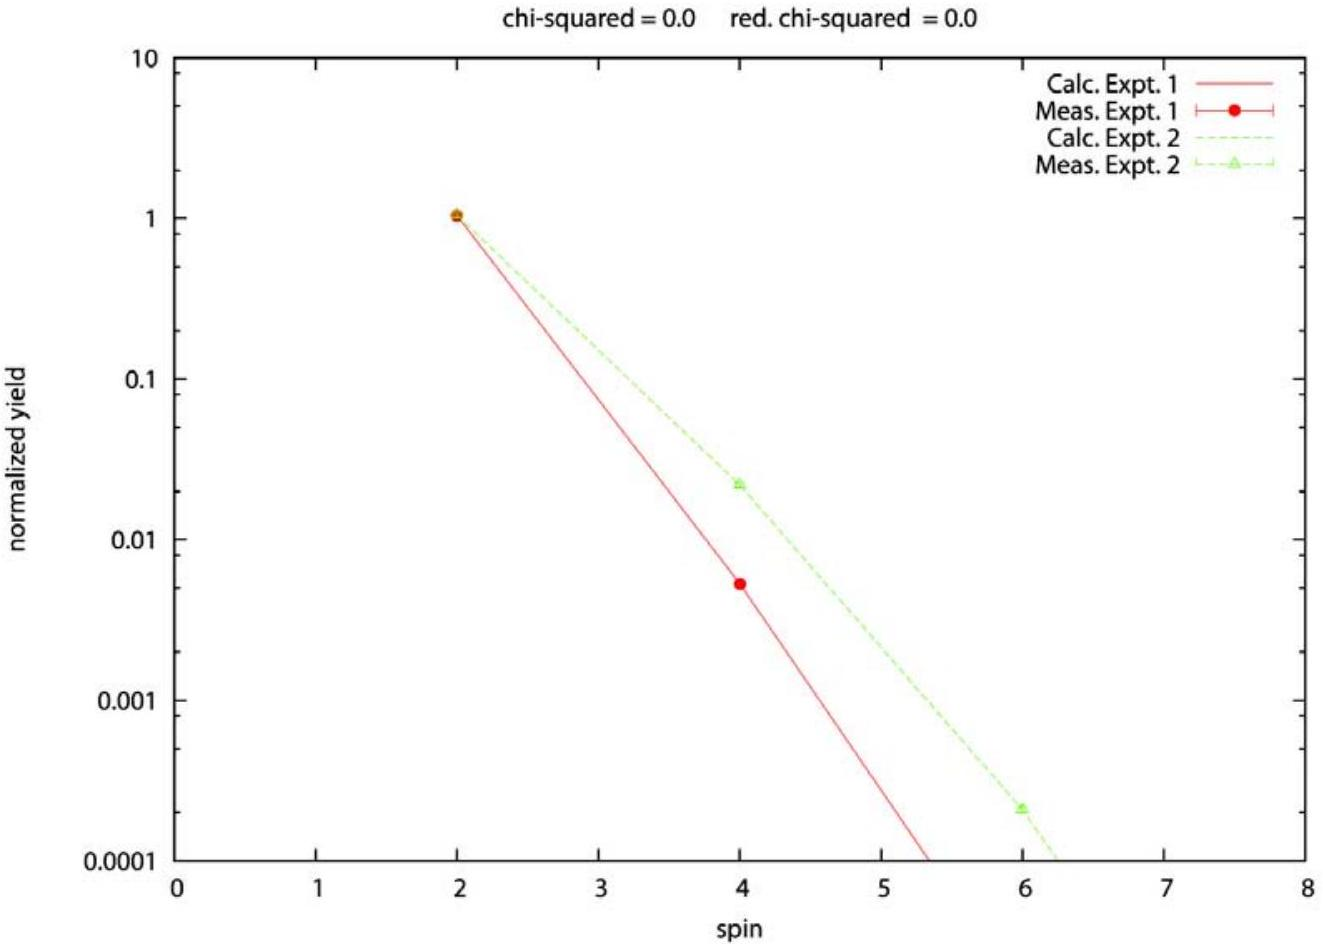
\includegraphics[max width=\textwidth, center]{2025_02_07_204a351db2d7f48b61ebg-274(1)}

Figure 14.10: The measured (simulated) $p-\gamma$ yield data and the predicted yields for the yrast states. Note that without introducing random scatter to the data results in extremely small value for the minimum value of $\chi^{2}$.\\
2. Experiments involving light $(\mathrm{A}<50)$ ions or small forward scattering angles may also require setting IS $=1000$ in the INT control. Refer to Chapter 2 regarding the Sommerfeld parameter and the semiclassical approximation.\\
3. In general, using an excessive number of meshpoints in the OP,INTI step may cause convergence problems if the spline interpolation option is not used. Refer to section CONT in the manual regarding the spline option switch. The following are useful starting points for choosing integration meshpoints:\\
a. beam energy meshpoints spaced at approximately 0.5 MeV intervals\\
b. scattering angle meshpoints spaced at approximately 5 degrees\\
c. at least 50 subdivisions in energy and scattering angle

Meshpoints will need to be spaced more closely for far forward scattering.\\
4. Using unequal intervals between meshpoints without turning on the spline interpolation option may cause divergence of the integration.

The RACHEL interface selects an appropriate spacing of meshpoints and subdivisions to ensure accuracy in most cases. It can also perform an optional test to evaluate the accuracy obtained with a given mesh. When running GOSIA without the interface, it is a good idea to halve or double the mesh spacing to test for convergence.

Accuracy problems that directly affect the minimization (fitting) could cause a failure to converge at a chisquared minimum (although this is not the only possible cause) or termination of the fit at a false minimum. The accuracy of the minimum can be tested by comparing the experimental data to the integrated yields at the minimum.

\subsection*{14.5 Troubleshooting GOSIA inputs}
When making changes to the input, the following guidelines will help the user avoid introducing inconsistencies. Refer to the relevant sections of the manual for details on the input format. The RACHEL interface makes consistent changes to the input within its capabilities (Chapter 8).

\begin{itemize}
  \item When the level scheme (LEVE) or matrix elements (ME) are changed, the following items should be checked. The transition energies and multipolarities defined in LEVE and ME require internal conversion coefficients in OP,YIEL which cover the range of transition energies for each multipolarity introduced in ME. Note that the level energies are entered in MeV, not keV. OP,BRIC is recommended, so that these quantities will be updated automatically.
  \item Changes that affect the kinematics (projectile or target species, beam energy, target thickness, scattering angle ranges, etc.) should be checked for consistency in the EXPT, OP,YIEL and OP,INTI sections. If OP,INTG must be used (generally only when only one kinematic solution is detected and the relevant logical experiment needs to be normalized to another) pay special attention to the selection of the detected particle and whether the projectile scattering or target recoil angles are being specified in each section, as well as the accompanying kinematic flags (minus signs). (The present version of RACHEL uses OP,INTI rather than OP,INTG.) Target thickness is specified indirectly through a range of beam energy and stopping power data. Stopping powers may need to be updated when the beam energy range is changed, or when the beam or target species is modified.
  \item If one experiment (EXPT) is normalized to another, relative particle-detector normalization constants must be entered in OP,YIEL. Inaccuracies in these normalizations will not affect the yield integration (OP,INTI) or correction factors (OP,CORR), but they will cause problems in finding the true chisquared minimum (OP,MINI). Refer to the manual entry for OP,YIEL to find the correct definition of these constants.
\end{itemize}

The safest approach to avoid introducing errors is to make changes to the input in the smallest possible increments, running the code frequently to check for problems. The following troubleshooting notes may be helpful.

\begin{itemize}
  \item Pay special attention to commas and periods; interchanging one for the other is a common cause of errors that are difficult to spot. The RACHEL interface generates (and runs) GOSIA inputs that are free of this type of mistake.
  \item Check the auxiliary files created by GOSIA. Occasionally, an overflow will result in "INF" (infinity) or "NaN" ("Not a Number") being written into a file such as TAPE 4 (the correction factor file). This may cause problems later, when GOSIA re-reads the file. Problems with the corrected yields usually result in an endless loop in the minimization (OP,MINI), with "expansion failures" reported in the output file.
  \item GOSIA will tolerate comments on some lines in the input (after the required fields), but not on others. Putting comments on the wrong line could cause read errors. When in doubt, do not insert a comment.
  \item If an error occurs when GOSIA reads the input file, it may be helpful to insert OP,EXIT (to halt execution) immediately before another "OP," command in the input and run it again to determine which section contains the problem. Do not insert OP,EXIT within the data for the preceding OP,XXXX command; always insert it after all of the required data.
  \item Many integers that are entered in the input file (and in TAPE 3, experimental gamma-ray yields) determine the number of records and fields to follow, or the number of corresponding records in a later section. Errors are frequently caused by inconsistencies in these numbers and may be indicated by messages such as "UNRECOGNIZED SUBOPTION," or Fortran read errors. If errors are suspected to be caused by a mismatch in the number of records and cannot be found by a cursory inspection, it is often helpful to check each line of the input, comparing it to the corresponding manual entry.
\end{itemize}

The following is an example of the above type of error. The execution terminates with this error:\\
invalid integer: read unexpected character\\
apparent state: unit 5 (unnamed)\\
last format: list io\\
lately reading sequential formatted external I\\
Abort\\
This is a Fortran (system) error that is not trapped by GOSIA, so the location of the problem is not specified. Running the input again with OP,EXIT inserted immediately after OP,YIEL to halt the execution results in the same error, but inserting OP,EXIT just before OP,YIEL prevents the error. Hence, the error is somehow related to OP,YIEL. The beginning of OP,YIEL looks like this:

\begin{verbatim}
OP,YIEL
O
18,1
0.056,0.068,0.082,0.1,0.12,0.15,0.18,0.22,0.26,0.32,0.38,
0.46,0.56,0.68,0.82,1.0,1.2,1.5
2
41.7,17.6,7.97,3.58,1.78,0.785,0.415,0.212,0.124,0.0660,0.04,
    0.0241,0.0148,0.00939,0.00623,0.00413,0.00288,0.00188
1,1
1
4 5
90
\end{verbatim}

The EXPT section defines 3 experiments:

\begin{verbatim}
EXPT
3,72,178
54,136,642,24.0,4,0,0,0,360,1,1
54,136,642,42.0,4,0,0,0,360,1,1
54,136,642,60.0,4,0,0,0,360,1,1
\end{verbatim}

However, line 8 in OP,YIEL " 1,1 " contains only 2 values of NANG(I), but the entry for NANG(I) In section\\
7.32 of this manual states that NANG(I) needs to be entered once for each experiment. Line 8 needs to be corrected; in this case a third value should be added to specify the number of gamma-ray detectors for the third experiment. The rest of OP,YIEL should be checked for similar omissions. Stubborn errors can be found most efficiently by checking line-by-line against the required format in the manual.

\section*{Chapter 15}
\section*{$\gamma$-ray detection efficiency: GREMLIN }
The FORTRAN program GREMLIN ("Gamma-Ray Efficiency Measurement and Line INtensity calculation") was developed at Rochester in 1987 by Alexander Kavka. The purpose is to simplify the routine procedure of $\gamma$-ray detector efficiency calibration and detection efficiency correction of measured peak areas for deexcitation $\gamma$-ray yields following Coulomb excitation.\\
GREMLIN can perform two separate tasks:

\begin{enumerate}
  \item Least-squares fit of a $\gamma$-ray detection efficiency-calibration function to a set of peak areas from $\gamma$-ray calibration spectra.
  \item Calculation of detection-efficiency corrected $\gamma$-ray intensities from peak areas, using the fitted efficiency function for the Doppler shift corrected $\gamma$-ray energy.
\end{enumerate}

The functional form of the dependence of detection efficiency on $\gamma$-ray energy is factored into terms that separately account for $\gamma$-ray absorption, high and low energy dependence, and electronic thresholds in order to obtain well-behaved functions that do not exhibit pathological behaviour such as at $K$-edges.

GREMLIN is an essential component of the GOSIA suite of Coulomb excitation analysis codes and can be used in either of two modes. One approach is to use GREMLIN to correct the raw peak areas of the observed deexcitation $\gamma$-rays to account for the $\gamma$-ray detector efficiency at the appropriate Doppler-shifted energy. These corrected yields then are input as the data to be fit by GOSIA. The second approach is to use the GOSIA option OP,RAW which allows input to GOSIA of the raw, i.e. not detector efficiency corrected, $\gamma$-ray yields. The parameters for the $\gamma$-ray detection efficiency function, as determined by the GREMLIN least-squares fit, are used by OP,RAW to detector-efficiency correct the raw yields input to GOSIA.

The code GREMLIN is interactive, and its prompts and questions are hopefully sufficient to guide the user. Therefore, this memo provides no real input instructions, with one exception: it describes the structure of the input files containing the calibration points.

\subsection*{15.1 Option 1: Efficiency calibration}
\subsection*{1.1 Input of calibration points}
A maximum of 500 calibration points can be entered, grouped in up to 9 independently normalized data sets. Typically, these will originate from runs with different calibration sources, but there can just as well be several sets from the same source. If there is more than one data set, the code will automatically fit normalization parameters.

GREMLIN will ask for calibration points for each data set separately. For each set the input can be from a disk file or from the keyboard, and consists of one record for each calibration line. A record looks as follows:

$$
E, \quad I, \quad \Delta I, \quad A, \quad \Delta A
$$

where $E$ is the $\gamma$-ray energy, $I \pm \Delta I$ the tabulated relative intensity, and $A \pm \Delta A$ the measured peak area. Note that two data sets cannot be in one file.

However, the input is simplified in the case of ${ }^{152} \mathrm{Eu}$ or ${ }^{182} \mathrm{Ta}$ sources, because the energies and intensities of major ${ }^{152} \mathrm{Eu}$ and ${ }^{182} \mathrm{Ta}$ transitions are stored in DATA statements in the program. These values were taken from R.A. Meyer: Multigamma-Ray Calibration Sources (Lawrence Livermore Laboratory 1978). The record format is then

$$
A, \quad \Delta A
$$

If keyboard input was chosen, the code will display each tabulated energy and intensity and ask for the area and error. In an input file, the ${ }^{152} \mathrm{Eu}$ or ${ }^{182} \mathrm{Ta}$ lines must be given according to the following table:

\begin{center}
\begin{tabular}{|c|c|c|}
\hline
\begin{tabular}{c}
line \\
number \\
\end{tabular} & \begin{tabular}{c}
152 Eu \\
$(\mathrm{keV})$ \\
\end{tabular} & \begin{tabular}{c}
182 Ta \\
$(\mathrm{keV})$ \\
\end{tabular} \\
\hline
1 & 121.783 & 31.737 \\
2 & 244.692 & 65.722 \\
3 & 295.939 & 67.750 \\
4 & 344.276 & 84.680 \\
5 & 367.789 & 100.106 \\
6 & 411.115 & 113.673 \\
7 & 443.967 & 116.421 \\
8 & 488.661 & 152.430 \\
9 & 564.021 & 156.390 \\
10 & 586.294 & 179.397 \\
11 & 688.678 & 198.350 \\
12 & 778.903 & 222.108 \\
13 & 867.388 & 229.322 \\
14 & 964.131 & 264.078 \\
15 & 1005.279 & 927.983 \\
16 & 1085.914 & 1001.696 \\
17 & 1112.116 & 1113.414 \\
18 & 1212.950 & 1121.299 \\
19 & 1299.124 & 1157.505 \\
20 & 1408.011 & 1189.051 \\
21 & 1528.115 & 1221.406 \\
22 &  & 1231.019 \\
23 &  & 1257.421 \\
24 &  & 1273.735 \\
25 &  & 1289.158 \\
\hline
\end{tabular}
\end{center}

Any unobserved line that is to be excluded from the fit must be entered as $A=\Delta A=0$, at the keyboard as well as in a file. Data for other sources than ${ }^{152} \mathrm{Eu}$ and ${ }^{182} \mathrm{Ta}$ easily can be added to the code in the future, should the need arise. Similarly it is trivial to include additional ${ }^{152} \mathrm{Eu}$ and ${ }^{182} \mathrm{Ta}$ lines in the lists.

\subsection*{1.2 Experimental and theoretical efficiency}
For each calibration line GREMLIN calculates the relative efficiency and root-mean-square error:

$$
\varepsilon=\frac{A}{I} \quad \Delta \varepsilon=\varepsilon \sqrt{\left(\frac{\Delta A}{A}\right)^{2}+\left(\frac{\Delta I}{I}\right)^{2}}
$$

and makes a transformation to the variables which are then internally used for the fit, i.e.

$$
x \equiv \log \frac{E}{E_{0}} \quad y \equiv \log \varepsilon \quad \Delta y=\frac{\Delta \varepsilon}{\varepsilon}
$$

The logarithms are of base $e$ and $E_{0}=50 \mathrm{keV}$.\\
The functional form used by GREMLIN is factored into four functions that separately account for $\gamma$-ray absorption, higher energy, lower energy detection efficiencies, and electronic thresholds in order to obtain\\
well-behaved functions that do not exhibit pathological behaviour such as at K-edges etc. That is, the functional form of the detection efficiency used is

$$
\varepsilon(E)=A(E) P\left(E ; a_{1} \ldots a_{n}\right) F(E ; f) W(E ; b, c)
$$

with the parameters $a_{1} \ldots a_{n}, f, b$, and $c$ to be determined. The separate terms are discussed below.

\subsection*{1.3 Attenuation factor}
$$
A(E)=\exp \left[-\sum_{i=1}^{m} \mu_{i}(E) d_{i}\right]
$$

$A(E)$ stands for the absorption in layers of $m$ different materials placed in front of the detector, $\mu_{i}$ and $d_{i}$ being the linear attenuation coefficient and the thickness of the $i$ th material, respectively.

The absorber materials that GREMLIN takes into account are $\mathrm{C}, \mathrm{Al}, \mathrm{Si}, \mathrm{Fe}, \mathrm{Cu}, \mathrm{Cd}, \mathrm{Sn}, \mathrm{Ta}$, and Pb . The thicknesses (in cm ) are given by the user from the keyboard. DATA statements in the code contain the attenuation coefficient of each material for 20 gamma energies ranging from 30 to 4000 keV . Interpolation is done by means of cubic spline curves. Two of the energy meshpoints were chosen to be 67.416 and 88.004 kev, which are the K-edges of Ta and Pb respectively, and for each of those elements GREMLIN maintains two spline curves, below and above the edge. All other absorption edges for these nine elements lie below 30 keV.

The variables actually used for the spline curves are $\log \frac{E}{E_{0}}$ and $\log \frac{\mu}{m u_{0}}\left(\mu_{0}=1 \mathrm{~cm}^{-1}\right)$, since the points are more evenly spaced in the log-log plane.

The attenuation coeffcients were calculated from total cross-sections $\sigma$ given in E. Storm, H. I. Israel, Nuclear Data Tables A7 (1970) 565, according to

$$
\mu\left[\mathrm{cm}^{-1}\right]=\frac{\rho N_{A} \sigma}{M}=0.602205 \frac{\rho\left[\mathrm{~g} / \mathrm{cm}^{3}\right] \sigma[\mathrm{barn}]}{M[\mathrm{~g} / \mathrm{mol}]}
$$

where $\rho$ is the density, $N_{A}$ Avogadro's number, and $M$ the atomic weight.

\subsection*{1.4 Polynomial factor}
The polynomial factor, degree $n \leq 3$,

$$
P\left(E ; a_{1} \ldots a_{n}\right)=\exp \left[\sum_{k=0}^{n} a_{k}\left(\log \frac{E}{E_{0}}\right)^{k}\right]
$$

is a simple representation of the basic decrease of the efficiency with increasing $\gamma$ energy. The word "polynomial" refers, of course, to $\log \epsilon$ as function of $\log E$.

The degree $n$ is chosen by the user. GREMLIN finds good initial values for the parameters $\alpha_{\kappa}$ by fitting a pure $n$ th-degree polynomial in the region above 250 keV , where $P(E)$ can be expected to dominate.

\subsection*{1.5 Functions describing the low-energy slope}
An inverse-power factor, with arbitrary $N>0$, and $f<0$,

$$
F\left(E ; a_{1} \ldots a_{n}\right)=\exp \left[f\left(\log \frac{E}{E_{0}}\right)^{-N}\right]
$$

and a "Woods-Saxon"-type factor, with $b$ and $c>0$,

$$
W(E ; b, c,)=\frac{1}{1+\exp \frac{b-E}{c}}
$$

are optional, and are unlikely to be used simultaneously, although the code allows that both be used simultaneously. Each represents the low-energy slope of the efficiency curve. Whereas $F$ is just an ad hoc\\
mathematical function, $W$ attempts to model the effect of a discriminator threshold in the pulse-handling electronics.

When $F$ was used, good results were obtained with e.g. $N=5$, but the value of $N$ does not seem to very crucial. An initial value for the parameter $f$ is found by simply sampling the value of $x^{2}$ throughout a range of $f$. The range and stepsize are given by the user, but if the code finds the optimum value at an endpoint of the range, it requests a new range and tries again.

Initial values (in keV) for the parameters $b$ and $c$, in the "Woods-Saxon" case, are given by the user. They are easy to estimate, $b$ being the threshold and $c$ a measure of the "rise time" of this step function.

\subsection*{1.6 Normalization between data sets}
In case of more than one data set, initial normalization factors are chosen in the following way: A linear function

$$
y^{(j)}=a_{0}^{(j)}+a_{1}^{(j)} x
$$

is fitted to every data set in the region $E>250 \mathrm{keV}$ ( $j$ labels the data sets). The efficiency values in data set $\# j$ are then rescaled by replacing $y$ with $y+a_{0}^{(1)}-a_{0}^{(j)}$. This is done before determining initial values for the other parameters.

During the main fit, each normalization parameter is corrected after every iteration by a simple $\chi^{2}$ scan throughout a range of its value. The scan does not have to be iterated, since there is no correlation between the normalization factors.

\subsection*{1.7 The main fit}
When all parameters have been given starting values, the full function is fitted to the calibration points by an interactive matrix inversion method (the same that is used for peak-shape fitting in SILVIA). After every iteration (and renormalization, in case of more than one data set) the program displays the $\chi^{2}$ and the new parameter values and the user decides whether to continue or stop. Convergence is usually rapid thanks to good initial values - often only 2 or 3 iterations of the main fit are necessary.

When the fit is stopped, GREMLIN reports the best (not necessarily the latest) $\chi^{2}$, the corresponding fitted parameters with errors and correlation matrix and a table showing values of th fited fuction in comparison with the measure efficiencies. Three optional output files can be written on disk at this moment:

\begin{enumerate}
  \item A text file showing the results of the fit in the same way as on the screen.
  \item An input file for TOPDRAWER that can generate a log-log plot of the calibration points and the fitted curve on the laser printer. The user can specify a header text and a different point plot symbols for each data set.
  \item A storage file containing the fitted parameter values, information about the functional form used, and absorber thickneses. This file is read by GREMLIN's Option 2 to calculate $\gamma$-ray intensities.
\end{enumerate}

\subsection*{15.2 Option 2: Intensity calculation}
In this option, the program reads a storage file written by Option 1, and then can re-create the fitted function $\varepsilon(E)$. It also asks the user to specify the kinematics of the experiment (masses of projectile and target; bombarding energy; mass and direction $\theta, \phi$ of radiating ejectile) as well as the angular position $\theta_{\gamma}, \phi_{\gamma}$ of the $\gamma$ detector, so that the efficiencies can be calculated for the actually detected (Doppler-shifted) $\gamma$ energies.

The shifted energy is

$$
E^{\prime}=\frac{E}{1-\frac{\nu}{c} \cos \alpha}
$$

where the velocity $\nu$ is calculated from the kinematics and $\alpha$ is the angle between the $\gamma$-ray and the radiating nucleus.

$$
\cos \alpha=\sin \theta \sin \theta_{\gamma} \cos \left(\phi-\phi_{\gamma}\right)+\cos \theta \cos \theta_{\gamma}
$$

The user now types a series of transition energies $E$ and peak areas $A \pm \Delta A$, and GREMLIN returns the corresponding relative intensities

$$
I=\frac{A}{\varepsilon\left(E^{\prime}\right)}
$$

and errors $\Delta I$. The errors are calculated from

$$
\left(\frac{\Delta I}{I}\right)^{2}=\left(\frac{\Delta A}{A}\right)^{2}+\left(\frac{\Delta \varepsilon}{\varepsilon}\right)^{2}
$$

where the efficiency error is estimated using the correlation matrix $C$ that results from the fit:

$$
(\Delta \varepsilon)^{2}=\sum_{j=1}^{p} \sum_{k=1}^{p} \frac{\partial \varepsilon}{\partial \alpha_{j}} \frac{\partial \varepsilon}{\partial \alpha_{k}} C_{i j}
$$

$a_{j}(j=1 \ldots p)$ represents all the parameters of the fit.\\
The derivatives with respect to the parameters have simple analytical expressions:

$$
\begin{array}{cc}
\frac{\partial \varepsilon}{\partial \alpha_{j}}=\varepsilon\left(E^{\prime}\left(\log \frac{E^{\prime}}{E_{0}}\right)^{j}\right. & \frac{\partial \varepsilon}{\partial f}=\varepsilon\left(E^{\prime}\right)\left(\log \frac{E^{\prime}}{E_{0}}\right)^{-N} \\
\frac{\partial \varepsilon}{\partial b}=-\frac{\varepsilon\left(E^{\prime}\right)}{c\left(1+\exp \frac{E^{\prime}-b}{c}\right)} & \frac{\partial \varepsilon}{\partial c}=\frac{E^{\prime}-b}{c} \frac{\partial \varepsilon}{\partial b}
\end{array}
$$

\section*{Chapter 16}
\section*{Release notes}


\subsection*{16.1 General}
The original GOSIA code was developed in 1980 by T. Czosnyka, D. Cline and C.Y. Wu at the University of Rochester. In the years since, several other versions of the code have been developed: GOSIA2 and PAWEL by T. Czosnyka, ANNL by R. Ibbotson, while the GOSIA graphical user interface RACHEL was developed by A. Hayes. These Release notes include updates as of 8 June 2011. These release notes do not necessarily apply to PAWEL or ANNL.

The coding of the GOSIA suite of codes was maintained by Tomasz Czosnyka from 1980 until his untimely death in 2006. Since 2007 Nigel Warr has upgraded the coding of GOSIA and GOSIA2 in conjunction with the other members of the Gosia Steering Committee while the testing has been performed by Adam Hayes. Responsibility for the management and development of the Gosia suite of codes was assumed by the Steering Committee of the Gosia Users Group in April 2008.

The Gosia Steering Committee comprises:\\
Douglas Cline (University of Rochester)\\
Adam Hayes (University of Rochester)\\
Pawel Napiorkowski (Warsaw University)\\
Nigel Warr (University of Cologne)\\
Valuable contributions to the development of GOSIA were made by L. Hasselgren (Uppsala), R. Ibbotson (Rochester), A.E. Kavka (Uppsala and Rochester), B. Kotlinski (Warsaw and Rochester), J. Srebrny (Warsaw), Eh. Vogt (München and Rochester)

\subsection*{16.2 References and Credits}
T. Czosnyka, D. Cline and C. Y. Wu, Bull. Am. Phys. Soc. 28, 745 (1983).

University of Rochester internal laboratory report UR/NSRL 308/1986\\
Some concepts used were taken from the 1978 Winther, de Boer code COULEX and from the deexcitation code CEGRY developed by Cline and coworkers at Rochester. However, the parts taken from both codes are in most cases completely rewritten, so the similarity of variable and routine names may be misleading.

\subsection*{16.3 Compiling GOSIA}
GOSIA compiles on most 64 -bit systems with GNU g77, using the default compiler settings. Previous versions of the Gosia code did not explicitly specify 64 -bit precision and were intended to be compiled by the user at the highest machine precision available. The current availability of 64 -bit machines and the accuracy problems which may arise when relying on 32 -bit precision led to the decision to make this code explicitly 64 -bit. Modifying the code to run with 32 -bit precision is strongly discouraged.

\subsection*{16.4 Recent upgrades}
The Gosia 2012 suite of codes include significant upgrades both to the functionality and to the coding compared with the last versions developed by Tomasz Czosnyka in 2006.

\section*{Functionality upgrades:}
The following have been implemented in both the Gosia and Gosia2 codes.

\begin{enumerate}
  \item Dimensions:
\end{enumerate}

The number of levels has increased from 75 to 99 while the total number of magnetic substates has been increased from 600 to 1200 . The number of electromagnetic matrix elements has increased from 500 to 999. These changes are to accommodate the larger dimension systems encountered in analysis of Coulomb excitation measurements performed using the high-sensitivity new generation detector arrays.\\
2) Internal conversion coefficients:

The BrIcc internal conversion coefficient database supported by the National Nuclear Data Center has been incorporated in Gosia. This allows direct calculation of the internal conversion coefficients for every transition included in the input significantly reducing the amount of data that needs to be typed into the Gosia input file.\\
3) Spline interpolation:

A spline interpolation procedure has been implemented to eliminate the persistent problem of wild oscillatory behaviour that occurs when many meshpoints are used with Lagrange interpolation. The cubic spline subroutines SPLINE and SPLINT were taken from "Numerical Recipes in Fortran" [PRE92].\\
4) Energy and angle meshpoints:

The number of energy and angle meshpoints used in integration have each been increased to 100 to improve the accuracy. This upgrade was made possible by changing from Lagrange to spline interpolation.\\
5) Error correlation matrix:

The generation of the error correlation matrix has been incorporated in a new OP,SELE (SELECT) routine eliminating the need to run the external program SELECT.\\
6) Inverse kinematics:

The handling of inverse kinematics has been improved to eliminate problems due to two-valued solutions for projectile scattering angles and the peaked Jacobian at the maximum scattering angle of the scattered projectile. The integration over target-recoil angle is done in the laboratory frame.\\
7) Physical constants:

More accurate physical constants have been used to evaluate constants incorporated in Gosia.\\
8) Graphical user interface:

Adam Hayes developed a graphical user interface, called RACHEL, that automates generation of the complicated input required to use GOSIA. This greatly simplifies use of GOSIA as well as incorporating additional features such a generation of simulated data with realistic errors for planning experiments.

\section*{Coding upgrades:}
Nigel Warr has implemented the following improvements to the underlying Fortran coding to eliminate bugs and produce more reliable executables.

\begin{enumerate}
  \item Explicit 64-bit Precision Upgrade:
\end{enumerate}

Previous versions of the GOSIA code did not explicitly specify 64-bit precision; the user was expected to compile the code at the highest machine precision available. The current availability of 64 -bit machines and the accuracy problems which arise when relying on 32-bit precision led to the decision to make the 2007 version fully and explicitly 64 -bit. Modifying the code to run with 32 -bit precision is discouraged. Earlier versions of GOSIA had some portability problems arising from misalignment of common blocks. In GOSIA 2007 the common blocks have been re-ordered so that the 64 -bit real variables come before the 32-bit integer variables, in order to eliminate alignment problems.\\
2) Structure and standards:

The 2007 code has been updated to replace many archaic Fortran functions with their modern counterparts. Sections of the code have been restructured using SPAG (C Polyhedron Software) under the academic license. This included unraveling of loops and goto statements, reordering variables so that declarations and common blocks are together, and indenting the source code to make loops and if statements more obvious. The initialization in the main routine has been slightly restructured, mainly to make it similar to the 2007\\
version of GOSIA2. Other sections have been restructured and commented for clarity, without altering their function.\\
3) The physical constants in the code were changed to more accurate values.\\
4) Bugs fixed:

The subroutine in GOSIA which calculates the rotation functions relies on its memory space for local variables being preserved between calls. This occurred automatically on many older systems (e.g. DEC Alpha, VAX). On some newer machines these variables were being lost, causing unpredictable errors, such as negative values of chi-squared. This has been fixed in the 2007 version.

If the user requests an excessive number of Coulomb excitation calculations requiring high accuracy, GOSIA may find that its allocated memory is insufficient for the number of collision functions required (Chapter 3). Previous versions of GOSIA did not terminate execution according to Fortran standards when this occurred, and execution would continue on some newer platforms. This may cause reports of "NaN" in the output file(s), resulting in read errors later. This bug has been fixed. If GOSIA 2007 finds an insufficient memory condition, it reports the error and terminates the job.

The WRN,X. switch in the CONT section of both OP,GOSI and OP,COUL was unintentionally disabled in the 2007 version. It is restored in the present update.

A discontinuity in the TRINT routine was discovered and corrected.\\
For projectile excitation the relativistic transformation from the emitter to laboratory frame was found to be performed in the $-\theta_{\text {projectile }}$ direction rather than the correct $\theta_{\text {projectile }}$ direction. This error was corrected in versions Gosia\_20081208.10.f and Gosia2\_20081208.11.f.\\
5) Input format:

Tapes 1 and 2 in the pre- 2007 versions have been reassigned to tapes 11 and 12 , respectively, in order to make switching between GOSIA and GOSIA2 (the mutual excitation code) easier. This change affects only the default naming of files by GOSIA and the tape 1 and 2 entries to OP,FILE (optional-see below). For example, on a typical Unix-like system, if OP,FILE is not used, the file formerly called "fort.2" will now be called "fort.12" and will contain the best set of matrix elements written at the end of the minimization.

\subsection*{16.5 GOSIA development history}
Nigel Warr maintains a compilation of the current versions of the fortran Gosia files plus the chronology and major changes made to Gosia during the period 2007-2011. These can be found on Nigel Warr's Gosia web site (\href{http://www.ikp.uni-koeln.de/~warr/gosia/}{http://www.ikp.uni-koeln.de/\~{}warr/gosia/}). These previous versions should (in theory) be similar in the way they work, but if you find a bug in the most recent version, please test some of the older versions to help track down where the bug was introduced. The versions have a date stamp YYYYMMDD and possibly a sub-version. Sub-versions are for bugfixes only (relative to the major version with the date stamp).The chronology and major changes for the Gosia codes are reproduced below.

\subsection*{16.5.1 Chronology of major changes to GOSIA: 2007-2012}
\begin{center}
\begin{tabular}{|c|c|c|}
\hline
Date & File & Comments \\
\hline
7/11/11 & gosia\_20110524.2.f & Bugfix relative to 20110524.1 (Fix bug in $\lambda=6, \mu=3$ collision functions). \\
\hline
10/10/11 & gosia\_20110524.1.f & Bugfix relative to 20110524 (Fix bug causes a failure when a meshpoint in inverse kinematics is at the target angle corresponding to the maximum projectile angle). \\
\hline
24/5/11 & gosia\_20110524.f & Version including extra options for Rachel \\
\hline
7/11/11 & gosia\_20081208.12.f & Bugfix relative to 20081208.11 (Fix bug in $\lambda=6 \mu=3$ collision functions). \\
\hline
10/10/11 & gosia\_20081208.11.f & Bugfix relative to 20081208.10 (Fix bug causes a failure when a meshpoint in inverse kinematics is at the target angle corresponding to the maximum projectile angle). \\
\hline
24/6/10 & gosia\_20081208.10.f & Bugfix relative to 20081208.9 (Fix bug in relativistic correction for inverse kinematics). \\
\hline
22/2/10 & gosia\_20081208.9.f & Bugfix relative to 20081208.8 (Fix discontinuity in TRINT). \\
\hline
18/9/09 & gosia\_20081208.8.f & Correction to 20081208.7 \\
\hline
14/9/09 & gosia\_20081208.7.f & Improve 20081208.6 (Increased dimensions in ZETA to allow 999 matrix elements). \\
\hline
16/8/09 & gosia\_20081208.6.f & Bugfix relative to 20081208.5 (Increased dimensions in VLIN to 101). \\
\hline
20/7/09 & gosia\_20081208.5.f & Bugfix relative to 20081208.4 (integration over PIN diodes was incorrect). \\
\hline
2/4/09 & gosia\_20081208.4.f & Bugfix relative to 20081208.3 (E1 polarization was incorrect). \\
\hline
1/2/09 & gosia\_20081208.3.f & Bugfix relative to 20081208.2 (OP,INTI preserves IKIN flag). \\
\hline
27/1/09 & gosia\_20081208.2.f & Bugfix relative to 20081208.1 (OP,INTI got wrong particle for target excitations). \\
\hline
16/1/09 & gosia\_20081208.1.f & Bugfix relative to 20081208 (give error if too many omega steps). \\
\hline
8/12/08 & gosia\_20081208.f & New OP,INTI option for inverse kinematics (beta version) - see doc here. \\
\hline
24/6/10 & gosia\_20080630.7.f & Bugfix relative to 20080630.7 (Fix bug in relativistic correction for inverse kinematics). \\
\hline
22/2/10 & gosia\_20080630.7.f & Bugfix relative to 20080630.6 (Fix discontinuity in TRINT). \\
\hline
18/9/09 & gosia\_20080630.6.f & Correct 20080630.5 \\
\hline
14/9/09 & gosia\_20080630.5.f & Improve 20080630.4 (Increased dimensions in ZETA to allow 999 matrix elements). \\
\hline
16/8/09 & gosia\_20080630.4.f & Bugfix relative to 20080630.3 (Increased dimensions in VLIN to 101). \\
\hline
20/7/09 & gosia\_20080630.3.f & Bugfix relative to 20080630.2 (integration over PIN diodes was incorrect). \\
\hline
2/4/09 & gosia\_20080630.2.f & Bugfix relative to 20080630.1 (E1 polarization was incorrect). \\
\hline
16/1/09 & gosia\_20080630.1.f & Bugfix relative to 20080630 (Bricc files opened 'OLD'). \\
\hline
30/6/08 & gosia\_20080630.1.f & Up to 99 levels, bugfixes, Radware efficiency calibration. \\
\hline
24/6/10 & gosia\_20080519.10.f & Bugfix relative to 20080519.9 (Fix bug in relativistic correction for inverse kinematics). \\
\hline
22/2/10 & gosia\_20080519.9.f & Bugfix relative to 20080519.8 (Fix dimensions in VLIN). \\
\hline
22/2/10 & gosia\_20080519.8.f & Bugfix relative to 20080519.7 (Fix discontinuity in TRINT). \\
\hline
18/9/09 & gosia\_20080519.7.f & Correct 20080519.6 \\
\hline
14/9/09 & gosia\_20080519.6.f & Improve 20080519.5 (Increased dimensions in ZETA to allow 999 matrix elements). \\
\hline
16/8/09 & gosia\_20080519.5.f & Bugfix relative to 20080519.4 (Increased dimensions in VLIN to 101). \\
\hline
20/7/09 & gosia\_20080519.4.f & Bugfix relative to 20080519.3 (integration over PIN diodes was incorrect). \\
\hline
2/4/09 & gosia\_20080519.3.f & Bugfix relative to 20080519.2 (E1 polarization was incorrect). \\
\hline
16/1/09 & gosia\_20080519.2.f & Bugfix relative to 20080519.1 (give error if too many omega steps). \\
\hline
19/5/08 & gosia\_20080519.f & Bugfix relative to 20080519 (several small bugs). \\
\hline
19/5/08 & gosia\_20080519.f & Spline, Bricc option for conversion coefficients, OP,SELE. \\
\hline
8/5/08 & gosia\_20080508.f & Up to 999 matrix elements. \\
\hline
7/5/08 & gosia\_20080507.f & Corrected constants. \\
\hline
18/4/08 & gosia\_20080418.f & Allow up to 50 meshpoints in energy and theta, Leuven efficiency calibration. \\
\hline
28/3/08 & gosia\_20080328.f & Minor bugfix. \\
\hline
29/2/08 & gosia\_20080229.f & Warn user if NI2 exceeds 50. \\
\hline
26/7/07 & gosia\_20070726.f & Cleanup of code. \\
\hline
21/7/07 & gosia\_20070721.f & Small bugfixes. \\
\hline
17/7/07 & gosia\_20070717.f & Small bugfixes. \\
\hline
9/7/07 & gosia\_20070709.f & 64 -bit version. \\
\hline
June/06 & gosia\_06.f & 32 bit. Needs special compiler options (e.g. -fno-automatic for g77). \\
\hline
\end{tabular}
\end{center}

\subsection*{16.5.2 Change log for GOSIA: 2007-2012}
\section*{20110524}
\begin{itemize}
  \item Adam Hayes's modifications for Rachel
\end{itemize}

\subsection*{20081208.10.a}
An extended Gosia version based on release 20081208.10, called 20081208.10.a, makes use of the previously unassigned PRT (printout) option 9 and the previously unused output file number 99 to generate output of the Coulomb excitation amplitudes and collision functions, both as a function of time. This extended version is meant for use with the Rachel GUI, which can plot the amplitude and collision functions as diagnostic tools.

\subsection*{20081208.10}
\begin{itemize}
  \item New option OP,INTI which works like OP,INTG but the theta values for the meshpoints are given as labortatory angles for the detected particle which can be the recoiling target nuclei in the laboratory frame. This helps inverse kinematics cases where only the recoiling target nucleus is detected.\\
${ }^{\circ}$ Fixed bug in relativistic correction for inverse kinematics
\end{itemize}

\section*{20080630.8}
\begin{itemize}
  \item Reordering of all variable declarations so variables in common blocks are together.
  \item Increased size of arrays fro levels from 75 to 99.\\
${ }^{\circ}$ Change in many format statements to accommodate 99 levels (I2 -> I3).\\
${ }^{\circ}$ Increased size of arrays for substates from 600 to 1200.\\
${ }^{\circ}$ Restructure function EFFIX to allow more flexible selection of efficiency calibration type.
  \item Added Radware efficiency calibration (Pawel J. Napiorkowski).
  \item Added EFF, option to CONT to make it easier to select efficiency method.\\
${ }^{\circ}$ Bugfix in gremlin efficiency method: a sign was wrong in Woods-Saxon term.
  \item Bugfix in initialisation of conversion coefficients for interpolation method (only part of array was initialized).\\
${ }^{\circ}$ Add CONTINUE statements to prevent GOTO the ENDDO of a loop. This is deprecated and will be removed in future.\\
${ }^{\circ}$ Call either LAGRAN or SPLNER to do interpolation according to ISPL variable.\\
${ }^{\circ}$ Approximation in TRINT if Arg is very large (then ratio is one) as in Pawel.\\
${ }^{\circ}$ Replaced OPEN(NAME=xxx) with OPEN(FILE=xxx) as the former is an extension to the language, while the latter is standard.\\
${ }^{\circ}$ Bugfix in BRICC: we need the absolute value of the difference in energy levels not the signed difference.\\
${ }^{\circ}$ Use JZB to indicate which unit to read from as in gosia2.\\
${ }^{\circ}$ Use IUNIT3 to indicate which unit is TAPE3 as in gosia2.\\
${ }^{\circ}$ Use irix variable to select units 7 and 12 as in gosia2.\\
${ }^{\circ}$ Add dummy variable Op2 to ANGULA as in gosia2.\\
${ }^{\circ}$ In OPENF we refuse to open units 25 and 26 unless reading from unit 5 as in Ggosia2 (however, gosia always reads from unit 5 , so this does nothing).
  \item Bugfix for dimension of bten, which should have been 1600 and was different in different places.
  \item Use DCMPLX instead of CMPLX for portability.
  \item Use DIMAG instead of IMAG for portability.
  \item Reorder DATA statement in NEWCNV for portability.\\
${ }^{\circ}$ Use LAGRAN for interpolation if there are less than three data points even if ISPL $=1$. 20080519
  \item Add spline support (Pawel J. Napiorkowski).\\
${ }^{\circ}$ Add new version of CONV which can lookup internal conversion coefficients from a table, which must have all the necessary energies (no interpolation).\\
${ }^{\circ}$ Add OP,BRIC to use BrIcc database to generate conversion coefficient table for new version of CONV.
\end{itemize}

\section*{20080508}
${ }^{\circ}$ Increased size of arrays for matrix elements from 500 to 1500 . N.B. we are still limited to 999 matrix elements because 1000 is used as a flag.

\begin{itemize}
  \item Added OP,SELE.
\end{itemize}

20080507\\
${ }^{\circ}$ Correct inaccurate constants in SEQ.\\
${ }^{\circ}$ Replaced constant 10 with NLIFT in loop (this was a bug).\\
${ }^{\circ}$ Initialized some variables explicitly to remove compiler warnings.\\
${ }^{\circ}$ Increased AKAVKA dimensions from 8 to 9 to prepare for merge of Pawel Napiorkowski's efficiency code.

\begin{itemize}
  \item Added ISPL variable in CCC common to prepare for merge of Pawel Napiorkowski's spline code and SPL, option in CONT.\\
${ }^{\circ}$ Restructured a repeated IF with the same condition to use IF/THEN.
\end{itemize}

\section*{20080418}
${ }^{\circ}$ Increased dimensions of arrays fiex1, wpi in GOSIA.\\
${ }^{\circ}$ Increased dimensions of XV, YV, ZV, DSG and DSE in GOSIA.\\
${ }^{\circ}$ Moved OP,EXIT code to end of GOSIA (as in gosia2).\\
${ }^{\circ}$ Limited ABS(NI2) rather than NI2 to 50 in GOSIA.\\
${ }^{\circ}$ Fixed call to MIN so both parameters have same precision in GOSIA.\\
${ }^{\circ}$ Remove unused variables $u$ and $v$ in ALLOC.\\
${ }^{\circ}$ Changed format of normalisation coefficients write in CEGRY.\\
${ }^{\circ}$ Changed dimensions of X, Y, w and arh in LAGRAN.\\
${ }^{\circ}$ Changed dimensions of XV, YV, ZV, DSG and DSE in TAPMA.\\
${ }^{\circ}$ Changed dimensions of Wpi in COORD.\\
${ }^{\circ}$ Changed dimensions of XV, YV, ZV, DSG and DSE in COORD.\\
${ }^{\circ}$ Changed dimensions of XV, YV, ZV, DSG and DSE in KONTUR.\\
${ }^{\circ}$ Added Leuven efficiency calibration in EFFIX (as in gosia2).

\section*{20080328}
\begin{itemize}
  \item Put back warnings in CEGRY which was removed by mistake.
  \item Fix typo misspelling "WARNING" in CEGRY.
\end{itemize}

\section*{20080229}
${ }^{\circ}$ Limit NI2 to 50 in GOSIA.

\section*{20070726}
${ }^{\circ}$ Reorder initialisation so it is similar to gosia2 in GOSIA.\\
${ }^{\circ}$ Remove ineffective attempt to provoke floating point exception in ALLOC.\\
${ }^{\circ}$ Remove superfluous ELSE in WTHREJ.\\
${ }^{\circ}$ Move some format statements in PRELM.

\section*{20070721}
${ }^{\circ}$ Fix initialisation of CNOR from 1 to 75 not 1 to 50 in GOSIA.\\
${ }^{\circ}$ Make both parameters of SIGN have same precision in FXIS1.

\section*{20070709}
${ }^{\circ}$ Restucture IF statement in GOSIA.\\
${ }^{\circ}$ Add explicit STOP statement to ALLOC.

\begin{itemize}
  \item Move duplicated lines out of IF/ELSE in MINI.
  \item Make both parameters of SIGN have same precision in FXIS2.\\
${ }^{\circ}$ Run spag.\\
${ }^{\circ}$ Convert to double precision.
  \item Reorder common LCZP.
  \item Reorder common CAUX0.\\
${ }^{\circ}$ Reorder common COEX.
  \item Reorder common KIN.
  \item Reorder common CCC.\\
${ }^{\circ}$ Reorder common ME2D.\\
${ }^{\circ}$ Declare all variables explicitly.
  \item Add PROGRAM statement to GOSIA.\\
${ }^{\circ}$ Replace ALOG with LOG.
  \item Replace ALOG10 with LOG10.\\
${ }^{\circ}$ Replace AMIN1 with MIN.
  \item Replace MIN0 with MIN.
  \item Replace AMAX1 with MAX.\\
${ }^{\circ}$ Replace MAX0 with MAX.\\
${ }^{\circ}$ Replace IABS with ABS.\\
${ }^{\circ}$ Replace FLOAT with REAL.\\
${ }^{\circ}$ Replace IFIX with INT.
  \item Add SAVE statement in DJMM.
\end{itemize}

\subsection*{16.6 Chronology and change log for GOSIA: 1980-2006}
(June 2006, T. Czosnyka) - The array size for the internal conversion coefficients has been increased to 50. This allows the user to enter more ICC values near discontinuities (i.e., electron binding energies) where several closely spaced values are needed for an accurate interpolation. Refer to OP,YIEL in this manual.\\
(Nov 2000, T. Czosnyka) - A Jaeri efficiency calibration has been added for the Ge detector data.\\
(2000) - A FITEFF Ge efficiency calibration has been added with credit to P. Olbratowski, P. Napiorkowski.\\
(July 1997, T. Czosnyka) - Known matrix elements of all multipolarities may now be entered as data in OP,YIEL. Note that this necessitates adding the multipole order LAMBDA as the first field in the new input format,

LAMBDA, NS1, NS2, ME, DME\\
where LAMBDA $=7$ and 8 represent M1 and M2, respectively.\\
(September 1996, T. Czosnyka) - The PIN diode particle detector option has been added. See the entry for "PIN,X." under the sub-option CONT in this manual.\\
(May 1995, T. Czosnyka) - A collective model matrix element generator "OP,THEO" was added.\\
(April 1991, T. Czosnyka) - The OP,RAW function has been added. OP,RAW handles non-efficiencycorrected gamma-ray yield data and allows the definition of Ge detector "clusters." Up to 20 clusters can be defined. This effectively increases the number of physical Ge detectors to 200 , while the number of data sets (i.e. single detectors + detector clusters) is still limited to 32 .\\
(April 1991, T. Czosnyka) - Output is now written on unit 22 to avoid mixing it with system messages on some systems.\\
(November 1990, T. Czosnyka) - The level scheme data arrays have been increased to the following sizes:

Levels $\quad 75$\\
Gamma-ray yields $32 \times 1500$\\
Magnetic substates 600\\
Matrix elements 500\\
(April 1990, T. Czosnyka) - The dominant multipolarity switch formerly set in the "ME" sub-option (Section 7.16) is now ignored by the code and does not need to be set. Full Q-maps are now calculated for electric multipole orders E1 through E4 (Chapter 2). The electric matrix elements up to multipole order E6 may be entered and fit. The Xi and Zeta function ranges are now calculated for each multipolarity individually (Chapter 3).\\
(1990, Eh. Vogt, T. Czosnyka) - OP,FILE has been added (Section 7.9), giving the user the option of specifying descriptive names of the input and output files in the GOSIA input, rather than using the Fortran default names fort.1, fort.2, etc.\\
(March 1989, T. Czosnyka) - The code has been updated to allow input of gamma-ray yield data from 32 Ge detectors. [As of the 2007 version, this means a total of $32 \times 1500$ data points.]\\
(1980, T. Czosnyka, D. Cline, C.Y. Wu) - Original version.

\subsection*{16.7 GOSIA2 development history}
\subsection*{16.7.1 Chronology of Major Changes to GOSIA2}
Date\\
$7 / 11 / 11$\\
$20 / 5 / 11$\\
20/5/11\\
$24 / 6 / 10$\\
$23 / 4 / 10$\\
$22 / 2 / 10$\\
$14 / 9 / 09$\\
$16 / 8 / 09$\\
$20 / 7 / 09$\\
$2 / 4 / 09$\\
$1 / 2 / 09$\\
$27 / 1 / 09$\\
$23 / 1 / 09$\\
$19 / 1 / 09$\\
$8 / 12 / 08$\\
$24 / 6 / 10$\\
$23 / 4 / 10$\\
$22 / 2 / 10$\\
$14 / 9 / 09$\\
$16 / 8 / 09$\\
$20 / 7 / 09$\\
$2 / 4 / 09$\\
$19 / 1 / 09$\\
$30 / 6 / 08$\\
$30 / 6 / 08$\\
$24 / 6 / 10$\\
$23 / 4 / 10$\\
$22 / 2 / 10$\\
$22 / 2 / 10$\\
$16 / 8 / 09$\\
$20 / 7 / 09$\\
$2 / 4 / 09$\\
$19 / 1 / 09$\\
$19 / 5 / 08$\\
$18 / 4 / 08$\\
$17 / 4 / 08$\\
$14 / 4 / 08$

Comments\\
Bugfix relative to 20081208.13 (Fix bug in lambda $=6 \mathrm{mu}=3$ collision functions)\\
Bugfix relative to 20081208.12 (Fix bug causes a failure when a meshpoint in inverse. kinematics is at the target angle corresponding to the maximum projectile angle)\\
Bugfix relative to 20081208.11 (Fix bug which overwrites files).\\
Bugfix to 20081208.10 (Fix bug in relativistic correction for inverse kinematics).\\
Bugfix relative to 20081208.9 (Fix LCK, control option bug).\\
Bugfix relative to 20081208.8 (Fix TRINT discontinuity bug).\\
Improve 20081208.7 (Increased dimensions in ZETA to allow 999 matrix elements).\\
Bugfix relative to 20081208.6 (Increased dimensions in VLIN to 101).\\
Bugfix relative to 20081208.5 (integration over PIN diodes was incorrect).\\
Bugfix relative to 20080630.8 (Fix bug in relativistic correction for inverse kinematics).\\
Bugfix relative to 20081208.3 (OP,INTI preserves IKIN flag).\\
Bugfix relative to 20081208.2 (OP,INTI got wrong particle for target excitations).\\
Bugfix to 20081208.1 (multiply by dsigma*SIN(theta) for OP,INTI as well as OP,INTG).\\
Bugfix relative to 20081208 (give error if too many omega steps).\\
New OP,INTI option for inverse kinematics (beta version) - see doc here.\\
Bugfix relative to 20080630.8 (Fix bug in relativistic correction for inverse kinematics).\\
Bugfix relative to 20080630.7 (Fix LCK, control option bug).\\
Bugfix relative to 20080630.6 (Fix TRINT discontinuity bug).\\
Improve 20080630.5 (Increased dimensions in ZETA to allow 999 matrix elements).\\
Bugfix relative to 20080630.4 (Increased dimensions in VLIN to 101).\\
Bugfix relative to 20080630.3 (integration over PIN diodes was incorrect).\\
Bugfix relative to 20080630.2 (E1 polarization was incorrect).\\
Bugfix relative to 20080630.1 (give error if too many omega steps).\\
Bugfix relative to 20080630 (Bricc files opened 'OLD').\\
99 levels + 999 matrix elements, Radware efficiency calibration. OP,BRIC is broken\\
Bugfix relative to 20080519.7 (Fix bug in relativistic correction for inverse kinematics).\\
Bugfix relative to 20080519.6 (Fix LCK, control option bug).\\
Bugfix relative to 20080519.5 (Use FILE $=$ not NAME $=$ in open statement).\\
Bugfix relative to 20080519.4 (Fix TRINT discontinuity bug).\\
Bugfix relative to 20080519.3 (Increased dimensions in VLIN to 101).\\
Bugfix relative to 20080519.2 (integration over PIN diodes was incorrect).\\
Bugfix relative to 20080519.1 (E1 polarization was incorrect).\\
Bugfix relative to 20080519 (give error if too many omega steps).\\
Spline, Bricc option for conversion coefficients, OP,SELE, corrected constants Cleanup a bit\\
Allow up to 50 meshpoints in energy and theta, give error if NI2 exceeds 50 .\\
64 -bit version.

\subsection*{16.7.2 Change log for GOSIA2}
20081208.11f (synchronized with gosia1)\\
${ }^{\circ}$ New option OP,INTI which works like OP,INTG but the theta values for the meshpoints are given as angles for the detected particle ( projectile or target) in the\\
laboratory frame. This helps for inverse kinematics cases.\\
20080630.9f (synchronized with gosia1)\\
${ }^{\circ}$ Reordering of all variable declarations so variables in common blocks are together.\\
${ }^{\circ}$ Increased size of arrays for levels from 75 to 100.\\
${ }^{\circ}$ Change in many format statements to accomodate 100 levels (I2 -> I3).\\
${ }^{\circ}$ Increased size of arrays for substates from 600 to 1200.\\
${ }^{\circ}$ Restructure function EFFIX to allow more flexible selection of efficiency calbration type.

\begin{itemize}
  \item Added Radware efficiency calibration (Pawel J. Napiorkowski).\\
${ }^{\circ}$ Added EFF, option to CONT to make it easier to select efficiency method.\\
${ }^{\circ}$ Bugfix in gremlin efficiency method: a sign was wrong in Woods-Saxon term.
  \item Bugfix in initialisation of conversion coefficients for interpolation method (only part of array was initialized).\\
${ }^{\circ}$ Add CONTINUE statements to prevent GOTO the ENDDO of a loop. This is deprecated and will be removed in future.\\
${ }^{\circ}$ Call either LAGRAN or SPLNER to do interpolation according to ISPL variable.\\
${ }^{\circ}$ Approximation in TRINT if Arg is very large (then ratio is one) as in Pawel.\\
${ }^{\circ}$ Replaced OPEN(NAME=xxx) with OPEN(FILE=xxx) as the former is an extension to the language, while the latter is standard.\\
${ }^{\circ}$ Bugfix in BRICC: we need the absolute value of the difference in energy levels not the signed difference.\\
${ }^{\circ}$ Bugfix for dimension of bten, which should have been 1600 and was different in different places.
  \item Use DCMPLX instead of CMPLX for portability.
  \item Use DIMAG instead of IMAG for portability.
  \item Reorder DATA statement in NEWCNV for portability.\\
${ }^{\circ}$ Use LAGRAN for interpolation if less than three data points even if ISPL $=1$\\
20080519 (synchronized with gosia1)\\
${ }^{\circ}$ Add spline support (Pawel J. Napiorkowski)
  \item Add CONT option SPL,
  \item Add OP,SELE
  \item Add OP,BRIC
  \item Add new method of reading conversion coefficients\\
${ }^{\circ}$ Replaced constant 10 with NLIFT in loop (this was a bug)\\
${ }^{\circ}$ Correct inaccurate constants in SEQ
  \item Initialized some variables explicitly to remove compiler warnings\\
${ }^{\circ}$ Increased AKAVKA dimensions from 8 to 9 to prepare for merge of Napiorkowski's efficiency code
  \item Added ISPL variable in CCC common to prepare for merge of Napiorkowski's spline code and SPL, option in CONT\\
${ }^{\circ}$ Restructured a repeated IF with the same condition to use IF/THEN
\end{itemize}

\section*{20080418}
${ }^{\circ}$ Change default printing options to match gosia1\\
${ }^{\circ}$ Split CINIT into CINIT (same as gosia1) and CINIT2 (new for gosia2)

\section*{20080417}
${ }^{\circ}$ STOP if NI2 $>50$

\begin{itemize}
  \item Increase fiex1 and wpi dimensions\\
${ }^{\circ}$ Increase arrays in VLIN
\end{itemize}

\section*{20080414}
\begin{itemize}
  \item Save DJM in DJMM\\
${ }^{\circ}$ Replace IFIX with INT
  \item Replace FLOAT with REAL
  \item Replace IABS with ABS\\
${ }^{\circ}$ Replace MAX0 with MAX
  \item Replace AMAX1 with MAX
  \item Replace MIN0 with MIN
  \item Replace AMIN1 with MIN\\
${ }^{\circ}$ Replace ALOG10 with LOG10
  \item Replace ALOG with LOG\\
${ }^{\circ}$ Remove unused common blocks in main routine
  \item Add PROGRAM statement at start
  \item Run spag\\
${ }^{\circ}$ Reorder common blocks ME2D, CCC, KIN, COEX, CAUX0, LCZP\\
${ }^{\circ}$ Convert to REAL\textit{8 and COMPLEX}16\\
${ }^{\circ}$ Fix precision of constants\\
${ }^{\circ}$ Restructure IF in MINI\\
${ }^{\circ}$ Add IUNIT3 to SWITCH common block\\
${ }^{\circ}$ Replace unit 33 with variable IUNIT33\\
${ }^{\circ}$ Change some IF logic to match gosia1\\
${ }^{\circ}$ Store matrix elements so that percentage change works\\
20080412\\
${ }^{\circ}$ Import pristine version of gosia2 from Rochester
\end{itemize}

\subsection*{16.8 Chronology of Major Changes to RACHEL}
This appendix contains notes on the major changes in rachel versions. In each case, the changes are given with respect to the previous version.

\subsection*{16.8.1 Version 1}
\begin{center}
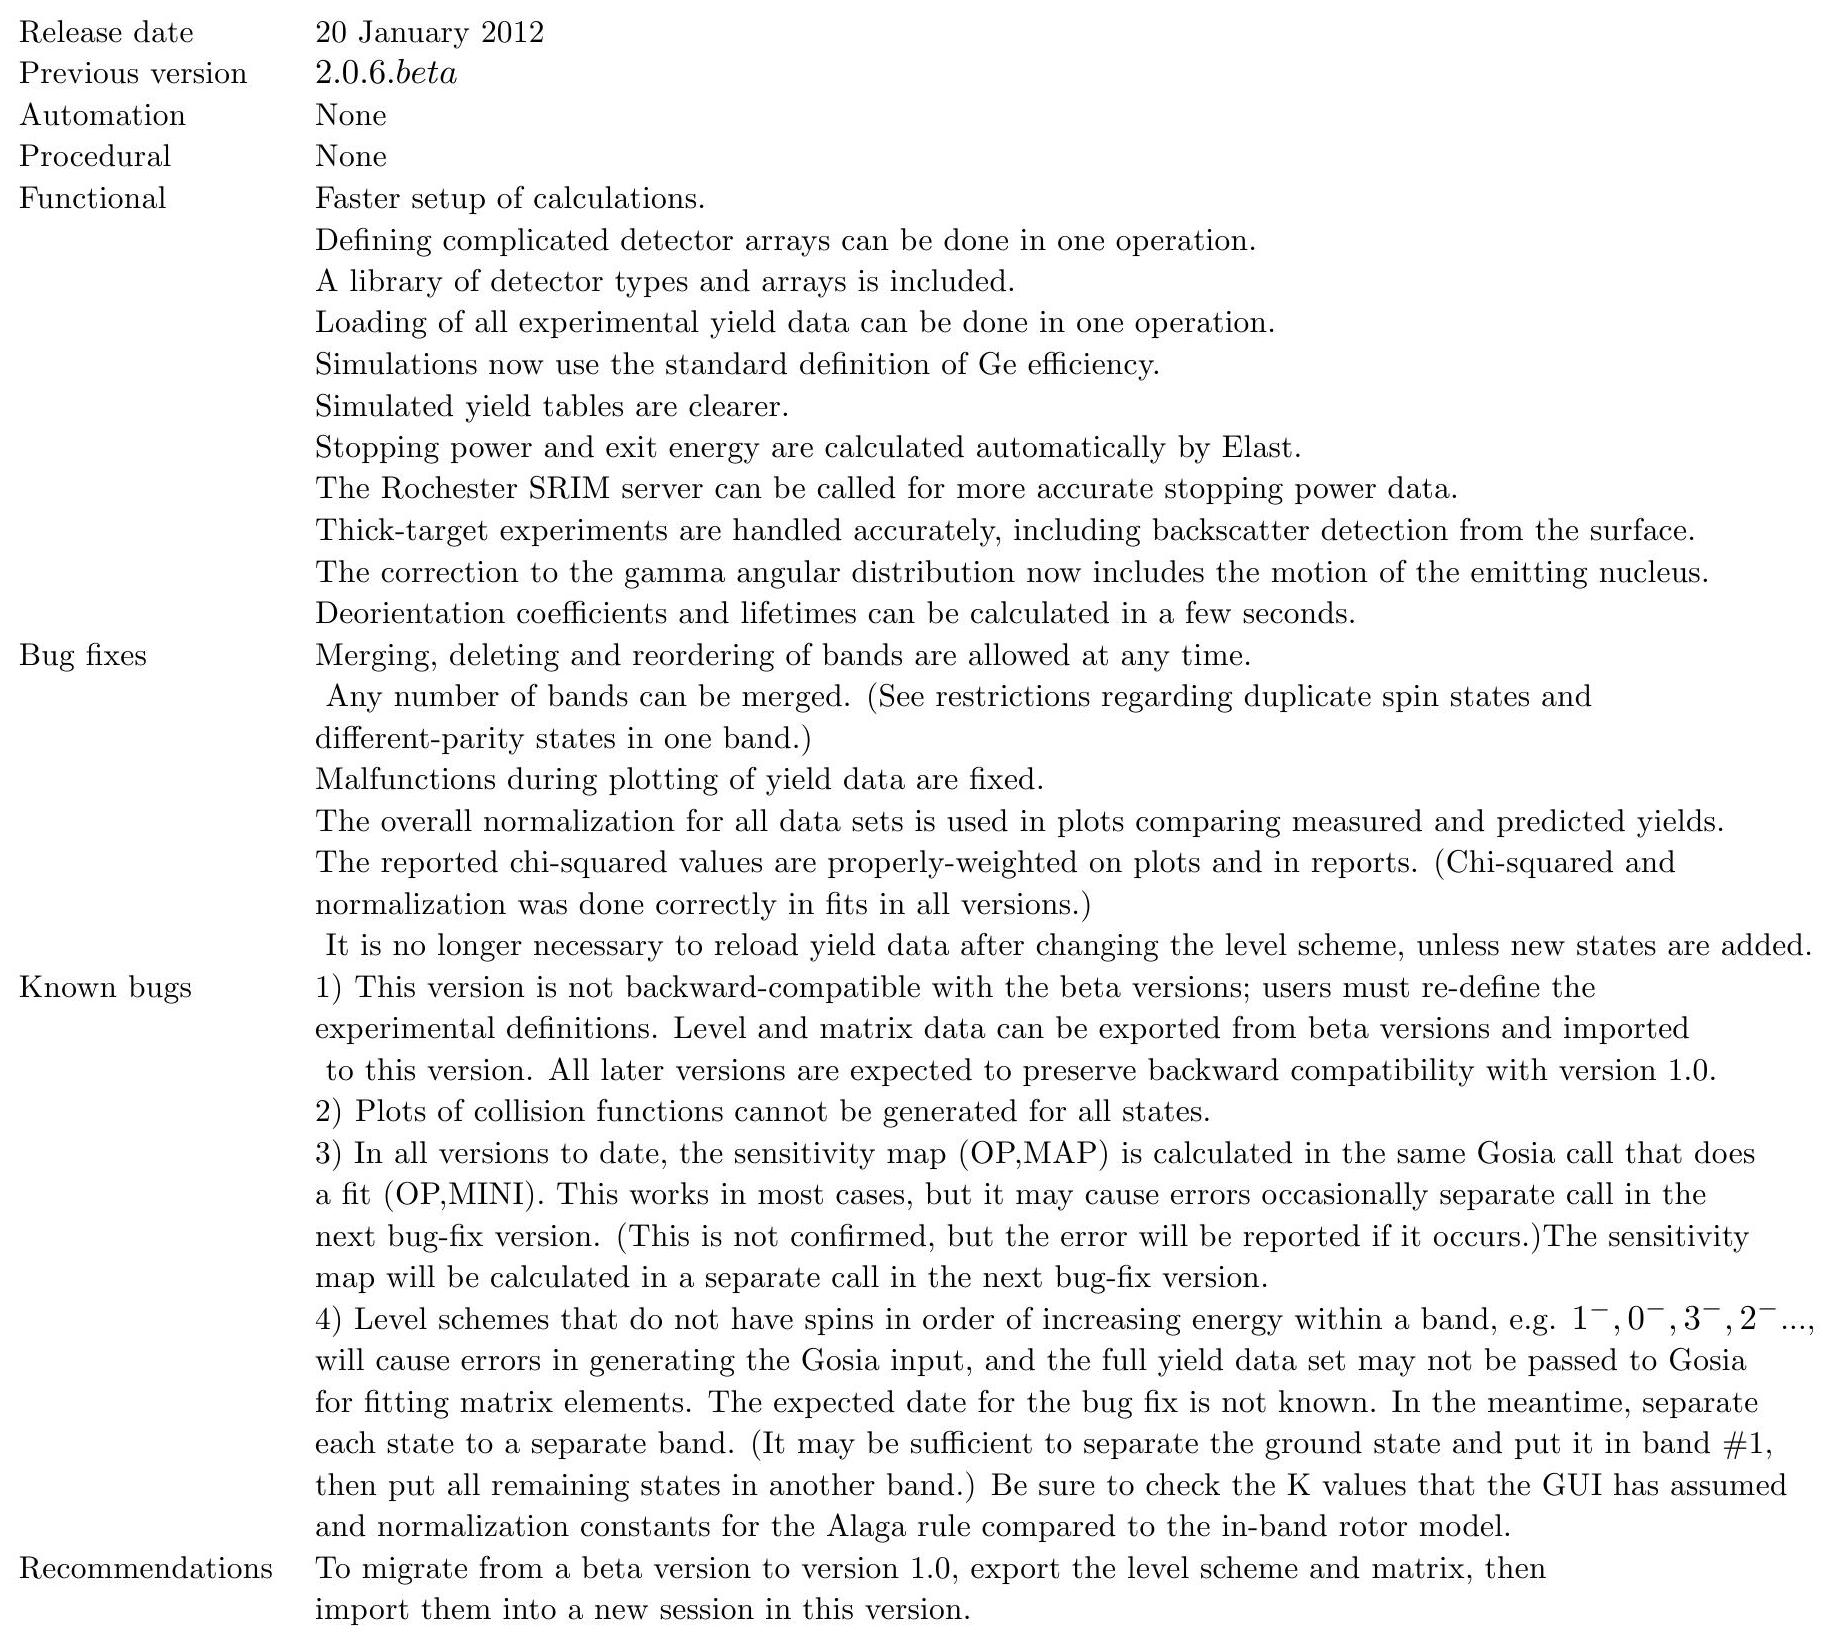
\includegraphics[max width=\textwidth]{2025_02_07_204a351db2d7f48b61ebg-294}
\end{center}

\subsection*{16.8.2 Version 2.0.6.beta}
\begin{center}
\begin{tabular}{ll}
Release date & 3 June 2011 \\
Previous version & 2.0 .5. beta \\
Automation & None \\
Procedural & None \\
Functional & None \\
Bug fixes & \begin{tabular}{l}
A bug that would overwrite \\
the calculated yields in memory with inaccurate point \\
calculations when using "View gosia input" or "Save gosia \\
input" is fixed. \\
\end{tabular} \\
 & \begin{tabular}{l}
Some collision functions cannot be plotted for all $\lambda, \mu$ values. \\
\end{tabular} \\
Known bugs &  \\
\end{tabular}
\end{center}

\subsection*{16.8.3 Version 2.0.5.beta}
\begin{center}
\begin{tabular}{ll}
Release date & 26 May 2011 \\
Previous version & 2.0.4.beta \\
Automation & None \\
Procedural & None \\
Functional & \begin{tabular}{l}
1. The user is now given the safe energy before \\
the prompt for the beam energy. \\
\end{tabular} \\
 & \begin{tabular}{l}
2. More information is provided when defining experiments to help the user avoid \\
scattering angles that will cause the integration to diverge. \\
\end{tabular} \\
 & \begin{tabular}{l}
3. The user is informed about which kinematic solutions will be included by Gosia \\
for inverse kinematics experiments. \\
\end{tabular} \\
Bug fixes & \begin{tabular}{l}
Attempted to fix a bug that would overwrite \\
the calculated yields in memory with inaccurate point \\
calculations when using "View gosia input" or "Save gosia \\
\end{tabular} \\
 & \begin{tabular}{l}
input". The bug remains in version 2.0.5.beta and is fixed in version 2.0.6.beta. \\
Known bugs \\
\end{tabular} \\
Some collision functions cannot be plotted for all $\lambda, \mu$ values. &  \\
\end{tabular}
\end{center}

\subsection*{16.8.4 Version 2.0.4.beta}
\begin{center}
\begin{tabular}{|c|c|}
\hline
Release date & 27 April 2011 \\
\hline
Previous version & 2.0.0.beta \\
\hline
Automation & Automated modification of session files from earlier beta-test version \\
\hline
Procedural & \begin{tabular}{l}
1. The sequence of prompts for experimental setup and data normalization have changed. \\
2. The user must select the forward or backward c.o.m. solution for inverse kinematics experiments with projectile detection, to match the calculations done by Gosia. \\
3. The user can now generate total counts in simulations, which requires several new prompts for experimental parameters. \\
4. The sequence of prompts in defining the laboratory experiments has changed to accommodate more detector shapes and data partitions over particle scattering angle. \\
\end{tabular} \\
\hline
Functional & \begin{tabular}{l}
1. The user is now informed on how to overcome a Gosia error, "...exceeds maximum scattering angle." \\
2. Accurate solid angles are calculated for Ge detectors. This is used primarily in simulating data, because relative yields are used in fits. \\
3. Diagonal errors may now be calculated separately and used to improve the chi-squared minimum. \\
4. Rectilinear detector shapes and azimuthally segmented detectors are now handled. \\
5. New warnings and guidance are now issued with the user prompts. \\
\end{tabular} \\
\hline
Bug fixes & \begin{tabular}{l}
1. A rounding error in the reduced chi-squared values on plots is fixed. \\
2. The calculation to determine which states are populated is robust for inverse kinematics cases. \\
3. A bug that prevented all nuclear data from being displayed and printed to the terminal is now fixed. \\
4. Several plotting bugs are fixed in the calls to gnuplot. \\
5. Fixed a bug in the error bars assigned to simulated data. \\
6. The sommerfeld parameters reported in "Examine setup" have been corrected. \\
\end{tabular} \\
\hline
Known bugs & Some collision functions cannot be plotted for all $\lambda, \mu$ values. \\
\hline
\end{tabular}
\end{center}

\subsection*{16.8.5 Version 2.0.0.beta}
\begin{center}
\begin{tabular}{ll}
Release date & 22 March 2011, Manual and videos created. \\
Previous version & $1 . * . *$.beta \\
Automation & Automated modification of session files from earlier beta-test versions. \\
Procedural & None \\
Functional & 1. Processes started with the "Go" button call Gosia to determine which states are \\
 & populated, which are isomers or have no decay path. Selection of data sent to Gosia \\
 & is automated correctly. \\
 & 2. A complete set of nuclear data is read from an external "human-readable" text \\
 & \begin{tabular}{l}
file and passed to Gosia as appropriate. \\
 \\
\end{tabular} A complete set of nuclear data is read and passed to Gosia as appropriate. \\
\end{tabular}
\end{center}

\subsection*{16.9 Chronology of Major Changes to the GOSIA Manual}
\section*{1 May 2012:}
\begin{enumerate}
  \item The RACHEL description is updated to match the newly released code RACHEL 1.0
  \item A $\gamma$-ray detection efficiency tensor approach has been developed to handle complicated $\gamma$-ray detector geometries that do not have cylindrical symmetry. Chapter 4.6 discusses the method, the usefulness of assuming axial symmetry, and of treating a complicated geometry as a cluster of axially-symmetric individual detectors. The OP.RAW, chapter 7.21, description has been changed to reflect using it to handle clusters of $\gamma$-ray detectors for which the experimental $\gamma$-ray yields have been corrected for the detection efficiency.
  \item Chapter 5.2 was expanded to emphasize the importance of including the $Q$-value dependence when making the transformation from the laboratory scattering angles to the corresponding centre-of-mass scattering angles for the states of interest. This is especially important when one of the interacting nuclei has a low mass.
  \item Chapter 5.3 reviews the $\approx 15 \%$ systematic errors and interpolation errors in available compilations and codes of stopping powers for heavy-ion energy loss in matter. It is recommended that SRIM be adopted for calculation of energy-loss stopping powers. Small changes have been made to chapter 7 and access to the SRIM code has been provided for RACHEL users.
  \item The magnitude of the systematic errors introduced by the $Q$-value dependence of the kinematics plus the systematic errors in energy loss compilations were included in the discussion of systematic errors in Chapter 6.81.
  \item Many typographic errors were corrected in the text. Typing errors in table 3.1 have been corrected.
\end{enumerate}

\section*{30 July 2011:}
\begin{enumerate}
  \item Major reorganization and inclusion of coauthor names
  \item Revised section on observables and absolute count rates in chapters 6 and 7 .
  \item Elucidated the Q-value dependence of the centre-of-mass angle, and Coulomb trajectory, at a given laboratory angle in chapters 5 and 6 .\\
8 June 2011:
  \item Typing errors in equations $4.5,5.12$, and 5.13 were corrected.
  \item RACHEL upgrade to 2.0.6.beta was included in Chapter 16.
\end{enumerate}

27 April 2011: New version of the Gosia Manual

\begin{enumerate}
  \item Major reorganization and revision of the Manual
  \item Included a description of the RACHEL GUI.
  \item Elucidated the adiabaticity limitations of the present version of Gosia.
  \item Included description of the OP,INTI solution to a inverse-kinematics problem.
  \item Added a section on planning Coulomb excitation experiments.
  \item Added an index to facilitate locating topics.
\end{enumerate}

\section*{14 April 2009:}
\begin{enumerate}
  \item Many editorial corrections to manual
  \item Expanded description of relativistic transformation of the angular distribution,
\end{enumerate}

30 June 2008:

\begin{enumerate}
  \item Includes increase in size of arrays.
  \item Restructure of EFFIX to allow more flexible selection of efficiency calibration type.
  \item Addition of Radware efficiency calibration
  \item Allow calling of LAGRAN or SPLNER to perform interpolation
\end{enumerate}

\section*{12 June 2008:}
\begin{enumerate}
  \item Added a section on kinematics,
  \item Several editorial corrections to improve presentation.
\end{enumerate}

\section*{20 May 2008:}
\begin{enumerate}
  \item Listed all members of the Gosia Users Steering Committee and their institutions.
  \item Added a dedication page to Tomasz Czosnyka,
\end{enumerate}

\section*{16 May 2008:}
\begin{enumerate}
  \item Added section 2.2 .4 on the calculation of internal conversion coefficients including addition of E0 conversion.
  \item Corrected a comment at end of OP,RE regarding requiring it to immediately preceed OP,ERRO or OP,MINI
\end{enumerate}

\section*{5 May 2008:}
\begin{enumerate}
  \item Updated the Introduction to separate the introduction from the history and manual description.
  \item Added section 2.2.4 "Sources of Systematic Error".
  \item Corrected input descriptions to correspond to the current version of Gosia.
  \item Added a description of the output from OP,GDET.\\
5)Chapter 11 "Learning Gosia", updated to include more sample inputs and corresponding outputs.
\end{enumerate}

2 April 2008:\\
Updated the Manual to correct an error in OP,INTG to reflect the fact that the maximum dimension of NI2 is 50 , not 100 . Also revised the Introduction and Release Notes chapters of the manual plus corrected typing errors in CONT and the Rotational Invariants chapter 6.

\section*{8 Oct 2007:}
Chapter 11 in the Gosia Manual changed to include a tutorial and instructions for compiling and using\\
GOSIA. Release Notes added to manual as chapter 13. Some minor editorial changes made to the GOSIA\\
Manual. Posted the latest 2007 version of GOSIA code plus the accuracy-speed-test.tar and g1demo.tar input/output files used by the GOSIA tutorial described in chapter 11.

\section*{30 Aug 2007:}
Updated the manual description of how to evaluate absolute counts using OP,POIN or OP,INTG

\section*{20 Aug 2007:}
Upgraded the GOSIA Manual to include the code GREMLIN

\section*{26 Feb 2007:}
Updated the manual regarding accuracy problems associated with large adiabaticity. Added a chapter\\
11 on accuracy, speed and compiling options.

\section*{25 Feb 2007:}
A new test input with associated output file and read me file were created that illustrate the accuracy, speed and compiling options for GOSIA.

\section*{20 Feb 2007:}
Corrected error in input instructions for ME in OP. YIEL.\\
6 Dec 2006:\\
Corrected typing errors in OP, MINI input\\
24 Aug 2006:\\
Added Drew Whitbeck comments to manual on input for GOSIA2.

\section*{13 June 2006:}
Corrected ICC description in OP,YIEL to include use of four point interpolation and increase in number of ICC energies to 50 .

\section*{9 June 2006:}
\begin{enumerate}
  \item ICC description in OP.YIEL revised with warning about how to handle ICC at energies near the K,L edges.
  \item Inserted the PIN diode option in CONT and OP.INTG.
  \item Added a very short comment about PAWEL.
\end{enumerate}

30 May 2006: Major update of the GOSIA Manual:

\begin{enumerate}
  \item Includes GOSIA2 for handling simultaneous Coulex of radioactive beams.
  \item All equations and chapter numbers in manual incremented by one
  \item Corrected figure 2.1 to coord B
  \item Added description of Ibbotson annealing code approach to minimization
  \item Added comments to aid in calculating total cross sections to OP.INTG
  \item Update OP.YIEL to include 1997 update allowing input of matrix elements for all multipolarities.
  \item Added description of OP,THEO to calculate rotational mode E2 matrix elements
\end{enumerate}

1990: Manual converted to Latex

\begin{enumerate}
  \item Previous MASS11 typeset version of Gosia Manual converted to Latex.
  \item The Gosia Manual was released to users as a pdf file.
\end{enumerate}

Oct 1985: First full typed version of the Gosia Manual

\begin{enumerate}
  \item The first full version of the Gosia Manual was written.
  \item The Manual was typeset using the VAX11 word-processing program MASS11.
\end{enumerate}

3 November 1980:\\
A brief handwritten set of input instructions for Gosia were written by Tomasz Czosnyka.

Please contact the members of the Gosia Steering Committee to report errors or suggestions regarding the Gosia User Manual. The Editor of the Gosia Manual can be reached at:

Douglas Cline,\\
Department of Physics and Astronomy,\\
University of Rochester,\\
Rochester, NY 14627, U.S.A.\\
Phone (585)275-4934.\\
\href{mailto:Email:Cline@pas.rochester.edu}{Email:Cline@pas.rochester.edu}.

\section*{Bibliography}
[ABR53] A. Abragam, R.V. Pound - Phys. Rev. 92:943 (1953)\\[0pt]
[ABR72] M. Abramowitz, I. Stegun (eds.) - Handbook of Mathematical Functions, National Bureau of Standards, Washington (1972)\\[0pt]
[ALD56] K. Alder, A. Bohr, T. Huus, B. Mottelson, A. Winther - Rev. Mod. Phys. 28:432 (1956)\\[0pt]
[ALD60] K. Alder, A. Winther, K. Dan. Vidensk, Selsk., Mat. Fys. Medd. 32, Number 8, (1960)\\[0pt]
[ALD66] K. Alder, A. Winther - Coulomb Excitation, Academic, New York, (1966)\\[0pt]
[ALD75] K. Alder, A. Winther - Electromagnetic Excitation, Theory of Coulomb Excitation with Heavy Ions, North Holland, Amsterdam, (1975)\\[0pt]
[BOE68] J. de Boer, J. Eichler; Advances in Nuclear Physics, Vol. 1, Plenum Press, p1\\[0pt]
[BOE84] J. de Boer, Treatise on Heavy-Ion Science, Vol. 1, Plenum Press, 1984, p293\\[0pt]
[BOH69] A. Bohr, B. Mottelson - Nuclear Structure, Benjamin, New York, (1969)\\[0pt]
[BOS77] F. Bosch, H. Spehl - Z. Phys. A280:329 (1977)\\[0pt]
[BRE77] R. Brenn, H. Spehl, A. Weckherlin, H. Doubt, G. Van Middelkoop - Z. Phys. A281:219 (1977)\\[0pt]
[BRI55] G. Breit, J.P. Lazarus, Phys. Rev. 100 (1955) 942\\[0pt]
[CHU56] E.L. Church and J. Weneser, Phys. Rev. 103 (1956) 1035\\[0pt]
[CLI69a] D. Cline, H.S. Gertzman, H.E. Gove, P.M.S. Lesser, J.J. Schwartz, Nucl. Phys. A133 (1969) 445\\[0pt]
[CLI69b] D. Cline - Bull. Am. Phys. Soc. 14:726 (1969)\\[0pt]
[CLI72] D. Cline, C. Flaum - Proc. Int. Conf. on Nucl. Struct. Studies using Electron Scatt. and Photoreaction, Sendai 1972, K. Shoda and H. Ui (eds.), Tohoku Univ. (1972)\\[0pt]
[CLI73] D. Cline, Journ. Phys. Soc. of Japan, 34 (1973) 377\\[0pt]
[CLI74] D. Cline, P.M.S. Lesser, C. Towsley; unpublished\\[0pt]
[CLI86] D. Cline - Ann. Rev. Nucl. Part. Sci. 36:683 (1986)\\[0pt]
[CLI08] D. Cline, A.B. Hayes, Internal GOSIA Memorandum, December 2008\\[0pt]
[CLIN12] D. Cline, "Classical Mechanics" Draft of a textbook 2012\\[0pt]
[CO06] J.M. Cook, T. Glasmacher, A. Gade, Phys. Rev. C73 (2006) 024315\\[0pt]
[CZO83] T. Czosnyka, D. Cline, C.Y. Wu - Am. Phys. Soc. 28:745 (1983)\\[0pt]
[CZO83b] T. Czosnyka, D. Cline, C.Y. Wu, GOSIA Manual, NSRL Report, University of Rochester, 1983\\[0pt]
[Du90] G. Dueck, T. Scheuer, J. Comp. Phys. 90 (1990) 161.\\[0pt]
[FER65] A.J. Ferguson, "Angular Correlation Methods in Gamma-Ray Spectroscopy", (North Holland Publishing Company,1965)\\[0pt]
[FRA65] H. Frauenfelder, R. Steffen - in Alpha-, Beta and Gamma Spectroscopy, K. Siegbahn (ed), North Holland, Amsterdam, (1965)\\[0pt]
[Ge84] S. Geman and D. Geman, IEEE Trans. Patt. Anan. Mach. Int. PAM1-6 (1984) 721.\\[0pt]
[GER70a] H.S. Gertzman, D. Cline, H.E. Gove, P.M.S. Lesser, J.J. Schwartz, Nucl. Phys. A151 (1970) 273\\[0pt]
[GER70b] H.S. Gertzman, D. Cline, H.E. Gove, P.M.S. Lesser, Nucl. Phys. A151 (1970) 282\\[0pt]
[GL98] T. Glasmacher, Ann. Rev. Nucl. Part. Sci. 48 (1998) 1\\[0pt]
[GL01] T. Galsmacher, Nucl. Phy. A693 (2001) 90\\[0pt]
[GOL77] G. Goldring, private communication\\[0pt]
[GOL78] G. Goldring, K.Hagermeyer, N. Benczer-Koller, R. Levy, Y. Lipshitz, B. Richter, Z. Shkedi, Y. Wolfson, K.H. Speidel, Hyperfine Interactions, 5 (1978) 283\\[0pt]
[GOLD02] H. Goldstein, C. Poole, J. Safko, "Classical Mechanics", (Addison Wesley, 2002)\\[0pt]
[GOS08] GOSIA website (2008), \href{http://www.pas.rochester.edu/~cline/Research/GOSIA.htm}{http://www.pas.rochester.edu/\~{}cline/Research/GOSIA.htm}.\\[0pt]
[GRE72] S. Green, Phys. Rev. A4 (1972) 251\\[0pt]
[GRE84] H. Grein, H. Emling, J. Stachel - GSI Rep. GSI-84-1 (1984)\\[0pt]
[GS98] Gammasphere online documentation (1998), \href{http://www.phy.anl.gov/gammasphere/doc/efficiency}{http://www.phy.anl.gov/gammasphere/doc/efficiency}.\\[0pt]
[GUI76] M.W. Guidry, P.A. Butler, P. Columbani, I-Y. Lee, D. Ward, et al, Nuclear Physics, A266 (19760228\\[0pt]
[HAG63] R. Hagedorn, "Relativistic Kinematics" (Benjamin, Inc NY 1963)\\[0pt]
[HAS80] L. Hasselgren and D. Cline; Proceeding of the International Conference on Interacting Bose-Fermi Systems in Nuclei, Ed. F. Iachello, Plenum Press (1981) p. 59\\[0pt]
[HAY07] A.B. Hayes, D. Cline, K.J. Moody, C.Y. Wu, et al, Laser Physics 17 (2007) 745\\[0pt]
[HAY10] A.B. Hayes, D. Cline, K.J. Moody, I. Ragnarsson, et al, Phys. Rev. C82 (2010) 044319\\[0pt]
[HAY10b] A.B. Hayes, D. Cline, C.Y. Wu, A.M. Hurst, M.P. Carpenter,J.P. Greene, R.V.F. Janssens, T. Lauritsen, D. Seweryniak, S. Zhu, S.A. Karamanian, P.M. Walker, T.P.D. Swan, S.V. Rigby, D.M. Cullen, N.M. Lumley, P. Mason, J.J. Carroll, B. Detwiler, T. Harle, I. Mills, G. Trees; International Journal of Modern Physics, E, In press (2010)\\[0pt]
[IBB95] R.W. Ibbotson, Ph.D. Thesis, University of Rochester, 1995.\\[0pt]
[In89] L. Ingber, Math.. Comput. Modelling 12 (1989) 967.\\[0pt]
[KAV90] A. E. Kavka, Ph.D. Thesis, University of Uppsala, 1990\\[0pt]
[KIB08] T. Kibédi, T.W. Burrows, M.B. Trzhaskovskaya, P.M. Davidson, C.W. Nestor, Nucl. Instr. Meth. A589 (2008) 202\\[0pt]
[Ki83] S. Kirkpatrick, C. D. Gelatt Jr. and M. P. Vecchi, Science 220 p 671 (1983).\\[0pt]
[KOT84] B. Kotlinski, Ph.D. Thesis, University of Rochester, 1984\\[0pt]
[KOT89] B. Kotlinski, A. Backlin, D. Clark, D. Cline, Nuclear Physics, A503 (19890 575\\[0pt]
[KRA70] K. Krane, R. Steffen - Phys. Rev. C2:724 (1970)\\[0pt]
[KRA72] K. Krane - Nucl. Instr. Meth. 98:205 (1972)\\[0pt]
[KUM71] K. Kumar, Private communication, (1971)\\[0pt]
[KUM72] K. Kumar, Phys. Rev. Letts. 28 (1972) 249\\[0pt]
[LEE77] I.Y. Lee, D. Cline, P.A. Butler, R.M. Diamond, J.O. Newton, R.S. Simon and F.S. Stephens; Phys. Rev. Lett. 39 (1977) 684.\\[0pt]
[LEE81] P.A.Lee, P.H. Citrin, P. Eisenberger, B.M. Kinkaid, Rev. Mod. Phys. 53 (1981) 769\\[0pt]
[LEL78] A. Lell, Diplomarbeit, Sektion Physik, Universität München (1978)\\[0pt]
[LES70] P.M.S. Lesser, D. Cline, J.D. Purvis, Nucl. Phys. A151 (1970) 257\\[0pt]
[LES72] P.M.S. Lesser, D. Cline, P. Goode, R. Horoshko, Nucl. Phys. 28 (1972) 368\\[0pt]
[LES71] P.M.S. Lesser - PhD Thesis, Univ. of Rochester (1971)\\[0pt]
[LES74] P.M.S. Lesser, D. Cline, C.K. Cline, A. Bahnsen, Nucl. Phys. A223 (1974) 563\\[0pt]
[LES10] P.M.S. Lesser, D. Cline, Nuclear Instruments and Methods, A614 (2010) 41\\[0pt]
[MA78] M.H. Macfarlane, S.C. Pieper, Argonne Nat. Lab. Report, ANL-76-11 Rev. 1 (1978)\\[0pt]
[MCG69] F.K. McGowan, Proc. of the heavy-ion Summer Study Group, Ed; S.T. Thornton, Oak Ridge National Laboratory (1969) p38\\[0pt]
[Me53] N. Metropolis, A.W. Rosenbluth, M.N. Rosenbluth, A.H. Teller, E. Teller, J. Chem. Phys. 21 (1953) 1087.\\[0pt]
[ME61] E. Merzbacher, "Quantum Mechanics" (John Wiley, N.Y., 1961)\\[0pt]
[MET70] F.R. Metzger, Nucl. Phys. A148 (1970) 362\\[0pt]
[Mo90] P. Moscato and J.F. Fontanari, Phys. Lett. A146 (1990) 204.\\[0pt]
[NED03] A. Quirantes, ned code, version 20 May 2003, \href{http://www.ugr.es/~aquiran/codigos.htm}{http://www.ugr.es/\~{}aquiran/codigos.htm}.\\[0pt]
[NIK68] V.S. Nikolayev, I.S. Dmitriev - Phys. Lett. 28A:277 (1968)\\[0pt]
[NNDC] National Nuclear Data Center online databases (Accessed March 9, 2011), \href{http://www.nndc.bnl.gov}{http://www.nndc.bnl.gov}.\\[0pt]
[NOR70] L.C. Northcliffe, R.F. Schilling; Nuclear Data Tables A7 (1970) 233\\[0pt]
[PAU03] H. Paul, A. Schinner, Nucl. Inst. and Meth. in Phys. Res. B209 (2003) 252\\[0pt]
[PRE92] W.R. Press, S.A. Teukolsky, W.T. Vetterling, B.P. Flannery, "Numerical Recipes in Fortran", Cambridge University Press, 1992\\[0pt]
[RH80] M. Rhodes-Brown, M.H, Macfarlane, S.C. Pieper, Phys. Rev C21 (1980) 2417\\[0pt]
[ROS53] M.E. Rose, Phys. Rev. 91 (1953) 610\\[0pt]
[ROT59] M. Rotenberg, R. Bivins, N. Metropolis, J. Wooten - The 3j and 6j Symbols, The Technology Press, Cambridge, Mass. (1959)\\[0pt]
[Sa91] Algorithmica 6 (1991) 295. (Special Edition on Simulated Annealing edited by A. SangiovanniVincentelli)\\[0pt]
[SIM97] M.W. Simon, D. Cline, C.Y. Wu, R. Gray, R. Teng, C. Long; Nuclear Instruments and Methods, A452 (2000) 205\\[0pt]
[STA82] J. Stachel, N. Kaffrell, E. Grosse, H. Emling, H. Folger, R. Kulessa, D. Schwalm, Nucl. Phys. A383 (1982) 429\\[0pt]
[Sz87] H. Szu and R. Hartley, Phys. Lett. A122 (1987) 157.\\[0pt]
[STO05] N.J. Stone, A.E. Stuchberry, M. Danchev, J. Pavan, et al; Eur. Phys. J. A25 (2005) 205\\[0pt]
[TOL79] L.D. Tolsma, Phys. Rev. C20 (1979) 592\\[0pt]
[TOL87] L.D. Tolsma, Phys. Rev. C35 (1987) 177\\[0pt]
[TOW72] C. Towsley, D. Cline, R. Horoshko, Phys. Rev. Letts. 28 (1972) 368\\[0pt]
[TOW73] C. Towsley, D. Cline, R. Horoshko, Nucl. Phys. A204 (1973) 574\\[0pt]
[TOW75] C. Towsley, D. Cline, R. Horoshko, Nucl. Phys. A250 (1975) 381\\[0pt]
[VAR86] B. Varnestig, A. Backlin, C. Fahlander, A. Kavka, T. Lenke, L.E. Svensson - Nucl. Instr. Meth. A248:419 (1986)\\[0pt]
[VER74] W.J. Vermeer, M.T. Esat, M. Fewell, R.H. Speer, A.M. Baxter, S.M. Burnett, Phys. Letts. 138 (1984) 365\\[0pt]
[1] \href{http://en.wikipedia.org/wiki/Table_of_spherical_harmonics}{http://en.wikipedia.org/wiki/Table\_of\_spherical\_harmonics}\\[0pt]
[WAR76] D. Ward, P. Columbani, I-Y. Lee, P.A. Butler, R.S. Simon, et al, Nuclear Physics, A266 (1976) 194\\[0pt]
[WAR05] D. Ward, R.M. Clark, M. Cromaz, M.A. Delaplanque, R.M. Diamond, P. Fallon, G.J. Lane, I.Y. Lee, A. Georgen, A.O. Macchiavelli, F.S. Stephens, C.E. Svensson, K. Vetter, D. Cline, A.B. Hayes, R. Teng, C.Y. Wu, T. Nakatsukasa; "Nuclei at the Limits" AIP Conf. Proc. 764 (2005) 263\\[0pt]
[WAR12] D. Ward, A.O. Macchiavelli, R.M. Clark, D. Cline, M. Cromaz, M.A. Delaplanque, R.M. Diamond, P. Fallon, G.J. Lane, I.Y. Lee, A. Georgen, A.B. Hayes, T. Nakatsukasa, R. Teng, G. Schmidt, F.S. Stephens, C.E. Svensson, K. Vetter, C.Y. Wu; Phys. Rev, C, To be submitted 2012.\\[0pt]
[WAR08] N. Warr, Internal GOSIA Memorandum, December 2008\\[0pt]
[WIN65] A. Winther and J. de Boer, 1965, A Computer Program for Multiple Coulomb Excitation, California Institute of Technology, Technical Report, reprinted in [ALD66]\\[0pt]
[WU83] C-Y Wu, Ph.D. Thesis, University of Rochester, 1983\\[0pt]
[WU89] C-Y. Wu, D. Cline, E.G. Vogt, W.J. Kernan, T. Czosnyka, A.E. Kavka, R.M. Diamond, Phys. Rev. C40 (1989) R3\\[0pt]
[WU91] C-Y. Wu, D. Cline, E.G. Vogt, W.J. Kernan, T. Czosnyka, A.E. Kavka, B. Kotlinski, R.M. Diamond, Nucl. Phys. A533 (1991) 369\\[0pt]
[WU96] C-Y. Wu, D. Cline T. Czosnyka, A. Backlin, C. Baktash, R.M. Diamond, G.D. Dracoulis, L. Hasselgren, H. Kluge, B. Kotlinski, J.R. Leigh, J.O. Newton, W.R. Phillips, S.H. Sie, J. Srebrny, FG.S. Stephens; Nucl. Phys. A607 (1996) 178\\[0pt]
[WU00] C.Y. Wu, D. Cline, M.W. Simon, R. Teng, K. Vetter, M.P. Carpenter, R.V.F. Janssens, I. Wiedenhover; Physical Review C61 (2000) 021305 (R)\\[0pt]
[WUE03] M. Wuerkner, J. de Boer, A.I. Levon, M. Loewe, J. Kvasil, J. Srebrny, P.J. Napiorkowski, J. Iwanicki, T. Czosnyka; Nucl. Phys. A725 (2003) 3\\[0pt]
[ZIE08] J.F. Ziegler, J.P. Biersack, M.D. Ziegler; "SRIM; Stopping and Range of Ions in Matter" SRIM Co, 2008\\[0pt]
[ZIE12] J.F. Ziegler, Private communication, 2012.

\section*{Index}
$A C C, X . \quad$ accuracy parameter, 121\\
$A C P, X$. convergence test parameter, 121\\
$B\left(\lambda ; I_{k} \rightarrow I_{f}\right) \quad$ transition strength, 24,39\\
$C C F, \quad$ correction factor switch, 121\\
$C R D, X$. circular particle detector switch, 121\\
$C R F \quad$ read correction factors, 121\\
$D I P, X . \quad E 1$ polarization parameter, 122\\
$D_{\chi \chi^{\prime}}^{k}(\alpha, \beta, \gamma) \quad$ rotation matrix, 43\\
E0 decay width, 53\\
$E N D \quad$ mandatory CONT flag, 122\\
$E_{\max } \quad$ safe bombarding , 15\\
$E_{j}$ excitation energy (MeV) of index level, 152\\
$F I X, \quad$ fix matrix elements, 122\\
$F M I, \quad$ fast minimization switch, 122\\
$F_{k}\left(\lambda \lambda^{\prime}, I_{2} I_{1}\right) \quad$ correlation coefficient, 84\\
$G^{\text {fluct }}(t) \quad$ fluctuation attenuation coefficient, 46\\
$G_{k}(t) \quad$ deorientation coefficient, 45\\
$G_{k} \quad$ attenuation coefficient, 19\\
$G_{k}^{(s t a t)}(t) \quad$ static attenuation coefficient, 45\\
$I A X \quad$ axial symmetry flag, 133\\
$I C C(E \lambda) \quad$ internal conversion coefficient OP,BRIC, 120\\
ID1 number of $\gamma$ detectors in cluster 1, 165\\
IEXP Experiment number, 184\\
$I E X P \quad$ index number of raw experiment, 165\\
IFLAG Flag for recoil displacement correction, 177\\
IFL normal/simulation flag, 163\\
IKIN kinematics flag, 133\\
INDEX\# level index numbers, 154, 157\\
$I N R, \quad$ independent normalization switch, 122\\
$I N T, X$. integration step-size parameter, 122\\
$I P(J) \quad$ Identify physical Ge detectors in logical detectors, 178\\
$I P_{j} \quad$ index level parity, 152\\
$I_{j} \quad$ user given level index, 152\\
$K \quad$ Band $K$ value, 172\\
$L C K$, lock matrix element switch, 122\\
$L N$ normalization control flag, 133\\
$M E \quad$ reduxed matrix element, 154,157\\
$M_{0} \quad$ ground-state polarization, 72\\
$M_{A} \quad$ \# substates in approximate calculation, 133\\
$M_{C} \quad \#$ of substates in full calculation, 132\\
$N \quad$ number of experimental observables, 97,109\\
$N A N G(I) \quad \#$ of $\gamma$ detectors for each of $N E X P$ experiments, 178\\
$N B R A \quad$ number of branching ratios input, 178\\
$N C M, X$. kinematics state selection, 123\\
$N C \quad$ number of Ge clusters, 165\\
$N D L \quad$ Number of mixing ratios, 178\\
NDST 3 of data sets in given experiment, 178\\
$N D \quad$ Number of expt $\gamma$ yields for IEXP, 184\\
$N E \quad$ number of energy meshpoints, 137, 145\\
NFI number of $\phi$ ranges for each $\theta, 138,146$\\
$N G \quad$ Number of data sets for IEXP, 184\\
NLEV Number of levels in $K$ band., 172\\
$N L \quad$ Number of lifetimes input, 178\\
$N P \quad$ number of stopping powers, 138,146\\
NTAP Specify file containing expt data, 178\\
$N T A P \quad$ experimental yields file $\#, 127$\\
$N T \quad$ number of $\theta$ meshpoints, 137, 146\\
PIN, X. pin-diode detector option, 123\\
PRT, print options, 123\\
$P_{k \chi} \quad$ Legendre spherical function, 84\\
$P_{k} \quad$ excitation probability, 34\\
$Q(\epsilon, \omega) \quad$ collision function, 35,71\\
$Q^{2} \quad E 2$ rotational invariant, 220\\
$Q_{k} \quad$ attenuation coefficient, 84\\
$R_{1} R_{2} \quad$ m.e. lower and upper limits, 157\\
$R_{\lambda \mu}(\epsilon, \xi) \quad$ orbital integral, 38,80\\
$R_{k \chi}\left(I, I_{f}\right) \quad$ angular distribution tensor, 43, 84\\
$S(\bar{M}) \quad$ normalized least-squares statistic, 110\\
$S E E D$ random number seed, 164\\
$S E L, \quad$ create OP,SELE file, 125\\
$S K P, X$. skip X experiments, 125\\
$S M R, \quad$ SIGMA code control switch, 126\\
$S P L, X$. spline control switch, 126\\
$S_{j} \quad$ spin of the index level, 152\\
TEN, output statistical tensors, 126\\
$U P L_{j} \quad$ Upper detection limit of detector $j, 178$\\
$V(t) \quad$ interaction potential, 34\\
$V A C, \quad$ vacuum deorientation parameters, 126\\
$W B R A \quad$ weights for branching ratio, 178\\
$W D L \quad$ Weights for branching ratios, 178\\
$W L \quad$ Weights for lifetimes, 178\\
$W R N, X$. fit error warning, 126\\
$W T \quad$ Weighting factor for experiment, 184\\
$Y\left(\left(I \rightarrow I_{f}\right), \theta_{p}, E\right) \quad \gamma$-ray point yields, 85

YLIM simulation sensitivity level, 163\\
$Y N R M_{j} \quad$ Relative normalization factors, 178\\
$Y_{\lambda \mu}(\theta(t), \phi(t)) \quad$ spherical harmonic, 34\\
$Y_{i}\left(I \rightarrow I_{f}\right) \quad$ integrated yields, 86\\
$\Gamma(E 0) \quad$ E0 decay width, 53\\
$\Gamma\left(I, I_{f}\right)_{\text {total }} \quad$ total decay width, 52\\
$\Gamma \quad$ Lamor frequency distribution width, 46\\
$\alpha \quad$ half distance of closest approach, 17\\
$\alpha_{k i}^{P} \quad$ sensitivity parameter, 25\\
$\alpha_{k i}^{p} \quad$ probability sensitivity parameter, 106\\
$\alpha_{k i}^{y} \quad$ yield sensitivity parameter, 105\\
$\alpha_{k} \quad$ excitation amplitude, 34\\
$\bar{j}(\bar{r}) \quad$ current distribution, 34\\
$\bar{r} \quad$ radius vector, 35\\
$\chi^{2} \quad$ penalty function, 69\\
$\chi^{2} \quad$ unnormalized least-squares statistic, 110\\
$\delta \quad E 2$ triaxiality invariant, 220\\
$\delta_{0} \quad E 0$ transition amplitude, 42\\
$\delta_{\chi_{0}} \quad$ Kronecker symbol, 84\\
$\delta_{\lambda} \quad$ transition amplitude, 42,84\\
$\epsilon \quad$ eccentricity, 79\\
$\epsilon \quad$ orbit eccentricity, 34\\
$\epsilon_{k \chi}$ detection efficiency tensor, 49\\
$\epsilon_{k \chi}^{F D}\left(E_{\gamma}\right) \quad$ finite-size detector efficiency tensor, 50\\
$\eta \quad$ Sommerfeld parameter, 17\\
$\gamma\left(I_{1}\right) \quad$ emission probability, 42\\
$\lambda \quad$ multipolarity, 154,157\\
$\omega \quad$ orbit parameter, 35\\
$\rho(\bar{r}) \quad$ charge distribution, 34\\
$\rho_{k \chi}(I) \quad$ statistical tensor, 41\\
$\xi_{k n} \epsilon \quad$ adiabaticity product, 79\\
$\xi_{k n} \quad$ adiabaticity parameter, 36, 79\\
$\zeta_{k n}^{(\lambda \mu)} \quad$ coupling parameter, 37\\
$c(\lambda) \quad$ internal conversion coefficient, 52\\
$d_{\chi \chi^{\prime}}^{k}(\beta) \quad$ rotation matrix for $\alpha=\gamma=0,43$\\
$F_{k}\left(\lambda \lambda^{\prime}, I_{2} I_{1}\right) \quad$ correlation coefficient, 42\\
$G_{k} \quad$ attenuation coefficient, 43\\
NI1 number of energy subdivisions, 139\\
NI1 number of equal energy subdivisions, 147\\
NI2 number of equal angle subdivisions, 139, 147\\
$Q_{k \chi}\left(E_{\gamma}\right) \quad$ solid-angle attenuation tensor, 50\\
$Q_{k}\left(E_{\gamma}\right) \quad$ solid-angle attenuation coefficient, 51\\
$S(\bar{M}) \quad$ normalized least-squares statistic, 97\\
$c(\lambda) \quad$ internal conversion coefficient, 44\\
$p\left(J_{i}\right) \quad$ atomic charge state distribution, 46\\
Absolute $p-\gamma$ yields, 93, 142, 150\\
Eccentricity $\quad \epsilon, 79$\\
$\gamma$-ray yields, 83\\
64-bit accuracy, 70\\
Absorption coefficients, 84\\
Accuracy test, 80, 83\\
Adams-Moulton predictor-corrector method, 71\\
Adiabaticity limitations, 79\\
Adiabaticity parameter, 36, 79\\
constraints, 19\\
Adiabaticity product, 79\\
Angular correlation, 42\\
Angular distribution\\
attenuation coefficients, 19\\
symmetry properties, 53\\
Angular distribution tensor, 43, 69\\
Atomic charge state, 46\\
Attenuation coefficient, 43, 84\\
angular distribution, 19\\
Branching ratio, 69\\
BrIcc\\
internal conversion coefficients, 53\\
Buffer states, 107, 194

\section*{CHICO}
heavy-ion detector, 21\\
CHILIM S criterion to stop minimization, 162\\
Chronology for GOSIA code, 291\\
Chronology for RACHEL code, 297\\
Chronology of GOSIA Manual, 297\\
Circular particle detector option, 140, 148\\
Collective model matrix elements, 188\\
Collision function, 35, 80\\
accuracy, 71\\
CONT\\
control suboption, 116, 257\\
CONT (CONTROL suboption), 121, 128, 136\\
CONV convergence criterion, 162\\
Coordinate frame\\
B, 34\\
C, 42\\
Corrected yields, 70\\
Correction factors, 69, 270\\
Coulomb excitation accuracy tests, 31\\
Coulomb-nuclear interference, 106 reorientation effect, 15\\
Coupled-channel equations, 70\\
Coupling parameter, 37\\
Cross section\\
absolute p-gamma yields, 142, 150\\
Current distribution, 34\\
Degrees of freedom, 108\\
Deorientation effect, 44 attentuation coefficient, 45\\
hyperfine interaction, 19 two-state model, 19\\
Diagonal errors error estimation, 111\\
Differential cross section, 84\\
Distance of closest approach, 17\\
DLOCKS Derivative limit to lock matrix elements, 162

Doppler effect\\
Doppler broadening , 21\\
Doppler correction, 22

\section*{ELAST}
stopping powers, 66, 191\\
Electric dipole polarization, 37\\
Electric monopole transition, 42\\
END\\
mandatory CONT suboption, 257\\
Erroneous data\\
OP,TROU, 113\\
Error estimation, 70, 106\\
correlated errors, 273\\
correlation axis, 112\\
diagonal errors, 112, 272\\
see systematic errors, 106\\
statistical error, 108\\
Error message\\
unrecognized option, 116\\
Excitation amplitude, 72\\
symmetry, 72\\
Excitation amplitudes, 34\\
Excitation probability, 34\\
Expansion failure, 79\\
Experimental gamma-ray yields input, 119\\
Experimental yield data\\
input ordering, 180\\
EXPT\\
experimental input suboption, 116, 117, 257\\
EXPT experimental parameters input, 128, 132, 136\\
Fast approximation, 74, 78\\
File assignments\\
GOSIA, 229\\
SELECT, 231\\
SIGMA, 231\\
Gamma-ray detectors order, 106\\
Gamma-ray yields, 85\\
Gammasphere, 21\\
, 188\\
Ge detectors\\
define geometry, 270\\
GOSIA\\
64-bit accuracy, 70\\
compile, 255\\
examples, 255\\
fitting matrix elements, 267\\
flow sequence, 258\\
input format, 115\\
learning, 255\\
new starting point, 272\\
simulation, 187\\
troubleshooting, 275

GOSIA2\\
input, 255\\
simultaneous excitation, 239\\
GREMLIN, 165\\
$\gamma$-ray detection efficiency, 279\\
detection-efficiency parameters for OP,RAW, 279\\
efficiency-corrected gamma yields, 279\\
two modes, 279\\
GRETINA\\
gamma-ray energy tracking array, 21\\
Ground-state polarization, 73\\
Hyperfine fields\\
static magnetic moments, 27\\
Hyperfine interaction, 43\\
deoriantation effect, 19\\
IDF error mode flag, 129\\
IFBL forward-backward difference flag, 162\\
IFC use correlation matrix flag, 130\\
IMODE minimization mode flags, 161\\
In-flight decay, 108\\
Input of experimental yields, 184\\
Integrated yields, 86\\
normalization, 87\\
units, 86\\
Integration\\
$\left(\theta_{p}, E\right)$ meshpoints, 86\\
Interaction potential, 34\\
Internal conversion coefficient, 44, 52\\
BrIcc tabulation, 53\\
Internal correction factors, 100\\
Inverse kinematics, 87, 137\\
IREP error repetition flag, 129\\
Isomer Coulomb excitation, 247\\
Kinematic coincidence, 62\\
Kinematics, 57\\
angle transformation, 58\\
recoil energies, 60\\
velocity transformation, 57\\
Least-squares minimization, 97\\
probability distribution, 110\\
Least-squares search\\
minimization, 97\\
Least-squares statistic, 69, 97\\
Legendre spherical function, 84\\
LEVE, 257\\
energy levels suboption, 116, 118\\
LEVE Levels suboption, 128, 136, 152\\
Lifetime, 69\\
LOCKF Automatically lock matrix elements, 162\\
LOCKS flag to lock matrix elements, 162\\
Logical experiments, 69

Magnetic substates, 69\\
Matrix approximation, 69\\
Matrix element\\
coupling, 157\\
fit parameters, 157\\
Matrix elements, 69\\
ME\\
matrix element input suboption, 116, 118, 257\\
ME (OP,COUL) matrix elements suboption, 128, 154\\
ME (OP,GOSI) matrix elements suboption, 136, 157\\
MiniBall, 21, 188\\
Minimization\\
convergence limit, 105\\
coupled matrix elements, 105\\
cpu time, 162\\
data inconsistencies, 113\\
diagonal errors, 111\\
erroneous data, 113, 114\\
erroneous local minima, 113\\
fast approximation, 113\\
forward-backward approximation, 102\\
global minimum, 113\\
gradient plus derivative, 102\\
identify erroneous data, 113\\
incorrectly assigned transitions, 113\\
least-squares, 70\\
least-squares search, 97\\
maximum correlation curve, 111\\
normalization constants, 113\\
numerical estimation of errors, 111\\
saddle points, 114\\
sensitivity maps, 105\\
steepest descent, 100\\
weighting factor, 182\\
yield sensitivity map, 112\\
Mixing ratio, 69\\
Multipole expansion, 34\\
Mutual excitation, 108\\
NBANDS (Number of user-defined bands), 172\\
NEXP Number of defined experiments, 132\\
NLOCK number of matrix elements locked by LOCKF, 162\\
Normalization\\
constants, 98,181\\
coupled experiments, 99\\
cross sections, 108\\
relative constants, 181\\
NPD (Number of types of Ge detectors), 135\\
NPTL Maximum number of minimiozation steps, 162\\
Nuisance parameters, 109\\
Numerical integration, 86\\
Observation limit, 98\\
OP,ANNL, 249\\
OP,BRIC\\
internal conversion coefficient module, 116\\
OP,BRIC (BRICC), 120\\
OP,CORR, 86\\
correct yields module, 116\\
OP,CORR (CORRECT), 100, 127\\
OP,COUL, 115\\
Coulex calculation option, 116\\
OP,COUL (COULEX option), 128\\
OP,ERRO\\
error estimation module, 116\\
OP,ERRO (ERROR estimation), 129\\
OP,EXIT\\
job termination option, 116\\
OP,EXIT (Terminate code execution), 131\\
OP,FILE, 257\\
declare file numbers, 117\\
OP,FILE (define permanent files), 134\\
OP,GDET\\
create Ge detector files, 117\\
OP,GDET (Define Ge detector properties), 135\\
OP,GOSI, 115, 257\\
Gosia matrix element fit code, 117\\
OP,GOSI (GOSIA fit option), 136\\
OP,INTG, 87\\
original yield integration routine, 117\\
OP,INTG (1980 integration suboption), 137\\
OP,INTI, 87\\
learning, 257, 273\\
new yield integration routine, 117\\
OP,INTI (2008 integration suboption), 145\\
OP,MAP\\
calculate q-parameter map, 118\\
OP,MAP (generate q map), 153\\
OP,MINI\\
minimization routine, 118\\
OP,MINI (Minimize), 161\\
OP,POIN, 85\\
calculate Coulex yields for one given condition, 118\\
OP,POIN (Point calculation), 163\\
OP,RAND\\
generate random matrix elements, 118\\
OP,RAND (Generate random matrix elements), 164\\
OP,RAW\\
cluster of efficieny corrected detectors, 166\\
clustered detectors, 52\\
use efficiency uncorrected yields, 118\\
OP,RAW\\
$\gamma$-ray yields uncorrected for detection efficiency, 165\\
OP,RE,A\\
release fixed and coupling of matrix elements, 118\\
OP,RE,A (Void all coupling of matrix elements), 167\\
OP,RE,C\\
release fixed matrix elements, 118\\
OP,RE,C (Release fixed matrix elements), 167\\
OP,RE,F\\
void matrix element couplings, 119\\
OP,RE,F (Void couplings of matrix elements), 167\\
OP,REST\\
restart job option, 119\\
OP,REST (RESTART using a prior set of matrix elements., 168\\
OP,SELE, 112\\
create correlation matrix for OP,ERRO, 119\\
OP,SELE (SELECT creates the correlation matrix for OP,ERRO), 169\\
OP,SIXJ\\
create Wigner 6-J symbol table, 119\\
OP,SIXJ (Create table of 6-j symbols used by SIGMA), 170\\
OP,STAR\\
calculate only Coulex amplitudes and cross sections, 119\\
OP,STAR (START calculation of excitation amplitudes and probabilities), 171\\
OP,THEO\\
generate collective model matrix elements, 119\\
OP,THEO (Generate matrix elements using collective models, 172\\
OP,TITL, 257\\
read title, 119\\
OP,TITL (TITLE), 175\\
OP,TROU\\
erroneous data, 113\\
first gamma detector, 113\\
trouble shooting, 176\\
troubleshooting, 113\\
troubleshooting module, 119\\
OP,YIEL, 83\\
gamma yields calculation module, 119\\
learning input, 257\\
OP,BRICC, 120\\
OP,YIEL (YIELDS), 177\\
Orbit eccentricity, 34\\
Orbit parameter, 35\\
Orbital integral, 38, 80

Particle detector shape, 137\\
Particle singles yield, 95, 143, 150\\
PAWEL\\
Coulomb excitation of isomers, 247\\
Penalty function\\
least squares statistic, 69\\
Perturbation theory, 78\\
Phase\\
observables, 155\\
Phase of matrix element, 155\\
Phase of wavefunction, 155

Phase oscillation, 81\\
Point value yields, 86\\
Ptolemy\\
quantal Coulomb excitation code, 16\\
PTR\\
CONT print option, 257\\
q-map, 271\\
Quadrupole rotation invariants, 219\\
Quadrupole rotational invariants\\
identities, 220\\
moments of E2 distribution, 221\\
Quantal corrections, 107\\
Rachel GUI, 187\\
band names, 194\\
BRICC data files, 203\\
capabilities, 190\\
Clebsch-Gordan coefficients, 192\\
code, 192\\
crash recovery, 190\\
display, 188\\
elast stopping power, 203\\
flow chart, 210\\
help, 190\\
installation, 192, 216\\
logical experiments, 202\\
matrix elements, 195\\
merge bands, 200\\
OP,INTI, 193\\
physical Ge detectors, 202\\
Python, 192\\
Radware, 194, 197\\
setup file, 195\\
simulation, 211\\
X windows, 193\\
Radius vector, 35\\
Radware, 194\\
Random access memory, 70\\
Recoil displacement correction, 85\\
Recoil in vacuum\\
see deorientation effect, 44\\
Reduced transition strengths, 39\\
Relativisitc angular distribution correction, 47\\
Relativistic correction, 69\\
Release notes\\
GOSIA, 285\\
GOSIA2, 292\\
Reorientation effect\\
static quadrupole moments, 25\\
RMAX largest floating point number allowed, 130\\
Rotation matrix, 43\\
Rotational invariants, 27\\
Runge-Kutta integration, 72\\
Rutherford cross section, 42

Safe bombarding energy, 15\\
distance of closes approach, 15\\
Schrodinger equation, 33\\
SEL, 130\\
SELECT\\
64-bit accuracy, 70\\
Semiclassical approximation, 17\\
Coulomb trajectory, 62\\
fast approximation, 74\\
symmetrization, 36\\
theory, 33\\
Sensitivity maps, 105\\
Sensitivity parameters, 25\\
Sequential process\\
excitation and gamma decay, 18, 33\\
SIGMA\\
64-bit accuracy, 70\\
computation of invariants, 223\\
error estimation, 224\\
rotational invariants, 219\\
Simulated annealing, 249\\
Simulations, 106\\
Solid-angle attenuation coefficient, 50, 51\\
Sommerfeld parameter, 17\\
Spherical harmonic, 34\\
SPLINE interpolation, 86, 137, 145\\
SRIM\\
stopping powers, 66, 146, 191\\
Static quadrupole moments\\
reorientation effect, 25\\
Statistical error estimation, 108\\
derivation of method, 109\\
nuisance parameters, 109\\
Statistical tensor, 41, 83\\
Steepest descent minimization, 100\\
Step size, 72\\
Stopping powers\\
ELAST, 66\\
electronic, 86\\
Northcliffe and Schilling, 66\\
SRIM, 66\\
Suboptions, 115\\
Symmetry properties\\
angular distribution, 53\\
Systematic errors\\
absolute normalization, 108\\
corrections to Rutherford orbit, 107\\
Coulomb-nuclear interference, 106\\
hyperfine interactions, 108\\
mutual excitation, 108\\
quantal corrections, 107\\
virtual excitation, 107\\
Target thickness, 142, 150\\
TEST recalculate internal correction factors, 162

Tigress, 21, 188\\
Transition strength, 24\\
Two-state model\\
deorientation effect, 19, 45\\
Wigner 3-j coefficient, 42\\
Wigner 6-j coefficient, 42\\
Yield correction factors, 116\\
Yields, 85\\
units, 85\\
unobserved, 100


\end{document}